\documentclass[11pt,oneside,openany]{book}
\usepackage[margin=1in]{geometry}
\usepackage{amsmath,amssymb,amsthm,mathtools}
\usepackage{graphicx,booktabs,longtable,array,enumitem,xcolor,microtype,xurl}
\usepackage[colorlinks=true,linkcolor=blue!45!black,citecolor=blue!45!black,urlcolor=blue!55!black]{hyperref}
\usepackage{bookmark}
\emergencystretch=3em
\setcounter{tocdepth}{1}
\numberwithin{equation}{chapter}
\theoremstyle{plain}
\newtheorem{theorem}{Theorem}[chapter]
\newtheorem{proposition}[theorem]{Proposition}
\newtheorem{lemma}[theorem]{Lemma}
\newtheorem{corollary}[theorem]{Corollary}
\newtheorem{law}[theorem]{Law}
\newtheorem{definition}[theorem]{Definition}
\theoremstyle{remark}
\newtheorem{remark}[theorem]{Remark}
\newtheorem{example}[theorem]{Example}
\newtheorem{result}[theorem]{Result}
\newtheorem{finding}[theorem]{Finding}
\newtheorem{observation}[theorem]{Observation}
\newtheorem{negative}[theorem]{Search observation}
\DeclareMathOperator{\Li}{Li}
\DeclareMathOperator{\Cl}{Cl}
\DeclareMathOperator{\Ti}{Ti}
\DeclareMathOperator{\Real}{Re}
\DeclareMathOperator{\Imag}{Im}
\DeclareMathOperator{\depth}{depth}
\DeclareMathOperator{\lcm}{lcm}
\DeclareMathOperator{\ord}{ord}
\DeclareMathOperator{\reg}{reg}
\DeclareMathOperator{\sech}{sech}
\DeclareMathOperator{\rad}{rad}
\DeclareMathOperator{\arctanh}{arctanh}
\newcommand{\iu}{\mathrm{i}}
\newcommand{\half}{\tfrac12}
\newcommand{\rr}{\rho}
\newcommand{\gr}{\operatorname{gr}}
\newcommand{\shuffle}{\mathbin{\rotatebox[origin=c]{180}{\ensuremath{\amalg}}}}
\newcommand{\stuffle}{\mathbin{\ast}}
\newcommand{\Catalan}{G}
\newcommand{\Cat}{G}
\newcommand{\Glaisher}{\mathsf{A}}
\newcommand{\Q}{\mathbb{Q}}
\newcommand{\Z}{\mathbb{Z}}
\newcommand{\h}[1]{H_{#1}}
\newcommand{\zd}[2]{\zeta^{(#1)}(#2)}
\newcommand{\Ld}[2]{L^{(#1)}(#2)}
\newcommand{\chim}[1]{\chi_{-#1}}
\newcommand{\lntwo}{\ln 2}
\newcommand{\lnpi}{\ln\pi}
\newcommand{\lntwopi}{\ln(2\pi)}
\newcommand{\lp}{\ln\phi}
\newcommand{\chitwo}{\chi_2}
\newcommand{\dS}{\delta_{\mathrm S}}
\newcommand{\up}{u_p}
\newcommand{\uq}{u_q}
\newcommand{\vp}{v_p}
\newcommand{\vq}{v_q}
\newcommand{\Jcal}{\mathcal{J}}
\newcommand{\Jc}{\mathcal{J}}
\newcommand{\Fc}{\mathcal{F}}
\newcommand{\rhoB}{\varrho}
\newcommand{\eps}{\varepsilon}
\newcommand{\code}[1]{\texttt{\small #1}}
\newcommand{\dps}[1]{\textsf{\footnotesize[historical experiment: #1]}}
\newcommand{\C}{\mathbb C}
\newcommand{\R}{\mathbb R}
\newcommand{\N}{\mathbb N}
\newcommand{\E}{\mathbb E}
\newcommand{\CC}{\mathbb C}
\newcommand{\RR}{\mathbb R}
\newcommand{\QQ}{\mathbb Q}
\newcommand{\ZZ}{\mathbb Z}
\newcommand{\EE}{\mathbb E}
\newcommand{\dd}{\,\mathrm d}
\newcommand{\D}{\mathcal D}
\newcommand{\Tcal}{\mathcal T}
\newcommand{\W}{W_\rho}
\newcommand{\coef}[2]{[#1^{#2}]}
\newcommand{\coeff}[2]{[#1]#2}
\newcommand{\calA}{\mathcal A}
\newcommand{\calD}{\mathcal D}
\newcommand{\Pcal}{\mathcal P}
\newcommand{\Bcal}{\mathcal B}
\newcommand{\Acal}{\mathcal A}
\newcommand{\Vcal}{\mathcal V}
\newcommand{\Lam}{\mathcal L}
\newcommand{\cl}[1]{\langle #1\rangle}
\newcommand{\Fone}{F(1)}
\newcommand{\fall}[2]{#1^{\underline{#2}}}
\newcommand{\src}[1]{\nolinkurl{#1}}
\newcommand{\stirling}[2]{\genfrac{[}{]}{0pt}{}{#1}{#2}}
\DeclareMathOperator{\Log}{Log}
\DeclareMathOperator{\Res}{Res}
\DeclareMathOperator{\sgn}{sgn}
\DeclareMathOperator{\rank}{rank}
\DeclareMathOperator{\Cov}{Cov}
\DeclareMathOperator{\Gal}{Gal}
\DeclareMathOperator{\Span}{span}
\DeclareMathOperator{\dist}{dist}
\DeclareMathOperator{\Reg}{Reg}
\DeclareMathOperator{\Rea}{Re}
\DeclareMathOperator{\Ima}{Im}

\title{Polylogarithms and their Arithmetic Bridges\\[6pt]
\large Special Values, Zeta Jets, Lattices and Experimental Discovery}
\author{Vladimir Reshetnikov}
\date{Consolidated manuscript, October 2026}
\hypersetup{pdftitle={Polylogarithms and their Arithmetic Bridges},pdfauthor={Vladimir Reshetnikov}}
\begin{document}
\pagestyle{plain}
\frontmatter
\maketitle
\chapter*{Preface}
\addcontentsline{toc}{chapter}{Preface}
The purpose of this manuscript is to develop a common mathematical language
for special values that first appear in rather different guises: nested sums,
arctangent integrals, gamma products, lattice row sums and coefficients of
Hurwitz zeta. Its central movement is from experimental discovery to exact
structure. A well-chosen computation can suggest a transformation, reveal an
unexpected character component or expose a missing generator. A proof then
explains the phenomenon and determines its range of validity.

The material originates in thirty-nine articles, reports and literature
surveys from the PolyLog programme in the Smithereens repository, together
with five later continuation packages containing six research deliveries.
The latter supply exact reductions, unrestricted formal ranks, positive
kernel geometry and certified asymptotics that supersede earlier gaps.
The present
text merges overlapping treatments, uses later corrected formulas, and
revises claims whose original wording exceeded the evidence. It is organized
by mathematical dependency rather than by the order of research sessions.
The source inventory and editorial ledger accompany the manuscript.

There are three distinct meanings of ``exact'' in this work. An analytic
identity may have a proof in ordinary mathematics. A row combination or a
shuffle calculation may be checked by finite exact arithmetic, relative to
its stated law vocabulary. A numerical identity may instead have a very
small independently recomputed residual. These are valuable and different
forms of evidence. In particular, an unsuccessful integer-relation search
proves neither independence nor minimal depth, and a zero canary coefficient
does not prove that a proposed relation is exact. No result in this project
has yet been formalized in a proof assistant.

The chapter order follows this distinction. Nested sums and iterated
integrals establish the algebra; cyclotomic Fourier transforms organize its
arithmetic coordinates; algebraic-argument transformations and depth
experiments identify candidate special values. Gamma certificates and CM
lattices connect these values to periods. Hurwitz-zeta jets unify integration
and differentiation, and the Herglotz function carries these bridges into
real-quadratic arithmetic. The final chapter returns to experimental design
and the proof problems that this progression leaves open.

Historical residuals, performance measurements and search counts refer to
the source snapshots, whose scripts and identity stores were not all imported
into ProveIt. Fresh checks in the accompanying verification directory are
labeled separately. Attribution is retained for classical identities and
published theorems; an experimental rediscovery is not a claim of priority.
The original drafts were prepared with agentic assistance from Anthropic
Claude, with an external OpenAI review of the Stieltjes integration article;
the present consolidation and additional audit were assisted by OpenAI Codex.

\tableofcontents
\mainmatter
\chapter{From one polylogarithm to many}
\label{ch:01-foundations}

An ordinary polylogarithm has two descriptions: a series and an iterated
integral. Nesting the first and extending the alphabet of the second produce
the same larger class of functions. Their two multiplication laws then provide
exact relations. This chapter fixes conventions before those relations are
used to organize special values.

\section{Multiple polylogarithms: two faces}

The classical polylogarithm $\Li_s(z)=\sum_{n\ge1}z^n/n^s$ has, for the reader of Lewin, two complementary descriptions: a power series and an iterated integral $\Li_s(z)=\int_0^z\Li_{s-1}(t)\,dt/t$. Each survives the passage to many indices, and the resulting two descriptions of one and the same function are the source of essentially every nontrivial identity in this circle of ideas. We set up both here; the products they generate occupy the next section.

\subsection{The nested sum}

\begin{definition}
For $s_1,\dots,s_k\in\mathbb{C}$ and $z_1,\dots,z_k\in\mathbb{C}$ the \emph{multiple polylogarithm} is the strictly nested sum
\[
  \Li_{s_1,\dots,s_k}(z_1,\dots,z_k)
  \;=\;\sum_{n_1>n_2>\dots>n_k\ge1}\;\prod_{i=1}^{k}\frac{z_i^{\,n_i}}{n_i^{\,s_i}} .
\]
Its \emph{weight} is $w=s_1+\dots+s_k$ and its \emph{depth} is $k$. The single-index case $k=1$ recovers $\Li_s(z)$.
\end{definition}

Two features of this definition demand comment before anything is proved.

\begin{remark}[Conventions differ; ours is fixed]\label{found:rem:conv}
The inequality is \emph{strict}, $n_1>n_2>\dots>n_k$. A sizable part of the literature (and several computer-algebra systems) instead uses a non-strict summation $n_1\ge n_2\ge\dots\ge n_k$, or reverses the role of the indices so that the \emph{innermost} summation variable carries the first parameter. These choices are genuinely different functions (they differ by lower-depth terms, exactly the diagonal contributions $n_i=n_{i+1}$), and the discrepancy is the single most common source of sign and indexing confusion when comparing sources. We adhere throughout to the strict, ``outermost variable carries $s_1$'' convention above. The arguments are likewise ordered with $z_1$ paired to the largest index $n_1$. When checking against \texttt{MultiplePolyLog}, confirm the convention numerically on a small case rather than assuming agreement.
\end{remark}

\begin{remark}[Multiple zeta values]
Setting every $z_i=1$ gives the \emph{multiple zeta value}
\[
  \zeta(s_1,\dots,s_k)=\Li_{s_1,\dots,s_k}(1,\dots,1)
  =\sum_{n_1>\dots>n_k\ge1}\prod_i n_i^{-s_i},
\]
the central special values of the theory (Zagier 1994; Hoffman 1992). The strict nesting is what makes $\zeta(s_1,\dots,s_k)$ finite for $s_1\ge2$.
\end{remark}

\paragraph{Convergence.} The single-variable series $\Li_s(z)$ converges absolutely for $|z|<1$ (any $s$), on $|z|=1$ for $\Re s>1$, and conditionally on $|z|=1$, $z\ne1$, for $\Re s>0$. For the nested sum the corresponding statement is clean.

\begin{proposition}[A sufficient absolute-convergence domain]
For positive integer indices, the nested series converges absolutely when
$|z_i|\le1$ for all $i$ and $s_1\ge2$. It also converges absolutely for
$|z_1|<1$, $|z_i|\le1$ for $i>1$, with $s_1\ge1$.
\end{proposition}
\begin{proof}
The absolute value of the inner nested sum is at most
$H_{n_1-1}^{k-1}=O((1+\log n_1)^{k-1})$.
The outer series is therefore bounded by
$\sum |z_1|^{n_1}(1+\log n_1)^{k-1}/n_1^{s_1}$,
which converges in either stated case.
\end{proof}
These are sufficient conditions, not a complete classification of every
boundary point. Oscillation can give conditional convergence: $\Li_1(-1)$
converges, but $\sum |(-1)^n/n|$ diverges. More generally, away from the
polydisc an interior domain is given by
$|z_1\cdots z_j|<1$ for each $1\le j\le k$.
At unity, for positive integer indices, admissibility is exactly $s_1\ge2$.

\subsection{The iterated integral}

The second face is Chen's iterated integral. Fix the two differential one-forms
\[
  \omega_0=\frac{dt}{t},\qquad \omega_1=\frac{dt}{1-t},
\]
and, for a word $u=a_1a_2\cdots a_w$ in the letters $\{0,1\}$, write the iterated integral over the standard simplex
\[
  \int_0^z u \;=\; \int_{0<t_1<t_2<\dots<t_w<z}\ \omega_{a_w}(t_1)\,\omega_{a_{w-1}}(t_2)\cdots\omega_{a_1}(t_w),
\]
i.e.\ the leftmost letter $a_1$ is attached to the \emph{outermost} (largest) variable $t_w$ and one integrates from the top down. This is the orientation under which $d/dz$ strips the outermost form. With this normalization the one-variable multiple polylogarithm is an iterated integral over a single explicit word.

\begin{theorem}[Iterated-integral representation]\label{found:thm:iter}
For $s_1\ge2$ and the remaining $s_i\ge1$,
\[
  \Li_{s_1,\dots,s_k}(z,1,\dots,1)
  \;=\;\int_0^z\ \underbrace{0^{\,s_1-1}1}_{\text{block }1}\,\underbrace{0^{\,s_2-1}1}_{\text{block }2}\cdots\underbrace{0^{\,s_k-1}1}_{\text{block }k},
\]
the iterated integral of the binary word
\[
  u(\mathbf s)=0^{\,s_1-1}1\,0^{\,s_2-1}1\,\cdots\,0^{\,s_k-1}1
\]
of length $w$. Equivalently, with the alternative kernel $\widetilde\omega_1=dt/(t-1)=-\omega_1$ one carries one sign per $1$-letter, giving the textbook normalization
\[
  \Li_{s_1,\dots,s_k}(z,1,\dots,1)=(-1)^k\!\!\int_{0<t_1<\dots<t_w<z}\!\!\prod_{j=1}^{w}\eta_{a_{w+1-j}}(t_j),\qquad
  \eta_0=\tfrac{dt}{t},\ \eta_1=\tfrac{dt}{t-1},
\]
the factor $(-1)^k$ being exactly the number of $1$-letters in $u(\mathbf s)$, one per block.
\end{theorem}

\paragraph{The composition $\leftrightarrow$ word dictionary.} The map $\mathbf s=(s_1,\dots,s_k)\mapsto u(\mathbf s)$ is a bijection between compositions (ordered tuples with each $s_i\ge1$) and binary words that \emph{end in a $1$}. Reading $u$ from left to right: a $1$ \emph{closes a block} and contributes a new summation index; the run of $0$'s immediately preceding that $1$ sets the corresponding exponent, $s_i-1$ zeros for exponent $s_i$. Thus depth $k=$ (number of $1$'s) and weight $w=$ (length of the word). Admissibility $s_1\ge2$ is the requirement that $u$ \emph{begin with a $0$}: a leading $1$ would attach $\omega_1$ to the top variable and produce the logarithmic divergence at $t_w\to1$ when $z=1$. The endpoints play dual roles --- $\omega_0$ is singular at $0$, $\omega_1$ at $1$ --- so a convergent word neither starts with $1$ nor ends with $0$.

\begin{proof}[Origin]
Expand the innermost form geometrically. The depth-one case is Lewin's
$\Li_s(z)=\int_0^z 0^{s-1}1$, obtained by iterating $\Li_s(z)=\int_0^z\Li_{s-1}(t)\,\omega_0$ down to $\Li_1(z)=-\log(1-z)=\int_0^z\omega_1$. For general depth, $\int_0^z\omega_1$ on the innermost block introduces $\sum_{n_k\ge1}t^{n_k}/n_k$, the subsequent $\omega_0$'s raise the power of $n_k$, and the next $\omega_1$ couples a strictly larger index $n_{k-1}>n_k$; the strict inequality is forced by the nesting of the simplex $t_1<\dots<t_w$. Carrying this out reproduces the nested sum, and Chen's theory (1977) guarantees convergence and homotopy invariance of the integral. The general framework is due to Goncharov; the systematic exploitation for these functions is Goncharov's and Borwein--Bradley--Broadhurst--Lisone\v{k}'s.
\end{proof}

\subsection{General alphabets and a fixed integral orientation}
For a path from $0$ to $z$ avoiding its letters, use the outer-letter-first
recursion
\[
G(a_1,\ldots,a_w;z)=\int_0^z\frac{G(a_2,\ldots,a_w;t)}{t-a_1}\,dt,
\qquad G(;z)=1.
\]
The all-zero word is regularized as $G(0^w;z)=\log^w z/w!$.
For positive integer indices the dictionary in our decreasing-index
convention is
\[
\Li_{s_1,\ldots,s_k}(z_1,\ldots,z_k)
=(-1)^kG\left(0^{s_1-1},z_1^{-1},
 0^{s_2-1},(z_1z_2)^{-1},\ldots,
 0^{s_k-1},(z_1\cdots z_k)^{-1};1\right).
\]
Thus the letters are inverse \emph{prefix} products. Reversing the
integration order also reverses the letter word; mixing these conventions
changes the function. The formula follows by expanding each nonzero kernel
geometrically near the origin and integrating recursively, then continuing
along a common path. Wolfram's generalized-polylogarithm interface must be
calibrated against this orientation before numerical comparisons.

\subsection{Two facts to carry forward}

\begin{enumerate}
\item[(1)] \textbf{The differential strips the first letter.} In the integral orientation above,
\[
  z\frac{d}{dz}\,\Li_{s_1,\dots}(z,1,\dots)=\begin{cases}\Li_{s_1-1,s_2,\dots}(z,1,\dots),& s_1\ge2,\\[2pt]
  \dfrac{z}{1-z}\,\text{(remove the leading block)},& s_1=1,\end{cases}
\]
i.e.\ differentiation removes one outer letter --- a $0$ lowers $s_1$, the leading $1$ deletes the first index. This recursion (equivalently the integral equation defining the word) drives every analytic continuation and every series-rearrangement proof. It is also the recursion behind the appearance of \texttt{HarmonicPolyLog} in \texttt{DSolve}/\texttt{AsymptoticDSolveValue} output for Fuchsian systems with rational coefficients (Remiddi--Vermaseren 1999 for the $\{0,1\}$-alphabet case).
\item[(2)] \textbf{One function, two presentations.} The \emph{same} $\Li_{s_1,\dots,s_k}$ is simultaneously the nested sum and the iterated integral. Multiplying two nested sums and re-sorting the indices yields the \emph{stuffle} (harmonic, quasi-shuffle) product $\ast$; multiplying two iterated integrals over a common path and shuffling the letters yields the \emph{shuffle} product $\shuffle$. Both express a product of polylogarithms as a $\mathbb{Q}$-linear combination of polylogarithms, but through different combinatorics; equating them is the engine of the next section.
\end{enumerate}

\subsection{The smallest nontrivial example, in full}

Take depth $k=2$, $\mathbf s=(2,1)$, the lightest admissible non-classical case. The nested sum is
\[
  \Li_{2,1}(z,1)=\sum_{m>n\ge1}\frac{z^m}{m^2\,n}
  =\sum_{m=2}^{\infty}\frac{z^m}{m^2}\,H_{m-1},\qquad H_{m-1}=\sum_{n=1}^{m-1}\tfrac1n,
\]
exhibiting the characteristic harmonic-number coefficient. The associated word is
\[
  u(2,1)=\underbrace{0^{\,2-1}1}_{\text{block }(s_1=2)}\ \underbrace{0^{\,1-1}1}_{\text{block }(s_2=1)}=011,
\]
a word of length $w=3$ (weight $3$) with two $1$'s (depth $2$), beginning in $0$ (admissible) and ending in $1$ (convergent). By Theorem~\ref{found:thm:iter},
\[
  \Li_{2,1}(z,1)=\int_0^z 011
  =\int_{0<t_1<t_2<t_3<z}\frac{dt_3}{t_3}\,\frac{dt_2}{1-t_2}\,\frac{dt_1}{1-t_1},
\]
the leading $0$ sitting on the outermost variable $t_3$ and the two $1$'s on $t_2,t_1$. (Equivalently $(-1)^2=+1$ in the $\eta_1=dt/(t-1)$ normalization, consistent with the unsigned $\omega_1=dt/(1-t)$ form.) A numerical check at $z=0.7$ gives both sides equal to $0.2384965\ldots$, and at $z=1$ the integral $\int_0^1 011$ recovers Euler's celebrated
\[
  \zeta(2,1)=\sum_{m>n\ge1}\frac{1}{m^2 n}=\zeta(3),
\]
the depth-two value whose collapse to a depth-one zeta was Euler's first multiple-zeta identity --- and, in Wolfram~15, exactly the symbolic output of \texttt{MultipleZeta} on $\{2,1\}$.


\section{Multiple zeta values and their relations}

Specializing the multiple polylogarithm at $z_1=\dots=z_k=1$ produces the central objects of this chapter, the \emph{multiple zeta values} (MZVs):
\begin{equation}
  \zeta(s_1,\dots,s_k) \;=\; \Li_{s_1,\dots,s_k}(1,\dots,1)
  \;=\; \sum_{n_1>n_2>\dots>n_k\ge1}\;\prod_{i=1}^{k}\frac{1}{n_i^{\,s_i}}.
  \label{found:eq:mzv-def}
\end{equation}
The outermost summation index $n_1$ carries the exponent $s_1$, and the strict inequalities make the sum a genuine iterated, rather than ordinary, multiple series. The series \eqref{found:eq:mzv-def} converges if and only if $s_1\ge2$; such an index tuple is called \emph{admissible}. (Any $s_i\ge1$ for $i\ge2$ is allowed; only the leading entry is constrained.) We call $w=s_1+\dots+s_k$ the \emph{weight} and $k$ the \emph{depth}. In Wolfram Language these are \texttt{MultipleZeta}, with $\zeta(2,1)$ written \texttt{MultipleZeta[\{2,1\}]}.

The depth-one values are the classical zeta values. Euler's formula is
\[
\zeta(2n)=\frac{(-1)^{n+1}B_{2n}(2\pi)^{2n}}{2(2n)!}
\in\pi^{2n}\mathbb Q.
\] The first genuinely new phenomenon is that distinct MZVs can collapse onto a single lower-depth value. The prototype is Euler's identity
\begin{equation}
  \zeta(2,1)\;=\;\sum_{n>m\ge1}\frac{1}{n^2\,m}\;=\;\zeta(3),
  \label{found:eq:euler-21}
\end{equation}
already known to Euler in the 1740s. The conjecture is that the $\mathbb{Q}$-vector space spanned by all MZVs is \emph{weight-graded}: products and relations never mix weights, so one studies each weight $w$ separately.

\subsection*{The sum theorem}

Euler's $\zeta(2,1)=\zeta(3)$ is the depth-two case of the first structural theorem. Summing all admissible MZVs of a fixed weight $w$ and fixed depth $k$ recovers the single zeta value $\zeta(w)$.
\begin{theorem}[Sum theorem; Euler for $k=2$, Granville and Zagier in general, 1990s]
For all $w>k\ge1$,
\begin{equation}
  \sum_{\substack{s_1+\dots+s_k=w\\ s_1\ge2,\;s_i\ge1}}\zeta(s_1,\dots,s_k)\;=\;\zeta(w).
  \label{found:eq:sum-thm}
\end{equation}
\end{theorem}
\noindent At $w=3,k=2$ the only admissible tuple is $(2,1)$, recovering \eqref{found:eq:euler-21}. At $w=4,k=2$ the admissible tuples are $(3,1)$ and $(2,2)$, so
\begin{equation}
  \zeta(3,1)+\zeta(2,2)=\zeta(4)=\tfrac{\pi^4}{90}.
  \label{found:eq:sum-wt4}
\end{equation}
This one equation does not separate $\zeta(3,1)$ from $\zeta(2,2)$; for that we need a \emph{second} multiplication law, to which we now turn.

\subsection*{The two products}

MZVs admit two structurally different multiplication rules, because $\zeta(s_1,\dots,s_k)$ has two faithful representations: as a nested sum \eqref{found:eq:mzv-def}, and as an iterated integral. Each representation makes the product of two MZVs expand into a sum of MZVs, but the two expansions differ --- and that discrepancy is the engine of the theory.

\paragraph{(a) The stuffle (harmonic / quasi-shuffle) product.}
Multiply two nested sums directly. For depth one,
\[
  \zeta(a)\,\zeta(b)=\Bigl(\sum_{m\ge1}m^{-a}\Bigr)\Bigl(\sum_{n\ge1}n^{-b}\Bigr)
  =\sum_{m>n}+\sum_{n>m}+\sum_{m=n},
\]
splitting the lattice $\{(m,n)\}$ by the trichotomy $m>n$, $m<n$, $m=n$. The three regions are exactly two depth-two MZVs and one depth-one MZV:
\begin{equation}
  \zeta(a)\,\zeta(b)=\zeta(a,b)+\zeta(b,a)+\zeta(a+b).
  \label{found:eq:stuffle-d1}
\end{equation}
The general rule is the same combinatorial device --- the \emph{quasi-shuffle} of Hoffman --- applied to the index words $(s_1,\dots,s_k)$ and $(t_1,\dots,t_\ell)$: interleave the two words in all order-preserving ways, and additionally allow any aligned pair $s_i,t_j$ to \emph{collide} into a single slot $s_i+t_j$. (Setting $a=b=2$ in \eqref{found:eq:stuffle-d1} gives $\zeta(2)^2=2\,\zeta(2,2)+\zeta(4)$, used below.) A depth-two example of the general rule:
\[
  \zeta(a)\,\zeta(b,c)=\zeta(a,b,c)+\zeta(b,a,c)+\zeta(b,c,a)
  +\zeta(a+b,c)+\zeta(b,a+c),
\]
the first three terms inserting $a$ into the three gaps of $(b,c)$, the last two colliding $a$ with $b$ and with $c$.

\paragraph{(b) The shuffle product.}
The integral representation reads each MZV as a Chen iterated integral over the simplex $1>t_1>\dots>t_w>0$ against the two one-forms $\omega_0=\tfrac{dt}{t}$ and $\omega_1=\tfrac{dt}{1-t}$. Encode an admissible index as a binary word: each $s_i$ becomes $\underbrace{0\cdots0}_{s_i-1}1$, so that, e.g., $\zeta(2)\leftrightarrow 01$, $\zeta(3)\leftrightarrow 001$, $\zeta(2,1)\leftrightarrow 011$, $\zeta(3,1)\leftrightarrow 0011$, $\zeta(2,2)\leftrightarrow 0101$. Admissibility ($s_1\ge2$) is the condition that the word \emph{begins with $0$}; convergence at the inner end requires the word to \emph{end with $1$}. Multiplying two iterated integrals over the same simplex produces the integral over the product region, which decomposes into the $\binom{w_1+w_2}{w_1}$ order-preserving interleavings --- the \emph{shuffle product} $\shuffle$ --- of the two letter words, \emph{without} any collision term. Thus
\begin{equation}
  \zeta(a)\,\zeta(b)=\sum_{\text{words }u\,\in\,(\text{word }a)\,\shuffle\,(\text{word }b)}\zeta(u).
  \label{found:eq:shuffle-gen}
\end{equation}

\subsection*{The double-shuffle relation: $\zeta(3,1)$ in closed form}

The canonical demonstration computes $\zeta(2)^2$ by both products and equates the results. Stuffle, from \eqref{found:eq:stuffle-d1} with $a=b=2$:
\begin{equation}
  \zeta(2)^2=2\,\zeta(2,2)+\zeta(4).
  \label{found:eq:z2sq-stuffle}
\end{equation}
Shuffle: $\zeta(2)$ is the word $01$, and we shuffle $01\shuffle01$. Writing the two factors as $0_a1_a$ and $0_b1_b$ and listing the $\binom{4}{2}=6$ interleavings that preserve $0_a\!\to\!1_a$ and $0_b\!\to\!1_b$:
\[
  0_a0_b1_a1_b,\;\;0_a0_b1_b1_a,\;\;0_b0_a1_a1_b,\;\;0_b0_a1_b1_a,\;\;0_a1_a0_b1_b,\;\;0_b1_b0_a1_a.
\]
Forgetting the colour labels, these are the words $0011$ (four times) and $0101$ (twice). Since $0011\leftrightarrow\zeta(3,1)$ and $0101\leftrightarrow\zeta(2,2)$,
\begin{equation}
  \zeta(2)^2=4\,\zeta(3,1)+2\,\zeta(2,2).
  \label{found:eq:z2sq-shuffle}
\end{equation}
Now subtract \eqref{found:eq:z2sq-stuffle} from \eqref{found:eq:z2sq-shuffle}: the $2\,\zeta(2,2)$ terms cancel and we obtain the \emph{double-shuffle relation}
\begin{equation}
  4\,\zeta(3,1)=\zeta(4)
  \qquad\Longrightarrow\qquad
  \zeta(3,1)=\tfrac14\zeta(4)=\frac{\pi^4}{360}.
  \label{found:eq:z31}
\end{equation}
Feeding this back into the sum-theorem relation \eqref{found:eq:sum-wt4} also pins $\zeta(2,2)=\zeta(4)-\zeta(3,1)=\tfrac34\zeta(4)=\pi^4/120$ --- consistent with the all-2's family below.

\begin{remark}[Regularized double shuffle]
The naive double-shuffle relations above are produced only by admissible words. To capture the boundary case, one regularizes the divergent $\zeta(1)$ (the word $1$). Comparing the two regularizations --- shuffle versus stuffle --- as polynomials in a formal variable $T$ standing for the regularized $\zeta(1)$ yields the \emph{extended} or \emph{regularized double-shuffle relations} of Ihara, Kaneko, and Zagier (2006). These are conjectured to generate \emph{all} $\mathbb{Q}$-linear relations among MZVs.
\end{remark}

\subsection*{Other relation families}

The double-shuffle relations sit inside a larger, heavily overlapping web. We list the principal families, one line each.

\paragraph{Duality.} The integral substitution $t\mapsto1-t$ swaps $\omega_0\leftrightarrow\omega_1$ and reverses the order of integration, giving $\zeta(\mathbf{s})=\zeta(\mathbf{s}^\dagger)$, where the \emph{dual} word $\mathbf{s}^\dagger$ is obtained from the binary word by reading it backwards and exchanging $0\leftrightarrow1$. The simplest instance is $011\mapsto011$ read backwards is $110$, complemented is $001$: thus $\zeta(2,1)=\zeta(3)$ \eqref{found:eq:euler-21} is precisely a self/dual coincidence. Likewise $0011\,(\zeta(3,1))$ is \emph{self}-dual---read backwards and complemented it is again $0011$---so duality says nothing new there; the cleanest nontrivial higher instance is the depth-three identity $\zeta(2,1,1)=\zeta(4)$, from $0111\mapsto0001$.

\paragraph{Hoffman's relations.} Relations obtained by comparing the
regularized product with $\zeta(1)$ provide useful index identities. Their
precise insertion and splitting terms matter; a schematic insertion of a
single $1$ in every position is not a valid general formula.

\paragraph{Derivation relations.} An infinite family produced by certain Hopf-algebra derivations acting on the algebra of admissible words (Ihara--Kaneko--Zagier), equivalent over $\mathbb{Q}$ to large portions of the regularized double shuffle.

\paragraph{Ohno's relation.} A single generating identity (Ohno 1999) that simultaneously generalizes the sum theorem \eqref{found:eq:sum-thm} \emph{and} duality, obtained by summing MZVs over all ways of distributing a fixed total increment among the indices of $\mathbf{s}$ and of its dual.

\paragraph{Cyclic sum formula.} Hoffman--Ohno (and Ohno--Wakabayashi): a cyclic sum of MZVs of weight $w$ equals a weighted sum of weight-$w$ values, refining the sum theorem with a cyclic symmetry on the index word.

\subsection*{Closed-form families}

Beyond individual reductions, several infinite families of MZVs evaluate to powers of $\pi$ in closed form. Throughout, $\{s\}_n$ denotes the index $s$ repeated $n$ times.

\paragraph{All 2's.} The generating function $\prod_{n\ge1}(1-x^2/n^2)=\sin(\pi x)/\pi x$ yields, after extracting the relevant power sums,
\begin{equation}
  \zeta(\{2\}_n)=\zeta(\underbrace{2,2,\dots,2}_{n})=\frac{\pi^{2n}}{(2n+1)!}.
  \label{found:eq:all2}
\end{equation}
For $n=1$ this is $\zeta(2)=\pi^2/6$; for $n=2$, $\zeta(2,2)=\pi^4/120$, matching \eqref{found:eq:z31}; for $n=3$, $\zeta(2,2,2)=\pi^6/5040$.

\paragraph{The $\{3,1\}$ family.} A celebrated result of Borwein, Bradley, Broadhurst, and Lison\v{e}k (1998), originally conjectured experimentally:
\begin{equation}
  \zeta(\{3,1\}_n)=\zeta(\underbrace{3,1,3,1,\dots,3,1}_{n\text{ blocks}})=\frac{2\,\pi^{4n}}{(4n+2)!}.
  \label{found:eq:bbbl31}
\end{equation}
For $n=1$ this reproduces $\zeta(3,1)=2\pi^4/6!=\pi^4/360$ of \eqref{found:eq:z31}; for $n=2$, $\zeta(3,1,3,1)=2\pi^8/10!$. The proof is a striking generating-function argument identifying $\sum_n\zeta(\{3,1\}_n)x^{4n}$ with a ratio of $\cosh$ and $\cos$.

\paragraph{The $\{2\}_a\,3\,\{2\}_b$ family.} Zagier (2012) evaluated the two-parameter family $\zeta(\{2\}_a,3,\{2\}_b)$ as an explicit $\mathbb{Q}$-linear combination of products $\pi^{2m}\zeta(2n+1)$, a result whose proof unexpectedly drew on the arithmetic of the modular-form-like generating series; it remains one of the deepest known closed-form families.

\subsection*{Dimensions and the weight grading}

Let $D_w$ be the $\mathbb{Q}$-vector space spanned by all MZVs of weight $w$ (with $D_0=\mathbb{Q}$, $D_1=0$ since $\zeta(1)$ diverges), and $d_w=\dim_\mathbb{Q}D_w$. Zagier (1994) conjectured the remarkably simple recursion
\begin{equation}
  d_w=d_{w-2}+d_{w-3},\qquad d_0=1,\;d_1=0,\;d_2=1,
  \label{found:eq:zagier-dim}
\end{equation}
giving the sequence
\[
  d_0,d_1,d_2,\dots=1,0,1,1,1,2,2,3,4,5,7,9,\dots .
\]
The \emph{upper} bound $d_w\le$ (the recursion value) is a theorem, proved independently by Goncharov and by Terasoma (around 2002), with the conceptual framework of mixed Tate motives completed by Deligne and Goncharov; it amounts to showing that the known relations (e.g.\ associator / motivic) suffice to cut the dimension down. Broadhurst and Kreimer (1997) refined the count by also grading by depth, conjecturing a two-variable generating function that brings in the dimensions of spaces of cusp forms (the first modular obstruction appearing at weight $12$, depth $4$). The matching \emph{lower} bound --- equivalently, that no further relations exist and the conjectured spanning sets are linearly independent --- is wide open; even $\dim D_w\ge2$ for some specific large $w$ would already imply transcendence statements (such as the linear independence of $\pi^6$ and $\zeta(3)^2$ over $\mathbb{Q}$ at $w=6$) that are presently out of reach.

\subsection*{A table of low-weight reductions}

The following table records all admissible MZVs through weight $5$ together with their reductions to the conjectural basis $\{1\}$ (weight $\le2$), $\{\zeta(3)\}$, $\{\zeta(4)\}\sim\{\pi^4\}$, $\{\zeta(5),\zeta(2)\zeta(3)\}$. Every entry has been verified symbolically.

\begin{center}
\renewcommand{\arraystretch}{1.25}
\begin{tabular}{c c l}
\hline
$w$ & spanning count & MZVs of weight $w$ and their reductions\\
\hline
$2$ & $1$ & $\zeta(2)=\dfrac{\pi^2}{6}$\\
$3$ & $1$ & $\zeta(3)$; \quad $\zeta(2,1)=\zeta(3)$\\
$4$ & $1$ & $\zeta(4)=\dfrac{\pi^4}{90}$; \quad $\zeta(3,1)=\dfrac{\pi^4}{360}$, \quad $\zeta(2,2)=\dfrac{\pi^4}{120}$, \quad $\zeta(2,1,1)=\zeta(4)$\\
$5$ & $2$ & $\zeta(5),\ \zeta(2)\zeta(3)$ span; \quad $\zeta(4,1)=2\zeta(5)-\zeta(2)\zeta(3)$,\\
    &     & $\zeta(3,2)=-\tfrac{11}{2}\zeta(5)+3\,\zeta(2)\zeta(3)$, \quad $\zeta(2,3)=\tfrac{9}{2}\zeta(5)-2\,\zeta(2)\zeta(3)$,\\
    &     & $\zeta(3,1,1)=2\zeta(5)-\zeta(2)\zeta(3)$, \quad $\zeta(2,1,1,1)=\zeta(5)$ (duality of $\zeta(5)$)\\
\hline
\end{tabular}
\end{center}

\noindent The table gives spanning sets of sizes $1,1,1,2$ at weights
$2,3,4,5$. The two-element weight-five set is not known to be independent.
Every depth-two value in that row reduces to products of single zeta values.
At weight eight, values such as $\zeta(6,2)$ are candidates for a primitive
direction beyond the polynomial algebra of single zetas.


\section{Harmonic polylogarithms}

The multiple polylogarithms of the previous sections are nested \emph{sums}. For the practitioner who must actually manipulate weight-$w$ transcendentals---most insistently the particle physicist computing Feynman integrals---it is the \emph{iterated-integral} avatar that is decisive, because integration variables, differential equations, and analytic continuation all speak the language of integrals. The harmonic polylogarithms (HPLs) of Remiddi and Vermaseren~\cite{RemiddiVermaseren} are precisely this avatar, specialised to the three integration kernels that arise when a rational integrand has singularities only at $t=0,1,-1$. They have become the de facto standard basis for one-scale problems, and Wolfram~15 exposes them directly as \texttt{HarmonicPolyLog}.

\subsection{Definition: kernels and iterated integrals}

Fix the alphabet $\{0,1,-1\}$ and the three rational \emph{kernels}
\[
  f_{0}(t)=\frac1t,\qquad f_{1}(t)=\frac1{1-t},\qquad f_{-1}(t)=\frac1{1+t}.
\]
A harmonic polylogarithm $H(a_1,\dots,a_w;z)$ is indexed by a word $\vec a=(a_1,\dots,a_w)$ over this alphabet; the length $w$ is the \emph{weight}. The definition is recursive in the leftmost letter. When the leading letter is nonzero,
\begin{equation}\label{found:eq:hpl-rec}
  H(a_1,a_2,\dots,a_w;z)=\int_0^z f_{a_1}(t)\,H(a_2,\dots,a_w;t)\,dt,\qquad a_1\neq 0,
\end{equation}
with the depth-zero seed $H(;z)=1$ (the empty word). The recursion also applies when $a_1=0$, provided the remaining word
is not all zeros. Such an integrand is integrable at the origin. Only the
all-zero words need the logarithmic regularization above; zeros at the end
of a general word can be removed by shuffle identities. For example
$H(0,1;z)=\Li_2(z)$ is a convergent integral with a leading zero.
The leftmost letter always labels the outermost integration.

\subsection{The weight-one and weight-two cases}

At weight one \eqref{found:eq:hpl-rec}--the all-zero regularization give the three building blocks
\begin{equation}\label{found:eq:hpl-w1}
  H(0;z)=\ln z,\qquad H(1;z)=-\ln(1-z),\qquad H(-1;z)=\ln(1+z),
\end{equation}
since $\int_0^z dt/(1-t)=-\ln(1-z)$ and $\int_0^z dt/(1+t)=\ln(1+z)$. At weight two, integrating these against another kernel reproduces the classical dilogarithm and its companions:
\begin{align}
  H(0,1;z)&=\int_0^z\frac{dt}{t}\bigl(-\ln(1-t)\bigr)=\Li_2(z), &
  H(0,-1;z)&=\int_0^z\frac{dt}{t}\ln(1+t)=-\Li_2(-z),\label{found:eq:hpl-w2a}\\
  H(1,0;z)&=\int_0^z\frac{\ln t}{1-t}\,dt=-\Li_2(z)-\ln z\,\ln(1-z), &
  H(1,1;z)&=\tfrac12\ln^2(1-z),\label{found:eq:hpl-w2b}
\end{align}
the last by \eqref{found:eq:hpl-rec} with $H(1;t)=-\ln(1-t)$ and $\int_0^z(-\ln(1-t))/(1-t)\,dt=\tfrac12\ln^2(1-z)$. The pair $H(0,1;z)=\Li_2(z)$ and $H(0,-1;z)=-\Li_2(-z)$ shows the general pattern: the words $H(\underbrace{0,\dots,0}_{s-1},1;z)=\Li_s(z)$ and $H(\underbrace{0,\dots,0}_{s-1},-1;z)=-\Li_s(-z)$ recover the entire ladder of classical polylogarithms, so the HPLs are a strict superset of the functions of Lewin's treatise. In Wolfram~15 these read, e.g., \texttt{HarmonicPolyLog[\{0,1\},x]} $=\Li_2(x)$ and \texttt{HarmonicPolyLog[\{0,-1\},x]} $=-\Li_2(-x)$.

\subsection{The condensed $m$-notation}

Writing out long strings of $0$'s is wasteful, and Remiddi and Vermaseren introduced a condensed index that absorbs them. To each maximal block ``$\underbrace{0,\dots,0}_{|m|-1}\,\sigma$'' consisting of $|m|-1$ zeros followed by a sign letter $\sigma\in\{1,-1\}$ one assigns a single integer
\[
  m=\sigma\cdot(\text{number of zeros}+1),
\]
so the sign of $m$ records $\sigma$ and the magnitude $|m|$ records how many kernels (one $f_{\pm1}$ preceded by $|m|-1$ copies of $f_0$) the block contributes. The resulting tuple is written as a subscript,
\[
  H_{m_1,\dots,m_k}(z):=H(\vec a;z),
\]
and the \emph{depth} of the HPL is $k$, the number of nonzero letters, while the weight is $w=\sum_i|m_i|$. Thus \eqref{found:eq:hpl-w2a} becomes $H_{2}(z)=\Li_2(z)$ and $H_{-2}(z)=-\Li_2(-z)$, the polylogarithm ladder is $H_{s}(z)=\Li_s(z)$, $H_{-s}(z)=-\Li_s(-z)$, and a mixed word such as $H(0,1,-1;z)$ is $H_{2,-1}(z)$. The $m$-notation is the input most reduction tables are organised by; the explicit word notation $H(\vec a;z)$ is the one that makes the integral representation \eqref{found:eq:hpl-rec} transparent. (Some authors reverse the global sign or the letter ordering; we follow the convention compatible with \eqref{found:eq:hpl-w1}--\eqref{found:eq:hpl-w2a} and with \texttt{HarmonicPolyLog}, where indices read outermost-integration-first.)

\subsection{The shuffle algebra}

\begin{theorem}[Shuffle product]\label{found:thm:hpl-shuffle}
For a fixed argument $z$, the product of two harmonic polylogarithms is a $\mathbb{Q}$-linear combination of harmonic polylogarithms of the same argument:
\[
  H(\vec a;z)\,H(\vec b;z)=\sum_{\vec c\in \vec a\shuffle \vec b}H(\vec c;z),
\]
the sum running over all words $\vec c$ in the shuffle $\vec a\shuffle\vec b$, i.e.\ all interleavings of $\vec a$ and $\vec b$ that preserve the internal order of each.
\end{theorem}

This is the iterated-integral analogue of integration by parts: a product of two iterated integrals over $[0,z]$ is the integral over the union of the two simplices, which decomposes into the $\binom{|\vec a|+|\vec b|}{|\vec a|}$ ordered shuffles. Concretely, at weight $1+1$,
\begin{equation}\label{found:eq:hpl-shuffle-ex}
  H(0;z)\,H(1;z)=H(0,1;z)+H(1,0;z),
\end{equation}
which is the statement $\ln z\cdot(-\ln(1-z))=\Li_2(z)+\bigl(-\Li_2(z)-\ln z\,\ln(1-z)\bigr)=-\ln z\,\ln(1-z)$, i.e.\ the integration-by-parts consistency that re-expresses the product of the two weight-one HPLs through the two weight-two ones. (The dilogarithm \emph{reflection} formula is a different relation---the $z\mapsto1-z$ image of $H(0,1;z)$, derived in \eqref{found:eq:dilog-refl} below.) The shuffle algebra is graded by weight, and crucially it lets one strip leading zeros: since $H(0;z)=\ln z$, repeated use of \eqref{found:thm:hpl-shuffle} expresses any $H(0,\vec a;z)$ through $\ln z$ and HPLs whose words begin with a nonzero letter, which is the regularisation alluded to after the all-zero regularization.

\subsection{Values at \texorpdfstring{$z=1$}{z=1}: Euler sums and colored MZVs}

Setting $z=1$ turns admissible HPLs (those whose word does not begin with $1$, so that the boundary integral converges) into constants. Because the kernels live on the fourth-root-of-unity locus $\{0,\pm1\}$, these constants are exactly the level-$2$, or \emph{alternating}, multiple zeta values---the Euler sums. Words over $\{0,1\}$ give the ordinary MZVs,
\begin{equation}\label{found:eq:hpl-mzv}
  H(\underbrace{0,\dots,0}_{s_1-1},1,\underbrace{0,\dots,0}_{s_2-1},1,\dots;1)=\zeta(s_1,s_2,\dots),
\end{equation}
so for instance $H(0,1;1)=\Li_2(1)=\zeta(2)$ and $H(0,0,1;1)=\zeta(3)$. Admitting the letter $-1$ produces the alternating Euler sums: with $\bar s$ marking a sign,
\[
  H(0,-1;1)=-\Li_2(-1)=\tfrac{\pi^2}{12}=\zeta(\bar2),\qquad
  H(0,0,-1;1)=-\Li_3(-1)=\tfrac34\zeta(3),
\]
in the alternating-MZV notation $\zeta(\bar s_1,\dots)=\sum_{n_1>\cdots}\prod(\operatorname{sgn})^{n_i}/n_i^{s_i}$. Thus the $\mathbb{Q}$-algebra of HPL values at $1$ is the algebra of alternating MZVs; its dimensions and the structure of its relations were mapped by Borwein--Bradley--Broadhurst--Lisone\v{k} and, on the motivic side, Deligne and Goncharov. This is the practical reason HPLs are the right basis: the boundary data of a Feynman integral land automatically in a well-understood number-theoretic ring.

\subsection{Argument transformations and the alphabet}
Changing variables transports the singular set of the differential forms.
Negation and inversion, and the map $(1-z)/(1+z)$, preserve the extended
three-letter singular set $\{0,1,-1,\infty\}$, with appropriate endpoint and
branch constants. Reflection $1-z$ preserves the two-letter subalphabet
$\{0,1\}$ but sends the letter $-1$ to $2$. Thus
$H(-1;1-z)=\log(2-z)$ cannot in general be expressed using only the original
three-letter alphabet at $z$. Squaring likewise introduces letters $\pm i$
when applied to a word containing $-1$.

The useful algorithm is to differentiate, partially fraction the transported
kernels, integrate in the resulting alphabet, and fix the endpoint constant.
For the two-letter dilogarithm this gives
\begin{equation}\label{found:eq:dilog-refl}
\Li_2(z)+\Li_2(1-z)=\frac{\pi^2}{6}-\log z\log(1-z),\qquad 0<z<1.
\end{equation}
Analytic continuation requires a common choice of branches.
Duplication is the special closed identity
\[
H(0,1;z^2)=2\bigl(H(0,1;z)-H(0,-1;z)\bigr).
\]
These examples illustrate transport of alphabets, rather than universal
closure under every fractional-linear or quadratic substitution.

\subsection{Relation to Nielsen polylogarithms and to \texorpdfstring{$\Li$}{Li}}

The harmonic polylogarithms contain the Nielsen generalised polylogarithms $S_{n,p}(z)$ of Nielsen (1909), studied analytically by K\"olbig (1986). Indeed $S_{n,p}(z)$ is, exactly the single HPL whose word is $n$ zeros followed by $p$ ones,
\begin{equation}\label{found:eq:nielsen}
  S_{n,p}(z)=H(\underbrace{0,\dots,0}_{n},\underbrace{1,\dots,1}_{p};z),
\end{equation}
of weight $n+p$ and depth $p$; the classical case is $S_{n,1}(z)=\Li_{n+1}(z)$, consistent with \eqref{found:eq:hpl-w2a} for $n=1,p=1$. Thus the chain of inclusions reads: classical $\Li_s$ (depth-$1$ HPLs over $\{0,1\}$) $\subset$ Nielsen $S_{n,p}$ (two-letter words $0^n1^p$) $\subset$ harmonic polylogarithms (arbitrary words over $\{0,1,-1\}$) $\subset$ multiple polylogarithms (the $z=1$ specialisations being MZVs and Euler sums). Each enlargement adds exactly the words the previous class could not name.

\subsection{Finite truncations and Wolfram~15}

Behind every iterated integral stands a nested \emph{sum}, and behind every value at $z=1$ stands the partial sum of that series. These partial sums are the multiple (finite) harmonic numbers
\[
  H^{(s_1,\dots,s_k)}_{N}=\sum_{N\ge n_1>n_2>\cdots>n_k\ge1}\;\prod_{i=1}^{k}\frac{1}{n_i^{s_i}},
\]
generalising the ordinary $H_N=H_N^{(1)}=\sum_{n\le N}1/n$; their $N\to\infty$ limits are the admissible MZVs, and they are the natural objects in which the series expansions of $\varepsilon$-dependent Feynman integrals are stored. Wolfram~15 provides all of these as first-class functions: \texttt{HarmonicPolyLog} for $H(\vec a;z)$ (with the index/sign conventions used above; recall \texttt{HarmonicPolyLog[\{1\},x]} $=-\ln(1-x)$), \texttt{MultiplePolyLog} and \texttt{MultipleZeta} for the limiting transcendentals, and \texttt{MultipleHarmonicNumber} for the finite sums $H^{(\vec s)}_N$. With \texttt{DSolve} and \texttt{AsymptoticDSolveValue} now returning harmonic polylogarithms for Fuchsian systems with rational coefficients, the entire Remiddi--Vermaseren workflow---solve the differential equation, expand at the boundary into Euler sums, continue by the transformations the transformations just discussed---is available without leaving the kernel.

\begin{remark}
The choice of alphabet $\{0,1,-1\}$ is what fixes the singular set at $\{0,1,-1,\infty\}$ and hence ties the boundary values to \emph{alternating} MZVs. Allowing the additional kernels $f_{1/2}(t)=1/(t-\tfrac12)$ or roots of unity of higher order enlarges the class to the two-dimensional harmonic polylogarithms and to Goncharov's multiple polylogarithms with general singular points (the \texttt{GeneralizedPolyLog} of the previous section), at the price of boundary constants drawn from level-$N$ colored MZVs rather than the level-$2$ Euler sums. For one-scale problems the three-letter alphabet is almost always enough, which is the empirical reason HPLs, not their more general cousins, became the working basis of the field.
\end{remark}


\section{Nielsen's generalized polylogarithms}

Long before multiple zeta values acquired their modern algebraic name, Nielsen (1909) introduced a two-parameter family of higher polylogarithms that already pervades Lewin's \emph{Polylogarithms and Associated Functions} (1981, Chapter~7). They are the simplest objects that go beyond the ordinary $\Li_s(z)$ while remaining genuinely ``one-variable'': a single argument $z$, two integer indices $n,p\ge1$, and a closed integral representation. The reader who is comfortable with the dilogarithm reflection and Landen's transformation will find here their direct higher-weight descendants, and -- once we translate into the language of the previous sections -- their place as one distinguished corner of the multiple-polylogarithm world.

\subsection{Definition and elementary reductions}

\begin{definition}
For integers $n,p\ge1$ the \emph{Nielsen generalized polylogarithm} is
\begin{equation}\label{found:eq:nielsen-def}
  S_{n,p}(z)\;=\;\frac{(-1)^{n+p-1}}{(n-1)!\,p!}\int_0^1 \frac{(\ln t)^{n-1}\,\ln^{p}(1-zt)}{t}\,dt ,
\end{equation}
analytically continued from $|z|<1$ to $z\in\mathbb{C}\setminus[1,\infty)$ along the cut of $\ln(1-zt)$. Its \emph{weight} is $n+p$ and its \emph{depth} is $p$.
\end{definition}

The normalizing factorials are chosen exactly so that two boundary specializations collapse onto familiar functions. Setting $p=1$ and integrating $\ln(1-zt)/t$ termwise against $(\ln t)^{n-1}$ recovers the classical Euler integral for the polylogarithm:
\begin{equation}\label{found:eq:Snone}
  S_{n,1}(z)\;=\;\Li_{n+1}(z),\qquad n\ge1 .
\end{equation}
Thus the entire first column of the Nielsen table is nothing but the ordinary polylogarithm shifted by one weight; in particular the lowest member is the dilogarithm,
\begin{equation}\label{found:eq:S11}
  S_{1,1}(z)\;=\;\Li_2(z).
\end{equation}
At the opposite corner $n=1$ the inner factor $\ln t$ disappears and \eqref{found:eq:nielsen-def} reduces to a pure power of $\ln(1-zt)$, giving the elementary
$
  S_{0,p}(z) = \tfrac{(-1)^p}{p!}\,\ln^{p}(1-z)
$
in the degenerate $n=0$ row (we keep $n\ge1$ in the sequel, but this boundary is the seed for the recursions below).

\subsection{Series and the multiple-polylogarithm identification}

Expanding $\ln^{p}(1-zt)$ as a power of the series $-\sum_{m\ge1}(zt)^m/m$ and integrating against $(\ln t)^{n-1}/t$ turns \eqref{found:eq:nielsen-def} into a single power series in $z$ whose coefficients are nested harmonic sums:
\begin{equation}\label{found:eq:nielsen-series}
  S_{n,p}(z)\;=\;\sum_{k\ge1}\frac{z^{k}}{k^{\,n+1}}\;c^{(p)}_{k},
  \qquad
  c^{(p)}_{k}=\sum_{k> m_1>\cdots> m_{p-1}\ge1}\frac{1}{m_1\cdots m_{p-1}} ,
\end{equation}
so $c^{(1)}_k\equiv1$ (reproducing \eqref{found:eq:Snone}) and in general $c^{(p)}_k$ is a depth-$(p-1)$ harmonic sum, an instance of \texttt{MultipleHarmonicNumber}. Comparing \eqref{found:eq:nielsen-series} with the strictly nested sum of the article preamble identifies $S_{n,p}$ as a multiple polylogarithm with a single repeated argument:
\begin{equation}\label{found:eq:nielsen-MPL}
  \boxed{\;S_{n,p}(z)\;=\;\Li_{n+1,\,\underbrace{\scriptstyle 1,\dots,1}_{p-1}}\!\bigl(z,\underbrace{1,\dots,1}_{p-1}\bigr)\;}
\end{equation}
of weight $n+p$ and depth $p$. Its iterated-integral word over the alphabet $\{0,1\}$ (with $0\leftrightarrow dt/t$, $1\leftrightarrow dt/(1-t)$) is
\[
  0^{\,n}\,1^{\,p}\;=\;\underbrace{0\cdots0}_{n}\underbrace{1\cdots1}_{p},
\]
a single block of $n$ zeros followed by a single block of $p$ ones. This is the defining structural fact: among all multiple polylogarithms, the Nielsen family is exactly the ``one initial zero-block, one trailing one-block'' subclass. Everything peculiar about $S_{n,p}$ -- the two-index labelling, the clean ladders, the duality below -- is a shadow of that two-block word.

\begin{remark}[Sign and normalization]
With the positive kernel $dt/(1-t)$ the word $0^n1^p$ equals
$S_{n,p}(z)$ with no extra sign. Replacing each $1$-kernel by
$dt/(t-1)$ gives the factor $(-1)^p$. No factor $(-1)^{p-1}$
belongs to either convention.
\end{remark}

\subsection{Integral and differential relations}

Differentiating \eqref{found:eq:nielsen-series} (or \eqref{found:eq:nielsen-def}) in $z$ lowers the leading index by one and threads the function back into the ladder:
\begin{equation}\label{found:eq:dSnp}
  \frac{d}{dz}\,S_{n,p}(z)\;=\;\frac{1}{z}\,S_{n-1,p}(z)\quad(n\ge1),
  \qquad
  \frac{d}{dz}\,S_{1,p}(z)\;=\;\frac{1}{z}\,S_{0,p}(z)\;=\;\frac{(-1)^{p}}{p\,!}\,\frac{\ln^{p}(1-z)}{z},
\end{equation}
the second relation being the $n=1$ boundary, where the $dt/t$ block is exhausted and the degenerate row $S_{0,p}(z)=\tfrac{(-1)^{p}}{p!}\ln^{p}(1-z)$ is the pure power of $\ln(1-z)$. The two clean ladder moves are the integral forms of these derivatives,
\begin{align}
  \text{zero-block ladder:}\quad
    & S_{n,p}(z)=\int_0^{z}S_{n-1,p}(u)\,\frac{du}{u}\qquad (n\ge1),\label{found:eq:ladder0}\\[2pt]
  \text{one-block ladder:}\quad
    & S_{0,p}(z)=\int_0^{z} S_{0,p-1}(u)\,\frac{du}{1-u}\qquad (p\ge1),\label{found:eq:ladder1}
\end{align}
with seed $S_{0,0}(z)=1$ (the empty word): \eqref{found:eq:ladder0} peels the outermost $0$ from the word $0^{n}1^{p}$, and \eqref{found:eq:ladder1} peels the outermost $1$ from the pure one-block $1^{p}$; in iterated-integral terms both are simply ``integrate against the next letter of $0^{n}1^{p}$.'' The practical content is that the whole Nielsen table is generated from the empty word by first applying the $1$-kernel integral $\int_0^{z}(\cdot)\,du/(1-u)$ a total of $p$ times to build $S_{0,p}$ (so $S_{0,1}(z)=-\ln(1-z)$, $S_{0,2}(z)=\tfrac12\ln^{2}(1-z)$, and so on), then the $0$-kernel integral $\int_0^{z}(\cdot)\,du/u$ a total of $n$ times to prepend the zeros; this is exactly the Fuchsian recursion that \texttt{HarmonicPolyLog} encodes, and it is why \texttt{DSolve} now returns Nielsen polylogs for the relevant rational-coefficient ODEs.

\subsection{Special values}

\subsubsection*{The point $z=1$ and Hoffman's duality}

Setting $z=1$ in \eqref{found:eq:nielsen-MPL} turns the multiple polylogarithm into a multiple zeta value with the same two-block word. The first column reproduces Euler,
\begin{equation}\label{found:eq:Snp-one-col}
  S_{n,1}(1)=\zeta(n+1),\qquad S_{1,2}(1)=\zeta(3),
\end{equation}
and in general
\begin{equation}\label{found:eq:Snp-one}
  S_{n,p}(1)\;=\;\zeta\bigl(n+1,\{1\}^{p-1}\bigr),
\end{equation}
the MZV whose argument string is $n+1$ followed by $p-1$ ones (admissible because the leading entry $n+1\ge2$). Now the iterated-integral word $0^{\,n}1^{\,p}$ of $S_{n,p}$ has a manifest symmetry: reversing it and exchanging $0\leftrightarrow1$ sends $0^{n}1^{p}\mapsto 0^{p}1^{n}$, the word of $S_{p,n}$. This reversal-complement is exactly Hoffman's MZV \emph{duality} (the Kontsevich integral symmetry $\omega\mapsto\overline{\omega}^{\mathrm{rev}}$), so
\begin{equation}\label{found:eq:duality}
  \boxed{\;\zeta\bigl(n+1,\{1\}^{p-1}\bigr)\;=\;\zeta\bigl(p+1,\{1\}^{n-1}\bigr),\qquad\text{equivalently}\qquad S_{n,p}(1)=S_{p,n}(1).\;}
\end{equation}
This is a striking statement: the value of a Nielsen polylogarithm at $1$ is invariant under swapping its two indices, even though $S_{n,p}(z)$ and $S_{p,n}(z)$ are wholly different functions of $z$. For $p=1$ it gives $\zeta(n+1)=\zeta(2,\{1\}^{n-1})$; the first nontrivial case is $S_{1,2}(1)=S_{2,1}(1)$, i.e.\ $\zeta(2,1)=\zeta(3)$, Euler's reflection. We confirmed \eqref{found:eq:Snp-one} and \eqref{found:eq:duality} symbolically against \texttt{MultipleZeta} (e.g.\ $S_{1,2}(1)-\zeta(2,1)$ and $S_{n,p}(1)-S_{p,n}(1)$ vanish to $>70$ digits for all $n,p\le4$).

\subsubsection*{The points $z=-1$ and $z=\tfrac12$ (Kölbig 1986)}

At $z=-1$ the column reduction \eqref{found:eq:Snone} gives $S_{n,1}(-1)=\Li_{n+1}(-1)=-(1-2^{-n})\,\zeta(n+1)$, and the first off-column value is the elegant
\begin{equation}\label{found:eq:S12-minus}
  S_{1,2}(-1)\;=\;\tfrac18\,\zeta(3).
\end{equation}
Higher entries $S_{n,p}(-1)$ reduce (Kölbig 1986) to the alternating-MZV basis at their weight; for example $S_{2,2}(-1)$ and $S_{1,3}(-1)$ already require $\Li_4(\tfrac12)$ alongside $\pi^4$, $\ln^4 2$, $\pi^2\ln^2 2$ and $\zeta(3)\ln 2$, the unmistakable level-$2$ weight-$4$ signature (we recovered both reductions by integer-relation search). At the binary point $z=\tfrac12$ the cleanest closed form is
\begin{equation}\label{found:eq:S12-half}
  \boxed{\;S_{1,2}\!\left(\tfrac12\right)\;=\;\tfrac18\,\zeta(3)\;-\;\tfrac16\,\ln^{3}2.\;}
\end{equation}
We obtained \eqref{found:eq:S12-half} by PSLQ over $\{\zeta(3),\pi^2\ln 2,\ln^3 2\}$ -- the relation $24\,S_{1,2}(\tfrac12)-3\,\zeta(3)+4\ln^3 2=0$ -- and verified it to $40$ digits. (Compare Lewin's dilogarithm value $\Li_2(\tfrac12)=\tfrac{\pi^2}{12}-\tfrac12\ln^2 2$: the same flavour, one weight up.)

\subsection{Functional equations}

The reader who knows Lewin's dilogarithm chapter expects three staples -- reflection $z\leftrightarrow 1-z$, inversion $z\leftrightarrow 1/z$, and the Landen ladder -- to survive at higher weight. They do, as specializations of the harmonic-polylogarithm argument transformations of the previous section, but they grow extra lower-weight ``tail'' terms.

\subsubsection*{Reflection $z\mapsto 1-z$}

At weight $2$ the only reflection is the dilogarithm law itself, here in Nielsen dress ($n=p=1$):
\begin{equation}\label{found:eq:refl-w2}
  S_{1,1}(z)+S_{1,1}(1-z)\;=\;\frac{\pi^2}{6}-\ln z\,\ln(1-z),
\end{equation}
which is exactly Euler's reflection for $\Li_2$. At weight $3$ the genuinely new instance is the $S_{1,2}$ reflection; carrying out the integer-relation search over the natural weight-$3$ basis yields the clean
\begin{equation}\label{found:eq:refl-w3}
  \boxed{\;S_{1,2}(z)\;=\;\zeta(3)\;-\;\Li_3(1-z)\;+\;\ln(1-z)\,\Li_2(1-z)\;+\;\tfrac12\,\ln z\,\ln^{2}(1-z).\;}
\end{equation}
We verified \eqref{found:eq:refl-w3} to $40$ digits at several rational and one negative argument. Two consistency checks are worth noting. Putting $z=1$ collapses the right side to $\zeta(3)-\Li_3(0)+0+0=\zeta(3)$, reproducing \eqref{found:eq:Snp-one-col}; and adding \eqref{found:eq:refl-w3} to its $z\mapsto1-z$ image recovers the symmetric Euler relation $S_{1,2}(z)+S_{1,2}(1-z)=2\zeta(3)-\Li_3(z)-\Li_3(1-z)+\cdots$ with the logarithmic tails arranging themselves into the $\zeta(3)+\Li_3$ shuffle. Identity \eqref{found:eq:refl-w3} is precisely the statement that the iterated integral of $011$ from $0$ to $z$ and from $0$ to $1-z$ differ by an explicit lower-weight boundary correction -- the weight-$3$ avatar of the dilogarithm reflection.

\subsubsection*{Inversion $z\mapsto 1/z$ and Landen}

The inversion does \emph{not} close on $S_{n,p}$ alone at weight $\ge3$: $S_{1,2}(1/z)$ is not a $\mathbb{Q}$-combination of $S_{1,2}(z)$, $\zeta(3)$, $\pi^2\ln z$ and $\ln^3 z$ (an integer-relation search over that ad hoc basis returns only spurious large-coefficient vectors). What is true is the structural statement that $z\mapsto 1/z$, like $z\mapsto1-z$ and the Landen map $z\mapsto z/(z-1)$, is one of the $S_3$ (in fact $\mathfrak{S}$-group) argument transformations under which the \emph{whole} weight-$w$ harmonic-polylogarithm space is closed. Concretely, writing $S_{n,p}$ in the word $0^{n}1^{p}$ and applying the HPL substitution rules of the previous section expresses $S_{n,p}(1/z)$ -- and, separately, $S_{n,p}(z/(z-1))$ -- as an explicit $\mathbb{Q}$-linear combination of all weight-$(n+p)$ harmonic polylogarithms in $z$ together with products of $\ln z$, $\ln(1-z)$ and lower-weight $S$'s and $\zeta$'s. Thus the Nielsen polylogarithms inherit the dilogarithm's full transformation calculus, but only after one leaves the two-index Nielsen subfamily for the ambient HPL algebra; the inversion is the cheapest illustration that $\{S_{n,p}\}$ is \emph{not} closed under the group of fractional-linear argument changes, whereas the HPLs are.

\subsection{Placement inside the multiple-polylogarithm world}

Equation~\eqref{found:eq:nielsen-MPL} identifies $S_{n,p}$ as the ``one trailing block'' corner of the depth-$p$ multiple polylogarithms: the words $0^{n}1^{p}$ form a single two-parameter slice of the full $\{0,1\}^{*}$ alphabet, the slice closest to the ordinary polylogarithm (recovered at $p=1$) and stable under the two operations -- evaluation at $1$ to MZVs, and the duality swap $n\leftrightarrow p$ -- that organize the modern theory. This is exactly why the Nielsen polylogarithms are the natural bridge between Lewin's classical apparatus and the MZV algebra: every Lewin-style identity (reflection, Landen, the special values at $\pm1,\tfrac12$) is the $p\le2$ or $n\le2$ shadow of a multiple-polylogarithm identity, and conversely the duality $S_{n,p}(1)=S_{p,n}(1)$ is the first place a classical reader meets a genuinely MZV-theoretic symmetry with no single-variable analogue. In the Wolfram Language the family is a first-class function: \texttt{PolyLog[n,p,z]} is exactly $S_{n,p}(z)$, with \texttt{PolyLog[n,1,z]} agreeing with \texttt{PolyLog[n+1,z]} per \eqref{found:eq:Snone}, and it sits one specialization step from \texttt{MultiplePolyLog} via \eqref{found:eq:nielsen-MPL} and one from \texttt{MultipleZeta} via \eqref{found:eq:Snp-one}.


\section{The common algebra and the motivic boundary}
The nested series and outer-letter-first integral describe one function.
Choosing the alphabet distinguishes general multiple polylogarithms,
cyclotomic multiple polylogarithms, HPLs and the Nielsen subfamily.
General Goncharov letters can be arbitrary complex numbers; restricting
them to roots of unity gives only the cyclotomic class.

One must distinguish the argument patterns of the two products. Shuffle
at a common endpoint gives $\Li_1(z)^2=2\Li_{1,1}(z,1)$, whereas
stuffle gives $\Li_1(z)^2=2\Li_{1,1}(z,z)+\Li_2(z^2)$.
Both follow directly from their respective representations and therefore
give a nontrivial identity when compared.

Iterated integrals also carry a coproduct organized by subsequences of
marked points. Its reduced components and the associated symbol organize
functional equations by weight. They lose some period constants: vanishing
symbol or reduced coproduct alone is not a proof of a zero function.
Endpoint constants and branches must be fixed separately.
For the dilogarithm the differential
$d\Li_2(z)=-\log(1-z)d\log z$ makes this elementary; differentiating
Euler reflection and evaluating an endpoint proves the identity exactly.

Motivic MZVs~\cite{Brown2012} provide an algebraic setting in which dimension and spanning
theorems can be proved. The numerical period map transports identities
and upper bounds. Its injectivity, and thus the corresponding lower bounds
for numerical periods, is a separate conjectural issue. The same caution
will apply to the Gaussian and Eisenstein depth experiments.

\chapter{Cyclotomic values and the polygamma bridge}
\label{ch:02-cyclotomic}

Roots of unity turn additive Fourier coordinates into arithmetic character
coordinates. The same finite transform carries Hurwitz zeta, positive-order
polygamma and Clausen values. It explains which half of a polylogarithm is
elementary at a given weight and which character values remain to be studied.

\section{The two-way exact DFT}\label{bridge:sec:dft}

We use the Clausen convention
\[
\Cl_{2m}(\theta)=\Im\Li_{2m}(e^{i\theta}),\qquad
\Cl_{2m+1}(\theta)=\Re\Li_{2m+1}(e^{i\theta}).
\]
The sine series at odd weight is a different function; its rational-angle
values reduce to powers of $\pi$ through Bernoulli polynomials.

\begin{law}[forward direction; classical]\label{bridge:law:forward}
For every $n\ge2$, every $q\ge1$, and $\gcd(p,q)=1$,
\[
\Li_n\!\bigl(e^{2\pi ip/q}\bigr)
=\frac{(-1)^n}{q^n\,(n-1)!}\sum_{k=1}^{q-1}e^{2\pi ikp/q}\,
\psi^{(n-1)}\!\Bigl(\frac{k}{q}\Bigr)\;+\;\frac{\zeta(n)}{q^n}.
\]
\end{law}

This is identity 10.08.03.0007.01 of the \texttt{functions.wolfram.com} \emph{PolyLog}
reference \cite{bridge:WolframFunctions}; it is provable by rearranging the absolutely convergent Hurwitz-zeta series, and
it is the workhorse of the project's cyclotomic reducer (\texttt{cycloExact}): a finite
polygamma sum, exact and fast, resolving $\Li_n$ at \emph{every} root of unity with no
PSLQ, no squarefree-radical basis, and no nested-radical limitation.

\begin{result}[inverse direction]\label{bridge:res:inverse}
Inverting the discrete Fourier transform over $\mathbb{Z}/q$ gives, with
$\zeta_q=e^{2\pi i/q}$,
\[
\psi^{(n-1)}\!\Bigl(\frac{k}{q}\Bigr)
=(-1)^n\,(n-1)!\;q^{\,n-1}\sum_{p=0}^{q-1}\zeta_q^{-pk}\,\Li_n\!\bigl(\zeta_q^{\,p}\bigr).
\]
\dps{verified to $40$ digits at weights $2,3$ across $q\le21$; re-verified by mpmath at
$70$ dps for $n-1=1,2,3$ over the full store grid}
\end{result}

The bridge is therefore an \emph{exact finite Fourier transform, in both directions}.
Three non-obvious consequences are recorded.

\begin{enumerate}
\item \textbf{DFT-conjugacy of the relation lattices.} The distribution relation
$\sum_{j}\Li_n(z\,\zeta_m^{\,j})=m^{1-n}\Li_n(z^m)$ Fourier-transforms into the polygamma
multiplication theorem, and polylogarithm inversion/reflection corresponds to the symmetry
$k\leftrightarrow q-k$ of the $\psi$-grid. This is \emph{why} the two relation lattices ---
computed independently by the project's two reducers --- carry identical dimension counts
$\varphi(q)/2$ per denominator grid.
\item \textbf{The parity split, and Catalan as the $q=4$ odd component.} The imaginary parts are the odd Fourier sector under $k\mapsto q-k$.
The usual even-weight Clausen values belong to this sector, while odd-weight
Clausen values are real parts in the even sector. In particular
\[
\Catalan=\operatorname{Im}\Li_2(i)=\frac{\psi^{(1)}(1/4)-\psi^{(1)}(3/4)}{16},
\]
which identifies the well-known ``arguments $1/4$ and $3/4$'' pairing (Math.SE 893486) as
the $q=4$ odd component of the parity split.
\item \textbf{Certificate transport.} Cyclotomic-polylogarithm proof certificates can in
principle be transported to and from $\psi$-side lattice certificates through the exact
$\mathbb{Q}(\zeta_q)$ DFT matrix. The $\psi$-side elementary atoms ($\pi^2\csc^2$ values)
are far lighter than the sine-product algebraic objects that constrain the
$\Gamma$-certificate sweeps on large grids, so the transport is a proposed escape route
from that bottleneck (not yet implemented).
\end{enumerate}

\section{Clausen-type laws for polygamma values at rational arguments}\label{bridge:sec:laws}

MathWorld's \emph{Polygamma Function} page lists fifteen closed forms in its
special-cases block, eqs.~(22)--(36) ($\psi^{(1)}$, $\psi^{(2)}$, $\psi^{(3)}$ at $p/q$
with $q\in\{2,3,4,6\}$) in Catalan/Clausen/$\beta$ atoms, several of them traditionally
presented as isolated curiosities. All of them ---
and their extension to \emph{every} rational argument --- are instances of three
sine/cosine-weighted Clausen-DFT laws, obtained by splitting the inverse DFT of
Result~\ref{bridge:res:inverse} into its elementary (reflection) half and its Clausen half.

\begin{law}[trigamma; Lewin 1991]\label{bridge:law:psi1}
For $0<p<q$, $\gcd(p,q)=1$,
\[
\psi^{(1)}\!\Bigl(\frac{p}{q}\Bigr)
=\frac{\pi^2}{2\sin^2(\pi p/q)}
+2q\!\!\sum_{j=1}^{\lfloor(q-1)/2\rfloor}\!\!\sin\Bigl(\frac{2\pi jp}{q}\Bigr)\,
\Cl_2\Bigl(\frac{2\pi j}{q}\Bigr).
\]
\dps{verified at $q=3,4,5,8,12$ to $10^{-46}$ or better, then over the full store grid to
$10^{-50}$ in-kernel and at $70$ dps in mpmath}
\end{law}

This law is classical --- MathWorld's \emph{Trigamma Function} eq.~(14) cites Lewin
(1991) \cite{bridge:Lewin} --- and was independently re-derived here from the DFT bridge before the attribution
was spotted; the project's records explicitly re-frame the finding as \emph{placement},
not novelty. MathWorld's scattered coefficients are its small-$q$ shadows: the $3\sqrt3$
of $q=3$ is $2q\sin(2\pi/3)$, the $8\Catalan$ of $q=4$ is $2q\,\Cl_2(\pi/2)$.

\begin{law}[tetragamma]\label{bridge:law:psi2}
\[
\psi^{(2)}\!\Bigl(\frac{p}{q}\Bigr)
=-\pi^3\cot\Bigl(\frac{\pi p}{q}\Bigr)\csc^2\Bigl(\frac{\pi p}{q}\Bigr)
-2q^2\Biggl(\zeta(3)
+2\!\!\sum_{j=1}^{\lfloor(q-1)/2\rfloor}\!\!\cos\Bigl(\frac{2\pi jp}{q}\Bigr)
\Cl_3\Bigl(\frac{2\pi j}{q}\Bigr)+\varepsilon_q\Biggr),
\]
where $\varepsilon_q=(-1)^p\,\Cl_3(\pi)$ for even $q$, $\varepsilon_q=0$ for odd $q$,
and $\Cl_3(\pi)=-\tfrac34\zeta(3)$.
\dps{verified over the full store grid to $10^{-50}$ in-kernel and at $70$ dps in mpmath}
\end{law}

\begin{law}[pentagamma]\label{bridge:law:psi3}
\[
\psi^{(3)}\!\Bigl(\frac{p}{q}\Bigr)
=\pi^4\Bigl(2\cot^2\Bigl(\frac{\pi p}{q}\Bigr)\csc^2\Bigl(\frac{\pi p}{q}\Bigr)
+\csc^4\Bigl(\frac{\pi p}{q}\Bigr)\Bigr)
+12\,q^3\!\!\sum_{j=1}^{\lfloor(q-1)/2\rfloor}\!\!\sin\Bigl(\frac{2\pi jp}{q}\Bigr)\,
\Cl_4\Bigl(\frac{2\pi j}{q}\Bigr),
\]
equivalently, in difference form,
$\psi^{(3)}(p/q)-\psi^{(3)}(1-p/q)=24\,q^3\sum_j\sin(2\pi jp/q)\,\Cl_4(2\pi j/q)$.
\dps{same verification battery}
\end{law}

The $\psi^{(3)}$ law is the Lewin law one weight up, by the same derivation; no literature
citation has been located, and the project records it as ``presumably in Lewin's orbit.''
MathWorld's $162\sqrt3$ and $768\beta(4)$ coefficients are $12q^3\sin(2\pi j/q)$-instances
of the one-sided law ($24q^3$ in the difference form).

\begin{result}[new instances beyond the MathWorld table]\label{bridge:res:newinstances}
Among the instances at $q\in\{5,8,12\}$:
\[
\psi^{(1)}\!\bigl(\tfrac15\bigr)
=\frac{\pi^2}{2\sin^2(\pi/5)}
+10\Bigl[\sin\tfrac{2\pi}{5}\,\Cl_2\!\bigl(\tfrac{2\pi}{5}\bigr)
+\sin\tfrac{4\pi}{5}\,\Cl_2\!\bigl(\tfrac{4\pi}{5}\bigr)\Bigr],
\]
\[
\psi^{(1)}\!\bigl(\tfrac1{12}\bigr)
=40\,\Catalan+\frac{4\pi^2}{(\sqrt3-1)^2}+30\sqrt3\,\Cl_2\!\bigl(\tfrac{2\pi}{3}\bigr),
\]
the latter after duplication/triplication canonicalization collapses the raw five-atom DFT
form onto the canonical atom set. Also, MathWorld's eq.~(27) simplifies: from
$\Cl_3(2\pi/3)=-\tfrac49\zeta(3)$,
\[
\psi^{(2)}\!\bigl(\tfrac13\bigr)=-\frac{4\pi^3}{3\sqrt3}-26\,\zeta(3).
\]
\end{result}

\begin{result}[the polygamma--Clausen store]\label{bridge:res:store}
The corpus now carries \texttt{identities/polygamma-clausen-values.wl}: $54$ entries
$\psi^{(m)}(p/q)$ for $m\in\{1,2,3\}$, $q\in\{3,4,5,6,8,12\}$, all $p$ coprime to $q$
($18$ arguments $\times\,3$ orders), in canonicalized Clausen atoms. The residual atom
basis across the store is
\begin{align*}
&\{\Catalan,\ \beta(4),\ \zeta(3)\}\ \cup\
\Cl_2\bigl\{\tfrac{2\pi}{3},\tfrac{2\pi}{5},\tfrac{4\pi}{5},\tfrac{\pi}{4}\bigr\}\\
&\qquad\cup\
\Cl_3\bigl\{\tfrac{2\pi}{5},\tfrac{\pi}{4},\tfrac{\pi}{6}\bigr\}\ \cup\
\Cl_4\bigl\{\tfrac{2\pi}{3},\tfrac{2\pi}{5},\tfrac{4\pi}{5},\tfrac{\pi}{4}\bigr\}.
\end{align*}
Every entry is verified in-kernel to $|{\rm lhs}-{\rm rhs}|<10^{-50}$ at $60$ digits
(including a disk round-trip) and independently by an mpmath script at $70$ dps
(tolerance $10^{-55}$) that re-derives the raw DFT bridge, the three laws, all $17$
Clausen canonicalization relations, and the $L$-function bridges of
Section~\ref{bridge:sec:collapse} from mpmath primitives, with positive and negative PSLQ
controls.
\end{result}

\section{The boundary of the odd-weight Clausen collapse}\label{bridge:sec:collapse}

A folklore rule says that odd-weight Clausen values at rational angles collapse to
rational multiples of zeta values ($\Cl_3(2\pi/3)=-\tfrac49\zeta(3)$ being the standard
example). The store emission \emph{sharpened the rule's scope}:

\begin{proposition}[Crystallographic-angle reductions]
At denominators $q\in\{1,2,3,4,6\}$, the odd Clausen value
$\Cl_3(2\pi j/q)=\Re\Li_3(e^{2\pi i j/q})$ reduces to a rational multiple
of $\zeta(3)$. At $q=5,8,12$ the character decomposition instead gives
\begin{gather*}
\Cl_3(2\pi/5)=-\frac6{25}\zeta(3)+\frac{\sqrt5}{4}L(3,\chi_5),\\
\Cl_3(\pi/4)=-\frac3{256}\zeta(3)+\frac1{\sqrt2}L(3,\chi_8),\\
\Cl_3(\pi/6)=\frac1{24}\zeta(3)+\frac{\sqrt3}{2}L(3,\chi_{12}).
\end{gather*}
Here $\chi_D$ is the primitive even quadratic character of conductor $D$.
\end{proposition}
These are exact coordinate identities from the residue-class Fourier sum.
No theorem asserting that the three $L$-values are independent of
$\zeta(3)$ or $\pi^3$ is supplied. The source searches at height $10^{10}$
are numerical evidence in a stated basis, not an ``if and only if''
classification of all possible reductions.

\section{The fundamental constants, by conductor}
The residue classes of a cyclotomic series can be organized either by
additive Fourier modes or by Dirichlet characters. Odd Clausen values use
the odd character sector. Distribution relations first remove non-coprime
residues; the remaining finite character transform has $\varphi(n)/2$
formal odd coordinates. Its coefficients are generally algebraic, so this
coordinate count is not a proof of the dimension of the numerical
$\mathbb Q$-span of the periods.

For the levels $8,12,24$, convenient generators are
\[
V=\Cl_2(\pi/3),\quad G=\Cl_2(\pi/2),\quad
W_8=\Cl_2(\pi/4),\quad W_{24}=\Cl_2(\pi/12).
\]
There are no primitive odd characters of conductor $12$; its odd characters
are induced from conductors $3$ and $4$. This explains the distribution
reductions below. Conductors $3$ and $4$ each have one primitive odd
character, while conductor $5$ has two conjugate primitive odd characters.
The source's printed sequence of primitive-character counts started with
two incorrect zeros; it is not used here.

Their canonical $L$-value (trigamma) forms are
\begin{equation}\label{clausen:eq:trig}
  G=\frac{\psi^{(1)}(\tfrac14)-\pi^2}{8},\qquad
  \sqrt3\,V=\frac{3\psi^{(1)}(\tfrac13)-2\pi^2}{6}\ \ \Bigl(\text{i.e. }\psi^{(1)}(\tfrac13)=\tfrac{2\pi^2}3+2\sqrt3\,V\Bigr).
\end{equation}

\section{Reduction tables and the settled level-24 question}
Every $\Cl_2(2\pi a/n)$ at $n\in\{8,12,24\}$ reduces to the basis above (PSLQ, $\ge110$ digits,
Champernowne canary; all confirmed in Wolfram):
\begin{align*}
\text{level }12:\quad
  &\Cl_2(\tfrac\pi6)=\tfrac23G+\tfrac14V,\quad \Cl_2(\tfrac{5\pi}6)=\tfrac23G-\tfrac14V,\quad
  \Cl_2(\tfrac{2\pi}3)=\tfrac23V;\\
\text{level }8:\quad
  &\Cl_2(\tfrac{3\pi}4)=W_8-\tfrac12G;\\
\text{level }24:\quad
  &\Cl_2(\tfrac{5\pi}{12})=\tfrac{16W_8+24W_{24}-4G-3V}{24},\quad
  \Cl_2(\tfrac{7\pi}{12})=\tfrac{4W_8+6W_{24}-3G}{6},\\
  &\Cl_2(\tfrac{11\pi}{12})=\tfrac{24W_{24}-8G-3V}{24}.
\end{align*}
The displayed formulas prove that the level-$24$ values are generated by
$G,V,W_8,W_{24}$. They give an upper bound of four on their rational span.
The source did not prove that $W_{24}$ lies outside the span of the other
three, so the minimal number of numerical generators remains open.
This distinction is central when a symbolic conductor count is compared
with a PSLQ experiment.

\section{A new closed form}
Since $\Cl_2(\pi/12)=W_{24}$ is itself fundamental, the cleanest carrier is the dilogarithm at the
primitive $24$th root $e^{\iu\pi/12}$:
\begin{equation}\label{clausen:eq:new}
  \Li_2(e^{\iu\pi/12})=\frac{73\pi^2}{576}+\iu\,W_{24},
\end{equation}
the real part being $\tfrac{\pi^2}6-\tfrac{\pi}{2}\!\cdot\!\tfrac\pi{12}+\tfrac14(\tfrac\pi{12})^2$. Pulling
this back through $z=1/(1-e^{\iu\theta})$ gives Reshetnikov-style closed forms at the corresponding
$\mathbb Q(\sqrt2,\sqrt3,\sqrt6)$ points; the cleanest stays the root-of-unity form~\eqref{clausen:eq:new}.

\section{A weight parity swap}
The same character parity that makes $\Cl_2$ (weight $2$, odd characters) carry deep constants reverses one
weight up. For primitive odd $\chi$, the positive odd integer values are algebraic multiples of $\pi^s$;
since $\Imag\Li_3(e^{\iu\theta})=\sum\sin(k\theta)/k^3$ pairs with odd characters at $s=3$,
\begin{equation}\label{clausen:eq:swap}
  \Imag\Li_3(e^{2\pi\iu a/n})\in\mathbb Q\cdot\pi^3\quad\text{for all }a,n,
\end{equation}
e.g. $\Imag\Li_3(e^{2\pi\iu/3})=\tfrac{2\pi^3}{81}$, $\Imag\Li_3(\iu)=\tfrac{\pi^3}{32}$,
$\Imag\Li_3(e^{\iu\pi/3})=\tfrac{5\pi^3}{162}$, $\Imag\Li_3(e^{2\pi\iu/5})=\tfrac{4\pi^3}{125}$. Thus at
weight $3$ the \emph{imaginary} part at roots of unity is elementary, and the deep constants
($\zeta(3)$ and the even-character $L(3,\chi)$) live in the \emph{real} part---the exact reverse of weight
$2$. (On the line $\Real z=1$ the picture is different again: there $\Imag\Li_3(1+\iu)$ is the central-binomial
Gaussian tower constant, because $1+\iu$ is not a root of unity; see \texttt{polylog-vertical-line}.)

\chapter{Algebraic arguments, integrals and ladders}
\label{ch:03-algebraic}

Away from roots of unity, functional equations still move values onto
structured sets of arguments. Vertical lines and half-angle substitutions give
tractable examples; unit relations in number fields lead to longer ladders.
The organizing principle is to understand the map of arguments before choosing
the constants in an integer-relation search.

\section{The problem and the key geometric fact}
\href{https://math.stackexchange.com/q/1410276}{MSE 1410276} records
\begin{equation}\label{vertical:eq:mse}
  \Real\Li_2(1\pm\iu\sqrt3)=\frac{\pi^2}{24}-\tfrac12\ln^2 2-\tfrac14\Li_2(\tfrac14),
\end{equation}
with $\Imag\Li_2(1+\iu\sqrt3)=\tfrac{\pi\ln2}{2}+\tfrac{5\sqrt3}{72}\bigl[\psi_1(\tfrac13)-\psi_1(\tfrac23)\bigr]$
(\href{https://math.stackexchange.com/a/1410829}{a/1410829}, \href{https://math.stackexchange.com/a/1410705}{a/1410705}).
The point $1+\iu\sqrt3=2e^{\iu\pi/3}$, but the structurally decisive fact is that for any $z=1+\iu y$ the
reflection point $1-z=-\iu y$ is \emph{purely imaginary}. This is exactly what makes the dilogarithm
functional equations collapse.

\section{The weight-2 vertical-line theorem}
\begin{theorem}\label{vertical:thm:wt2}
For $y>0$,
\begin{align}
  \Real\Li_2(1+\iu y)&=\frac{\pi^2}{6}-\tfrac12\ln(1{+}y^2)\ln y-\frac\pi2\arctan y-\tfrac14\Li_2(-y^2),
  \label{vertical:eq:Re2}\\
  \Imag\Li_2(1+\iu y)&=\frac\pi4\ln(1{+}y^2)-\arctan y\,\ln y+\Ti_2(y),\qquad \Ti_2(y)=\Imag\Li_2(\iu y).
  \label{vertical:eq:Im2}
\end{align}
\end{theorem}
\begin{proof}
The reflection law $\Li_2(z)+\Li_2(1-z)=\zeta(2)-\ln z\ln(1-z)$ at $z=1+\iu y$, $1-z=-\iu y$, gives
$\Li_2(1+\iu y)=\zeta(2)-\ln(1+\iu y)\ln(-\iu y)-\Li_2(-\iu y)$. The duplication law
$\Li_2(\iu y)+\Li_2(-\iu y)=\tfrac12\Li_2(-y^2)$ together with $\overline{\Li_2(w)}=\Li_2(\bar w)$ yields
$\Real\Li_2(-\iu y)=\tfrac12\bigl(\Li_2(\iu y)+\Li_2(-\iu y)\bigr)=\tfrac14\Li_2(-y^2)$ and
$\Imag\Li_2(-\iu y)=-\Ti_2(y)$. Expanding $\ln(1+\iu y)=\tfrac12\ln(1{+}y^2)+\iu\arctan y$ and
$\ln(-\iu y)=\ln y-\tfrac{\iu\pi}2$ and taking real and imaginary parts gives~\eqref{vertical:eq:Re2}--\eqref{vertical:eq:Im2}.
\end{proof}
On the line $\Real z=1$ the dilogarithm thus splits into a \emph{real} part carried by the even real
dilogarithm $\Li_2(-y^2)$ and an \emph{imaginary} part carried by the odd inverse-tangent integral
$\Ti_2(y)$. Equation~\eqref{vertical:eq:mse} is the case $y=\sqrt3$ (using
$\Li_2(-3)=\Li_2(\tfrac14)-\zeta(2)+2\ln2\ln\tfrac23$), and the trigamma form of the imaginary part is just
$\Ti_2(\sqrt3)=\tfrac{\pi}6\ln3+\tfrac{5\sqrt3}{72}[\psi_1(\tfrac13)-\psi_1(\tfrac23)]$ substituted
into~\eqref{vertical:eq:Im2}.

\section{The Clausen form at $y=\tan\theta$}
Since $1+\iu\tan\theta=e^{\iu\theta}/\cos\theta$, Theorem~\ref{vertical:thm:wt2} combines with Ramanujan's
$\Ti_2(\tan\theta)=\theta\ln\tan\theta+\tfrac12\bigl[\Cl_2(2\theta)+\Cl_2(\pi-2\theta)\bigr]$ so that the
$\theta\ln\tan\theta$ terms cancel, leaving a pure-Clausen imaginary part:
\begin{equation}\label{vertical:eq:clausen}
  \Imag\Li_2(1+\iu\tan\theta)=-\frac\pi2\ln\cos\theta+\tfrac12\bigl[\Cl_2(2\theta)+\Cl_2(\pi-2\theta)\bigr].
\end{equation}
\begin{corollary}\label{vertical:cor:specials}
$\Real\Li_2(1+\iu)=\dfrac{\pi^2}{16}$ and $\Imag\Li_2(1+\iu)=\dfrac{\pi\ln2}{4}+G$ (with $G$ Catalan's
constant), from $y=1$ in Theorem~\ref{vertical:thm:wt2} (using $\Li_2(-1)=-\pi^2/12$, $\Ti_2(1)=G$).
\end{corollary}

\section{Weight 3: a half-lifted symmetry}
At weight $3$ the real/imaginary split survives only in part. The \emph{real} part still closes at special
$y$:
\begin{equation}\label{vertical:eq:Re3}
  \Real\Li_3(1+\iu)=\frac{35}{64}\zeta(3)+\frac{\pi^2\ln2}{32},\qquad
  \Real\Li_3(1+\iu\sqrt3)=\frac{35\zeta(3)+18\Li_3(\tfrac14)+6\pi^2\ln2-24\ln^3 2}{144},
\end{equation}
the second being the exact weight-3 analogue of the $\Li_2(\tfrac14)$ in~\eqref{vertical:eq:mse}. For the general
real part, the displayed calculation introduces a further integral: differentiating, $\partial_y\Real\Li_3(1+\iu y)=-\bigl(\Imag\Li_2(1+\iu y)-y\,\Real\Li_2(1+\iu y)\bigr)/(1+y^2)$,
and integrating the $\Ti_2$ contribution produces $\int_0^y\arctan^2(t)/t\,dt$, a weight-three inverse-tangent-square integral. The displayed special cases at $y=1,\sqrt3$ simplify, without giving an elementary-value classification for every rational angle. The \emph{imaginary} part at $1+\iu$ is represented here by the
central-binomial Gaussian tower constant
\begin{equation}\label{vertical:eq:Im3}
  \Imag\Li_3(1+\iu)=\mathcal F_3-\frac{\pi^3}{192},\qquad
  \mathcal F_3=\sqrt2\,{}_4F_3\bigl(\{\tfrac12\}^4;\{\tfrac32\}^3;\tfrac12\bigr),
\end{equation}
the $n=3$ entry of the $\Imag\Li_n(1+\iu)$ tower (companion report
\texttt{gaussian-1plusi-tower}). So on $\Real z=1$ the imaginary part is precisely the deep object that
the central-binomial ladder measures, while the real part remains tractable---the two halves of the
polylogarithm part ways at weight $3$.
\begin{remark}[An unsupported nonreduction claim]\label{vertical:rem:nonreduction}
Earlier prose asserted that this imaginary part was not elementary, without
specifying a comparison algebra or supplying an obstruction. That assertion
is an open reducibility question, rather than a consequence of
\eqref{vertical:eq:Im3}. The displayed hypergeometric representation remains
valid; any proposed reduction or nonreduction must name its algebra of
constants and establish a separate proof.
\end{remark}
\section{The integral and its provenance}
The object (Math.StackExchange \href{https://math.stackexchange.com/q/564816}{question 564816}) is
\begin{equation}\label{cleo:eq:I}
  I=\int_0^{\pi/2}\arctan^2\!\left(\frac{6\sin x}{3+\cos2x}\right)dx=1.330970396842566666125327\ldots
\end{equation}
\href{https://math.stackexchange.com/a/570815}{Cleo} gave the dilogarithmic form
\begin{multline}\label{cleo:eq:cleo}
  I=\frac{\pi}{2}\Bigl(2\Li_2\bigl((1-\sqrt2)(2-\sqrt5)\bigr)-2\Li_2\bigl((1-\sqrt2)(\sqrt5-2)\bigr)\\
  +\Li_2(3-\sqrt8)-\Li_2(\sqrt8-3)+\Li_2(9-\sqrt{80})-\Li_2(\sqrt{80}-9)\Bigr),
\end{multline}
while \href{https://math.stackexchange.com/a/571079}{Sangchul Lee} gave the Legendre-chi form
\begin{equation}\label{cleo:eq:lee}
  I=\pi\Bigl(\chitwo(3-2\sqrt2)+\chitwo(9-4\sqrt5)+2\chitwo\bigl((\sqrt2-1)(\sqrt5-2)\bigr)\Bigr),
\end{equation}
where $\chitwo(x)=\tfrac12\bigl(\Li_2(x)-\Li_2(-x)\bigr)=\sum_{k\ge0}\frac{x^{2k+1}}{(2k+1)^2}$. These are
identical: $\Li_2(x)-\Li_2(-x)=2\chitwo(x)$ turns each $\Li_2$ pair in~\eqref{cleo:eq:cleo} into a $\chitwo$, and
$3-\sqrt8=(\sqrt2-1)^2$, $9-\sqrt{80}=(\sqrt5-2)^2$, $(1-\sqrt2)(2-\sqrt5)=(\sqrt2-1)(\sqrt5-2)$, so both
equal
\begin{equation}\label{cleo:eq:canon}
  I=\pi\Bigl[\chitwo\bigl((\sqrt2-1)^2\bigr)+\chitwo\bigl((\sqrt5-2)^2\bigr)
  +2\,\chitwo\bigl((\sqrt2-1)(\sqrt5-2)\bigr)\Bigr].
\end{equation}
The arguments are a silver$\,\otimes\,$golden pair: $\sqrt2-1=\tan\frac\pi8=\dS^{-1}$ (reciprocal silver
ratio $\dS=1+\sqrt2$) and $\sqrt5-2=\phi^{-3}$ (golden $\phi=\tfrac{1+\sqrt5}2$, $\phi^3=\sqrt5+2$), so
$I=\pi[\chitwo(\dS^{-2})+\chitwo(\phi^{-6})+2\chitwo(\dS^{-1}\phi^{-3})]$.

\section{The master formula (Reshetnikov--Lee) and a differentiation proof}
The closed forms~\eqref{cleo:eq:cleo}--\eqref{cleo:eq:lee} are instances of a two-parameter master formula. Its
seed is Reshetnikov's single-arctangent ladder
$\int_0^{\pi/2}\arctan(t\sin x)\,dx=2\chitwo(u_t)$; inspired by it, Lee
(\href{https://math.stackexchange.com/a/562492}{a/562492}, 2013) conjectured and proved
\begin{theorem}[Lee 2013]\label{cleo:thm:master}
For real $p,q$,
\begin{equation}\label{cleo:eq:master}
\begin{aligned}
  J(p,q)&:=\int_0^{\pi/2}\arctan(p\sin x)\,\arctan(q\sin x)\,dx=\pi\,\chitwo\!\bigl(\up\uq\bigr),\\
  &\qquad\text{where}\quad\up=\frac{\sqrt{1+p^2}-1}{p}=\tan\!\bigl(\tfrac12\arctan p\bigr).
\end{aligned}
\end{equation}
\end{theorem}
Lee gives two proofs (a triple integral and a Fourier-orthogonality argument). We record a short third
proof by differentiation, which is the most direct route and is machine-verifiable.
\begin{proof}
Both sides vanish on the axes, and $\partial_pJ(p,0)=\partial_p[\pi\chitwo(\up u_0)]=0$ (since $u_0=0$),
symmetrically in $q$; hence each side equals the double integral of its mixed partial over
$[0,p]\times[0,q]$, and it suffices to match mixed partials. Differentiating under the integral and using
the partial fraction $\frac{s^2}{(1+p^2s^2)(1+q^2s^2)}=\frac{1}{p^2-q^2}\bigl(\frac1{1+q^2s^2}-\frac1{1+p^2s^2}\bigr)$
together with $\int_0^{\pi/2}\frac{dx}{1+c\sin^2x}=\frac{\pi}{2\sqrt{1+c}}$,
\begin{equation}\label{cleo:eq:lhsmixed}
  \partial_p\partial_q J=\frac{\pi}{2(p^2-q^2)}\Bigl(\frac{1}{\sqrt{1+q^2}}-\frac{1}{\sqrt{1+p^2}}\Bigr).
\end{equation}
On the right, $\chitwo'(w)=\arctanh(w)/w$ gives
$\partial_p\partial_q[\pi\chitwo(\up\uq)]=\pi\,\up'\uq'/(1-\up^2\uq^2)$. The substitution
$p=\frac{2\up}{1-\up^2}$ yields $\sqrt{1+p^2}=\frac{1+\up^2}{1-\up^2}$ and $\up'=\frac{(1-\up^2)^2}{2(1+\up^2)}$,
whence both sides reduce to the same rational function
$\frac{\pi(1-\up^2)^2(1-\uq^2)^2}{4(1+\up^2)(1+\uq^2)(1-\up^2\uq^2)}$. (Wolfram confirms this reconciliation
symbolically: \texttt{FullSimplify} of the difference returns $0$.)
\end{proof}

\section{Cleo's integral as the perfect-square instance}\label{cleo:sec:square}
The argument in~\eqref{cleo:eq:I} collapses to a sum of arctangents. With $\cos2x=1-2\sin^2x$,
\[
  \frac{6\sin x}{3+\cos2x}=\frac{3\sin x}{2-\sin^2x}=\frac{(1+\tfrac12)\sin x}{1-(1\cdot\tfrac12)\sin^2x},
\]
the tangent-addition shape with roots $1,\tfrac12$ of $t^2-\tfrac32t+\tfrac12$, so for $0\le x\le\frac\pi2$
\begin{equation}\label{cleo:eq:collapse}
  \arctan\!\left(\frac{6\sin x}{3+\cos2x}\right)=\arctan(\sin x)+\arctan(\tfrac12\sin x),
\end{equation}
so that $I=\int_0^{\pi/2}\bigl(\arctan(\sin x)+\arctan(\tfrac12\sin x)\bigr)^2 dx$.
Applying Theorem~\ref{cleo:thm:master} to the expanded square, with $u_1=\sqrt2-1$, $u_{1/2}=\sqrt5-2$,
reproduces~\eqref{cleo:eq:canon}. The coefficient pattern $1,2,1$ is a perfect square: writing $a=\sqrt2-1$,
$b=\sqrt5-2$,
\begin{equation}\label{cleo:eq:squareseries}
  \frac{I}{\pi}=\sum_{k\ge0}\frac{\bigl((\sqrt2-1)^{2k+1}+(\sqrt5-2)^{2k+1}\bigr)^2}{(2k+1)^2}.
\end{equation}
The coefficients $a^{2k+1}+b^{2k+1}$ are the $\sin$-power Fourier coefficients of
$\arctan(\sin x)+\arctan(\tfrac12\sin x)$; \eqref{cleo:eq:squareseries} is the Parseval form underlying Lee's
Fourier proof.

\section{Closed values and a bounded experimental survey}
Three classical values supply useful exact specializations. With
$\phi=(1+\sqrt5)/2$,
\begin{equation}\label{cleo:eq:elem}
\begin{aligned}
\chi_2(\phi^{-1})&=\frac{\pi^2}{12}-\frac34\log^2\phi,\\
\chi_2(\phi^{-3})&=\frac{\pi^2}{24}-\frac34\log^2\phi,\\
\chi_2(\sqrt2-1)&=\frac{\pi^2}{16}-\frac14\log^2(1+\sqrt2).
\end{aligned}
\end{equation}
The source surveyed inverse metallic means $m_n^{-k}$ with $1\le n,k\le6$,
selected rational points, and $\tan(\pi/k)$ for $k=5,8,10,12$ and their
squares. Searches at $130$--$140$ digits found no further accepted
reduction in their selected logarithmic and $\pi^2$ baskets. This does not
classify all elementary values. Nor would independence of the individual
terms alone prove that their sum cannot simplify.

\section{New closed-form integrals from elementary $\chitwo$}
Conversely,~\eqref{cleo:eq:elem} feeds the master formula to produce integrals that \emph{do} close. The
cleanest cross integral uses $u_2=\phi^{-1}$, $u_{2/\sqrt5}=\phi^{-2}$, so $u_2u_{2/\sqrt5}=\phi^{-3}$:
\begin{equation}\label{cleo:eq:A}
  \boxed{\;\int_0^{\pi/2}\arctan(2\sin x)\,\arctan\!\bigl(\tfrac2{\sqrt5}\sin x\bigr)\,dx
  =\frac{\pi^3}{24}-\frac{3\pi}{4}\ln^2\phi\;}\qquad(=0.7463164407\ldots).
\end{equation}
The diagonal $\int_0^{\pi/2}\arctan^2(\lambda\sin x)\,dx=\pi\,\chitwo(u_\lambda^2)$ closes at three clean
$\lambda$, since $u_{\sqrt\phi}^2=\phi^{-3}$, $u_{\sqrt{2+2\sqrt2}}^2=\sqrt2-1$, and $u_{2\phi^{3/2}}^2=\phi^{-1}$:
\begin{equation}\label{cleo:eq:diag}
  \int_0^{\pi/2}\!\arctan^2(\sqrt\phi\,\sin x)\,dx=\frac{\pi^3}{24}-\frac{3\pi}{4}\ln^2\phi,\quad
  \int_0^{\pi/2}\!\arctan^2\!\bigl(2\phi^{3/2}\sin x\bigr)\,dx=\frac{\pi^3}{12}-\frac{3\pi}{4}\ln^2\phi.
\end{equation}
The simplest non-elementary diagonal is the $(1,1)$ case $\int_0^{\pi/2}\arctan^2(\sin x)\,dx=\pi\,\chitwo(3-2\sqrt2)$.

\section{A sibling trichotomy}
The master formula has two siblings under the companion half-angle substitution
$\vp=\frac{1-\sqrt{1-p^2}}{p}=\tanh(\tfrac12\arctanh p)$ (for $|p|<1$). Replacing one or both
arctangents by $\arctanh$ produces:
\begin{equation}\label{cleo:eq:trich}
  \int_0^{\pi/2}\!\!\begin{cases}\arctan(p\sin x)\,\arctan(q\sin x)\\[2pt]
  \arctanh(p\sin x)\,\arctanh(q\sin x)\\[2pt]
  \arctan(p\sin x)\,\arctanh(q\sin x)\end{cases}\!\!dx=
  \begin{cases}\pi\,\chitwo(\up\uq),\\[2pt]\pi\,\chitwo(\vp\vq),\\[2pt]\pi\,\Ti_2(\up\vq),\end{cases}
\end{equation}
where $\Ti_2(z)=\Im\Li_2(\mathrm iz)=\int_0^z\frac{\arctan t}{t}\,dt$ is the inverse-tangent integral: like
pairs give the Legendre chi, the mixed pair gives the inverse-tangent integral. The linear shadows are
$\int_0^{\pi/2}\arctan(\lambda\sin x)\,dx=2\chitwo(u_\lambda)$ (Reshetnikov) and, with $\theta=\arcsin\lambda$,
\begin{equation}\label{cleo:eq:lintanh}
  \int_0^{\pi/2}\arctanh(\lambda\sin x)\,dx=\theta\,\ln\tan\tfrac\theta2+2\Cl_2(\theta)-\tfrac12\Cl_2(2\theta),
\end{equation}
the latter showing that the $\arctanh$ branch is \emph{not} a clean $2\chitwo(v_\lambda)$ mirror---that
coincidence is special to $\arctan$. By $x\mapsto\frac\pi2-x$ the $\cos$ versions of all of these equal the
$\sin$ versions. The weight-$3$ analogue $\int_0^{\pi/2}\arctan(p\sin x)\arctan(q\sin x)/\sin x\,dx$ does not factor by the same mechanism into a single $\chi_3$: its coefficient $\frac{4^N}{(2N+1)\binom{2N}{N}}$ couples the two
summation indices only through $N=m+n$, so it does not factor through $\up\uq$ (numerically no clean
$\chi_3$ relation appears up to height $10^8$).

\section{An alternate form, and minimality}\label{cleo:sec:minimal}
\paragraph{Landen-mirror form.} Applying the $\chitwo$ Landen law
\begin{equation}\label{cleo:eq:landen}
  \chitwo(x)+\chitwo\!\left(\frac{1-x}{1+x}\right)=\frac{\pi^2}{8}-\frac12\ln x\,\ln\frac{1-x}{1+x}
  \qquad(0<x<1)
\end{equation}
to the three arguments of~\eqref{cleo:eq:canon} sends $(\sqrt2-1)^2\mapsto\tfrac1{\sqrt2}$,
$(\sqrt2-1)(\sqrt5-2)\mapsto\sqrt5-\sqrt2$, $(\sqrt5-2)^2\mapsto\tfrac2{\sqrt5}$, giving a second three-term
representation
\begin{equation}\label{cleo:eq:mirror}
  \frac{I}{\pi}=\mathcal E-\Bigl[\chitwo(\tfrac1{\sqrt2})+2\,\chitwo(\sqrt5-\sqrt2)+\chitwo(\tfrac2{\sqrt5})\Bigr],
\end{equation}
with the elementary constant
$\mathcal E=\frac{\pi^2}{2}-\frac12\ln2\,\ln(1+\sqrt2)+3\ln2\,\ln\phi-\frac32\ln5\,\ln\phi
+\bigl(\ln(1+\sqrt2)+3\ln\phi\bigr)\ln(\sqrt5-\sqrt2)$.
This representation trades the small original arguments for larger ones
and explicit logarithms. It follows directly by applying the Landen law
three times.

\paragraph{Search for shorter forms.}
The source tested $209$ algebraic arguments in
$\mathbb Q(\sqrt2,\sqrt5,\sqrt{10})$ at at least $120$ digits, with
residual threshold $10^{-105}$. It found no accepted one-term or two-term
representation in the tested baskets. The three-term formula is an exact
evaluation, while its minimality and non-elementarity remain unproved.

\section{Unit relations and the golden family}
With $\phi=\tfrac{1+\sqrt5}2$, $\rho=\phi^{-1}$, the defining relation $1-\rho^2=\rho$ is the seed of the
golden ladders. Reshetnikov's conjectures live among the values $\Li_n(\phi^{-2k})$.
The source used PSLQ to recover coefficient vectors and tested the resulting
relations numerically (\texttt{mpmath}, $130$--$420$ digits, Champernowne
canary), with Wolfram comparisons where the cancellation depth allowed.
Exact functional-equation certificates, where supplied, are identified
separately. This description concerns the evidence presented here; it does
not assert that the corresponding identities lack proofs in the literature.
\begin{remark}
The source reports cancellation of $\sim10^8$-sized terms with more
than $100$ matching decimal digits. Its historical Wolfram evaluation
under-resolved some cancellations, so independently controlled precision
in mpmath supplied a comparator. Agreement between numerical engines is
a useful check, but does not establish exact equality.
\end{remark}

\section{Reshetnikov's formulas and their numerical evidence}
The source recovered the following tetralogarithm relation
(\href{https://math.stackexchange.com/q/1373123}{MSE 1373123},
\href{https://mathoverflow.net/q/261408}{MO 261408}) numerically.
The exact proof below now establishes it. With $\alpha=\ln2,\beta=\ln3$, its form is
\begin{multline}\label{golden:eq:tetra}
  720\Li_4(\tfrac12)-2160\Li_4(\tfrac13)+2160\Li_4(\tfrac23)\\+270\Li_4(\tfrac14)+540\Li_4(\tfrac34)+135\Li_4(\tfrac19)\\
  =19\pi^4+30(\pi^2-\beta^2)(10\alpha^2-12\alpha\beta+3\beta^2)-30\alpha^2(19\alpha^2-24\alpha\beta+8\beta^2),
\end{multline}
The source recovered this relation in its weight-four basket; Theorem~\ref{rattetra:thm:main} proves it without a numerical-recognition premise. Uniqueness of all relations among the individual values remains a separate question.
For the three $\Li_5$ golden formulas below, the source reports residuals
of approximately $10^{-257}$. Their connection with the ladders of
Abouzahra and Lewin~\cite{golden:AbouzahraLewin1985} is described below:
{\scriptsize
\begin{align}
  4455\Li_5(\phi^{-2})-1215\Li_5(\phi^{-4})-360\Li_5(\phi^{-6})+15\Li_5(\phi^{-12})
  &=3015\zeta(5)-702\lp^5+180\pi^2\lp^3-38\pi^4\lp,\notag\\
  45000\Li_5(\phi^{-2})-16875\Li_5(\phi^{-4})-144\Li_5(\phi^{-10})+9\Li_5(\phi^{-20})
  &=28944\zeta(5)-6000\lp^5+1600\pi^2\lp^3-356\pi^4\lp,\notag\\
  15660\Li_5(\phi^{-2})-19440\Li_5(\phi^{-4})+7680\Li_5(\phi^{-6})
  &\notag\\[-2pt]
  \quad+2430\Li_5(\phi^{-8})-15\Li_5(\phi^{-24})
  &=5025\zeta(5)+2088\lp^5-240\pi^2\lp^3-28\pi^4\lp.\notag
\end{align}}

\section{Reconstructing Tito's weight-6 and weight-7 formulas}
Tito's ``old answer'' lists the golden family at weights $2$--$5$
(numerically checked in the source), then states the weight-$6$ and
weight-$7$ ladders only schematically, the integer coefficients ``too
tedious to write.'' PSLQ recovers the following candidate coefficient
vectors on the six-argument set $\{\phi^{-2},\phi^{-4},\phi^{-6},\phi^{-8},\phi^{-12},\phi^{-24}\}$:
{\footnotesize
\begin{align}
\label{golden:eq:Li6}
  &98820\Li_6(\phi^{-2})-104490\Li_6(\phi^{-4})+33120\Li_6(\phi^{-6})+7290\Li_6(\phi^{-8})-50\Li_6(\phi^{-12})-15\Li_6(\phi^{-24})\notag\\
  &\qquad=-13032\lp^6+3240\pi^2\lp^4-424\pi^4\lp^2+\mathbf{32155}\,\zeta(6),\\
\label{golden:eq:Li7}
  &74707920\Li_7(\phi^{-2})-39497220\Li_7(\phi^{-4})+8346240\Li_7(\phi^{-6})+1377810\Li_7(\phi^{-8})-6300\Li_7(\phi^{-12})-945\Li_7(\phi^{-24})\notag\\
  &\qquad=2814912\lp^7-979776\pi^2\lp^5+213696\pi^4\lp^3-51448\pi^6\lp+\mathbf{44689995}\,\zeta(7).
\end{align}}
The $\zeta(6)$ and $\zeta(7)$ coefficients reproduce Tito's stated
$32155$ and $44689995$ exactly. The source also reports direct-substitution
residuals $10^{-117}$ and $10^{-114}$ for
\eqref{golden:eq:Li6}--\eqref{golden:eq:Li7}, with primitive coefficient
vectors. These are consistent numerical checks; an exact derivation of
these displayed reconstructions is not supplied in this section.

\section{Explicit candidate formulas at weights 8 and 9}
Tito remarks that the index-$24$ ladder ``can be extended even to $n=9$''
but gives no formula. The source recovers the following candidates.
Its searches on the six-argument set of
\eqref{golden:eq:Li6}--\eqref{golden:eq:Li7} detected numerical reductions
at weights $2$--$7$ and none at $8$ or $9$ within the tested bounds.
The accepted higher-weight candidates use the \emph{eight}-argument union
of the index-$12$, $20$, $24$
sets, $\mathcal A=\{\phi^{-2},\phi^{-4},\phi^{-6},\phi^{-8},\phi^{-10},\phi^{-12},\phi^{-20},\phi^{-24}\}$:
{\scriptsize
\begin{align}
\label{golden:eq:Li8}
  &{-}490795200\Li_8(\phi^{-2})+636131475\Li_8(\phi^{-4})-388684800\Li_8(\phi^{-6})+82668600\Li_8(\phi^{-8})\notag\\
  &\quad+9507456\Li_8(\phi^{-10})+5250000\Li_8(\phi^{-12})-74277\Li_8(\phi^{-20})-18900\Li_8(\phi^{-24})\notag\\
  &\qquad=-23641920\lp^8+7956480\pi^2\lp^6-1434720\pi^4\lp^4+184432\pi^6\lp^2-148565886\,\zeta(8),\\
\label{golden:eq:Li9}
  &220857840000\Li_9(\phi^{-2})-143129581875\Li_9(\phi^{-4})+58302720000\Li_9(\phi^{-6})-9300217500\Li_9(\phi^{-8})\notag\\
  &\quad-855671040\Li_9(\phi^{-10})-393750000\Li_9(\phi^{-12})+3342465\Li_9(\phi^{-20})+708750\Li_9(\phi^{-24})\notag\\
  &\qquad=-2364192000\lp^9+1022976000\pi^2\lp^7-258249600\pi^4\lp^5\notag\\ &\qquad\quad+55329600\pi^6\lp^3-14149132\pi^8\lp+125596001790\,\zeta(9).
\end{align}}
The source reports a residual printed as $0$ at $150$ working digits for
\eqref{golden:eq:Li8}, and approximately $10^{-190}$ at $200$ working
digits for \eqref{golden:eq:Li9}; both coefficient vectors are primitive.
The weight-$9$ vector was recovered in three searches with different
padding arguments, all of which received coefficient $0$.
These observations support the formulas numerically. A residual printed
as zero at finite precision does not establish exact equality.
\begin{remark}
These experiments support golden formulas through weight $9$, using
four or five arguments per index at weight $5$, six arguments at weights
$6$--$7$, and eight arguments at weights $8$--$9$.
Higher-order golden extrapolations and their numerical construction
appear in Abouzahra--Lewin~\cite{golden:AbouzahraLewin1985} and
Bailey--Broadhurst~\cite{golden:BaileyBroadhurst1999}.
The present numerical evidence does not prove a maximal ladder weight.
Completeness of a multiplicative seed list, additional higher-weight
compatibility conditions, and numerical period independence are separate
questions.
\end{remark}

\section{Reducing the tetralogarithm relation to a functional identity}
Duplication reduces the proved tetralogarithm relation
\eqref{golden:eq:tetra} to the following equivalent cross-base relation.
The complete certificate proof that follows establishes both;
no independence claim about the six individual values is needed.

Two duplications
$\Li_4(\tfrac14)=8\bigl(\Li_4(\tfrac12)+\Li_4(-\tfrac12)\bigr)$ and
$\Li_4(\tfrac19)=8\bigl(\Li_4(\tfrac13)+\Li_4(-\tfrac13)\bigr)$ reduce the left side to the reflected arguments,
giving the following \emph{cross-base Kummer specialization}:
{\footnotesize
\begin{multline}\label{golden:eq:kummer}
  \Li_4(\tfrac34)+4\Li_4(\tfrac23)=-\tfrac{16}3\Li_4(\tfrac12)-4\Li_4(-\tfrac12)+2\Li_4(\tfrac13)-2\Li_4(-\tfrac13)
  +\tfrac{19}{540}\pi^4+\tfrac59\pi^2\ln^2 2+\tfrac16\pi^2\ln^2 3\\
  -\tfrac23\pi^2\ln2\ln3-\tfrac{19}{18}\ln^4 2-\tfrac16\ln^4 3+\tfrac43\ln^3 2\ln3-\ln^2 2\ln^2 3+\tfrac23\ln2\ln^3 3.
\end{multline}}
Substituting the two duplication identities into
\eqref{golden:eq:kummer} cancels the tetralogarithms in
\eqref{golden:eq:tetra}. The next proof supplies rational-function
cancellation, real branch conventions, and endpoint descent directly,
closing the earlier unproved-specialization gap.

% Proof notes for the root article. Requires amsmath, amssymb, amsthm,
% booktabs, hyperref. The table input is supplied beside the certificate.
% This is a complete mathematical contribution, not a proposed proof.

\section{An exact proof of the rational tetralogarithm conjecture}
\label{rattetra:sec}

The six-term relation \eqref{golden:eq:tetra} was proposed in 2015 and
2017~\cite{rattetra:2015,rattetra:2017}. Its numerical discovery and the
duplication reduction suggest a rational-function certificate. The
continuation~\cite{rattetra:report} supplies the forty-two rows below, together
with the analytic descent and endpoint calculations. These jointly prove the
relation; tensor cancellation alone would not fix the constants or branches.
The proof uses elementary differential identities for classical
polylogarithms and finite rational arithmetic, and also yields a
one-parameter functional identity. No worldwide priority or period
independence claim is needed.

\begin{theorem}[The six rational arguments]
\label{rattetra:thm:main}
Put $A=\log2$ and $B=\log3$. Then
\begin{align}
&720\operatorname{Li}_4(\tfrac12)
 -2160\operatorname{Li}_4(\tfrac13)
 +2160\operatorname{Li}_4(\tfrac23)
 +270\operatorname{Li}_4(\tfrac14)\notag\\
&\qquad+540\operatorname{Li}_4(\tfrac34)
 +135\operatorname{Li}_4(\tfrac19)\notag\\
&=19\pi^4+30(\pi^2-B^2)(10A^2-12AB+3B^2)
       -30A^2(19A^2-24AB+8B^2).
\label{rattetra:eq:main}
\end{align}
In particular, the intermediate relation \eqref{golden:eq:kummer}
above is also proved, by the two elementary duplications
already recorded there.
\end{theorem}

\subsection{A real generalized Rogers function and its exact descent}

Write $\ell_n(x)=\operatorname{Re}\operatorname{Li}_n(x)$ on the
principal branch. For $x\in\mathbb R\setminus\{0,1\}$ set
$L=\log|x|$, $M=\log|1-x|$, so $\ell_1(x)=-M$. Define
\begin{align*}
R_2(x)&=\ell_2(x)-\tfrac12L\ell_1(x),\\
R_3(x)&=\ell_3(x)-L\ell_2(x)+\tfrac13L^2\ell_1(x),\\
R_4(x)&=\ell_4(x)-L\ell_3(x)
                +\tfrac12L^2\ell_2(x)-\tfrac18L^3\ell_1(x).
\end{align*}
These functions extend continuously by $R_n(0)=0$ and
$R_n(1)=\zeta(n)$. Direct telescoping differentiation gives
\begin{equation}
 dR_n(x)=\frac{(-1)^n(n-1)}{n!}
 L^{n-2}(L\,dM-M\,dL),\qquad n=2,3,4.
\label{rattetra:eq:derivative}
\end{equation}
At a crossing of $x=1$, all logarithmically singular terms have positive
powers of $L$, which tend to zero; this proves the stated continuity and
allows identities obtained on regular subintervals to be joined.

Let $V=\mathbb Q(t)^\times\otimes_{\mathbb Z}\mathbb Q$, written
additively, and put
\[
 \beta_n[f]=f^{\otimes(n-2)}\otimes(f\wedge(1-f)).
\]
The sign of a rational function is torsion and vanishes in $V$.
Rational prime factors do not vanish and must be retained.

\begin{lemma}[Descent with several independent logarithms]
\label{rattetra:lem:descent}
Let $f_i(t)$ be nonconstant rational functions with no zero or pole
on an interval $I$, and let $v_i\in\mathbb Q$ satisfy
$\sum_i v_i\beta_4[f_i]=0$. For every linear functional
$\eta:V\to\mathbb R$ and each $n=2,3,4$,
\[
 \sum_i v_i\eta(f_i)^{4-n}R_n(f_i(t))
\]
is constant on $I$, with the continuous interpretation at $f_i(t)=1$.
\end{lemma}

\begin{proof}
Contract $4-n$ of the first two tensor slots with $\eta$.
The result is $\sum_i v_i\eta(f_i)^{4-n}\beta_n[f_i]=0$.
Evaluate the remaining ordinary tensor slots by $g\mapsto\log|g(t)|$
and the wedge by
$g\wedge h\mapsto\log|g|\,d\log|h|-\log|h|\,d\log|g|$.
Equation~\eqref{rattetra:eq:derivative} gives a zero derivative on every
regular subinterval. Continuity joins the constants across the finitely
many crossings of $f_i=1$.
\end{proof}

The point of the lemma is that $\eta(f_i)$ need not be a rational
multiple of a single logarithm. At the final specialization $t=1/2$,
the needed values are independent linear forms in $A=\log2$ and
$B=\log3$. Thus the one-logarithm golden descent does not have to be
applied outside its stated hypotheses.

\subsection{The complete finite certificate}

For the following forty-two rows define
\begin{equation}
 f_i(t)=\varepsilon_i2^{d_i}t^{a_i}(1-t)^{b_i}(1+t)^{c_i}.
\label{rattetra:eq:arguments}
\end{equation}
All $a_i\ge0$, and all factors except the displayed sign are positive
for $0<t<1$. The coefficients below are primitive integers.

\begin{center}\small
\setlength{\tabcolsep}{4pt}
\begin{tabular}{r r c r r r r@{\qquad}r r c r r r r}
\toprule
$i$&$v_i$&$\varepsilon_i$&$d_i$&$a_i$&$b_i$&$c_i$&
$i$&$v_i$&$\varepsilon_i$&$d_i$&$a_i$&$b_i$&$c_i$\\
\midrule
1 & -1 & + & -1 & 0 & 0 & 1 & 22 & 3 & + & -1 & 1 & 0 & -1 \\
2 & -11 & + & 0 & 0 & 0 & 1 & 23 & -4 & + & 0 & 1 & 0 & -1 \\
3 & -6 & - & 0 & 0 & 0 & 1 & 24 & 6 & - & 0 & 1 & 0 & -1 \\
4 & -3 & + & 1 & 0 & 0 & 1 & 25 & 1 & + & 1 & 1 & 0 & -1 \\
5 & -4 & + & 0 & 0 & 1 & -1 & 26 & -3 & + & -1 & 1 & 0 & 0 \\
6 & 4 & - & 0 & 0 & 1 & -1 & 27 & -3 & - & -1 & 1 & 0 & 0 \\
7 & -1 & + & -1 & 0 & 1 & 0 & 28 & 6 & + & 0 & 1 & 0 & 0 \\
8 & 22 & + & 0 & 0 & 1 & 0 & 29 & -6 & - & 0 & 1 & 0 & 0 \\
9 & 21 & - & 0 & 0 & 1 & 0 & 30 & 3 & + & 1 & 1 & 0 & 0 \\
10 & -3 & + & 1 & 0 & 1 & 0 & 31 & 3 & - & 1 & 1 & 0 & 0 \\
11 & 4 & + & 0 & 0 & 1 & 1 & 32 & 1 & + & -1 & 1 & 0 & 1 \\
12 & -1 & + & 0 & 0 & 2 & 1 & 33 & 1 & - & -1 & 1 & 1 & 0 \\
13 & -1 & - & 0 & 0 & 3 & 0 & 34 & 3 & + & 0 & 1 & 1 & 0 \\
14 & -1 & + & -1 & 1 & -2 & 0 & 35 & 3 & - & 0 & 1 & 1 & 0 \\
15 & -6 & - & 0 & 1 & -2 & 0 & 36 & -4 & - & 0 & 2 & -1 & -1 \\
16 & -6 & - & 0 & 1 & -1 & -1 & 37 & -3 & - & 0 & 2 & -1 & 0 \\
17 & 3 & - & -1 & 1 & -1 & 0 & 38 & -1 & + & 1 & 2 & -1 & 0 \\
18 & -21 & + & 0 & 1 & -1 & 0 & 39 & -3 & + & 0 & 2 & 0 & -1 \\
19 & -7 & - & 0 & 1 & -1 & 0 & 40 & -1 & + & 1 & 2 & 0 & -1 \\
20 & 1 & - & 1 & 1 & -1 & 0 & 41 & 1 & + & 0 & 3 & -3 & 0 \\
21 & -1 & - & -1 & 1 & 0 & -2 & 42 & 1 & - & 0 & 3 & -1 & -2 \\
\bottomrule
\end{tabular}
\end{center}

\begin{lemma}[Exact tensor cancellation]
\label{rattetra:lem:certificate}
The displayed rational functions satisfy
\begin{equation}
 \sum_{i=1}^{42}v_i\beta_4[f_i]=0.
\label{rattetra:eq:tensor}
\end{equation}
\end{lemma}

\begin{proof}
The complete factor list needed for all $f_i$ and $1-f_i$, modulo
sign, is
\[
 2,\quad t,\quad t-1,\quad t+1,\quad
 t-2,\quad t+2,\quad2t-1,\quad2t+1,\quad
 t^2-t-1,\quad t^2-t+1.
\]
Use their exponent vectors as coordinates in $V$. For example,
the constant $2$ occurs in
\[
 1-\frac{1+t}{2}=\frac{1-t}{2},\qquad
 1-\frac{t}{2(1-t)^2}
   =\frac{(2t-1)(t-2)}{2(1-t)^2}.
\]
The first two slots of $\beta_4$ are symmetric. For each of the ten
unordered pairs of coordinates of $2,t,1-t,1+t$, multiply the
corresponding exponents and the two-by-two alternating minors of
the vectors of $f_i,1-f_i$, and sum with coefficient $v_i$.
Every resulting coordinate is zero. There are $230$ coordinates
touched by the finite sum.

The accompanying \src{tetralogarithm_certificate.json} gives
exactly the forty-two displayed rows. The self-contained verifier
independently factors every rational function, checks the polynomial
factorizations by multiplication, retains the prime-$2$ coordinate,
and performs the indicated sums over rational integers. It does not
search for a relation or use numerical polylogarithms in this check.
This is a finite exact verification of~\eqref{rattetra:eq:tensor}.
\end{proof}

\subsection{The functional identity proved by the certificate}

For $0<t<1$, put
\[
 A=\log2,\qquad X=\log t,\qquad
 Y=\log(1-t),\qquad Z=\log(1+t),
\]
and define
\begin{align}
P_4={}&\frac{A^4}{4}-\frac{A^3(Y+Z)}6
       +\frac{A^2(Y^2+Z^2)}4+\frac{5A(Y^3+Z^3)}6
       -XY(3Y+Z)(Y+Z)\notag\\
 &+\frac{17Y^4+8Y^3Z+9Y^2Z^2+2YZ^3+2Z^4}{6},
 \label{rattetra:eq:P4}\\
P_2={}&-6A^2-4A(Y+Z)+\frac52Y^2+8YZ-8Z^2.
 \label{rattetra:eq:P2}
\end{align}

\begin{theorem}[A rational-function identity]
\label{rattetra:thm:functional}
With the forty-two rows of the table,
\begin{equation}
 \sum_{i=1}^{42}v_i\operatorname{Re}\operatorname{Li}_4(f_i(t))
 -4\operatorname{Li}_4(\tfrac12)
 =P_4+\zeta(2)P_2-\frac{71}{4}\zeta(4),
 \qquad 0<t<1.
\label{rattetra:eq:functional}
\end{equation}
The principal real parts and continuous values are used when an
argument is greater than one or equals one.
\end{theorem}

\begin{proof}
Fix $t\in(0,1)$ and write $L_i=\log|f_i(t)|$.
Apply Lemma~\ref{rattetra:lem:descent} with the functional sending a
prime or irreducible factor $2,s,1-s,1+s$ respectively to
$A,X,Y,Z$, and extend it linearly to the factor space, assigning
arbitrary values to its other basis elements. Unique factorization
shows that such a functional exists, and its value on every
$f_i(s)$ is $L_i$. This definition remains valid when one of the
additional factors of $1-f_i(t)$ vanishes; no logarithm of zero
is used to define the functional. The table functions have limits
\[
 e_i=\lim_{s\to0^+}f_i(s)=
 \begin{cases}0,&a_i>0,\\ \varepsilon_i2^{d_i},&a_i=0.
 \end{cases}
\]
Thus for $n=2,3,4$,
\[
 \sum_i v_iL_i^{4-n}R_n(f_i(t))
  =\sum_{a_i=0}v_iL_i^{4-n}R_n(e_i).
\]
The elementary triangular identity
\[
 \ell_4(x)=R_4(x)+L R_3(x)+\tfrac12L^2R_2(x)
                         +\tfrac1{24}L^3\ell_1(x)
\]
then supplies an exact ordinary-polylogarithm identity. More explicitly,
put $M_i=\log|e_i|=d_iA$ for $a_i=0$, and set
$Q_i=-M_i^3/8+L_iM_i^2/3-L_i^2M_i/4$. The result is
\begin{align}
\sum_i v_i\ell_4(f_i(t))={}&\sum_{a_i=0}v_i\bigl\{
 \ell_4(e_i)+(L_i-M_i)\ell_3(e_i)
 +\tfrac12(L_i-M_i)^2\ell_2(e_i)+Q_i\ell_1(e_i)\bigr\}\notag\\
 &+\frac1{24}\sum_i v_iL_i^3\ell_1(f_i(t)).
\label{rattetra:eq:descent-master}
\end{align}
When $e_i=1$, $Q_i=0$ and the corresponding last term in braces
is zero; no divergent value is assigned to $\ell_1(1)$.
Likewise $L_i^3\ell_1(f_i(t))$ is assigned its limiting value zero
at $f_i(t)=1$.

Only $e_i\in\{1,-1,1/2,2\}$ occur. The required lower values are
\[
\begin{array}{c|ccc}
e&\ell_1(e)&\ell_2(e)&\ell_3(e)\\ \hline
-1&-A&-\zeta(2)/2&-3\zeta(3)/4\\
1/2&A&\zeta(2)/2-A^2/2&7\zeta(3)/8-\zeta(2)A/2+A^3/6\\
2&0&3\zeta(2)/2&7\zeta(3)/8+3\zeta(2)A/2
\end{array}
\]
and $\ell_2(1)=\zeta(2)$, $\ell_3(1)=\zeta(3)$.
For completeness, the lower reflection and Landen identities are
\begin{align*}
\operatorname{Li}_2(x)+\operatorname{Li}_2(1-x)
 &=\zeta(2)-\log x\log(1-x),\\
\operatorname{Li}_2\!\left(-\frac{x}{1-x}\right)
 &=-\operatorname{Li}_2(x)-\frac12\log^2(1-x),\\
\operatorname{Li}_3(x)+\operatorname{Li}_3(1-x)
 +\operatorname{Li}_3\!\left(-\frac{x}{1-x}\right)
 &=\zeta(3)+\zeta(2)\log(1-x)\\
 &\quad-\frac12\log x\log^2(1-x)+\frac16\log^3(1-x),
\end{align*}
for $0<x<1$. Differentiating the first two identities gives zero
differences, with constants fixed at $x\to0^+$. Using them in the
derivative of the third gives zero as well, and the same endpoint
fixes its constant. Substitution $x=1/2$ proves the displayed half
values. The values at $2$ follow by real inversion. Thus these
endpoint reductions require no integer-relation recognition.

The endpoint weight-four sum is exactly
\[
 \sum_{a_i=0}v_i\ell_4(e_i)
 =4\operatorname{Li}_4(\tfrac12)+\frac{A^4}{4}
       -6\zeta(2)A^2-\frac{71}{4}\zeta(4).
\]
Substitute $L_i=d_iA+a_iX+b_iY+c_iZ$ and the factorizations of
$1-f_i$ in~\eqref{rattetra:eq:descent-master}. All logarithms of the
six additional polynomial factors cancel, as do the $\zeta(3)$ terms.
The remaining polynomial is precisely
$P_4+\zeta(2)P_2-71\zeta(4)/4$, which proves the theorem.
The verifier expands both the master formula and the displayed
$P_4,P_2$ independently and checks their exact polynomial difference
is zero.
\end{proof}

\subsection{The rational specialization, including all inversion terms}

For $r>1$, the real inversion formulas at weight four are
\begin{align*}
 \ell_4(r)+\operatorname{Li}_4(r^{-1})
   &=-\frac{\log^4r}{24}+\zeta(2)\log^2r+2\zeta(4),\\
 \operatorname{Li}_4(-r)+\operatorname{Li}_4(-r^{-1})
   &=-\frac{\log^4r}{24}-\frac12\zeta(2)\log^2r
       -\frac74\zeta(4).
\end{align*}
They follow by repeated differentiation from the real logarithm
and dilogarithm inversion laws, fixing the constants at $r=1$.
Negative arguments inside the unit interval are removed by
\[
 \operatorname{Li}_4(-r)=\tfrac18\operatorname{Li}_4(r^2)
                                  -\operatorname{Li}_4(r),
 \qquad 0\le r\le1.
\]
At $t=1/2$ one has $X=Y=-A$, $Z=B-A$ and
$f_i(1/2)=\varepsilon_i2^{d_i-a_i-b_i-c_i}3^{c_i}$.
Applying the three displayed rules to the left side of
\eqref{rattetra:eq:descent-master}, after subtracting its endpoint
weight-four sum and multiplying by $180$, gives exactly the six
tetralogarithms in~\eqref{rattetra:eq:main}. The remaining polynomial
from those inversions is
\begin{align*}
I={}&120A^4-510A^3B+765A^2B^2-510AB^3+150B^4\notag\\
 &+\zeta(2)(90A^2+2880AB-1980B^2)-1710\zeta(4).
\end{align*}
The non-weight-four part of the specialized descent master formula is
\begin{align*}
D={}&-450A^4+210A^3B+225A^2B^2-150AB^3+60B^4\notag\\
 &+\zeta(2)(1890A^2+720AB-1440B^2).
\end{align*}
Consequently the six-term sum equals $D-I$, namely
\begin{align*}
&-570A^4+720A^3B-540A^2B^2+360AB^3-90B^4\notag\\
&\qquad+\zeta(2)(1800A^2-2160AB+540B^2)+1710\zeta(4).
\end{align*}
Using $\zeta(2)=\pi^2/6$, $\zeta(4)=\pi^4/90$ gives exactly
\eqref{rattetra:eq:main}, proving Theorem~\ref{rattetra:thm:main}.

% Optional insertion after identities_notes.tex; the certificate is shared.
% Requires the same theorem environments, amsmath and booktabs.
\subsection{A further proved rational specialization}
\label{rattetra:sec:onethird}

The functional identity also produces explicit identities beyond the
six-term conjecture. The specialization $t=1/3$ is convenient because
all logarithms reduce to $A=\log2$ and $B=\log3$. The following
corollary is a new entry in this report, with no claim of priority
among classical tetralogarithm identities.

\begin{corollary}[Twenty-five positive rational arguments]
\label{rattetra:cor:onethird}
For the argument--coefficient pairs $(r,c_r)$ in the table,
\begin{align}
\sum_r c_r\operatorname{Li}_4(r)
={}&\frac{109}{3}A^4-116A^3B+54A^2B^2+36AB^3-21B^4\notag\\
 &+\zeta(2)(316A^2-408AB+132B^2)+53\zeta(4).
\label{rattetra:eq:onethird}
\end{align}
All arguments lie in $(0,1)$, and the integer coefficient list is
primitive: its greatest common divisor is one.

\begin{center}
\renewcommand{\arraystretch}{1.25}
\begin{tabular}{c r@{\qquad\qquad}c r}
\toprule
$r$&$c_r$&$r$&$c_r$\\
\midrule
$1/1024$ & $1$ & $9/64$ & $-6$ \\
$9/1024$ & $-1$ & $1/6$ & $16$ \\
$1/81$ & $1$ & $2/9$ & $8$ \\
$1/64$ & $-4$ & $1/4$ & $-107$ \\
$1/36$ & $-6$ & $8/27$ & $8$ \\
$1/32$ & $-8$ & $1/3$ & $80$ \\
$4/81$ & $3$ & $3/8$ & $64$ \\
$1/16$ & $9$ & $4/9$ & $24$ \\
$1/12$ & $-24$ & $1/2$ & $-200$ \\
$64/729$ & $-1$ & $16/27$ & $-8$ \\
$3/32$ & $8$ & $3/4$ & $112$ \\
$1/9$ & $-14$ & $8/9$ & $32$ \\
$1/8$ & $64$ & & \\
\bottomrule
\end{tabular}
\end{center}
\end{corollary}

\begin{proof}
Set $t=1/3$ in Theorem~\ref{rattetra:thm:functional}. The logarithms
are $X=-B$, $Y=A-B$, and $Z=2A-B$. Apply the real inversion
formulas to arguments whose absolute value exceeds one, then the
duplication formula
$\operatorname{Li}_4(-r)=\operatorname{Li}_4(r^2)/8-
\operatorname{Li}_4(r)$ to negative arguments in $[-1,0]$.
Multiplication by eight clears the resulting coefficient denominators.
Collecting equal positive arguments gives exactly the table, and
collecting all inversion terms gives the displayed polynomial.
The same certificate verifier performs these reductions over
$\mathbb Q$ and checks that the ordinary-polynomial residual is zero.
As an independent audit only, a direct evaluation of the reduced
identity at ninety working decimal digits has absolute residual
below $8\times10^{-90}$.
\end{proof}

The argument list and polynomial are supplied separately in
\src{tetralogarithm_one_third.json}, and are also included in the
shared certificate data. The replay checks the original conjecture,
the functional identity, and this corollary in a single run.

\subsection{Verification, provenance, and further questions}

The exact verifier finishes with a zero tensor residual, a zero
ordinary-polynomial residual, and the six specified rational arguments
with coefficients $(720,-2160,2160,270,540,135)$. Separately, it evaluates
the functional identity at $t=1/5,37/100,1/2,4/5$ using $90$ working
decimal digits. The largest numerical discrepancy is approximately
$7.9\times10^{-90}$. These calculations check the branch conventions;
the proof is the finite tensor cancellation and the analytic descent.

The original questions are
\url{https://math.stackexchange.com/questions/1373123/} and
\url{https://mathoverflow.net/questions/261408/}.
The rational weight-four question and the separate golden weight-five
ladders have different proof obligations: the certificate here settles the rational
weight-four formula directly. The method is compatible with the
higher-Bloch-condition approach to functional equations, but no unproved
period conjecture or transcendence assertion is used.

Three useful next problems are to decompose the forty-two rows into a
small set of named classical Kummer specializations; to specialize the
proved functional identity at other rational or quadratic arguments and
systematically reduce the resulting baskets; and to search for similarly
complete certificates for the unresolved golden weights six and seven.
The Gaussian $S_6$ conjecture remains a distinct problem and is not
promoted by this result. No minimality or arithmetic independence of
the six rational tetralogarithms is asserted.

The complete delivered certificate and verifier are preserved under
\src{reports/uniform-transition-continuation/continuations/tetralogarithm-euler-polynomial-zeros/code/}.
The fresh isolated replay is recorded under
\src{verification/seventh-replay/tetra/}. It checks all forty-two rows and
230 touched tensor coordinates, the exact lower-weight polynomial descent,
both rational specializations, and separately labeled numerical branch
diagnostics. The other claims in that package have independent proofs and
retain their editorial-ledger audit status.


\section{Canonical index-12/20/24 ladders and a $\zeta$-elimination chain}
Reshetnikov's $\Li_5$ conjectures are the weight-$5$ entries of three first-degree golden ladders (Abouzahra--Lewin).
For positive integer $n$, use the following canonical
(monic, $a^{n-1}$-normalized) notation. Put $\rho=\phi^{-1}$,
$\ell=\ln\rho$, and
\[
\mathrm{tw}(n)=D_1\frac{\ell^n}{n!}
 +D_2\zeta(2)\frac{\ell^{n-2}}{(n-2)!}
 +D_3\zeta(4)\frac{\ell^{n-4}}{(n-4)!},
\]
where a summand with a negative factorial index is omitted.
The previously implicit $L_{12}$ is reconstructed from the first
displayed weight-$5$ formula using the same normalization:
\begin{align*}
L_{12}(n)&=\frac{\Li_n(\rho^{12})}{12^{n-1}}
-\frac32\frac{\Li_n(\rho^6)}{6^{n-1}}
-\frac{\Li_n(\rho^4)}{4^{n-1}}
+\frac{11}{48}\frac{\Li_n(\rho^2)}{2^{n-1}}+\mathrm{tw}(n),\\
L_{20}(n)&=\frac{\Li_n(\rho^{20})}{20^{n-1}}
-\frac{\Li_n(\rho^{10})}{10^{n-1}}-3\frac{\Li_n(\rho^4)}{4^{n-1}}
+\frac12\frac{\Li_n(\rho^2)}{2^{n-1}}+\mathrm{tw}(n),\\
L_{24}(n)&=\frac{\Li_n(\rho^{24})}{24^{n-1}}
-\frac43\frac{\Li_n(\rho^{12})}{12^{n-1}}
-2\frac{\Li_n(\rho^8)}{8^{n-1}}\\
&\quad+\frac73\frac{\Li_n(\rho^4)}{4^{n-1}}
-\frac{205}{576}\frac{\Li_n(\rho^2)}{2^{n-1}}+\mathrm{tw}(n).
\end{align*}
For $L_{12},L_{20},L_{24}$ respectively, the triples $(D_1,D_2,D_3)$ are
\[
(-13/48,1/48,-19/1728),\quad
(-1/2,1/25,-89/4000),\quad
(179/576,-5/192,629/41472).
\]
The displayed weight-$5$ formulas are equivalent, by exact rational
recombination and normalization, to
\[
\begin{aligned}
L_{12}(5)&=\frac{67}{6912}\zeta(5),&
L_{20}(5)&=\frac{201}{10000}\zeta(5),\\
L_{24}(5)&=-\frac{1541}{110592}\zeta(5).
\end{aligned}
\]
For the last formula, first add $64/3$ times the first displayed
weight-$5$ formula to the third, eliminating $\Li_5(\rho^6)$, then
divide by $-15\cdot24^4$.
This supplies the missing notation; it does not provide a new proof of
those evaluations. The source's low-order vanishing statements, with the
factorial convention above, concern $1\le n\le4$.
The rational combinations
$M_{20}=L_{20}-\tfrac{1296}{625}L_{12}$ and
$M_{24}=L_{24}+\tfrac{23}{16}L_{12}$ cancel the displayed
$\zeta(5)$ coefficients exactly. The source's subsequent numerical
extrapolation reaches weight $7$ and forms
$T=M_{24}+\tfrac{409375}{373248}M_{20}$ to cancel its
$\zeta(7)$ term and reach weight $9$, proposing
\[
T(9)=\frac{66452911}{41278242816000}\zeta(9)
 +\frac{3537283}{2063912140800}\zeta(8)\ell
 -\frac{11527}{2866544640}\zeta(6)\frac{\ell^3}{3!}.
\]
The source reports direct substitution and an independent PSLQ check at
$460$ digits for this expression. Those checks record numerical evidence
for the higher-order extrapolation, rather than a functional-equation
certificate. This presentation follows the Abouzahra--Lewin ladder
construction~\cite{golden:AbouzahraLewin1985}; the single eight-argument
formulas \eqref{golden:eq:Li8}--\eqref{golden:eq:Li9} are written separately.

\section{The minimal Pisot ladder base}
Beyond the golden ratio, the reciprocal of the minimal Pisot number
$\omega=0.7548776\ldots$, the real root of $x^3+x^2-1$, carries its
own ladders. Abouzahra, Lewin, and Xiao Hongnian studied this field in
their published 1987 sequel~\cite{golden:AbouzahraLewinXiao1987}.
Its seeds include the pure-unit relations
$1-\omega=\omega^5$, $1-\omega^2=\omega^3$,
$1-\omega^3=\omega^2$, and $1-\omega^5=\omega$.
The source records the following low-weight formulas, with
$\lambda=\ln\omega$:
{\footnotesize
\begin{align*}
  &\tfrac12\Li_2(\omega^2)-\Li_2(\omega^5)-\lambda^2=0,\qquad
  -\Li_3(\omega)+\tfrac64\Li_3(\omega^2)+\tfrac39\Li_3(\omega^3)-\Li_3(\omega^5)-\tfrac{6\lambda^3}{3!}=0,\\
  &-71\Li_4(\omega)-\tfrac{120}8\Li_4(\omega^2)+\tfrac{1053}{27}\Li_4(\omega^3)-17\Li_4(\omega^5)+\tfrac{5488}{343}\Li_4(\omega^7)-\Li_4(\omega^{14})+51\zeta(4)+\tfrac{2010\lambda^4}{4!}-\tfrac{84\zeta(2)\lambda^2}{2!}=0.
\end{align*}}
The weight-four formula uses the extra legs $\omega^7,\omega^{14}$.
The later Bloch-framework investigation identifies higher ladders for this
field; the earlier assertion that the tower stops at weight four is
discarded. A fixed argument set can stop yielding detected relations while
larger sets continue to produce them.

\section{Hunting more ladder bases, and a methodological caveat}
Pure-unit seeds $1-\rho^a=\rho^b$ offer a useful way to discover ladders.
They do not exhaust general multiplicative relations, and a bounded search
over polynomial coefficients does not cover all monic polynomials of a
given degree. Root disguises are easy to miss: the root of $x^4+x^2-1$
becomes a golden reciprocal after squaring. The following two cubic and
quartic relations illustrate why negative searches require this care.

Two bases the earlier survey had dismissed as ``weight-$2$ only'' do, in fact, carry weight-$3$ ladders. With
$\rho$ the root of $x^3+x-1$ (the supergolden reciprocal) and of $x^4+x-1$ (the reciprocal of the second-smallest
Pisot number $x^4-x^3-1$),
{\footnotesize
\begin{align*}
  -60\Li_3(\rho)+54\Li_3(\rho^2)-32\Li_3(\rho^3)-3\Li_3(\rho^6)&=24\ln^3\rho-4\pi^2\ln\rho-36\zeta(3),\\
  -12\Li_3(\rho)+12\Li_3(\rho^3)-12\Li_3(\rho^4)-3\Li_3(\rho^6)&=22\ln^3\rho-2\pi^2\ln\rho-12\zeta(3),
\end{align*}}
\!each verified in two engines (and by direct substitution to $400$+ digits). The lesson is methodological:
\textbf{a PSLQ ``no relation'' is not a proof of non-existence.} The first relation above was \emph{missed} by a
pure-tower PSLQ search at $300$ digits, yet passed direct substitution
at $400$ digits. Its exact proof below establishes that this was a false
negative. Recomputing a frozen candidate at precision well above its
discovery precision is a useful diagnostic; the analytic proofs below
establish the two identities. Whether these two bases climb past weight
$3$ remains open in the present investigation; the question is delicate
precisely because PSLQ negatives cannot settle it.
% Self-contained contribution for the Polylogarithms continuation article.
% Required packages: amsmath, amssymb, amsthm, booktabs, hyperref.
% Required theorem environments: theorem, lemma, corollary, remark.

\section{Proof certificates for the cubic and quartic trilogarithm ladders}
\label{gaussian:sec:proved-small-ladders}

The two displayed formulas record two trilogarithm combinations
at the positive roots of $r^3+r=1$ and $r^4+r=1$, with substantial experimental evidence. Their exact functional-equation
certificates now explain the coefficients.
We give such derivations. The quartic identity belongs to a uniform
family; the cubic identity has a short certificate using two
specializations of Kummer's nine-term relation and four Rogers pentagons.
These are exact consequences of classical functional equations, not
claims that the underlying equations are new.

\subsection{A uniform ladder from a complementary pair of powers}

For $0<x<1$ the real Landen relation for the trilogarithm is
\begin{align}
\operatorname{Li}_3(x)+\operatorname{Li}_3(1-x)
 +\operatorname{Li}_3(1-x^{-1})
 &=\zeta(3)+\frac{\pi^2}{6}\log x
 -\frac12\log^2x\log(1-x)+\frac16\log^3x.
\label{gaussian:eq:real-trilog-landen}
\end{align}
For a modern account and its arithmetic analogues see
Nakamura and Shiraishi, \emph{Landen's trilogarithm functional equation
and $\ell$-adic Galois multiple polylogarithms} \cite{gaussian:NakamuraShiraishi}.
For completeness, a real-variable proof is especially short.
Differentiation of the left side, followed by
\[
\operatorname{Li}_2(x)+\operatorname{Li}_2(1-x)
 =\frac{\pi^2}{6}-\log x\log(1-x),\qquad
\operatorname{Li}_2(1-x^{-1})
 =-\operatorname{Li}_2(1-x)-\frac12\log^2x,
\]
gives
\[
\frac{\pi^2/6-\log x\log(1-x)}{x}
  +\frac{\log^2x}{2x(1-x)}.
\]
This is the derivative of the right side. The difference tends to zero
as $x\to1^-$, proving \eqref{gaussian:eq:real-trilog-landen}. The two dilogarithm
relations used here follow themselves by one differentiation and an
endpoint value. All logarithms in the calculation are real, so there
is no branch ambiguity.

\begin{theorem}[Complementary-power trilogarithm ladder]
\label{gaussian:thm:complementary-powers}
Let $a,b$ be positive integers with $a\le b$, and let $0<\rho<1$ be
the unique positive solution of $\rho^a+\rho^b=1$. Set
$\lambda=\log\rho$ and $d=b-a$. Then
\begin{align}
&\operatorname{Li}_3(\rho^a)+\operatorname{Li}_3(\rho^b)
 -\operatorname{Li}_3(\rho^d)
 +\frac14\operatorname{Li}_3(\rho^{2d})\notag\\
&\hspace{20mm}=\zeta(3)+\frac{a\pi^2}{6}\lambda
 +\frac{a^2(a-3b)}{6}\lambda^3.
\label{gaussian:eq:complementary-powers}
\end{align}
When $a=b$, the powers $\rho^0$ are interpreted as $1$.
\end{theorem}

\begin{proof}
The polynomial $t^a+t^b$ is strictly increasing from $0$ to $2$ on
$[0,1]$, which proves existence and uniqueness. Substitute $x=\rho^a$
in \eqref{gaussian:eq:real-trilog-landen}; its other arguments are
$1-x=\rho^b$ and $1-x^{-1}=-\rho^{b-a}$. The absolutely convergent
series identity
\[
\operatorname{Li}_3(z)+\operatorname{Li}_3(-z)
 =\frac14\operatorname{Li}_3(z^2),\qquad 0\le z\le1,
\]
eliminates the negative argument. The logarithmic terms become exactly
the right side of \eqref{gaussian:eq:complementary-powers}.
\end{proof}

In particular, if $r_m^m+r_m=1$ and $\lambda_m=\log r_m$, then
\begin{align}
\operatorname{Li}_3(r_m)+\operatorname{Li}_3(r_m^m)
 -\operatorname{Li}_3(r_m^{m-1})
 +\frac14\operatorname{Li}_3(r_m^{2m-2})
 =\zeta(3)+\frac{\pi^2}{6}\lambda_m
 -\frac{3m-1}{6}\lambda_m^3.
\label{gaussian:eq:all-m-trilog}
\end{align}
This supplies an infinite family of finite exact reductions, although
different pairs $(a,b)$ can describe the same base after a power
substitution. It does not assert that these exhaust all ladders for
any one number field.

\begin{corollary}[The quartic identity]
If $r^4+r=1$ and $\lambda=\log r$, then
\begin{align}
-12\operatorname{Li}_3(r)+12\operatorname{Li}_3(r^3)
 -12\operatorname{Li}_3(r^4)-3\operatorname{Li}_3(r^6)
 =22\lambda^3-2\pi^2\lambda-12\zeta(3).
\label{gaussian:eq:quartic-proved}
\end{align}
\end{corollary}
\begin{proof}
Take $(a,b)=(1,4)$ in Theorem~\ref{gaussian:thm:complementary-powers}
and multiply by $-12$.
\end{proof}

For $m=2$, \eqref{gaussian:eq:all-m-trilog} reduces to the familiar golden value
\[
\operatorname{Li}_3(r_2^2)
 =\frac45\zeta(3)+\frac{2\pi^2}{15}\log r_2
 -\frac23\log^3r_2.
\]
For $m=3$ it gives a useful additional relation on the arguments
$r,r^2,r^3,r^4$; the manuscript's cubic identity instead uses
$r,r^2,r^3,r^6$. The change of the last argument requires more than
the one-variable Landen relation.

\subsection{An elementary dilogarithm certificate in the cubic field}

Throughout this subsection let $r^3+r=1$, $0<r<1$, and put
$\lambda=\log r$, $A=\log(1+r)$. Direct algebra in
$\mathbb Q[r]/(r^3+r-1)$ gives
\begin{align}
1-r&=r^3,&1-r^2&=r^3(1+r),&1-r^3&=r,\\
1-r^4&=r^2(1+r),&1+r^3&=r^2(1+r)^2,
 &1-r^6&=r^3(1+r)^2.
\label{gaussian:eq:cubic-factorizations}
\end{align}
Define the Rogers dilogarithm on $(0,1)$ by
\[
R(x)=\operatorname{Li}_2(x)+\frac12\log x\log(1-x).
\]
It satisfies $R(x)+R(1-x)=\zeta(2)$ and the pentagon
\begin{align}
R(x)+R(y)
 =R(xy)+R\!\left(\frac{x(1-y)}{1-xy}\right)
  +R\!\left(\frac{y(1-x)}{1-xy}\right),\qquad 0<x,y<1.
\label{gaussian:eq:rogers-pentagon}
\end{align}
The latter is a real-domain form of the classical five-term relation.
It may also be verified by differentiating in $x$ with fixed $y$ and
using the limit at $x=0$.

\begin{lemma}[Cubic dilogarithm identity]
\label{gaussian:lem:cubic-dilog}
\begin{equation}
\operatorname{Li}_2(r^6)
 =6\operatorname{Li}_2(r^2)-2\operatorname{Li}_2(r)
  -4\operatorname{Li}_2(r^3).
\label{gaussian:eq:cubic-dilog}
\end{equation}
\end{lemma}

\begin{proof}
Set $s=r/(1+r)$ and $t=r^4/(1+r)$, so every argument below lies
in $(0,1)$. Write $R_k=R(r^k)$ and $R_s=R(s)$, $R_t=R(t)$.
Applying \eqref{gaussian:eq:rogers-pentagon} at $(x,y)=(r,r)$ gives
\[
2R_1=R_2+2R_s.
\]
At $(x,y)=(r,r^3)$ its two remaining arguments are $1-s$ and $t$.
Since $R_1+R_3=\zeta(2)$, reflection gives
\[
R_t=R_s-R_4.
\]
At $(x,y)=(r^2,r^4)$ its two remaining arguments are $s$ and $t$,
and therefore
\[
R_6=R_2+2R_4-2R_s.
\]
Finally, at $(x,y)=(r,r^2)$ these arguments are $1-r^2$ and $r^4$.
Using reflection twice gives
\[
R_4=2R_2-2R_3.
\]
Eliminating $R_s,R_t,R_4$ now yields
$R_6=6R_2-2R_1-4R_3$. The difference between $R(r^k)$ and
$\operatorname{Li}_2(r^k)$ is
$(k\lambda/2)\log(1-r^k)$. In the indicated combination these
terms cancel: by \eqref{gaussian:eq:cubic-factorizations}, the required check is
\[
3\lambda(3\lambda+2A)
 -6\lambda(3\lambda+A)+3\lambda^2+6\lambda^2=0.
\]
This proves the claimed ordinary dilogarithm identity.
\end{proof}

\subsection{Two Kummer substitutions prove the cubic trilogarithm}

The single-valued trilogarithm used in the manuscript is
\[
P_3(z)=\operatorname{Re}\operatorname{Li}_3(z)
 -\log|z|\operatorname{Re}\operatorname{Li}_2(z)
 -\frac13\log^2|z|\log|1-z|.
\]
The value at $z=1$ is defined by continuity. It obeys
\[
P_3(z^{-1})=P_3(z),\qquad
P_3(z)+P_3(-z)=\frac14P_3(z^2),
\]
and the single-valued Landen relation
$P_3(x)+P_3(1-x)+P_3(1-x^{-1})=\zeta(3)$ for real $0<x<1$.
The latter follows from \eqref{gaussian:eq:real-trilog-landen} and the two
dilogarithm identities in its proof.

We use Kummer's classical equation in the form stated and justified
by Zagier, \emph{Special values and functional equations of
polylogarithms}, \S7, Example~3, equation~(7) \cite{gaussian:Zagier}:
\begin{align}
&2P_3(x)+2P_3(y)
 +2P_3\!\left(\frac{x(1-y)}{x-1}\right)
 +2P_3\!\left(\frac{y(1-x)}{y-1}\right)\notag\\
&\quad+2P_3\!\left(\frac{1-x}{1-y}\right)
 +2P_3\!\left(\frac{x(1-y)}{y(1-x)}\right)
 -P_3(xy)-P_3(x/y)\notag\\
&\quad-P_3\!\left(\frac{x(1-y)^2}{y(1-x)^2}\right)=2\zeta(3).
\label{gaussian:eq:kummer-P3}
\end{align}
We only use specializations with nonzero denominators and finite
arguments. Since $P_3$ is single-valued, some real arguments exceeding
$1$ cause no branch correction in this equation; after inversion and
duplication, all remaining arguments are $r^k\in(0,1)$.

\begin{theorem}[The cubic identity]
\label{gaussian:thm:cubic-proved}
Let $r^3+r=1$ with $0<r<1$, and let $\lambda=\log r$. Then
\begin{align}
&-60\operatorname{Li}_3(r)+54\operatorname{Li}_3(r^2)
 -32\operatorname{Li}_3(r^3)-3\operatorname{Li}_3(r^6)\notag\\
&\hspace{20mm}=24\lambda^3-4\pi^2\lambda-36\zeta(3).
\label{gaussian:eq:cubic-proved}
\end{align}
\end{theorem}

\begin{proof}
Write $P_k=P_3(r^k)$. Landen at $r$ and duplication give
\[
\mathsf A:=P_1-P_2+P_3+\tfrac14P_4=\zeta(3).
\]
The nine arguments of \eqref{gaussian:eq:kummer-P3} at
$(x,y)=(r,r^3)$ and $(-r,r^2)$, in their displayed order, are
\[
\begin{array}{c|rrrrrrrrr}
 &1&2&3&4&5&6&7&8&9\\ \hline
(r,r^3)&r&r^3&-r^{-1}&-r^5&r^2&r^{-4}&r^4&r^{-2}&r^{-6}\\
(-r,r^2)&-r&r^2&r^4&-r^{-1}&r^{-3}&-r^2&-r^3&-r^{-1}&-r^5
\end{array}
\]
respectively. Using inversion and
$P_3(-r^k)=\tfrac14P_{2|k|}-P_{|k|}$, these two equations reduce to
\begin{align*}
\mathsf B&:=\tfrac32P_2+2P_3+P_4-2P_5-P_6+\tfrac12P_{10}
 =2\zeta(3),\\
\mathsf C&:=-3P_1+\tfrac34P_2+3P_3+\tfrac52P_4+P_5
 -\tfrac14P_6-\tfrac14P_{10}=2\zeta(3).
\end{align*}
The exact rational row operation $4\mathsf C+2\mathsf B-48\mathsf A$
therefore proves
\begin{equation}
-60P_1+54P_2-32P_3-3P_6=-36\zeta(3).
\label{gaussian:eq:cubic-P3-certificate}
\end{equation}

To recover ordinary trilogarithms, put
$c_1=-60,c_2=54,c_3=-32,c_6=-3$ and
\[
D=\sum_{k\in\{1,2,3,6\}}c_k\operatorname{Li}_3(r^k),\quad
S=\sum_{k\in\{1,2,3,6\}}c_k k\operatorname{Li}_2(r^k),\quad
T=\sum_{k\in\{1,2,3,6\}}c_k k^2\log(1-r^k).
\]
Expansion of the definition gives
$\sum c_kP_k=D-\lambda S-\lambda^2 T/3$.
Lemma~\ref{gaussian:lem:cubic-dilog}, together with
$\operatorname{Li}_2(r)+\operatorname{Li}_2(r^3)
=\pi^2/6-3\lambda^2$, gives
\[
S=72\lambda^2-4\pi^2.
\]
The factorizations \eqref{gaussian:eq:cubic-factorizations} give
\[
T=-60(3\lambda)+216(3\lambda+A)
 -288\lambda-108(3\lambda+2A)=-144\lambda.
\]
Consequently \eqref{gaussian:eq:cubic-P3-certificate} becomes
$D-24\lambda^3+4\pi^2\lambda=-36\zeta(3)$, which is
\eqref{gaussian:eq:cubic-proved}.
\end{proof}

\subsection{What the certificate establishes and what remains open}

The proofs settle the two displayed cubic and quartic trilogarithm
identities without period-independence assumptions, numerical recognition,
or unproved higher Bloch-group assertions. The universal family
\eqref{gaussian:eq:complementary-powers} also gives a principled generator of
additional exact identities. It does not justify pseudointegration to
weight four or above: differentiating with respect to an algebraic base
does not preserve its isolated defining relation.

Natural next problems are to derive comparable local certificates for the
weight-five through weight-nine golden formulas, find the smallest useful
functional-equation closure for a chosen base, and extend the exact
argument/substitution checker to arbitrary algebraic number fields.
Any claim of minimality of the surviving period basket remains distinct
from the existence of the displayed reductions.

% Contribution for the continuing Polylogarithms report.
% Requires amsmath, amssymb, amsthm, booktabs, hyperref.
% Citation keys: Ljunggren1960, Tverberg1960, BoydMartinThom2015,
% AartsFokkinkKruijtzer2001.

\section{Rigidity of complementary powers}
\label{rigid:sec:complementary-rigidity}

The earlier complementary-power ladder starts from a relation
$r^a+r^b=1$, where $0<r<1$ and $a,b$ are positive integers.
That construction raises a concrete completeness question: can one base
have many different pairs of complementary powers?  We settle this
question for pure powers, including arbitrary common divisors in the
exponents.  The decisive arithmetic input is a classical irreducibility
theorem for trinomials.  Our conclusions concern this precisely specified
class of seeds; they do not classify general multiplicative relations
among $1-r^k$, or bound the maximum weight of polylogarithm ladders.

For $0<r<1$, define
\[
\mathcal C(r)=\{(a,b)\in\mathbb Z_{>0}^2:
                 a\le b,\ r^a+r^b=1\}.
\]
Let $\omega$ be the unique root in $(0,1)$ of
$X^3+X^2-1$.  Thus $\omega$ is the reciprocal of the plastic number.

\begin{theorem}[Complete classification of collisions]
\label{rigid:thm:complement-collisions}
For every real $0<r<1$, the set $\mathcal C(r)$ has at most two elements.
It has two elements if and only if $r^d=\omega$ for some positive
integer $d$, in which case
\[
\mathcal C(r)=\{(d,5d),(2d,3d)\}.
\]
If $\mathcal C(r)$ contains $(a,a)$, then
$\mathcal C(r)=\{(a,a)\}$ and $r=2^{-1/a}$.
\end{theorem}

The theorem supplies an exact answer to the seed-classification question
posed after the earlier cubic and quartic ladder certificates.  It is
proved below as a consequence of the Ljunggren--Tverberg theorem, with
all additional arguments included.  We make no claim that this
consequence is globally new in the literature.  The related theorem of
Aarts, Fokkink, and Kruijtzer classifies the two morphic numbers, by
requiring both $p+1$ and $p-1$ to be powers of $p$; their proof also uses
trinomial irreducibility \cite{rigid:AartsFokkinkKruijtzer2001}.  Our formulation
permits arbitrary positive exponent pairs and explicitly handles power
substitutions.

\subsection{The irreducibility input and the entire cyclotomic factor}

For $1\le a<b$, put $d=\gcd(a,b)$, $A=a/d$, $B=b/d$, and
\[
F_{a,b}(X)=X^b+X^a-1.
\]
The following precise specialization is the arithmetic input.

\begin{theorem}[Ljunggren--Tverberg, specialized]
\label{rigid:thm:trinomial-input}
The polynomial $F_{a,b}$ has exactly one irreducible factor over
$\mathbb Q$ whose roots are not roots of unity.  Its other factor is
\[
C_{a,b}(X)=
\begin{cases}
 X^{2d}-X^d+1,&(A,B)\equiv(1,5)\text{ or }(5,1)\pmod6,\\
 1,&\text{otherwise}.
\end{cases}
\]
In particular $H_{a,b}=F_{a,b}/C_{a,b}$ is irreducible, monic,
and has constant term $-1$.  Moreover
$H_{a,b}(X)=H_{A,B}(X^d)$.
\end{theorem}

This is the trinomial result of Ljunggren and Tverberg
\cite{rigid:Ljunggren1960,rigid:Tverberg1960}; a modern explicit formulation,
including the assertion that $H_{A,B}(X^d)$ remains irreducible, is
Boyd--Martin--Thom, Lemma~4.1(a),(b) \cite{rigid:BoydMartinThom2015}.
Only the trinomial theorem is used.  Its separate quadrinomial analogue
has a more delicate history and plays no role here.

For clarity, the displayed cyclotomic factor can be obtained directly,
without relying on a table of sign cases.  Suppose $|z|=1$ and
$z^a+z^b=1$.  The two unit vectors must be the two numbers
$e^{i\pi/3}$ and $e^{-i\pi/3}$, in either order.  If $w=z^d$, then
$w^A$ and $w^B$ are these primitive sixth roots.  A Bezout identity for
$A,B$ implies $w^6=1$, and $w^A$ of order six then implies that $w$
itself has order six.  Consequently $A,B$ have opposite residues
$1,5$ modulo six.  Conversely those residues make every root of
$X^{2d}-X^d+1$ a root of $F_{a,b}$.  These roots are simple: a common
zero of $F_{a,b}$ and its derivative on the unit circle would give
$a|z^a|=b|z^b|$, hence $a=b$, a contradiction.  Thus the formula for
$C_{a,b}$ accounts for the \emph{entire} cyclotomic factor.  The
remaining assertion, irreducibility of $H_{a,b}$, is the cited theorem.

\subsection{A conjugate-rotation invariant}

\begin{lemma}[The common divisor is intrinsic]
\label{rigid:lem:intrinsic-gcd}
Suppose $r^a+r^b=r^c+r^e=1$, where $0<r<1$,
$1\le a<b$, and $1\le c<e$.  Then
\[
\gcd(a,b)=\gcd(c,e).
\]
\end{lemma}

\begin{proof}
Set $d=\gcd(a,b)$.  Since $0<r<1$, it is not a root of unity, so
its minimal polynomial is $H_{a,b}$.  Theorem~\ref{rigid:thm:trinomial-input}
shows that this polynomial is a polynomial in $X^d$.  If $\zeta$ is a
primitive $d$th root of unity, $r\zeta$ is therefore a conjugate of $r$.
The second equation also holds at this conjugate:
\[
r^c\zeta^c+r^e\zeta^e=1.
\]
Taking absolute values gives equality in the triangle inequality,
because $r^c+r^e=1$.  Both summands must have the argument of their
positive real sum.  Thus $\zeta^c=\zeta^e=1$, proving
$d\mid\gcd(c,e)$.  Interchanging the pairs proves the reverse
divisibility.
\end{proof}

This step prevents a gap that would arise from normalizing the two
pairs independently.  The cyclotomic factor can have degree $2d$,
so a degree comparison before proving that the common divisors agree
would not suffice.

\subsection{The primitive coefficient comparison}

\begin{proof}[Proof of Theorem~\ref{rigid:thm:complement-collisions}]
First suppose an equal pair occurs.  Then $r^a=1/2$, so $r$ cannot
be an algebraic integer: otherwise the rational number $r^a=1/2$
would be an algebraic integer.  Any unequal pair would make $r$ a
root of the monic integer polynomial $F_{c,e}$, a contradiction.
There is only one equal pair because the powers of $r$ strictly
decrease.

Now suppose two distinct unequal pairs occur.  By
Lemma~\ref{rigid:lem:intrinsic-gcd} they have a common gcd $d$.
Replace $r$ by $r^d$ and divide all four exponents by $d$.
Both pairs are now primitive.  Their trinomials have the same
irreducible noncyclotomic factor, and their cyclotomic factors belong
to $\{1,\Phi_6\}$, where $\Phi_6=X^2-X+1$.
If the two cyclotomic factors agree, the trinomials agree, contrary
to distinctness.  After interchanging them if necessary, there must
therefore be a polynomial identity
\begin{equation}
(X^2-X+1)(X^n+X^m-1)=X^{n+2}+X^k-1,
\quad 1\le m<n,\quad 1\le k<n+2.
\label{rigid:eq:primitive-collision-factor}
\end{equation}
The coefficient of $X^{n+1}$ on the left is $-1$ unless
$m=n-1$, in which case it is zero.  The right-hand coefficient is
zero or one.  Hence $m=n-1$, and the identity reduces to
\[
X^{n+2}+X^{n-1}-X^2+X-1=X^{n+2}+X^k-1.
\]
For $n=2$ the remaining polynomial is $2X-X^2$, which is not a
monomial.  For $n>3$ its coefficient at $X^2$ is $-1$.
Thus $n=3$, which gives $m=2$ and $k=1$.
The common factor is $X^3+X^2-1$, and the two normalized pairs are
$(1,5)$ and $(2,3)$.  Conversely,
\[
X^5+X-1=(X^2-X+1)(X^3+X^2-1)
\]
shows that these two pairs do occur at $\omega$.
Finally, a third pair would have to be the same exceptional companion
of either existing pair, so no third pair occurs.
\end{proof}

\subsection{All signed pure-power unit equations}

The functional equations for polylogarithms use signs and inverses as
well as positive powers.  The preceding classification automatically
controls all such complementary arguments.

\begin{corollary}[Sharp signed-unit count]
\label{rigid:cor:signed-unit-count}
Let $\Gamma_r=\{\pm r^k:k\in\mathbb Z\}$ and
\[
\mathcal U(r)=\{x\in\Gamma_r:1-x\in\Gamma_r\}.
\]
Then $|\mathcal U(r)|$ is one of $0,3,6,12$.
For every unequal pair $(a,b)\in\mathcal C(r)$, its contribution is
the six-element set
\begin{equation}
\left\{r^a,r^b,r^{-a},r^{-b},-r^{b-a},-r^{a-b}\right\}.
\label{rigid:eq:six-unit-orbit}
\end{equation}
These sets are disjoint for different unordered pairs.
An equal pair contributes precisely $\{1/2,2,-1\}$.
The case $|\mathcal U(r)|=12$ occurs exactly when $r^d=\omega$
for some positive integer $d$.
\end{corollary}

\begin{proof}
The transformations $x\mapsto1-x$ and $x\mapsto1/x$ preserve
$\mathcal U(r)$.  For example,
$1-1/x=-(1-x)/x\in\Gamma_r$ whenever $x,1-x\in\Gamma_r$.
Their orbit consists of
\[
x,\quad1-x,\quad x^{-1},\quad(1-x)^{-1},
\quad x/(x-1),\quad(x-1)/x.
\]
Every real orbit has a representative in $(0,1)$: use $1/x$ if
$x>1$ and $1/(1-x)$ if $x<0$.  Such a representative and its
complement are $r^a,r^b$ with $a,b>0$.  The two members of a
nondegenerate real orbit that lie in $(0,1)$ are exactly $x$ and
$1-x$, so its unordered positive pair is unique.  Substituting
$x=r^a$, $1-x=r^b$ gives \eqref{rigid:eq:six-unit-orbit}.
All six entries are distinct unless $a=b$, when they reduce to
the stated three values.  The cardinalities now follow from
Theorem~\ref{rigid:thm:complement-collisions}.
\end{proof}

All four possibilities occur: $r=1/3$, $1/2$, the reciprocal golden
ratio, and $\omega$ give respectively $0,3,6,12$.
The conclusion classifies \emph{pure signed-power complements}.
It does not say that there are at most twelve useful polylogarithm
arguments: products of units $1-r^k$ can introduce many more arguments.

\begin{corollary}[Rational exponents]
\label{rigid:cor:rational-complements}
The same collision classification holds for positive rational
exponents, with the exceptional common scale $d$ allowed to be a
positive rational number.  In particular there are at most two
unordered positive rational pairs, and
\[
\#\{x\in\{\pm r^q:q\in\mathbb Q\}:1-x\in
                          \{\pm r^q:q\in\mathbb Q\}\}\le12.
\]
\end{corollary}

\begin{proof}
Given two pairs, choose a common denominator $N$ and apply
Theorem~\ref{rigid:thm:complement-collisions} to $r^{1/N}$.
A third rational pair could be included in the same denominator
and would contradict the integer theorem.  The orbit proof is
unchanged.
\end{proof}

\subsection{A provably complete bounded-degree search}

\begin{corollary}[Degree and an exhaustive exponent bound]
\label{rigid:cor:degree-search}
If $r^a+r^b=1$ with $1\le a<b$, then
\[
[\mathbb Q(r):\mathbb Q]=
\begin{cases}
b-2d,&(a/d,b/d)\equiv(1,5)\text{ or }(5,1)\pmod6,\\
b,&\text{otherwise},
\end{cases}
\qquad d=\gcd(a,b).
\]
Consequently all such bases of degree at most $D$ are found by
enumerating
\[
1\le a<b\le\left\lfloor\frac{5D}{3}\right\rfloor
\]
and retaining those whose displayed degree is at most $D$.
For primitive pairs it suffices to enumerate $b\le D+2$.
The only repeated bases in either enumeration are the classified
plastic pairs.  Equal pairs add the separate bases $2^{-1/a}$,
with $a\le D$.
\end{corollary}

\begin{proof}
The degree formula is Theorem~\ref{rigid:thm:trinomial-input}.  In the
exceptional case $b/d\ge5$, so $b-2d\ge3d$.  If the degree is
at most $D$, then $d\le D/3$ and
$b=(b-2d)+2d\le5D/3$.  The nonexceptional case is immediate.
For primitive pairs the possible degree loss is only two.
The equal-pair polynomial $2X^a-1$ has degree $a$ and is
irreducible: its reciprocal is, up to a nonzero scalar,
$X^a-2$, which is Eisenstein at $2$.
\end{proof}

This bound is sharp for infinitely many $D$: the pair $(d,5d)$
has degree $3d$ and largest exponent $5d$.
Unlike a search over bounded polynomial coefficients, the algorithm
has an explicit completeness theorem for its stated class.  No
numerical equality test is required.  A base is stored by the exact
irreducible polynomial $H_{a,b}$ together with its unique root in
$(0,1)$, and duplicate detection is exact polynomial comparison.

For illustration, the complete unequal-pair list through degree four is
\[
\begin{array}{ccl}
\text{degree}&\text{complement pair(s)}&\text{minimal polynomial}\\\hline
2&(1,2)&X^2+X-1\\
3&(1,3)&X^3+X-1\\
3&(1,5),(2,3)&X^3+X^2-1\\
4&(1,4)&X^4+X-1\\
4&(2,4)&X^4+X^2-1\\
4&(3,4)&X^4+X^3-1
\end{array}
\]
The degree-four entry with pair $(2,4)$ is exactly a square root of
the reciprocal golden ratio.  Its presence illustrates why normalization
of exponents is necessary when counting bases rather than primitive
seed types.

The exact enumeration in the accompanying certificate gives:
\[
\begin{array}{c|rrrrrrrrrrrr}
D&1&2&3&4&5&6&7&8&9&10&11&12\\\hline
\text{unequal-pair bases}&0&1&3&6&10&15&20&27&37&46&56&67\\
\text{primitive bases}&0&1&3&5&9&11&16&20&28&32&42&46\\
\text{all bases}&1&3&6&10&15&21&27&35&46&56&67&79
\end{array}
\]
Each row counts bases of degree at most $D$.  A primitive base has
an unequal complementary pair of gcd one; the intrinsic-gcd lemma
makes this definition independent of the choice of pair.
The last row also includes the $D$ equal-pair bases $2^{-1/a}$,
$1\le a\le D$.

\subsection{An exact counting formula}

The classification also counts bases without constructing or factoring
their minimal polynomials.  For $n\ge1$ define
\[
e(n)=\#\{a:1\le a<n,\ \gcd(a,n)=1,
            \ (a,n)\equiv(1,5)\text{ or }(5,1)\pmod6\}.
\]
In particular $e(n)=0$ unless $n\equiv1$ or $5\pmod6$,
and $e(1)=0$.

\begin{corollary}[Counting all bases by algebraic degree]
\label{rigid:cor:base-count}
Let $N(D)$ be the number of real $0<r<1$ with
$[\mathbb Q(r):\mathbb Q]\le D$ and $\mathcal C(r)\ne\varnothing$.
For every positive integer $D$,
\begin{align}
N(D)&=\frac{D(D+1)}2-\left\lfloor\frac D3\right\rfloor\notag\\
&\quad+\sum_{d=1}^{\lfloor D/3\rfloor}
\left\{e\!\left(\left\lfloor\frac Dd\right\rfloor+1\right)
       +e\!\left(\left\lfloor\frac Dd\right\rfloor+2\right)\right\}.
\label{rigid:eq:exact-base-count}
\end{align}
In particular,
\[
N(D)=\frac12D^2+O(D\log D),\qquad D\longrightarrow\infty.
\]
\end{corollary}

\begin{proof}
There are $D(D-1)/2$ unequal pairs with largest exponent at most
$D$, and their associated bases all have degree at most $D$.
A pair with largest exponent greater than $D$ can still have degree
at most $D$ only in the exceptional cyclotomic case.  Write that
pair $(dA,dB)$, where $\gcd(A,B)=1$ and the residues are opposite
$1,5$ modulo six.  The two inequalities are
\[
dB>D,\qquad d(B-2)\le D.
\]
Equivalently,
$B\in\{\lfloor D/d\rfloor+1,\lfloor D/d\rfloor+2\}$.
Since the exceptional normalized degree $B-2$ is at least three,
only $d\le D/3$ can occur.  This gives the sum in
\eqref{rigid:eq:exact-base-count}.
Every base counted twice is $\omega^{1/d}$, of degree $3d$;
there are exactly $\lfloor D/3\rfloor$ such duplicates.
Finally the $D$ equal-pair bases are distinct from all unequal-pair
bases and from each other.  This proves the exact formula.

For the asymptotic statement, use $0\le e(n)\le n$ to bound the sum
by
\[
\sum_{d\le D/3}\left(2\left\lfloor\frac Dd\right\rfloor+3\right)
\le2D\sum_{d\le D/3}\frac1d+D.
\]
The harmonic sum is $O(\log D)$, proving the claim.
\end{proof}

For an alternative exact implementation, when $n>1$ is coprime to
six, Mobius inversion gives
\begin{equation}
e(n)=\sum_{d\mid n}\mu(d)
       \left\lfloor\frac{n/d+1}{6}\right\rfloor.
\label{rigid:eq:exceptional-count-mobius}
\end{equation}
Indeed, after writing $a=dj$, the condition
$a\equiv-n\pmod6$ becomes $j\equiv-(n/d)\pmod6$ because every
unit modulo six is its own inverse.  For $t$ coprime to six,
the number of integers $1\le j<t$ in the residue class $-t$
is $\lfloor(t+1)/6\rfloor$.  Summing with $\mu(d)$ imposes
$\gcd(a,n)=1$.

% Citation keys: ZagierPolylogs1991, NakamuraShiraishi2025.

\section{Exact proofs and log-free ladders at the plastic base}
\label{rigid:sec:plastic-proofs}

The exceptional base in Theorem~\ref{rigid:thm:complement-collisions}
has two complementary pairs.  This additional structure produces
short proofs of two previously numerically supported formulas in
the manuscript, as well as log-free identities for $\zeta(2)$ and
$\zeta(3)$.

Throughout this section, $0<q<1$, $q^2+q^3=1$, and
$\lambda=\log q$.  The factorization in the preceding proof gives
\begin{equation}
1-q=q^5,\qquad1-q^2=q^3,\qquad
1-q^3=q^2,\qquad1-q^5=q.
\label{rigid:eq:plastic-complements}
\end{equation}
All logarithms used in the final identities are real.

\subsection{The dilogarithm formula: one Rogers pentagon}

Write
\[
R(x)=\operatorname{Li}_2(x)+\frac12\log x\log(1-x),
\qquad 0<x<1.
\]
The Rogers reflection and pentagon equations are
\begin{align}
R(x)+R(1-x)&=\zeta(2),\label{rigid:eq:plastic-R-reflect}\\
R(x)+R(y)&=R(xy)
 +R\!\left(\frac{x(1-y)}{1-xy}\right)
 +R\!\left(\frac{y(1-x)}{1-xy}\right).
\label{rigid:eq:plastic-R-pentagon}
\end{align}
They hold for $0<x,y<1$ and follow from the classical dilogarithm
functional equations; alternatively one can differentiate in $x$
and evaluate at $x=0$.  This real-domain formulation avoids branch
choices \cite{gaussian:Zagier}.

\begin{theorem}[The manuscript's plastic dilogarithm formula]
\label{rigid:thm:plastic-dilog}
\begin{equation}
\frac12\operatorname{Li}_2(q^2)-\operatorname{Li}_2(q^5)
=\lambda^2.
\label{rigid:eq:plastic-dilog-proved}
\end{equation}
\end{theorem}

\begin{proof}
Set $R_k=R(q^k)$.  At $(x,y)=(q,q^2)$ the three pentagon
arguments are
\[
xy=q^3,\qquad
\frac{x(1-y)}{1-xy}=q^2,\qquad
\frac{y(1-x)}{1-xy}=q^5.
\]
Hence $R_1+R_2=R_3+R_2+R_5$, or $R_1=R_3+R_5$.
Reflection gives $R_1+R_5=R_2+R_3=\zeta(2)$, so
$R_2=2R_5$.  Expanding the logarithmic corrections by
\eqref{rigid:eq:plastic-complements} gives
\[
\operatorname{Li}_2(q^2)+3\lambda^2
=2\operatorname{Li}_2(q^5)+5\lambda^2,
\]
as required.
\end{proof}

\subsection{The trilogarithm formula: one Kummer specialization}

For real nonzero $z\ne1$, define the single-valued trilogarithm
\[
P(z)=\operatorname{Re}\operatorname{Li}_3(z)
 -\log|z|\operatorname{Re}\operatorname{Li}_2(z)
 -\frac13\log^2|z|\log|1-z|,
\]
with the continuous value $P(1)=\zeta(3)$.
The inversion and duplication equations are
\[
P(z^{-1})=P(z),\qquad P(z)+P(-z)=\frac14P(z^2).
\]
Kummer's equation is \eqref{gaussian:eq:kummer-P3}, with $P=P_3$.
We use the form recorded by Zagier, Section~7, Example~3,
equation~(7) \cite{gaussian:Zagier}.

The single-valued Landen equation is
\[
P(x)+P(1-x)+P(1-x^{-1})=\zeta(3),\qquad0<x<1.
\]
Its ordinary real counterpart is
\begin{align}
\operatorname{Li}_3(x)+\operatorname{Li}_3(1-x)
 +\operatorname{Li}_3(1-x^{-1})
 &=\zeta(3)+\zeta(2)\log x\notag\\
 &\quad-\frac12\log^2x\log(1-x)+\frac16\log^3x.
\label{rigid:eq:plastic-ordinary-Landen}
\end{align}
One obtains it by differentiation using dilogarithm reflection and
Landen, with the integration constant determined at $x=1$.
See also Nakamura--Shiraishi \cite{gaussian:NakamuraShiraishi}.

\begin{theorem}[The manuscript's plastic trilogarithm formula]
\label{rigid:thm:plastic-trilog}
\begin{equation}
-\operatorname{Li}_3(q)+\frac32\operatorname{Li}_3(q^2)
 +\frac13\operatorname{Li}_3(q^3)-\operatorname{Li}_3(q^5)
=\lambda^3.
\label{rigid:eq:plastic-trilog-proved}
\end{equation}
\end{theorem}

\begin{proof}
Put $P_k=P(q^k)$.  At $(x,y)=(q,q^2)$, the nine arguments in
\eqref{gaussian:eq:kummer-P3}, in displayed order, are
\[
q,\quad q^2,\quad -q^{-1},\quad -q^4,\quad q^2,
\quad q^{-3},\quad q^3,\quad q^{-1},\quad q^{-5}.
\]
Using inversion and duplication, the equation becomes
\[
\mathsf K=-P_1+\frac92P_2+P_3-2P_4-P_5+\frac12P_8
=2\zeta(3).
\]
Landen at $x=q$, with $1-q=q^5$, similarly gives
\[
\mathsf A=P_1+P_5-P_4+\frac14P_8=\zeta(3).
\]
Consequently the exact row operation $(\mathsf K-2\mathsf A)/3$
proves
\begin{equation}
-P_1+\frac32P_2+\frac13P_3-P_5=0.
\label{rigid:eq:plastic-P3-proved}
\end{equation}

It remains to convert this to ordinary trilogarithms.  Denote the
left side of \eqref{rigid:eq:plastic-trilog-proved} by $D$, and put
\[
S=-\operatorname{Li}_2(q)+3\operatorname{Li}_2(q^2)
 +\operatorname{Li}_2(q^3)-5\operatorname{Li}_2(q^5).
\]
The two ordinary reflection equations and
Theorem~\ref{rigid:thm:plastic-dilog} give
\begin{align*}
\operatorname{Li}_2(q)+\operatorname{Li}_2(q^5)
 &=\zeta(2)-5\lambda^2,\\
\operatorname{Li}_2(q^2)+\operatorname{Li}_2(q^3)
 &=\zeta(2)-6\lambda^2,\\
\tfrac12\operatorname{Li}_2(q^2)-\operatorname{Li}_2(q^5)
 &=\lambda^2.
\end{align*}
Taking minus the first row, plus the second, plus four times the
third yields $S=3\lambda^2$.
The remaining logarithmic coefficient in the definition of $P$ is
\[
T=\{-1\cdot1^2\cdot5
 +(3/2)\cdot2^2\cdot3
 +(1/3)\cdot3^2\cdot2
 -1\cdot5^2\cdot1\}\lambda=-6\lambda.
\]
Thus the left side of \eqref{rigid:eq:plastic-P3-proved} is
\[
D-\lambda S-\frac{\lambda^2}{3}T
=D-3\lambda^3+2\lambda^3=D-\lambda^3.
\]
This proves \eqref{rigid:eq:plastic-trilog-proved}.
\end{proof}

The proof promotes the two displayed manuscript formulas from
numerical support to exact consequences of classical functional
equations.  It does not rely on pseudointegration at an isolated
algebraic base.

\subsection{Two log-free identities}

\begin{theorem}[Log-free plastic ladders]
\label{rigid:thm:plastic-logfree}
At the same base $q$, the following identities hold:
\begin{align}
&6\operatorname{Li}_2(q)-5\operatorname{Li}_2(q^2)
 -5\operatorname{Li}_2(q^3)+6\operatorname{Li}_2(q^5)
 =\zeta(2),\label{rigid:eq:plastic-logfree2}\\
&12\operatorname{Li}_3(q)-5\operatorname{Li}_3(q^2)
 -4\operatorname{Li}_3(q^3)-8\operatorname{Li}_3(q^4)
 +8\operatorname{Li}_3(q^5)+2\operatorname{Li}_3(q^8)
 =4\zeta(3).
\label{rigid:eq:plastic-logfree3}
\end{align}
\end{theorem}

\begin{proof}
Six times the first ordinary reflection equation minus five times
the second proves \eqref{rigid:eq:plastic-logfree2}.
For the trilogarithm, write $L_k=\operatorname{Li}_3(q^k)$.
Equation~\eqref{rigid:eq:plastic-ordinary-Landen} at $x=q$ and $x=q^2$,
with duplication to eliminate negative arguments, gives
\begin{align*}
A&=L_1+L_5-L_4+\frac14L_8
  =\zeta(3)+\zeta(2)\lambda-\frac73\lambda^3,\\
B&=\frac54L_2+L_3-L_1
  =\zeta(3)+2\zeta(2)\lambda-\frac{14}3\lambda^3.
\end{align*}
The logarithmic tails are proportional.  Therefore
$4(2A-B)=4\zeta(3)$, exactly the claimed six-argument identity.
\end{proof}

These formulas are explicit additional identities for the package.
Their derivations and the classical origins of the functional
equations are given in full; no global priority claim is made.
They also give exponentially convergent algebraic series, for example
\begin{equation}
\zeta(3)=\sum_{n=1}^{\infty}
\frac{3q^n-\tfrac54q^{2n}-q^{3n}-2q^{4n}
                 +2q^{5n}+\tfrac12q^{8n}}{n^3}.
\label{rigid:eq:plastic-zeta3-series}
\end{equation}
Absolute convergence justifies expansion of the polylogarithms.
If this series is truncated after $N$ terms, its absolute tail is
at most
\[
\frac{39}{4}\,
\frac{q^{N+1}}{(N+1)^3(1-q)},
\]
obtained by summing the absolute coefficients and using
$q^{kn}\le q^n$ for $k\ge1$.  The constant $39/4$ is deliberately
simple; the sharper sum of the six individual geometric tails can
also be used.


\section{The modified polylogarithm}
Zagier's one-valued modified polylogarithm (his eq.~(33)) is
\begin{equation}\label{bloch:eq:Pm}
  P_m(x)=\Real_m\!\Bigl(\sum_{j=0}^{m-1} \frac{2^j B_j}{j!}\,(\log|x|)^j\,\Li_{m-j}(x)\Bigr),\qquad
  \Real_m=\begin{cases}\Real,&m\text{ odd},\\ \operatorname{Im},&m\text{ even},\end{cases}
\end{equation}
with $B_j$ the Bernoulli numbers and $\Li_1(x)=-\log(1-x)$. It is continuous on the Riemann sphere away from
$\{0,1,\infty\}$, satisfies $P_m(\bar x)=(-1)^{m-1}P_m(x)$, and $P_m(1)=\zeta(m)$ for odd $m$, $0$ for even $m$;
$P_2(\mathrm i)$ is Catalan's constant. We verified our implementation against Zagier's worked examples
$P_5(-\tfrac18)-126P_5(\tfrac12)-162P_5(-\tfrac12)=\tfrac{403}{16}\zeta(5)$ (his eq.~(825)) and the long
thirteen-term relation (825)/(833), to $60$ digits.

\section{Ladders are Bloch-group elements}
The Bloch-group viewpoint records the obstruction to simplifying a
dilogarithm combination. At weight two the boundary sends
$[x]\mapsto x\wedge(1-x)$; a vanishing boundary makes a combination a
candidate for the Bloch group, modulo the five-term relation. Higher weights
require further relations and compatibility conditions: a weight-one unit
relation alone does not prove that its pseudointegrations are higher
Bloch-group elements. Modified polylogarithms remove explicit logarithmic
tails and make the following ladder combinations transparent:

\begin{align}
  \text{golden}:&\quad 15\,P_3(\phi^{-2})=12\,\zeta(3),\label{bloch:eq:goldenP3}\\
  \text{supergolden}:&\quad -60\,P_3(\rho)+54\,P_3(\rho^2)-32\,P_3(\rho^3)-3\,P_3(\rho^6)=-36\,\zeta(3),
  \label{bloch:eq:sgP3}
\end{align}
both exact. Compare~\eqref{bloch:eq:goldenP3} with the ``raw'' form $15\Li_3(\phi^{-2})=10\ln^3\phi-2\pi^2\ln\phi+12\zeta(3)$:
the modified trilogarithm removes the explicit logarithmic tail.
At odd weight, comparable modified combinations require the appropriate
lower-weight identities. At even weight the definition takes an imaginary
part, and every term is real on $0<x<1$, so $P_{2j}(x)=0$. The ordinary
even-weight golden formulas retain their content; under this definition
they cannot become nonzero even-zeta multiples. This distinction concerns
the chosen modification, not a universal bound on regulator directions.

\section{The bases as number fields}
\begin{center}\small
\begin{tabular}{lllll}
\toprule
base $\rho$ & minimal polynomial of $1/\rho$ & field $F$ & signature & disc \\
\midrule
golden $\phi^{-1}$ & $x^2-x-1$ & $\mathbb Q(\sqrt5)$ & $(2,0)$ totally real & $5$ \\
minimal Pisot $\omega$ & $x^3-x-1$ & $\mathbb Q(\theta)$ & $(1,1)$ & $-23$ \\
supergolden recip.\ & $x^3-x^2-1$ & $\mathbb Q(\sigma)$ & $(1,1)$ & $-31$ \\
\bottomrule
\end{tabular}
\end{center}
The middle row is Zagier's own running example (\S4--5, \S9C): the field $\mathbb Q(\theta)$, $\theta^3-\theta-1=0$,
whose ladder he calls ``particularly spectacular,'' and whose defining unit relations
$1-\theta=-\theta^{-4},\,1+\theta=\theta^3,\dots$ are precisely the seeds we rediscovered. Our supergolden base
gives a \emph{different} complex cubic field, discriminant $-31$.

\section{Regulator parity and the limits of ladder counting}
For $m\ge2$, Borel's rank theorem gives rank $r_1+r_2$ for
$K_{2m-1}(F)$ when $m$ is odd, and $r_2$ when $m$ is even.
The modified polylogarithm uses its real part at odd weight and imaginary
part at even weight. In particular $P_{2m}$ vanishes on real arguments,
even when the number field has nonzero regulator directions at its complex
embeddings. This explains why a real-argument search can miss arithmetic
content visible at a complex embedding.

Cyclotomic unit searches compute
$\operatorname{Norm}\Phi_k(\rho)=\operatorname{Res}(p,\Phi_k)$ and select
the unit cases. For a fixed finite seed set, imposing successive regulator
constraints is a finite linear-algebra problem. A dimension count can give
a lower bound for a kernel or exhaust that chosen construction. It does
not prove there are no additional seeds, no dependencies among constraints,
and no other functional identities at higher weight.

The later project source identifies minimal-Pisot ladders through
weight six. The published literature already includes the 1987
Abouzahra--Lewin--Xiao paper~\cite{golden:AbouzahraLewinXiao1987},
which distinguishes analytic low-weight results from numerical higher
ladders, and Gangl's proved weight-six and weight-seven relations for
single-valued modified polylogarithms~\cite{golden:Gangl2013}.
The modified and ordinary polylogarithms must be distinguished when
comparing these statements, particularly at real arguments and even
weight. Cohen--Lewin--Zagier's published numerical sixteenth-order
Lehmer ladder~\cite{CohenLewinZagier} supplies another substantial example.
These results supersede earlier bounded negative searches. The project
source's stronger assertion that the supergolden field has no weight-five
real ladder is not justified by exhausting its selected seed set, and
is omitted. A maximal-weight theorem needs completeness for the chosen
class of higher-weight relations; completeness of multiplicative seeds
alone does not establish it.

\section{Attributed dilogarithm and inverse-binomial examples}\label{sec:dilog-examples}
The following examples are attributed to Hakimoglu-Brown~\cite{HakimogluBrown}. Their displayed numerical checks in the source are historical.

All to $\ge38$ digits (\code{tools/scratch/dilog-inverse-binomial/}); a representative selection:
\begin{itemize}
\item \textbf{Sun's open conjecture} (eq.\ (24)), proved in the paper via the $\mathbb{Q}(\sqrt3)$
  evaluation (25):
  \[ \sum_{n\ge0}\frac{\binom{2n}{n}}{(2n+1)8^{n}}\Bigl(\sum_{0\le k<n}\frac{(-1)^k}{2k+1}-\frac{(-1)^n}{2n+1}\Bigr)=-\frac{\sqrt2}{16}\pi^2. \]
\item \textbf{Theorem 2} ($\mathbb{Q}(\sqrt3)$):
  $8\Li_2(2-\sqrt3)-\Li_2(4\sqrt3-7)=\tfrac{5\pi^2}{12}+\ln(2-\sqrt3)\ln(2+\sqrt3)$,
  and $3\Li_2(7-4\sqrt3)=6\Li_2(2-\sqrt3)+6\Li_2(\sqrt3-2)$.
\item \textbf{Lima's identity} ($\mathbb{Q}(\sqrt2)$, eq.\ (26)):
  $\Li_2(\tfrac1{\sqrt2})-\Li_2(1-\sqrt2)=\tfrac{\pi^2}6-\tfrac{\ln^2 2}8+\tfrac12\ln2\,\ln(\sqrt2-1)$.
\item \textbf{Zagier's four-term} (eq.\ (27)): $3L(-\tfrac16)-L(\tfrac18)+L(\tfrac19)+L(\tfrac1{28})=-\tfrac{\pi^2}{12}$,
  with the (unnormalized) Rogers $L(x)=\Li_2(x)+\tfrac12\ln|x|\ln|1-x|$; and its compressed three-term form.
\item the rational-argument $\tfrac{\pi^2}{18}+2\ln2\ln3-2\ln^2 2-\tfrac23\ln^2 3=\Li_2(\tfrac14)+\tfrac13\Li_2(\tfrac19)$,
  the inverse-tangent/$\Cl_2(\tfrac\pi3)$ relation (30), and $\Li_2(\tfrac43)+\Li_2(4)=\tfrac12(\pi^2-\ln^2 3)$ (real parts).
\item the \textbf{engine}: $\,{}_4F_3(\{1,1,1,\tfrac32\};\{\tfrac52,\tfrac52,\tfrac52\};1)=\tfrac{27}2\bigl(7\zeta(3)+(3-2G)\pi-12\bigr)$
  (D'Aurizio) and the cube-binomial $_4F_3$ of eq.\ (1).
\item the paper's \textbf{claimed-original elliptic $_4F_3(1)$ evaluations} (eqs.\ 32, 33, 35):
  \begin{align*}
   \Cl_2(\tfrac\pi3)&=\tfrac{\sqrt3}2\,{}_4F_3\bigl(\{1,\tfrac12,\tfrac12,\tfrac12\};\{\tfrac32,\tfrac56,\tfrac76\};1\bigr),\\
   {}_4F_3\bigl(\{1,\tfrac12,\tfrac23,\tfrac13\};\{\tfrac32,\tfrac54,\tfrac34\};1\bigr)&=\tfrac{3\sqrt3}4\bigl(2\ln(4+3\sqrt2)+\ln(\tfrac72-2\sqrt3)\bigr),\\
   \ln^2\!\Bigl(\tfrac{5+\sqrt{13}}{2\sqrt3}\Bigr)-\tfrac{\pi^2}{12}&=\tfrac1{180}\,{}_4F_3\bigl(\{1,1,1,\tfrac32\};\{\tfrac76,\tfrac{11}6,2\};-\tfrac1{324}\bigr).
  \end{align*}
\end{itemize}
\textbf{All check out.} One caution worth recording: equation (27) uses the \emph{unnormalized} Rogers
$L$ (so the right side is $-\tfrac{\pi^2}{12}$, not a pure rational); with the $\tfrac6{\pi^2}$-normalized
$L$ the identity reads $3L(-\tfrac16)-L(\tfrac18)+L(\tfrac19)+L(\tfrac1{28})=-\tfrac12$.

\paragraph{Connection.} The paper evaluates inverse-binomial series with $\binom{2n}{n}^{\!2}$ and
$\binom{3n}{n}$ via beta integrals; this is the reciprocal-binomial sibling of the central-binomial
ladder $\sum\binom{2n}{n}4^{-n}(2n{+}1)^{-p}$ studied in \code{harvested-central-binomial-arcsin.wl}.
The verified identities are stored (with attribution) in
\code{src/PolyLog/identities/harvested-dilogarithm-ladders-2506.10206.wl}.

\chapter{Gaussian and Eisenstein depth}\label{ch:04-depth}
The classical transformations suggest a sharper question: how much nesting
is necessary after known identities have been used? We first prove an
infinite family of reductions. The other families illustrate how a successful
experimental identity gives an upper bound on depth, while a failed search
leaves open both a large-coefficient reduction and a missing argument family.

\section{Depth conventions and Gaussian generators}
Write $G=\beta(2)$, $\beta(s)=\sum_{n\ge0}(-1)^n/(2n+1)^s$, and
\[
g_{a,b}=\Im\Li_{a,b}(i,1),\qquad h_{a,b}=\Re\Li_{a,b}(i,1),\qquad
\lambda_n=\Im\Li_n((1+i)/2).
\]
Subscripts such as $g_{41}$ mean $g_{4,1}$.
Series depth counts nested indices. In the experimental tables, a
``depth-one reduction'' means a polynomial in the stated single-value
basket, which is a different convention from the additive depth filtration
on a motivic algebra. Products of two depth-two factors have additive depth
at most four; their membership in an algebra generated by doubles does not
make them depth at most two in that additive filtration.

\section{An infinite even-weight reduction}
Define
\[
S_p=\sum_{n\ge0}\frac{(-1)^nH_n}{(2n+1)^p},\qquad p\ge1.
\]
For $p=1$ the sum is conditionally convergent; for $p>1$ it is absolute.
\begin{theorem}[Odd-denominator harmonic sums at even weight]
For every integer $m\ge0$,
\begin{equation}\label{gauss:eq:even-general}
S_{2m+1}=(2m+1)\beta(2m+2)
-[t^{2m}]\frac{\pi}{4\cos(\pi t/2)}
\left(2\log2+\sum_{j\ge1}(2-2^{-2j})\zeta(2j+1)t^{2j}\right).
\end{equation}
In particular, each sum of even weight $2m+2$ belongs to the algebra
generated by $\pi,\log2$, odd zeta values and even beta values.
\end{theorem}
\begin{proof}
Put
\[
I(t)=\int_0^1\frac{x^t\log(1+x^2)}{1+x^2}\,dx,\quad
J(t)=\int_0^1\frac{x^t}{1+x^2}\,dx,\quad
A(t)=\int_0^\infty\frac{x^t\log(1+x^2)}{1+x^2}\,dx.
\]
These are analytic near $t=0$. Splitting $A$ at one and substituting
$x=1/u$ in the second part gives
$A(t)=I(t)+I(-t)-2J'(-t)$.
The generating function $\sum H_nz^n=-\log(1-z)/(1-z)$,
used first with an Abel factor and then by dominated convergence, gives
$I^{(2m)}(0)=-(2m)!S_{2m+1}$.
Also $J^{(2m+1)}(0)=-(2m+1)!\beta(2m+2)$, by the geometric series for
$1/(1+x^2)$; its integrated absolute majorant is summable.
Consequently
\[
S_{2m+1}=(2m+1)\beta(2m+2)-\frac{[t^{2m}]A(t)}2.
\]
Differentiating the beta integral in its second parameter yields
\[
A(t)=\frac{\pi}{2\cos(\pi t/2)}
\left[\psi(1)-\psi\left(\frac{1-t}{2}\right)\right],\qquad |\Re t|<1.
\]
Its even part follows from $\psi(1)-\psi(1/2)=2\log2$ and
$\psi^{(2j)}(1/2)=-(2j)!(2^{2j+1}-1)\zeta(2j+1)$.
Extracting the coefficient proves the formula.
\end{proof}
The first cases are
\begin{align}
S_1&=G-\frac\pi2\log2,\\
S_3&=3\beta(4)-\frac{\pi^3}{16}\log2-\frac{7\pi}{16}\zeta(3),\\
768S_5&=3840\beta(6)-5\pi^5\log2-42\pi^3\zeta(3)-372\pi\zeta(5),\\
92160S_7&=645120\beta(8)-61\pi^7\log2-525\pi^5\zeta(3)
-5580\pi^3\zeta(5)-45720\pi\zeta(7).
\end{align}
The source's high-precision experiments suggested the last two identities;
the generating integral proves them and every higher odd-index case at once.
The proof gives a sufficient reduction. It does not prove that the
even beta values are independent, nor that the odd-weight sums have minimal
depth two. No such conclusion follows merely from the absence of a new
odd beta value.

\section{Candidate Gaussian reductions at weights five and six}
The following equations collect the source's accepted numerical relations.
They include the corrected dependence among the four weight-five generators,
the five weight-six double reductions, and the triple reductions through
weight five. Historical residuals range from about $10^{-193}$ to
$10^{-690}$. The source scripts for every such relation are not present in
this checkout, so these remain numerically supported identities unless an
analytic derivation is explicitly supplied. In particular the weight-five
relation gives a spanning set of at most three directions, rather than an
independence theorem.
\begin{equation}
  \label{gauss:eq:S4-closed}
  S_4 \;=\; \sum_{n\ge0}\frac{(-1)^n H_n}{(2n+1)^4}
  \;=\; \frac{4\,g_{41}-3\,g_{32}-9\,g_{23}}{7}
        \;+\;\frac{\pi^5}{224}
        \;-\;\frac{27}{224}\,G\,\zeta(3)
        \;-\;2\,\beta(4)\log 2,
\end{equation}

\begin{equation}
  \label{gauss:eq:wt5-sporadic}
  576\,g_{41}+288\,g_{32}+736\,g_{23}+960\,g_{14}
  \;=\; 21\,G\,\zeta(3)-480\,\beta(4)\log 2,
\end{equation}

\begin{align}
  \label{gauss:eq:g51}
  2048\,g_{51} &= -64\pi^3\zeta(3)-527\pi\zeta(5)+4096\,\beta(6),\\
  \label{gauss:eq:g42}
  1536\,g_{42} &= 96\pi^3\zeta(3)-32\pi^2\beta(4)+1581\pi\zeta(5)-8448\,\beta(6),\\
  \label{gauss:eq:g33}
  1024\,g_{33} &= -3\pi^3\zeta(3)+64\pi^2\beta(4)-1581\pi\zeta(5)+4608\,\beta(6),\\
  \label{gauss:eq:g24}
  23040\,g_{24} &= -14\pi^4 G+135\pi^3\zeta(3)-1440\pi^2\beta(4)+23715\pi\zeta(5)-69120\,\beta(6),\\
  \label{gauss:eq:g15}
  92160\,g_{15} &= -150\pi^5\log 2+56\pi^4 G-270\pi^3\zeta(3)+1920\pi^2\beta(4)-675\pi\zeta(5).
\end{align}

\begin{align}
  \Im\Li_{2,1,1}(\iu,1,1)
    &= \lambda_4 + \tfrac12\,\lambda_3\log 2
       - \frac{G\,(\pi^2-4\log^2 2)}{32}
       - \frac{\pi\,(8\log^3 2 + 105\,\zeta(3))}{768},\\[2pt]
  \Im\Li_{1,2,1}(\iu,1,1)
    &= -3\lambda_4 - \lambda_3\log 2
       + \frac{G\,(\pi^2-4\log^2 2)}{32}
       - \frac{3\pi^3\log 2}{256}
       + \frac{\pi\,(2\log^3 2 + 67\,\zeta(3))}{128},\\[2pt]
  \Im\Li_{1,1,2}(\iu,1,1)
    &= 3\lambda_4 + \tfrac12\,\lambda_3\log 2
       + \frac{5\pi^3\log 2}{192}
       - \frac{163\,\pi\,\zeta(3)}{256}.
\end{align}

\section{The colored stuffle identity}
Whenever the defining sums are absolutely convergent, sorting the two
indices in a product proves
\begin{equation}\label{double:eq:stuffle-d1}
\Li_a(x)\Li_b(y)=\Li_{a,b}(x,y)+\Li_{b,a}(y,x)+\Li_{a+b}(xy).
\end{equation}
At conditionally convergent boundary points, Abel limits give the same
identity when the limiting products and constituent series exist.

\section{Gaussian doubles: closed forms}\label{double:sec:gauss-fam}

Write $\Li_{a,b}$ at the three Gaussian base points beyond $(\iu,1)$:
\[
  (\iu,\iu),\qquad (-1,\iu),\qquad (\iu,-1),
\]
all generated to $700$ digits by an accelerated evaluator (Section~\ref{ch:10-discovery}) and agreeing
with Wolfram~$15$ to full precision. Under the level-$4$ complex conjugation $\iu\mapsto-\iu$ the
imaginary parts are odd and the real parts even.

\subsection{Family 1: the stuffle closed forms}

Specializing \eqref{double:eq:stuffle-d1} at the Gaussian points ($uv=-1$ at $(\iu,\iu)$; $uv=-\iu$ at the
mixed pair) gives a complete set of exact closed forms for the symmetric combinations:
\begin{align}
  \Li_{a,b}(\iu,\iu)+\Li_{b,a}(\iu,\iu)   &= \Li_a(\iu)\,\Li_b(\iu)   -\Li_{a+b}(-1),\label{double:eq:g-sym-ii}\\
  \Li_{a,b}(-1,\iu)+\Li_{b,a}(\iu,-1)     &= \Li_a(-1)\,\Li_b(\iu)    -\Li_{a+b}(-\iu),\label{double:eq:g-sym-mix}\\
  \Li_{a,b}(\iu,-1)+\Li_{b,a}(-1,\iu)     &= \Li_a(\iu)\,\Li_b(-1)    -\Li_{a+b}(-\iu),\nonumber
\end{align}
with the clean diagonal corollary
\begin{equation}\label{double:eq:g-diag}
  \Li_{a,a}(\iu,\iu)=\tfrac12\!\left(\Li_a(\iu)^2-\Li_{2a}(-1)\right).
\end{equation}
Every single polylogarithm on the right is elementary in the level-$4$ vocabulary:
$\Imag\Li_n(\iu)=\beta(n)$ is the Dirichlet beta value, $\Real\Li_n(\iu)$ and $\Li_n(-1)=-\eta(n)$
are rational multiples of $\zeta(n)$ (or $\pi^n$ at even $n$), and $\Li_n(-\iu)=\overline{\Li_n(\iu)}$.
So Family~1 reduces every symmetric and diagonal Gaussian double to single $L$-values in closed form.

\begin{remark}
The three stuffle identities \eqref{double:eq:g-sym-ii}--\eqref{double:eq:g-sym-mix} were checked against the stored
$700$-digit values to ${\sim}10^{-692}$ for every admissible $a,b$, and the closed forms were
confirmed symbolically and numerically by Wolfram~$15$ at low weight, including the weight-$6$
diagonal $\Li_{3,3}(\iu,\iu)=\tfrac12(\Li_3(\iu)^2-\Li_6(-1))$, for which the kernel returns a form in
$\beta(4)$, $\pi^4$, $\zeta(3)$.
\end{remark}

The consequence is structural: all depth-$2$ content of the Gaussian doubles lives in the
\emph{antisymmetric} parts $\Li_{a,b}(P)-\Li_{b,a}(P)$, which vanish on the diagonal. These are what
the double shuffle of the next section reduces.

\subsection{Family 2: antisymmetric reductions to the $(\iu,1)$ algebra}

Against the basis of single-polylog monomials together with the $(\iu,1)$ generators
$g_{a,b}=\Imag\Li_{a,b}(\iu,1)$, $h_{a,b}=\Real\Li_{a,b}(\iu,1)$, the \emph{low-weight} antisymmetric
parts reduce, each reduction a new closed-form identity found by integer-relation search and confirmed
in Wolfram~$15$. A representative instance, with $\mu_n=\Real\Li_n(\tfrac{1+\iu}2)$ and
$\lambda_n=\Imag\Li_n(\tfrac{1+\iu}2)$:
\begin{equation}\label{double:eq:fam2-example}
  \Real\!\left[\Li_{1,2}(\iu,\iu)-\Li_{2,1}(\iu,\iu)\right]
  =3\zeta(3)-4\log2\,\mu_2-\pi\lambda_2-4h_{1,1}\log2+3h_{1,2}.
\end{equation}
Such reductions exist at weights~$2$--$4$ at the mixed points and at weight~$3$ at $(\iu,\iu)$; at
higher weight the antisymmetric parts do not reduce \emph{against the $(\iu,1)$ basis alone}. To go
further---and to learn how many are genuinely new---one needs the shuffle.

\section{Gaussian doubles: the double-shuffle dimension}\label{double:sec:gauss-frontier}

\subsection{A cautionary integer-relation count}

A first attempt to count the genuinely-new depth-$2$ directions proceeds by integer-relation search:
test each antisymmetric part for membership in the span of the $(\iu,1)$ generators and single-polylog
products, and tabulate those that fail. Carried out at $700$ digits, this reports \textbf{30}
independent new directions through weight~$6$. The number is wrong. It is an artifact of the spurious
scale: the genuine reductions are of large height, and against a basis of a hundred-odd atoms the
search cannot see them. (Three searches against bases of $46$, $55$, and the $(\iu,1)$-plus-single set
returned ``dimensions'' of $3$, $6$, and $30$ respectively---all different, all wrong, the count
\emph{decreasing} as the basis grew and the ceiling fell.)

\subsection{The shuffle, and the correct count}

The shuffle settles it. The key relation is that the shuffle of a $(-1)$-polylogarithm with an
$\iu$-polylogarithm produces $(\iu,\iu)$ and $\overline{(-1,\iu)}$ doubles, for instance
\begin{equation}\label{double:eq:shuffle-22}
  \Li_2(-1)\,\Li_2(\iu)=\Li_{2,2}(\iu,\iu)+2\Li_{3,1}(\iu,\iu)
     +\overline{\Li_{2,2}(-1,\iu)}+2\,\overline{\Li_{3,1}(-1,\iu)}
\end{equation}
(verified to ${\sim}10^{-694}$), whereas the \emph{stuffle} of the same product produces the
$(-1,\iu),(\iu,-1)$ doubles. Equating ties all three Gaussian points together. Collecting all $240$
stuffle and shuffle relations from the products $\Li_p(s)\Li_q(t)$, $s,t\in\{\iu,-1,-\iu\}$,
$2\le p+q\le6$, verifying each to ${\sim}10^{-600}$, and computing the exact rational rank of the
linear system on the doubles, modulo single polylogarithms and the $(\iu,1)$ generators, gives:

\begin{center}
\renewcommand{\arraystretch}{1.2}
\begin{tabular}{c c c c}
\hline
weight & unknowns (Re$+$Im) & dim (stuffle only) & dim (double shuffle)\\
\hline
$4$ & $18$ & $8$  & $\mathbf 1$\\
$5$ & $24$ & $12$ & $\mathbf 2$\\
$6$ & $30$ & $14$ & $\mathbf 2$\\
\hline
total & & $34$ & $\mathbf 5$\\
\hline
\end{tabular}
\end{center}

\begin{observation}\label{double:thm:gauss-5}
Modulo single polylogarithms and the $(\iu,1)$ generators, the Gaussian double points
$(\iu,\iu),(-1,\iu),(\iu,-1)$ contribute exactly $\mathbf 5$ candidate depth-two generators through
weight~$6$---one at weight~$4$, two at weight~$5$, two at weight~$6$. A representative basis is
\[
  \Real\Li_{3,1}(\iu,-1);\quad \Imag\Li_{3,2}(\iu,-1),\ \Imag\Li_{4,1}(\iu,-1);\quad
  \Real\Li_{4,2}(\iu,-1),\ \Real\Li_{5,1}(\iu,-1).
\]
Every other Gaussian double of weight $\le6$ is an explicit combination of these five, the $(\iu,1)$
generators, and products of single $L$-values.
\end{observation}

The rank is verified two ways: each relation reproduces its value to $10^{-600}$, and the
exact-rational rank is precision-independent. As a final gold-check at weight~$4$, fixing the single
survivor $\Real\Li_{3,1}(\iu,-1)$ to its true value and solving the system predicts all other $17$
weight-$4$ components to ${\sim}10^{-692}$.

\begin{remark}[the methodological moral]
Observation~\ref{double:thm:gauss-5} corrects the integer-relation count of $30$ by a factor of six. The
reductions are exact consequences of the small-height double-shuffle generators, but the
\emph{net} reductions are of large height---so high that an integer-relation search against any
adequate basis cannot find them. This is the recurring trap of high-precision experimental
mathematics, here biting in the direction of \emph{over}-stating independence. The derived double
shuffle, with its exact rank, is immune.
\end{remark}

\section{Triple sums and the scope of formal quotient dimensions}
The word for $\Li_{a,b,c}(i,1,1)$ is
$0^{a-1}(-i)0^{b-1}(-i)0^{c-1}(-i)$ in the outer-letter-first convention.
Shuffle relations express products of lower-weight functions as sums of
such triples. At weight six the source reports rank seven for thirteen
relations on ten triple coordinates, leaving three formal coordinates
represented by $(3,1,2),(3,2,1),(4,1,1)$.
Rank seven means that seven coordinates can be eliminated using the
chosen relations and the three remaining coordinates. It does not mean
that seven particular triples are individually products, or that the
remaining three numerical values are independent.

The source also claimed binomial dimensions $\binom np$ for the actual
depth filtration from a total Hilbert series $1/(1-2t)$.
A total Hilbert series alone cannot determine a depth grading. A grading by
the length of a chosen motivic word basis must first be identified with the
filtration under discussion; moreover a motivic lower bound does not give
a numerical lower bound without injectivity of the period map.
We therefore make no unconditional claim that genuine numerical depth three
first occurs at weight six. A rigorous reduction or obstruction for these
specific triples is an open problem. Panzer's parity theorem supplies exact
lower-depth conjugation combinations, but does not assert independence of
the complementary components.

\section{The Eisenstein analogue}\label{double:sec:eisenstein}

Everything above has a level-$3$ counterpart at the cube roots of unity. Write
$\rho=e^{2\pi\iu/3}$, so $\rho^2=\bar\rho$.

\subsection{Family 1, with an arithmetic twist}

The stuffle closed forms read
\begin{align}
  \Li_{a,b}(\rho,\rho)+\Li_{b,a}(\rho,\rho)     &=\Li_a(\rho)\Li_b(\rho)-\Li_{a+b}(\rho^2),
     \label{double:eq:eis-sym}\\
  \Li_{a,b}(\rho^2,\rho)+\Li_{b,a}(\rho,\rho^2) &=\Li_a(\rho^2)\Li_b(\rho)-\zeta(a+b),
     \label{double:eq:eis-mix}
\end{align}
with the diagonal corollary $\Li_{a,a}(\rho,\rho)=\tfrac12(\Li_a(\rho)^2-\Li_{2a}(\rho^2))$. The
arithmetic twist is in \eqref{double:eq:eis-mix}: because $\rho^2\cdot\rho=\rho^3=1$, the colored tail
degenerates to the \emph{ordinary} zeta value $\zeta(a+b)$, not a level-$3$ value. The single
cube-root $L$-values split cleanly under the distribution relation
$\Li_n(\rho)+\Li_n(\rho^2)=(3^{1-n}-1)\zeta(n)$:
\begin{equation}\label{double:eq:eis-single}
  \Real\Li_n(\rho)=\tfrac12(3^{1-n}-1)\,\zeta(n),\qquad
  \Imag\Li_n(\rho)=\Cl_n(2\pi/3),
\end{equation}
the real part a rational multiple of $\zeta(n)$ (or $\pi^n$ at even $n$), the imaginary part the
Clausen value---the level-$3$ analogue of $\beta(n)$, with $\Cl_2(2\pi/3)$ Gieseking's constant. All
of \eqref{double:eq:eis-sym}--\eqref{double:eq:eis-single} are confirmed in Wolfram~$15$.

\subsection{The $(\rho,\rho)$ frontier: one constant}

Running the level-$3$ double shuffle as in Section~\ref{double:sec:gauss-frontier}---$90$ stuffle and shuffle
relations from products $\Li_p(s)\Li_q(t)$, $s,t\in\{\rho,\rho^2\}$, each verified to
${\sim}10^{-600}$, exact rational rank---collapses the $(\rho,\rho)$ doubles still more sharply than
the Gaussian:

\begin{center}
\renewcommand{\arraystretch}{1.2}
\begin{tabular}{c c c c}
\hline
weight & unknowns (Re$+$Im) & dim (stuffle only) & dim (double shuffle)\\
\hline
$2$ & $2$  & $0$ & $0$\\
$3$ & $4$  & $2$ & $0$\\
$4$ & $6$  & $2$ & $0$\\
$5$ & $8$  & $4$ & $\mathbf 1$\\
$6$ & $10$ & $4$ & $0$\\
\hline
total & & $12$ & $\mathbf 1$\\
\hline
\end{tabular}
\end{center}

\begin{observation}\label{double:thm:eis-1}
Modulo single polylogarithms and the $(\rho,1)$ generators, the entire $(\rho,\rho)$ family through
weight~$6$ reduces to a \emph{single} candidate depth-two generator---$\Imag\Li_{3,2}(\rho,\rho)$, at
weight~$5$---with weights $2,3,4$ and $6$ collapsing completely.
\end{observation}

A gold-check at weight~$5$ fixes the survivor and predicts all seven other weight-$5$ components to
${\sim}10^{-696}$. The pattern mirrors the Gaussian: there too the weight-$5$ survivors are imaginary
$\Li_{3,2}$/$\Li_{4,1}$ directions.

\begin{remark}[a genuine cube-root obstacle]
The decisive shuffle $\Li_p(\rho^2)\Li_q(\rho)\to(\rho,\rho)+(\rho^2,\rho^2)$ lands only on points with
$w=z_1z_2\neq1$, so the computation never needs the mixed points $(\rho^2,\rho),(\rho,\rho^2)$, where
$w=\rho^3=1$. Those points presented a numerical obstacle in the earlier evaluator: both the
Lerch-plus-Wynn evaluator and a direct cumulative-sum evaluator stall there at ${\sim}8$ digits---the
period-three, non-oscillating tail defeats Wynn's $\varepsilon$-algorithm, unlike the even-period
$\iu,-1$ cases, which converge to full precision. Folding the mixed cube-root points in (for the
\emph{full} level-$3$ frontier) requires a period-three-aware accelerated evaluator, or Wolfram; the following mixed-point method addresses that computational gap.
\end{remark}
\section{Why the standard evaluator degenerates at \texorpdfstring{$w=1$}{w=1}}\label{mixed:sec:why}

With the convention the nested-series definition, the accelerated evaluator of the article writes the inner tail as
a Lerch transcendent and sums the \emph{outer} series with an acceleration factor $w^n=(z_1z_2)^n$. At
the mixed points $w=1$, that factor is identically $1$: the oscillation Wynn's $\varepsilon$-algorithm
relies on disappears, leaving a bare period-three power-law tail that the algorithm cannot resolve past
a handful of digits. Summing over the \emph{larger} index instead keeps an oscillating factor
$z_1^{n_1}$, but for $z_1=\rr^2$ this is a \emph{period-three} oscillation, and a plain
$\varepsilon$-algorithm (tuned for geometric tails) again stalls.

\section{A robust \texorpdfstring{$w=1$}{w=1} evaluator}\label{mixed:sec:eval}

Two ingredients fix it.

\paragraph{(a) A smooth correction identity.} Writing $l=n_1$ (the larger index) and splitting the
inner partial sum $P(l)=\sum_{n<l}z_2^n/n^b=\Li_b(z_2)-R(l)$ with tail
$R(l)=\sum_{n\ge l}z_2^n/n^b=z_2^{\,l}\,\Phi(z_2,b,l)$ (Lerch $\Phi$), one gets the exact identity
\begin{equation}\label{mixed:eq:smooth}
  \boxed{\;\Li_{a,b}(z_1,z_2)=\Li_a(z_1)\,\Li_b(z_2)\;-\;\sum_{l\ge1}\frac{w^{\,l}}{l^{a}}\,\Phi(z_2,b,l)\;}
\end{equation}
At $w=1$ the correction summand $\Phi(z_2,b,l)/l^a$ is \emph{smooth}---every oscillating factor
$z_1^l z_2^l=w^l$ collapses to $1$---with the clean asymptotic
$\Phi(z_2,b,l)\sim\sum_{j\ge0}\binom{-b}{j}c_j(z_2)\,l^{-b-j}$, where $c_0=\tfrac1{1-z_2}$ and
$c_{j\ge1}=\Li_{-j}(z_2)$ (rational in $z_2$). The subtle point---the source of a factor-of-one bug
that cost five digits in a first draft---is that $c_0=\sum_{k\ge0}z_2^k=\tfrac1{1-z_2}$ is \emph{not}
$\Li_0(z_2)=\tfrac{z_2}{1-z_2}$; they differ by exactly $1$. This gives an Euler--Maclaurin tail in
Hurwitz zetas, $\sum_{l>M}\Phi/l^a=\sum_j\binom{-b}{j}c_j\,\zeta(a+b+j,M+1)$, a fast and accurate
cross-check at low to medium precision.

\paragraph{(b) Period-aware $\rho$-acceleration for production.} For high precision the production
evaluator sums the outer cumulative series directly, samples the partial sums at the common period
$N=\lcm(\ord z_1,\ord z_2)$ (so every oscillating factor realigns to $1$ at the sample points), and
accelerates the resulting smooth, power-law-convergent sequence with \textbf{Wynn's $\rho$-algorithm}
---the algebraic-convergence counterpart of the $\varepsilon$-algorithm. The $\rho$-algorithm yields
empirical convergence on the tested families; precision inflation and independent comparison are needed to assess its conditioning
(\code{mpl\_w1.py}).

\section{Validation}\label{mixed:sec:valid}

The evaluator is checked by three independent, Wolfram-free routes plus one Wolfram cross-check.
\begin{enumerate}
\item \textbf{Exact symmetric closed form} (single polylogs only, an entirely separate code path):
  \begin{equation}\label{mixed:eq:sym}
    \Li_{a,b}(\rr^2,\rr)+\Li_{b,a}(\rr,\rr^2)=\Li_a(\rr^2)\Li_b(\rr)-\zeta(a+b),
  \end{equation}
  and the Gaussian analogue $\Li_{a,b}(\iu,-\iu)+\Li_{b,a}(-\iu,\iu)=\Li_a(\iu)\Li_b(-\iu)-\zeta(a+b)$.
  (The collision term is $\Li_{a+b}(z_1z_2)=\Li_{a+b}(1)=\zeta(a+b)$.)
\item \textbf{Conjugation} $\Li_{a,b}(\rr,\rr^2)=\overline{\Li_{a,b}(\rr^2,\rr)}$.
\item \textbf{Two independent summation methods}---the $\rho$-accelerated cumulative sum and the
  Euler--Maclaurin smooth-correction series---agree to full working precision.
\item \textbf{Wolfram~15} \texttt{MultiplePolyLog} at moderate precision.
\end{enumerate}
All four agree; the symmetric closed form \eqref{mixed:eq:sym} holds to the full generated precision
(${\sim}10^{-500}$) for every $(a,b)$.

\section{Closed forms for the Eisenstein mixed-point values}\label{mixed:sec:eisforms}

With $500$-digit values in hand, an integer-relation (PSLQ/LLL) search against the level-3 basis
---monomials in the single $L$-values $\{\pi,\log 3,\zeta(3),\zeta(5),\Cl_2(\tfrac{2\pi}3),
\Cl_4(\tfrac{2\pi}3),\Cl_6(\tfrac{2\pi}3)\}$ times the $(\rr,1)$ generators
$g_{a,b}=\Imag\Li_{a,b}(\rr,1)$, $h_{a,b}=\Real\Li_{a,b}(\rr,1)$, and the lone $(\rr,\rr)$
double-shuffle survivor $\Imag\Li_{3,2}(\rr,\rr)$---\textbf{reduces every mixed value through weight
$4$, and every weight-5 imaginary part}, to explicit closed forms (each canary-clean, height $\le 10$,
re-verified to $10^{-425}$ against the \emph{complete} weight-graded basis). The two simplest:
\begin{equation}\label{mixed:eq:eis-w2}
  \Imag\Li_{1,1}(\rr^2,\rr)=-\bigl(\Cl_2(\tfrac{2\pi}3)+\Imag\Li_{1,1}(\rr,1)\bigr),\qquad
  \Real\Li_{1,1}(\rr^2,\rr)=5\,\Real\Li_{1,1}(\rr,1)-\tfrac12\log^2 3.
\end{equation}
(The full list of ${\sim}16$ reductions is in \code{harvest\_eis\_mixed.py}.) The weight-5 \emph{real}
parts and all of weight $6$ do \emph{not} reduce to this basis at height $\lesssim 10^{4}$.

\section{The completed level-3 double-shuffle dimension}\label{mixed:sec:eisdim}

Two computations pin the dimension of the full level-3 depth-2 space---all four colored points
$(\rr,\rr),(\rr^2,\rr^2),(\rr^2,\rr),(\rr,\rr^2)$---modulo single polylogarithms and the $(\rr,1)$
generators.
\begin{itemize}
\item The \textbf{exact-rank convergent double shuffle} (stuffle and shuffle of products
  $\Li_p(s)\Li_q(t)$, $s,t\in\{\rr,\rr^2\}$, together with the convergent zeta-products
  $\Li_p(s)\zeta(q)$ whose shuffle reaches the mixed points) gives an \emph{upper bound} of $\mathbf 7$
  through weight $6$ (the divergent $\Li_1$ words, needing shuffle regularization, are omitted).
\item \textbf{Combining} that exact rank with the PSLQ closed forms of Section~\ref{mixed:sec:eisforms}
  collapses it:
\end{itemize}
\begin{center}
\begin{tabular}{ccl}
\toprule
weight & reported residual count & survivors\\
\midrule
$2$ & $0$ & ---\\
$3$ & $0$ & ---\\
$4$ & $0$ & ---\\
$5$ & $2$ & $\Imag\Li_{3,2}(\rr,\rr)$ \emph{(article)},\quad $\Real\Li_{4,1}(\rr^2,\rr)$ \textbf{(new)}\\
$6$ & $1$ & $\Imag\Li_{5,1}(\rr^2,\rr)$ \textbf{(new)}\\
\bottomrule
\end{tabular}
\end{center}
So the tested level-three quotient, after the numerical reductions, has reported residual count
$\mathbf 3$ through weight $6$. Everything through weight $4$ collapses entirely into the
$(\rr,1)$-generator world; the mixed cube-root points contribute \textbf{exactly two new constants}
beyond the article's single $(\rr,\rr)$ survivor---a \emph{real} direction $\Real\Li_{4,1}(\rr^2,\rr)$
at weight $5$ and an \emph{imaginary} direction $\Imag\Li_{5,1}(\rr^2,\rr)$ at weight $6$.

\begin{remark}[the article's own lesson]
Non-reduction by integer-relation search is strong evidence, not proof: a genuine reduction of large
height is invisible to PSLQ, and the convergent double shuffle omits the regularized $\Li_1$ relations.
So the two new survivors are best read as \emph{candidate} new level-3 depth-2 constants; regularized double shuffle can improve upper bounds; numerical independence would still need a separate theorem or a stated period conjecture. As an additional check, an \emph{enriched}-basis probe
(\code{probe\_eis\_candidates.py})---adding $\Li_n$ at candidate level-3 CM half-points
$\tfrac{1\pm\rr}2,\ \tfrac1{1-\rr},\ \tfrac{\rr}{\rr-1},\ 1-\rr$ (the level-3 analogue of the Gaussian
$\tfrac{1+\iu}2$ that resolved the article's Family-2)---fails to crack either candidate:
$\Real\Li_{4,1}(\rr^2,\rr)$ resists a $105$-atom basis (spurious scale ${\sim}10^{4}$).
\end{remark}

\section{The Gaussian \texorpdfstring{$(\iu,-\iu)$}{(i,-i)} point and an exact parallel}\label{mixed:sec:gauss}
\sloppy
The same evaluator handles the level-4 Gaussian point $(\iu,-\iu)$ that the article's level-4 run also
skipped ($w=\iu\cdot(-\iu)=1$). The picture is identical in shape.
\begin{itemize}
\item \textbf{Closed forms.} PSLQ against the level-4 basis (single $L$-values
  $\pi,\log 2,\beta(2),\beta(4),\beta(6),\zeta(3),\zeta(5)$, the half-point values
  $\Real\Li_n(\tfrac{1+\iu}2),\Imag\Li_n(\tfrac{1+\iu}2)$, and the $(\iu,1)$ generators) reduces every
  $(\iu,-\iu)$ value through weight $3$ and every weight-4 imaginary part. The weight-2 case is
  especially clean:
  \begin{equation}\label{mixed:eq:gauss-w2}
    \Li_{1,1}(\iu,-\iu)=-\Li_2\!\left(\tfrac{1-\iu}2\right)\qquad(\text{verified to } 10^{-50}).
  \end{equation}
\item \textbf{Dimension.} The corrected exact-rank double shuffle (now including $(\iu,-\iu)$) gives an
  upper bound of $12$; combined with the closed forms it collapses to the article's five $(\iu,-1)$
  constants plus \textbf{the same two new mixed directions}---$\Real\Li_{4,1}(\iu,-\iu)$ at weight $5$
  and $\Imag\Li_{5,1}(\iu,-\iu)$ at weight $6$. (One weight-3 residual, $\Imag\Li_{2,1}(\iu,-1)$, is a
  value the article already reduces to the half-point $\lambda/\mu$ basis, outside the convergent
  double shuffle's reach.)
\end{itemize}

\begin{observation}[the parallel]\label{mixed:thm:parallel}
In \emph{both} towers the $w=1$ mixed point leaves, beyond the earlier tested generators, two candidate mixed directions, and \emph{in the same two positions}:
\[
  \boxed{\ \Real\Li_{4,1}(\mathrm{mixed})\ \text{at weight }5,\qquad
            \Imag\Li_{5,1}(\mathrm{mixed})\ \text{at weight }6.\ }
\]
\end{observation}
That the level-3 and level-4 mixed points add new content at identical weights and index patterns
---a \emph{real} $\Li_{4,1}$ direction and an \emph{imaginary} $\Li_{5,1}$ direction---is the report's
most suggestive finding, and a natural target for the regularized double shuffle to explain.

\chapter{Gamma grids and exact certificates}
\label{ch:05-gamma}

An experiment proposes a relation; a certificate explains why it holds.
For gamma values at rational points, taking logarithms turns reflection and
multiplication into rational rows. Their row combinations yield an exact,
terminating reduction procedure relative to a specified law matrix. This
computational completeness must be distinguished from the open arithmetic
completeness conjecture.

\section{The lattice model}\label{gamma:sec:lattice}

Work on the denominator-$N$ grid, in coordinates $x_k=\log\Gamma(k/N)$, $k=1,\dots,N-1$.
The two classical law families become exact $\mathbb{Q}$-linear rows with symbolic
right-hand sides over the atoms $\log\pi$, $\log n$, $\log\sin(\pi k/N)$:
\begin{itemize}
\item reflection, for $k<N/2$:
\[
x_k+x_{N-k}=\log\pi-\log\sin\!\Bigl(\frac{\pi k}{N}\Bigr);
\]
\item Gauss multiplication, for each divisor $d\ge2$ of $N$ and $k=1,\dots,N/d$:
\[
\sum_{j=0}^{d-1}x_{k+jN/d}\;-\;[dk<N]\;x_{dk}
=\frac{d-1}{2}\bigl(\log2+\log\pi\bigr)+\Bigl(\frac12-\frac{dk}{N}\Bigr)\log d ,
\]
the instance at $z=k/N$ of the Gauss multiplication theorem \cite{gamma:Gauss},
\[
\prod_{j=0}^{d-1}\Gamma\Bigl(z+\frac{j}{d}\Bigr)=(2\pi)^{(d-1)/2}\,d^{\,1/2-dz}\,\Gamma(dz),
\]
with the convention $x_N:=\log\Gamma(1)=0$ in the boundary case $dk=N$.
\end{itemize}
The raw matrix has $\lfloor(N-1)/2\rfloor+\sigma(N)-N$ rows and
$(N-1)$ columns, before redundant rows are removed. One exact row reduction of the
augmented block $[M\mid I]$ over $\mathbb{Q}$ (columns ordered numerator-descending, so
pivots land on large numerators) yields simultaneously:
\begin{enumerate}
\item a reduction $\Gamma(k/N)=\exp(\text{elementary})\cdot\prod\Gamma(\text{basis})^{\mathbb{Q}}$
for \emph{every} non-basis $k$ at once, the elementary side computed exactly as
(combination matrix)$\,\cdot\,$(right-hand-side vector) --- no \texttt{FullSimplify}
anywhere;
\item the grid's \emph{basis} --- its free formal gamma coordinates --- and with it a
termination guarantee: the lattice rank says the number of free coordinates in this presented system.
\end{enumerate}

\begin{proposition}[Completeness relative to the law matrix]\label{gamma:law:ko}
For a fixed denominator grid and a fixed finite family of reflection and
multiplication rows, exact row reduction computes every linear consequence
of those rows. The free columns give a basis of the formal quotient by that
row space, and the augmented matrix records a certificate for each reduction.
\end{proposition}
\begin{proof}
Elementary row operations preserve the row space and are invertible.
The reduced echelon matrix therefore spans exactly the same consequences.
Each pivot equation is a recorded rational combination of the original rows.
The nonpivot columns are free in the presented quotient.
\end{proof}
Unrestricted completeness of the standard relations for gamma monomials at
rational arguments is Rohrlich's conjecture. Koblitz--Ogus prove a
sufficient algebraicity criterion, not its converse. Thus irreducibility
of the numerical gamma basis is conditional, and a finite-grid computation
also needs care if it is compared with relations using larger grids.
See the discussion of standard relations in Rivoal and Roques,
\emph{Hadamard products of algebraic functions} (Section~3)~\cite{RivoalRoques}.

\begin{result}[benchmarks and coverage]\label{gamma:res:bench}
Implementations: \texttt{tools/gamma-reducer.wl} (Wolfram) and
\texttt{tools/gamma\_reducer.py} (pure Python: exact $\mathbb{Q}$ arithmetic via
\texttt{fractions.Fraction}, sparse atom-coefficient right-hand sides, mpmath
verification). Both produce \emph{identical} output (same rules, same bases).

\begin{center}
\begin{tabular}{l r r}
\toprule
workload (generation only) & Wolfram & Python\\
\midrule
denominator-$120$ grid ($103$ rules, $16$-element basis) & $0.42$ s & $0.056$ s\\
all $151$ legacy-database grids, denominators $\le308$ ($15\,588$ rules) & $75.3$ s & $7.44$ s\\
mpmath verification of all $15\,588$ rules & --- & $8.32$ s\\
\bottomrule
\end{tabular}
\end{center}

Coverage of the $550$ recovered \texttt{GammaRules.wdx} arguments: $550/550$. The original
prover needed multi-hour sessions for $550$ rules with no terminus; either implementation
beats it by orders of magnitude \emph{with} a completeness guarantee. Sample output (the
sine values collapse to radicals on their own):
\[
\Gamma\!\Bigl(\frac{5}{12}\Bigr)
=\frac{2^{2/3}\sqrt{\pi}\;\Gamma\!\bigl(\tfrac1{12}\bigr)}
{(1+\sqrt3)\,\Gamma\!\bigl(\tfrac16\bigr)} .
\]
\end{result}

\begin{remark}
The row-combination matrix produced by the augmented reduction is, at the same time, a
\emph{multiplier certificate} in the sense of Section~\ref{gamma:sec:certmodel}: the reducer's
output is born proved, not merely verified.
\end{remark}

\section{Trig-root \texorpdfstring{$\Gamma$}{Gamma} identities: mechanism and census}
\label{gamma:sec:trigroot}

The prompt for this investigation was the identity
\[
\frac{\Gamma\bigl(\tfrac27\bigr)\Gamma\bigl(\tfrac{11}{42}\bigr)}{\Gamma\bigl(\tfrac1{21}\bigr)}
=\frac{8\sin\bigl(\tfrac{\pi}{7}\bigr)\,
\sqrt{\pi\,\sin\bigl(\tfrac{\pi}{21}\bigr)\sin\bigl(\tfrac{4\pi}{21}\bigr)
\sin\bigl(\tfrac{5\pi}{21}\bigr)}}
{2^{1/42}\,7^{1/3}\,3^{9/28}},
\]
of the kind that has surprised mathematicians before the mechanism was recognized
\dps{verified RootReduce-exactly against the legacy table}.

\begin{result}[the mechanism, in lattice terms]\label{gamma:res:trigmech}
When the lattice solve expresses a target $\log\Gamma(k/N)$, the elimination may pass
through a combination in which the target appears with multiplicity $D>1$ --- i.e.\ the
relation natively proves $\Gamma(k/N)^D=(\text{elementary})\cdot(\Gamma\text{-monomial})$.
Dividing by $D$ puts coefficient $1/D$ on the elementary $\log\sin$ atoms, and
exponentiating yields a $D$-th root of a sine product; positivity of all factors fixes the
branch. The root is a property of the \emph{derivation path}, not of the value: the same
$\Gamma(11/42)$ carries a square root in the harvested spelling above and cube roots in
the lattice's own reduction --- both exactly correct.
\end{result}

The surprise dissolves further at grids whose sines are radical-expressible: for
$N=30,60$ the renderer collapses $\sqrt{\sin\cdots}$ into golden-ratio radicals and
nothing looks trig-rooted at all. The phenomenon is only \emph{visible} when the sine
arguments have large totient ($21$, $39$, $78$, \dots), where nested square-root expressions need not exist; general radical expressibility is a different question.

\begin{result}[census, denominator grids $N\le200$, primitive arguments]\label{gamma:res:census}
$856$ lattice reductions carry fractional $\log\sin$ coefficients. By root degree $D$
(the lcm of the coefficient denominators):
\begin{center}
\begin{tabular}{l rrrrrr}
\toprule
$D$ & $2$ & $3$ & $4$ & $6$ & $8$ & $16$\\
\midrule
rules & $616$ & $46$ & $106$ & $26$ & $42$ & $20$\\
\bottomrule
\end{tabular}
\end{center}
Demanding \emph{integral} $\Gamma$-exponents (so only the trigonometric part is rooted, as
in the prompt identity) leaves exactly $10$ rules, all $D=4$, at $\Gamma(71/78)$,
$\Gamma(85/156)$, $\Gamma(65/114)$, $\Gamma(167/198)$ and conjugate-numerator siblings.
The $D=16$ cases live on the $N=168$ grid with $26$ sines under the radical.
\end{result}

\begin{result}[showpieces]\label{gamma:res:showpieces}
\dps{verified to $30$+ digits in both implementations}
The fourth-root champion ($N=78$; $\varphi(78)=24$, so square-root-only expressions are unavailable):
\begin{align*}
\Gamma\!\Bigl(\frac{71}{78}\Bigr)
={}&2\cdot2^{55/312}\,\pi\,\sqrt{\cos\tfrac{\pi}{78}}\;
\cos^{1/8}\!\tfrac{\pi}{39}\;\cos^{3/4}\!\tfrac{\pi}{26}\;
\cos^{5/8}\!\tfrac{2\pi}{39}\;\cos^{11/8}\!\tfrac{4\pi}{39}\;
\bigl(\cos\tfrac{\pi}{13}\,\sec\tfrac{7\pi}{78}\bigr)^{3/8}\,
\Gamma\!\Bigl(\frac{1}{39}\Bigr)\\
&\Big/\;\Bigl[\,13^{1/48}\,
\cos^{1/4}\!\tfrac{5\pi}{78}\;\cos^{3/2}\!\tfrac{3\pi}{26}\;
\cos^{7/8}\!\tfrac{5\pi}{39}\;\cos^{5/8}\!\tfrac{11\pi}{78}\;
\Gamma\!\Bigl(\frac{2}{39}\Bigr)\Gamma\!\Bigl(\frac{5}{78}\Bigr)\Bigr],
\end{align*}
and the lattice's cube-root reduction of the prompt's own $\Gamma(11/42)$:
\[
\Gamma\!\Bigl(\frac{11}{42}\Bigr)
=\frac{7^{1/6}\sqrt{\pi}\;\Gamma\!\bigl(\tfrac1{42}\bigr)\Gamma\!\bigl(\tfrac1{21}\bigr)
\bigl(\sec\tfrac{\pi}{42}\sec\tfrac{\pi}{21}\bigr)^{2/3}
\sec^2\!\tfrac{\pi}{14}\,\bigl(\cos\tfrac{2\pi}{21}\sec\tfrac{5\pi}{42}\bigr)^{1/3}}
{8\cdot2^{5/21}\,3^{3/7}\,\Gamma\!\bigl(\tfrac2{21}\bigr)\Gamma\!\bigl(\tfrac3{14}\bigr)} .
\]
\end{result}

\section{The trigamma analogue}\label{gamma:sec:trigamma}

The same construction applies one weight up. On the grid $y_k=\psi^{(1)}(k/N)$ the lattice
rows are the reflection law
$\psi^{(1)}(k/N)+\psi^{(1)}(1-k/N)=\pi^2\csc^2(\pi k/N)$
and the multiplication theorem
$\psi^{(1)}(dk/N)=d^{-2}\sum_{j=0}^{d-1}\psi^{(1)}(k/N+j/d)$,
with the pin $\psi^{(1)}(1)=\pi^2/6$ wherever an argument hits $1$; the elementary atoms
are $\pi^2$ and the $\pi^2\csc^2(\pi k/N)$ values.

\begin{result}\label{gamma:res:psicensus}
\texttt{tools/psi\_reducer.py} derives the complete trigamma reduction tables for grids
$N=3,\dots,100$: $3428$ rules, all mpmath-verified, in $7.7$ s total, with basis
dimensions equal to $\varphi(N)/2$ throughout --- the same dimension count as the
cyclotomic-polylogarithm lattice, which the exact DFT bridge between the two worlds
explains (the DFT provides a change of algebraic coordinates between the value systems).
\end{result}

This subsumes, by a factor of ${\sim}50$, a legacy $70$-entry hand/PSLQ-era workbook of
$\psi^{(1)}(k/n)$ closed forms (denominators $2$--$16$), which is preserved separately as a
harvested store.

\section{The harvest: legacy notebooks, verified and taxonomized}\label{gamma:sec:harvest}

A kernel-free pipeline (notebook box parser, custom
\texttt{TraditionalForm}/\texttt{InputForm} interpreter, mpmath $60$-digit verification)
mined the owner's OneDrive notebook corpus into verified identity stores:

\begin{itemize}
\item \texttt{harvested-gammaprover-rules.wl} --- the recovered $550$-rule saturation-prover
database, every rule verified in-kernel to $|\,\mathrm{N}[\Gamma(\text{arg})-\text{closed
form},40]\,|<10^{-30}$, zero failures;
\item \texttt{harvested-gamma-values.wl} --- $508$ verified $\Gamma$ reductions from four
further notebook families (including a $451$-rule table recovered from a single $700$\,KB
output cell, and $637$ sine-product reductions from a working-table pair identified during
the sweep);
\item \texttt{harvested-trigamma-values.wl} --- all $70$ identities of the trigamma
workbook, mpmath-verified at $60$ digits and re-verified in-kernel.
\end{itemize}

\begin{result}[novelty taxonomy]\label{gamma:res:novelty}
Measured against the $670$-rule \texttt{FunctionTransformations} $\Gamma$ table
\cite{gamma:FT} (denominators $\le120$) that anchors the corpus: $314$ distinct harvested arguments lie
beyond the table --- $280$ ceiling-breakers from the prover database (denominators
$123$--$308$) plus $34$ arguments that only the notebook harvest reaches: one further
ceiling-breaker, $\Gamma(67/160)$, and $33$ upper-half reflection twins of table
arguments. (Eight more harvest ceiling-breakers duplicate prover-database arguments;
an earlier recorded decomposition ``$280+8+34$'' double-counted them.)
\end{result}

\section{Multiplier certificates}\label{gamma:sec:certmodel}

Before this program, every identity in the project's stores carried one badge:
\emph{numerically verified} ($\gtrsim25$ digits). The certificate program adds a
qualitatively stronger badge: \emph{derived} --- a recorded, machine-checkable certificate
exhibiting the value as an exact linear combination of verified functional-equation
instances, replayed with no search and no numerics in the algebraic replay path of the historical checker. Its numerical branch guards remain outside the exact certificate guarantee.

\subsection{The model}

A certificate stores law \emph{names} plus concrete substitution strings (parsed through a restricted substitution grammar; strings alone do not guarantee safe or valid instantiation) and two exact
multiplier vectors over a canonical real/imaginary splitting of the instances. Validity
means the claim $\mathrm{lhs}-\mathrm{rhs}$ equals the recorded linear combination
\emph{identically}: every inert $\Li/\psi$ atom coefficient cancels
\texttt{RootReduce}-exactly, and the elementary residual is killed by a dedicated sound
zero test (certified principal-branch log normalization, certified multiplicative
log-basis reduction, formal coefficient comparison). Numerics appear in exactly two
proposal/guard roles: proposing root-of-unity decompositions that exact algebra then
certifies, and a numerical per-instance branch guard. That guard can reject bad instances, but is not an exact domain proof; branch validity is a separate obligation. Linear systems subsume orbit
words, fixed-point arguments, and multi-value systems in one format.

A \texttt{derived} certificate proves its claim \emph{relative to} a declared axiom
layer: (a) the classical laws of the project's functional-equation store \cite{bridge:Lewin} ---
Euler reflection, inversion, Landen, duplication/triplication/multiplication, the five-term
family, the Kummer-class relations, Schwarz conjugation, the cyclotomic polygamma sum,
and the polygamma reflection/multiplication laws, each numerically verified at recorded
test points; (b) definitional pins ($\Li_n(1)=\zeta(n)$,
$\psi^{(m)}(1)=(-1)^{m+1}m!\,\zeta(m+1)$, and the two Catalan pins below); (c) Euler's
$\zeta(2k)\in\mathbb{Q}\pi^{2k}$ and trigonometric values at rational multiples of $\pi$;
(d) \texttt{RootReduce} as the exact algebraic-number oracle.

\subsection{Findings the linear algebra produced}

\begin{finding}[Schwarz conjugation is a necessary axiom]\label{gamma:find:schwarz}
The anharmonic orbit of $i$ is the six-point family $\{i,-i,1\pm i,(1\pm i)/2\}$, and
inversion and duplication at $i$ produce the same sum relation. The full system of
reflection/inversion/Landen/duplication instances over the orbit is rank-deficient by
\emph{exactly one} dimension, and the missing direction is precisely
$\Li_2(\bar z)=\overline{\Li_2(z)}$. No combination of the single-variable transformation
laws separates $\Li_2(i)$ from $\Li_2(-i)$ --- the transformation laws are
M\"obius/algebraic in the argument and blind to conjugation. Obvious in hindsight; the
linear algebra \emph{measured} it.
\end{finding}

\begin{finding}[Catalan is definitional; the rest is not]\label{gamma:find:catalan}
$\beta(2)$ admits no derivation from the stored laws: it enters every certificate that
needs it through one of two recorded definitional pins, both termwise series identities,
\[
\operatorname{Im}\Li_2(i)=\Catalan
\qquad\text{or}\qquad
\psi^{(1)}\!\bigl(\tfrac14\bigr)-\psi^{(1)}\!\bigl(\tfrac34\bigr)=16\,\Catalan .
\]
By contrast $\Li_2(-1)=-\pi^2/12$ (duplication at $z=1$), the four golden-ratio dilogarithm
values, $\Li_3(\tfrac12)$, the golden trilogarithm $\Li_3(1/\varphi^2)$, and $\Li_2(2)$
are all honestly derived; the flagship compaction is $\Li_2(\tfrac12)$ as a
\emph{one-instance} certificate (Euler reflection at its own fixed point), and each
golden-ratio dilogarithm carries exactly the classical four-equation linear system, the
coincidence $1-1/\varphi=1/\varphi^2=(1/\varphi)^2$ doing all the work. Within this law
vocabulary, the tested imaginary orbit uses Catalan as its single additional named constant. The whole imaginary line also carries $\Ti_2(y)$; this finite orbit calculation is not a universal reduction theorem.
\end{finding}

\begin{finding}[prime denominators need the full multiplication row]\label{gamma:find:primeq}
For the cyclotomic values $\Li_n(e^{2\pi ip/q})$ the polygamma vocabulary pins the
$\psi$-grid via proper-divisor multiplication instances when $q$ is composite; for
\emph{prime} $q$ the only $\psi$-sum relation is the full row $d=q$ --- the multiplication
theorem at $z=1/q$,
\[
\psi^{(m)}(1)=q^{-m-1}\sum_{k=1}^{q}\psi^{(m)}\!\Bigl(\frac{k}{q}\Bigr),
\]
whose $k=q$ term is $\psi^{(m)}(1)$ itself --- and the DFT coefficients are the source of the algebraic irrational coefficients --- e.g.\ the
$\sqrt5\,\zeta(3)$ terms in the $q=5$ trilogarithm closed forms. Omitting $d=q$ cost
precisely the prime-$q$ certificates and nothing else.
\end{finding}

\begin{finding}[a trusted layer must be applied, not assumed]\label{gamma:find:trig}
In the historical checker, a trigonometric normalization step was omitted: the $q=8$ certificates
initially failed because $\csc^2(\pi/8)$ survived as an opaque atom in the formal zero
test while being numerically zero all along. The fix is policy, not code volume: trig at
rational multiples of $\pi$ is part of the declared trusted base and is applied explicitly
during law instantiation and residual checking. A trusted constant layer is only trusted
if the checker actually \emph{invokes} it; silent reliance on auto-evaluation makes the
trust boundary version-dependent.
\end{finding}

\subsection{Coverage ledger}

At the repository snapshot, the certificate ledger replayed by the independent checker
under the regression guard is \textbf{$212$ derived $+$ $4$ definitional, zero failures}:

\begin{center}
\begin{tabular}{l l l}
\toprule
store & derived / attempted & notes\\
\midrule
curated values & $45+4$ definitional & every concrete curated value\\
legacy polylog table, order-2 real & $82/83$ & one honest holdout (below)\\
legacy $\Gamma$ table, denominators $\le40$ & $85/100$ & complete-lattice law pool\\
\bottomrule
\end{tabular}
\end{center}

The $\Gamma$ certificates use the complete denominator-$q$ relation lattice of
Section~\ref{gamma:sec:lattice} as the law pool ($20/20$ on the pilot slice, versus $3/20$ for
the earlier heuristic pool). The polylog order-2 sweep was driven by three cumulative
generator upgrades --- atom-closure five-term pairs with structured one-parameter pair
families $(x,1-x)$, $(x,x/(x-1))$, $(x,-x)$; square-root argument seeding for
duplication ladders; and a height-weighted cluster retry that pools orbit vocabulary
across related rules without ever using a related \emph{claim} (no circularity) --- the
largest certificate being $80$ instances.

\begin{negative}[the honest holdout]\label{gamma:neg:holdout}
$\Li_2(-7/10)$, the deepest reduction ladder in its slice ($10$ residual dilogarithms),
remains rank-deficient even at deep search caps: the orbit pairs demand an internal
$17$-flavoured cancellation that no implemented pair family reaches. The natural next
lever is second-order stray matching or ladder relations beyond the stored law set.
On the $\Gamma$ side, the frontier is $15$ no-certs of $q=40$ grade (sine-product exact
algebra blow-ups) and the $q>40$ tail, awaiting cyclotomic-unit arithmetic or certificate
transport through the exact DFT bridge to the lighter $\psi$-side atoms.
\end{negative}

\chapter{Polygamma row sums at complex multiplication points}
\label{ch:06-cm}

Rational gamma grids account for periods that reappear in modular forms.
At imaginary quadratic arguments the polygamma series becomes a row of a
lattice Eisenstein sum. Symmetry isolates elementary components; modular
periods and class-field coordinates account for the non-elementary ones.
Individual values and full row sums require different evidence.

\section{Lattice normalization and row sums}
For even $w\ge4$ and $\Im\tau>0$, define the absolutely convergent
\[
G_w(\tau)=\sum_{(m,n)\in\mathbb Z^2\setminus\{(0,0)\}}
\frac1{(m+n\tau)^w}=2\zeta(w)E_w(\tau).
\]
Pair positive and negative $n$, and use the defining polygamma series:
\begin{equation}\label{cm:eq:rowsum}
G_w(\tau)=2\zeta(w)+\frac2{(w-1)!}
\sum_{n\ge1}\left[\psi^{(w-1)}(n\tau)+\psi^{(w-1)}(1-n\tau)\right].
\end{equation}
The hexagonal point in this chapter is $\rho=e^{i\pi/3}$.
The modular invariant $\mathfrak g_2=E_4/\eta^8$ below is unrelated to the
second Stieltjes constant. Algebraic fits and historical numerical
residuals are labeled as such; class polynomials are formed from normalized
modular functions, rather than untreated modular-form values.

\section{The elementary layer: reflection composed with conjugation}\label{cm:sec:elementary}

Before any CM input, one family of components is fixed by symmetry alone. The Schwarz
reflection $\psi^{(m)}(\bar z)=\overline{\psi^{(m)}(z)}$ turns the reflection law into a
statement about a single real component, leaving the other component untouched.

\begin{result}[vertical-line trigamma law]\label{cm:res:line}
On the line $\operatorname{Re}z=\tfrac12$ the reflection law alone evaluates the real part of
the trigamma function at every height: for all real $t$,
\[
\operatorname{Re}\psi^{(1)}\!\Bigl(\tfrac12+it\Bigr)=\frac{\pi^2}{2\cosh^2(\pi t)} .
\]
In particular $\operatorname{Re}\psi^{(1)}\!\bigl(\tfrac{1+i}{2}\bigr)=\pi^2/(2\cosh^2(\pi/2))$
\dps{residual $0$ at $50$ dps}. Off the symmetric line, combining reflection, conjugation and
the recurrence gives e.g.
\[
\operatorname{Re}\psi^{(1)}(i)=-\frac12-\frac{\pi^2}{2\sinh^2\pi}
\qquad\text{\dps{residual $0$ at $50$ dps}.}
\]
The proof of the first identity is one line: on $\operatorname{Re}z=\tfrac12$ one has
$1-z=\bar z$, so the reflection law
$\psi^{(1)}(z)+\psi^{(1)}(1-z)=\pi^2/\sin^2(\pi z)$ reads
$2\operatorname{Re}\psi^{(1)}(z)=\pi^2/\sin^2(\pi z)$ there.
\end{result}

The imaginary parts on this line stay opaque --- they are odd-row lattice data in the sense of
Section~\ref{cm:sec:opaque}.

\subsection{The FoxTrot identity demystified}

MathWorld's \emph{Digamma Function} page \cite{cm:MathWorldDigamma} calls the following
identity ``surprising''; it arises from the FoxTrot series $\sum(-1)^{n-1}n^2/(n^3+1)$,
whose partial fractions hit the roots of $n^2-n+1$:
\begin{equation}\label{cm:eq:foxtrot}
-\psi\bigl(\tfrac{\omega}{2}\bigr)-\psi\bigl(-\tfrac{\omega^2}{2}\bigr)
+\psi\bigl(\tfrac{1+\omega}{2}\bigr)+\psi\bigl(\tfrac{1-\omega^2}{2}\bigr)
=2\pi\,\sech\Bigl(\tfrac{\sqrt3\,\pi}{2}\Bigr),\qquad \omega=e^{i\pi/3}.
\end{equation}

\begin{law}[line law for digamma differences]\label{cm:law:lineline}
For every shift $c\in(0,1)$, on the line $\operatorname{Re}z=(1-c)/2$,
\[
\operatorname{Re}\bigl[\psi(z+c)-\psi(z)\bigr]=\pi\,\operatorname{Re}\cot(\pi\bar z).
\]
\dps{verified for $c=\tfrac12,\tfrac13,\tfrac23$ at generic heights $t$}
\end{law}

The mechanism is the same one-liner: on that line the shift satisfies $z+c=1-\bar z$, so
reflection composed with conjugation eliminates the digamma values, leaving an elementary
$\sinh/\cos$ closed form. The FoxTrot identity \eqref{cm:eq:foxtrot} is the instance
$c=\tfrac12$, $z=\tfrac14+i\tfrac{\sqrt3}{4}$: its four arguments pair into
$2\operatorname{Re}[\psi(z+\tfrac12)-\psi(z)]$, and on $\operatorname{Re}z=\tfrac14$ one has
$\pi\operatorname{Re}\cot(\pi\bar z)=\pi\sech(2\pi t)$. The identity is thus the point
$t=\sqrt3/4$ on a line of identities, itself one member of a two-parameter family --- no
complex multiplication required.

Differentiating in $t$ ladders the law up the polygamma tower
\dps{weights $2,3$ verified at $10^{-50}$}:
\begin{align*}
\operatorname{Im}\bigl[\psi^{(1)}(\tfrac34+it)-\psi^{(1)}(\tfrac14+it)\bigr]
&=2\pi^2\sech(2\pi t)\tanh(2\pi t),\\
\operatorname{Re}\bigl[\psi^{(2)}(\tfrac34+it)-\psi^{(2)}(\tfrac14+it)\bigr]
&=8\pi^3\sech^3(2\pi t)-4\pi^3\sech(2\pi t).
\end{align*}
More generally, for $0<c<1$, let $z=(1-c)/2+\iu t$ and
$R_c(t)=\pi\sin(\pi c)/(\cosh(2\pi t)+\cos(\pi c))$.
Reflection and conjugation give $\Real(\psi(z+c)-\psi(z))=R_c(t)$.
Differentiating $m$ times yields
\[
 \Real\!\left(\iu^m[\psi^{(m)}(z+c)-\psi^{(m)}(z)]\right)=R_c^{(m)}(t).
\]
Thus the real part is determined for even $m$ and the imaginary part for odd
$m$. With weight $w=m+1$, these are the real component at odd weight and
imaginary component at even weight. Their complementary components are not
determined by this reflection identity; that leaves open reductions by other
methods. This shifted-difference statement is distinct from individual
polygamma values on $\Real z=1/2$.

\section{Maximal symmetry: vanishing identities and \texorpdfstring{$\Gamma$}{Gamma}-periods}
\label{cm:sec:maximal}

At the two CM points with extra symmetry --- $\tau=i$ (square lattice, $j=1728$) and
$\tau=\rho=e^{i\pi/3}$ (hexagonal lattice, $j=0$) --- classical theory pins every $G_{2k}$
exactly. The square lattice admits no weight-$6$ form ($i\cdot(\mathbb{Z}+\mathbb{Z}i)
=\mathbb{Z}+\mathbb{Z}i$ forces $G_6(i)=i^{-6}G_6(i)=-G_6(i)$), and the hexagonal lattice no
weight-$4$ form; $G_4(i)$ and $G_6(\rho)$ are the lemniscatic and equianharmonic period
powers --- monomials in $\Gamma(1/4)$, resp.\ $\Gamma(1/3)$, by Chowla--Selberg \cite{cm:ChowlaSelberg}.

\subsection{Vanishing identities}

\begin{result}[the CM gems]\label{cm:res:vanishing}
\[
\sum_{n\ge 1}\Bigl[\psi^{(5)}(ni)+\psi^{(5)}(1-ni)\Bigr]=-120\,\zeta(6)
\qquad\text{\dps{residual $1.7\times10^{-49}$}},
\]
\[
\sum_{n\ge 1}\Bigl[\psi^{(3)}(n\rho)+\psi^{(3)}(1-n\rho)\Bigr]=-6\,\zeta(4),
\qquad \rho=e^{i\pi/3}
\qquad\text{\dps{residual $6.8\times10^{-50}$}}.
\]
\end{result}

Each individual bracket is a transcendental-looking complex number (elementary in
$\coth/\operatorname{csch}$ of $\pi n\sqrt3/2$ and the like after the bilateral cotangent
expansion, but nobody would guess the totals); the sums collapse to rational multiples of
$\zeta(6)$, $\zeta(4)$ \emph{because lattice rotation multiplies the corresponding value by a nontrivial root of unity}. Via
\eqref{cm:eq:rowsum} these are exactly the statements $G_6(i)=0$ and $G_4(\rho)=0$.

\subsection{Chowla--Selberg made polygamma-visible}

\begin{result}[period identities]\label{cm:res:periods}
\[
2\zeta(4)+\frac13\sum_{n\ge 1}\Bigl[\psi^{(3)}(ni)+\psi^{(3)}(1-ni)\Bigr]
=\frac{\Gamma(1/4)^8}{960\,\pi^2}
\qquad\text{\dps{residual $2.1\times10^{-50}$}},
\]
\[
2\zeta(6)+\frac1{60}\sum_{n\ge 1}\Bigl[\psi^{(5)}(n\rho)+\psi^{(5)}(1-n\rho)\Bigr]
=\frac{\Gamma(1/3)^{18}}{8960\,\pi^6}
\qquad\text{\dps{residual $2.0\times10^{-60}$}}.
\]
\end{result}

Polygamma values at purely imaginary (resp.\ hexagonal) points, summed over the integer
multiples of the point, know the lemniscate constant and its equianharmonic sibling. The
atoms $\Gamma(1/4)^2/\pi$ and $\Gamma(1/3)$ are precisely the CM-period currency of the
repository's hypergeometric reducer (\texttt{cmPeriodReduce} in \texttt{src/Hypergeometric}),
so these identities tie the polygamma world directly to that corpus.

\subsection{The complete low-weight table}

The symmetry argument and the classical Hurwitz recursion \cite{cm:Hurwitz}
\[
(2n+1)(2n-1)(n-3)\,G_{2n}=3\sum_{m=2}^{n-2}(2m-1)(2n-2m-1)\,G_{2m}G_{2n-2m}
\]
extend both subsections through weight~$12$ with no new constants
\dps{all entries verified, residuals $10^{-60}$--$10^{-263}$}:

\begin{center}
\begin{tabular}{c l l}
\toprule
weight $2k$ & square lattice $\tau=i$ & hexagonal lattice $\tau=\rho$\\
\midrule
$4$ & $\Gamma(1/4)^8/(960\pi^2)$ & $\mathbf{0}$\\
$6$ & $\mathbf{0}$ & $\Gamma(1/3)^{18}/(8960\pi^6)$\\
$8$ & $\tfrac37 G_4(i)^2=3\,\Gamma(1/4)^{16}/(7\cdot 960^2\pi^4)$ & $\mathbf{0}$\\
$10$ & $\mathbf{0}$ & $\mathbf{0}$\\
$12$ & $\tfrac{1}{143}\bigl(18\,G_4(i)^3+25\,G_6(i)^2\bigr)$ type
     & $\tfrac{25}{143}G_6(\rho)^2\propto\Gamma(1/3)^{36}$\\
\bottomrule
\end{tabular}
\end{center}

Every bold zero is a vanishing identity
$\sum_{n\ge1}[\psi^{(w-1)}(n\tau)+\psi^{(w-1)}(1-n\tau)]=-(w-1)!\,\zeta(w)$, and every
non-zero entry is a $\psi^{(w-1)}$-sum evaluation. The pattern is exhaustive: $G_{2k}(i)=0$
iff $2k\not\equiv 0\pmod 4$, $G_{2k}(\rho)=0$ iff $2k\not\equiv 0\pmod 6$, and all non-zero
values are $\mathbb{Q}$-monomials in the two period powers --- so the \emph{entire} Eisenstein
tower over both lattices is polygamma-explicit.

\section{Beyond maximal symmetry: \texorpdfstring{$2i$ and $i\sqrt2$}{2i and i sqrt(2)}}
\label{cm:sec:nextpoints}

The same row-sum at the next two CM points, with closed forms found by PSLQ
\dps{$120$-dps canaries}:

\begin{result}\label{cm:res:2i}
\begin{gather*}
G_4(2i)=\frac{11}{15360}\,\frac{\Gamma(1/4)^8}{\pi^2}
\quad\text{\dps{canary $0$ at $120$ dps}},\\
G_4(i\sqrt2)=\frac{\Gamma(1/8)^4\,\Gamma(3/8)^4}{4608\,\pi^2}
\quad\text{\dps{canary $3.9\times10^{-121}$}}.
\end{gather*}
The weight-6 row at the same points \dps{$160$-dps canaries}:
\[
G_6(2i)=\frac{\Gamma(1/4)^{12}}{2^{14}\cdot 5\cdot\pi^3},\qquad
G_6(i\sqrt2)=\frac{\Gamma(1/8)^6\,\Gamma(3/8)^6}{2^{12}\cdot 3^3\cdot 5\cdot\pi^3}.
\]
\end{result}

The first value confirms the isogeny picture: $2i$ sits over the same field $\mathbb{Q}(i)$,
so only the rational factor changes ($G_4(i)/G_4(2i)=16/11$). The second imports a genuinely
\emph{new period}: discriminant $-8$, field $\mathbb{Q}(\sqrt{-2})$ --- the polygamma sum
$\sum_n[\psi^{(3)}(ni\sqrt2)+\psi^{(3)}(1-ni\sqrt2)]$ evaluates in $\Gamma(1/8)\Gamma(3/8)$.
The fundamental unit $1+\sqrt2$ was offered in the PSLQ basis and declined (exponent $0$).
Together with Section~\ref{cm:sec:maximal} this makes three distinct Chowla--Selberg periods
polygamma-visible.

\section{Class number 2: discriminants \texorpdfstring{$-20$ and $-15$}{-20 and -15}}
\label{cm:sec:h2}

At $\mathbb{Q}(\sqrt{-5})$ (class number $2$) a monomial-only logarithmic basket can miss the value: the algebraic factor in $G_4/\Omega^4$ lives in the Hilbert class field and is not a
monomial. The structure that works is the Hecke/Damerell pair \cite{cm:Damerell} over the two reduced forms
$x^2+5y^2$ ($\tau_1=i\sqrt5$) and $2x^2+2xy+3y^2$ ($\tau_2=(-1+i\sqrt5)/2$).

\begin{result}[disc $-20$]\label{cm:res:d20}
\[
\frac{G_4(\tau_1)}{G_4(\tau_2)}=\frac{29+12\sqrt5}{44}=\frac{(3+2\sqrt5)^2}{44}
\quad\text{\dps{canary $0$ at $160$ dps}},
\]
\[
G_4(\tau_1)\,G_4(\tau_2)
=\frac{11\,\varphi^4\,\Gamma(3/20)^8\,\Gamma(7/20)^8}{2^{14}\cdot3^4\cdot5^4\cdot\pi^4}
\quad\text{\dps{canary $5.3\times10^{-160}$}},
\]
where $\varphi$ is the golden ratio. The ratio is algebraic of degree $2$ with norm
$N(29+12\sqrt5)=121=11^2$; the class product is a period monomial carrying the prime $11$
and a golden unit.
\end{result}

\begin{result}[disc $-15$]\label{cm:res:d15}
With $\tau_1=(1+i\sqrt{15})/2$ for $x^2+xy+4y^2$ and the conjugate pair
$\tau_{2,3}=(\pm1+i\sqrt{15})/4$ representing $2x^2+xy+2y^2$, write
$\widehat G_4=\tfrac12\bigl[G_4(\tau_2)+G_4(\tau_3)\bigr]
=\operatorname{Re}G_4(\tau_2)$ for the class-pair average. Then
\dps{$160$-dps canaries}:
\[
\frac{G_4(\tau_1)}{\widehat G_4}=\frac{2\,(4+\sqrt5)^2}{77},\qquad
G_4(\tau_1)\,\widehat G_4
=\frac{77\,\bigl(\Gamma(\tfrac1{15})\Gamma(\tfrac2{15})\Gamma(\tfrac4{15})
\Gamma(\tfrac8{15})\bigr)^4}{2^{13}\cdot3^6\cdot5^5\cdot\pi^4}.
\]
Unlike disc $-20$, the non-principal value here is genuinely complex (the form
$(2,1,2)$ has $|\tau_2|=1$, where conjugation acts nontrivially on $G_4$); the
class-pair average is the Galois-natural object.
\end{result}

The $\Gamma$-block in Result~\ref{cm:res:d15} is exactly the set of residues
$\{1,2,4,8\}$ with $\chi_{-15}=+1$; the golden unit is declined by PSLQ (exponent $0$); and
the prime content $77=7\cdot11$ of the product matches the ratio's denominator
($N(4+\sqrt5)=11$). The heuristic that emerges, used at every later discriminant:
\emph{run the ratio first; its norm names the primes the class-product basis needs.}

\section{Class number 3: discriminant \texorpdfstring{$-23$}{-23}}\label{cm:sec:h3}

$\mathbb{Q}(\sqrt{-23})$ has $h=3$, with Hilbert class field generated over $\mathbb Q(\sqrt{-23})$ by a root of $x^3-x-1$. The three reduced forms give $\tau_1=(1+i\sqrt{23})/2$ and
$\tau_{2,3}=(\pm1+i\sqrt{23})/4$; $G_4(\tau_1)$ is real and $G_4(\tau_{2,3})$ form a
conjugate pair.

\begin{result}[disc $-23$ class product]\label{cm:res:d23}
\dps{canary $1.4\times10^{-160}$}
\[
G_4(\tau_1)\,G_4(\tau_2)\,G_4(\tau_3)
=\frac{11\cdot17\;P^4}{2^{24}\cdot3^6\cdot23^5\cdot\pi^{16}},\qquad
P=\!\!\prod_{\substack{k\bmod 23\\ (\frac{k}{23})=+1}}\!\!\Gamma\!\Bigl(\frac{k}{23}\Bigr)
\quad\text{(11 factors)}.
\]
\end{result}

\begin{result}[the $\mathfrak{g}_2$ class polynomial from row-sums]\label{cm:res:d23poly}
With $\mathfrak{g}_2=E_4/\eta^8$ phase-corrected by the canonical cube root (the $q^{1/3}$
ambiguity of $\eta^8$ at these points), the three values $\mathfrak{g}_2(\tau_i)$ computed from the
polygamma row-sums are exactly the roots of the classical class polynomial
\[
x^3+155x^2+650x+23375=0
\qquad\text{\dps{coefficients integer to $10^{-80}$}},
\]
whose constant term $23375=5^3\cdot11\cdot17$ forecast the primes $11$, $17$ in the class
product --- the norm heuristic of Section~\ref{cm:sec:h2}, one degree up.
\end{result}

\begin{negative}[weight-4 sums are not Galois-clean]\label{cm:neg:sums}
The dimensionless symmetric functions $e_1^3/e_3$ and $e_2^3/e_3^2$ of the raw $G_4$ values
were not recognized as rational in the source search (height $10^{30}$, $300$ digits). Unlike the value
\emph{product} (a norm) and the weight-$0$ $\mathfrak{g}_2$ invariants, sums of weight-$4$ CM
values across ideal classes are not Galois-stable --- the period correction under
$\operatorname{Gal}(H/K)$ is nontrivial at weight $4$. Class polynomials must be formed from
$\mathfrak{g}_2=E_4/\eta^8$ (or $j$), not from the $G_4$ values themselves.
\end{negative}

\section{Class number 4: discriminant \texorpdfstring{$-39$}{-39} and genus structure}
\label{cm:sec:h4}

The four reduced forms of discriminant $-39$, namely $(1,1,10)$, $(2,\pm1,5)$, $(3,3,4)$,
give $\tau\in\{(1+i\sqrt{39})/2,\ (\pm1+i\sqrt{39})/4,\ (3+i\sqrt{39})/6\}$.

\begin{result}[disc $-39$ class product]\label{cm:res:d39}
\dps{$160$-dps canary}
\[
\prod_{i=1}^{4}G_4(\tau_i)
=\frac{17\cdot23\cdot29\;P^4}{2^{28}\cdot3^{9}\cdot5^{4}\cdot13^{8}\cdot\pi^{16}},\qquad
P=\!\!\prod_{\substack{k\bmod 39\\ \chi_{-39}(k)=+1}}\!\!\Gamma\!\Bigl(\frac{k}{39}\Bigr)
\quad\text{(12 factors)}.
\]
\end{result}

A wrinkle relative to Section~\ref{cm:sec:h3}: $\mathfrak{g}_2$ is \emph{not} a class invariant here
($3\mid 39$, the classical obstruction \cite{cm:Cox}; observed directly --- no cube-root phase choice makes
the $\mathfrak{g}_2$-sums rational). But $j$ always is, and the row-sum values deliver the Hilbert
class polynomial outright.

\begin{result}[Hilbert class polynomial of disc $-39$]\label{cm:res:H39}
\[
H_{-39}(x)=x^4+331531596\,x^3-429878960946\,x^2+109873509788637459\,x
+20919104368024767633
\]
\dps{$e_1,\dots,e_3$ PSLQ-exact integers; $e_4$ integral to $10^{-137}$}.
\end{result}

Worth dwelling on: a quartic with $20$-digit integer coefficients recovered from sums of
polygamma values at quadratic-irrational complex points. The polygamma row-sum is a
perfectly serviceable special-function front door to the classical CM tower.

\begin{result}[genus structure inside the quartet]\label{cm:res:genus}
The class group is $\mathbb{Z}/4$, with the ambiguous form $(3,3,4)$ as the order-$2$ class.
The raw cross-class ratio $v_1/v_4$ is a quartic candidate; no degree-two polynomial was found up to height $10^{12}$, but the genus-wise ratio --- principal genus $\{1,A^2\}$
over $\{A,A^3\}$ --- is exactly quadratic, in the real part of the genus field
$\mathbb{Q}(\sqrt{-3},\sqrt{13})$ as genus theory demands
\dps{$160$-dps canary; $\sqrt3$, $\sqrt{39}$ declined by PSLQ}:
\[
\frac{G_4(\tau_1)\,G_4(\tau_4)}{G_4(\tau_2)\,G_4(\tau_3)}
=\frac{103299+4440\sqrt{13}}{181424},\qquad
N=\Bigl(\frac{9}{16}\Bigr)^{\!2},\qquad 181424=16\cdot17\cdot23\cdot29 .
\]
The denominator reuses the class-product primes $17$, $23$, $29$.
\end{result}

\section{Class number 5: discriminant \texorpdfstring{$-47$}{-47}}\label{cm:sec:h5}

The five reduced forms $(1,1,12)$, $(2,\pm1,6)$, $(3,\pm1,4)$ give the quintet
$\tau\in\{(1+i\sqrt{47})/2,\ (\pm1+i\sqrt{47})/4,\ (\pm1+i\sqrt{47})/6\}$.

\begin{result}[disc $-47$ class product]\label{cm:res:d47}
\dps{$200$-dps canary}
\[
\prod_{i=1}^{5}G_4(\tau_i)
=\frac{11^2\cdot23\cdot29\;P^4}{2^{52}\cdot3^{6}\cdot47^{9}\cdot\pi^{36}},\qquad
P=\!\!\prod_{\substack{k\bmod 47\\ (\frac{k}{47})=+1}}\!\!\Gamma\!\Bigl(\frac{k}{47}\Bigr)
\quad\text{(23 factors)}.
\]
\end{result}

\begin{result}[Hilbert class polynomial of disc $-47$]\label{cm:res:H47}
The row-sum $j$-values deliver the quintic Hilbert class polynomial
\dps{all symmetric functions integral to $10^{-129}$ or better}:
\begin{align*}
H_{-47}(x)=x^5&+2257834125\,x^4-9987963828125\,x^3+5115161850595703125\,x^2\\
&-14982472850828613281250\,x+16042929600623870849609375 .
\end{align*}
\end{result}

The CM tower is now polygamma-explicit through class number $5$ with one uniform recipe:
\emph{row-sum $\to$ class-product log-PSLQ (norm-forecast primes) $\to$
$j$-symmetric-function integrality.}

\section{The opaque components}\label{cm:sec:opaque}

The components \emph{not} fixed by reflection-conjugation or by the even-row mechanism ---
$\operatorname{Im}\psi^{(1)}(i)$, $\operatorname{Re}\psi(i)$ beyond $\gamma$,
$\operatorname{Im}\psi^{(1)}\bigl(\tfrac{1+i}{2}\bigr)$ --- are \emph{odd-row} lattice data:
for example
\[
\operatorname{Im}\psi^{(1)}(i)=-2\sum_{k\ge1}\frac{k}{(k^2+1)^2}
\]
is an odd-power analogue of the $\coth$ family, which the bilateral (even) cotangent
expansion cannot reach. These are Eichler-integral/quasi-modular territory --- the
$E_2$-flavoured layer; compare $\sum_{k\ge1}k/(e^{2\pi k}-1)=\tfrac1{24}-\tfrac1{8\pi}$,
which is $E_2(i)=3/\pi$ in Lambert-series clothing.

\begin{negative}\label{cm:neg:opaque}
A PSLQ basket for these constants against products drawn from
\[
\{1,\ \pi,\ \coth\pi,\ \pi^2/\sinh^2\pi,\ \pi\coth\pi,\ \dots\}
\]
found nothing at small coefficient heights --- consistent with genuinely new constants.
Recorded as an honest negative; the Lambert-series face ($\sum\sigma_5(n)q^n$ at
$q=e^{-2\pi}$ and $q=-e^{-\pi\sqrt3}$) is the natural next probe surface.
\end{negative}

\section{Summation order, differentiation and certified tails}
Absolute convergence made the preceding weights straightforward. Weight
two needs a specified order of summation. Once that boundary is handled,
Ramanujan's differential algebra turns the existing CM period seeds into
all derivative evaluations, with explicit exponential tail estimates.

\section{Regularized modular rows and all derivative evaluations}
\label{modular:sec:modular}

The modular draft obtains even-weight Eisenstein series by pairing
polygamma values along lattice rows. Its weight-two question requires
care: the paired rows converge rapidly, although the ungrouped lattice
sum is not absolutely convergent. We first prove an explicit bound for
every differentiated row. We then determine the change of summation
order directly, before using any modular transformation law. Finally,
Ramanujan's differential system evaluates all the resulting derivative
rows at the square and hexagonal CM points.

Throughout this section, let
\[
\tau\in\mathbb H:=\{z\in\C:\Imag z>0\},\qquad
q=e^{2\pi\iu\tau},\qquad r=|q|=e^{-2\pi\Imag\tau}<1,
\qquad \rho=\tau_{\mathrm{hex}}=\frac{1+\iu\sqrt3}{2}.
\]
For even \(w\ge2\) and an integer \(j\ge0\), put
\begin{equation}
\mathcal T_{w,j}(\tau)
=\sum_{n\ge1}n^j\left[
 \psi^{(w-1+j)}(n\tau)
 +(-1)^j\psi^{(w-1+j)}(1-n\tau)\right].
\label{modular:eq:modular-T-definition}
\end{equation}
Convergence will follow from the next theorem. The sign on the reflected
term is part of the definition; differentiating that term changes its
sign at every step.

\subsection{Rational row formulas and explicit tail bounds}

The negative-index polylogarithms appearing below are elementary
rational functions. For \(d\ge0\), define
\[
R_d(t)=\Li_{-d}(t),\qquad
R_0(t)=\frac{t}{1-t},\qquad
R_{d+1}(t)=t\frac{d}{dt}R_d(t).
\]
These relations are identities of rational functions, since on
\(|t|<1\) they follow by differentiating
\(R_d(t)=\sum_{\ell\ge1}\ell^d t^\ell\). In particular,
\[
R_1(t)=\frac{t}{(1-t)^2},\qquad
R_2(t)=\frac{t(1+t)}{(1-t)^3},\qquad
R_3(t)=\frac{t(1+4t+t^2)}{(1-t)^4}.
\]

\begin{theorem}[Rational rows and an explicit remainder]
\label{modular:thm:modular-rows-tail}
For \(w,j,\tau\) as above,
\begin{align}
&\psi^{(w-1+j)}(n\tau)
 +(-1)^j\psi^{(w-1+j)}(1-n\tau)
 =(2\pi\iu)^{w+j}\Li_{1-w-j}(q^n),
\label{modular:eq:modular-single-row}\\
&\mathcal T_{w,j}(\tau)
 =(2\pi\iu)^{w+j}\sum_{n\ge1}n^j\Li_{1-w-j}(q^n).
\label{modular:eq:modular-rational-rows}
\end{align}
The series converges normally on every compact subset of \(\mathbb H\).
If \(\mathcal T_{w,j}^{[N]}\) is its sum through \(n=N\), where
\(N\ge0\), then
\begin{equation}
\left|\mathcal T_{w,j}(\tau)-\mathcal T_{w,j}^{[N]}(\tau)\right|
\le (2\pi)^{w+j}(N+1)^j
 \frac{\Li_{-j}(r)}{r}\,
 \Li_{1-w-j}\!\left(r^{N+1}\right).
\label{modular:eq:modular-tail-bound}
\end{equation}
Thus the bound contains only rational functions of \(r\) and
\(r^{N+1}\), together with an explicit power of \(\pi\).
\end{theorem}

\begin{proof}
For \(\Imag z>0\), splitting the absolutely convergent bilateral
power sum into its nonnegative and negative indices gives
\begin{equation}
\sum_{m\in\Z}(m+z)^{-w}
=\frac{\psi^{(w-1)}(z)+\psi^{(w-1)}(1-z)}{(w-1)!}.
\label{modular:eq:modular-bilateral-polygamma}
\end{equation}
Here evenness of \(w\) is essential. The classical cotangent expansion
and its partial-fraction interpretation~\cite{hstruct:DLMF} read
\[
\pi\cot(\pi z)=-\pi\iu
 -2\pi\iu\sum_{\ell\ge1}e^{2\pi\iu\ell z},\qquad
\pi\cot(\pi z)=\lim_{M\to\infty}\sum_{m=-M}^{M}\frac1{m+z}.
\]
Differentiate \(w-1\) times. On compact subsets of the upper
half-plane the exponential series and its derivatives converge
uniformly. After the first derivative, the bilateral series and all
its subsequent derivatives also converge normally. Since
\((-1)^{w-1}=-1\), the two minus signs cancel and yield
\[
\psi^{(w-1)}(z)+\psi^{(w-1)}(1-z)
=(2\pi\iu)^w\sum_{\ell\ge1}\ell^{w-1}e^{2\pi\iu\ell z}.
\]
Differentiating another \(j\) times with respect to \(z\) proves
\eqref{modular:eq:modular-single-row}. Multiplication by \(n^j\) gives the
summand in \eqref{modular:eq:modular-rational-rows}.

To prove the remainder bound, expand the rational polylogarithm in
its nonnegative majorizing series. The absolute value of the omitted
rows is at most
\begin{equation}
(2\pi)^{w+j}\sum_{\ell\ge1}\ell^{w+j-1}
                  \sum_{n>N}n^j r^{n\ell}.
\label{modular:eq:modular-positive-majorant}
\end{equation}
Write \(n=N+1+a\). For \(a\ge0\) and \(\ell\ge1\),
\[
n^j\le(N+1)^j(a+1)^j,\qquad r^{a\ell}\le r^a.
\]
Consequently
\[
\sum_{n>N}n^j r^{n\ell}
\le (N+1)^j r^{(N+1)\ell}
       \sum_{a\ge0}(a+1)^j r^a
=(N+1)^j r^{(N+1)\ell}\frac{\Li_{-j}(r)}{r}.
\]
Substitution in \eqref{modular:eq:modular-positive-majorant} proves
\eqref{modular:eq:modular-tail-bound}. In particular, the majorant is finite.
On a compact subset of \(\mathbb H\), one has \(r\le r_0<1\), and
each of its power series with nonnegative coefficients is bounded by
its value at \(r_0\). This proves normal convergence, for every fixed
\(w,j\), and justifies all subsequent termwise differentiations.
\end{proof}

For \(j=0\), the tail formula simplifies to
\[
\left|\mathcal T_{w,0}-\mathcal T_{w,0}^{[N]}\right|
\le\frac{(2\pi)^w}{1-r}\Li_{1-w}\!\left(r^{N+1}\right).
\]
The case \(w=2\), which will be particularly useful, is
\begin{equation}
\left|\mathcal T_{2,0}-\mathcal T_{2,0}^{[N]}\right|
\le\frac{4\pi^2r^{N+1}}
 {(1-r)(1-r^{N+1})^2}.
\label{modular:eq:modular-weight-two-tail}
\end{equation}
Theorem~\ref{modular:thm:modular-rows-tail} also proves
\begin{equation}
\frac{d^j}{d\tau^j}\mathcal T_{w,0}(\tau)
=\mathcal T_{w,j}(\tau).
\label{modular:eq:modular-termwise-derivatives}
\end{equation}
Computationally, \eqref{modular:eq:modular-single-row} is preferable to
evaluating its two polygamma terms separately. Their algebraic
asymptotic contributions cancel, leaving the exponentially small
paired row. The rational formula performs that cancellation exactly
before numerical evaluation.

\subsection{The weight-two ordering correction from telescoping}

For \(w\ge4\), the ordinary absolutely convergent lattice series is
\[
G_w(\tau)=\sum_{(m,n)\in\Z^2\setminus\{(0,0)\}}
                  (m+n\tau)^{-w}
=2\zeta(w)+\frac{2}{(w-1)!}\mathcal T_{w,0}(\tau).
\]
For \(w=2\), specify the order explicitly:
\begin{align}
G_2(\tau)&=\sum_{n\in\Z}
        \left(\sum_{m\in\Z}'(m+n\tau)^{-2}\right)
 =\frac{\pi^2}{3}+2\mathcal T_{2,0}(\tau),
\label{modular:eq:modular-G2-definition}\\
C_2(\tau)&=\sum_{m\in\Z}
        \left(\sum_{n\in\Z}'(m+n\tau)^{-2}\right).
\label{modular:eq:modular-C2-definition}
\end{align}
The prime omits only \((m,n)=(0,0)\). In the first expression, each
inner row and the outer series of completed rows converge absolutely.
The reverse expression exists as well: changing the names and signs
of the one-dimensional indices gives
\begin{equation}
C_2(\tau)=\tau^{-2}G_2(-1/\tau).
\label{modular:eq:modular-C2-coordinate}
\end{equation}
This is a coordinate identity for the prescribed iterated sums, not
an assumption of modularity. The series of absolute values over all
lattice points diverges, so an interchange of the two orders still
requires a calculation.

\begin{theorem}[Summation-order anomaly]
\label{modular:thm:modular-ordering}
For every \(\tau\in\mathbb H\),
\begin{equation}
C_2(\tau)=G_2(\tau)-\frac{2\pi\iu}{\tau}.
\label{modular:eq:modular-anomaly}
\end{equation}
Consequently
\begin{equation}
G_2(-1/\tau)=\tau^2G_2(\tau)-2\pi\iu\tau,
\qquad G_2(\tau+1)=G_2(\tau).
\label{modular:eq:modular-G2-transform}
\end{equation}
\end{theorem}

\begin{proof}
We prove the difference of the two orders by replacing their common
part with an absolutely convergent series. Put
\[
h(z)=\frac1z-\frac1{z+1},\qquad
f(z)=\frac1{z^2}-h(z)=\frac1{z^2(z+1)},
\]
and define
\[
F(\tau)=\sum_{\substack{n\in\Z\setminus\{0\}\\m\in\Z}}
                    f(m+n\tau).
\]
No pole occurs in this sum. The real-linear map
\((m,n)\mapsto m+n\tau\) is invertible, so for some \(c_\tau>0\),
\(|m+n\tau|\ge c_\tau\sqrt{m^2+n^2}\).
Outside a finite set, \(|f(z)|\le2|z|^{-3}\); hence \(F\) converges
absolutely. It can therefore be summed in either order.

For each fixed \(n\ne0\), the series \(\sum_m h(m+n\tau)\) is
absolutely convergent and its symmetric partial sum telescopes:
\[
\sum_{m=-M}^{M}h(m+n\tau)
=\frac1{-M+n\tau}-\frac1{M+1+n\tau}\longrightarrow0.
\]
Separating the row \(n=0\) proves
\begin{equation}
G_2(\tau)=\frac{\pi^2}{3}+F(\tau).
\label{modular:eq:modular-G2-absolute-part}
\end{equation}

For the reverse order, define for integer \(m\)
\[
A(m)=\lim_{K\to\infty}
              \sum_{0<|n|\le K}\frac1{m+n\tau}.
\]
This symmetric limit exists: pairing \(n\) and \(-n\) gives an
\(O(n^{-2})\) summand. The cotangent partial-fraction formula gives
\begin{equation}
A(m)=\frac{\pi}{\tau}\cot\!\left(\frac{\pi m}{\tau}\right)-\frac1m
\quad(m\ne0),\qquad A(0)=0.
\label{modular:eq:modular-A-cotangent}
\end{equation}
The value at zero is also the removable limit of the expression on
the right. For each fixed \(m\), the \(n\)-series of \(h(m+n\tau)\)
is absolutely convergent. Taking its symmetric partial sums shows
\[
\sum_{n\ne0}h(m+n\tau)=A(m)-A(m+1).
\]
It follows that
\begin{align*}
C_2(\tau)-\frac{\pi^2}{3}-F(\tau)
&=\lim_{M\to\infty}\sum_{m=-M}^{M}\sum_{n\ne0}h(m+n\tau)\\
&=\lim_{M\to\infty}\bigl(A(-M)-A(M+1)\bigr).
\end{align*}
The extraction of \(F\) here is legitimate by its absolute
convergence; no rearrangement of the original double power sum has
been made.

Since \(\Imag(1/\tau)<0\),
\[
\cot(\pi m/\tau)\longrightarrow\iu\quad(m\to+\infty),
\qquad
\cot(\pi m/\tau)\longrightarrow-\iu\quad(m\to-\infty).
\]
Equation~\eqref{modular:eq:modular-A-cotangent} therefore gives
\(A(-M)-A(M+1)\to-2\pi\iu/\tau\). Combining this with
\eqref{modular:eq:modular-G2-absolute-part} proves
\eqref{modular:eq:modular-anomaly}. Equation~\eqref{modular:eq:modular-C2-coordinate}
now gives the first transformation in
\eqref{modular:eq:modular-G2-transform}. Periodicity follows directly from
the \(q\)-series in \eqref{modular:eq:modular-rational-rows}.
\end{proof}

The anomaly is classical; Romik and Scherer discuss it together with
more general shape-dependent summation procedures~\cite{modular:RomikScherer}.
The proof above fixes both its sign and the normalization needed for
the draft's polygamma sums.

\begin{corollary}[The missing weight-two CM rows]
\label{modular:cor:modular-weight-two-CM}
One has
\begin{align}
G_2(\iu)&=\pi,&G_2(\rho)&=\frac{2\pi}{\sqrt3},
\label{modular:eq:modular-G2-CM}\\
\mathcal T_{2,0}(\iu)&=\frac\pi2-\frac{\pi^2}{6},&
\mathcal T_{2,0}(\rho)&=\frac\pi{\sqrt3}-\frac{\pi^2}{6}.
\label{modular:eq:modular-trigamma-CM}
\end{align}
\end{corollary}
\begin{proof}
At \(\tau=\iu\), the first transformation in
\eqref{modular:eq:modular-G2-transform} gives
\(G_2(\iu)=-G_2(\iu)+2\pi\).
For \(\rho\), use \(-1/\rho=\rho-1\) and periodicity. The same
transformation becomes
\[
(\rho^2-1)G_2(\rho)=2\pi\iu\rho.
\]
Since \(\rho^2-1=\iu\sqrt3\rho\), this proves the second value in
\eqref{modular:eq:modular-G2-CM}. Substitution into
\eqref{modular:eq:modular-G2-definition} proves
\eqref{modular:eq:modular-trigamma-CM}.
\end{proof}

\subsection{CM seeds and the complete differential tower}

Normalize the Eisenstein series by
\[
E_2=\frac{3G_2}{\pi^2},\qquad
E_4=\frac{G_4}{2\zeta(4)},\qquad
E_6=\frac{G_6}{2\zeta(6)}.
\]
The seed values, in precisely this normalization, are
\begin{align}
(E_2(\iu),E_4(\iu),E_6(\iu))
&=\left(\frac3\pi,
 \frac{3\Gamma(1/4)^8}{64\pi^6},0\right),
\label{modular:eq:modular-square-seeds}\\
(E_2(\rho),E_4(\rho),E_6(\rho))
&=\left(\frac{2\sqrt3}\pi,0,
 \frac{27\Gamma(1/3)^{18}}{512\pi^{12}}\right).
\label{modular:eq:modular-hex-seeds}
\end{align}
We have already proved the weight-two entries. The zero entries follow
by rotating the absolutely convergent lattices. Multiplication by
\(\iu\) fixes the square lattice and sends its weight-six sum to its
negative; multiplication by \(\rho\) fixes the hexagonal lattice and
multiplies its weight-four sum by \(\rho^{-4}\ne1\).

For completeness, the classical period integrals fix the nonzero
entries without numerical identification. The standard inverse
Weierstrass integral~\cite{hstruct:DLMF}, with
\(g_2=60G_4\) and \(g_3=140G_6\), gives positive real periods
\begin{align*}
p_{\mathrm{sq}}
&=2\int_1^\infty\frac{dx}{\sqrt{4x^3-4x}}
 =2\int_0^1\frac{du}{\sqrt{1-u^4}}
 =\frac12 B\!\left(\frac14,\frac12\right)
 =\frac{\Gamma(1/4)^2}{2\sqrt{2\pi}},\\
p_{\mathrm{hex}}
&=2\int_1^\infty\frac{dx}{\sqrt{4x^3-4}}
 =\frac13 B\!\left(\frac16,\frac12\right)
 =\frac{\Gamma(1/3)^3}{2^{4/3}\pi}.
\end{align*}
The corresponding lattices are
\(p_{\mathrm{sq}}(\Z+\iu\Z)\) for \((g_2,g_3)=(4,0)\), and
\(p_{\mathrm{hex}}(\Z+\rho\Z)\) for \((g_2,g_3)=(0,4)\).
Their square and equianharmonic shapes follow from the rotations of
the respective cubics; the real period integral fixes the scale and
orientation. The first substitution above is \(x=u^{-2}\); in the
second beta integral use \(t=x^{-3}\). Euler's reflection and
duplication formulas give the displayed gamma evaluations.
Scaling the lattice invariants consequently yields
\[
G_4(\iu)=\frac{p_{\mathrm{sq}}^4}{15}
 =\frac{\Gamma(1/4)^8}{960\pi^2},\qquad
G_6(\rho)=\frac{p_{\mathrm{hex}}^6}{35}
 =\frac{\Gamma(1/3)^{18}}{8960\pi^6}.
\]
Using \(2\zeta(4)=\pi^4/45\) and
\(2\zeta(6)=2\pi^6/945\) proves the remaining entries of
\eqref{modular:eq:modular-square-seeds}--\eqref{modular:eq:modular-hex-seeds}.

Ramanujan's classical differential identities~\cite{modular:Ramanujan} are
\begin{equation}
\theta E_2=\frac{E_2^2-E_4}{12},\qquad
\theta E_4=\frac{E_2E_4-E_6}{3},\qquad
\theta E_6=\frac{E_2E_6-E_4^2}{2},\qquad
\theta=\frac1{2\pi\iu}\frac{d}{d\tau}.
\label{modular:eq:modular-Ramanujan-system}
\end{equation}
Encode these identities by the rational derivation
\begin{equation}
\mathcal V
=\frac{X^2-Y}{12}\frac{\partial}{\partial X}
 +\frac{XY-Z}{3}\frac{\partial}{\partial Y}
 +\frac{XZ-Y^2}{2}\frac{\partial}{\partial Z},
\qquad P_0=X,\quad P_{j+1}=\mathcal V P_j.
\label{modular:eq:modular-P-recurrence}
\end{equation}
For example,
\begin{align*}
P_1&=\frac{X^2-Y}{12},\\
P_2&=\frac{X^3-3XY+2Z}{72},\\
P_3&=\frac{X^4-6X^2Y+8XZ-3Y^2}{288}.
\end{align*}

\begin{theorem}[All differentiated weight-two rows]
\label{modular:thm:modular-all-jets}
Set \(\mathcal S_j(\tau)=\mathcal T_{2,j}(\tau)\). For every
\(\tau\in\mathbb H\),
\begin{align}
\mathcal S_0(\tau)&=\frac{\pi^2}{6}\bigl(E_2(\tau)-1\bigr),
\label{modular:eq:modular-S0}\\
\mathcal S_j(\tau)&=\frac{\pi^2}{6}(2\pi\iu)^j
 P_j(E_2(\tau),E_4(\tau),E_6(\tau)),\qquad j\ge1.
\label{modular:eq:modular-all-jets}
\end{align}
In particular, substitution of
\eqref{modular:eq:modular-square-seeds}--\eqref{modular:eq:modular-hex-seeds}
evaluates every \(\mathcal S_j(\iu)\) and
\(\mathcal S_j(\rho)\) by a finite polynomial calculation over
\(\Q\) and the indicated gamma periods.
\end{theorem}

\begin{proof}
Equation~\eqref{modular:eq:modular-G2-definition} and the definition of
\(E_2\) give \eqref{modular:eq:modular-S0}. By the chain rule and
\eqref{modular:eq:modular-Ramanujan-system}, every polynomial
\(P\in\Q[X,Y,Z]\) satisfies
\[
\theta\bigl(P(E_2,E_4,E_6)\bigr)
=(\mathcal V P)(E_2,E_4,E_6).
\]
Induction from \(P_0=X\) therefore gives
\(\theta^jE_2=P_j(E_2,E_4,E_6)\).
Differentiate \eqref{modular:eq:modular-S0} \(j\ge1\) times and use
\eqref{modular:eq:modular-termwise-derivatives}. The constant term disappears,
and \(d/d\tau=2\pi\iu\theta\) contributes the factor
\((2\pi\iu)^j\). This proves \eqref{modular:eq:modular-all-jets}; the CM
specializations use the established seed values.
\end{proof}

For clarity, the first two differentiated evaluations are
\begin{align}
\sum_{n\ge1}n\left[\psi''(n\iu)-\psi''(1-n\iu)\right]
 &=\frac{\iu\pi}{4}
   -\frac{\iu\Gamma(1/4)^8}{768\pi^3},
\label{modular:eq:modular-S1-square}\\
\sum_{n\ge1}n\left[\psi''(n\rho)-\psi''(1-n\rho)\right]
 &=\frac{\iu\pi}{3},
\label{modular:eq:modular-S1-hex}\\
\sum_{n\ge1}n^2\left[\psi'''(n\iu)+\psi'''(1-n\iu)\right]
 &=-\frac\pi4+\frac{\Gamma(1/4)^8}{256\pi^3},
\label{modular:eq:modular-S2-square}\\
\sum_{n\ge1}n^2\left[\psi'''(n\rho)+\psi'''(1-n\rho)\right]
 &=-\frac{2\sqrt3\pi}{9}
   -\frac{\Gamma(1/3)^{18}}{1024\pi^8}.
\label{modular:eq:modular-S2-hex}
\end{align}
These follow by substituting the seed values into \(P_1,P_2\), so
their derivation contains no integer-relation search.

\begin{corollary}[Polynomial degree bounds for the CM row formulas]
\label{modular:cor:modular-CM-degree}
Put
\(A=\Gamma(1/4)^8/\pi^4\) and
\(B=\Gamma(1/3)^{18}/\pi^9\). For each \(j\ge1\), there are
polynomials \(U_j\in\Q[t]\) and
\(V_j\in\Q(\sqrt3)[t]\) such that
\[
\frac{\mathcal S_j(\iu)}{\iu^j\pi}=U_j(A),\qquad
\frac{\mathcal S_j(\rho)}{\iu^j\pi}=V_j(B),
\]
with
\[
\deg U_j\le\left\lfloor\frac{j+1}{2}\right\rfloor,
\qquad
\deg V_j\le\left\lfloor\frac{j+1}{3}\right\rfloor.
\]
\end{corollary}
\begin{proof}
Give \(X,Y,Z\) weights \(2,4,6\). Each term of
\(\mathcal V\) raises weight by two, so \(P_j\) is homogeneous
of weight \(2j+2\). At the square point, the surviving monomials
\(X^aY^b\) have \(a+2b=j+1\). On inserting the seeds into
\eqref{modular:eq:modular-all-jets} and dividing by \(\iu^j\pi\), each
becomes a rational multiple of \(A^b\). At the hexagonal point,
the surviving monomials \(X^aZ^c\) satisfy \(a+3c=j+1\), and
the same substitution produces an element of
\(\Q(\sqrt3)B^c\). The stated degree bounds follow.
\end{proof}

\subsection{What this resolves and how it is verified}

Corollary~\ref{modular:cor:modular-weight-two-CM} resolves the weight-two
row-sum question posed in the modular draft. Theorem~\ref{modular:thm:modular-all-jets}
extends it to all polynomially weighted derivative rows, with the
explicit error estimate of Theorem~\ref{modular:thm:modular-rows-tail}.
These are evaluations of specified infinite aggregates. They do not
evaluate an isolated component such as \(\Imag\psi'(\iu)\), nor
do they prove that such a component is an Eichler integral. Any proposed
identification of that isolated constant needs its own exact transform
or functional equation.

The accompanying \path{code/modular_rows.py} constructs the rational
functions \(R_d\) and the polynomials \(P_j\) by exact arithmetic.
It checks individual rows against a separate complex-polygamma
implementation, compares the CM formulas for \(j=0,\ldots,4\) with
their rapidly convergent row sums, and checks representative tails.
The output \path{data/modular_rows.json} records the exact coefficients,
analytic truncation bounds, and numerical residuals. Its decimal
calculations use ordinary high-precision arithmetic; they are numerical
checks, not outward-rounded interval certificates. A machine enclosure
can be obtained by evaluating the rational formulas and
\eqref{modular:eq:modular-tail-bound} with directed interval arithmetic. The
identities themselves are proved above and do not depend on the
numerical checks.

\chapter{Zeta jets, Stieltjes antiderivatives and negative polygamma}
\label{ch:07-integration}

The gamma function is the first spectral derivative of Hurwitz zeta at zero.
Further derivatives give a natural language for integrating Stieltjes
functions. Integration in the Hurwitz parameter moves the spectral argument
downward, creating the negative-order polygamma ladder. This chapter develops
that common mechanism before tabulating its moments and rational values.

\section{Below the digamma: \texorpdfstring{$\psi^{(-2)}$}{psi(-2)} at rationals}
\label{integral:sec:psim2}

One integration below the digamma sits $\psi^{(-2)}(z)=\int_0^z\log\Gamma(t)\,dt$.
At denominators $3,4,6$, reflection and distribution reduce the
integral to Clausen values, $\zeta'(-1)$ and logarithms. The odd character
part is Clausen-explicit at general rational points, but the even part
can retain Dirichlet derivatives. The three original examples below are
correct; their earlier extrapolation to every denominator was too broad.

\begin{result}[log-gamma integrals in the Clausen lattice]\label{integral:res:loggamma}
\begin{align*}
\int_0^{1/4}\log\Gamma(t)\,dt
&=\frac{3}{32}+\frac{\log2}{8}+\frac{\log\pi}{8}
+\frac{\Catalan}{4\pi}-\frac{9}{8}\,\zeta'(-1),\\[4pt]
\int_0^{1/3}\log\Gamma(t)\,dt
&=\frac{1}{9}+\frac{\log2}{6}-\frac{\log3}{72}+\frac{\log\pi}{6}
+\frac{\Cl_2(2\pi/3)}{4\pi}-\frac{4}{3}\,\zeta'(-1),\\[4pt]
\int_0^{1/6}\log\Gamma(t)\,dt
&=\frac{5}{72}+\frac{7\log2}{72}+\frac{\log3}{144}+\frac{\log\pi}{12}
+\frac{\Cl_2(\pi/3)}{4\pi}-\frac{5}{6}\,\zeta'(-1).
\end{align*}
\end{result}

The structural punchline: the quarter-point integral carries Catalan
($\Cl_2(\pi/2)=\Catalan$) and the third-point integral carries
$\Cl_2(2\pi/3)=\tfrac23\,\Cl_2(\pi/3)$, two-thirds of Gieseking's constant --- the
``level-3 Catalan'' that had surfaced independently in the
repository's Eisenstein-ladder work --- now arriving from a completely different direction.

\begin{negative}[recorded on purpose]\label{integral:neg:psim2}
(i) The half-point probe $\int_0^{1/2}\log\Gamma$ initially found no relation --- because
$\log\Gamma(1/2)=\tfrac12\log\pi$ made the PSLQ basis $\mathbb{Q}$-dependent, and PSLQ
returned that degeneracy instead of the target. Remove known dependencies
or search modulo their known relation space, and require a nonzero target
coefficient. Unknown arithmetic independence is not a prerequisite for
searching or proving a target identity. (ii) A $\psi^{(-3)}(1/4)$ probe via Cauchy's repeated-integration
kernel produced only a large-coefficient candidate (heights $\sim10^6$) with a weak canary
($10^{-46}$ at $100$ dps) --- \emph{rejected} as a PSLQ false positive. The weight-$3$
level needs a properly prepared basis (presumably $\zeta'(-2)$-equivalents plus
Barnes-$G$-layer logarithms).
\end{negative}

\section{The general log-gamma integral and the fifth-point obstruction}
\begin{proposition}[An exact denominator-five correction]
\label{loggamma:corr:loggamma-five}
Let $\chi_5$ be the quadratic character modulo $5$, with values
$(1,-1,-1,1)$ on residues $1,2,3,4$.  Then
\begin{align}
 \int_0^{1/5}\log\Gamma(t)\,dt
 ={}&\frac{2}{25}+\frac{\log(2\pi)}{10}
       +\frac{\operatorname{Cl}_2(2\pi/5)}{4\pi}
       -\frac65\zeta'(-1) \notag\\
    &+\frac1{20}L'(-1,\chi_5)-\frac{29}{1200}\log5.
 \label{loggamma:corr:loggamma-five-formula}
\end{align}
More generally, for $a>0$,
\begin{equation}\label{loggamma:corr:loggamma-general}
 \int_0^a\log\Gamma(t)\,dt
 =\zeta'(-1,a)-\zeta'(-1)
       +\frac{a-a^2}{2}+\frac a2\log(2\pi).
\end{equation}
\end{proposition}
\begin{proof}
Differentiate $\partial_a\zeta(s,a)=-s\zeta(s+1,a)$ with respect to
$s$ at $s=-1$.  Lerch's identity and $\zeta(0,a)=\tfrac12-a$ give
\[
 \partial_a\zeta'(-1,a)
 =\zeta'(0,a)-\zeta(0,a)
 =\log\Gamma(a)-\tfrac12\log(2\pi)-\tfrac12+a.
\]
The shift identity for Hurwitz zeta shows that
$\zeta'(-1,a)\to\zeta'(-1)$ as $a\downarrow0$, since the additional
term is $-a\log a$.  Integration proves
\eqref{loggamma:corr:loggamma-general}.  These are classical Hurwitz-zeta
identities \cite{hstruct:DLMF}; the integrated theory is also developed by
Espinosa and Moll \cite{loggamma:EspinosaMoll2002b}.

Put $Z_r=\zeta'(-1,r/5)$ and $Z=\zeta'(-1)$.  The Fourier reflection
formula at this weight is
\begin{equation}\label{loggamma:corr:zeta-minus-one-reflection}
 \zeta'(-1,a)-\zeta'(-1,1-a)
       =\frac{\operatorname{Cl}_2(2\pi a)}{2\pi},
       \qquad 0<a<1.
\end{equation}
For completeness, subtract the two Hurwitz Fourier expansions
\[
 \zeta(1-s,a)-\zeta(1-s,1-a)
 =\frac{4\Gamma(s)}{(2\pi)^s}\sin\frac{\pi s}{2}
       \sum_{m\geq1}\frac{\sin(2\pi ma)}{m^s}
\]
and differentiate at $s=2$.  Absolute local convergence of the
series and its logarithmic derivative justifies the differentiation;
the zero of the sine factor leaves precisely
\eqref{loggamma:corr:zeta-minus-one-reflection}.

Differentiating distribution and the character decomposition at $s=-1$
gives
\begin{align*}
 Z_1+Z_2+Z_3+Z_4&=-\frac45 Z-\frac{\log5}{60},\\
 Z_1-Z_2-Z_3+Z_4
   &=\frac15\bigl(L'(-1,\chi_5)+\log5\,L(-1,\chi_5)\bigr).
\end{align*}
Here $L(-1,\chi_5)=-2/5$, obtained directly from
$\zeta(-1,a)=-B_2(a)/2$.  Combining these equations with
$Z_1-Z_4=\operatorname{Cl}_2(2\pi/5)/(2\pi)$ yields
\[
 Z_1=-\frac15 Z+\frac1{20}L'(-1,\chi_5)
       -\frac{29}{1200}\log5
       +\frac{\operatorname{Cl}_2(2\pi/5)}{4\pi}.
\]
Insert this into \eqref{loggamma:corr:loggamma-general} at $a=1/5$.
\end{proof}

The correction concerns the scope of the available reduction laws.
It does not prove that $L'(-1,\chi_5)$ is transcendental or independent
of the other constants in \eqref{loggamma:corr:loggamma-five-formula}.  A precise
replacement for the earlier assertion is: the odd reflection component
is Clausen-explicit, while the even component requires the appropriate
Dirichlet-$L$ derivatives unless further relations have been proved.
The general Hurwitz-jet ladder below agrees with this corrected scope.
\section{Binet's second formula and Malmsten's integrals: the Lambert-kernel face}
\label{integral:sec:binet}

Binet's second formula
\[
\log\Gamma(z)=\Bigl(z-\tfrac12\Bigr)\log z-z+\tfrac12\log(2\pi)
+2\int_0^\infty\frac{\arctan(t/z)}{e^{2\pi t}-1}\,dt
\]
is the integrated Abel--Plana formula with the \emph{Lambert kernel} $1/(e^{2\pi t}-1)$ ---
the same kernel whose moment sums are the Eisenstein $q$-series of the companion CM
article. Malmsten/Vardi log-log integrals $\int_0^1\ln\ln(1/x)\,R(x)\,dx$ are the
\emph{Mellin avatars} of Kummer's Fourier series: expanding the rational kernel $R$ in a
geometric series produces $L'(\chi,1)$-type sums, and Kummer's formula converts
odd-character $L'(1)$ into $\log\Gamma$ at rationals.

\begin{result}\label{integral:res:binet}
Binet's formula replays exactly at $z=1,\tfrac12,\tfrac14$ \dps{residuals $\le10^{-52}$},
turning every $\Gamma$-store atom into a closed-form arctan--Lambert integral; e.g.
\[
\int_0^\infty\frac{\arctan(4t)}{e^{2\pi t}-1}\,dt
=\frac{1}{2}\Bigl[\log\Gamma\bigl(\tfrac14\bigr)-\tfrac12\log2+\tfrac14
-\tfrac12\log(2\pi)\Bigr].
\]
\end{result}

\begin{result}[Vardi's integral \cite{bridge:Vardi}, re-derived blind]\label{integral:res:vardi}
PSLQ over $\{\pi\gamma,\ \pi\log2,\ \pi\log\pi,\ \pi\log\Gamma(1/4)\}$, with the $\gamma$
atom \emph{declined} (coefficient $0$) \dps{canary exact at $80$ dps}:
\[
\int_0^1\frac{\ln\ln(1/x)}{1+x^2}\,dx=\frac{\pi}{4}\,
\ln\!\Bigl(\frac{4\pi^3}{\Gamma(1/4)^4}\Bigr).
\]
The $q=3$ Malmsten variant \dps{canary $3.4\times10^{-81}$; $\gamma$ declined again}:
\[
\int_0^1\frac{\ln\ln(1/x)}{1+x+x^2}\,dx
=\frac{\pi}{6\sqrt3}\,\ln\!\Bigl(\frac{2^8\pi^8}{3^3\,\Gamma(1/3)^{12}}\Bigr).
\]
\end{result}

Both integrals carry exactly the harvested-$\Gamma$-store atoms: the log-log family is a
systematic \emph{integral-representation generator} for the identity stores --- every odd
Dirichlet character (each denominator $q$) yields one such evaluation through Kummer's
formula, with the $\Gamma$-lattice reducer supplying the closed form mechanically.

\section{The log-gamma moment ladder}\label{integral:sec:moments}

\begin{result}[Hurwitz ladder; classical (Whittaker--Watson \cite{bridge:WhittakerWatson})]\label{integral:res:hurwitzladder}
For $\Real z>0$, use the holomorphic branch of $\log\Gamma(z)$
that is real on the positive axis, and the principal logarithm of $z$. Then
\[
\log\Gamma(z)=\Bigl(z-\tfrac12\Bigr)\log z-z+\tfrac12\log(2\pi)
+\frac12\sum_{n\ge2}\frac{n-1}{n(n+1)}\,\zeta(n,z+1)
.
\]
The series is absolutely and locally uniformly convergent in this
half-plane. On $\Real z\ge\sigma>0$, its Hurwitz terms are bounded
by $\zeta(n,1+\sigma)$, a geometrically decaying majorant. The domain
matters: at $z=-1/2$, $\zeta(n,z+1)=(2^n-1)\zeta(n)$ and the
series terms do not tend to zero.
Since $\zeta(n,z+1)$ is $\psi^{(n-1)}(z+1)$ up to factorials, this is a
$\mathbb{Q}$-linear ladder between $\log\Gamma$ and the \emph{entire polygamma tower at
the same point} --- a candidate certificate law binding the $\Gamma$ and trigamma stores
into one linear system.
\end{result}

\begin{result}[second moment; classical (Espinosa--Moll \cite{bridge:EspinosaMoll})]\label{integral:res:em}
With $L=\log(2\pi)$,
\[
\int_0^1\bigl[\log\Gamma(x)\bigr]^2dx
=\frac{\gamma^2}{12}+\frac{\pi^2}{48}+\frac{\gamma L}{6}+\frac{L^2}{3}
-(\gamma+L)\frac{\zeta'(2)}{\pi^2}+\frac{\zeta''(2)}{2\pi^2}
.
\]
The quadratic-moment layer adds $\zeta''(2)$ to the atom inventory.
\end{result}

The numerical cubic moment originally suggested enlarging the constant
basket. Its known Tornheim representation and the convergent certificate
below settle that representation question; reduction to a specified smaller
algebra remains separate.\label{integral:neg:cubic}

% Analytic research contribution.  The parent article supplies theorem environments.
% Compiled mathematics and provenance: manuscript commit afed07429d3d37eceb6c8e9e54cf4da2d3f39d53.
\section{Log-gamma moments: poles, late coefficients, and effective remainders}
\label{gaussian:sec:gamma}
Let
\[
 M_n=\int_0^1\log^n\Gamma(x)\,dx,\qquad L=\log(2\pi),\qquad A=\gamma+L.
\]
The cubic moment is a test of whether an experiment has selected the right
coordinate system. Bailey, D.~Borwein and J.~M.~Borwein evaluated it in
Tornheim derivatives~\cite[Theorem~6]{gaussian:BBB}. A smaller single-zeta
basket can miss that structure; failure of such a search gives no independence
theorem. We give the explicit representation and its convergence proof.

Similarly, the full fixed-order expansion of $M_n/n!$ into the exponential
scales $k^{-n}$ is Theorem~8.1 of Amdeberhan et al.\ \cite{gaussian:ACEMKM}.
The results proved below add an explicit late-coefficient asymptotic, identify
the divergent character of that expansion, and give a uniform remainder
bound when the number of retained terms grows linearly with $n$.
These are refinements of a known expansion, not a claim to have discovered
that expansion or the cubic Tornheim representation.

\subsection{A compact form of the cubic identity}
Define the holomorphic germ near $(1,1,1)$
\[
 T(r,s,t)=\sum_{m,n\ge1}\frac{1}{m^r n^s(m+n)^t}.
\]
A subscript $j$ denotes partial differentiation in its $j$th argument;
all unmarked Tornheim terms in the next formula are evaluated at $(1,1,1)$.
The double sums and all the derivatives used here converge absolutely.

\begin{theorem}[Cubic moment in one Tornheim differential operator]
\label{gaussian:thm:cubic-compact}
With $A=\gamma+L$,
\begin{align}
 M_3={}&\frac{L^3}{8}+\frac{\pi^2L}{32}+\frac{3\zeta(3)}{16}
 +\frac{3L}{4\pi^2}
 \bigl(A^2\zeta(2)-2A\zeta'(2)+\zeta''(2)\bigr)\notag\\
 &+\frac{3}{8\pi^2}
 \left(A^2T-2AT_3+2T_{13}-T_{12}\right).
 \label{gaussian:eq:cubic-compact}
\end{align}
This is an equivalent form of the known cubic evaluation in
\cite[Theorem~6]{gaussian:BBB}.
\end{theorem}

\begin{proof}
Write the Kummer Fourier series as
\[
 \log\Gamma(x)=\frac L2+\frac12 C(x)+\frac1\pi S(x),
 \quad C(x)=\sum_{j\ge1}\frac{\cos(2\pi jx)}j,
 \quad S(x)=\sum_{j\ge1}\frac{A+\log j}{j}\sin(2\pi jx).
\]
Reflection $x\mapsto1-x$ makes $C$ even and $S$ odd.  Parseval gives
\[
 \int_0^1 C^2=\frac12\zeta(2),\qquad
 \int_0^1 S^2=\frac12\bigl(A^2\zeta(2)-2A\zeta'(2)+\zeta''(2)\bigr).
\]
The cosine resonance gives $\int C^3=3\zeta(3)/2$.  Equivalently, one can
differentiate the beta integral for $\int_0^1(2\sin\pi x)^u dx$ three times
at zero and use $C=-\log(2\sin\pi x)$.
For the only remaining cubic term, the elementary product rule for two sines
and one cosine gives
\begin{align*}
 \int_0^1 CS^2
 &=\frac12\sum_{m,n\ge1}
   \frac{(A+\log m)(A+\log(m+n))}{mn(m+n)}\\
 &\hspace{1em}-\frac14\sum_{m,n\ge1}
   \frac{(A+\log m)(A+\log n)}{mn(m+n)}\\
 &=\frac14\left(A^2T-2AT_3+2T_{13}-T_{12}\right).
\end{align*}
Expansion of the cube now proves the formula.

For the convergence justification, first put an Abel factor $r^j$ in every
Fourier series, $0<r<1$.  All products can then be integrated termwise.
The functions $C$ and $S$ belong to every finite $L^p(0,1)$, since the
identities with $\log\Gamma(x)$ and $\log\Gamma(1-x)$ bound them by
endpoint logarithms.  Poisson convolution therefore converges to them in
$L^3$, so the integrated cubic products converge.  In the resulting
resonance sums the logarithmic numerator is bounded by a constant times
$(1+\log(m+n))^2$.  Summing first over $m+n=q$ uses
\[
 \sum_{m=1}^{q-1}\frac{1}{m(q-m)q}=\frac{2H_{q-1}}{q^2},
\]
which proves absolute convergence and legitimizes the Abel limit.
\end{proof}

The double-coordinate derivative in \eqref{gaussian:eq:cubic-compact} can also be
written as a positive sum.  Put
\[
 \mathcal R_A=\sum_{m,n\ge1}
 \frac{(A+\log(m+n))^2-
 \log((m+n)/m)\log((m+n)/n)}{mn(m+n)}.
\]
Symmetry in $m,n$ proves
$\mathcal R_A=A^2T-2AT_3+2T_{13}-T_{12}$.
The numerator is positive: after expansion it is
$A^2+2A\log(m+n)+(\log m+\log n)\log(m+n)-\log m\log n$.
It is bounded above by $(A+\log(m+n))^2$.
Consequently, if $\mathcal R_{A,N}$ restricts $m+n\le N$ and $N\ge3$ is an integer, then
\begin{equation}
 0<\mathcal R_A-\mathcal R_{A,N}
 \le\frac2N\bigl(P(\log N)+P'(\log N)+P''(\log N)+P'''(\log N)\bigr),
 \quad P(u)=(1+u)(A+u)^2.
 \label{gaussian:eq:tornheim-tail}
\end{equation}
Indeed $H_{q-1}\le1+\log q$, and
$(1+\log x)(A+\log x)^2/x^2$ decreases for $x\ge3$.
Integration of the resulting tail gives \eqref{gaussian:eq:tornheim-tail}.
This bound is elementary and rigorous but converges only as
$O(\log^3N/N)$; it is useful as an independent sign and normalization check,
not as the preferred high-precision algorithm.

\subsection{A positive summand form and an explicit tail bound}

The combination in \eqref{gaussian:eq:cubic-compact} can be computed without cancellation
between separate Tornheim constants.  For $k=m+n$, define
\[
 R_A(m,n)=A^2+2A\log k+\log m\log k+\log n\log k-\log m\log n.
\]
Since $A>0$, $\log k\ge\log m,\log n\ge0$, we have $R_A(m,n)>0$.
Writing $p=\log m,q=\log n,r=\log k$, one also has
$r(p+q)-pq\le r^2$: for fixed $r$, the expression is increasing separately
in $p,q\in[0,r]$.  Consequently
\[
 0<R_A(m,n)\le(A+\log k)^2.
\]
Therefore the diagonal partial sums
\[
 C_N=\frac3{32}\sum_{m+n\le N}\frac1{mn(m+n)}
    +\frac{3}{8\pi^2}
       \sum_{m+n\le N}\frac{R_A(m,n)}{mn(m+n)}
\]
increase to the centered cubic moment $M_3-a^3-3aV$.  Moreover,
\begin{align*}
 0<(M_3-a^3-3aV)-C_N
 &\le\sum_{k>N}\frac{2(1+\log k)}{k^2}
       \left(\frac3{32}+\frac{3(A+\log k)^2}{8\pi^2}\right).
\end{align*}
This gives a transparent computable enclosure, although its convergence
is only $O(\log^3N/N)$.  An integral bound may be used once the explicit
summand is decreasing; direct summation can handle the finite initial range.
This positivity observation is an immediate corollary of the Fourier
calculation, not a claim of a new classical-constant evaluation.

\subsection{Exponentially convergent numerical reproduction}

For $t>0$, put
\[
 C(t)=\operatorname{Li}_1(e^{-t})=-\log(1-e^{-t}),\qquad
 F(t)=\left.\partial_s\operatorname{Li}_s(e^{-t})\right|_{s=1}.
\]
The usual Mellin representation of the Tornheim sum gives
\begin{equation}\label{tornheim:cubic:mellinpartials}
 T_{12}=\int_0^\infty F(t)^2\,dt,\quad
 T_{13}=\int_0^\infty F(t)C(t)(\log t+\gamma)\,dt,\quad
 T_3=\int_0^\infty C(t)^2(\log t+\gamma)\,dt.
\end{equation}
For $0<t<2\pi$, cancellation of the two poles in Jonqui\`ere's expansion
produces
\begin{align*}
 C(t)&=-\log t+\sum_{k\ge1}c_kt^k,
 &c_k&=\frac{(-1)^k\zeta(1-k)}{k!},\\
 F(t)&=-\alpha-\gamma\log t-\tfrac12\log^2t+\sum_{k\ge1}b_kt^k,
 &b_k&=\frac{(-1)^k\zeta'(1-k)}{k!},\\
 \alpha&=\gamma_1+\frac{\gamma^2}2+\frac{\pi^2}{12}.
\end{align*}
Here the Stieltjes convention is
$\zeta(1+z)=z^{-1}+\sum_{j\ge0}(-1)^j\gamma_jz^j/j!$.
For computational stability the coefficient formulas can be rewritten as
\begin{align*}
 c_1&=\tfrac12,&b_1&=\tfrac12\log(2\pi),\\
 c_{2j}&=\frac{(-1)^j\zeta(2j)}{j(2\pi)^{2j}},&
 b_{2j}&=c_{2j}\left(\log(2\pi)-\psi(2j)-\frac{\zeta'(2j)}{\zeta(2j)}\right),\\
 c_{2j+1}&=0\quad(j\ge1),&
 b_{2j+1}&=\frac{(-1)^{j+1}\pi\zeta(2j+1)}{(2j+1)(2\pi)^{2j+1}}
 \quad(j\ge1).
\end{align*}
The functional equation of the Riemann zeta function proves these identities.
Elementary bounds $\zeta(k)<2$, $|\zeta'(k)|<2$, $H_{k-1}\le k-1$,
$\gamma<1$, $\log(2\pi)<2$, and $2\pi>6$ give, for $k\ge2$,
\[
 |b_k|\le12\,6^{-k},\qquad |c_k|\le2\,6^{-k}.
\]
Thus after degree $K\ge1$ their remainders on $0<t\le1$ are at most
\[
 \epsilon_b=\frac{12}{5}6^{-K},\qquad
 \epsilon_c=\frac25 6^{-K}.
\]
All integrals of the resulting polynomials in $t$ and $\log t$ are evaluated
using $\int_0^1t^k\log^jt\,dt=(-1)^jj!/(k+1)^{j+1}$.

On $t\ge1$, insert
$C(t)=\sum_{n\ge1}e^{-nt}/n$ and
$F(t)=-\sum_{n\ge1}(\log n)e^{-nt}/n$.  The integral with the logarithmic
factor uses
\[
 \int_1^\infty e^{-kt}(\log t+\gamma)\,dt
 =\frac{E_1(k)+\gamma e^{-k}}k.
\]
Truncate this sum at $m+n\le N$.  A common upper bound for the three
omitted tails is
\[
 B_N=4\sum_{k>N}ke^{-k}
 =\frac{4e^{-(N+1)}((N+1)-Ne^{-1})}{(1-e^{-1})^2}.
\]
For the three integrals in the order $T_{12},T_{13},T_3$, safe total
series-truncation bounds are respectively
\[
 \epsilon_b(12+\epsilon_b)+B_N,\qquad
 5\epsilon_b+15\epsilon_c+2\epsilon_b\epsilon_c+B_N,\qquad
 10\epsilon_c+2\epsilon_c^2+B_N.
\]
For example the elementary estimates
$C(t)\le-\log t+1$ and
$|F(t)|\le4-\log t+\tfrac12\log^2t$ on $(0,1]$ imply all the constants
above.  The sharper bound $\int_0^1|F(t)|dt<6$ follows directly from its
coefficient expansion (one may use $0<\alpha<2$).
An elementary verification of the latter constant bound is available:
the defining limit for $\gamma_1$ and the total variation of
$x\mapsto\log x/x$ on $[1,\infty)$ give $|\gamma_1|\le2/e<3/4$;
combine this with $0<\gamma<3/5$ and $3<\pi<\sqrt{12}$.
This is an analytic truncation certificate; floating-point rounding must
be handled separately to turn an implementation into interval arithmetic.

The independent implementation \texttt{verify\_tornheim.py} evaluates the
three partials and compares \eqref{gaussian:eq:cubic-compact} against direct log-gamma
quadrature.  Its output explicitly labels the rounding qualification.

\subsection{A sign check for an auxiliary identity}

If the June 2012 preprint is used, an auxiliary sign should be checked
before copying its Remark~3.  Put
\[
 S_\gamma=\sum_{m,n\ge1}
        \frac{(\gamma+\log m)(\gamma+\log n)}{mn(m+n)}.
\]
Directly expanding the numerator, with absolutely convergent sums, gives
\[
 T_{12}=S_\gamma+2\gamma\bigl(\zeta'(2,1)+\zeta'(3)\bigr)
                  -2\gamma^2\zeta(3).
\]
The coefficient of $S_\gamma$ is positive.  The displayed minus sign in
equations~(63) and~(65) of the author-hosted June 2012 preprint would make
their right side negative, although $T_{12}>0$.  This issue does not
affect the cubic formula proved above.  This note does not assert that
the same typographical error occurs in the final journal typesetting.



\subsection{Meromorphic moment generating function}
For $\Re z<1$, let
\[
 F(z)=\int_0^1\Gamma(x)^z\,dx
     =\sum_{n\ge0}\frac{M_n}{n!}z^n\quad (|z|<1).
\]
The power uses the real logarithm of $\Gamma(x)>0$.  Introduce the positive
numbers
\begin{equation}
 c_k=\frac1k[u^{k-1}]\Gamma(1-u)^k,\qquad k\ge1.
 \label{gaussian:eq:ck-lagrange}
\end{equation}
Their first values are
\[
 c_1=1,\quad c_2=\gamma,\quad
 c_3=\frac{3\gamma^2+\zeta(2)}2,\quad
 c_4=\frac{8\gamma^3+6\gamma\zeta(2)+\zeta(3)}3.
\]
These agree with the coefficients in \cite[Theorem~8.1]{gaussian:ACEMKM}.

\begin{proposition}[All moment poles and their residues]
\label{gaussian:prop:moment-poles}
The function $F$ extends meromorphically to the whole $z$-plane.  Its only
poles are simple poles at every positive integer, with
\[
 \operatorname*{Res}_{z=k}F(z)=(-1)^k k c_k\ne0.
\]
\end{proposition}
\begin{proof}
Fix $0<a<1$ and expand
\[
 \Gamma(x)^z=x^{-z}\Gamma(1+x)^z
 =x^{-z}\sum_{j=0}^{J-1}b_j(z)x^j+x^{J-z}E_J(x,z).
\]
The $b_j$ are entire functions (in fact polynomials) of $z$, and $E_J$ is
uniformly bounded for $0\le x\le a$ and $z$ in compact subsets of the plane.
Integration from zero to $a$ gives
\[
 \sum_{j=0}^{J-1}\frac{b_j(z)a^{j+1-z}}{j+1-z}
 +\int_0^a x^{J-z}E_J(x,z)\,dx.
\]
The second term is holomorphic for $\Re z<J+1$; the integral from $a$ to
one is entire.  Since $J$ is arbitrary, these formulas give the claimed
continuation.  At $z=k$ the residue is
$-b_{k-1}(k)=(-1)^k[u^{k-1}]\Gamma(1-u)^k$.
Finally
\[
 \log\Gamma(1-u)=\gamma u+\sum_{j\ge2}\frac{\zeta(j)}j u^j
\]
has strictly positive coefficients, so \eqref{gaussian:eq:ck-lagrange} is positive.
\end{proof}

The pole at $k$ contributes $(-1)^{k-1}c_k/k^n$ to the Taylor coefficient
of $F$ at zero.  This explains the exponential scales in the known moment
asymptotics, but an infinite partial-fraction sum cannot be inferred
without controlling the growth of $c_k$.  That growth is decisive.

\subsection{Late coefficients and the inverse reciprocal gamma function}
Set $\phi(u)=\Gamma(1-u)$ and let $\tau$ be the unique point in $(0,1)$
satisfying
\begin{equation}
 -\tau\psi(1-\tau)=1.
 \label{gaussian:eq:critical-tau}
\end{equation}
Equivalently $\psi(-\tau)=0$.  Define
\begin{equation}
 \rho=\frac{\tau}{\Gamma(1-\tau)},\qquad
 \alpha=-\log\rho,\qquad
 v=1+\tau^2\psi'(1-\tau),\qquad
 C=\frac{\tau}{\sqrt{2\pi v}}.
 \label{gaussian:eq:critical-constants}
\end{equation}
Numerically,
\begin{align*}
 \tau&=0.50408300826445540925826930453330249895538518236858\ldots,\\
 \rho&=0.28211580900629804215379660062046372823230190757940\ldots,\\
 \alpha&=1.26543762211086561338203591116547399218544556554213\ldots,\\
 v&=2.27159994608893009911993485126846348661898954658806\ldots,\\
 C&=0.13342776130944528489602057053941782432703493711204\ldots.
\end{align*}
These displayed approximations are numerical evaluations; the theorem uses
the exact definitions \eqref{gaussian:eq:critical-tau}--\eqref{gaussian:eq:critical-constants}.

\begin{theorem}[Late-coefficient asymptotic]
\label{gaussian:thm:late-coefficients}
The coefficients \eqref{gaussian:eq:ck-lagrange} satisfy
\begin{equation}
 c_k=C\rho^{-k}k^{-3/2}\bigl(1+O(k^{-1})\bigr).
 \label{gaussian:eq:ck-asymptotic}
\end{equation}
In fact they have a full expansion in inverse powers of $k$.
The power series $h(w)=\sum_{k\ge1}c_kw^k$ has radius of convergence
$\rho$, converges absolutely on $|w|\le\rho$, and satisfies
\[
 h(w)=w\Gamma(1-h(w)),\qquad h(\rho)=\tau.
\]
For every fixed real $n$, the formal moment series
$\sum_{k\ge1}(-1)^{k-1}c_k/k^n$ diverges, since its terms do not tend to zero.
\end{theorem}

\begin{proof}
Let $D=u\,d/du$.  The function
\[
 \mu(u)=D\log\phi(u)=-u\psi(1-u)
 =\gamma u+\sum_{j\ge2}\zeta(j)u^j
\]
is strictly increasing from zero to infinity on $(0,1)$.  Hence
\eqref{gaussian:eq:critical-tau} has exactly one solution.
Moreover $\phi(u)>1$ there, so $0<\rho<1$ and $\alpha>0$.

Write $\phi(u)=\sum_{j\ge0}a_ju^j$ and introduce an integer-valued random
variable $X$ by
\[
 \Pr(X=j)=\frac{a_j\tau^j}{\phi(\tau)}.
\]
All its probabilities are positive, in particular those at $0$ and $1$;
it has lattice span one.  Analyticity of $\phi$ on $|u|<1$ gives an
exponential moment.  Its mean is $\mu(\tau)=1$ and its variance is
$D^2\log\phi(\tau)=1+\tau^2\psi'(1-\tau)=v>0$.
For independent copies and $S_k=X_1+\cdots+X_k$, coefficient extraction gives
\begin{equation}
 c_k=\frac{\tau\rho^{-k}}k\Pr(S_k=k-1).
 \label{gaussian:eq:coefficient-probability}
\end{equation}
Fourier inversion gives
\[
 \Pr(S_k=k-1)=\frac1{2\pi}\int_{-\pi}^{\pi}
 \left(\frac{\phi(\tau e^{it})}{\phi(\tau)}e^{-it}\right)^k e^{it}\,dt.
\]
For $t\ne0$ modulo $2\pi$, the modulus of the bracket is strictly less
than one, because the distribution has positive mass at $0$ and $1$.
On a small interval around zero its logarithm is
$-vt^2/2+O(t^3)$.  Split off the complement of that interval, whose
contribution is exponentially small, and put $t=y/\sqrt{k}$ in the
remaining integral.  Taylor expansion, dominated by a Gaussian on a
shrinking central interval, gives
\[
 \Pr(S_k=k-1)=\frac1{\sqrt{2\pi vk}}\bigl(1+O(k^{-1})\bigr).
\]
For a fully quantitative split, use $|t|\le k^{-2/5}$, the band
$k^{-2/5}<|t|\le\delta$, and the fixed outer band.  On the middle
band the modulus is at most $e^{-c k^{1/5}}$; on the outer band it is
$O(q^k)$ for some $q<1$.  The nominal $k^{-1/2}$ correction on the
central band is odd and integrates to zero.  Taylor expansion to arbitrary
even order with its analytic remainder gives the full inverse-power expansion.  This elementary saddle argument proves
\eqref{gaussian:eq:ck-asymptotic} and avoids any assumption about unexamined complex
critical values of the reciprocal gamma function.

Lagrange inversion gives the stated functional equation for $h$ near zero.
Equation \eqref{gaussian:eq:ck-asymptotic} proves that its radius is $\rho$ and that
it converges absolutely at the boundary.  On $[0,\tau]$, the function
$f(u)=u/\phi(u)$ increases from zero to $\rho$, with positive derivative
before $\tau$, since $f'(u)=(1-\mu(u))/\phi(u)$.  Its inverse is the
positive real branch of $h$, hence continuity at the boundary gives
$h(\rho)=\tau$.  Finally \eqref{gaussian:eq:ck-asymptotic} proves the stated divergence.
\end{proof}

For completeness, the first correction in \eqref{gaussian:eq:ck-asymptotic} is
\[
 c_k=C\rho^{-k}k^{-3/2}\left(1+\frac{\beta_1}{k}+O(k^{-2})\right),
\]
where, with $\kappa_j=D^j\log\phi(\tau)$,
\begin{align*}
 \beta_1&=-\frac1{2v}+\frac{\kappa_3}{2v^2}
 +\frac{\kappa_4}{8v^2}-\frac{5\kappa_3^2}{24v^3}
 \\
 &=0.30196282878120524112458668271647811378573305248468\ldots.
\end{align*}
This follows by retaining the quartic and squared cubic terms, together
with the factor $e^{it}$, in the Fourier integral.

\subsection{An effective remainder with a growing number of terms}
\begin{theorem}[Explicit truncation bound]
\label{gaussian:thm:effective-moment}
For integers $n\ge1$ and $K\ge1$ with $K\alpha<n$, put
\[
 R_{n,K}=\frac{M_n}{n!}-\sum_{k=1}^{K}\frac{(-1)^{k-1}c_k}{k^n}.
\]
Then, writing $\Gamma(n,z)=\int_z^\infty t^{n-1}e^{-t}\,dt$,
\begin{equation}
 |R_{n,K}|\le
 \frac{\alpha^n}{n!}\left(1+\frac{n\tau}{n-K\alpha}\right)
 +\frac{\tau\rho^{-(K+1)}}{(K+1)^n}
   \frac{\Gamma(n,(K+1)\alpha)}{\Gamma(n)}.
 \label{gaussian:eq:remainder-exact}
\end{equation}
In particular, whenever $n\ge\max\{2,4\alpha^2\}$, the choice
$K=\lfloor n/\alpha-\sqrt n\rfloor$ is positive and gives
\begin{equation}
 |R_{n,K}|\le
 \left(\frac1{\sqrt{2\pi n}}+
       \frac{\tau}{\alpha\sqrt{2\pi}}+
       \tau e^{2\alpha^2}\right)
 \left(\frac{e\alpha}{n}\right)^n.
 \label{gaussian:eq:remainder-optimized}
\end{equation}
\end{theorem}
In particular every integer $n\ge7$ meets the displayed hypothesis.
Indeed $\rho\ge1/(2\sqrt\pi)$ by evaluating $u/\Gamma(1-u)$
at $u=1/2$, and therefore $\alpha\le\log(2\sqrt\pi)<13/10$,
so $4\alpha^2<169/25<7$.

\begin{proof}
The function $\log\Gamma(x)$ decreases strictly from infinity to zero on
$(0,1]$, because $\psi'(x)>0$ and $\psi(1)=-\gamma<0$.
Let $x(y)\in(0,1]$ be its inverse.  The layer-cake formula, or integration
by parts after this monotone change of variables, gives
\begin{equation}
 \frac{M_n}{n!}=\frac1{\Gamma(n)}\int_0^\infty y^{n-1}x(y)\,dy.
 \label{gaussian:eq:moment-inverse}
\end{equation}
For $y\ge\alpha$, Lagrange inversion and continuity on the convergence
circle give
\[
 x(y)=-h(-e^{-y})=\sum_{k\ge1}(-1)^{k-1}c_ke^{-ky}.
\]
The identity initially holds for sufficiently large $y$ and extends along
the negative real inverse branch.  This branch cannot fail before
$w=-\rho$: for $0<x\le1$, the derivative of $1/\Gamma(x)$ is
$-\psi(x)/\Gamma(x)>0$.

For $y\ge\alpha$, positivity and $\sum c_k\rho^k=\tau$ give
\[
 \left|x(y)-\sum_{k=1}^{K}(-1)^{k-1}c_ke^{-ky}\right|
 \le\tau\rho^{-(K+1)}e^{-(K+1)y}.
\]
Integrating this on $[\alpha,\infty)$ produces the second term of
\eqref{gaussian:eq:remainder-exact}.
For the interval $[0,\alpha]$ use $0<x(y)\le1$ and, since $n>k\alpha$,
\[
 \int_0^\alpha y^{n-1}e^{-ky}\,dy
 \le\frac{\alpha^n e^{-k\alpha}}{n-k\alpha}.
\]
To see this inequality, differentiate $y^ne^{-ky}$ and use
$n-ky\ge n-k\alpha$.  Sum over $1\le k\le K$ and bound
$\sum c_ke^{-k\alpha}\le\tau$ to obtain the first term.

For the stated choice of $K$, $n-K\alpha\ge\alpha\sqrt n$.
Let $\theta=(K+1)\alpha/n$.  Then
$1-\alpha/\sqrt n<\theta\le1$ and the hypothesis ensures $\theta\ge1/2$.
Since
\[
 \theta-1-\log\theta\le2(1-\theta)^2\qquad(1/2\le\theta\le1),
\]
we have
\[
 \rho^{-(K+1)}(K+1)^{-n}
 =\left(\frac{e\alpha}{n}\right)^n
   e^{n(\theta-1-\log\theta)}
 \le e^{2\alpha^2}\left(\frac{e\alpha}{n}\right)^n.
\]
Finally use $\Gamma(n,z)/\Gamma(n)\le1$ and the lower Stirling bound
$n!\ge\sqrt{2\pi n}(n/e)^n$.
\end{proof}

For each fixed $K$, retaining one additional term in
\eqref{gaussian:eq:remainder-exact} recovers the usual asymptotic interpretation.
The stronger content of \eqref{gaussian:eq:remainder-optimized} is that $K$ may grow
with $n$.  The bound has the scale $(e\alpha/n)^n$.
The late-coefficient theorem puts the least term near
$(n+3/2)/\alpha$ and gives its magnitude
\[
 C\left(\frac{e\alpha}{n+3/2}\right)^{n+3/2}(1+O(n^{-1})).
\]
The rigorously proved remainder bound is within a polynomial factor of
this scale.  A least-term estimate alone would not prove a remainder bound;
the inverse-function integral is what supplies that missing control.

The following values are numerical diagnostics from an independent integral
in the variable $t=-\log x$, computed at $180$ decimal digits.  The
rightmost column evaluates the explicit bound in
\eqref{gaussian:eq:remainder-optimized}; the inequality itself is proved above.
\begin{center}
\begin{tabular}{rrrr}
\hline
$n$ & $K$ & Observed $|R_{n,K}|$ & Explicit upper bound \\
\hline
$8$ & $3$ & $3.1162\cdot10^{-5}$ & $1.4837\cdot10^{-2}$ \\
$20$ & $11$ & $2.1101\cdot10^{-18}$ & $6.4881\cdot10^{-15}$ \\
$40$ & $25$ & $2.8961\cdot10^{-46}$ & $3.0208\cdot10^{-42}$ \\
$80$ & $54$ & $1.8102\cdot10^{-113}$ & $5.9717\cdot10^{-109}$ \\
\hline
\end{tabular}
\end{center}
The displayed bound decimals have been rounded upward.  They serve as a
scale comparison; exact theorem constants are defined by
\eqref{gaussian:eq:critical-constants}.  Full numerical data are in
\texttt{moment\_diagnostics.json}.

\subsection{A 112-digit rational certificate for the cubic moment}
The file \texttt{certify\_cubic.py} implements a separate high-precision
calculation using integer outward intervals.  No floating-point special
function is trusted.  Put $a=1/2$, $\ell=\log2$ and
\[
 b_1=\gamma,\qquad b_j=\frac{\zeta(j)}j\ (j\ge2),\qquad
 B_M(x)=\sum_{j=1}^{M}b_jx^j.
\]
On $0<x\le a$ we approximate
$\log\Gamma(x)$ by $-\log x+B_M(-x)$; on the upper half of the interval,
put $t=1-x$ and approximate $\log\Gamma(1-t)$ by $B_M(t)$.
Both errors are at most
\[
 D x^{M+1},\qquad D=\frac{2\zeta(2)}{M+1},
\]
with the corresponding variable $x$ or $t$.  This follows from the Taylor
series and $\zeta(j)\le\zeta(2)$ for $j\ge2$.
Define the exact elementary integrals
\[
 J_{j,p}=\int_0^{1/2}x^j(-\log x)^p dx
 =\frac{2^{-j-1}p!}{(j+1)^{p+1}}
 \sum_{r=0}^{p}\frac{((j+1)\ell)^r}{r!}.
\]
If $b^{*r}_j$ are the coefficients of $B_M^r$, the integrated polynomial
approximation is
\[
 V_M=J_{0,3}+3\sum_{j=1}^{M}(-1)^jb_jJ_{j,2}
 +3\sum_{j=2}^{2M}(-1)^jb^{*2}_jJ_{j,1}
 +2\sum_{\substack{j\le3M\\j\text{ even}}}b^{*3}_jJ_{j,0}.
\]
The last sum starts at $j=4$.  Since $0\le\log\Gamma(x)\le-\log x$
on the lower half and $0\le\log\Gamma(1-t)\le1$ on the upper half,
\begin{align}
 |M_3-V_M|\le E_M:={}&3D(J_{M+1,2}+J_{M+1,0})\notag\\
 &+3D^2(J_{2M+2,1}+J_{2M+2,0})+2D^3J_{3M+3,0}.
 \label{gaussian:eq:cubic-certified-error}
\end{align}
Here $\Gamma(1+x)\le1$ follows from log-convexity between $1$ and $2$;
the upper-half bound follows from $\gamma<1$, $\zeta(j)<2$, and
$\sum_{j\ge2}(1/2)^j/j\le1/4$.

For reproducibility, the constant intervals come from the positive
atanh series for $\log2$, the Euler--Maclaurin formula for $\zeta(s)$ at
$N=128$, and the harmonic-number formula for $\gamma$.  With $m=96$, their
respective analytic error bounds are
\[
 \frac{|B_{2m}|}{(2m)!}(s)_{2m-1}N^{-s-2m+1},\qquad
 \frac{|B_{2m}|}{2mN^{2m}}.
\]
The sharper first-omitted-term zeta bound uses the Stieltjes remainder
property, not just an absolute periodic-Bernoulli estimate.  Namely,
\[
 \frac1{1-e^{-t}}=\frac1t+\frac12+2t\sum_{r\ge1}
 \frac1{t^2+4\pi^2r^2}.
\]
Expanding each denominator geometrically through the term preceding
$B_{2m}$ gives a signed remainder bounded in absolute value by
$|B_{2m}|t^{2m-1}/(2m)!$.  Integrate this against
$t^{s-1}e^{-Nt}/\Gamma(s)$ to obtain the stated bound.  This argument
also specifies exactly which Euler--Maclaurin terms are retained:
$j=1,\ldots,m-1$.
The gamma bound follows by expanding the geometric factor in Binet's
integral for the digamma function.  For $s\ge64$ the code instead brackets
the tail of the direct positive sum by the two adjacent integrals.
All rational operations round outwards at a fixed denominator $10^{130}$.
Exact Bernoulli numbers are provided by SymPy; no numerical Bernoulli
approximation is involved.

At $M=360$, the total interval has width less than $2.387\cdot10^{-113}$.
In particular it certifies the displayed digits
\[
 M_3=5.74038880722947428001957168810246146296101300745487\ldots.
\]
The full lower and upper rational endpoints, and the analytic error bound,
are stored in \texttt{cubic\_certificate.json}.  An independent
150-digit mpmath quadrature lies inside this proved interval; that numerical
check is a diagnostic, whereas \eqref{gaussian:eq:cubic-certified-error} and the
outward arithmetic supply the certificate.

\begin{figure}[htbp]
\centering
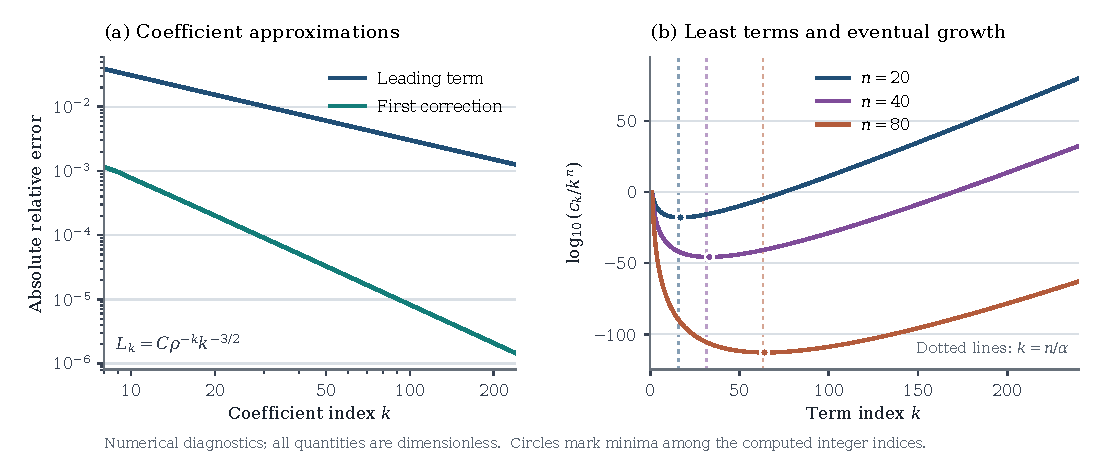
\includegraphics[width=\linewidth]{../reports/gaussian-parity-reductions/figures/14-exact-reductions-moment_asymptotics.pdf}
\caption{Numerical diagnostics for the proved coefficient and moment
asymptotics. Left: absolute relative errors of
\(C\rho^{-k}k^{-3/2}\) and
\(C\rho^{-k}k^{-3/2}(1+\beta_1/k)\), using coefficients computed from
their positive defining recurrence. Right:
\(\log_{10}(c_k/k^n)\) for \(n=20,40,80\). Dotted vertical lines
mark \(k=n/\alpha\); circles mark the sampled minima.
All plotted quantities are dimensionless. The figure illustrates
the theorems and supplies no independent error certificate.}
\label{gaussian:fig:moment-asymptotics}
\end{figure}

\section{Sharp truncation of the log-gamma moment expansion}
Use the constants $\tau,\rho,C$ of the preceding late-coefficient theorem,
and put $\Lambda=-\log\rho$. In this section write $b_k=c_k>0$ for those
positive coefficients, and $\widetilde c_k=(-1)^{k-1}b_k$. The real inverse
$g(t)$ of $1/\Gamma(x)$ on $0\le x\le1$ satisfies $g(t)=-h(-t)$, where
$h(w)=w\Gamma(1-h(w))$ is the earlier inverse germ. Thus
$g(t)=\sum_{k\ge1}\widetilde c_k t^k$ near zero. The moment integral is
\[
 m_n:=M_n/n!=\frac1{\Gamma(n)}\int_0^\infty y^{n-1}g(e^{-y})\,dy.
\]
The first relative coefficient $d_1$ below is the earlier $\beta_1$.
Set $P=\psi'(-\tau)$, $Q=\psi''(-\tau)$, and $R=\psi^{(3)}(-\tau)$; equivalently
$d_1=R/(8P^2)-5Q^2/(24P^3)$.

\begin{lemma}[The dominant inverse singularity]\label{sharp:lem:slit}
The germ $g$ continues to a slit disk of radius greater than $\rho$,
with its only singularity on $|t|=\rho$ at $t=-\rho$, a square-root branch point.
\end{lemma}
\begin{proof}
The positive inverse $h$ has $h(\rho)=\tau$ and is absolutely convergent on
that circle. Its positive coefficients of degrees one and two imply
$|h(t)|<\tau$ at every other point of the circle. With
$\Phi(u)=\Gamma(1-u)$, one then has
$|t\Phi'(h(t))|\le\rho\Phi'(|h(t)|)<\rho\Phi'(\tau)=1$.
The implicit-function theorem continues the inverse across those points.
At $t=\rho$, local inversion at the simple critical point gives a convergent
square-root expansion. Compactness supplies a slightly larger slit disk;
replace $t$ by $-t$ for $g$. This verifies the usual smooth implicit-function
hypotheses directly.\cite{sharp:FS}
\end{proof}
\subsection{A uniform Taylor-remainder lemma}

The next statement is the key passage from fixed-order asymptotics to
optimal truncation. It explicitly crosses the radius of convergence on
the positive real axis; merely summing an infinite Taylor tail there
would be invalid.

\begin{lemma}[Uniform inverse remainder]\label{sharp:lem:inverse-remainder}
For some \(\delta>0\), uniformly for
\(t\in[\rho e^{-\delta},\rho e^\delta]\), put \(r=t/\rho\). Then
\begin{equation}\label{sharp:eq:inverse-remainder}
 \frac{g(t)-\sum_{k=1}^{N-1}\widetilde c_kt^k}{\widetilde c_Nt^N}
 =\frac1{1+r}+\frac{3r}{2N(1+r)^2}+O(N^{-2}).
\end{equation}
On each of the remaining real intervals
\(0<t\leq\rho e^{-\delta}\) and
\(\rho e^\delta\leq t\leq1\), the same normalized remainder is
bounded uniformly in \(N\) sufficiently large.
\end{lemma}

\begin{proof}
The preceding theorem gives a slit disk of continuation for \(g\),
with its only singularity at \(-\rho\).
Choose its outer radius \(R>\rho\), and then \(\delta>0\) so small that
\(\rho e^\delta<R\) and \(\rho e^\delta<1\).
Cauchy's integral formula for \(g(t)\), less its first \(N-1\)
Taylor terms, has kernel \(t^N/(z^N(z-t))\). Deform its contour to the
two banks of the negative cut and an outer contour.
The coefficient \(\widetilde c_N\) uses kernel \(z^{-N-1}\).
On the cut \(z=-s\), the ratio of these kernels, after removing
\(t^N\), is
\[
 \frac{z}{z-t}=\frac{s}{s+t}.
\]
The jump of \(g\) at \(s=\rho\) is a nonzero constant times
\((s-\rho)^{1/2}(1+O(s-\rho))\), with a complete expansion.
The coefficient integral is thus a Watson-type endpoint integral
whose normalized variable \(u=(s-\rho)/\rho\) has
\[
 \langle u\rangle=\frac{3}{2N}+O(N^{-2}),
 \qquad \langle u^2\rangle=O(N^{-2}).
\]
These formulas follow directly by comparing
\(\int_0^\epsilon u^{j+1/2}(1+u)^{-N-1}\dd u\)
with its beta integral extended to infinity. Terms outside a fixed
small neighborhood of zero are exponentially smaller.
Expanding
\[
 \frac{s}{s+t}
 =\frac1{1+r}+\frac{r}{(1+r)^2}u+O(u^2)
\]
proves \eqref{sharp:eq:inverse-remainder}.
The outer contour contributes \(O(R^{-N})\) to the coefficient and
\(O((t/R)^N)\) to the remainder; after normalization these errors are
exponentially small uniformly on the stated compact \(t\)-interval.
This contour argument defines and estimates the actual analytic
remainder on both sides of \(t=\rho\).

It remains to bound the two outer real intervals.
The estimate \(b_k\asymp\rho^{-k}k^{-3/2}\) implies that, below
\(\rho e^{-\delta}\), the absolutely convergent tail is bounded by
a constant times \(b_Nt^N\). Above \(\rho e^\delta\), use
\[
 \sum_{k<N}\frac{b_kt^k}{b_Nt^N}
 \ll\sum_{k<N}(N/k)^{3/2}(\rho/t)^{N-k}.
\]
Splitting at \(k=N/2\) bounds this uniformly by a geometric series
plus an exponentially small term times a polynomial in \(N\).
Furthermore \(0\leq g(t)\leq1\), whereas \(b_Nt^N\) grows
exponentially uniformly on this interval. This proves the last claim.
\end{proof}

\subsection{Sharp optimal truncation}

\begin{theorem}[Half the first omitted term]\label{sharp:thm:optimal-moment}
Let \(n,N\) tend to infinity through positive integers with
\(\eta=N\Lambda-n\) in a fixed bounded interval. Then
\begin{equation}\label{sharp:eq:optimal-moment}
 \boxed{\displaystyle
 m_n-\sum_{k=1}^{N-1}\frac{(-1)^{k-1}b_k}{k^n}
 =\frac{(-1)^{N-1}b_N}{N^n}
 \left(\frac12+\frac{3-2\eta}{8N}+O(N^{-2})\right).}
\end{equation}
The \(O\)-constant is uniform for bounded \(\eta\).
The ratio in parentheses has a complete asymptotic expansion in
\(1/N\), with coefficients computable from the local inverse expansion
and gamma moments.
In particular, taking the nearest integer to \((n+3/2)/\Lambda\)
gives a rigorously justified least-term approximation. The error
eventually has the sign of the first omitted term and is asymptotic
to one half of that term.
\end{theorem}

\begin{proof}
Subtract the finite sum under \eqref{gaussian:eq:moment-inverse}, using
\[
 \frac1{(n-1)!}\int_0^\infty y^{n-1}e^{-ky}\dd y=k^{-n}.
\]
With \(Y\) having the gamma density
\(N^ny^{n-1}e^{-Ny}/(n-1)!\), the error divided by \(\widetilde c_N/N^n\) is
the expectation of the normalized inverse remainder at \(t=e^{-Y}\).

The gamma distribution concentrates at \(\Lambda\):
\[
 \E Y=\frac nN=\Lambda-\frac\eta N,\qquad
 \operatorname{Var}Y=\frac n{N^2}.
\]
For every fixed small \(\delta>0\), its probability outside
\([\Lambda-\delta,\Lambda+\delta]\) is \(O(e^{-a_\delta N})\).
This follows from its moment-generating function
\((1-u/N)^{-n}\) and Chernoff's inequality.
The uniform outer bounds in Lemma~\ref{sharp:lem:inverse-remainder}
therefore make the outer contribution exponentially small.

On the middle interval, the leading kernel is
\[
 L(Y-\Lambda)=\frac1{1+e^{\Lambda-Y}},\qquad
 L(v)=\frac12+\frac v4-\frac{v^3}{48}+O(v^4).
\]
Writing \(V=Y-\Lambda\), its centered gamma moments give
\[
 \E V=-\frac\eta N,\qquad
 \E V^3=O(N^{-2}),\qquad \E V^4=O(N^{-2}),
\]
uniformly for bounded \(\eta\). Thus
\(\E L(V)=1/2-\eta/(4N)+O(N^{-2})\).
It is essential here to use the signed third moment; an absolute
cubic bound alone would lose half a power.
The correction kernel in \eqref{sharp:eq:inverse-remainder} is
\[
 \frac{3e^{-V}}{2N(1+e^{-V})^2}.
\]
Its value at zero is \(3/(8N)\), and its first derivative vanishes
there, so its expectation is \(3/(8N)+O(N^{-2})\).
Adding these terms proves \eqref{sharp:eq:optimal-moment}.
The contour calculation and the Taylor/gamma-moment calculation can
both be continued to arbitrary fixed order. Gamma central moments
are polynomials in \(n\) and \(N^{-1}\); their parity and degree give
integer powers of \(N^{-1}\).
\end{proof}

The theorem strengthens the classical expansion in two ways.
It allows \(N\) to grow linearly with \(n\), and it estimates the
actual error after truncation. The least-term estimate alone would
not justify either conclusion. No global sign assertion for every
\(n,N\) is needed.

\begin{corollary}[Second correction]\label{sharp:cor:moment-second}
Under the hypotheses of Theorem~\ref{sharp:thm:optimal-moment}, the normalized
error has the more precise expansion
\begin{align}
 \frac{m_n-\sum_{k<N}\widetilde c_k/k^n}{\widetilde c_N/N^n}
 &=\frac12+\frac{3-2\eta}{8N}\notag\\
 &\quad+\frac1{N^2}
 \left(\frac{d_1}{4}+\frac{\Lambda(6\eta-13)}{96}\right)
 +O(N^{-3}).\label{sharp:eq:moment-second}
\end{align}
\end{corollary}

\begin{proof}
Here are the additional local coefficients, so that the assertion is
independently reproducible. Let \(v=B-\tau\), and use \(P,Q,R\)
from \eqref{sharp:lem:slit}. The characteristic inverse satisfies
\[
 \log\frac{B/\Gamma(1-B)}{\rho}
 =-\frac{P}{2}v^2+\frac{Q}{6}v^3-\frac{R}{24}v^4+O(v^5).
\]
Putting \(w=\sqrt{1-t/\rho}\) and
\(\alpha_*=\sqrt{2/P}\), inversion gives
\[
 B(t)=\tau-\alpha_* w+\frac{Q}{3P^2}w^2+\mu w^3+O(w^4),
 \qquad
 D:=\frac{\mu}{\alpha_*}
 =-\frac14+\frac{R}{12P^2}-\frac{5Q^2}{36P^3}.
\]
Thus the positive cut density for \(B\) is
\((\alpha_*/\pi)u^{1/2}(1+Du+O(u^2))\), where \(u=t/\rho-1\).
Transfer gives \(d_1=3/8+3D/2\), proving
\eqref{sharp:lem:slit} as well. The normalized endpoint moments are
\[
 \langle u\rangle=\frac{3}{2N}
       +\frac{9/4+3D/2}{N^2}+O(N^{-3}),\qquad
 \langle u^2\rangle=\frac{15}{4N^2}+O(N^{-3}),\qquad
 \langle u^3\rangle=O(N^{-3}).
\]
They follow from beta integrals and the displayed cut density.
The coefficient of \(N^{-2}\) in the inverse remainder at \(r=t/\rho\)
is therefore
\[
 K_2(r)=\frac{r}{(1+r)^2}\left(\frac94+\frac{3D}{2}\right)
                    -\frac{15r}{4(1+r)^3},\qquad K_2(1)=d_1/4.
\]
For the gamma average, put
\(K_1(v)=3e^{-v}/[2(1+e^{-v})^2]\) and \(V=Y-\Lambda\).
Taylor expansion through degree five, using
\(\E|V|^6=O(N^{-3})\), gives
\[
 \E L(V)=\frac12-\frac{\eta}{4N}
       +\frac{\Lambda(3\eta-2)}{48N^2}+O(N^{-3}),\qquad
 \E K_1(V)=\frac38-\frac{3\Lambda}{32N}+O(N^{-2}).
\]
For example \(\E V^3=\Lambda(2-3\eta)N^{-2}+O(N^{-3})\);
the signed fifth moment is \(O(N^{-3})\).
Also \(\E K_2(e^{-V})=K_2(1)+O(N^{-1})\).
The uniform outer bound again makes all outer contributions
exponentially small. Combining the three terms proves
\eqref{sharp:eq:moment-second}.
\end{proof}

\begin{figure}[t]
 \centering
 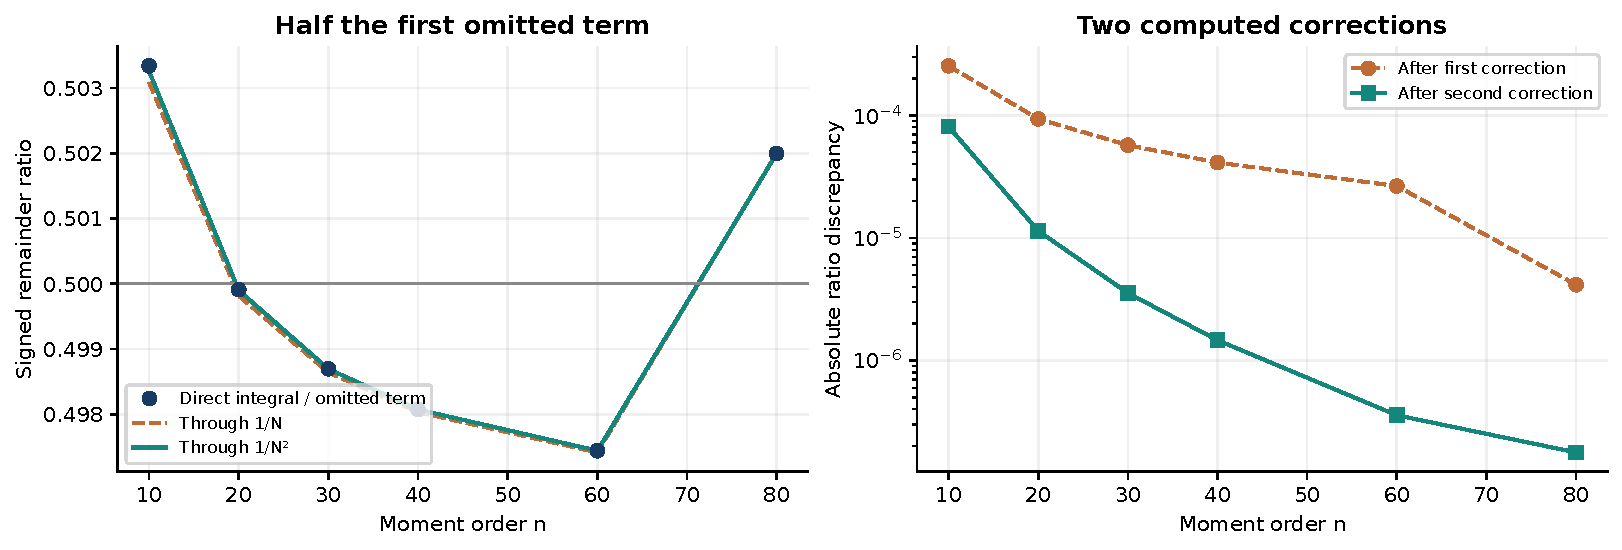
\includegraphics[width=\textwidth]{../reports/reflection-euler-tornheim/figures/moment_remainders.pdf}
 \caption{The signed error divided by the first omitted term, at a
 truncation near \((n+3/2)/\Lambda\). The first-correction formula tracks
 the small changes caused by rounding the truncation index. The plot is
 numerical corroboration; Theorem~\ref{sharp:thm:optimal-moment} supplies the proof.}
 \label{sharp:fig:moments}
\end{figure}

\subsection{A convergent identity with an explicit tail bound}

An asymptotic series should not be used as an infinite exact sum.
The same inverse coordinate gives an exact convergent alternative.

\begin{proposition}[Cutoff identity]\label{sharp:prop:cutoff}
For \(n\geq1\) and \(Y>\Lambda\),
\begin{equation}\label{sharp:eq:cutoff}
 m_n=\frac1{(n-1)!}\int_0^Y y^{n-1}g(e^{-y})\dd y
      +\sum_{k\geq1}\frac{\widetilde c_k}{k^n}Q(n,kY),
 \qquad
 Q(n,z)=e^{-z}\sum_{j=0}^{n-1}\frac{z^j}{j!}.
\end{equation}
The sum is absolutely convergent. If \(Y>\log4\), the absolute tail
after \(k=K\) is at most
\begin{equation}\label{sharp:eq:cutoff-bound}
 \frac{(4e^{-Y})^{K+1}}{2(1-4e^{-Y})}
 \sum_{j=0}^{n-1}\frac{Y^j}{j!(K+1)^{n-j}}.
\end{equation}
\end{proposition}

\begin{proof}
Split \eqref{gaussian:eq:moment-inverse} at \(Y\), substitute the convergent inverse
series on the tail, and integrate term by term.
The coefficient growth theorem proves absolute convergence.
For the elementary explicit bound, note that
\[
 \frac{1/2}{\Phi(1/2)}=\frac1{2\sqrt\pi}>\frac14.
\]
The smaller solution to \(B=t\Phi(B)\) at \(t=1/4\) is therefore
less than \(1/2\); equivalently \(B(1/4)<1/2\).
Positivity gives \(b_k\leq4^k/2\).
For \(k>K\) and \(j\leq n-1\), \(k^{j-n}\leq(K+1)^{j-n}\).
The geometric tail now gives \eqref{sharp:eq:cutoff-bound}.
\end{proof}

The numerical implementation uses ordinary high-precision arithmetic
and explicitly distinguishes analytic truncation bounds from interval
rounding bounds. Formula \eqref{sharp:eq:cutoff} is also suitable for a future
ball-arithmetic evaluator: the finite inverse integral and all constant
evaluations can be enclosed separately.


% Parent document supplies amsmath, amssymb, amsthm, and theorem environments.
% Bibliography key ACEMKM is specified in gamma_provenance.txt.
\section{Reflected log-gamma moments and their late coefficients}
\label{reflected:sec:reflected-moments}

Set $f(x)=\log\Gamma(x)$ for $0<x<1$, and define
\[
 M_{n,m}=\int_0^1 f(x)^n f(1-x)^m\,dx,
 \qquad n,m\in\mathbb Z_{\ge0}.
\]
These integrals already occur as $T_{n+m,n}$ in
Amdeberhan et al.\ \cite[Section~5]{gaussian:ACEMKM}.  Their symmetry
$M_{n,m}=M_{m,n}$ and the identities obtained by expanding Euler's
reflection formula are therefore classical.  The asymptotic question here
is different: keep the reflected exponent $m$ fixed and let $n$ tend to
infinity.  The factor $f(1-x)^m$ vanishes to order $m$ at the endpoint
that produces the factorial growth.  This shifts the first exponential
scale from $1$ to $m+1$ without removing the eventual divergence of the
full expansion.  Theorem~\ref{reflected:gam:thm:late} identifies its late terms,
including their signs and the first relative correction.

\subsection{The meromorphic transform and all finite asymptotic orders}

Put
\[
 B(x)=\log\Gamma(1-x)
 =\gamma x+\sum_{j\ge2}\frac{\zeta(j)}j x^j,
 \qquad |x|<1,
\]
where $\gamma$ is Euler's constant.  For $k\ge1$ define
\begin{equation}\label{reflected:gam:eq:residue-coefficients}
 A_{k,m}=\frac1k[x^{k-1}]\exp\{kB(-x)\}B(x)^m.
\end{equation}
The convention $B(x)^0=1$ is in force.  In particular $A_{k,m}=0$
when $k\le m$.  Every coefficient is a finite polynomial over
$\mathbb Q$ in $\gamma,\zeta(2),\ldots,\zeta(k-1)$.

\begin{theorem}[Reflected moment expansion]\label{reflected:gam:thm:expansion}
For each fixed integer $m\ge0$, the function
\[
 F_m(z)=\int_0^1\Gamma(x)^z f(1-x)^m\,dx
\]
is holomorphic for $\operatorname{Re}z<m+1$, has Taylor expansion
\[
 F_m(z)=\sum_{n\ge0}\frac{M_{n,m}}{n!}z^n
 \qquad (|z|<m+1),
\]
and extends meromorphically to $\mathbb C$.  Its only possible poles
are simple poles at integers $k\ge m+1$, with
\begin{equation}\label{reflected:gam:eq:poles}
 \operatorname*{Res}_{z=k}F_m(z)=-kA_{k,m}.
\end{equation}
The first pole is present.  For every fixed integer $K\ge m+1$,
\begin{equation}\label{reflected:gam:eq:fixed-expansion}
 \frac{M_{n,m}}{n!}
 =\sum_{k=m+1}^{K}\frac{A_{k,m}}{k^n}
   +O_{m,K}\bigl((K+1)^{-n}\bigr),\qquad n\longrightarrow\infty.
\end{equation}
Consequently
\begin{equation}\label{reflected:gam:eq:leading}
 M_{n,m}\sim \frac{\gamma^m n!}{(m+1)^{n+1}}.
\end{equation}
\end{theorem}

\begin{proof}
As $x\downarrow0$, $f(x)=-\log x+O(x)$ and
$B(x)=\gamma x+O(x^2)$.  At the other endpoint,
$f(x)=O(1-x)$ and $f(1-x)=O(1+|\log(1-x)|)$.
These estimates prove absolute convergence and compact domination in
the asserted half-plane, including after any number of differentiations
in $z$.  They also justify the Taylor expansion near zero.

Fix $0<a<1$ and an integer $J\ge1$.  Taylor expansion in $x$ gives
\[
 \Gamma(1+x)^z B(x)^m
 =\sum_{j=0}^{J-1}b_{j,m}(z)x^j+x^J E_{J,m}(x,z),
\]
where each $b_{j,m}$ is an entire function of $z$, and the remainder is
uniformly bounded for $0\le x\le a$ and $z$ in compact sets.
The integral over $[0,a]$ is therefore
\[
 \sum_{j=0}^{J-1}\frac{b_{j,m}(z)a^{j+1-z}}{j+1-z}
 +\int_0^a x^{J-z}E_{J,m}(x,z)\,dx.
\]
The last integral is holomorphic for $\operatorname{Re}z<J+1$.
The integral over $[a,1]$ is entire, since its logarithmic singularity
at $1$ is integrable uniformly for $z$ in compact sets.  Letting $J$
increase gives the continuation.  At $z=k$ its residue is
$-b_{k-1,m}(k)=-kA_{k,m}$.  Since $B(x)^m$ starts with
$\gamma^m x^m$, the first nonzero coefficient is
$A_{m+1,m}=\gamma^m/(m+1)>0$.

For the asymptotic assertion, subtract the polar functions
\[
 \sum_{k=m+1}^{K+1}\frac{kA_{k,m}}{k-z}
\]
from $F_m(z)$.  The difference is holomorphic on $|z|<K+2$.
Cauchy's estimate on any circle $K+1<R<K+2$ bounds its $n$th Taylor
coefficient by $O_{m,K,R}(R^{-n})$.  Restoring the term at $K+1$
proves \eqref{reflected:gam:eq:fixed-expansion}, even if that particular coefficient
happens to vanish.  Taking $K=m+1$ proves \eqref{reflected:gam:eq:leading}.
\end{proof}

The first three coefficients are explicit.  Write $k=m+3$ in the last line:
\begin{align}
 A_{m+1,m}&=\frac{\gamma^m}{m+1},\label{reflected:gam:eq:first-three}\\
 A_{m+2,m}&=\frac{\gamma^{m-1}}{m+2}
 \left(\frac{m\zeta(2)}2-(m+2)\gamma^2\right),\notag\\
 A_{m+3,m}&=\frac{\gamma^m}{k}
 \left\{\frac{m\zeta(3)}{3\gamma}
 +\frac{m(m-1)\zeta(2)^2}{8\gamma^2}
 +\frac{k(1-m)\zeta(2)}2+\frac{k^2\gamma^2}2\right\}.\notag
\end{align}
These displays also apply to $m=0$, since $\gamma>0$ and factors of
$m$ remove the superfluous terms.  For example,
\begin{align*}
 \frac{M_{n,1}}{n!}
 &=\frac{\gamma}{2^{n+1}}
 +\frac{\zeta(2)/2-3\gamma^2}{3^{n+1}}
 +\frac{\zeta(3)/3+8\gamma^3}{4^{n+1}}+O(5^{-n}),\\
 \frac{M_{n,2}}{n!}
 &=\frac{\gamma^2}{3^{n+1}}
 +\frac{\gamma\zeta(2)-4\gamma^3}{4^{n+1}}+O(5^{-n}).
\end{align*}
The second displayed correction is positive, whereas the corresponding
correction for $m=1$ is negative.  Thus strict alternation from the first
term cannot be imported from the unreflected family.  The two signs can,
for instance, be checked using the elementary enclosures
$0.577<\gamma<0.578$ and $1.644<\zeta(2)<1.646$.
Eventual alternation has a different, precise rule.

\subsection{Late coefficients and a universal inverse-gamma scale}

Let $\phi(u)=\Gamma(1-u)$ and $D=u\,d/du$.  Define $\tau\in(0,1)$ by
\begin{equation}\label{reflected:gam:eq:critical}
 D\log\phi(\tau)=-\tau\psi(1-\tau)=1,
\end{equation}
and put
\begin{equation}\label{reflected:gam:eq:constants}
 \rho=\frac{\tau}{\phi(\tau)},\quad
 v=D^2\log\phi(\tau)=1+\tau^2\psi'(1-\tau),\quad
 C=\frac{\tau}{\sqrt{2\pi v}},\quad
 b=-\log\Gamma(1+\tau).
\end{equation}
The equation for $\tau$ has a unique solution: its left side equals
$\gamma u+\sum_{j\ge2}\zeta(j)u^j$, which is strictly increasing from
zero to infinity.  Also $0<\rho<1$ and $b>0$, the latter by strict
log-convexity of $\Gamma$ between $1$ and $2$.  Numerically,
$\tau=0.5040830082\ldots$ and $\rho=0.2821158090\ldots$.
Only the exact definitions are used below.

\begin{theorem}[Late reflected coefficients]\label{reflected:gam:thm:late}
For every fixed nonnegative integer $m$,
\begin{equation}\label{reflected:gam:eq:late}
 A_{k,m}=(-1)^{k+m-1}C b^m\rho^{-k}k^{-3/2}
 \left(1+\frac{\beta_m}{k}+O_m(k^{-2})\right).
\end{equation}
There is a full asymptotic expansion in integer powers of $1/k$.
To specify the first correction, set
$G(u)=\log\Gamma(1+u)$, $H_m(u)=G(u)^m$, and
$\kappa_j=D^j\log\phi(\tau)$.  All quantities on the right below
are evaluated at $u=\tau$:
\begin{equation}\label{reflected:gam:eq:beta}
 \beta_m=
 -\frac{(D+1)^2H_m}{2vH_m}
 +\frac{\kappa_3(D+1)H_m}{2v^2H_m}
 +\frac{\kappa_4}{8v^2}
 -\frac{5\kappa_3^2}{24v^3}.
\end{equation}
In particular, every sufficiently large possible pole in
Theorem~\ref{reflected:gam:thm:expansion} is present.  More explicitly,
\[
 \operatorname{Res}_{z=k}F_m(z)
 =(-1)^{k+m}C b^m\rho^{-k}k^{-1/2}
   \left(1+\frac{\beta_m}{k}+O_m(k^{-2})\right),
\]
so the eventual residue sign is $(-1)^{k+m}$.  For every fixed real $n$, the formal series
$\sum_{k\ge m+1}A_{k,m}/k^n$ diverges because its terms do not tend to zero.
\end{theorem}

\begin{proof}
Replacing $x$ by $-u$ in \eqref{reflected:gam:eq:residue-coefficients} gives
\[
 A_{k,m}=\frac{(-1)^{k-1}}k[u^{k-1}]\phi(u)^k H_m(u).
\]
The function $H_m$ is holomorphic for $|u|<1$.  If
$\phi(u)=\sum_{j\ge0}a_ju^j$, all the $a_j$ are strictly positive,
since $\log\phi$ has positive coefficients.  Thus
\[
 p_j=\frac{a_j\tau^j}{\phi(\tau)}
\]
is a probability distribution with exponential moments, mean one,
variance $v>0$, and positive mass at both $0$ and $1$.  It follows
that the function
\[
 Q(t)=\frac{\phi(\tau e^{it})}{\phi(\tau)}e^{-it}
\]
has modulus strictly less than one for $0<|t|\le\pi$, while
\[
 \log Q(t)=-\frac v2t^2-\frac{i\kappa_3}6t^3
 +\frac{\kappa_4}{24}t^4+O(t^5)
\]
near zero.  Cauchy's coefficient formula becomes
\begin{equation}\label{reflected:gam:eq:cauchy}
 A_{k,m}=
 \frac{(-1)^{k-1}\tau\rho^{-k}}{2\pi k}
 \int_{-\pi}^{\pi}Q(t)^k e^{it}H_m(\tau e^{it})\,dt.
\end{equation}

Fix a sufficiently small $\delta>0$.  On $\delta\le|t|\le\pi$
the integral is $O(q^k)$ for some $q<1$.  On
$k^{-2/5}\le|t|\le\delta$ it is $O(e^{-c k^{1/5}})$, because
$|Q(t)|\le e^{-ct^2}$.  The analytic amplitude is bounded on the
whole circle.  On the remaining interval set $t=y/\sqrt{k}$.
Gaussian domination and Taylor expansion to any fixed order, with
an analytic remainder, give a full expansion.  Odd terms integrate
to zero, so only integer powers of $1/k$ occur.  The leading integral is
\[
 H_m(\tau)\sqrt{\frac{2\pi}{vk}}
 =(-1)^m b^m\sqrt{\frac{2\pi}{vk}},
\]
which proves the leading term in \eqref{reflected:gam:eq:late}.

For the first correction, the amplitude derivatives at $t=0$ are
$H_m$, $i(D+1)H_m$, and $-(D+1)^2H_m$.
The Gaussian moments of degrees $2$, $4$, and $6$ contribute,
respectively, the amplitude's quadratic term, the amplitude--cubic
cross term together with the quartic phase term, and the square of
the cubic phase term.  Their normalized sum is exactly
\eqref{reflected:gam:eq:beta}.  Expanding two further even orders gives a
relative $O_m(k^{-2})$ remainder after the displayed correction.
Since $C b^m>0$ and $\rho<1$, the assertions about nonvanishing,
signs, and divergence follow at once.
\end{proof}

This proof uses the circle $|u|=\tau$ and a strict modulus inequality;
it does not presume a classification of all complex critical values
of the reciprocal gamma function.  The same circle governs every fixed
reflected exponent.  With $\alpha=-\log\rho$, the continuous minimum
of the leading term magnitude $\rho^{-k}k^{-n-3/2}$ occurs at
$k=(n+3/2)/\alpha$.  A least-term calculation alone does not bound the
remainder.  The next result supplies an explicit bound with a growing
number of terms.

\subsection{An effective remainder despite the initial sign changes}

\begin{theorem}[Explicit reflected truncation bound]\label{reflected:gam:thm:effective}
Let $m\ge0$, $n\ge1$, and $K\ge1$ be integers, put
$\alpha=-\log\rho$ and $T_m=\tau B(\tau)^m$, and suppose $K\alpha<n$.
With
\[
 R^{(m)}_{n,K}=\frac{M_{n,m}}{n!}
             -\sum_{k=1}^K\frac{A_{k,m}}{k^n},
 \qquad \Gamma(n,s)=\int_s^\infty t^{n-1}e^{-t}\,dt,
\]
one has the entirely explicit estimate
\begin{align}\label{reflected:gam:eq:effective}
 |R^{(m)}_{n,K}|\le{}&\frac{\alpha^n}{n!}
 \left(m!+\frac{nT_m}{n-K\alpha}\right)\notag\\
 &+\frac{T_m\rho^{-K-1}}{(K+1)^n}
          \frac{\Gamma(n,(K+1)\alpha)}{\Gamma(n)}.
\end{align}
If $n\ge\max\{2,4\alpha^2\}$ and
$K=\lfloor n/\alpha-\sqrt n\rfloor$, then $K\ge1$ and
\begin{equation}\label{reflected:gam:eq:optimized}
 |R^{(m)}_{n,K}|\le
 \left(\frac{m!}{\sqrt{2\pi n}}+
       \frac{T_m}{\alpha\sqrt{2\pi}}+T_m e^{2\alpha^2}\right)
 \left(\frac{e\alpha}{n}\right)^n.
\end{equation}
This bound holds for every $m$, but no useful uniform relative error is
asserted when $m$ grows with $n$.
\end{theorem}
\begin{proof}
The function $f$ decreases from infinity to zero on $(0,1]$:
$\psi'(x)>0$ and $\psi(1)=-\gamma<0$.  Let $x(y)$ denote its inverse,
and set $W_m(x)=\int_0^x B(t)^m\,dt$.  Tonelli's theorem applied to
$f(x)^n=n\int_0^{f(x)}y^{n-1}\,dy$ gives
\begin{equation}\label{reflected:gam:eq:layercake}
 \frac{M_{n,m}}{n!}
 =\frac1{\Gamma(n)}\int_0^\infty y^{n-1}W_m(x(y))\,dy.
\end{equation}

Let $h(q)$ be the local solution of $h=q\phi(h)$ with $h(0)=0$.
Lagrange inversion gives positive coefficients
\[
 h(q)=\sum_{k\ge1}c_kq^k,
 \qquad c_k=\frac1k[u^{k-1}]\phi(u)^k.
\]
The $m=0$ case of Theorem~\ref{reflected:gam:thm:late} proves that its radius
is $\rho$ and that the series converges absolutely on $|q|\le\rho$.
The map $u\mapsto u/\phi(u)$ increases strictly from $0$ to $\rho$
on $[0,\tau]$, so inversion along this interval and continuity imply
$h(\rho)=\tau$.  No other inverse branch is used.

Lagrange--B\"urmann inversion now gives
\[
 W_m(x(y))=\sum_{k\ge1}A_{k,m}e^{-ky}
 \qquad(y\ge\alpha).
\]
Indeed $x(y)=-h(-e^{-y})$ initially for large $y$, and then throughout
$y>\alpha$ by analytic continuation along the strictly monotone real
inverse.  The endpoint follows by absolute convergence.  To prove that
convergence and obtain its quantitative majorant, define
\[
 d_{k,m}=\frac1k[u^{k-1}]\phi(u)^k B(u)^m\ge0.
\]
Coefficientwise absolute values in $B(-u)^m$ are $B(u)^m$.
Consequently $|A_{k,m}|\le d_{k,m}$, while another application of
Lagrange--B\"urmann gives
\[
 \sum_{k\ge1}d_{k,m}\rho^k=W_m(h(\rho))=W_m(\tau)
 \le\tau B(\tau)^m=T_m.
\]
Here $B$ has positive Taylor coefficients and is increasing on $[0,\tau]$.
Thus on $y\ge\alpha$,
\[
 \left|W_m(x(y))-\sum_{k=1}^K A_{k,m}e^{-ky}\right|
 \le T_m\rho^{-K-1}e^{-(K+1)y}.
\]
Its integral in \eqref{reflected:gam:eq:layercake} is the second term of
\eqref{reflected:gam:eq:effective}.

On $0\le y\le\alpha$, use $0\le W_m(x(y))\le M_{m,0}\le m!$.
The last inequality follows from
$0\le\log\Gamma(x)\le-\log x$, since log-convexity gives
$\Gamma(1+x)\le1$ for $0\le x\le1$.  Also, for $k\le K$,
\[
 \int_0^\alpha y^{n-1}e^{-ky}\,dy
 \le\frac{\alpha^n e^{-k\alpha}}{n-k\alpha}.
\]
This follows by differentiating $y^ne^{-ky}$ and using
$n-ky\ge n-k\alpha>0$.  Summing with
$\sum|A_{k,m}|\rho^k\le T_m$ proves the first term of
\eqref{reflected:gam:eq:effective}.

For the stated choice of $K$, $n-K\alpha\ge\alpha\sqrt n$ and
$\theta=(K+1)\alpha/n$ lies in $[1/2,1]$.
The inequality $\theta-1-\log\theta\le2(1-\theta)^2$ gives
\[
 \rho^{-K-1}(K+1)^{-n}
 \le e^{2\alpha^2}(e\alpha/n)^n.
\]
Finally, $\Gamma(n,s)\le\Gamma(n)$ and
$n!\ge\sqrt{2\pi n}(n/e)^n$ yield \eqref{reflected:gam:eq:optimized}.
\end{proof}

\subsection{Sharp truncation for every fixed reflected exponent}
The reflected coefficient expansion and the sharp inverse remainder now
combine. This statement uses the two incoming developments together;
it is stronger than their separate absolute-bound and unreflected results.
Write $\Lambda=-\log\rho$, and retain $\beta_m$ from
\eqref{reflected:gam:eq:beta}.

\begin{corollary}[Half the first omitted reflected term]
\label{reflected:cor:sharp}
Fix an integer $m\ge0$. Let $n,N\to\infty$ through positive integers,
with $\eta=N\Lambda-n$ in a fixed bounded interval. Then
\begin{align}\label{reflected:eq:sharp}
 \frac{M_{n,m}/n!-\sum_{k=1}^{N-1}A_{k,m}/k^n}{A_{N,m}/N^n}
 ={}&\frac12+\frac{3-2\eta}{8N}\notag\\
 &+\frac1{N^2}\left[\frac{\beta_m}{4}
       +\frac{\Lambda(6\eta-13)}{96}\right]+O_m(N^{-3}),
\end{align}
uniformly for bounded $\eta$. In particular the error eventually has
sign $(-1)^{N+m-1}$ and is asymptotic to half the first omitted term.
The denominator is nonzero for every sufficiently large $N$.
\end{corollary}
\begin{proof}
Set $W_m(x)=\int_0^x B(u)^m\,du$ and $G_m(t)=W_m(g(t))$, where $g$ is
the real inverse used in the preceding sharp-moment section.
Lagrange--B\"urmann inversion gives
$G_m(t)=\sum_{k\ge1}A_{k,m}t^k$ near zero. The layer-cake formula
\eqref{reflected:gam:eq:layercake} becomes
\[
 M_{n,m}/n!=\frac1{\Gamma(n)}\int_0^\infty y^{n-1}G_m(e^{-y})\,dy.
\]
Since $W_m$ is holomorphic on $|x|<1$, it can be composed with the
slit-disk inverse of Lemma~\ref{sharp:lem:slit}. At the dominant point
$g(-\rho)=-\tau$ its derivative is
\[
 W_m'(-\tau)=B(-\tau)^m
       =\bigl(\log\Gamma(1+\tau)\bigr)^m=(-b)^m\ne0.
\]
Thus $G_m$ has the same sole dominant square-root singularity, with a
nonzero leading amplitude. Its late coefficients have the relative
coefficient $\beta_m$ established in Theorem~\ref{reflected:gam:thm:late}.
The Cauchy cut-contour argument in Lemma~\ref{sharp:lem:inverse-remainder}
therefore applies to $G_m$ with the same leading kernel
$1/(1+t/\rho)$ and the same $3/(2N)$ endpoint-moment correction.
The sign of the leading jump cancels against $A_{N,m}$ in this ratio.
The second normalized cut coefficient at $t=\rho$ is $\beta_m/4$,
by the same square-root transfer and beta-moment calculation used in
Corollary~\ref{sharp:cor:moment-second}.

The outer real-interval bounds also persist. Above the convergence
radius, the finite coefficient sum is bounded using
$|A_{k,m}|\asymp_m\rho^{-k}k^{-3/2}$, while $0\le G_m(t)\le m!$ for
$0\le t\le1$. The finitely many exceptional early coefficients contribute
only an exponentially small term after normalization. Below the radius,
the absolute Taylor tail gives the corresponding uniform bound.
Average the normalized remainder against the gamma density with shape
$n$ and rate $N$. Its signed moments are exactly those used in the
unreflected calculation. The first two corrections are consequently
\eqref{reflected:eq:sharp}, with $d_1$ replaced by $\beta_m$; the analytic
cut expansion and moments through degree six give the stated uniform
$O_m(N^{-3})$ remainder. Eventual nonvanishing and the sign follow from
\eqref{reflected:gam:eq:late}.
\end{proof}
This fixed-$m$ corollary does not supply uniform relative estimates when
$m$ grows with $n$. That joint regime remains a separate problem.

\subsection{An exact identity coupling all reflected residues}

The coefficients across different $m$ satisfy a finite identity in which
Euler's constant and all odd zeta values cancel.

\begin{proposition}[Reflection sum for the residues]\label{reflected:gam:prop:residue-sum}
For every integer $k\ge1$,
\begin{equation}\label{reflected:gam:eq:residue-sum}
 \sum_{m=0}^{k-1}\frac{k^m}{m!}A_{k,m}
 =\begin{cases}
 0,&k\text{ even},\\[2pt]
 \displaystyle\frac{\pi^{k-1}}{k\,2^{k-1}}
 \binom{k-1}{(k-1)/2},&k\text{ odd}.
 \end{cases}
\end{equation}
\end{proposition}
\begin{proof}
Because $B(x)^m$ has order $m$, extending the sum over $m$ to infinity
does not affect $[x^{k-1}]$.  Euler's reflection formula gives
\[
 \sum_{m=0}^{k-1}\frac{k^m}{m!}A_{k,m}
 =\frac1k[x^{k-1}]\bigl(\Gamma(1+x)\Gamma(1-x)\bigr)^k
 =\frac1k[x^{k-1}]\left(\frac{\pi x}{\sin\pi x}\right)^k.
\]
The coefficient is zero for even $k$.  For odd $k$, compute it as
the residue at $x=0$ of $(\pi/\sin\pi x)^k\,dx$.
The local change of variable $t=\sin\pi x$ gives
\[
 [x^{k-1}]\left(\frac{\pi x}{\sin\pi x}\right)^k
 =\pi^{k-1}[t^{k-1}](1-t^2)^{-1/2},
\]
and the binomial expansion proves \eqref{reflected:gam:eq:residue-sum}.
\end{proof}

For example, the cases $k=2,3$ read
$A_{2,0}+2A_{2,1}=0$ and
$A_{3,0}+3A_{3,1}+\tfrac92 A_{3,2}=\pi^2/6$.
They are exact identities among the asymptotic coefficients, rather
than convergent sums of the moment expansions.  No summation over
the late index $k$ is used.

\subsection{A recorded log-sine conjecture has a formal proof}

There is also a small but useful correction to the logical status of
a claim in the literature.  The author preprint of \cite{gaussian:ACEMKM}
labels a coefficient identity as Conjecture~5.5 and motivates it using
transcendence assumptions on $\log 2$ and $\log\pi$.
For the canonical formal polynomials supplied by the beta integral,
the coefficient identity needs none of those assumptions.  Under the
preprint's assumptions these formal coefficients coincide with its
uniquely specified numerical coefficients, so the result also proves
that stated implication.  We do not assert uniqueness of arbitrary
numerical expressions in zeta values and logarithms, nor priority over
any later treatment.

Define polynomials $\mathcal P_N(X)$ by
\begin{equation}\label{reflected:gam:eq:appell-egf}
 \sum_{N\ge0}\mathcal P_N(X)\frac{z^N}{N!}
 =\exp\left\{Xz+\sum_{j\ge2}
       \frac{(1-2^{1-j})\zeta(j)}jz^j\right\}.
\end{equation}
\begin{proposition}[Unconditional coefficient and translation identities]
\label{reflected:gam:prop:appell}
For $N\ge0$,
\begin{align}
 \int_0^1[-\log\sin(\pi x)]^N\,dx&=\mathcal P_N(\log2),\label{reflected:gam:eq:logsine}\\
 [X^j]\mathcal P_N(X)&=\binom Nj \mathcal P_{N-j}(0),\qquad 0\le j\le N,\notag\\
 \sum_{j=0}^N\binom Nj M_{j,N-j}&=\mathcal P_N(\log(2\pi)).\notag
\end{align}
Moreover, the coefficients admit the finite partition formula
\begin{equation}\label{reflected:gam:eq:appell-partitions}
 \mathcal P_N(X)=N!\!\sum_{r_1+2r_2+\cdots+Nr_N=N}
 \frac{X^{r_1}}{r_1!}
 \prod_{j=2}^N\frac1{r_j!}
 \left(\frac{(1-2^{1-j})\zeta(j)}j\right)^{r_j}.
\end{equation}
\end{proposition}
\begin{proof}
For $\operatorname{Re}z<1$, the beta integral gives
\[
 \int_0^1\sin(\pi x)^{-z}\,dx
 =\frac{\Gamma((1-z)/2)}{\sqrt\pi\,\Gamma(1-z/2)}.
\]
Expanding its logarithm at zero gives the right side of
\eqref{reflected:gam:eq:appell-egf} with $X=\log2$; its degree-$j$ coefficient
for $j\ge2$ is $(1-2^{1-j})\zeta(j)/j$.
Extracting Taylor coefficients proves \eqref{reflected:gam:eq:logsine}.
The factor $e^{Xz}$ gives $[X^j]\mathcal P_N=\binom Nj\mathcal P_{N-j}(0)$ by
formal coefficient extraction.  Euler's reflection formula turns
the sum of mixed moments into the integral of
$(\log\pi-\log\sin\pi x)^N$, which translates $X$ by $\log\pi$.
Expanding each exponential factor separately proves
\eqref{reflected:gam:eq:appell-partitions}.  All formal operations in a fixed
degree involve only finitely many coefficients.
\end{proof}

The constant-column generating function has the additional factorization
\begin{equation}\label{reflected:gam:eq:even-odd-factor}
 \sum_{N\ge0}\mathcal P_N(0)\frac{z^N}{N!}
 =\sqrt{\frac{\tan(\pi z/2)}{\pi z/2}}
 \exp\left\{\sum_{\substack{j\ge3\\j\text{ odd}}}
       \frac{(1-2^{1-j})\zeta(j)}jz^j\right\},
\end{equation}
where the square root is the formal branch with constant term one.
Indeed, multiplying the left side by its value at $-z$ and applying
the reflection formula yields $\tan(\pi z/2)/(\pi z/2)$.
The even logarithmic part is therefore the displayed square root.
This makes the multiplicative factorization of its formal odd-zeta
monomial coefficients explicit, while the even-zeta contribution has
an elementary trigonometric generating function.

\paragraph{Verification and remaining questions.}
The accompanying script \src{code/verify_reflected_moments.py} checks the
three coefficient formulas by exact symbolic arithmetic, checks finite
reflection sums and the formal Appell formulas, and compares independent
quadrature with the fixed-order expansion.  It also compares the late
coefficients with \eqref{reflected:gam:eq:late} and \eqref{reflected:gam:eq:beta}.
The numerical calculations are diagnostics; the preceding analytic and
formal arguments are the proofs.
The fixed-reflected-exponent signed remainder is now supplied by
Corollary~\ref{reflected:cor:sharp}. Uniformity when $m$ increases with
$n$ remains a substantive next question.
In the former regime the endpoint approximation
$B(x)^m\approx\gamma^m x^m$ need not be uniform, so the fixed-$m$
theorem does not settle the simultaneous large-exponent problem.


\section{The Stieltjes layer}\label{integral:sec:stieltjes}

Differentiating $L(s,\chi)=q^{-s}\sum_k\chi(k)\,\zeta(s,k/q)$ at $s=1$ gives the exact
ladder
\[
L'(\chi,1)=-\ln q\;L(1,\chi)-\frac1q\sum_k\chi(k)\,\gamma_1\!\Bigl(\frac{k}{q}\Bigr),
\]
so every Malmsten log-log integral is a statement about \emph{first generalized Stieltjes
constants} $\gamma_1(k/q)$ --- Blagouchine's program, equivalent to Deninger's
$\zeta''(0,a)$ layer via the functional equation.

\begin{result}[even-character Malmsten integral]\label{integral:res:evenchi}
\dps{verified to $10^{-51}$; even character mod 5; $\varphi$ the golden ratio}
\[
\int_0^1\ln\ln\frac1x\cdot\frac{(1-x)(1-x^2)}{1-x^5}\,dx
=-(\gamma+\ln5)\,\frac{2\ln\varphi}{\sqrt5}
-\frac{\gamma_1(\tfrac15)-\gamma_1(\tfrac25)-\gamma_1(\tfrac35)+\gamma_1(\tfrac45)}{5}.
\]
\end{result}

\begin{result}[the parity dichotomy]\label{integral:res:parity}
The dichotomy is empirically sharp. The \emph{odd} $\gamma_1$-combination reduces exactly
as differentiated-Kummer predicts \dps{verified blind}:
\[
\gamma_1\!\bigl(\tfrac13\bigr)-\gamma_1\!\bigl(\tfrac23\bigr)
=-\frac{\pi}{\sqrt3}\Bigl(\gamma+4\ln2-\tfrac12\ln3+4\ln\pi-6\ln\Gamma\bigl(\tfrac13\bigr)\Bigr),
\]
which is \emph{Malmsten's 1846 reflection identity} \cite{bridge:Malmsten} (long misattributed
to Almkvist--Meurman). The even combination did not reduce in the tested standard basket
\dps{PSLQ junk at coefficient height $10^8$ --- honest negative}; pushing Blagouchine's
rational-arguments theorem \cite{bridge:BlagouchineJNT} through it collapses everything except a $\zeta''$-block
\dps{derived and verified to $10^{-50}$}:
\[
\gamma_1\!\bigl(\tfrac15\bigr)-\gamma_1\!\bigl(\tfrac25\bigr)
-\gamma_1\!\bigl(\tfrac35\bigr)+\gamma_1\!\bigl(\tfrac45\bigr)
=\sqrt5\,\Bigl[\zeta''\bigl(0,\tfrac15\bigr)-\zeta''\bigl(0,\tfrac25\bigr)
-\zeta''\bigl(0,\tfrac35\bigr)+\zeta''\bigl(0,\tfrac45\bigr)\Bigr]
-2\sqrt5\,\ln\varphi\,\bigl(\gamma+\ln10\pi\bigr).
\]
\end{result}

The canonical atom for the even layer is thus the even-character $\zeta''(0,l/q)$
combination (Deninger's layer \cite{bridge:Deninger}); Malmsten integrals, even $\gamma_1$-combinations, and even
$L'(\chi,1)$ are all elementary-equivalent to it. Two practical records: Blagouchine's
particular value $\gamma_1(1/4)$ was re-verified exactly against \texttt{mpmath}'s
generalized Stieltjes constants, and the reduction coefficients live in
$\mathbb{Q}(\sqrt q)$ --- rational-coefficient PSLQ baskets \emph{miss} the relation, so a
$\sqrt q$-weighted basket or direct derivation is required.
\section{The common Hurwitz-jet calculus}\label{stieltjes:sec:intro}

The generalized Stieltjes constants $\gamma_n(x)$ are defined by the Laurent
expansion of the Hurwitz zeta function at its pole,
\begin{equation}\label{stieltjes:eq:laurent}
\zeta(s,x)=\frac{1}{s-1}+\sum_{n\ge0}\frac{(-1)^n}{n!}\,\gamma_n(x)\,(s-1)^n ,
\end{equation}
so that $\gamma_0(x)=-\psi(x)$ and $\gamma_n(1)=\gamma_n$ are the classical
Stieltjes constants, $\gamma_0=\gamma$. Although universally called
\emph{constants}, the $\gamma_n(x)$ are real-analytic functions of the
argument on $(0,\infty)$, and it is this function-theoretic point of view we
adopt. Following Blagouchine \cite{stieltjes:BlagouchineRJ,bridge:BlagouchineJNT} we write
\[
\Gamma_{\!n}(p)\;:=\;\int_1^p\gamma_n(x)\,dx ,
\qquad\text{so that }\ \Gamma_{\!n}(1)=0 ,
\]
for the antiderivative normalized at $1$. (The notation is Blagouchine's; the
clash with the Euler $\Gamma$-function is resolved by the subscript, and
indeed $\Gamma_{\!0}(p)=-\ln\Gamma(p)$, as Theorem~\ref{stieltjes:thm:ladder} makes
plain.) Throughout, $\zeta^{(k)}(s_0,a):=\partial_s^k\zeta(s,a)\big|_{s=s_0}$
and $\zeta^{(k)}(s_0):=\zeta^{(k)}(s_0,1)$ denote derivative jets with respect
to the \emph{order}; $\Lambda_q:=\gamma+\ln(2\pi q)$; $H_n=\sum_{i\le n}1/i$ and
$H_n^{(2)}=\sum_{i\le n}1/i^2$ are harmonic numbers; $\Glaisher$ is the
Glaisher--Kinkelin constant, $\ln\Glaisher=\tfrac1{12}-\zeta'(-1)$; and
\[
S_j\Bigl(\frac pq\Bigr):=\sum_{k=1}^{q-1}\sin\frac{2\pi kp}{q}\,
\zeta^{(j)}\Bigl(0,\frac kq\Bigr),
\qquad
S_0\Bigl(\frac pq\Bigr)=\tfrac12\cot\frac{\pi p}{q},
\quad
S_1\Bigl(\frac pq\Bigr)=\sum_{k=1}^{q-1}\sin\frac{2\pi kp}{q}\,\ln\Gamma\Bigl(\frac kq\Bigr)
\]
(the closed forms for $S_0,S_1$ use $\zeta(0,a)=\tfrac12-a$,
$\zeta'(0,a)=\ln\Gamma(a)-\tfrac12\lntwopi$, and
$\sum_k\sin(2\pi kp/q)=0$).

The starting observation is elementary but organizing: differentiating
\eqref{stieltjes:eq:laurent} in $x$ against $\partial_x\zeta(s,x)=-s\,\zeta(s+1,x)$
identifies every derivative and antiderivative of every $\gamma_n$ with a
derivative jet of the Hurwitz zeta function at an \emph{integer} value of
$s$. Antiderivatives live at $s=0$; the functions themselves at $s=1$; their
$x$-derivatives at $s=2$ \cite{stieltjes:Coffey} — a single ladder.

The preceding gamma-integral examples are the first rung of this
calculus. We now prove the integration identity, build its spectral jets,
and use reflection and distribution to compute rational arguments.
All source residuals in this chapter are historical; locally rerun checks
are recorded separately in the verification directory.

\section{Underived Stieltjes grids and character coordinates}
Expanding the Hurwitz distribution identity at $s=1$ gives
\begin{align*}
\sum_{j=0}^{d-1}\gamma_1((x+j)/d)
&=d\gamma_1(x)+d\log d\,\psi(x)-\frac d2\log^2d,\\
\sum_{j=0}^{d-1}\gamma_2((x+j)/d)
&=d\left[\gamma_2(x)-2\log d\,\gamma_1(x)
-\log^2d\,\psi(x)+\frac13\log^3d\right].
\end{align*}
For a nonprincipal character,
\[
L'(1,\chi)=-\log q\,L(1,\chi)
-\frac1q\sum_{p=1}^{q}\chi(p)\gamma_1(p/q).
\]
For a real quadratic character $\chi_D$,
$\zeta_{\mathbb Q(\sqrt D)}(s)=\zeta(s)L(s,\chi_D)$ shows
$L'(1,\chi_D)/L(1,\chi_D)=\gamma_{\mathbb Q(\sqrt D)}-\gamma$,
where the first term is the field's Euler--Kronecker constant.
The source's exact finite matrices for $3\le q\le30$ left
$\varphi(q)/2-1$ coordinates after distribution and first-constant
reflection. Their negative searches constrain the selected baskets,
without proving independence of Euler--Kronecker constants.
The reflection formulas below retain the conductor factor
$\gamma+\log(2\pi q)$: the earlier printed $q=5$ specialization without
$\log5$ was corrected in the source reports.

\section{The ladder}\label{stieltjes:sec:ladder}

\begin{theorem}[antiderivative ladder]\label{stieltjes:thm:ladder}
For $n\ge0$ and $p>0$,
\begin{equation}\label{stieltjes:eq:chain}
\frac{d}{dp}\,\zeta^{(n+1)}(0,p)=(-1)^{n+1}(n+1)\,\gamma_n(p),
\end{equation}
and consequently
\begin{equation}\label{stieltjes:eq:antideriv}
\Gamma_{\!n}(p)=\frac{(-1)^{n+1}}{n+1}\Bigl[\zeta^{(n+1)}(0,p)-\zeta^{(n+1)}(0)\Bigr].
\end{equation}
\end{theorem}

\begin{proof}
Differentiating $\partial_x\zeta(s,x)=-s\,\zeta(s+1,x)$ is legitimate
termwise for $\operatorname{Re}s>1$ and extends by analytic continuation.
Expand both sides around $s=0$: on the right,
$-s\,\zeta(s+1,x)=-s\bigl[\tfrac1s+\sum_k\tfrac{(-1)^k}{k!}\gamma_k(x)s^k\bigr]
=-1-\sum_k\tfrac{(-1)^k}{k!}\gamma_k(x)s^{k+1}$,
whose $s^{n+1}$-coefficient is $(-1)^{n+1}\gamma_n(x)/n!$. On the left the
$s^{n+1}$-coefficient is $\partial_x\zeta^{(n+1)}(0,x)/(n+1)!$. Equating gives
\eqref{stieltjes:eq:chain}; integrating from $1$ to $p$ gives \eqref{stieltjes:eq:antideriv}.
\end{proof}

The differential form \eqref{stieltjes:eq:chain} is Lemma~2 of
Chakraborty--Kanemitsu--Kuzumaki \cite{stieltjes:CKK} (for $n=1$ it is Deninger's
$R'$-law \cite{bridge:Deninger}); the integrated form \eqref{stieltjes:eq:antideriv} is
eq.~(2.16) of Connon \cite{stieltjes:Connon}. For $n=0$,
$\zeta'(0,p)=\ln\Gamma(p)-\tfrac12\lntwopi$ recovers
$\Gamma_{\!0}(p)=-\ln\Gamma(p)$.

\begin{theorem}[interpolation of power sums of logarithms]\label{stieltjes:thm:interp}
For $k\ge1$ and integer $N\ge0$,
\[
\Gamma_{\!k-1}(N+1)\;=\;-\frac1k\sum_{j=1}^{N}\ln^k j .
\]
\end{theorem}

\begin{proof}
From $\zeta(s,N+1)=\zeta(s)-\sum_{j=1}^N j^{-s}$,
$\zeta^{(k)}(0,N+1)=\zeta^{(k)}(0)-\sum_j(-\ln j)^k
=\zeta^{(k)}(0)-(-1)^k\sum_j\ln^k j$. Insert into \eqref{stieltjes:eq:antideriv} with
$n=k-1$.
\end{proof}

Thus $\Gamma_{\!k-1}$ is an analytic interpolant of the power sums
$\sum\ln^k j$ (up to the factor $-1/k$), exactly as $\ln\Gamma$ interpolates
$\ln N!$: the heuristic ``differentiate $1^r+\dots+N^r=\zeta(-r)-\zeta(-r,N+1)$
$k$ times at $r=0$'' becomes precise through
Theorem~\ref{stieltjes:thm:ladder}.

\begin{corollary}[unit translates]\label{stieltjes:cor:translates}
For $k\ge0$ and integer $n\ge1$,
\[
\int_n^{n+1}\gamma_k(x)\,dx=-\frac{\ln^{k+1}n}{k+1};
\qquad\text{in particular }\ \int_1^2\gamma_k(x)\,dx=0 .
\]
\end{corollary}

\noindent
(The case $n=1$ is eqs.~(2.18)--(2.19) of \cite{stieltjes:Connon}.)

\section{Zeta jets and the conversion dictionary}\label{stieltjes:sec:jets}

Making \eqref{stieltjes:eq:antideriv} explicit requires the constants
$\zeta^{(k)}(0)$ and, for the moment evaluations of
Section~\ref{stieltjes:sec:moments}, the jets at negative integers. All of them follow
mechanically from the functional equation
$\zeta(s)=2^s\pi^{s-1}\sin(\pi s/2)\,\Gamma(1-s)\,\zeta(1-s)$
by expanding $\Gamma(1-s)=\exp\bigl(\gamma s+\sum_{k\ge2}\zeta(k)s^k/k\bigr)$
and the Laurent series of $\zeta(1-s)$ at the pole.

\begin{proposition}[jets at $0$]\label{stieltjes:prop:jets0}
With $L:=\lntwopi$,
\begin{align*}
\zeta'(0)&=-\tfrac{L}{2},\\
\zeta''(0)&=\tfrac{\gamma^2}{2}+\gamma_1-\tfrac{\pi^2}{24}-\tfrac{L^2}{2},\\
\zeta'''(0)&=\gamma^3+3\gamma\gamma_1+\tfrac32\gamma_2-\zeta(3)
+\tfrac32\gamma^2L+3\gamma_1L-\tfrac{\pi^2}{8}L-\tfrac{L^3}{2},\\
\zeta^{(4)}(0)&=\tfrac32\gamma^4+4\gamma^3L+6\gamma^2\gamma_1+3\gamma^2L^2
+\tfrac{\pi^2}{4}\gamma^2+12\gamma\gamma_1L+6\gamma\gamma_2
+6\gamma_1L^2+\tfrac{\pi^2}{2}\gamma_1\\
&\quad+6\gamma_2L+2\gamma_3
-\tfrac{L^4}{2}-\tfrac{\pi^2}{4}L^2-4\zeta(3)L-\tfrac{19\pi^4}{480}.
\end{align*}
\end{proposition}

\begin{proposition}[fifth jet at $0$]\label{stieltjes:prop:jets0def}
With $L:=\lntwopi$,
\begin{align*}
\zeta^{(5)}(0)
&=2\gamma^5+\tfrac{15}{2}\,\gamma^4L
+\gamma^3\Bigl(10L^2+\tfrac{5\pi^2}{6}\Bigr)
+\gamma^2\Bigl(5L^3+\tfrac{5\pi^2}{4}\,L+10\,\zeta(3)\Bigr)\\
&\quad+\gamma\gamma_1\Bigl(30L^2+\tfrac{5\pi^2}{2}\Bigr)
+\gamma_1\Bigl(10\gamma^3+30\gamma^2L+10L^3+\tfrac{5\pi^2}{2}\,L+20\,\zeta(3)\Bigr)\\
&\quad+\gamma_2\Bigl(15\gamma^2+30\gamma L+15L^2+\tfrac{5\pi^2}{4}\Bigr)
+\gamma_3\,(10\gamma+10L)+\tfrac52\,\gamma_4\\
&\quad-\zeta(3)\Bigl(10L^2+\tfrac{5\pi^2}{6}\Bigr)-12\,\zeta(5)
-\tfrac{L^5}{2}-\tfrac{5\pi^2}{12}\,L^3-\tfrac{19\pi^4}{96}\,L .
\end{align*}
\end{proposition}

The values $\zeta''(0)$ and $\zeta'''(0)$ are classical (Ramanujan
\cite{stieltjes:Berndt}; Apostol \cite{stieltjes:Apostol85}; Choudhury \cite{stieltjes:Choudhury}).
Apostol's Theorem~3 \cite{stieltjes:Apostol85} in fact gives a closed form of
$\zeta^{(n)}(0)$ at every order, in terms of the Laurent coefficients of
$\Gamma(s)\zeta(s)$ at $s=1$, and prints the example $n=4$ in that
vocabulary; we have not located the fully expanded forms above — nor any
explicit form of $\zeta^{(5)}(0)$ — in print. The pattern continues to
every order by the same expansion, which packages into the following
closed recurrence.

\begin{remark}[explicit recurrence for the jets at $0$]\label{stieltjes:rem:jetrec}
In $\zeta(s)=\chi(s)\,\zeta(1-s)$ with
$\chi(s)=2^s\pi^{s-1}\sin(\pi s/2)\,\Gamma(1-s)$,
the simple zero of $\chi$ at $s=0$ cancels the pole of $\zeta(1-s)$; factor
it out as $\chi(s)=\tfrac{s}{2}\,e^{g(s)}$ with
$g(s):=\ln\bigl(2\chi(s)/s\bigr)
=\ln\bigl[(2\pi)^s\,\tfrac{\sin(\pi s/2)}{\pi s/2}\,\Gamma(1-s)\bigr]$,
analytic on $|s|<1$ and real on $(-1,1)$ (the bracket is positive there),
$g(0)=0$. From $\ln\Gamma(1-s)=\gamma s+\sum_{k\ge2}\zeta(k)s^k/k$ and
$\ln\bigl[\sin(\pi s/2)\big/(\pi s/2)\bigr]=-\sum_{m\ge1}\zeta(2m)(s/2)^{2m}/m$,
\[
g(s)=(\gamma+L)\,s+\sum_{k\ge2}c_k s^k,\qquad
c_k=\frac{\zeta(k)}{k}\cdot\begin{cases}1,&k\ \text{odd},\\
1-2^{1-k},&k\ \text{even},\end{cases}
\]
so $c_2=\tfrac{\pi^2}{24}$, $c_3=\tfrac{\zeta(3)}{3}$,
$c_4=\tfrac{7\pi^4}{2880}$, $c_5=\tfrac{\zeta(5)}{5}$. Since
$s\,\zeta(1-s)=-1+\sum_{m\ge1}\gamma_{m-1}\,s^m/(m-1)!$ is entire, the
Leibniz rule gives
\[
\zeta^{(n)}(0)=\frac12\sum_{k=0}^{n}\binom{n}{k}\,
B_k\bigl(1!\,c_1,2!\,c_2,\dots,k!\,c_k\bigr)\,h_{n-k},
\qquad h_0=-1,\quad h_m=m\,\gamma_{m-1}\ (m\ge1),
\]
where $c_1=\gamma+L$ and $B_k$ is the complete Bell polynomial,
$B_k\bigl(g'(0),\dots,g^{(k)}(0)\bigr)=\bigl(e^{g}\bigr)^{(k)}(0)$: $B_0=1$,
$B_1=c_1$, $B_2=c_1^2+2c_2$, $B_3=c_1^3+6c_1c_2+6c_3$. The cases $n=0,1$
recover $\zeta(0)=-\tfrac12$ and $\zeta'(0)=-\tfrac{L}{2}$; $n=2,\dots,5$
reproduce the two propositions verbatim.
\end{remark}

\begin{proposition}[jets at $-1$ and $-2$]\label{stieltjes:prop:jetsneg}
Expanding the functional equation around $s=-1$ (where $\zeta(2-\varepsilon)$
is regular) and $s=-2$ (a trivial zero) gives, with $L=\lntwopi$:
\begin{align}
\zeta(-1)&=-\tfrac1{12},\qquad
\zeta'(-1)=\frac{\zeta'(2)}{2\pi^2}+\frac{1-\gamma-L}{12},\label{stieltjes:eq:zpm1}\\
\zeta''(-1)&=-\frac{\zeta''(2)}{2\pi^2}+\frac{\zeta'(2)}{\pi^2}(\gamma+L-1)
-\frac{(\gamma+L)^2}{12}+\frac{\gamma+L}{6}+\frac{\pi^2}{144},\label{stieltjes:eq:zppm1}\\
\zeta(-2)&=0,\qquad
\zeta'(-2)=-\frac{\zeta(3)}{4\pi^2},\qquad
\zeta''(-2)=\frac{\zeta(3)}{4\pi^2}\,(3-2\gamma-2L)+\frac{\zeta'(3)}{2\pi^2}.
\label{stieltjes:eq:zm2}
\end{align}
\end{proposition}

\begin{remark}[Glaisher spelling]\label{stieltjes:rem:glaisher}
Since $\ln\Glaisher=\tfrac1{12}-\zeta'(-1)$, eq.~\eqref{stieltjes:eq:zpm1} is
equivalent to
\[
\zeta'(2)=\zeta(2)\bigl(\gamma+\lntwo+\lnpi-12\ln\Glaisher\bigr),
\]
the form returned by Mathematica's
\texttt{FunctionExpand[Zeta$'$[2]]}. Either spelling may be used in all the
moment formulas below; we keep $\zeta'(2),\zeta''(2),\zeta'(3)$ as the
canonical second-layer constants.
\end{remark}

\section{Reflection formulas}\label{stieltjes:sec:reflection}

Hurwitz's formula (see, e.g., \cite[Ch.~12]{stieltjes:ApostolBook}), for $0<p/q<1$,
\[
\zeta\Bigl(1-s,\frac pq\Bigr)
=\frac{2\,\Gamma(s)}{(2\pi q)^{s}}
\sum_{k=1}^{q}\Bigl[\cos\Bigl(\frac{\pi s}{2}-\frac{2\pi kp}{q}\Bigr)\Bigr]
\zeta\Bigl(s,\frac kq\Bigr),
\]
expanded around $s=0$, expresses every $\gamma_n(p/q)$ through the jets
$\zeta^{(j)}(0,k/q)$, $j\le n+1$. Taking the part odd under
$p\mapsto q-p$ isolates the sine sums $S_j$ and yields reflection formulas.
Write
$E(s):=\exp\bigl(-\Lambda_qs+\sum_{k\ge2}(-1)^k\zeta(k)s^k/k\bigr)=\sum_i e_is^i$
for the prefactor expansion
($2\Gamma(s)(2\pi q)^{-s}=\tfrac2s\,E(s)$).

\begin{theorem}[reflection, general mechanism]\label{stieltjes:thm:reflgen}
For $n\ge1$ and $0<p<q$,
\[
\gamma_n\Bigl(\frac pq\Bigr)-\gamma_n\Bigl(1-\frac pq\Bigr)
\;=\;4\,n!\!\!\sum_{i+2l+1+j\,=\,n+1}\!\! e_i\,
\frac{(-1)^l(\pi/2)^{2l+1}}{(2l+1)!}\,\frac{S_j(p/q)}{j!}\,.
\]
Explicitly, with $\Lambda=\Lambda_q=\gamma+\ln 2\pi q$ (the letter
distinguishes it from the Glaisher constant $\Glaisher$):
\begin{align}
\gamma_2\Bigl(\tfrac pq\Bigr)-\gamma_2\Bigl(1-\tfrac pq\Bigr)
&=2\pi S_2-4\pi \Lambda\,S_1+\Bigl(2\Lambda^2+\tfrac{\pi^2}{6}\Bigr)\pi S_0,
\label{stieltjes:eq:refl2}\\
\gamma_3\Bigl(\tfrac pq\Bigr)-\gamma_3\Bigl(1-\tfrac pq\Bigr)
&=2\pi S_3-6\pi \Lambda\,S_2+\Bigl(6\Lambda^2+\tfrac{\pi^2}{2}\Bigr)\pi S_1
-\Bigl(2\Lambda^3+\tfrac{\pi^2}{2}\Lambda+4\zeta(3)\Bigr)\pi S_0,
\label{stieltjes:eq:refl3}\\
\gamma_4\Bigl(\tfrac pq\Bigr)-\gamma_4\Bigl(1-\tfrac pq\Bigr)
&=2\pi S_4-8\pi \Lambda\,S_3+\bigl(12\Lambda^2+\pi^2\bigr)\pi S_2
-\bigl(8\Lambda^3+2\pi^2\Lambda+16\zeta(3)\bigr)\pi S_1\notag\\
&\qquad
+\Bigl(2\Lambda^4+\pi^2\Lambda^2+16\Lambda\,\zeta(3)+\tfrac{19\pi^4}{120}\Bigr)\pi S_0 .
\label{stieltjes:eq:refl4}
\end{align}
\end{theorem}

\begin{proof}
Split the cosine, $\cos(\pi s/2-\theta)=\cos(\pi s/2)\cos\theta
+\sin(\pi s/2)\sin\theta$. Under $p\mapsto q-p$ the cosine sums are even and
the sine sums odd, so the odd part of $\zeta(1-s,p/q)$ equals
$\tfrac2s\,E(s)\sin(\pi s/2)\sum_j S_j\,s^j/j!$. By \eqref{stieltjes:eq:laurent},
$\zeta(1-s,p/q)=-\tfrac1s+\sum_n\gamma_n(p/q)\,s^n/n!$, whose odd part has
$s^n$-coefficient $\tfrac1{2\,n!}\bigl[\gamma_n(p/q)-\gamma_n(1-p/q)\bigr]$.
Matching coefficients of $s^{n}$ (i.e.\ $s^{n+1}$ of
$E\cdot\sin\cdot\sum S_js^j/j!$) gives the general formula; instantiating
$e_0=1$, $e_1=-\Lambda$, $e_2=\tfrac{\Lambda^2}2+\tfrac{\pi^2}{12}$,
$e_3=-\tfrac{\Lambda^3}6-\tfrac{\pi^2}{12}\Lambda-\tfrac{\zeta(3)}3$,
$e_4=\tfrac{\Lambda^4}{24}+\tfrac{\pi^2}{24}\Lambda^2+\tfrac{\zeta(3)}3\Lambda
+\tfrac{\pi^4}{288}+\tfrac{\pi^4}{360}$ yields
\eqref{stieltjes:eq:refl2}--\eqref{stieltjes:eq:refl4}.
\end{proof}

Formula \eqref{stieltjes:eq:refl2} is eq.~(89) of Blagouchine \cite{bridge:BlagouchineJNT},
where a footnote records that it also appears in unpublished work of
D.~Connon; \eqref{stieltjes:eq:refl3} and \eqref{stieltjes:eq:refl4} appear to be new. The same
expansion, one order down, recovers Malmsten's reflection formula for
$\gamma_1$ \cite{bridge:BlagouchineJNT}; an elementary alternative proof of that
$n=1$ case, via Kummer's Fourier expansion of $\ln\Gamma$ rather than
Hurwitz's functional equation, is given by Kouba \cite{stieltjes:Kouba}. For $q=3$
and $q=4$ the sums collapse
($S_j(\tfrac13)=\tfrac{\sqrt3}{2}\bigl[\zeta^{(j)}(0,\tfrac13)-\zeta^{(j)}(0,\tfrac23)\bigr]$,
$S_j(\tfrac14)=\zeta^{(j)}(0,\tfrac14)-\zeta^{(j)}(0,\tfrac34)$), so
\eqref{stieltjes:eq:refl2}--\eqref{stieltjes:eq:refl4} can be \emph{inverted} to express the odd
jet differences through the Stieltjes differences
$\gamma_n(p)-\gamma_n(1-p)$ — the key to Section~\ref{stieltjes:sec:values}.

\section{Moments}\label{stieltjes:sec:moments}

\begin{theorem}[Hurwitz transform and variants]\label{stieltjes:thm:transform}
For $m\ge1$ and $\operatorname{Re}s<1$,
\begin{equation}\label{stieltjes:eq:transform}
\int_0^1 x^m\,\zeta(s,x)\,dx
=-\sum_{j=1}^{m}\frac{m!}{(m-j+1)!}\,
\frac{\zeta(s-j)}{(s-1)(s-2)\cdots(s-j)} ,
\end{equation}
and $\int_0^1\zeta(s,x)\,dx=0$. The same recursion with boundary terms
$\zeta(\sigma,\tfrac12)=(2^\sigma-1)\zeta(\sigma)$ and
$\zeta(\sigma,2)=\zeta(\sigma)-1$ gives the analogous closed forms for
$\int_{1/2}^1$ and $\int_1^2$.
\end{theorem}

\begin{proof}
Since $\zeta(s,x)=-\partial_x\zeta(s-1,x)/(s-1)$, integration by parts gives
$I_m(s)=-\zeta(s-1)/(s-1)+\tfrac{m}{s-1}I_{m-1}(s-1)$ for $m\ge1$.
In the stated half-plane the factor $x^m$ kills the lower boundary.
For the base case $m=0$, the shift relation gives equal limits of
$\zeta(s-1,x)$ at $x=0+$ and $x=1$ when $\Real s<1$; these
generally nonzero values cancel, giving $I_0(s)=0$. Unrolling yields
\eqref{stieltjes:eq:transform},
which then extends meromorphically in $s$.
\end{proof}

For the unit interval, \eqref{stieltjes:eq:transform} is Theorem~3.7 of
Espinosa--Moll \cite{stieltjes:EspinosaMoll1}. Expanding \eqref{stieltjes:eq:transform} at
$s=1+t$ against
$\int_0^1x^m\zeta(1+t,x)\,dx=\tfrac{1}{(m+1)t}+M_0-M_1t+\tfrac{M_2}{2}t^2-\cdots$,
where $M_k=\int_0^1x^m\gamma_k(x)\,dx$, reads off every Stieltjes moment.
The expansion
$1/[(t-1)\cdots(t-j+1)]=\tfrac{(-1)^{j-1}}{(j-1)!}\bigl(1+H_{j-1}t
+\tfrac{H_{j-1}^2+H_{j-1}^{(2)}}{2}t^2+\cdots\bigr)$
gives the coefficients in closed form:

\begin{theorem}[general first moment]\label{stieltjes:thm:moment}
For every integer $m\ge1$,
\[
\int_0^1 x^m\,\gamma_1(x)\,dx
=\sum_{j=1}^{m}(-1)^{j-1}\binom{m}{j-1}
\biggl[\frac{\zeta''(1-j)}{2}+H_{j-1}\,\zeta'(1-j)
+\frac{H_{j-1}^2+H_{j-1}^{(2)}}{2}\,\zeta(1-j)\biggr].
\]
The $\gamma_n$-moment carries the analogous formula with the order-$(n+1)$
jet leading and complete homogeneous symmetric functions of
$1,\tfrac12,\dots,\tfrac1{j-1}$ as coefficients.
\end{theorem}

Combining Theorems \ref{stieltjes:thm:transform} and \ref{stieltjes:thm:moment} with the
dictionary of Proposition~\ref{stieltjes:prop:jetsneg} produces the following table.
Items \eqref{stieltjes:eq:mom-half}--\eqref{stieltjes:eq:mom-halfx} are restated from the
corpus that motivated this work; the remaining evaluations appear to be
new.
\begin{align}
\int_{1/2}^{1}\gamma_1(x)\,dx
&=\frac{\gamma_1}{2}+\frac{\gamma^2}{4}-\frac{\pi^2}{48}
+\frac{\ln^2 2}{2}-\frac{\ln^2\pi}{4},
\label{stieltjes:eq:mom-half}\\
\int_{1}^{2}x\,\gamma_1(x)\,dx
&=1+\frac{\gamma_1}{2}+\frac{\gamma^2}{4}-\frac{\pi^2}{48}
-\frac{\ln^2 2\pi}{4},
\label{stieltjes:eq:mom-12x}\\
\int_{0}^{1}x^2\,\gamma_1(x)\,dx
&=\frac{\gamma_1}{2}+\frac{\gamma^2}{3}-\frac{\pi^2}{36}
-\frac{\ln^2 2\pi}{6}+\frac{\gamma}{6}\ln 2\pi
-\frac{\zeta'(2)}{\pi^2}\,(\gamma+\ln 2\pi)+\frac{\zeta''(2)}{2\pi^2},
\label{stieltjes:eq:mom-sq}\\
\int_{1/2}^{1}x\,\gamma_1(x)\,dx
&=\frac{\gamma_1}{2}+\frac{5\gamma^2}{16}-\frac{5\pi^2}{192}
+\frac{\ln^2 2}{8}-\frac{\ln 2\,\ln\pi}{6}-\frac{3\ln^2\pi}{16}
+\gamma\Bigl(\frac{\ln 2}{12}+\frac{\ln\pi}{8}\Bigr)\notag\\
&\qquad
-\frac{\zeta'(2)}{4\pi^2}\,(3\gamma+2\ln 2+3\ln\pi)
+\frac{3\,\zeta''(2)}{8\pi^2},
\label{stieltjes:eq:mom-halfx}\\[2pt]
\int_{0}^{1}x\,\gamma_1(x)\,dx
&=\frac{\zeta''(0)}{2}
=\frac{\gamma^2}{4}+\frac{\gamma_1}{2}-\frac{\pi^2}{48}-\frac{\ln^2 2\pi}{4},
\label{stieltjes:eq:mom-x}\\
\int_{0}^{1}x^3\,\gamma_1(x)\,dx
&=\frac{3\gamma^2}{8}+\frac{\gamma_1}{2}-\frac{\pi^2}{32}
+\frac{\gamma\ln2\pi}{4}-\frac{\ln^2 2\pi}{8}
-\frac{3\,\bigl(\zeta(3)+2\zeta'(2)\bigr)}{4\pi^2}\,(\gamma+\ln2\pi)\notag\\
&\qquad+\frac{3\,\bigl(\zeta'(3)+\zeta''(2)\bigr)}{4\pi^2},
\label{stieltjes:eq:mom-x3}\\
\int_{1}^{2}x^2\,\gamma_1(x)\,dx
&=\frac94+\frac{3\gamma_1}{2}+\frac{5\gamma^2}{6}-\frac{5\pi^2}{72}
+\frac{\gamma\ln2\pi}{6}-\frac{2\ln^2 2\pi}{3}
-\frac{\zeta'(2)}{\pi^2}(\gamma+\ln2\pi)+\frac{\zeta''(2)}{2\pi^2},
\label{stieltjes:eq:mom-12x2}\\[2pt]
\int_{0}^{1}x\,\gamma_2(x)\,dx
&=-\frac{\zeta'''(0)}{3}
=\frac{\zeta(3)}{3}-\frac{\gamma^3}{3}-\gamma\gamma_1-\frac{\gamma_2}{2}
-\frac{\gamma^2}{2}\ln2\pi-\gamma_1\ln2\pi
+\frac{\pi^2}{24}\ln2\pi+\frac{\ln^3 2\pi}{6},
\label{stieltjes:eq:mom-g2}\\
\int_{1}^{2}x\,\gamma_2(x)\,dx
&=\int_{0}^{1}x\,\gamma_2(x)\,dx-2,
\qquad
\int_{1/2}^{1}\gamma_2(x)\,dx=-\Gamma_{\!2}\bigl(\tfrac12\bigr) .
\label{stieltjes:eq:mom-g2b}
\end{align}
At $m=3$ the constants $\zeta(3)$ and $\zeta'(3)$ enter through
\eqref{stieltjes:eq:zm2}, and each further unit of $m$ opens one more column of jets
at the next negative integer; the second moment of $\gamma_1$ over
$[1/2,1]$ and the higher $\gamma_2$-moments are equally mechanical but
bulkier, and we omit them.

\section{Explicit values of \texorpdfstring{$\Gamma_{\!n}$}{Gamma\_n}}
\label{stieltjes:sec:values}

\subsection{The first antiderivative}

\begin{theorem}[$\Gamma_{\!1}$ in closed form]\label{stieltjes:thm:G1law}
For all $p>0$,
\[
\Gamma_{\!1}(p)=c+\tfrac12\,\zeta''(0,p),
\qquad
c:=-\tfrac12\zeta''(0)
=\frac{\pi^2}{48}+\frac{\ln^2 2\pi}{4}-\frac{\gamma^2}{4}-\frac{\gamma_1}{2}.
\]
Moreover $\int_0^1\Gamma_{\!1}(x)\,dx=c$, equivalently
\eqref{stieltjes:eq:mom-x} (since $\int_0^1\zeta''(0,x)\,dx=0$
\cite{bridge:Deninger,stieltjes:Coffey}).
\end{theorem}

\begin{theorem}[half-integral and even-sum values]\label{stieltjes:thm:G1half}
\begin{align*}
\Gamma_{\!1}\bigl(\tfrac12\bigr)
&=\frac{\pi^2}{48}-\frac{\gamma^2}{4}-\frac{\gamma_1}{2}
-\frac{\ln^2 2}{4}-\frac{\ln 2\,\ln 2\pi}{2}+\frac{\ln^2 2\pi}{4},\\
\Gamma_{\!1}\bigl(\tfrac13\bigr)+\Gamma_{\!1}\bigl(\tfrac23\bigr)
&=2c-\frac{\ln^2 3}{4}-\frac{\ln 3\,\ln 2\pi}{2},\qquad
\Gamma_{\!1}\bigl(\tfrac14\bigr)+\Gamma_{\!1}\bigl(\tfrac34\bigr)
=2c-\frac{3\ln^2 2}{4}-\frac{\ln 2\,\ln 2\pi}{2},\\
\Gamma_{\!1}\bigl(\tfrac16\bigr)+\Gamma_{\!1}\bigl(\tfrac56\bigr)
&=2c-\frac{\ln 2\,\ln 3}{2}.
\end{align*}
\end{theorem}

\begin{proof}
$\zeta(s,\tfrac12)=(2^s-1)\zeta(s)$ gives
$\zeta''(0,\tfrac12)=-\tfrac12\ln^22-\ln2\,\lntwopi$; the multiplication
identities $\zeta(s,\tfrac13)+\zeta(s,\tfrac23)=(3^s-1)\zeta(s)$,
$\zeta(s,\tfrac14)+\zeta(s,\tfrac34)=(4^s-2^s)\zeta(s)$,
$\zeta(s,\tfrac16)+\zeta(s,\tfrac56)=(6^s-3^s-2^s+1)\zeta(s)$, twice
differentiated at $s=0$, give the even sums (for $q=6$ the
$\zeta(0)$-coefficient $\ln^26-\ln^23-\ln^22=2\ln2\ln3$ and the
$\zeta'(0)$-coefficient $\ln6-\ln3-\ln2=0$ produce the strikingly short
third identity). Apply Theorem~\ref{stieltjes:thm:G1law}.
\end{proof}

\begin{theorem}[third and quarter values]\label{stieltjes:thm:G1thirds}
\begin{align*}
\Gamma_{\!1}\bigl(\tfrac13\bigr)
&=\frac{\pi^{2}}{72}-\frac{\ln ^{2}2\pi}{3}+\frac{\ln ^{2}3}{24}
-\frac{2}{3}\,\ln 3\,\ln 2 \pi
-\frac{\gamma}{12}\,\bigl(4 \gamma+8 \ln 2 \pi-\ln 3\bigr)
+\bigl(\gamma+\ln 6 \pi\bigr) \ln \Gamma\bigl(\tfrac{1}{3}\bigr)\\
&\quad-\frac{\gamma_{1}}{2}
+\frac{\sqrt{3}}{12 \pi}\,\Bigl(\gamma_{2}\bigl(\tfrac{1}{3}\bigr)-\gamma_{2}\bigl(\tfrac{2}{3}\bigr)\Bigr),\\
\Gamma_{\!1}\bigl(\tfrac14\bigr)
&=\frac{\pi^{2}}{96}-\frac{3}{8} \ln ^{2}\pi-\frac{9}{4}\,\ln 2\,\ln 2 \pi
-\frac{\gamma}{8}\,\bigl(3 \gamma+8 \ln 2+6 \ln \pi\bigr)
+\bigl(\gamma+\ln 8 \pi\bigr) \ln \Gamma\bigl(\tfrac{1}{4}\bigr)\\
&\quad-\frac{\gamma_{1}}{2}
+\frac{1}{8 \pi}\,\Bigl(\gamma_{2}\bigl(\tfrac{1}{4}\bigr)-\gamma_{2}\bigl(\tfrac{3}{4}\bigr)\Bigr),
\end{align*}
and $\Gamma_{\!1}(\tfrac23)$, $\Gamma_{\!1}(\tfrac34)$ follow from
Theorem~\ref{stieltjes:thm:G1half}. Furthermore, with the abbreviation
$D_j:=\zeta^{(j)}(0,\tfrac13)-\zeta^{(j)}(0,\tfrac23)$,
\[
\Gamma_{\!1}\bigl(\tfrac16\bigr)-\Gamma_{\!1}\bigl(\tfrac56\bigr)
=\frac{\ln2\,\ln18}{6}
+\ln2\,\Bigl(2\ln\Gamma\bigl(\tfrac13\bigr)+\frac{\ln3}{6}-\ln2-\ln\pi\Bigr)
+D_2 ,
\]
which together with the even sum of Theorem~\ref{stieltjes:thm:G1half} gives
$\Gamma_{\!1}(\tfrac16)$ and $\Gamma_{\!1}(\tfrac56)$ explicitly — in the
\emph{same} obstruction atom $\gamma_2(\tfrac13)-\gamma_2(\tfrac23)$, since
inverting \eqref{stieltjes:eq:refl2} at $q=3$ expresses
$D_2=\tfrac{2}{\sqrt3}S_2(\tfrac13)$ through it.
\end{theorem}

\begin{proof}
By Theorem~\ref{stieltjes:thm:G1law} everything reduces to the single jets
$\zeta''(0,p)$ at $p=\tfrac13,\tfrac14,\tfrac16$. Their even parts are in
Theorem~\ref{stieltjes:thm:G1half}; their odd parts are the inversions of
\eqref{stieltjes:eq:refl2} at $q=3,4$:
\[
S_2=\frac{1}{2\pi}\Bigl[\gamma_2\bigl(\tfrac pq\bigr)-\gamma_2\bigl(1-\tfrac pq\bigr)
+4\pi \Lambda\,S_1-\Bigl(2\Lambda^2+\tfrac{\pi^2}{6}\Bigr)\pi S_0\Bigr],
\]
with $S_1(\tfrac13)=\tfrac{\sqrt3}{2}\bigl(2\ln\Gamma(\tfrac13)-\ln\tfrac{2\pi}{\sqrt3}\bigr)$,
$S_0(\tfrac13)=\tfrac{1}{2\sqrt3}$,
$S_1(\tfrac14)=2\ln\Gamma(\tfrac14)-\ln(\pi\sqrt2\,)$,
$S_0(\tfrac14)=\tfrac12$.
For $q=6$, the Dirichlet character $\chi_{-3}$ gives
$\zeta(s,\tfrac16)-\zeta(s,\tfrac56)=(6^s+3^s)\,L(s,\chi_{-3})$ while
$\zeta(s,\tfrac13)-\zeta(s,\tfrac23)=3^s\,L(s,\chi_{-3})$; eliminating the
jets of $L(s,\chi_{-3})$ at $s=0$
($L(0,\chi_{-3})=\tfrac13$,
$L'(0,\chi_{-3})=2\ln\Gamma(\tfrac13)+\tfrac{\ln3}{6}-\ln2-\ln\pi$)
yields the displayed transport identity.
\end{proof}

\subsection{The second and third antiderivatives}

\begin{theorem}[$\Gamma_{\!2}$ values]\label{stieltjes:thm:G2}
\begin{align*}
\Gamma_{\!2}\bigl(\tfrac12\bigr)
&=\frac{\gamma_{2}}{2}+\frac{\gamma^{3}}{3}-\frac{\zeta(3)}{3}+\ln ^{3}2
-\frac{\ln ^{3}\pi}{6}
+\frac{\ln \pi}{24}\,\bigl(12 \gamma^{2}-\pi^{2}+24 \ln ^{2}2\bigr)
+(\gamma+\ln \pi)\,\gamma_{1},
\end{align*}
and at the third and quarter points, with
$Z_3(\tfrac1q):=\zeta'''(0,\tfrac1q)+\zeta'''(0,1-\tfrac1q)$ and
$D_3(\tfrac1q):=\zeta'''(0,\tfrac1q)-\zeta'''(0,1-\tfrac1q)$,
\[
\Gamma_{\!2}\bigl(\tfrac1q\bigr)
=-\frac13\Bigl[\frac{Z_3+D_3}{2}-\zeta'''(0)\Bigr],
\qquad q\in\{3,4\},
\]
where the even parts are elementary,
\[
Z_3\bigl(\tfrac13\bigr)=-\tfrac{\ln^33}{2}-\tfrac{3\ln^23\,\ln2\pi}{2}+3\ln3\,\zeta''(0),
\qquad
Z_3\bigl(\tfrac14\bigr)=\partial_s^3\bigl[(4^s-2^s)\zeta(s)\bigr]_{s=0},
\]
and the odd parts are the inversions of \eqref{stieltjes:eq:refl3}:
$D_3=\frac{2}{\sqrt3}S_3$ at $q=3$, $D_3=S_3$ at $q=4$, with
\[
S_3=\frac{1}{2\pi}\Bigl[\gamma_3\bigl(\tfrac1q\bigr)-\gamma_3\bigl(1-\tfrac1q\bigr)
+6\pi \Lambda\,S_2-\Bigl(6\Lambda^2+\tfrac{\pi^2}{2}\Bigr)\pi S_1
+\Bigl(2\Lambda^3+\tfrac{\pi^2}{2}\Lambda+4\zeta(3)\Bigr)\pi S_0\Bigr]
\]
and $S_2$ as in the proof of Theorem~\ref{stieltjes:thm:G1thirds}. Thus
$\Gamma_{\!2}(\tfrac13)$ and $\Gamma_{\!2}(\tfrac14)$ are explicit in the
constants
$\bigl\{\gamma,\gamma_1,\gamma_2,\zeta(3),\ln2,\ln3,\ln\pi,
\ln\Gamma(\tfrac1q),\,
\gamma_2(\tfrac1q)-\gamma_2(1-\tfrac1q),\,
\gamma_3(\tfrac1q)-\gamma_3(1-\tfrac1q)\bigr\}$,
the two Stieltjes differences being the only non-classical ingredients.
\end{theorem}

\begin{proof}
$\Gamma_{\!2}(p)=-\tfrac13[\zeta'''(0,p)-\zeta'''(0)]$ by
Theorem~\ref{stieltjes:thm:ladder}. At $p=\tfrac12$ use
$\zeta'''(0,\tfrac12)=\partial_s^3[(2^s-1)\zeta(s)]_{s=0}
=\ln^32\,\zeta(0)+3\ln^22\,\zeta'(0)+3\ln2\,\zeta''(0)$ and
Proposition~\ref{stieltjes:prop:jets0}; at $p=\tfrac13,\tfrac14$ split into even and
odd parts as displayed.
\end{proof}

\begin{corollary}[$\Gamma_{\!2}$ even sums]\label{stieltjes:cor:G2even}
With $L=\ln2\pi$,
\begin{align*}
\Gamma_{\!2}\bigl(\tfrac13\bigr)+\Gamma_{\!2}\bigl(\tfrac23\bigr)
&=\tfrac23\,\zeta'''(0)-\ln3\,\zeta''(0)+\tfrac{L}{2}\ln^23+\tfrac{\ln^33}{6},\\
\Gamma_{\!2}\bigl(\tfrac14\bigr)+\Gamma_{\!2}\bigl(\tfrac34\bigr)
&=\tfrac23\,\zeta'''(0)-\ln2\,\zeta''(0)+\tfrac{3L}{2}\ln^22+\tfrac{7\ln^32}{6},\\
\Gamma_{\!2}\bigl(\tfrac16\bigr)+\Gamma_{\!2}\bigl(\tfrac56\bigr)
&=\tfrac23\,\zeta'''(0)+L\,\ln2\,\ln3+\tfrac{\ln2\,\ln3\,\ln6}{2},
\end{align*}
so that $\Gamma_{\!2}(\tfrac23)$, $\Gamma_{\!2}(\tfrac34)$ follow from
Theorem~\ref{stieltjes:thm:G2}; as in Theorem~\ref{stieltjes:thm:G1half}, the $\zeta''(0)$-term
vanishes at $q=6$ because $\ln6-\ln3-\ln2=0$. (Generally, with the
inclusion--exclusion combination
$\zeta(s,\tfrac1q)+\zeta(s,1-\tfrac1q)=\bigl(\sum_ic_im_i^s\bigr)\zeta(s)$,
the even sum equals $\tfrac23\zeta'''(0)+\tfrac16\sum_ic_i\ln^3m_i
+\tfrac{L}{2}\sum_ic_i\ln^2m_i-\zeta''(0)\sum_ic_i\ln m_i$.)
\end{corollary}

\begin{theorem}[$\Gamma_{\!3}$ values]\label{stieltjes:thm:G3}
\begin{align*}
\Gamma_{\!3}\bigl(\tfrac12\bigr)
&=-\frac{7\ln^4 2}{4}+\frac{\ln^4\pi}{8}-\frac{3\gamma^4}{8}
-\frac{\gamma_3}{2}+\frac{19\pi^4}{1920}
+\gamma_1\Bigl(3\ln^2 2-\frac{3\gamma^2}{2}-\frac{3\ln^2\pi}{2}-\frac{\pi^2}{8}\Bigr)\\
&\quad-\frac{3\gamma_2}{2}(\gamma+\ln\pi)
+\zeta(3)\ln\pi
+\gamma^2\Bigl(\frac{3\ln^2 2}{2}-\frac{3\ln^2\pi}{4}-\frac{\pi^2}{16}\Bigr)
-\gamma^3\ln\pi-3\gamma\gamma_1\ln\pi\\
&\quad-3\ln\pi\,\ln^3 2-\frac{3\ln^2 2\,\ln^2\pi}{2}
-\frac{\pi^2\ln^2 2}{8}+\frac{\pi^2\ln^2\pi}{16},
\end{align*}
and $\Gamma_{\!3}(\tfrac13)$, $\Gamma_{\!3}(\tfrac14)$ are given by
$\Gamma_{\!3}(\tfrac1q)=\tfrac14[\zeta^{(4)}(0,\tfrac1q)-\zeta^{(4)}(0)]$ with
the even part $\partial_s^4[(q\text{-orbit})\,\zeta(s)]_{s=0}$ as in
Theorem~\ref{stieltjes:thm:G2} and the odd part inverted from \eqref{stieltjes:eq:refl4}; the
resulting expressions are explicit in the same vocabulary augmented by
$\gamma_4(\tfrac1q)-\gamma_4(1-\tfrac1q)$.
\end{theorem}

\subsection{The fourth antiderivative at \texorpdfstring{$1/2$}{1/2}}

\begin{theorem}[$\Gamma_{\!4}(1/2)$]\label{stieltjes:thm:G4}
\begin{align*}
\Gamma_{\!4}\bigl(\tfrac12\bigr)
&=\frac{\gamma_4}{2}+3\ln^5 2-\frac{12\,\zeta(5)}{5}-\frac{\ln^5\pi}{10}
+\frac{2\gamma^5}{5}+\frac{3\gamma^4\ln\pi}{2}\\
&\quad+\gamma_1\Bigl(2\gamma^3-12\ln^3 2+2\ln^3\pi+4\zeta(3)
+\frac{\pi^2\ln\pi}{2}-12\ln\pi\,\ln^2 2+6\gamma^2\ln\pi\Bigr)\\
&\quad+\gamma\gamma_1\Bigl(\frac{\pi^2}{2}-12\ln^2 2+6\ln^2\pi\Bigr)
+\gamma_2\Bigl(3\gamma^2-6\ln^2 2+3\ln^2\pi+\frac{\pi^2}{4}+6\gamma\ln\pi\Bigr)\\
&\quad+2\gamma_3\,(\gamma+\ln\pi)
+\zeta(3)\Bigl(4\ln^2 2-2\ln^2\pi-\frac{\pi^2}{6}\Bigr)\\
&\quad+\gamma^2\Bigl(\ln^3\pi-6\ln^3 2+2\zeta(3)-6\ln\pi\,\ln^2 2
+\frac{\pi^2\ln\pi}{4}\Bigr)
+\gamma^3\Bigl(2\ln^2\pi-4\ln^2 2+\frac{\pi^2}{6}\Bigr)\\
&\quad+\frac{\pi^2\ln^3 2}{2}+2\ln^2 2\,\ln^3\pi+6\ln^3 2\,\ln^2\pi
+7\ln\pi\,\ln^4 2\\
&\quad-\frac{19\pi^4\ln\pi}{480}-\frac{\pi^2\ln^3\pi}{12}
+\frac{\pi^2\ln\pi\,\ln^2 2}{2}.
\end{align*}
\end{theorem}

\begin{proof}
$\Gamma_{\!4}(\tfrac12)=-\tfrac15[\zeta^{(5)}(0,\tfrac12)-\zeta^{(5)}(0)]$, with
\[
\zeta^{(5)}\bigl(0,\tfrac12\bigr)=\partial_s^5\bigl[(2^s-1)\zeta(s)\bigr]_{s=0}
=\sum_{k=0}^{4}\binom5k\,\ln^{5-k}2\;\zeta^{(k)}(0)
\]
(the $k=5$ term carries the factor $2^0-1=0$) and
Proposition~\ref{stieltjes:prop:jets0def}.
\end{proof}

The pattern of Theorems \ref{stieltjes:thm:G2}--\ref{stieltjes:thm:G4} is general: each rung
$\Gamma_{\!n}$ adds the next Stieltjes constant $\gamma_n$ and the functional-equation zeta terms,
and one degree to the logarithmic monomials at $p=\tfrac12$; at
$p=\tfrac13,\tfrac14$ it adds the single new obstruction atom
$\gamma_{n+1}(p)-\gamma_{n+1}(1-p)$, delivered by the order-$(n+1)$
reflection formula of Theorem~\ref{stieltjes:thm:reflgen}. At denominators such as $5,8,12$ the even character decomposition introduces additional coordinates (the multiplication identities no
longer close over the principal character), and the values
$\Gamma_{\!n}(p/q)$ additionally involve the even-character combinations of
$\zeta^{(n+1)}(0,\cdot)$ — the obstruction layer studied, at $n=1$, in
\cite{bridge:BlagouchineJNT}.

\section{The negative-order polygamma floor}\label{stieltjes:sec:negapoly}

The ladder of Section~\ref{stieltjes:sec:ladder} integrates the coefficient functions of the Laurent expansion at $s=1$ in their argument. The same Hurwitz-jet calculus has a second, equally
natural direction, and this section — a second main act rather than an
appendix — follows it downward. Integrating in the \emph{argument} at the
$s$-jet floor produces the polygamma functions of negative integer order
("negapolygamma", a term Adamchik \cite{stieltjes:Adamchik98} credits to Gosper):
for real $z>0$,
\[
\psi^{(-1)}(z)=\ln\Gamma(z),\qquad
\psi^{(-n)}(z)=\int_0^z\psi^{(-(n-1))}(t)\,dt
=\frac{1}{(n-2)!}\int_0^z(z-t)^{n-2}\ln\Gamma(t)\,dt ,
\]
which is precisely Mathematica's \texttt{PolyGamma[-n,\,z]} (all
identities below are stated on $0<z<1$, where the rational arguments
live, and extend to $z>0$ by the same formulas wherever both sides are
defined). Everything built for the Stieltjes side transfers wholesale:
the ladder identity has a one-line analogue, the reflection mechanism of
Section~\ref{stieltjes:sec:reflection} reappears at the jet floor with bare Clausen
values in place of the sine sums $S_j$, the obstruction constants again
organize along Dirichlet characters — and the bridge identities for those
constants close a circle the Stieltjes side leaves open. The tools:
a one-line ladder, reflection and multiplication laws, bridge identities,
and explicit rational-argument values.

\subsection{The ladder}

\begin{theorem}\label{stieltjes:thm:negladder}
For $n\ge2$ and $z>0$,
\[
\psi^{(-n)}(z)=\frac{\zeta'(1-n,z)-\zeta'(1-n)}{(n-1)!}+Q_n(z),
\]
where $Q_n$ is an explicit polynomial with coefficients in
$\mathbb{Q}\bigl[\ln 2\pi,\,\zeta'(-1),\dots,\zeta'(2-n)\bigr]$:
\begin{align*}
Q_2(z)&=\tfrac{z}{2}\ln2\pi+\tfrac{z(1-z)}{2},\\
Q_3(z)&=\tfrac{z^2}{4}\ln2\pi-\tfrac{z^3}{4}+\tfrac{3z^2}{8}-\tfrac{z}{24}
-z\,\zeta'(-1),\\
Q_4(z)&=\tfrac{z^3}{12}\ln2\pi-\tfrac{11z^4}{144}+\tfrac{11z^3}{72}
-\tfrac{5z^2}{144}-\tfrac{z^2}{2}\zeta'(-1)-\tfrac{z}{2}\zeta'(-2),
\end{align*}
and in general $Q_n$ has leading term $-H_{n-1}z^n/n!$ and
$\ln2\pi$-coefficient $z^{n-1}/(2\,(n-1)!)$.
\end{theorem}

\begin{proof}
$\int_0^z\zeta(s,t)\,dt=-[\zeta(s-1,z)-\zeta(s-1)]/(s-1)$ for
$\operatorname{Re}s<1$; differentiating at $s=-k$,
\[
\int_0^z\zeta'(-k,t)\,dt
=\frac{\zeta'(-k-1,z)-\zeta'(-k-1)}{k+1}
+\frac{\zeta(-k-1,z)-\zeta(-k-1)}{(k+1)^2},
\]
with $\zeta(-m,z)=-B_{m+1}(z)/(m+1)$. Iterate from
$\psi^{(-1)}=\zeta'(0,z)+\tfrac12\ln2\pi$: each step shifts the single
$\zeta'$-atom by one and deposits Bernoulli and constant terms into the
polynomial.
\end{proof}

An equivalent expansion is Adamchik's Proposition~2 \cite{stieltjes:Adamchik98}; the
spelling above isolates the one $z$-dependent transcendental.

\subsection{Reflection}

\begin{theorem}[reflection at the jet floor]\label{stieltjes:thm:negrefl}
For every integer $k\ge0$ and $0<z<1$,
\[
\zeta'(-k,z)+(-1)^k\,\zeta'(-k,1-z)
=(-1)^{\lfloor k/2\rfloor}\,\frac{k!}{(2\pi)^k}\,
\operatorname{Cl}_{k+1}(2\pi z),
\]
where $\operatorname{Cl}_{2m}(\theta)=\operatorname{Im}\operatorname{Li}_{2m}(e^{i\theta})$,
$\operatorname{Cl}_{2m+1}(\theta)=\operatorname{Re}\operatorname{Li}_{2m+1}(e^{i\theta})$.
\end{theorem}

\begin{proof}
In Hurwitz's formula, written as
$\zeta(1-s,z)=\tfrac{2\Gamma(s)}{(2\pi)^s}
[\cos(\tfrac{\pi s}{2})C_s(z)+\sin(\tfrac{\pi s}{2})S_s(z)]$ with
$C_s,S_s$ the cosine/sine Dirichlet series, the combination even (odd)
under $z\mapsto1-z$ keeps only the $C$ ($S$) term. At the integer
$s=k+1$, exactly one of $\cos\tfrac{\pi s}{2}$, $\sin\tfrac{\pi s}{2}$
vanishes, and it is the one attached to the parity-matching combination;
differentiating in $s$ there, the product rule retains only the term in
which $d/ds$ falls on the vanishing trigonometric factor, so a single
\emph{bare} Clausen value survives and no derivative of the Dirichlet
series enters. Collecting constants gives the display.
\end{proof}

For $k\ge1$ this is the real part of Adamchik's Proposition~1
\cite{stieltjes:Adamchik98}, stated there for every positive integer order with the
Bernoulli term as the imaginary part (equivalently Miller--Adamchik
\cite{stieltjes:MillerAdamchik}, eq.~(21)); the bare-Clausen real spelling, the
$k=0$ inclusion, and the mechanism note are the reformulation here. $k=0$
is Kummer-flavoured ($\operatorname{Cl}_1(2\pi z)=-\ln(2\sin\pi z)$). The
parity-\emph{opposite} combination does not close: it produces the series
$\sum\ln n\,\{\cos|\sin\}(2\pi nz)/n^{k+1}$ — the generalized-Glaisher
atoms of \S\ref{stieltjes:sec:negbridges}.

Propagating Theorem~\ref{stieltjes:thm:negrefl} through the ladder yields reflection
formulas at the $\psi^{(-n)}$-level — a relation which Espinosa and Moll
\cite{stieltjes:EspinosaMoll04} record as not known to them ("\emph{We have been
unable to find a generalization of the other well-known functional
relation for the polygamma function}"):

\begin{theorem}[negapolygamma reflection]\label{stieltjes:thm:psirefl}
\begin{align*}
\psi^{(-2)}(z)-\psi^{(-2)}(1-z)
&=\frac{\operatorname{Cl}_2(2\pi z)}{2\pi}
+\Bigl(z-\tfrac12\Bigr)\ln2\pi,\\
\psi^{(-3)}(z)+\psi^{(-3)}(1-z)
&=-\frac{\operatorname{Cl}_3(2\pi z)}{4\pi^2}
+\Bigl(\tfrac{z^2}{2}-\tfrac{z}{2}+\tfrac14\Bigr)\ln2\pi
-\zeta'(-1)-\zeta'(-2)+\tfrac1{12},\\
\psi^{(-4)}(z)-\psi^{(-4)}(1-z)
&=-\frac{\operatorname{Cl}_4(2\pi z)}{8\pi^3}
+\Bigl(\tfrac{z^3}{6}-\tfrac{z^2}{4}+\tfrac{z}{4}-\tfrac1{12}\Bigr)\ln2\pi\\
&\qquad+\Bigl(\tfrac12-z\Bigr)\bigl(\zeta'(-1)+\zeta'(-2)\bigr)
+\tfrac{z}{12}-\tfrac1{24},\\
\psi^{(-5)}(z)+\psi^{(-5)}(1-z)
&=\frac{\operatorname{Cl}_5(2\pi z)}{16\pi^4}
+\Bigl(\tfrac{z^4}{24}-\tfrac{z^3}{12}+\tfrac{z^2}{8}-\tfrac{z}{12}
+\tfrac1{48}\Bigr)\ln2\pi\\
&\qquad+\Bigl(\tfrac{z-z^2}{2}\Bigr)\bigl(\zeta'(-1)+\zeta'(-2)\bigr)\\
&\qquad-\tfrac{\zeta'(-1)}{6}-\tfrac{\zeta'(-2)}{4}-\tfrac{\zeta'(-3)}{6}
-\tfrac{\zeta'(-4)}{12}
+\tfrac{z^2-z}{24}+\tfrac{49}{4320}.
\end{align*}
\end{theorem}

\subsection{Multiplication}

Differentiating the Hurwitz distribution relation at $s=-k$ gives, for all
$k\ge0$, $m\ge2$,
\begin{equation}\label{stieltjes:eq:negmult}
\sum_{j=0}^{m-1}\zeta'\Bigl(-k,\,z+\frac jm\Bigr)
=m^{-k}\Bigl[\zeta'(-k,mz)-\ln m\,\frac{B_{k+1}(mz)}{k+1}\Bigr]
\end{equation}
($k=0$ is Gauss's multiplication theorem for $\ln\Gamma$), and through the
ladder,
\[
\sum_{j=0}^{m-1}\psi^{(-n)}\Bigl(z+\frac jm\Bigr)
=m^{1-n}\Bigl[\psi^{(-n)}(mz)-\ln m\,\frac{B_n(mz)}{n!}\Bigr]
+\rho_{n,m}(z)
\]
with elementary $\rho_{n,m}$; for $n=2$,
\[
\rho_{2,m}(z)=\frac{(m-1)(2z+1)}4\ln2\pi+\frac{m^2-1}{12m}
-\frac{m^2-1}{m}\,\zeta'(-1),
\]
so only the \emph{rational} part of the remainder is $(m^2-1)/(12m)$. The
$\psi$-level law is, in the "balanced" convention of their negapolygamma
\cite{stieltjes:EspinosaMoll2}, Theorem~3.2 of Espinosa--Moll \cite{stieltjes:EspinosaMoll04};
the form above is its transcription to the Wolfram convention.

\subsection{Bridges}\label{stieltjes:sec:negbridges}

At rational arguments the layers $\zeta'(-k,p/q)$ decompose along
Dirichlet characters, and two laws organize the resulting constants.

\begin{proposition}[trivial-zero bridges]\label{stieltjes:prop:tzbridge}
Let $\chi$ be primitive or principal, $k\ge1$.
If $\chi(-1)=(-1)^{k}$ (so that $L(-k,\chi)=0$, since
$B_{k+1}(\chi)\ne0$ exactly when $\chi(-1)=(-1)^{k+1}$), then $L'(-k,\chi)$
is an elementary multiple of $L(k+1,\bar\chi)$. For the principal character and
$\chi_{-4}$:
\[
\zeta'(-2k)=\frac{(-1)^k(2k)!}{2(2\pi)^{2k}}\,\zeta(2k+1),
\qquad
\beta'(1-2k)=(-1)^{k+1}(2k-1)!\,\frac{2^{2k-1}}{\pi^{2k-1}}\,\beta(2k),
\]
so in particular $\beta'(-1)=2G/\pi$ ($G$ Catalan's constant) and
$\beta'(-3)=-48\,\beta(4)/\pi^3$.
\end{proposition}

\begin{theorem}[harmonic-number bridge]\label{stieltjes:thm:hbridge}
Let $\chi$ be a primitive character mod $q$ with $\chi(-1)=(-1)^{k+1}$ (so
that $L(-k,\chi)\ne0$; for $\chi$ principal read $\zeta$ and require $k$
odd). Then
\[
\frac{L'(k+1,\chi)}{L(k+1,\chi)}
+\overline{\biggl(\frac{L'(-k,\chi)}{L(-k,\chi)}\biggr)}
=\gamma+\ln\frac{2\pi}{q}-H_k .
\]
For real $\chi$ the conjugation bar is invisible; for complex $\chi$ it is
essential — equivalently, the bridge pairs $\chi$ at $s=k+1$ with
$\bar\chi$ at $s=-k$, and the un-conjugated sum has the purely imaginary
defect $2i\operatorname{Im}[L'(-k,\chi)/L(-k,\chi)]$.
\end{theorem}

\begin{proof}
Write the completed function
$\Lambda(s)=(q/\pi)^{(s+\delta)/2}\,\Gamma\bigl(\tfrac{s+\delta}{2}\bigr)
L(s,\chi)$ with $\delta=(1-\chi(-1))/2$, so
$\Lambda(s)=\varepsilon\overline{\Lambda}(1-\bar s)$, whose logarithmic
derivative at real $s$ gives
$\Lambda'/\Lambda(s)=-\overline{\Lambda'/\Lambda(1-s)}$; at $s=k+1$,
\[
\frac{L'(k+1,\chi)}{L(k+1,\chi)}
+\overline{\biggl(\frac{L'(-k,\chi)}{L(-k,\chi)}\biggr)}
=-\ln\frac q\pi-\frac12\,
\psi\Bigl(\frac{k+1+\delta}2\Bigr)-\frac12\,\psi\Bigl(\frac{\delta-k}2\Bigr).
\]
Since $\chi(-1)=(-1)^{k+1}$ means $\delta\equiv k+1\pmod 2$, the argument
$(\delta-k)/2$ is a (possibly negative) half-integer, where
$\cot\pi x=0$; the reflection formula thus gives
$\psi\bigl(\tfrac{\delta-k}2\bigr)=\psi\bigl(\tfrac{k+2-\delta}2\bigr)$,
and $\bigl\{\tfrac{k+1+\delta}2,\tfrac{k+2-\delta}2\bigr\}$ is a
duplication pair $\{x,x+\tfrac12\}$ with $2x=k+1$. Hence the two digammas
sum to $2\psi(k+1)-2\ln2=2(H_k-\gamma)-2\ln2$, and the display follows.
\end{proof}

Consequently, at each level $-k$ every character direction of the grid
$\{\zeta'(-k,j/q)\}$ either reduces (trivial-zero bridge: to the
$\zeta(k+1)$/Catalan-family values) or carries exactly one new constant
(the parity-opposite $L'$), the harmonic-number bridge converting freely
between its $s=k+1$ and $s=-k$ spellings. Exact rational row-reduction of
the full known-relation lattice (all reflection rows and all-divisor
multiplication rows) makes this quantitative:

\begin{corollary}[Uniform negative-jet ranks]\label{stieltjes:prop:jetrank}
For all $q\ge3$ and $k\ge1$, the formal negative-jet grid modulo the
specified reflection, distribution and endpoint rows has residual
dimension $\varphi(q)/2-1$ for odd $k$, and $\varphi(q)/2$ for even $k$.
\end{corollary}
The exact character proof is given in
Corollary~\ref{dist:cor:dist-all-ranks}. The original $112$-cell finite
experiment supported the result; the polynomial normal form now proves
it for every denominator and order. This does not assert arithmetic
independence of the remaining $L$-derivative coordinates.

\subsection{Rational values}\label{stieltjes:sec:negvalues}

\begin{theorem}[the half-argument tower]\label{stieltjes:thm:neghalf}
For every $n\ge2$,
\[
\psi^{(-n)}\bigl(\tfrac12\bigr)
=\frac{(2^{1-n}-2)\,\zeta'(1-n)-2^{1-n}\ln2\cdot B_n/n}{(n-1)!}
+Q_n\bigl(\tfrac12\bigr);
\]
in lowest cases
\[
\psi^{(-2)}\bigl(\tfrac12\bigr)
=\frac32\ln\Glaisher+\frac{5\ln2}{24}+\frac{\ln\pi}{4}
\quad\text{(classical)},\qquad
\psi^{(-3)}\bigl(\tfrac12\bigr)
=\frac{7\,\zeta(3)}{32\pi^2}+\frac{\ln\Glaisher}{2}+\frac{\ln2\pi}{16}.
\]
\end{theorem}

\begin{theorem}[third- and quarter-argument values at $n=3,4$]
\label{stieltjes:thm:negthirds}
\begin{align*}
\psi^{(-3)}\bigl(\tfrac14\bigr)
&=\frac{35\,\zeta(3)}{256\pi^2}+\frac{\beta'(3)}{4\pi^3}
+\frac{\ln\Glaisher}{4}+\frac{\ln2\pi}{128}-\frac{\gamma}{128},\\
\psi^{(-3)}\bigl(\tfrac13\bigr)
&=\frac{13\,\zeta(3)}{72\pi^2}+\frac{\sqrt3\,L'(3,\chi_{-3})}{8\pi^3}
+\frac{\ln\Glaisher}{3}+\frac{7\ln2\pi}{324}-\frac{\gamma}{162},
\end{align*}
via the exact spellings
$\beta'(-2)=\tfrac14\bigl(3-2\gamma-2\ln\tfrac\pi2\bigr)+16\beta'(3)/\pi^3$
and
$L'(-2,\chi_{-3})=\tfrac29\bigl(\ln\tfrac3{2\pi}+\tfrac32-\gamma\bigr)
+\tfrac{9\sqrt3}{2\pi^3}L'(3,\chi_{-3})$;
and at the next level the parity alternates, so that
$\psi^{(-4)}(\tfrac14)$ is explicit with \emph{no} new constant:
\[
\psi^{(-4)}\bigl(\tfrac14\bigr)
=\frac{\zeta'(-3,\tfrac14)-\zeta'(-3)}{6}+Q_4\bigl(\tfrac14\bigr),
\qquad
\zeta'\bigl(-3,\tfrac14\bigr)
=\frac{Z+D}{2}
\]
with the even part
$Z=(4^{-3}-2^{-3})\zeta'(-3)+(4^{-3}\ln4-2^{-3}\ln2)\zeta(-3)$ and the odd
part $D=-48\,\beta(4)/(64\pi^3)$ from Proposition~\ref{stieltjes:prop:tzbridge}.
\end{theorem}

\begin{remark}
$\psi^{(-3)}(\tfrac12)$ appears in Adamchik \cite{stieltjes:Adamchik98}; the
flattened quarter- and third-values appear to be new — notably,
Mathematica's \texttt{FunctionExpand} reduces
\texttt{PolyGamma[-3,\,1/2]} fully but leaves the jet
$\zeta'(-2,\tfrac14)$ unevaluated inside \texttt{PolyGamma[-3,\,1/4]}: the
atom $\beta'(3)$ is exactly what is missing. The same atom resolves a
naive integer-relation search over $\{\zeta(3)/\pi^2,
\ln\Glaisher,\text{logs}\}$, which must fail for this value.
\end{remark}

\begin{corollary}[reflection and transport companions]
\label{stieltjes:cor:psi3companions}
With the same atoms as Theorem~\ref{stieltjes:thm:negthirds},
\begin{align*}
\psi^{(-3)}\bigl(\tfrac23\bigr)
&=\frac{13\,\zeta(3)}{72\pi^2}-\frac{\sqrt3\,L'(3,\chi_{-3})}{8\pi^3}
+\frac{2\ln\Glaisher}{3}+\frac{19\ln2\pi}{162}+\frac{\gamma}{162},\\
\psi^{(-3)}\bigl(\tfrac34\bigr)
&=\frac{35\,\zeta(3)}{256\pi^2}-\frac{\beta'(3)}{4\pi^3}
+\frac{3\ln\Glaisher}{4}+\frac{19\ln2\pi}{128}+\frac{\gamma}{128},\\
\psi^{(-3)}\bigl(\tfrac16\bigr)
&=\frac{\zeta(3)}{12\pi^2}+\frac{5\sqrt3\,L'(3,\chi_{-3})}{32\pi^3}
+\frac{\ln\Glaisher}{6}-\frac{\ln2\pi}{1296}-\frac{\ln2}{648}
-\frac{5\gamma}{648},\\
\psi^{(-3)}\bigl(\tfrac56\bigr)
&=\frac{\zeta(3)}{12\pi^2}-\frac{5\sqrt3\,L'(3,\chi_{-3})}{32\pi^3}
+\frac{5\ln\Glaisher}{6}+\frac{235\ln2\pi}{1296}+\frac{\ln2}{648}
+\frac{5\gamma}{648}.
\end{align*}
\end{corollary}

\begin{proof}
The first two from Theorem~\ref{stieltjes:thm:psirefl} with
$\operatorname{Cl}_3(2\pi/3)=-\tfrac49\zeta(3)$ and
$\operatorname{Cl}_3(\pi/2)=-\tfrac3{32}\zeta(3)$; the sixths from the
transport $\zeta(s,\tfrac16)-\zeta(s,\tfrac56)=(6^s+3^s)\,L(s,\chi_{-3})$
differentiated at $s=-2$, the even part being
$\zeta'(-2,\tfrac16)+\zeta'(-2,\tfrac56)=\tfrac23\zeta'(-2)$ by
inclusion--exclusion. The entire sixth family thus rides on the one atom
$L'(3,\chi_{-3})$.
\end{proof}

\subsection{Denominators 5, 8, 12: quadratic and quartic atoms}
\label{stieltjes:sec:negq5812}

The denominators $5$, $8$, $12$ are the first where
Proposition~\ref{stieltjes:prop:jetrank} forces genuinely new constants beyond the
$\chi_{-3}$/$\chi_{-4}$ families: at $k=1$ each grid carries one new atom
(the even real quadratic direction), and at $k=2$, $q=5$ the residual
space is two-dimensional (a conjugate quartic pair).

\begin{theorem}[the $k=1$ grids]\label{stieltjes:thm:negq5812}
Write $Z_1=\zeta'(-1)$ and let $\chi_q$ be the even real quadratic
primitive character mod $q\in\{5,8,12\}$ (Legendre mod $5$; Kronecker
$(8|\cdot)$, $(12|\cdot)$), with the exact values
$L(-1,\chi_5)=-\tfrac25$, $L(-1,\chi_8)=-1$, $L(-1,\chi_{12})=-2$. Then
for $\gcd(p,q)=1$,
\begin{align*}
\zeta'\bigl(-1,\tfrac p5\bigr)
&=-\frac{Z_1}{5}+\frac{\operatorname{Cl}_2(2\pi p/5)}{4\pi}
+\chi_5(p)\Bigl[\frac{L'(-1,\chi_5)}{20}-\frac{\ln5}{50}\Bigr]
-\frac{\ln5}{240},\\
\zeta'\bigl(-1,\tfrac p8\bigr)
&=-\frac{Z_1}{32}+\frac{\operatorname{Cl}_2(\pi p/4)}{4\pi}
+\chi_8(p)\Bigl[\frac{L'(-1,\chi_8)}{32}-\frac{3\ln2}{32}\Bigr]
+\frac{\ln2}{384},\\
\zeta'\bigl(-1,\tfrac p{12}\bigr)
&=\frac{Z_1}{24}+\frac{\operatorname{Cl}_2(\pi p/6)}{4\pi}
+\chi_{12}(p)\Bigl[\frac{L'(-1,\chi_{12})}{48}-\frac{\ln2}{12}
-\frac{\ln3}{24}\Bigr]
+\frac{\ln3}{576},
\end{align*}
whence $\psi^{(-2)}(p/q)=\zeta'(-1,p/q)-Z_1+Q_2(p/q)$ through the ladder;
for instance
\[
\psi^{(-2)}\bigl(\tfrac15\bigr)
=-\frac{6Z_1}{5}+\frac{\operatorname{Cl}_2(2\pi/5)}{4\pi}
+\frac{L'(-1,\chi_5)}{20}-\frac{29\ln5}{1200}+\frac{\ln2\pi}{10}
+\frac2{25}.
\]
\end{theorem}

\begin{proof}
On each grid the two reflection rows
(Theorem~\ref{stieltjes:thm:negrefl}), the multiplication rows
\eqref{stieltjes:eq:negmult} for every divisor (non-coprime entries
reduced through the sub-grids $q\in\{2,3,4,6\}$), and the character row
$\sum_p\chi_q(p)\,\zeta'(-1,\tfrac pq)
=\tfrac1q\bigl[L'(-1,\chi_q)+\ln q\,L(-1,\chi_q)\bigr]$ form a system of
full rank $\varphi(q)=4$; solving it and reducing the composite-argument
Clausen values
($\operatorname{Cl}_2(\tfrac{3\pi}4)=\operatorname{Cl}_2(\tfrac\pi4)-\tfrac G2$,
$\operatorname{Cl}_2(\tfrac\pi6)=\tfrac23G+\tfrac38\operatorname{Cl}_2(\tfrac{2\pi}3)$)
gives the display. For the composite $q$ the known rows are one short of
independent — the single dependency is itself a Clausen duplication law in
disguise (at $q=8$: $\mathrm{refl}(\tfrac18)-\mathrm{refl}(\tfrac38)
=m_2(\tfrac18)-m_2(\tfrac38)$ is equivalent to
$\operatorname{Cl}_2(\tfrac{3\pi}4)=\operatorname{Cl}_2(\tfrac\pi4)-\tfrac G2$)
— and the quadratic character row supplies the missing dimension, exactly
as Proposition~\ref{stieltjes:prop:jetrank} predicts ($r_{q,1}=1$ for
$q\in\{5,8,12\}$).
\end{proof}

\begin{theorem}[the quartic floor: $k=2$, $q=5$]\label{stieltjes:thm:negq5k2}
Let $\chi$ be the odd quartic character mod $5$ with $\chi(2)=i$, for
which $L(-2,\chi)=-\tfrac{4+2i}5$ exactly, and write
$L'(-2,\chi)=R+iI$. Then
\begin{align*}
\zeta'\bigl(-2,\tfrac15\bigr),\ \zeta'\bigl(-2,\tfrac45\bigr)
&=-\frac{\operatorname{Cl}_3(2\pi/5)}{4\pi^2}
\pm\Bigl[\frac R{50}-\frac{2\ln5}{125}\Bigr],\\
\zeta'\bigl(-2,\tfrac25\bigr),\ \zeta'\bigl(-2,\tfrac35\bigr)
&=-\frac{\operatorname{Cl}_3(4\pi/5)}{4\pi^2}
\pm\Bigl[\frac I{50}-\frac{\ln5}{125}\Bigr],
\end{align*}
and, flattening through the ladder with
$\operatorname{Cl}_3(\tfrac{2\pi}5),\operatorname{Cl}_3(\tfrac{4\pi}5)
=-\tfrac6{25}\zeta(3)\pm\tfrac{\sqrt5}4L(3,\chi_5)$,
\begin{align*}
\psi^{(-3)}\bigl(\tfrac15\bigr)
&=\frac{31\,\zeta(3)}{200\pi^2}-\frac{\sqrt5\,L(3,\chi_5)}{32\pi^2}
+\frac R{100}-\frac{\ln5}{125}+\frac{\ln2\pi}{100}+\frac7{1500}
-\frac{Z_1}5,\\
\psi^{(-3)}\bigl(\tfrac25\bigr)
&=\frac{31\,\zeta(3)}{200\pi^2}+\frac{\sqrt5\,L(3,\chi_5)}{32\pi^2}
+\frac I{100}-\frac{\ln5}{250}+\frac{\ln2\pi}{25}+\frac{41}{1500}
-\frac{2Z_1}5,\\
\psi^{(-3)}\bigl(\tfrac35\bigr)
&=\frac{31\,\zeta(3)}{200\pi^2}+\frac{\sqrt5\,L(3,\chi_5)}{32\pi^2}
-\frac I{100}+\frac{\ln5}{250}+\frac{9\ln2\pi}{100}+\frac7{125}
-\frac{3Z_1}5,\\
\psi^{(-3)}\bigl(\tfrac45\bigr)
&=\frac{31\,\zeta(3)}{200\pi^2}-\frac{\sqrt5\,L(3,\chi_5)}{32\pi^2}
-\frac R{100}+\frac{\ln5}{125}+\frac{4\ln2\pi}{25}+\frac{59}{750}
-\frac{4Z_1}5.
\end{align*}
\end{theorem}

\begin{remark}
The remaining derivative coordinates in these formulas are the quartic pair $\{R,I\}$,
matching $r_{5,2}=\varphi(5)/2=2$ of Proposition~\ref{stieltjes:prop:jetrank}; the
multiplication row $\sum_p\zeta'(-2,\tfrac p5)=\tfrac6{25}\zeta(3)/\pi^2$
is \emph{dependent} on the reflections — it is the Clausen multiplication
law $\operatorname{Cl}_3(\tfrac{2\pi}5)
+\operatorname{Cl}_3(\tfrac{4\pi}5)=-\tfrac{12}{25}\zeta(3)$ in disguise.
Through the conjugated harmonic-number bridge
(Theorem~\ref{stieltjes:thm:hbridge} with $k=2$, $H_2=\tfrac32$) the pair $\{R,I\}$
is interchangeable with $\{\operatorname{Re},\operatorname{Im}\}$ of
$L'(3,\chi)$.
\end{remark}

% Canonical reconciliation of the independently delivered correlation reports.
\providecommand{\stconvT}{\mathbb T}
\providecommand{\stconvId}{\mathsf I}
\providecommand{\stconvG}{\mathcal G}
\providecommand{\stconvBell}{\mathcal B}
\providecommand{\stconvCT}{\operatorname{CT}}
\providecommand{\stconvFp}{\operatorname{Fp}}
\providecommand{\FP}{\operatorname{FP}}
The single-function jet calculus extends to products once the endpoint
normalization is fixed. The four independent continuations
\cite{stconv:algebra-report,stconv:shifted-report,stconv:closure-report,stconv:calculus-report}
agree on the scale-one finite parts used below. Their common proof is
organized through Fourier normalization, singular Laurent coefficients,
convolution closure, translated products and normalized primitive lifting.
The contact terms belong to the differentiated extension in the next chapter.

\section{Fourier conventions and the Hurwitz semigroup}
\label{stconv:sec:semigroup}
We work on $\stconvT=\mathbb R/\mathbb Z$, with normalized Lebesgue measure.
For a periodic distribution $T$, use the convention
\[
 \widehat T(k)=\langle T,e^{-2\pi i kx}\rangle,\qquad k\in\Z.
\]
The constant function $1$ and the point mass $\delta_0$ both have mean
one, but their nonzero Fourier coefficients are respectively $0$ and $1$.
Thus
\[
 \stconvId=\delta_0-1
\]
is the convolution identity on the space of mean-zero distributions. In
particular, $\stconvId*T=T$ whenever $\widehat T(0)=0$.

The logarithm used throughout is
\begin{equation}\label{stconv:eq:logbranch}
 \lambda_k=\log(2\pi i k)
 =\log(2\pi|k|)+\frac{\pi i}{2}\operatorname{sgn}k,
 \qquad k\ne0.
\end{equation}
All powers below refer to this fixed branch.

\begin{definition}\label{stconv:def:R}
For $\alpha\in\C$, define $R_\alpha$ by
\begin{equation}\label{stconv:eq:Rfourier}
 \widehat R_\alpha(0)=0,\qquad
 \widehat R_\alpha(k)=e^{-\alpha\lambda_k}\quad(k\ne0).
\end{equation}
Equivalently, its Fourier series is
$\sum_{k\ne0}(2\pi i k)^{-\alpha}e^{2\pi i kx}$ in the distribution sense.
\end{definition}

\begin{lemma}[Entire distribution family]\label{stconv:lem:entire}
The family $\alpha\mapsto R_\alpha$ is entire as a periodic-distribution
family. It is represented by an absolutely convergent Fourier series for
$\Rea\alpha>1$. For $\Rea\alpha>0$, it is the locally integrable periodic
extension of
\begin{equation}\label{stconv:eq:Rhurwitz}
 R_\alpha(x)=\frac{\zeta(1-\alpha,x)}{\Gamma(\alpha)},\qquad0<x<1.
\end{equation}
\end{lemma}
\begin{proof}
On each compact set of parameters, the coefficients in
\eqref{stconv:eq:Rfourier}, together with any fixed number of parameter derivatives,
have at most polynomial growth in $|k|$. Fourier coefficients of a smooth
test function decay faster than every polynomial. Hence the paired Fourier
series and all its parameter derivatives converge locally uniformly. This
proves the first assertion; the absolute-convergence assertion follows
immediately from $\sum k^{-\Rea\alpha}$.

For $\Rea\alpha>1$, equation~\eqref{stconv:eq:Rhurwitz} is precisely Hurwitz's
Fourier formula. To continue to $\Rea\alpha>0$, use
\[
 \zeta(1-\alpha,x)=x^{\alpha-1}+\zeta(1-\alpha,1+x).
\]
On compact parameter subsets of that half-plane, the first term and its
parameter derivatives are dominated by integrable powers of $x$ times
powers of $|\log x|$. The second term is regular in $x\in[0,1]$; any
apparent parameter singularity at $\alpha=0$ is outside the stated open
half-plane. The two holomorphic distribution families agree in an open
subregion, and hence agree throughout the half-plane.
\end{proof}

\begin{theorem}[Semigroup and differential ladder]\label{stconv:thm:semigroup}
For all $\alpha,\beta\in\C$,
\begin{equation}\label{stconv:eq:semigroup}
 R_\alpha*R_\beta=R_{\alpha+\beta},\qquad
 DR_\alpha=R_{\alpha-1},\qquad R_0=\stconvId.
\end{equation}
If $J_{\alpha,r}=\partial_\alpha^rR_\alpha$, then
\begin{equation}\label{stconv:eq:mixedjets}
 J_{\alpha,r}*J_{\beta,s}=J_{\alpha+\beta,r+s},\qquad
 D^kJ_{\alpha,r}=J_{\alpha-k,r}.
\end{equation}
\end{theorem}
\begin{proof}
Periodic distributions can be convolved: equivalently, their
polynomially growing Fourier coefficients can be multiplied. For $k\ne0$,
\[
 e^{-\alpha\lambda_k}e^{-\beta\lambda_k}
 =e^{-(\alpha+\beta)\lambda_k},\qquad
 (2\pi i k)e^{-\alpha\lambda_k}=e^{-(\alpha-1)\lambda_k}.
\]
Both sides have zero zeroth coefficient. Fourier uniqueness proves
\eqref{stconv:eq:semigroup}. Differentiating the locally uniformly paired
Fourier series gives~\eqref{stconv:eq:mixedjets}.
\end{proof}

For real $\alpha,\beta>1$, the first identity, expressed using
\eqref{stconv:eq:Rhurwitz}, is the nonsingular law in Sun~\cite[Remark 3.2]{stconv:Sun}.
The new use here is at its singular integer parameters and their spectral
jets. At positive integers,
\[
 R_m(x)=-\frac{B_m(\{x\})}{m!}\quad(m\ge1),
\]
up to immaterial point values of the sawtooth for $m=1$. At negative
integers,
\begin{equation}\label{stconv:eq:negativeR}
 R_{-k}=\delta_0^{(k)}\quad(k\ge1).
\end{equation}
The quotient in~\eqref{stconv:eq:Rhurwitz} vanishes pointwise at $\alpha=-k$
away from the integers, while the distribution is nonzero. This is the
basic reason contact terms must be retained.

\section{Canonical finite parts of the Stieltjes functions}
\label{stconv:sec:finiteparts}
The generalized Stieltjes functions are defined for $x>0$ by
\begin{equation}\label{stconv:eq:laurent}
 \zeta(1-z,x)=-\frac1z+\sum_{n=0}^\infty\gamma_n(x)\frac{z^n}{n!}.
\end{equation}
Thus $\gamma_0(x)=-\psi(x)$. The Hurwitz shift relation gives
\begin{equation}\label{stconv:eq:stshift}
 \gamma_n(x)=\frac{\log^n x}{x}+\gamma_n(1+x).
\end{equation}
Consequently, periodic extension of $\gamma_n$ is not locally integrable
at $0$; a convention is necessary.

\begin{definition}[Canonical periodic finite part]\label{stconv:def:G}
For a smooth periodic test function $\phi$, define
\begin{align}
 \langle G_n,\phi\rangle
 &=\int_0^1\left(\gamma_n(x)\phi(x)
       -\frac{\log^n x}{x}\phi(0)\right)\dd x\label{stconv:eq:Gdefinition}\\
 &=\lim_{\epsilon\downarrow0}\left\{
       \int_\epsilon^1\gamma_n(x)\phi(x)\dd x
       +\frac{\log^{n+1}\epsilon}{n+1}\phi(0)\right\}.
       \label{stconv:eq:Gcutoff}
\end{align}
\end{definition}
The integrand in~\eqref{stconv:eq:Gdefinition} is integrable: its singular part is
$\log^n x\,[\phi(x)-\phi(0)]/x$, which is $O(|\log x|^n)$.
No arbitrary finite multiple of $\delta_0$ is added.

\begin{lemma}[The distributional Laurent expansion]\label{stconv:lem:Laurentdist}
Let
\[
 Z(s)=\Gamma(1-s)R_{1-s}.
\]
It is a meromorphic periodic-distribution family, agreeing with the
periodic locally integrable Hurwitz zeta for $\Rea s<1$. Near $z=0$,
\begin{equation}\label{stconv:eq:ZLaurent}
 Z(1-z)=\frac{\stconvId}{z}+\sum_{n=0}^\infty G_n\frac{z^n}{n!}.
\end{equation}
Every $G_n$ has mean zero.
\end{lemma}
\begin{proof}
The meromorphic continuation follows from Lemma~\ref{stconv:lem:entire}. For
$\Rea z>0$, split the pairing using
$\zeta(1-z,x)=x^{z-1}+\zeta(1-z,1+x)$. The first term has expansion
\[
 \int_0^1x^{z-1}\phi(x)\dd x
 =\frac{\phi(0)}z+
   \sum_{n\ge0}\frac{z^n}{n!}
   \int_0^1\frac{\log^n x}{x}[\phi(x)-\phi(0)]\dd x.
\]
The second term contributes $-z^{-1}\int_0^1\phi$ and the coefficients
$\int_0^1\gamma_n(1+x)\phi(x)\dd x$. These expansions converge locally
near zero after pairing, by the same endpoint domination used above.
Combining them proves~\eqref{stconv:eq:ZLaurent} with the exact subtraction in
Definition~\ref{stconv:def:G}. Since $\widehat Z(s)(0)=0$, every coefficient has
mean zero. Equivalently, direct integration over $[1,2]$ gives
$\int_1^2\zeta(1-z,x)\dd x=-1/z$, whose regular coefficients vanish.
\end{proof}

\begin{remark}[Two different residues]
The scalar function in~\eqref{stconv:eq:laurent} has residue $-1$ as a function
of $z$, whereas the periodic-distribution family has residue
$\delta_0-1$. Analytic continuation across a nonintegrable endpoint adds
a point-supported residue. Treating the scalar residue as the whole
periodic residue gives wrong convolution constants.
\end{remark}

\section{All-index convolution closure and exact normal forms}
\label{stconv:sec:algebra}
Write $\stconvG(z)=\sum_{n\ge0}G_nz^n/n!$, holomorphic as a distribution family
for $|z|<1$. By~\eqref{stconv:eq:ZLaurent},
\begin{equation}\label{stconv:eq:masterG}
 \stconvId+z\stconvG(z)=\Gamma(1+z)R_z.
\end{equation}
Let $X=G_0$. For a complete exponential Bell polynomial we use
\begin{equation}\label{stconv:eq:Belldef}
 \exp\left(\sum_{j\ge1}b_j\frac{z^j}{j!}\right)
 =\sum_{r\ge0}\stconvBell_r(b_1,\ldots,b_r)\frac{z^r}{r!}.
\end{equation}
When its arguments are distributions, all products in this definition
are convolution products and its scalar unit is $\stconvId$.

\begin{theorem}[One-generator convolution algebra]\label{stconv:thm:Bell}
For every $n\ge0$,
\begin{equation}\label{stconv:eq:BellG}
 (n+1)G_n=\stconvBell_{n+1}(b_1,\ldots,b_{n+1}),\qquad
 b_1=X,\quad b_j=(-1)^j(j-1)!\zeta(j)\stconvId\ (j\ge2).
\end{equation}
The span of $\stconvId,G_0,G_1,\ldots$ is a convolution algebra isomorphic to
the polynomial algebra $\C[X]$. These distributions form a basis of that
algebra, with the unit listed first.
\end{theorem}
\begin{proof}
For $k\ne0$, the Fourier transform of~\eqref{stconv:eq:masterG} is
\[
 1+z\widehat\stconvG(z)(k)
 =\Gamma(1+z)e^{-z\lambda_k}
 =\exp\left[(-\gamma-\lambda_k)z+
       \sum_{j\ge2}\frac{(-1)^j\zeta(j)}jz^j\right].
\]
The linear coefficient is
$\widehat X(k)=-\gamma-\lambda_k$. Comparing with
\eqref{stconv:eq:Belldef} proves~\eqref{stconv:eq:BellG}; the zero Fourier coefficient
of each distributional expression vanishes. The leading term in $G_n$
is $X^{*(n+1)}/(n+1)$, so the listed distributions span exactly the
polynomial algebra generated by $X$.

There are no polynomial relations among its powers. Indeed, if
$P(X)=0$ distributionally, then
$P(-\gamma-\log(2\pi k)-i\pi/2)=0$ for every positive integer $k$.
These are infinitely many distinct complex numbers, and hence $P$ is the
zero polynomial. This also proves the basis assertion.
\end{proof}

This algebraic freeness concerns distributions as functions of the
variable $x$. It is not an independence theorem about their values at a
fixed rational point, nor about zeta or Stieltjes constants as numbers.

The first Bell forms are
\begin{align}
 2G_1&=X^{*2}+\zeta(2)\stconvId,\label{stconv:eq:Belllow}\\
 3G_2&=X^{*3}+3\zeta(2)X-2\zeta(3)\stconvId,\notag\\
 4G_3&=X^{*4}+6\zeta(2)X^{*2}-8\zeta(3)X
                +[3\zeta(2)^2+6\zeta(4)]\stconvId.\notag
\end{align}
They already imply many exact integrals. An efficient all-index
multiplication rule is supplied by the following Gamma quotient.

\begin{theorem}[Bivariate multiplication law]\label{stconv:thm:product}
Define, near $(u,v)=(0,0)$,
\begin{align}
 B(u,v)&=\frac{\Gamma(1+u)\Gamma(1+v)}{\Gamma(1+u+v)}\label{stconv:eq:Buv}\\
 &=\exp\left(\sum_{j\ge2}\frac{(-1)^j\zeta(j)}j
          [u^j+v^j-(u+v)^j]\right).\notag
\end{align}
Then
\begin{align}
 uv\,\stconvG(u)*\stconvG(v)={}&[B(u,v)-1]\stconvId\label{stconv:eq:Gproduct}\\
 &+B(u,v)(u+v)\stconvG(u+v)-u\stconvG(u)-v\stconvG(v).\notag
\end{align}
The right side is divisible by $uv$ as a convergent distribution-valued
power series. In particular,
\begin{equation}\label{stconv:eq:topindex}
 G_m*G_n-\frac{m+n+2}{(m+1)(n+1)}G_{m+n+1}
       \in\operatorname{span}_{\C}(\{\stconvId\}\cup\{G_j:0\le j<m+n\}),
\end{equation}
where the lower Stieltjes span is empty when $m+n=0$. The index
$m+n$ is absent because the Gamma quotient has no linear term. Every
coefficient is a polynomial over $\Q$ in zeta values at positive
integers. Its complete value is obtained by multiplying the coefficient
of $u^{m+1}v^{n+1}$ in~\eqref{stconv:eq:Gproduct} by $m!n!$.
\end{theorem}
\begin{proof}
Convolve~\eqref{stconv:eq:masterG} at parameters $u$ and $v$ and apply
Theorem~\ref{stconv:thm:semigroup}. The result is
\[
 [\stconvId+u\stconvG(u)]*[\stconvId+v\stconvG(v)]
 =B(u,v)[\stconvId+(u+v)\stconvG(u+v)].
\]
Subtract the unit and the two linear summands. Both restrictions $u=0$
and $v=0$ vanish identically, proving divisibility. Coefficient extraction
is legitimate in a sufficiently small bidisc. The largest-index term
comes from $(u+v)\stconvG(u+v)$ with the constant coefficient of $B$; its
coefficient is
$\frac{m!n!}{(m+n+1)!}\binom{m+n+2}{m+1}$, which equals the number in
\eqref{stconv:eq:topindex}. The exponential expansion of $B$ proves the
zeta-polynomial assertion.
\end{proof}

Four useful multiplication rules are
\begin{align}
 G_0*G_0&=2G_1-\zeta(2)\stconvId,\label{stconv:eq:product00}\\
 G_0*G_1&=\frac32G_2-\zeta(2)G_0+\zeta(3)\stconvId,\label{stconv:eq:product01}\\
 G_0*G_2&=\frac43G_3-2\zeta(2)G_1+2\zeta(3)G_0-2\zeta(4)\stconvId,\label{stconv:eq:product02}\\
 G_1*G_1&=G_3-2\zeta(2)G_1+2\zeta(3)G_0-\frac14\zeta(4)\stconvId.
 \label{stconv:eq:product11}
\end{align}
The last simplification uses $\zeta(2)^2=5\zeta(4)/2$. The verification
catalog retains independent formal symbols for zeta values until such a
specific relation is explicitly applied.

\section{Ordinary integral realizations and explicit Stieltjes identities}
\label{stconv:sec:integrals}
The singular support of $G_n$ is contained in $\{0\}$. Thus its
convolution with another $G_m$ is smooth away from $0$: in a local
convolution integral at $0<x<1$, the two singular factors occur at the
distinct integration points $t=0$ and $t=x$. We now give a direct formula
that also proves this local realization without requiring a product of
distributions at the same point.

\begin{theorem}[Absolutely convergent subtracted integrals]\label{stconv:thm:integral}
Put $a_n(t)=\log^n(t)/t$. For $m,n\ge0$ and $0<x<1$, define
\begin{align}
 C_{m,n}(x)={}&\int_0^x\big[\gamma_m(t)\gamma_n(x-t)
          -\gamma_n(x)a_m(t)-\gamma_m(x)a_n(x-t)\big]\dd t
          \label{stconv:eq:Cmn}\\
 &+\int_x^1\gamma_m(t)\gamma_n(1+x-t)\dd t\notag\\
 &+\gamma_n(x)\frac{\log^{m+1}x}{m+1}
  +\gamma_m(x)\frac{\log^{n+1}x}{n+1}.\notag
\end{align}
Both displayed integrals are absolutely convergent, and
$C_{m,n}(x)=(G_m*G_n)(x)$. In particular, every expression
\eqref{stconv:eq:Cmn} has a finite exact reduction using Theorem~\ref{stconv:thm:product}.
\end{theorem}
\begin{proof}
Near $t=0$, the shift relation~\eqref{stconv:eq:stshift} leaves a possible
singularity
\[
 a_m(t)[\gamma_n(x-t)-\gamma_n(x)]=O(|\log t|^m).
\]
The other endpoint is the same argument with $m,n$ interchanged. The
second integral is nonsingular. These observations prove absolute
convergence, locally uniformly with derivatives in $x$ after using
endpoint-fixed local coordinates.

For the normalization, approximate $G_m$ by the cutoff function
$\mathbf1_{[\epsilon,1)}\gamma_m$ plus
$\log^{m+1}\epsilon\,\delta_0/(m+1)$, and similarly for $G_n$. On a
compact subinterval of $0<x<1$, their convolution consists of
\[
 \int_\epsilon^{x-\epsilon}\gamma_m(t)\gamma_n(x-t)\dd t
 +\int_x^1\gamma_m(t)\gamma_n(1+x-t)\dd t
\]
plus the two logarithmic counterterms multiplying $\gamma_n(x)$ and
$\gamma_m(x)$. The product of the two delta counterterms is supported
at $0$, outside that compact subinterval. Integrating the two subtracted
$a$-terms explicitly and taking the limit gives~\eqref{stconv:eq:Cmn}.
The locally uniform endpoint argument identifies this limit with the
restriction of the distributional convolution.
\end{proof}

\begin{corollary}[Four scalar identity families]\label{stconv:cor:scalar}
For $0<x<1$,
\begin{align}
 C_{0,0}(x)&=2\gamma_1(x)+\zeta(2),\label{stconv:eq:C00}\\
 C_{0,1}(x)&=\frac32\gamma_2(x)-\zeta(2)\gamma_0(x)-\zeta(3),\label{stconv:eq:C01}\\
 C_{0,2}(x)&=\frac43\gamma_3(x)-2\zeta(2)\gamma_1(x)
                    +2\zeta(3)\gamma_0(x)+2\zeta(4),\label{stconv:eq:C02}\\
 C_{1,1}(x)&=\gamma_3(x)-2\zeta(2)\gamma_1(x)
                    +2\zeta(3)\gamma_0(x)+\frac14\zeta(4).
 \label{stconv:eq:C11}
\end{align}
\end{corollary}
\begin{proof}
Restrict~\eqref{stconv:eq:product00}--\eqref{stconv:eq:product11} to $0<x<1$, where
$G_n$ agrees with $\gamma_n$ and $\stconvId$ agrees with the constant $-1$.
\end{proof}

\subsection{A concrete digamma integral}
Since $\gamma_0=-\psi$, the first case reads
\begin{align}
 &\int_0^x\left[\psi(t)\psi(x-t)+\psi(x)\left(\frac1t+\frac1{x-t}\right)\right]\dd t
 \label{stconv:eq:digamma-integral}\\
 &\qquad+\int_x^1\psi(t)\psi(1+x-t)\dd t-2\psi(x)\log x
 =2\gamma_1(x)+\frac{\pi^2}{6}.\notag
\end{align}
The two divergent-looking summands inside the first bracket must be
integrated together; their sum is integrable. Equation~\eqref{stconv:eq:digamma-integral}
is not an assertion that either unregularized convolution integral exists.

At $x=1/2$, the Hurwitz identity
$\zeta(s,1/2)=(2^s-1)\zeta(s)$ implies
\[
 \gamma_1(1/2)=\gamma_1-2\gamma\log2-\log^22.
\]
Thus the left side of~\eqref{stconv:eq:digamma-integral} at $1/2$ equals
\begin{equation}\label{stconv:eq:half}
 2\gamma_1-4\gamma\log2-2\log^22+\frac{\pi^2}{6}.
\end{equation}
The same method at any rational argument turns the full multiplication
table into exact relations among rational-argument Stieltjes functions,
with no integer-relation search.

\section{Conventions and endpoint normalization}\label{shj:conventions}
Throughout,
\[
0<a<1,\qquad b=1-a,\qquad \ell=\log(2\pi),\qquad
\kappa=\gamma+\ell,\qquad B_2(a)=a^2-a+\frac16.
\]
The fractional part $\{x+a\}$ is interpreted periodically; its value at the single jump point does not affect ordinary integrals. The notation
\[
\zeta^{[j]}(s,x)=\partial_s^j\zeta(s,x),\qquad
\Li_s^{[j]}(z)=\partial_s^j\Li_s(z)
\]
always means \emph{spectral} differentiation. In contrast, $\gamma_m^{(r)}(x)$ and $\psi^{(r)}(x)$ mean derivatives in the real argument. Euler's constant is $\gamma=\gamma_0(1)$, not a new parameter.

The generalized Stieltjes constants are normalized by
\begin{equation}\label{shj:laurent}
\zeta(1+u,x)=\frac1u+R(u,x),\qquad
R(u,x)=\sum_{m\ge0}\frac{(-1)^m}{m!}\gamma_m(x)u^m.
\end{equation}
Thus $\gamma_0(x)=-\psi(x)$. The Hurwitz shift identity gives the exact local decomposition
\begin{equation}\label{shj:localgamma}
\gamma_m(x)=\frac{\log^m x}{x}+\gamma_m(1+x),\qquad x>0.
\end{equation}
Every logarithm of a positive real argument is the real logarithm. For $z=e^{2\pi\iu a}\ne1$, $\Li_s(z)$ and $\Li_s(z^{-1})$ denote their usual boundary values from the unit disk, continued in $s$; these are entire in $s$. For real $s$ they are conjugate, but we retain them separately when $s$ is complex.

\begin{definition}[Canonical shifted Stieltjes finite part]\label{shj:defJ}
For nonnegative integers $m,n$, define
\begin{align}
J_{mn}(a)=\lim_{\epsilon\downarrow0}\bigg\{&
\int_\epsilon^b\gamma_m(x)\gamma_n(x+a)\dd x
+\int_\epsilon^a\gamma_m(b+t)\gamma_n(t)\dd t\notag\\
&+\frac{\gamma_n(a)}{m+1}\log^{m+1}\epsilon
+\frac{\gamma_m(b)}{n+1}\log^{n+1}\epsilon\bigg\}.
\label{shj:Jcutoff}
\end{align}
Equivalently, this is denoted
$\FP\int_0^1\gamma_m(x)\gamma_n(\{x+a\})\dd x$.
\end{definition}
The two cutoffs can tend to zero independently: each counterterm belongs to its own local endpoint. The coordinates are exactly $x$ and $t=x-b$, with no rescaling or additional subtraction length. A different finite-part convention can change local constants and therefore change the identities.

\begin{lemma}[Existence and an ordinary-integral version]\label{shj:Jexists}
The limit \eqref{shj:Jcutoff} exists and is equivalent to
\begin{align}
J_{mn}(a)={}&\int_0^b\left[
\gamma_m(x)\gamma_n(x+a)-\gamma_n(a)\frac{\log^m x}{x}\right]\dd x\notag\\
&+\int_0^a\left[
\gamma_m(b+t)\gamma_n(t)-\gamma_m(b)\frac{\log^n t}{t}\right]\dd t\notag\\
&+\frac{\gamma_n(a)}{m+1}\log^{m+1}b
+\frac{\gamma_m(b)}{n+1}\log^{n+1}a.
\label{shj:Jregular}
\end{align}
Both integrals on the right are ordinary improper integrals. Moreover,
$J_{mn}(a)=J_{nm}(1-a)$.
\end{lemma}
\begin{proof}
By \eqref{shj:localgamma}, subtracting the singular term in the first integral leaves $O(1+|\log x|^m)$ near zero: the other factor differs from $\gamma_n(a)$ by $O(x)$. The second integral has the same property. Integrating $\log^m x/x$ explicitly yields \eqref{shj:Jregular}. Interchanging the two pieces and replacing $a$ by $b$ proves the symmetry.
\end{proof}
We use analogous finite parts for polygamma and derivative products: expand each smooth factor at the distinct singular point, integrate the resulting powers and logarithms, and retain the constant term after deleting all divergent cutoff terms. Section~\ref{stconv:sec:contact} makes this prescription precise through periodic distributions.

\section{The shifted Hurwitz correlation}\label{shj:master}
\begin{proposition}[Classical Fourier method, shifted form]\label{shj:masterthm}
For $\Re s<1$, $\Re t<1$, define the ordinary integral
\begin{equation}\label{shj:Cdef}
C(s,t;a)=\int_0^1\zeta(s,x)\zeta(t,\{x+a\})\dd x.
\end{equation}
It is jointly holomorphic in this domain. Put $w=2-s-t$ and $z=e^{2\pi\iu a}$. Then
\begin{align}
C(s,t;a)=\frac{\Gamma(1-s)\Gamma(1-t)}{(2\pi)^w}
\bigg[&e^{-\pi\iu(s-t)/2}\Li_w(z)\notag\\
&+e^{\pi\iu(s-t)/2}\Li_w(z^{-1})\bigg].
\label{shj:Cpoly}
\end{align}
It also has the meromorphic representation
\begin{align}
C(s,t;a)={}&B(1-s,s+t-1)\zeta(s+t-1,a)\notag\\
&+B(1-t,s+t-1)\zeta(s+t-1,b).
\label{shj:Cbeta}
\end{align}
At exceptional arguments of the beta factors, the \emph{sum} in \eqref{shj:Cbeta} is continued before evaluation. Apparent poles of separate summands need not be poles of $C$.
\end{proposition}
\begin{proof}
Split the integral at $b$. At $x=0$ only the first factor is singular and has the form $x^{-s}$ plus a smooth function. At $x=b+$ only the second factor is singular. Compact subsets of $\Re s<1$, $\Re t<1$ therefore admit integrable dominating functions, including arbitrary spectral derivatives, because powers of $|\log x|$ remain integrable against $x^{-\sigma}$ for $\sigma<1$. This proves convergence and holomorphy. There is no additional condition $\Re(s+t)<1$ for a nonzero shift.

For $\Re s<0$, the Hurwitz Fourier expansion \cite[Eq.~25.11.9]{intdist:DLMFHurwitz} is absolutely convergent and its nonzero coefficients are
\begin{equation}\label{shj:fouriercoef}
\widehat\zeta_s(k)=\Gamma(1-s)(2\pi|k|)^{s-1}
\exp\!\left(-\frac{\pi\iu}{2}(1-s)\sgn k\right),\qquad k\ne0.
\end{equation}
The zero coefficient vanishes. For $\Re s,\Re t<0$, multiply the two absolutely convergent series and integrate. Orthogonality gives
\[
C(s,t;a)=\sum_{k\ne0}\widehat\zeta_s(k)\widehat\zeta_t(-k)e^{-2\pi\iu ka}.
\]
The positive and negative frequencies give exactly \eqref{shj:Cpoly}. Both sides are holomorphic on the larger connected domain stated in the proposition; the identity theorem extends the equality there.

To obtain \eqref{shj:Cbeta}, apply the same Fourier formula to $\zeta(1-w,a)$ and $\zeta(1-w,b)$, initially away from gamma poles. Euler reflection gives
$\Gamma(w)\Gamma(1-w)=\pi/\sin\pi w$ and
$1/\Gamma(t)=\Gamma(1-t)\sin\pi t/\pi$.
The coefficient of $\Li_w(z)$ reduces using
\[
\frac{\sin(\pi t)e^{-\pi\iu w/2}+\sin(\pi s)e^{\pi\iu w/2}}
{\sin(\pi w)}=e^{-\pi\iu(s-t)/2},\qquad w=2-s-t.
\]
The other coefficient is obtained by reversing the phase. This proves equality on an open set and hence meromorphically everywhere.
\end{proof}

\begin{corollary}[All ordinary spectral-jet correlations]\label{shj:ordinaryjets}
For integers $p,q\ge0$ and $\Re s,\Re t<1$,
\[
\int_0^1\zeta^{[p]}(s,x)\zeta^{[q]}(t,\{x+a\})\dd x
=\partial_s^p\partial_t^q C(s,t;a).
\]
Thus \eqref{shj:Cpoly} generates ordinary identities at nonpositive spectral integers, while continuation of \eqref{shj:Cbeta} generates finite-part identities at positive integers.
\end{corollary}
\begin{proof}
Differentiate under the integral using the compact domination established above. The formulas on the right are finite applications of the product and chain rules.
\end{proof}
The distinction between nonzero and zero shifts is essential. At $a=0$, the singularities coincide and the original convergence region changes to include a constraint on $s+t$. One must not substitute $a=0$ directly into a separated-singularity finite-part formula. The continuous ordinary log-gamma correlation will have a legitimate limit at zero, but that is a different assertion.


\begin{proposition}[Coefficient extraction at the double pole]\label{shj:Jcoefficient}
For $a\in(0,1)$,
\begin{equation}\label{shj:JfromC}
J_{mn}(a)=(-1)^{m+n}m!n![u^m v^n]C(1+u,1+v;a).
\end{equation}
The brackets mean the regular Laurent coefficient at the specified bidegree. In particular, the double-pole coefficient is $-1/(uv)$, not $1/(uv)$.
\end{proposition}
\begin{proof}
Write $Z_s=Z(s)$ for the periodic family of
Lemma~\ref{stconv:lem:Laurentdist}. Its raising-parameter expansion is
\begin{equation}\label{shj:Zlaurent}
 Z_{1+u}=-\stconvId/u+\sum_{m\ge0}(-1)^mG_m u^m/m!.
\end{equation}
The singular supports of $Z_{1+u}(x)$ and $Z_{1+v}(x+a)$ are $0$ and $b$, which are distinct. Choose disjoint neighborhoods of these points and a smooth partition of unity. On each neighborhood only one factor is a distribution and the other is smooth, so their product and integral are defined without any product of distributions at a common singularity. This gives the meromorphic continuation of the original integral.

The product of the regular coefficients in \eqref{shj:Zlaurent}, integrated with this partition, is exactly \eqref{shj:Jcutoff}. The pole terms give
\begin{align}
C(1+u,1+v;a)={}&-\frac1{uv}-\frac{R(v,a)}u-\frac{R(u,b)}v\notag\\
&+\sum_{m,n\ge0}\frac{(-1)^{m+n}}{m!n!}J_{mn}(a)u^mv^n.
\label{shj:fullLaurent}
\end{align}
The integrated product of $1-\delta_0$ and $1-\delta_b$ is $1-1-1=-1$ away from $a=0$, and each $G_m$ has mean zero. This proves the statement.
\end{proof}

\begin{corollary}[Polylogarithmic generator]\label{shj:polygen}
Set $E(u)=\Gamma(1-u)(2\pi)^u$ and
\begin{align}
\mathcal H(u,v;a)=E(u)E(v)\big[&e^{-\pi\iu(u-v)/2}\Li_{-u-v}(z)\notag\\
&+e^{\pi\iu(u-v)/2}\Li_{-u-v}(z^{-1})\big].
\label{shj:H}
\end{align}
Then
\begin{equation}\label{shj:Jpoly}
J_{mn}(a)=(-1)^{m+n}m!n![u^{m+1}v^{n+1}]\mathcal H(u,v;a).
\end{equation}
\end{corollary}
\begin{proof}
In \eqref{shj:Cpoly}, set $s=1+u$, $t=1+v$ and use $\Gamma(-u)=-\Gamma(1-u)/u$. Thus $C=\mathcal H/(uv)$, and \eqref{shj:JfromC} applies.
\end{proof}
This representation explains how polylogarithm \emph{order derivatives}, rather than only argument derivatives, enter the exact Stieltjes product calculus.

\section{An all-order linear Stieltjes closure theorem}\label{shj:closure}
The beta representation is particularly effective near $(s,t)=(1,1)$. Define
\begin{equation}\label{shj:AandT}
A(u,v)=\frac{\Gamma(1-u)\Gamma(1+u+v)}{\Gamma(1+v)},
\qquad T(u,v)=\frac{A(u,v)-1}{u(u+v)}.
\end{equation}
The apparent singularities in $T$ are removable: $A(0,v)=1$ and $A(u,-u)=1$. Its Taylor coefficients belong to the polynomial algebra generated by positive integer zeta values. More explicitly,
\begin{equation}\label{shj:logA}
\log A(u,v)=\sum_{k\ge2}\frac{\zeta(k)}k
\left[u^k+(-1)^k\big((u+v)^k-v^k\big)\right].
\end{equation}
Euler's constant cancels identically. This series converges in a neighborhood of the origin; it can also be used as an exact formal power series.

\begin{theorem}[All-index finite-part closure]\label{shj:closurethm}
Let $m,n\ge0$ and $d=m+n$. Define the analytic germ
\begin{align}
\mathcal F(u,v;a)={}&T(u,v)+T(v,u)\notag\\
&+(u+v)\big[T(u,v)R(u+v,a)+T(v,u)R(u+v,b)\big].
\label{shj:Fclosure}
\end{align}
Then
\begin{equation}\label{shj:closureformula}
\boxed{\displaystyle
J_{mn}(a)=\frac{\gamma_{d+1}(a)}{m+1}
+\frac{\gamma_{d+1}(b)}{n+1}
-(-1)^d m!n![u^m v^n]\mathcal F(u,v;a).}
\end{equation}
Every coefficient is obtained by a finite calculation. Apart from the two leading terms displayed explicitly, the right side contains only $\gamma_j(a)$ and $\gamma_j(b)$ with $0\le j\le d-1$, and a constant term. Its coefficients lie in
$\Q[\zeta(2),\ldots,\zeta(d+2)]$.
There are no products of generalized Stieltjes functions and no term involving $\gamma_d$.
\end{theorem}
\begin{proof}
Since $B(-u,1+u+v)=-A(u,v)/u$, equation \eqref{shj:Cbeta} becomes
\begin{equation}\label{shj:Cnear}
C(1+u,1+v;a)=-\frac{A(u,v)}u\zeta(1+u+v,a)
-\frac{A(v,u)}v\zeta(1+u+v,b).
\end{equation}
Substitute $A(u,v)=1+u(u+v)T(u,v)$ and the Laurent expansion \eqref{shj:laurent}. The result is
\begin{equation}\label{shj:Csplit}
C(1+u,1+v;a)=-\frac1{uv}
-\frac{R(u+v,a)}u-\frac{R(u+v,b)}v-\mathcal F(u,v;a).
\end{equation}
Here the apparent diagonal pole at $u+v=0$ has canceled exactly.

The regular coefficient of $-R(u+v,a)/u$ at $u^mv^n$ is
\[
-\frac{(-1)^{d+1}\gamma_{d+1}(a)}{(d+1)!}
\binom{d+1}{m+1}
=\frac{(-1)^d\gamma_{d+1}(a)}{(m+1)!n!}.
\]
The other term similarly contributes
$(-1)^d\gamma_{d+1}(b)/(m!(n+1)!)$.
Now apply \eqref{shj:JfromC} to get \eqref{shj:closureformula}.

To obtain a coefficient of total degree $d$ in $T$, only terms of total degree at most $d+2$ in $A$ are required. Formula \eqref{shj:logA} proves the asserted zeta coefficient algebra. In the product $(u+v)TR$, a Stieltjes index $j$ occupies degree $j+1$ before multiplication by $T$, so $j\le d-1$. All appearances of $R$ are linear. These observations prove the remaining claims.
\end{proof}

\begin{corollary}[Formal weight conservation]\label{shj:weight}
Assign weight $j+1$ to $\gamma_j(a)$ and $\gamma_j(b)$ and weight $k$ to $\zeta(k)$. Every monomial in \eqref{shj:closureformula} has weight $m+n+2$.
\end{corollary}
\begin{proof}
The degree-$k$ component of $\log A$ has coefficient weight $k$. Thus a coefficient of total degree $r$ in $T$ has weight $r+2$. A contribution from $(u+v)TR$ to total degree $d$ has $r+j+1=d$ and weight $(r+2)+(j+1)=d+2$. The leading Stieltjes terms have the same weight.
\end{proof}
This is a grading of the displayed symbolic algebra, not a theorem that the evaluated constants have no additional relations.

\subsection{The first four nontrivial identities}
The beginning of the universal kernel is
\begin{equation}\label{shj:Tstart}
T(u,v)=\zeta(2)-\zeta(3)v
+\frac{\zeta(4)+\zeta(2)^2}{2}(u^2+uv)
+\zeta(4)v^2+O((|u|+|v|)^3).
\end{equation}
Write $S_j(a)=\gamma_j(a)+\gamma_j(b)$. Coefficient extraction gives
\begin{align}
J_{00}(a)&=S_1(a)-2\zeta(2),\label{shj:J00}\\
J_{10}(a)&=\tfrac12\gamma_2(a)+\gamma_2(b)
+\zeta(2)S_0(a)-\zeta(3),\label{shj:J10}\\
J_{11}(a)&=\tfrac12 S_3(a)+2\zeta(2)S_1(a)+\zeta(3)S_0(a)
-\zeta(4)-\zeta(2)^2,\label{shj:J11}\\
J_{20}(a)&=\tfrac13\gamma_3(a)+\gamma_3(b)+2\zeta(2)S_1(a)
+2\zeta(3)\gamma_0(b)\notag\\
&\hspace{2cm}-3\zeta(4)-\zeta(2)^2.\label{shj:J20}
\end{align}
These are exact analytic identities under Definition~\ref{shj:defJ}, not conjectured PSLQ relations. The asymmetric coefficients in $J_{10}$ and $J_{20}$ are necessary; exchanging $a$ and $b$ exchanges the two Laurent indices.

Because $\gamma_0=-\psi$, the first identity takes the particularly simple form
\begin{equation}\label{shj:psipsi}
\FP\int_0^1\psi(x)\psi(\{x+a\})\dd x
=\gamma_1(a)+\gamma_1(b)-\frac{\pi^2}{3}.
\end{equation}
An equivalent identity containing only ordinary integrals is
\begin{align}
&\int_0^b\left[\psi(x)\psi(x+a)+\frac{\psi(a)}x\right]\dd x
+\int_0^a\left[\psi(b+t)\psi(t)+\frac{\psi(b)}t\right]\dd t\notag\\
&\qquad=\gamma_1(a)+\gamma_1(b)-\frac{\pi^2}{3}
+\psi(a)\log b+\psi(b)\log a.
\label{shj:psipsireg}
\end{align}
The endpoint singularities cancel inside each bracket. This version is useful when a conventional improper integral is preferable to distribution notation.

\subsection{A finite exact coefficient algorithm}
For target total index $d$, truncate \eqref{shj:logA} at degree $d+2$. Exponentiate by
\[
A=\sum_{j=0}^{\lfloor(d+2)/2\rfloor}\frac{(\log A)^j}{j!}
\pmod{\text{total degree}>d+2}.
\]
Exact polynomial division of $A-1$ by $u(u+v)$ has zero remainder. Let
$T(u,v)=\sum t_{ij}u^iv^j$. The correction coefficient needed in \eqref{shj:closureformula} is
\begin{align}
[u^mv^n]\mathcal F={}&t_{mn}+t_{nm}\notag\\
&+\sum_{\substack{i\le m,\ j\le n\\k=d-i-j-1\ge0}}
 t_{ij}\frac{(-1)^k}{k!}\binom{k+1}{m-i}\gamma_k(a)\notag\\
&+\sum_{\substack{j\le m,\ i\le n\\k=d-i-j-1\ge0}}
 t_{ij}\frac{(-1)^k}{k!}\binom{k+1}{m-j}\gamma_k(b).
\label{shj:coefficientalgorithm}
\end{align}
Only polynomial arithmetic over rational numbers and formal zeta symbols is used. The implementation does not perform floating-point relation recognition. Exact divisibility, reflection symmetry, linearity, and weight conservation provide independently checkable invariants of the generated formulas.


\providecommand{\scollCoeff}[1]{[#1]}
For the collision comparison, write the already proved linear closure as
\[
 J_{mn}(a)=e_{mn}+\sum_j(c_{mn,j}\gamma_j(a)+d_{mn,j}\gamma_j(b)).
\]
Use the local germs $\mathcal A(u,v)=A(v,u)$ and
$\mathcal B(u,v)=A(u,v)$ from \eqref{shj:AandT}, and put $w=u+v$.
The beta formula then reads
\begin{equation}\label{scoll:eq:kernel}
 K(u,v;a):=uv C(1+u,1+v;a)
 =-u\mathcal A(u,v)\zeta(1+w,b)-v\mathcal B(u,v)\zeta(1+w,a).
\end{equation}
Put $Q(u,v)=(u\mathcal A+v\mathcal B)/w$. Its numerator is divisible by $w$:
both germs equal one at $v=-u$. This removes the apparent diagonal
pole and supplies the finite coefficient construction used below.
\section{Coincident endpoints and canonical collision subtraction}
\label{scoll:sec:coincident}

A translated correlation has two separated logarithmic endpoint
divergences. At zero translation they merge into an additional
$x^{-2}$ singularity. We now show that the same coefficient table still
applies, but only after the merged singularity is subtracted explicitly.

For an integer $r\ge0$, put
\begin{equation}
 E_r(L)=\sum_{k=0}^r\frac{r!}{k!}L^k.
 \label{scoll:eq:E-polynomial}
\end{equation}
The identity $E_r-E_r'=L^r$ implies
\begin{equation}
 \int_\epsilon^1\frac{\log^r x}{x^2}\dd x
 =\frac{E_r(\log\epsilon)}{\epsilon}-r!.
 \label{scoll:eq:double-endpoint}
\end{equation}

\begin{definition}[Coincident-endpoint finite part]
\label{scoll:def:J}
Write $\gamma_j=\gamma_j(1)$ and define
\begin{align}
 J_{mn}^{\mathrm{coll}}=\lim_{\epsilon\downarrow0}\biggl\{
 &\int_\epsilon^1\gamma_m(x)\gamma_n(x)\dd x
       -\frac{E_{m+n}(\log\epsilon)}\epsilon\notag\\
 &+\frac{\gamma_n}{m+1}\log^{m+1}\epsilon
       +\frac{\gamma_m}{n+1}\log^{n+1}\epsilon\biggr\}.
 \label{scoll:eq:J-cutoff}
\end{align}
\end{definition}

\begin{theorem}[Coincident closure]
\label{scoll:thm:coincident}
The finite part \eqref{scoll:eq:J-cutoff} exists. With exactly the coefficients
of Theorem~\ref{shj:closurethm},
\begin{equation}
 J_{mn}^{\mathrm{coll}}=e_{mn}+\sum_{j=0}^{m+n+1}(c_{mn,j}+d_{mn,j})\gamma_j.
 \label{scoll:eq:J-closure}
\end{equation}
Equivalently it is the same mixed coefficient of
\begin{equation}
 K_0(u,v)=-(u\mathcal A(u,v)+v\mathcal B(u,v))\zeta(1+u+v).
 \label{scoll:eq:K0}
\end{equation}
In particular,
\begin{equation}
 J_{00}^{\mathrm{coll}}=2\gamma_1-\frac{\pi^2}{3}.
 \label{scoll:eq:J00}
\end{equation}
\end{theorem}
\begin{proof}
By \eqref{shj:localgamma}, the cutoff in Definition~\ref{scoll:def:J}
converges to the absolutely convergent expression
\begin{align}
 J_{mn}^{\mathrm{coll}}={}&-(m+n)!\notag\\
 &+\int_0^1\biggl\{
 \frac{\log^m x}{x}[\gamma_n(1+x)-\gamma_n]
 +\frac{\log^n x}{x}[\gamma_m(1+x)-\gamma_m]\notag\\
 &\hspace{35mm}+\gamma_m(1+x)\gamma_n(1+x)\biggr\}\dd x.
 \label{scoll:eq:J-convergent}
\end{align}
The two bracketed differences vanish linearly at zero, and
\eqref{scoll:eq:double-endpoint} supplies the constant $-(m+n)!$.

To identify the coefficients, start where the ordinary coincident
Hurwitz integral converges, for example $\Rea s,\Rea t<0$.
Fourier orthogonality gives
\[
 C_0(s,t)=2\Gamma(1-s)\Gamma(1-t)(2\pi)^{s+t-2}
       \cos\!\left(\frac{\pi(s-t)}2\right)\zeta(2-s-t).
\]
The Riemann functional equation, equivalently the specialization of the
Fourier calculation in Theorem~\ref{shj:masterthm}, gives
$uvC_0(1+u,1+v)=K_0(u,v)$. Meromorphic continuation is justified by
subtracting the local terms as above.

More explicitly, the holomorphic generating expression near zero is
\begin{align*}
 R_0(u,v)={}&-\frac1{1+u+v}\\
 &+\int_0^1\bigl\{
 x^{-1-u}[R(v,1+x)-R(v,1)]
 +x^{-1-v}[R(u,1+x)-R(u,1)]\\
 &\hspace{39mm}+R(u,1+x)R(v,1+x)\bigr\}\dd x.
\end{align*}
The first term is the analytic continuation of
$\int_0^1x^{-2-u-v}\dd x$, not a discarded divergence. The remaining
integrals converge locally uniformly near zero. On a starting convergence
region, and hence by continuation,
\[
 R_0=\frac{K_0+1+uR(u,1)+vR(v,1)}{uv}.
\]
Its Taylor coefficients are \eqref{scoll:eq:J-convergent}. Decomposing
\eqref{scoll:eq:K0} as $-Q-(u\mathcal A+v\mathcal B)R(u+v,1)$ now gives
\eqref{scoll:eq:J-closure} by the identical finite algebra used earlier.
\end{proof}

For the first case, an ordinary integral version is worth recording:
\begin{equation}
 \int_0^1\left\{\psi(1+x)^2
       -\frac{2[\psi(1+x)+\gamma]}x\right\}\dd x
 =1+2\gamma_1-\frac{\pi^2}{3}.
 \label{scoll:eq:digamma-square-convergent}
\end{equation}
The apparently singular numerator in the second term vanishes at zero.
There is no positivity contradiction in the negative value of $J_{00}^{\mathrm{coll}}$:
it is a finite part of a positive divergent square, not its ordinary
nonnegative integral.

\subsection{An exact convergent expansion at collision}
The relationship between the separated and coincident finite parts can
be expressed by an equality of convergent series, not merely an
asymptotic prescription.

\begin{theorem}[Collision polynomial and convergent regular part]
\label{scoll:thm:collision}
For $m,n\ge0$ define a polynomial
\begin{equation}
 \mathcal P_{mn}(L)=(-1)^{m+n+1}m!n!
       \scollCoeff{u^{m+1}v^n}\mathcal B(u,v)e^{-(u+v)L}.
 \label{scoll:eq:collision-polynomial}
\end{equation}
It has degree $m+n+1$, leading coefficient $1/(m+1)$, and coefficients
in positive integer zeta values. There is an exact expansion
\begin{equation}
 J_{mn}(a)=\frac{\mathcal P_{mn}(\log a)}a
                +J_{mn}^{\mathrm{coll}}+\sum_{k\ge1}h_{mn,k}a^k,
 \qquad 0<a<1,
 \label{scoll:eq:collision-series}
\end{equation}
whose regular power series converges locally uniformly for $|a|<1$.
Its coefficients are
\begin{align}
 h_{mn,k}={}&\frac{(-1)^{m+n+1}m!n!}{k!}
 \scollCoeff{u^{m+1}v^{n+1}}\notag\\
 &\quad\bigl(u\mathcal A(u,v)+(-1)^kv\mathcal B(u,v)\bigr)
               (1+u+v)_k\zeta(1+u+v+k).
 \label{scoll:eq:collision-coefficients}
\end{align}
For $m=n$, all odd-indexed $h_{mm,k}$ vanish. In particular,
\begin{equation}
 \lim_{a\downarrow0}\left\{J_{mn}(a)
             -\frac{\mathcal P_{mn}(\log a)}a\right\}=J_{mn}^{\mathrm{coll}}.
 \label{scoll:eq:collision-limit}
\end{equation}
\end{theorem}
\begin{proof}
The classical parameter Taylor series at one gives, locally uniformly
in the spectral variable,
\[
 \zeta(1+w,1-a)=\sum_{k\ge0}\frac{(1+w)_k}{k!}
                      \zeta(1+w+k)a^k,
\]
while the shift law gives
\[
 \zeta(1+w,a)=a^{-1-w}
        +\sum_{k\ge0}\frac{(1+w)_k}{k!}\zeta(1+w+k)(-a)^k.
\]
These are meromorphic in $w$ at zero, with the $k=0$ pole explicitly
visible. Substitution in \eqref{scoll:eq:kernel} yields
\begin{align}
 K(u,v;a)={}&-v\mathcal B(u,v)a^{-1-w}\notag\\
 &-\sum_{k\ge0}\frac{u\mathcal A(u,v)+(-1)^kv\mathcal B(u,v)}{k!}
                      (1+w)_k\zeta(1+w+k)a^k.
 \label{scoll:eq:K-collision}
\end{align}
The $k=0$ summand is exactly $K_0$; its apparent pole at $w=0$ is
removable. The remaining series is holomorphic for small $u,v$ and
$|a|<1$, uniformly on compact subsets. For example, on a fixed small
spectral polydisc its terms and spectral derivatives grow at most
polynomially in $k$ times powers of $\log k$, whereas $|a|^k$ decays
geometrically on compact subdiscs. Coefficient extraction is therefore
legitimate. The singular first term gives
\eqref{scoll:eq:collision-polynomial}, the constant gives
Theorem~\ref{scoll:thm:coincident}, and the other terms give
\eqref{scoll:eq:collision-coefficients}.

The highest power of $L$ comes from $B_0=1$ and has degree $m+n+1$;
a binomial coefficient gives its stated leading coefficient.
For $m=n$ and odd $k$, the factor
$u\mathcal A-v\mathcal B$ is antisymmetric under $u\leftrightarrow v$, while every other
factor in \eqref{scoll:eq:collision-coefficients} is symmetric. Its diagonal
mixed coefficient is zero. Finally the regular series has zero limit
at $a=0$, proving \eqref{scoll:eq:collision-limit}.
\end{proof}

The first collision polynomials are
\begin{equation}
 \mathcal P_{00}(L)=L,\qquad
 \mathcal P_{10}(L)=\frac{L^2}{2}+\zeta(2),\qquad
 \mathcal P_{01}(L)=L^2+\zeta(2).
 \label{scoll:eq:collision-examples}
\end{equation}
The asymmetry of the last two is required: the factor that becomes
singular at $a=0$ has changed its index. In particular,
\[
 J_{00}(a)-\frac{\log a}{a}\longrightarrow
                   2\gamma_1-\frac{\pi^2}{3}.
\]
There is no arbitrary additional finite constant in this limit. It is
fixed by the initial endpoint subtraction and agrees with the coincident
prescription.


\section{Ordinary integrals of all antiderivative orders}\label{shj:primitives}
The finite-part identities have a convergent counterpart. We first choose mean-zero periodic primitives, rather than implicitly choosing constants of integration at a singular endpoint.

\begin{definition}[Normalized primitive tower]\label{shj:Udef}
For integers $m\ge0$ and $r\ge1$, put
\begin{align}
\mathfrak h_j^{(r-1)}&=[u^j]\prod_{\nu=1}^{r-1}(1-u/\nu)^{-1},\notag\\
U_{m,r}(x)&=\frac{(-1)^{m+1}m!}{(r-1)!}
\sum_{j=0}^{m+1}\mathfrak h_{m+1-j}^{(r-1)}
\frac{\zeta^{[j]}(1-r,x)}{j!}.
\label{shj:Uformula}
\end{align}
The empty product convention gives $\mathfrak h_0^{(0)}=1$ and $\mathfrak h_j^{(0)}=0$ for $j>0$. Write $P_m=U_{m,1}$ and $Q_m=U_{m,2}$. Explicitly,
\begin{align}
P_m(x)&=\frac{(-1)^{m+1}}{m+1}\zeta^{[m+1]}(0,x),\label{shj:P}\\
Q_m(x)&=(-1)^{m+1}m!\sum_{j=0}^{m+1}\frac{\zeta^{[j]}(-1,x)}{j!}.
\label{shj:Q}
\end{align}
\end{definition}
These are normalized Hurwitz-jet primitives. The repository's primitive based at $1$ is $P_m(x)-P_m(1)$; it is not $P_m(x)$ itself. Likewise, zero-based negative polygamma conventions must be converted explicitly before using the following correlations.

\begin{lemma}[Primitive identities and regularity]\label{shj:Ulemma}
Each $U_{m,r}$ has mean zero on $(0,1)$. One has
\[
DP_m=G_m,\qquad DU_{m,r}=U_{m,r-1}\quad(r\ge2),\qquad D^rU_{m,r}=G_m
\]
as periodic distributions. The functions $P_m$ lie in $L^2(\stconvT)$, and for $r\ge2$, $U_{m,r}$ is a periodic $C^{r-2}$ function.
\end{lemma}
\begin{proof}
Consider the spectral primitive
\begin{equation}\label{shj:primitivegenerator}
V_r(u,x)=\frac{(-1)^r\zeta(1+u-r,x)}{(1+u-r)_r}
=-\frac{\zeta(1+u-r,x)}{(r-1)!u}
\prod_{\nu=1}^{r-1}(1-u/\nu)^{-1}.
\end{equation}
Its regular coefficient $(-1)^m m![u^m]V_r$ is \eqref{shj:Uformula}. Pointwise differentiation gives $\partial_xV_r=V_{r-1}$ for $r\ge2$, and $\partial_xV_1=\zeta(1+u,x)$. Comparing regular coefficients proves the pointwise primitive relations.

For $r=1$, the shift identity gives
\[
P_m(x)=\frac{\log^{m+1}x}{m+1}+P_m(1+x).
\]
This proves square integrability. Integration by parts against a periodic test function, with a lower cutoff, yields the boundary term $\phi(0)\log^{m+1}\epsilon/(m+1)$ and hence $DP_m=G_m$ by \eqref{stconv:def:G}.
For $r\ge2$, the singular term in $\zeta^{[j]}(1-r,x)$ is $x^{r-1}(-\log x)^j$, which tends to zero at $x=0$. The endpoint values at $0+$ and $1$ consequently match. Iterating the pointwise derivative relations shows periodic $C^{r-2}$ regularity and no extra jump terms. This proves the distributional relations. Finally, $\int_0^1\zeta(s,x)\dd x=0$ for $\Re s<1$, and its spectral derivatives also integrate to zero. Apply this to each term in \eqref{shj:Uformula}.
\end{proof}

\begin{theorem}[All-order convergent lifting]\label{shj:alllift}
Suppose the closure formula for fixed $m,n$ is written as
\begin{equation}\label{shj:linearform}
J_{mn}(a)=\sum_j c_j\gamma_j(a)+\sum_j d_j\gamma_j(b)+c,
\end{equation}
where all sums are finite and the coefficients are independent of $a$.
For $r,k\ge1$, $N=r+k$, define the ordinary integral
\[
W_{m,n}^{r,k}(a)=\int_0^1U_{m,r}(x)U_{n,k}(\{x+a\})\dd x.
\]
Then
\begin{align}
W_{m,n}^{r,k}(a)={}&(-1)^r\sum_j c_jU_{j,N}(a)
+(-1)^k\sum_j d_jU_{j,N}(b)\notag\\
&+\frac{(-1)^r c}{N!}B_N(a),
\label{shj:allliftformula}
\end{align}
where $B_N$ is the ordinary Bernoulli polynomial. Thus every such integral reduces to finitely many Hurwitz-zeta jets at the single spectral integer $1-r-k$ and zeta-valued coefficients. The highest required spectral derivative is $m+n+2$.
\end{theorem}
\begin{proof}
The integral exists by the $L^2$ property and Cauchy--Schwarz. Its mean in $a$ is zero by Fubini and the mean-zero normalization of both factors. In the distributional sense, periodic integration by parts gives
\begin{equation}\label{shj:Wderivative}
\frac{d^N}{da^N}W_{m,n}^{r,k}(a)=(-1)^rJ_{mn}(a),\qquad 0<a<1.
\end{equation}
The right side is smooth there.

We need enough endpoint regularity to fix all integration constants. From \eqref{shj:fouriercoef} and \eqref{shj:Zlaurent}, for $q\ne0$,
\begin{align}
\widehat G_m(q)=(-1)^{m+1}m![u^{m+1}]
\exp\bigg[&\left(\kappa+\log|q|+\frac{\pi\iu}{2}\sgn q\right)u\notag\\
&+\sum_{j\ge2}\frac{\zeta(j)}j u^j\bigg].
\label{shj:Gfourier}
\end{align}
In particular $\widehat G_m(q)=O_m((1+\log|q|)^{m+1})$.
The primitive relations imply
$\widehat U_{m,r}(q)=\widehat G_m(q)/(2\pi\iu q)^r$.
The Fourier coefficients of $W$ are therefore
$O((1+\log|q|)^{m+n+2}/|q|^N)$.
After $N-2$ derivatives the series is still absolutely convergent. Hence $W$ is periodic $C^{N-2}$.

Let $F(a)$ be the proposed right side of \eqref{shj:allliftformula}. It also has mean zero and is periodic $C^{N-2}$, using Lemma~\ref{shj:Ulemma} and the endpoint identities for Bernoulli polynomials. Its $N$th derivative on $(0,1)$ is $(-1)^rJ_{mn}$: the reflected primitive contributes $(-1)^N$, and $B_N^{(N)}=N!$. Thus $W-F$ is a polynomial of degree at most $N-1$ on $(0,1)$. Matching its endpoint derivatives of orders $0,\ldots,N-2$ forces every nonconstant coefficient to vanish, starting with the leading one. Its zero mean then forces the remaining constant to vanish.

The closure uses indices at most $m+n+1$, and $U_{j,N}$ uses spectral derivatives at most $j+1$. This gives the final derivative-order assertion.
\end{proof}

\subsection{The first-primitive correlation}
For $K_{mn}(a)=W_{m,n}^{1,1}(a)$, the theorem simplifies to
\begin{equation}\label{shj:Klift}
K_{mn}(a)=-\sum_j c_jQ_j(a)-\sum_j d_jQ_j(b)-\frac c2B_2(a),
\qquad K_{mn}''(a)=-J_{mn}(a).
\end{equation}
Equivalently, ordinary differentiation of the master integral at $(s,t)=(0,0)$ gives
\begin{equation}\label{shj:KfromC}
K_{mn}(a)=(-1)^{m+n}m!n![s^{m+1}t^{n+1}]C(s,t;a).
\end{equation}
The signs and factorials follow from \eqref{shj:P}; no finite-part operation occurs in this integral.

For example, \eqref{shj:J11} gives the fully explicit convergent identity
\begin{align}
K_{11}(a)={}&-\tfrac12\big(Q_3(a)+Q_3(b)\big)
-2\zeta(2)\big(Q_1(a)+Q_1(b)\big)\notag\\
&-\zeta(3)\big(Q_0(a)+Q_0(b)\big)
+\tfrac12\big(\zeta(4)+\zeta(2)^2\big)B_2(a).
\label{shj:K11}
\end{align}
This evaluates a product of two second spectral derivatives at zero using derivatives at $-1$ of order at most four.

An example with unequal integration orders is
\begin{equation}\label{shj:W21}
\int_0^1Q_0(x)P_0(\{x+a\})\dd x
=U_{1,3}(a)-U_{1,3}(b)-\frac{\zeta(2)}3B_3(a),
\end{equation}
where
\[
U_{1,3}(x)=\frac78\zeta(-2,x)+\frac34\zeta^{[1]}(-2,x)
+\frac14\zeta^{[2]}(-2,x).
\]
Thus the same finite closure gives exact identities involving successive antiderivatives rather than merely a formal recurrence for integration constants.

\section{Explicit log-gamma and mixed identities}\label{shj:loggamma}
Let
\[
f(x)=\log\Gamma(x)-\frac\ell2,\qquad
\mathcal K(a)=\int_0^1 f(x)f(\{x+a\})\dd x.
\]
Lerch's identity gives $P_0=-f$, so $\mathcal K=K_{00}$. No regularization is used in this definition: logarithmic singularities are square integrable.

\begin{theorem}[Translated log-gamma correlation]\label{shj:gammathm}
For $0<a<1$,
\begin{align}
\mathcal K(a)={}&(1+\zeta(2))B_2(a)
-\zeta^{[1]}(-1,a)-\zeta^{[1]}(-1,b)\notag\\
&-\frac12\big[\zeta^{[2]}(-1,a)+\zeta^{[2]}(-1,b)\big].
\label{shj:gammahurwitz}
\end{align}
Equivalently, for $z=e^{2\pi\iu a}$,
\begin{equation}\label{shj:gammapoly}
\mathcal K(a)=\frac1{2\pi^2}\Re\left[
\Li_2^{[2]}(z)-2\kappa\Li_2^{[1]}(z)
+\left(\kappa^2+\frac{\pi^2}{4}\right)\Li_2(z)\right].
\end{equation}
For the uncentered product,
\begin{equation}\label{shj:gammauncentered}
\int_0^1\log\Gamma(x)\log\Gamma(\{x+a\})\dd x
=\frac{\ell^2}{4}+\mathcal K(a).
\end{equation}
Finally,
\begin{equation}\label{shj:gammasecond}
\mathcal K''(a)=\frac{\pi^2}{3}-\gamma_1(a)-\gamma_1(b).
\end{equation}
\end{theorem}
\begin{proof}
Apply \eqref{shj:Klift} to $J_{00}=\gamma_1(a)+\gamma_1(b)-2\zeta(2)$. Since
\[
Q_1(x)=\zeta(-1,x)+\zeta^{[1]}(-1,x)+\tfrac12\zeta^{[2]}(-1,x)
\]
and $\zeta(-1,x)=-B_2(x)/2$, the result is \eqref{shj:gammahurwitz}.

For an independent Fourier derivation of \eqref{shj:gammapoly}, differentiate \eqref{shj:fouriercoef} at $s=0$. The positive-frequency coefficient of $f$ is
\[
\widehat f(n)=\frac1{4n}-\frac{\iu(\kappa+\log n)}{2\pi n},\qquad n\ge1.
\]
The negative-frequency coefficient is its conjugate. These coefficients also give the classical Kummer Fourier expansion. The $L^2$ correlation therefore equals the absolutely convergent series
\begin{equation}\label{shj:gammafourier}
\mathcal K(a)=\frac1{2\pi^2}\sum_{n\ge1}
\frac{\cos(2\pi na)}{n^2}
\left[(\kappa+\log n)^2+\frac{\pi^2}{4}\right].
\end{equation}
Taking the first two spectral derivatives of the absolutely convergent polylogarithm series at order $2$ proves \eqref{shj:gammapoly}. The mean of $f$ is zero, so expanding the uncentered product proves \eqref{shj:gammauncentered}. Equation \eqref{shj:gammasecond} is the $m=n=0$ case of \eqref{shj:Klift}.
\end{proof}

\begin{corollary}[A mixed log-gamma--digamma identity]\label{shj:mixedgamma}
The same finite-part convention gives
\begin{align}
\FP\int_0^1\log\Gamma(x)\psi(\{x+a\})\dd x
={}&\frac12\big[\zeta^{[2]}(0,b)-\zeta^{[2]}(0,a)\big]\notag\\
&+\zeta(2)(2a-1).
\label{shj:mixedformula}
\end{align}
It is unchanged when $\log\Gamma(x)$ is replaced by $f(x)$.
\end{corollary}
\begin{proof}
Since $DP_0=G_0$ with no contact term at this first primitive stage,
$\mathcal K'(a)=\FP\int f(x)\psi(\{x+a\})\dd x$.
Differentiate \eqref{shj:gammahurwitz} using
\[
\partial_x\zeta^{[j]}(-1,x)
=\zeta^{[j]}(0,x)-j\zeta^{[j-1]}(0,x).
\]
The first spectral derivatives at zero cancel, and the terms from
$\zeta(0,x)=1/2-x$ simplify to $\zeta(2)(2a-1)$. This gives \eqref{shj:mixedformula}. The canonical periodic finite part of $\psi$ has mean zero, so subtracting $\ell/2$ from the log-gamma factor does not change the answer.
\end{proof}
For example, its left side with the centered function equals the entirely convergent expression
\begin{align*}
&\int_0^b f(x)\psi(x+a)\dd x\\
&\quad+\int_0^a\left[(f(b+t)-f(b))\psi(t)+f(b)\psi(1+t)\right]\dd t
-f(b)\log a.
\end{align*}
The recurrence $\psi(1+t)=\psi(t)+1/t$ removes the endpoint pole explicitly. This form also provides a direct numerical check independent of differentiating a finite-part integral.

\subsection{Half shift and the zero-shift limit}
At $a=1/2$, use $\Li_s(-1)=(2^{1-s}-1)\zeta(s)$. With $L_2=\log2$,
\begin{align}
\mathcal K(1/2)={}&-\frac{\zeta^{[2]}(2)}{4\pi^2}
+\frac{\kappa-L_2}{2\pi^2}\zeta^{[1]}(2)\notag\\
&+\frac{L_2^2+2\kappa L_2-\kappa^2-\pi^2/4}{24}.
\label{shj:gammahalf}
\end{align}
This formula concerns a \emph{translated} correlation, not the reflected product $f(x)f(1-x)$.

The absolutely convergent series \eqref{shj:gammafourier} is continuous at $a=0$. Its value there recovers the classical second log-gamma moment \cite{stieltjes:EspinosaMoll1}:
\begin{align}
\int_0^1\log^2\Gamma(x)\dd x={}&
\frac{\ell^2}{4}+\frac{\zeta^{[2]}(2)}{2\pi^2}
-\frac{\kappa\zeta^{[1]}(2)}{\pi^2}
+\frac{\kappa^2}{12}+\frac{\pi^2}{48}.
\label{shj:classicalmoment}
\end{align}
Equivalently, taking the continuous limit in \eqref{shj:gammahurwitz} gives
\[
\mathcal K(0)=\frac{1+\zeta(2)}6-2\zeta^{[1]}(-1)-\zeta^{[2]}(-1).
\]
These are useful consistency checks, not priority claims. In contrast,
$J_{00}(a)=\log a/a+O(1)$ as $a\downarrow0$, by \eqref{shj:localgamma}. The finite-part product has no continuous zero-shift specialization. The ordinary correlation remains continuous but its second derivative develops the expected singularity.

\section{Rational shifts and exact arithmetic coordinates}\label{shj:rationals}
For integers $q\ge2$ and $1\le p<q$, residue-class decomposition gives the classical finite Fourier identity
\begin{equation}\label{shj:DFT}
\Li_s(e^{2\pi\iu p/q})
=q^{-s}\sum_{r=1}^q e^{2\pi\iu pr/q}\zeta(s,r/q).
\end{equation}
It is proved by absolutely convergent series for $\Re s>1$ and then by analytic continuation. Spectral differentiation yields
\begin{align}
\Li_s^{[j]}(e^{2\pi\iu p/q})
=q^{-s}\sum_{r=1}^q e^{2\pi\iu pr/q}
\sum_{h=0}^j\binom jh(-\log q)^{j-h}\zeta^{[h]}(s,r/q).
\label{shj:DFTjets}
\end{align}
At $s=1$ the poles of the finite sum cancel because the roots sum to zero. One must combine the pole terms before evaluating; separately substituting $\zeta(1,r/q)$ is invalid.

At a rational shift, Theorem~\ref{shj:closurethm} reduces all Stieltjes correlations to rational-argument Stieltjes constants and ordinary zeta values. Theorem~\ref{shj:alllift} places every primitive correlation at a negative integer spectral argument. Equation \eqref{shj:DFTjets} instead evaluates the polylogarithmic side using positive-order Hurwitz jets. The two routes give independent choices of arithmetic coordinates for numerical replay and exact symbolic comparison.

For a Dirichlet character modulo $q$, including an imprimitive one with its actual modulus, the identity
\[
\sum_{r=1}^q\chi(r)\zeta(s,r/q)=q^sL(s,\chi)
\]
and its spectral derivatives transform the character components into Dirichlet-$L$ jets. This gives a reduction framework, not a claim of numerical independence or minimality of the resulting coordinates.

\begin{corollary}[Small-denominator digamma correlations]\label{shj:rationalpsi}
Write $\gamma_1=\gamma_1(1)$. Then
\begin{align}
\Pi_{0,0}(1/2)&=2\gamma_1-4\gamma\log2-2\log^22-\frac{\pi^2}{3},\label{shj:rathalf}\\
\Pi_{0,0}(1/3)&=2\gamma_1-3\gamma\log3-\frac32\log^23-\frac{\pi^2}{3},\label{shj:ratthird}\\
\Pi_{0,0}(1/4)&=2\gamma_1-6\gamma\log2-7\log^22-\frac{\pi^2}{3}.
\label{shj:ratquarter}
\end{align}
\end{corollary}
\begin{proof}
Expand at $s=1$ the exact identities
\begin{align*}
\zeta(s,1/2)&=(2^s-1)\zeta(s),\\
\zeta(s,1/3)+\zeta(s,2/3)&=(3^s-1)\zeta(s),\\
\zeta(s,1/4)+\zeta(s,3/4)&=(4^s-2^s)\zeta(s).
\end{align*}
Compare the coefficient of $s-1$ with \eqref{shj:laurent} and insert the resulting sums into \eqref{shj:psipsi}. In the first line the correlation contains two copies of $\gamma_1(1/2)$, which accounts for its different coefficients.
\end{proof}
Higher indices require no new search: expand these finite exponential factors to the needed order and use \eqref{shj:closureformula}. At larger denominators, retaining a nontrivial character block is legitimate; failing to reduce that block does not establish transcendence or independence.


The canonical finite-part and primitive identities above are audited
against the independent coefficient engines and their separately labeled
numerical replays under \src{verification/eighth-replay/}. The full contact
law is proved in the next chapter before derivatives of these finite-part
identities are used. The singular same-point finite part and the continuous
ordinary log-Gamma autocorrelation have different zero-shift behavior.

\section{All circular convolution powers of log Gamma}
\label{stconv:sec:gamma}
At the integrated end no finite part is needed. Put
\begin{equation}\label{stconv:eq:gr}
 L=\log(2\pi),\qquad Z_j(x)=\zeta^{[j]}(0,x),\qquad
 g(x)=Z_1(x)=\log\Gamma(x)-\frac L2.
\end{equation}
Each $Z_j$ has mean zero. It is locally a polynomial in $\log x$ plus
a smooth function near zero, and hence belongs to every finite $L^p(0,1)$.

\begin{theorem}[All mixed integrated jets]\label{stconv:thm:integrated}
Let $d\ge2$ and $r_1,\ldots,r_d\ge0$ be integers. Write
$S=s_1+\cdots+s_d$. Then, as an identity of continuous functions after
circular convolution,
\begin{equation}\label{stconv:eq:mixedintegrated}
 Z_{r_1}*\cdots*Z_{r_d}(x)
 =\left.
 \partial_{s_1}^{r_1}\cdots\partial_{s_d}^{r_d}
 \left[\frac{\prod_{i=1}^d\Gamma(1-s_i)}{\Gamma(d-S)}
              \zeta(1-d+S,x)\right]\right|_{s_1=\cdots=s_d=0}.
\end{equation}
It holds for $0<x<1$ and at the integer point by continuous extension.
Thus any mixed convolution of the centered primitives $A_n$ reduces to
finitely many jets at the single integer $1-d$.
\end{theorem}
\begin{proof}
Before differentiation, write each Hurwitz factor as
$\zeta(s_i,x)=\Gamma(1-s_i)R_{1-s_i}(x)$ and apply
Theorem~\ref{stconv:thm:semigroup} repeatedly. For parameters sufficiently close
to zero, each factor is holomorphic as an $L^2$-valued family: the
endpoint singularities are bounded by
$x^{-\eta}(1+|\log x|^M)$ with $2\eta<1$ on each fixed derivative
order and compact parameter set. Convolution of two $L^2$ functions is
continuous, by Cauchy--Schwarz and translation continuity; further
convolution with $L^1$ factors preserves continuity. These same estimates
justify differentiating all the convolutions. The right side is
continuous at the integer point since $\Rea(1-d+S)<0$ in a small
parameter neighborhood. This proves the formula and its endpoint
extension.
\end{proof}

The case with every $r_i=1$ admits a compact all-$d$ formula. Define
$H_m^{(j)}=\sum_{a=1}^ma^{-j}$, and, for fixed $d\ge2$, set
\begin{equation}\label{stconv:eq:bd}
 b_1=H_{d-1},\qquad
 b_j=(j-1)!\big[H_{d-1}^{(j)}-\zeta(j)\big]\quad(j\ge2).
\end{equation}

\begin{theorem}[All convolution powers of centered log-gamma]\label{stconv:thm:gammapowers}
For every integer $d\ge2$,
\begin{equation}\label{stconv:eq:gammapowers}
 g^{*d}(x)=\frac1{(d-1)!}\sum_{j=0}^d\binom dj
       \stconvBell_{d-j}(b_1,\ldots,b_{d-j})\zeta^{[j]}(1-d,x),
\end{equation}
where $\stconvBell_0=1$ and the $b_j$ are scalar quantities in~\eqref{stconv:eq:bd}.
\end{theorem}
\begin{proof}
In~\eqref{stconv:eq:mixedintegrated}, differentiate once in each $s_i$.
Only the squarefree coefficient $s_1\cdots s_d$ matters. Modulo
$s_i^2=0$, one has
\[
 \prod_{i=1}^d\Gamma(1-s_i)
 =\prod_{i=1}^d(1+\gamma s_i)
 =\exp(\gamma S).
\]
Consequently the required mixed derivative equals the ordinary $d$th
derivative at $S=0$ of
$e^{\gamma S}\zeta(1-d+S,x)/\Gamma(d-S)$. Now
\begin{align*}
 \log\frac{e^{\gamma S}\Gamma(d)}{\Gamma(d-S)}
 &=H_{d-1}S+
   \sum_{j\ge2}\frac{H_{d-1}^{(j)}-\zeta(j)}jS^j.
\end{align*}
This follows directly from
$\Gamma(d-S)=\Gamma(1-S)\prod_{a=1}^{d-1}(a-S)$ and the Taylor series
of $\log\Gamma(1-S)$. Apply~\eqref{stconv:eq:Belldef} and the Leibniz rule;
$\Gamma(d)=(d-1)!$ supplies the prefactor.
\end{proof}

The first two nontrivial cases are
\begin{align}
 g*g={}&\zeta''(-1,x)+2\zeta'(-1,x)
                   +[2-\zeta(2)]\zeta(-1,x),\label{stconv:eq:g2}\\
 g^{*3}={}&\frac12\zeta'''(-2,x)+\frac94\zeta''(-2,x)
       +\left[\frac{21}4-\frac32\zeta(2)\right]\zeta'(-2,x)
       \label{stconv:eq:g3}\\
 &+\left[\frac{45}8-\frac94\zeta(2)-\zeta(3)\right]\zeta(-2,x).
 \notag
\end{align}
The first left side is explicitly
\[
 \int_0^xg(t)g(x-t)\dd t+\int_x^1g(t)g(1+x-t)\dd t.
\]
For uncentered $f=\log\Gamma$, mean-zero convolution annihilates all
mixed constant/nonconstant terms, so
\begin{equation}\label{stconv:eq:uncentered}
 f^{*d}(x)=\left(\frac L2\right)^d+g^{*d}(x).
\end{equation}

\begin{remark}[Convolution powers are not pointwise moments]
The value $g^{*3}(0)$ is a two-dimensional circular-convolution integral.
It is not $\int_0^1g(t)^3\dd t$. Thus~\eqref{stconv:eq:g3} does not eliminate
the Tornheim derivative coordinates of the ordinary cubic log-gamma
moment discussed in the repository. Likewise, the mixed reflected
pointwise moments in \texttt{07-reflected-moments.tex} are different
objects. This distinction prevents a spurious claim of resolving that
separate reduction problem.
\end{remark}

\section{Nonintegral twists: Lerch jets, contact terms, and the half-twist}
\label{tw:sec:main}

The convolution-algebra continuation explicitly asks for a
finite-part Stieltjes normal form for nonintegral frequency shifts, with
an all-index half-twist multiplication table that includes its
point-supported counterterms
\cite[``Twists, characters, and alternate endpoint normalizations'']{stconv:algebra-report}.
The twisted continuation~\cite{tw:report} supplies the full proof below. The underlying Lerch
function is classical \cite[\S25.14]{tw:DLMFLerch}; at the half-twist its
order jets are the modified Stieltjes constants of Hu and
Kim~\cite{tw:HuKim}. An ordinary, nonsingular alternating Hurwitz
convolution is already given by Zhu, Hu, and
Kim~\cite[Theorem~1.13]{tw:ZhuHuKim}. The additional content below is
the continuation through the singular orders, including the exact
contact terms, covariant primitives, and degeneration to the untwisted
normalization. In particular, twisting changes the special-function
jets and the convolution identity; the positive-integer zeta values in
the Gamma correction remain the same.

\subsection{The meromorphic family and its endpoint normalization}

Fix $0<\theta<1$, put $\omega=2\pi\theta$ and $z=e^{-i\omega}$, and
retain the Fourier and convolution conventions of
Section~\ref{stconv:sec:semigroup}. Any other real nonintegral twist
$\theta=m+\vartheta$, $m\in\mathbb Z$, $0<\vartheta<1$, is obtained
by the periodic modulation $U(x)\mapsto e^{-2\pi imx}U(x)$.
Thus the chosen interval loses no real nonintegral shifts. Define
\begin{equation}\label{tw:eq:lambda}
 \lambda_{n,\theta}=2\pi i(n+\theta),\qquad
 L_{n,\theta}=\log(2\pi|n+\theta|)
                      +\frac{i\pi}{2}\operatorname{sgn}(n+\theta),
 \qquad n\in\mathbb Z.
\end{equation}
Every power of $\lambda_{n,\theta}$ uses this logarithm. There is no
zero frequency to remove. We write
\[
 D_\theta=D+2\pi i\theta,
 \qquad \widehat{D_\theta U}(n)=\lambda_{n,\theta}\widehat U(n).
\]
Here $D_\theta$ acts on ordinary periodic distributions, rather than on
functions satisfying a different boundary condition.
The nonperiodic factor $e^{-i\omega x}$ below is used only for
ordinary representatives on $0<x<1$ and for local endpoint Taylor
coefficients. It is not used as a global multiplier on periodic
distributions; the Fourier or cutoff definitions fix those extensions.
Explicitly, for $m\in\mathbb Z$ the extension to shifted intervals is
$W_s^{\theta+m}(x)=e^{-2\pi imx}W_s^\theta(x)$, with the same identity
for $Z_s$, $U_n$, and $P_k$ after their definitions below.

\begin{theorem}[Twisted Lerch family]\label{tw:thm:family}
The Fourier coefficients
\begin{equation}\label{tw:eq:W}
 \widehat{W_s^\theta}(n)=\lambda_{n,\theta}^{\,s-1},
 \qquad n\in\mathbb Z,
\end{equation}
define an entire distribution-valued function of $s$. The family
\begin{equation}\label{tw:eq:Z}
 Z_s^\theta=\Gamma(1-s)W_s^\theta
\end{equation}
is meromorphic, with simple poles precisely at $s=k+1$, $k\ge0$, and
\begin{equation}\label{tw:eq:residues}
 \operatorname{Res}_{s=k+1}Z_s^\theta
       =\frac{(-1)^{k+1}}{k!}D_\theta^k\delta_0.
\end{equation}
For $\operatorname{Re}s<1$, it is the locally integrable periodic
extension of
\begin{equation}\label{tw:eq:Lerch}
 f_s^\theta(x)=e^{-i\omega x}\Phi(z,s,x),\qquad 0<x<1.
\end{equation}
For every $s$, the restriction of the meromorphic distribution to
$(0,1)$ is the entire function of $s$ on the right of
\eqref{tw:eq:Lerch}. The convolution and differential identities are
\begin{align}
 W_s^\theta*W_t^\theta&=W_{s+t-1}^\theta,
 &W_1^\theta&=\delta_0,\label{tw:eq:group}\\
 D_\theta W_s^\theta&=W_{s+1}^\theta,
 &D_\theta Z_s^\theta&=-s Z_{s+1}^\theta.\label{tw:eq:derivative}
\end{align}
Consequently,
\begin{equation}\label{tw:eq:Zconv}
 Z_s^\theta*Z_t^\theta
 =\frac{\Gamma(1-s)\Gamma(1-t)}{\Gamma(2-s-t)}
                           Z_{s+t-1}^\theta
\end{equation}
as a meromorphic identity, interpreted through \eqref{tw:eq:group} at
intersections of polar divisors.
\end{theorem}

\begin{proof}
On compact sets of $s$, the coefficients in \eqref{tw:eq:W}, and each
fixed number of their order derivatives, have a common polynomial
growth bound in $|n|$. Pairing their Fourier series with the rapidly
decreasing Fourier coefficients of a smooth test function therefore
gives normal convergence. This proves entire dependence. The Fourier
multiplier of $D_\theta^k\delta_0$ is $\lambda_{n,\theta}^k$;
the residues of $\Gamma(1-s)$ prove \eqref{tw:eq:residues}. These
distributions are nonzero, so every displayed pole is present.

For completeness, the Lerch identification can be proved without
assuming a boundary-value Fourier formula. Initially let
$0<\operatorname{Re}s<1$ and $\epsilon>0$. Abel damping gives
\[
 f_{s,\epsilon}^\theta(x)
 =\sum_{m\ge0}e^{-(\epsilon+i\omega)(m+x)}(m+x)^{-s}.
\]
Absolute convergence permits unfolding its $n$th Fourier coefficient:
\begin{align*}
 \int_0^1 f_{s,\epsilon}^\theta(x)e^{-2\pi i n x}\,dx
 &=\int_0^\infty t^{-s}e^{-(\epsilon+\lambda_{n,\theta})t}\,dt\\
 &=\Gamma(1-s)(\epsilon+\lambda_{n,\theta})^{s-1}.
\end{align*}
Since $z\ne1$, the partial sums of $z^m$ are bounded. Summation by
parts shows that the tail starting at $m=1$ converges uniformly in
$x\in[0,1]$, and locally uniformly for $s$ in this strip, as
$\epsilon\downarrow0$. The remaining term is bounded by an integrable
multiple of $x^{-\operatorname{Re}s}$. Thus the limit can be taken in
$L^1(0,1)$ and in its Fourier coefficients, giving
\eqref{tw:eq:Lerch}. Repeated summation by parts, or finite differences
of $(m+x)^{-s}$, continues the Lerch tail holomorphically to every
$s$, locally uniformly when $x$ stays away from zero. Near zero its
only nonsmooth term is
\begin{equation}\label{tw:eq:localLerch}
 f_s^\theta(x)=e^{-i\omega x}x^{-s}
                +e^{-i\omega x}z\Phi(z,s,1+x).
\end{equation}
This proves $L^1$ holomorphy throughout $\operatorname{Re}s<1$ and
the asserted continuation away from the endpoint. The remaining
identities follow by multiplying the Fourier coefficients; the
Gamma recurrence gives the last identity of
\eqref{tw:eq:derivative}.
\end{proof}

The pointwise function in \eqref{tw:eq:Lerch} has no pole in $s$.
Every pole in \eqref{tw:eq:Z} is an endpoint distribution. This is
different from the untwisted Hurwitz family, whose pole at $s=1$
also has an ordinary constant contribution away from the endpoint.

For $n\ge0$ define ordinary Lerch jets and their periodic finite parts
by
\begin{align}
 c_n^\theta(x)&=(-1)^n
          \left.\partial_s^n f_s^\theta(x)\right|_{s=1},
               &&0<x<1,\label{tw:eq:ordinaryjets}\\
 Z_{1+u}^\theta&=-\frac{\delta_0}{u}
       +\sum_{n\ge0}\frac{(-1)^n}{n!}U_n^\theta u^n.
 \label{tw:eq:jets}
\end{align}
Set, also,
\begin{equation}\label{tw:eq:Pk}
 P_k^\theta=(-1)^{k+1}k!
               \operatorname{FP}_{s=k+1}Z_s^\theta,
 \qquad k\ge0.
\end{equation}
In particular $P_0^\theta=-U_0^\theta$. Off the endpoint it equals
$p_k^\theta(x)=(-1)^{k+1}k! f_{k+1}^\theta(x)$.

\begin{proposition}[Explicit singular normalization]
\label{tw:prop:cutoff}
For a smooth periodic test function $\phi$, put
$h(x)=e^{-i\omega x}\phi(x)$ near zero. Then
\begin{equation}\label{tw:eq:Ucutoff}
 \langle U_n^\theta,\phi\rangle
 =\lim_{\epsilon\downarrow0}\left\{
      \int_\epsilon^1 c_n^\theta(x)\phi(x)\,dx
        +\frac{\phi(0)}{n+1}\log^{n+1}\epsilon\right\}.
\end{equation}
If $F_k^\theta=\operatorname{FP}_{s=k+1}Z_s^\theta$ and $k\ge1$,
then
\begin{align}
 \langle F_k^\theta,\phi\rangle
 =\lim_{\epsilon\downarrow0}\biggl\{&
       \int_\epsilon^1 f_{k+1}^\theta(x)\phi(x)\,dx
       -\sum_{j=0}^{k-1}\frac{h^{(j)}(0)}{j!}
                         \frac{\epsilon^{j-k}}{k-j}
       +\frac{h^{(k)}(0)}{k!}\log\epsilon\biggr\}.
 \label{tw:eq:Pcutoff}
\end{align}
These normalizations retain the zero Fourier coefficient; no
mean-zero condition is imposed.
\end{proposition}

\begin{proof}
Write the second term in \eqref{tw:eq:localLerch} as
$r_s^\theta(x)$. After subtracting the degree-$N$ Taylor polynomial
of $h$, the continuation of the test-function pairing is
\begin{align}
 \langle Z_s^\theta,\phi\rangle={}&
 \int_0^1x^{-s}\left(h(x)-\sum_{j=0}^N
                     \frac{h^{(j)}(0)}{j!}x^j\right)dx
 +\sum_{j=0}^N\frac{h^{(j)}(0)}{j!(j+1-s)}\notag\\
 &+\int_0^1r_s^\theta(x)\phi(x)\,dx.
 \label{tw:eq:testsubtraction}
\end{align}
The first integral is holomorphic for $\operatorname{Re}s<N+2$,
and the last integral is entire. At $s=1+u$, expand
$x^{-1-u}=x^{-1}\sum_n(-1)^n u^n\log^n x/n!$ after the constant
subtraction. This gives \eqref{tw:eq:Ucutoff}. At $s=k+1$, take
the constant Laurent coefficient and integrate each subtracted
monomial explicitly; this gives \eqref{tw:eq:Pcutoff}.
The residue computed this way agrees with \eqref{tw:eq:residues},
because
\[
 \langle D_\theta^k\delta_0,\phi\rangle
       =(-1)^k h^{(k)}(0).
\]
This also fixes the signs of all the lower derivatives of $\delta_0$
inside $D_\theta^k\delta_0$.
\end{proof}

\subsection{All-index multiplication and covariant contact terms}

Let
\begin{equation}\label{tw:eq:B}
 B_\theta(u)=-uZ_{1+u}^\theta
      =\Gamma(1-u)W_{1+u}^\theta,
 \qquad
 G_\theta(u)=\sum_{n\ge0}\frac{(-1)^n}{n!}U_n^\theta u^n.
\end{equation}
Thus $B_\theta(u)=\delta_0-uG_\theta(u)$. All the following
equalities are analytic germs at zero in the algebra of periodic
distributions with its usual convolution identity $\delta_0$.

\begin{theorem}[Twisted Stieltjes normal form]
\label{tw:thm:normalform}
Put $C(u,v)=\Gamma(1-u)\Gamma(1-v)/\Gamma(1-u-v)$. Then
\begin{align}
 B_\theta(u)*B_\theta(v)&=C(u,v)B_\theta(u+v),
 \label{tw:eq:Bproduct}\\
 B_\theta(u)&=\exp_*\left(uP_0^\theta+
                \sum_{r\ge2}\frac{\zeta(r)}r u^r\delta_0\right).
 \label{tw:eq:Bellgenerator}
\end{align}
In particular,
\begin{equation}\label{tw:eq:Bell}
 U_n^\theta=\frac{(-1)^{n+1}}{n+1}
 \mathcal B_{n+1}^*
 \bigl(P_0^\theta,\zeta(2)\delta_0,2!\zeta(3)\delta_0,
                            \ldots,n!\zeta(n+1)\delta_0\bigr).
\end{equation}
An explicit all-index multiplication table is furnished by the
removable coefficient formula
\begin{align}
 G_\theta(u)*G_\theta(v)
 =\frac{1}{uv}\bigl\{&uG_\theta(u)+vG_\theta(v)
       -(u+v)C(u,v)G_\theta(u+v)\notag\\
       &+(C(u,v)-1)\delta_0\bigr\}.
 \label{tw:eq:table}
\end{align}
More precisely, $U_m^\theta*U_n^\theta$ is $(-1)^{m+n}m!n!$
times the coefficient of $u^mv^n$ on the right. This is a finite
combination of $\delta_0,U_0^\theta,\ldots,U_{m+n+1}^\theta$,
with coefficients polynomial in ordinary zeta values.
\end{theorem}

\begin{proof}
The first identity follows from \eqref{tw:eq:group}. At every
Fourier mode, including $n=0$,
\[
 \widehat{P_0^\theta}(n)=\gamma+L_{n,\theta},\qquad
 \widehat{B_\theta(u)}(n)
       =\exp\left((\gamma+L_{n,\theta})u+
                         \sum_{r\ge2}\frac{\zeta(r)}r u^r\right).
\]
This proves \eqref{tw:eq:Bellgenerator} and the Bell formula, with
normal convergence after test-function pairing. Substitute
$B_\theta(u)=\delta_0-uG_\theta(u)$ into
\eqref{tw:eq:Bproduct} and solve for
$G_\theta(u)*G_\theta(v)$ to obtain \eqref{tw:eq:table}. Its
numerator vanishes when either variable is zero, so the quotient
is removable. Extracting a fixed coefficient uses only finitely
many coefficients of the Gamma quotient and of $G_\theta$.
\end{proof}

For example, the full identities, including their contact masses, are
\begin{align}
 U_0^\theta*U_0^\theta
   &=2U_1^\theta-\zeta(2)\delta_0,\label{tw:eq:00}\\
 U_0^\theta*U_1^\theta
   &=\tfrac32U_2^\theta-\zeta(2)U_0^\theta
                                      +\zeta(3)\delta_0,\label{tw:eq:01}\\
 U_0^\theta*U_2^\theta
   &=\tfrac43U_3^\theta-2\zeta(2)U_1^\theta
           +2\zeta(3)U_0^\theta-2\zeta(4)\delta_0,\label{tw:eq:02}\\
 U_1^\theta*U_1^\theta
   &=U_3^\theta-2\zeta(2)U_1^\theta
           +2\zeta(3)U_0^\theta-\tfrac14\zeta(4)\delta_0.
 \label{tw:eq:11}
\end{align}
The presence of $\delta_0$, rather than $\delta_0-1$, matters even
when these formulas are eventually evaluated away from zero.

\begin{theorem}[All covariant contact corrections]
\label{tw:thm:contacts}
For $k\ge0$, with $H_0=0$,
\begin{align}
 \widehat{P_k^\theta}(n)
   &=\lambda_{n,\theta}^k
                 (\gamma+L_{n,\theta}-H_k),\label{tw:eq:PFourier}\\
 D_\theta P_k^\theta
   &=P_{k+1}^\theta+\frac{1}{k+1}D_\theta^{k+1}\delta_0,
 \label{tw:eq:DP}\\
 Q_k^\theta:=D_\theta^kP_0^\theta
   &=P_k^\theta+H_kD_\theta^k\delta_0.
 \label{tw:eq:Q}
\end{align}
Hence the all-index twisted polygamma product is
\begin{align}
 P_k^\theta*P_\ell^\theta
  =D_\theta^{k+\ell}\bigl\{
      2U_1^\theta+(H_k+H_\ell)U_0^\theta
                 +(H_kH_\ell-\zeta(2))\delta_0\bigr\}.
 \label{tw:eq:polygammaproduct}
\end{align}
More generally, let $R_{n,k}^\theta$ be the raw Hadamard finite part
of the ordinary function $D_\theta^kc_n^\theta$ on $(0,1)$, using
Taylor subtraction of its powers of $x$ and $\log x$ at zero and no
additional endpoint mass. Then
\begin{equation}\label{tw:eq:allcontacts}
 D_\theta^kU_n^\theta
 =R_{n,k}^\theta-h_{k,n}D_\theta^k\delta_0,
 \qquad
 h_{k,n}=(-1)^n n![u^{n+1}]
                         \prod_{j=1}^k\left(1+\frac{u}{j}\right).
\end{equation}
In particular $h_{k,0}=H_k$, and $h_{k,n}=0$ for $n\ge k$.
\end{theorem}

\begin{proof}
At $s=k+1+u$,
\[
 \Gamma(-k-u)
 =\frac{(-1)^{k+1}}{k!u}
       +\frac{(-1)^k}{k!}(H_k-\gamma)+O(u).
\]
Multiply this by
$\lambda_{n,\theta}^ke^{uL_{n,\theta}}$ and take the finite part.
This proves \eqref{tw:eq:PFourier}. The two derivative formulas
follow by multiplication by $\lambda_{n,\theta}$ and
$H_{k+1}-H_k=1/(k+1)$. Multiplying the two affine polynomials
$\gamma+L-H_k$ and $\gamma+L-H_\ell$ and using
\eqref{tw:eq:00} gives \eqref{tw:eq:polygammaproduct}.

For clarity, the raw finite part in \eqref{tw:eq:allcontacts} can
equivalently be defined by the coefficientwise constant cutoff term
of $D_\theta^kf_{1+u}^\theta$. The Mellin subtraction
\eqref{tw:eq:testsubtraction} identifies the regular Laurent
coefficients of $Z_{k+1+u}^\theta$ with those cutoff finite parts
of its order derivatives. Repeated application of
\eqref{tw:eq:derivative} gives
\[
 D_\theta^kZ_{1+u}^\theta
          =(-1)^k(1+u)_kZ_{k+1+u}^\theta.
\]
The contribution from the pole on the right is exactly
\[
 -\frac{1}{u}\prod_{j=1}^k\left(1+\frac{u}{j}\right)
                  D_\theta^k\delta_0.
\]
Its constant and higher coefficients supply all the difference
between derivative-compatible and raw finite parts. Equating
the coefficients of $(-1)^nu^n/n!$ proves
\eqref{tw:eq:allcontacts}.
\end{proof}

For example, $D_\theta^2\delta_0=\delta_0''+
4\pi i\theta\delta_0'-(2\pi\theta)^2\delta_0$. Thus
\eqref{tw:eq:Q} specifies the lower point-supported terms as well
as the highest derivative. Writing only $H_k\delta_0^{(k)}$ would
give the wrong normalization for a nonzero twist.

\subsection{Rational twists and ordinary special functions}

\begin{proposition}[Finite Hurwitz reduction]\label{tw:prop:rational}
Let $\theta=p/q$, where $1\le p<q$ are relatively prime, and put
$z=e^{-2\pi ip/q}$. Then
\begin{equation}\label{tw:eq:rationalLerch}
 f_s^{p/q}(x)=\frac{e^{-2\pi ipx/q}}{q^s}
          \sum_{r=0}^{q-1}z^r\zeta\left(s,\frac{x+r}{q}\right),
 \qquad 0<x<1.
\end{equation}
The sum is entire in $s$: its Hurwitz residues cancel. Consequently,
\begin{align}
 c_n^{p/q}(x)
 &=\frac{e^{-2\pi ipx/q}}q
       \sum_{r=0}^{q-1}z^r\sum_{j=0}^n\binom nj
        (\log q)^{n-j}\gamma_j\left(\frac{x+r}{q}\right),
 \label{tw:eq:rationalStieltjes}\\
 p_k^{p/q}(x)
 &=\frac{e^{-2\pi ipx/q}}{q^{k+1}}
       \sum_{r=0}^{q-1}z^r\psi^{(k)}\left(\frac{x+r}{q}\right),
       \qquad k\ge0.\label{tw:eq:rationalPolygamma}
\end{align}
These ordinary functions, extended by
\eqref{tw:eq:Ucutoff} and \eqref{tw:eq:Pcutoff}, give the
finite-part distributions in Theorems~\ref{tw:thm:normalform}
and~\ref{tw:thm:contacts}.
\end{proposition}

\begin{proof}
For $\operatorname{Re}s>1$, split the defining Lerch series into
its residue classes modulo $q$. This gives
\eqref{tw:eq:rationalLerch}; analytic continuation proves it
everywhere. Since $\sum_r z^r=0$, the common Hurwitz pole vanishes
before the factor $q^{-s}$ is expanded. Differentiating the resulting
Taylor expansion at $s=1$ gives
\eqref{tw:eq:rationalStieltjes}. At positive integers use the
Hurwitz--polygamma identity; its limiting case at $s=1$ uses
$\gamma_0=-\psi$ and the same pole cancellation. This proves
\eqref{tw:eq:rationalPolygamma} also for $k=0$.
\end{proof}

Thus additive rational twists require finite colored combinations of
Hurwitz jets, while the coefficients governing their convolution
remain the ordinary $\zeta(r)$ from $\log\Gamma(1-u)$.
No replacement by Dirichlet eta values is needed in
\eqref{tw:eq:Bell} or \eqref{tw:eq:table}.

\subsection{The half-twist and convergent alternating identities}

At $\theta=\tfrac12$, set
\begin{align}
 \zeta_E(s,x)&=\Phi(-1,s,x)
       =2^{-s}\left\{\zeta\left(s,\frac{x}{2}\right)
                  -\zeta\left(s,\frac{x+1}{2}\right)\right\},
 \label{tw:eq:Eulerzeta}\\
 \widetilde\gamma_n(x)&=(-1)^n
                   \left.\partial_s^n\zeta_E(s,x)\right|_{s=1}.
 \label{tw:eq:modified}
\end{align}
These modified Stieltjes constants are the established functions of
Hu and Kim~\cite{tw:HuKim}. The explicit conversion is
\begin{equation}\label{tw:eq:halfStieltjes}
 \widetilde\gamma_n(x)
 =\frac12\sum_{j=0}^n\binom nj(\log2)^{n-j}
       \left\{\gamma_j\left(\frac{x}{2}\right)
              -\gamma_j\left(\frac{x+1}{2}\right)\right\},
 \qquad c_n^{1/2}(x)=e^{-\pi ix}\widetilde\gamma_n(x).
\end{equation}
In particular, the Nielsen beta function is
\begin{equation}\label{tw:eq:beta}
 \beta(x)=\widetilde\gamma_0(x)
      =\frac12\left\{\psi\left(\frac{x+1}{2}\right)
                     -\psi\left(\frac{x}{2}\right)\right\}.
\end{equation}
The elementary shift relation
\begin{equation}\label{tw:eq:modifiedshift}
 \widetilde\gamma_n(x)+\widetilde\gamma_n(x+1)
                                      =\frac{\log^n x}{x}
\end{equation}
fixes its endpoint singularity, including every logarithmic order.

\begin{theorem}[All-index alternating finite-part convolution]
\label{tw:thm:alternating}
For $0<a<1$ and $m,n\ge0$, the following expression consists of
absolutely convergent integrals:
\begin{align}
 \mathcal A_{mn}(a)={}&
 \int_0^a\biggl\{
      \widetilde\gamma_m(x)\widetilde\gamma_n(a-x)
       -\widetilde\gamma_n(a)\frac{\log^m x}{x}
       -\widetilde\gamma_m(a)\frac{\log^n(a-x)}{a-x}
                 \biggr\}\,dx\notag\\
 &-\int_a^1\widetilde\gamma_m(x)
                        \widetilde\gamma_n(1+a-x)\,dx\notag\\
 &+\frac{\widetilde\gamma_n(a)}{m+1}\log^{m+1}a
       +\frac{\widetilde\gamma_m(a)}{n+1}\log^{n+1}a.
 \label{tw:eq:Amn}
\end{align}
It equals $e^{\pi ia}(U_m^{1/2}*U_n^{1/2})(a)$, where the
convolution is smooth on $(0,1)$. Every $\mathcal A_{mn}$ is
therefore the finite linear combination of
$\widetilde\gamma_0,\ldots,\widetilde\gamma_{m+n+1}$ obtained
from \eqref{tw:eq:table} by discarding its $\delta_0$ term.
In particular,
\begin{align}
 \mathcal A_{00}(a)&=2\widetilde\gamma_1(a),
       \label{tw:eq:A00}\\
 \mathcal A_{01}(a)&=\tfrac32\widetilde\gamma_2(a)
                          -\zeta(2)\widetilde\gamma_0(a),
       \label{tw:eq:A01}\\
 \mathcal A_{11}(a)&=\widetilde\gamma_3(a)
             -2\zeta(2)\widetilde\gamma_1(a)
             +2\zeta(3)\widetilde\gamma_0(a).
       \label{tw:eq:A11}
\end{align}
\end{theorem}

\begin{proof}
For integrable orders, convolution on the circle splits into
$0<x<a$ and $a<x<1$. The phases of the two factors have product
$e^{-\pi ia}$ in the first interval and
$e^{-\pi i(1+a)}=-e^{-\pi ia}$ in the second. This is the source
of the alternating sign in \eqref{tw:eq:Amn}, and agrees with
the nonsingular alternating convolution of
\cite[Theorem~1.13]{tw:ZhuHuKim}.

To continue to the jets, use the normalized cutoff distributions in
\eqref{tw:eq:Ucutoff}. On a compact subinterval of $0<a<1$, the
two endpoint singularities in the first integral occur at distinct
points, $x=0$ and $x=a$. Their only divergent terms are the two
explicit subtractions in \eqref{tw:eq:Amn}. For instance, at zero,
\eqref{tw:eq:modifiedshift} writes the first factor as
$\log^m x/x$ plus a smooth function, while
$\widetilde\gamma_n(a-x)-\widetilde\gamma_n(a)=O(x)$.
The subtracted integrand is therefore
$O(1+|\log x|^m)$ there, and has the analogous integrable behavior
at $a$. The wrapped integral is smooth. Integration of the two
subtracted singular monomials gives exactly the two finite
$\log a$ terms shown. This verifies the cutoff expression and
permits all parameter coefficients to be taken under the
subtracted integrals. Equivalently it is the restriction of the
meromorphic convolution identity \eqref{tw:eq:Zconv}. The identities
\eqref{tw:eq:A00}--\eqref{tw:eq:A11} now follow from
\eqref{tw:eq:00}, \eqref{tw:eq:01}, and \eqref{tw:eq:11}.
\end{proof}

For ordinary digamma functions this gives the concrete identity
\begin{align}
 &\int_0^a\left\{\beta(x)\beta(a-x)
               -\beta(a)\left(\frac1x+\frac1{a-x}\right)\right\}dx
       -\int_a^1\beta(x)\beta(1+a-x)\,dx
       +2\beta(a)\log a\notag\\
 &\hspace{1cm}=\gamma_1\left(\frac a2\right)
          -\gamma_1\left(\frac{a+1}{2}\right)
                         +2\log2\,\beta(a).
 \label{tw:eq:betaIntegral}
\end{align}
The full distributional identity behind it still contains
$-\zeta(2)\delta_0$. Omitting that mass would preserve
\eqref{tw:eq:betaIntegral} on $0<a<1$ but would destroy the
Fourier coefficients and every identity involving endpoint tests.

\begin{corollary}[A quarter-Gamma evaluation]
\label{tw:cor:quarterGamma}
At $a=\tfrac12$, the absolutely convergent integral in
\eqref{tw:eq:betaIntegral} has the exact value
\begin{equation}\label{tw:eq:quarterGamma}
 \mathcal A_{00}\left(\tfrac12\right)
 =\gamma_1\left(\tfrac14\right)-\gamma_1\left(\tfrac34\right)
                                      +\pi\log2
 =\pi\left\{4\log\Gamma\left(\tfrac14\right)
                          -\gamma-3\log(2\pi)\right\}.
\end{equation}
\end{corollary}

\begin{proof}
Distinguish the Dirichlet beta function
$\beta_{\mathrm D}(s)=\sum_{r\ge0}(-1)^r(2r+1)^{-s}$
from the Nielsen function $\beta(x)$ in \eqref{tw:eq:beta}.
The identity $\zeta_E(s,\tfrac12)=2^s\beta_{\mathrm D}(s)$ gives
\[
 2\widetilde\gamma_1\left(\tfrac12\right)
                    =-\pi\log2-4\beta_{\mathrm D}'(1),
\]
since $\beta_{\mathrm D}(1)=\pi/4$.
The completed Dirichlet functional equation
\cite[\S25.15(i)]{tw:DLMFDirichlet} is, for this character,
\[
 \Lambda(s)=\left(\frac4\pi\right)^{(s+1)/2}
             \Gamma\left(\frac{s+1}{2}\right)\beta_{\mathrm D}(s),
 \qquad \Lambda(s)=\Lambda(1-s).
\]
Also
\[
 \beta_{\mathrm D}(s)
  =4^{-s}\left\{\zeta\left(s,\tfrac14\right)
                         -\zeta\left(s,\tfrac34\right)\right\},
 \quad
 \beta_{\mathrm D}(0)=\tfrac12,\quad
 \beta_{\mathrm D}'(0)
  =\log\Gamma\left(\tfrac14\right)
                  -\log\Gamma\left(\tfrac34\right)-\log2.
\]
Logarithmic differentiation of the completed functional equation
at $0$ and $1$, followed by the Gamma reflection formula, yields
\[
 \beta_{\mathrm D}'(1)
   =\frac\pi4\left\{\gamma+2\log2+3\log\pi
                             -4\log\Gamma\left(\tfrac14\right)\right\}.
\]
Substitution proves \eqref{tw:eq:quarterGamma}; the first equality
also uses $\beta(\tfrac12)=\pi/2$ in
\eqref{tw:eq:betaIntegral}.
\end{proof}

\subsection{Reflection at the half-twist}

For the half-twist, the map $n\mapsto-n-1$ reverses the shifted
frequency $n+\tfrac12$. Its periodic realization is
\begin{equation}\label{tw:eq:J}
 \mathcal J U(x)=e^{-2\pi ix}U(-x),\qquad
 \widehat{\mathcal J U}(n)=\widehat U(-n-1).
\end{equation}
This is an involutive convolution automorphism with
$\mathcal J\delta_0=\delta_0$ and
$D_{1/2}\mathcal J=-\mathcal JD_{1/2}$. Ordinary reflection alone
does not reverse the half-shifted frequencies. Also define
\[
 \widehat{\mathcal H_{1/2}U}(n)
       =-i\operatorname{sgn}\left(n+\tfrac12\right)\widehat U(n),
 \qquad n\in\mathbb Z.
\]
Here $\mathcal H_{1/2}^2=-\mathrm{Id}$ on all periodic
distributions, because every shifted frequency is nonzero.

\begin{corollary}[Reflected half-twist table]
\label{tw:cor:reflection}
Writing $U_n=U_n^{1/2}$ and $B=B_{1/2}$ in this corollary,
\begin{equation}\label{tw:eq:reflectedB}
 B(u)*\mathcal J B(v)
  =C(u,v)\bigl(\cos(\pi v)\,\mathrm{Id}
                   +\sin(\pi v)\,\mathcal H_{1/2}\bigr)B(u+v).
\end{equation}
Thus the coefficient prescription gives an all-index reflected
table as well. Two explicit instances are
\begin{align}
 U_0*\mathcal J U_1
  &=\tfrac12 U_2+\mathcal J U_2
        +\zeta(2)(U_0+\mathcal J U_0)+\zeta(3)\delta_0,
 \label{tw:eq:reflected01}\\
 U_1*\mathcal J U_1
  &=\tfrac12(U_3+\mathcal J U_3)
        +2\zeta(2)(U_1+\mathcal J U_1)
        +\zeta(3)(U_0+\mathcal J U_0)
        +\tfrac72\zeta(4)\delta_0.
 \label{tw:eq:reflected11}
\end{align}
For the polygamma finite parts,
\begin{align}
 P_k^{1/2}*\mathcal J P_\ell^{1/2}
 =(-1)^\ell D_{1/2}^{k+\ell}\bigl\{
     U_1+\mathcal J U_1+H_\ell U_0+H_k\mathcal J U_0
               +(H_kH_\ell+2\zeta(2))\delta_0\bigr\}.
 \label{tw:eq:reflectedP}
\end{align}
\end{corollary}

\begin{proof}
At mode $n$ put $\sigma=\operatorname{sgn}(n+\tfrac12)$. The
logarithms of $\lambda_{n,1/2}$ and $-\lambda_{n,1/2}$ differ by
$i\pi\sigma$. Dividing the Fourier coefficient of the left side
of \eqref{tw:eq:reflectedB} by that of $B(u+v)$ gives
$C(u,v)e^{-i\pi v\sigma}$, which is exactly the multiplier on
the right. Coefficient extraction, with
$\zeta(2)^2=\tfrac52\zeta(4)$, proves the two displayed
instances. Multiplication of
$\gamma+L_{n,1/2}-H_k$ and
$\gamma+L_{-n-1,1/2}-H_\ell$ proves
\eqref{tw:eq:reflectedP}; the factor $(-1)^\ell$ comes from
$\lambda_{-n-1,1/2}^{\ell}=(-\lambda_{n,1/2})^\ell$.
\end{proof}

The modulation in \eqref{tw:eq:J} is periodic specifically because
$2\theta=1$. For a general twist, frequency reversal connects
$\theta$ with $1-\theta$; the same fixed-twist involution should
not be asserted without changing the space or the twist.

\subsection{Unique covariant primitives}

Because $\lambda_{n,\theta}\ne0$ for every $n$, the operator
$D_\theta$ has a unique inverse on periodic distributions:
\[
 \widehat{D_\theta^{-q}U}(n)
       =\lambda_{n,\theta}^{-q}\widehat U(n),\qquad q\ge1.
\]
This removes the choice of an integration constant that occurs
for ordinary periodic primitives.

\begin{theorem}[All-order covariant antiderivatives]
\label{tw:thm:primitives}
Define the complete homogeneous reciprocal-harmonic coefficients by
\begin{equation}\label{tw:eq:hcomplete}
 \sum_{j\ge0}h_j^{(q-1)}w^j
       =\prod_{r=1}^{q-1}\left(1-\frac wr\right)^{-1};
 \qquad h_0^{(0)}=1,\quad h_j^{(0)}=0\ (j>0).
\end{equation}
Then for $q\ge1$ and $n\ge0$,
\begin{equation}\label{tw:eq:primitive}
 D_\theta^{-q}U_n^\theta
 =\frac{(-1)^{n+1}n!}{(q-1)!}
       \sum_{j=0}^{n+1}\frac{h_{n+1-j}^{(q-1)}}{j!}
            \left.\partial_s^j Z_s^\theta\right|_{s=1-q}.
\end{equation}
Its ordinary value on $(0,1)$ is obtained by replacing
$Z_s^\theta$ by $f_s^\theta$. For $q\ge2$ this is a periodic
$C^{q-2}$ function. For $q>k\ge0$, setting $p=q-k$ gives
\begin{align}
 D_\theta^{-q}P_k^\theta
  &=\frac{
       \left.\partial_s Z_s^\theta\right|_{s=1-p}
           +(H_{p-1}-H_k)Z_{1-p}^\theta}{(p-1)!},
       \label{tw:eq:Pprimitive}\\
 D_\theta^{-q}Q_k^\theta
  &=\frac{
       \left.\partial_s Z_s^\theta\right|_{s=1-p}
           +H_{p-1}Z_{1-p}^\theta}{(p-1)!}.
       \label{tw:eq:Qprimitive}
\end{align}
At the half-twist, the first primitive has the explicit Gamma form
\begin{equation}\label{tw:eq:halfGamma}
 D_{1/2}^{-1}U_0^{1/2}(x)
  =e^{-\pi ix}\left\{
      \log\Gamma\left(\frac{x+1}{2}\right)
      -\log\Gamma\left(\frac{x}{2}\right)+\frac12\log2\right\},
 \qquad 0<x<1.
\end{equation}
The displayed additive term is fixed by the periodic distributional
normalization.
\end{theorem}

\begin{proof}
The spectral definition and the Gamma recurrence give
\[
 D_\theta^{-q}Z_{1+u}^\theta
       =\frac{Z_{1-q+u}^\theta}{(-u)_q},\qquad
 \frac1{(-u)_q}
       =-\frac1{(q-1)!u}\sum_{j\ge0}h_j^{(q-1)}u^j.
\]
The family in the numerator is holomorphic at $u=0$. Comparing
the coefficients of $(-1)^nu^n/n!$ proves
\eqref{tw:eq:primitive}. Its Fourier coefficients are
$O(|n|^{-q}(1+\log|n|)^{n_0+1})$ when the fixed Stieltjes
index is denoted by $n_0$. Therefore the Fourier series and its
first $q-2$ ordinary derivatives converge absolutely for $q\ge2$.
The derivative formulas for $P_k^\theta$ and $Q_k^\theta$ follow
directly from \eqref{tw:eq:PFourier} and
$\psi(p)=H_{p-1}-\gamma$.

For \eqref{tw:eq:halfGamma}, the case $q=1,n=0$ is
$-\partial_s Z_s^{1/2}|_{s=0}$. Use
\eqref{tw:eq:Eulerzeta}, $\zeta(0,a)=\tfrac12-a$, and
$\zeta'(0,a)=\log\Gamma(a)-\tfrac12\log(2\pi)$.
The difference of the two zeta values at zero is $\tfrac12$,
which supplies the term $\tfrac12\log2$ after differentiation.
\end{proof}

\subsection{Degeneration to the untwisted finite parts}

The zero Fourier coefficient becomes singular as $\theta\downarrow0$.
Deleting it exactly gives a continuous transition to the untwisted
normalization, including all the Stieltjes jets.

\begin{theorem}[Exact zero-mode renormalization]
\label{tw:thm:zerolimit}
For every $\rho<1$,
\begin{equation}\label{tw:eq:Blimit}
 B_\theta(u)-\Gamma(1-u)(2\pi i\theta)^u\,1
                    \longrightarrow B(u)
 \qquad (\theta\downarrow0)
\end{equation}
locally uniformly for $|u|<\rho$ after pairing with any smooth
periodic test function, and with every fixed number of derivatives
in $u$. Here $B(u)=\Gamma(1-u)R_{-u}=\stconvId-u\sum_{n\ge0}(-1)^nG_nu^n/n!$ is the already proved untwisted family. The symbol $1$ is the constant distribution, which has only the
zero Fourier coefficient. Put
\begin{equation}\label{tw:eq:meanjet}
 \mu_n(\theta)=\frac{(-1)^{n+1}}{n+1}
 \mathcal B_{n+1}\bigl(
    \gamma+\log(2\pi i\theta),\zeta(2),2!\zeta(3),
                              \ldots,n!\zeta(n+1)\bigr).
\end{equation}
Then $\mu_n(\theta)=\widehat{U_n^\theta}(0)$ and
\begin{equation}\label{tw:eq:Ulimit}
 U_n^\theta-\mu_n(\theta)\,1\longrightarrow G_n
                \qquad\hbox{in }\mathcal D'(\mathbb R/\mathbb Z).
\end{equation}
In particular,
\[
 \mu_0(\theta)=-\gamma-\log(2\pi i\theta),\qquad
 \mu_1(\theta)=\frac{(\gamma+\log(2\pi i\theta))^2+\zeta(2)}2.
\]
\end{theorem}

\begin{proof}
The subtracted quantity in \eqref{tw:eq:Blimit} is exactly the
$n=0$ Fourier coefficient. For each $n\ne0$, the remaining
coefficient tends to
$\Gamma(1-u)(2\pi in)^u=\widehat{B(u)}(n)$ with the previously
fixed branch. Uniformly for $0<\theta\le\tfrac12$ and $u$ on a
compact subdisk, these coefficients and their fixed order
derivatives are bounded by a common polynomial in $|n|$, because
$|n+\theta|$ is comparable with $|n|$. Rapid decrease of the
test-function Fourier coefficients proves normal convergence and
allows termwise order differentiation. Taking the coefficient of
$(-1)^{n+1}u^{n+1}/n!$ gives \eqref{tw:eq:Ulimit}; the scalar
Gamma expansion gives \eqref{tw:eq:meanjet}.
\end{proof}

At $u=0$, the left side of \eqref{tw:eq:Blimit} is already
$\delta_0-1=\stconvId$. Thus the change of convolution identity is
caused exactly by the disappearing zero mode. The same observation
explains why the interior alternating identity
\eqref{tw:eq:A00} has no added constant, whereas the untwisted
digamma convolution has the constant contributed by
$-\zeta(2)\stconvId$.

\section{Unequal twists through beta mixtures and finite resolvent identities}
\label{mxtw:sec:main}
The fixed-twist calculus suggests a next question: how do kernels with
different frequency shifts convolve? The Fourier multipliers give an
explicit answer. Fractional orders admit a Dirichlet beta mixture of
intermediate twists, while positive integer orders reduce to finitely
many elementary kernels. These statements use the classical beta
integral and partial fractions; they make no literature-priority or
arithmetic-independence claim.

Write $K_\alpha^\theta=W_{1-\alpha}^\theta$, so that
\[
 \widehat K_\alpha^\theta(n)
       =(2\pi i(n+\theta))^{-\alpha}.
\]
The twists in the fractional-mixture theorem lie in $(0,1)$, with the
logarithms of \eqref{tw:eq:lambda}. More generally one may put them in a common
open interval between consecutive integers. This condition keeps the
frequencies at each fixed mode on the same imaginary ray.

\begin{theorem}[Any finite number of fractional twist kernels]
\label{mxtw:thm:mixture}
Let $d\ge2$, $\theta_j\in(0,1)$ and
$\operatorname{Re}\alpha_j>0$. Put $A=\sum_j\alpha_j$ and let
$\Sigma_{d-1}=\{t_j\ge0:\sum_jt_j=1\}$, with measure
$dt_1\cdots dt_{d-1}$. Then, as periodic distributions,
\begin{equation}\label{mxtw:eq:mixture}
 K_{\alpha_1}^{\theta_1}*\cdots*K_{\alpha_d}^{\theta_d}
 =\frac{\Gamma(A)}{\prod_j\Gamma(\alpha_j)}
   \int_{\Sigma_{d-1}}
       \left(\prod_jt_j^{\alpha_j-1}\right)
       K_A^{\sum_jt_j\theta_j}\,dt.
\end{equation}
The mixture includes the zero Fourier coefficient. Its normalized
right side, continued as a whole, is entire in all $\alpha_j$.
For two twists the simplex is the interval $0\le t\le1$ and the
intermediate twist is $t\theta_1+(1-t)\theta_2$.
\end{theorem}
\begin{proof}
For positive real $a_j$ and $\operatorname{Re}\alpha_j>0$, change
variables $y_j=rt_j$ in the product of Gamma integrals
\[
 \prod_j a_j^{-\alpha_j}
 =\frac1{\prod_j\Gamma(\alpha_j)}
   \int_{(0,\infty)^d}\prod_j y_j^{\alpha_j-1}
                         e^{-\sum_j a_jy_j}\,dy.
\]
The Jacobian is $r^{d-1}$. Integrating $r$ gives the scalar
Dirichlet formula with $(\sum_jt_ja_j)^{-A}$.
At Fourier mode $n$, all $n+\theta_j$ have the same sign.
Apply the scalar formula to $a_j=|2\pi(n+\theta_j)|$ and restore
their common phase $\exp(-i\pi A\operatorname{sgn}(n+\theta_j)/2)$.
The resulting coefficient is exactly that of
\eqref{mxtw:eq:mixture}, including $n=0$.

The intermediate twists range in a compact subinterval of $(0,1)$.
On compact parameter subsets, the kernel coefficients have a common
polynomial growth bound, and the simplex weight is integrable.
Rapid decrease of the Fourier coefficients of each smooth test
function therefore justifies integration and summation. Fourier
uniqueness proves the distribution identity. For continuation outside
the initial half-planes, subtract finite Taylor polynomials at the
simplex faces before integrating; the added monomials have meromorphic
beta integrals. Their combined normalized continuation has the same
Fourier coefficients as the left side, which are entire in every
$\alpha_j$. Test-function pairing gives normal convergence on compact
parameter sets. Thus all apparent poles of the combined continuation
are removable. It is this continuation, not a divergent unsubtracted
simplex integral, that is asserted to be entire.
\end{proof}

\begin{theorem}[Finite reduction at every positive integer order]
\label{mxtw:thm:integer}
For distinct real nonintegral $\theta,\phi$, set
$\Delta=2\pi i(\phi-\theta)$. For positive integers $r,s$,
\begin{align}\label{mxtw:eq:partial-fractions}
 K_r^\theta*K_s^\phi
 ={}&\sum_{j=1}^r
   \frac{(-1)^{r-j}\binom{r+s-j-1}{r-j}}
        {\Delta^{r+s-j}}K_j^\theta\notag\\
 &+\sum_{k=1}^s
   \frac{(-1)^r\binom{r+s-k-1}{s-k}}
        {\Delta^{r+s-k}}K_k^\phi.
\end{align}
Every ordinary representative on $(0,1)$ is elementary, since
\begin{equation}\label{mxtw:eq:elementary}
 K_1^\theta(x)=\frac{e^{-2\pi i\theta x}}{1-e^{-2\pi i\theta}},
 \qquad
 K_r^\theta(x)=
 \frac{(-1)^{r-1}}{(2\pi i)^{r-1}(r-1)!}
           \partial_\theta^{r-1}K_1^\theta(x).
\end{equation}
If two twists coincide, their orders add:
$K_r^\theta*K_s^\theta=K_{r+s}^\theta$.
\end{theorem}
\begin{proof}
At a Fourier mode put $X=2\pi i(n+\theta)$; the second multiplier
has denominator $X+\Delta$. The principal part at $X=0$ of
$X^{-r}(X+\Delta)^{-s}$ is obtained by expanding
$(X+\Delta)^{-s}$ through degree $r-1$; this gives the first sum.
At $X=-\Delta$, expand $X^{-r}$ in $X+\Delta$ through degree
$s-1$; this gives the second sum. Their difference from the rational
function has no finite poles and tends to zero at infinity, so it is
zero. Apply this identity at every Fourier mode and use uniqueness.
The representative for $K_1$ is \eqref{tw:eq:Lerch} at $s=0$.
Differentiation of its multiplier gives
$\partial_\theta K_r^\theta=-2\pi i rK_{r+1}^\theta$;
distributional differentiation in the parameter is legitimate by the
same compact Fourier estimates. This proves
\eqref{mxtw:eq:elementary}. The coincident identity is
\eqref{tw:eq:group}.
\end{proof}

For instance, the first unequal-twist convolution is the explicit
ordinary integral
\[
 (K_1^\theta*K_1^\phi)(x)
   =\frac{K_1^\theta(x)-K_1^\phi(x)}{2\pi i(\phi-\theta)}.
\]
Its coincident limit is
$-\partial_\theta K_1^\theta/(2\pi i)=K_2^\theta$.
Any finite number of distinct twists and positive integer orders is
handled by the same principal-part argument; repeated twists are
combined first. These integer-order reductions require no common
frequency interval. Fractional orders have the precise mixture
\eqref{mxtw:eq:mixture}. Finite reduction of every mixed Stieltjes
order jet to a prescribed list of single Hurwitz values remains a
separate question; the mixture does not assert such a reduction.

\section{Gamma coefficients prove every harmonic-order identity}
\label{ghharm:sec:main}
The continuous Gamma correlations above have a discrete counterpart.
Finite harmonic products are coefficients of a Gamma ratio; a normally
convergent Gauss sum therefore evaluates an entire family at once.
This gives corrected all-order forms of the fifth- and sixth-order
conjectures in Choi~\cite{ghharm:Choi}, rather than isolated numerical
relations. The harmonic-resonance continuation supplies this route and
its broader mixed-jet context~\cite{ghharm:report}.

For $n,r\ge0$, define
\begin{equation}\label{ghharm:eq:finite-product}
 \prod_{j=1}^n\left(1+\frac uj\right)
   =\sum_{r=0}^n\frac{\mathcal E_r(n)}{r!}u^r,
 \qquad \mathcal E_0(n)=1.
\end{equation}
Thus $\mathcal E_r(n)$ is $r!$ times the elementary symmetric
polynomial in $1,1/2,\ldots,1/n$. In particular
$\mathcal E_1(n)=H_n$ and
$\mathcal E_2(n)=H_n^2-H_n^{(2)}$. Equivalently it is the complete
exponential Bell polynomial with arguments
$H_n,-H_n^{(2)},2H_n^{(3)},\ldots,
(-1)^{r-1}(r-1)!H_n^{(r)}$.

\begin{theorem}[Every pair of harmonic coefficient orders]
\label{ghharm:thm:generator}
For $u,v$ in a neighborhood of zero,
\begin{equation}\label{ghharm:eq:generator}
 \sum_{n=0}^{\infty}
 \frac{(1+u)_n(1+v)_n}{(n!)^2(n+1)(n+2)}
 =\frac{\Gamma(1-u-v)}{\Gamma(2-u)\Gamma(2-v)}.
\end{equation}
Every fixed Taylor coefficient can be taken termwise. Consequently,
for all $r,t\ge0$,
\begin{align}\label{ghharm:eq:mixed}
 \sum_{n=1}^{\infty}
 \frac{\mathcal E_r(n)\mathcal E_t(n)}{(n+1)(n+2)}
 ={}&r!t![u^rv^t]
       \frac{\Gamma(1-u-v)}{\Gamma(2-u)\Gamma(2-v)}
       -\frac12\mathbf1_{r=t=0}.
\end{align}
These are ordinary absolutely convergent series.
\end{theorem}
\begin{proof}
Since $(3)_n=n!(n+1)(n+2)/2$, the series in
\eqref{ghharm:eq:generator} is
$\tfrac12{}_2F_1(1+u,1+v;3;1)$. Gauss summation
\cite{ghharm:Gauss} evaluates it as the displayed Gamma quotient.
On a sufficiently small closed polydisc, its summands are uniformly
$O(n^{-2+\operatorname{Re}(u+v)})$ by the Gamma-ratio asymptotic.
Enlarging that polydisc slightly and applying Cauchy's coefficient
formula justifies each derivative or coefficient extraction.
Formula~\eqref{ghharm:eq:finite-product} now proves
\eqref{ghharm:eq:mixed}. The $n=0$ summand is $1/2$ and contributes
only at $r=t=0$.
\end{proof}

\begin{corollary}[Two explicit all-order families]
\label{ghharm:cor:two-families}
For every $r\ge1$ and every $t\ge0$, respectively,
\begin{align}
 \sum_{n=1}^{\infty}\frac{\mathcal E_r(n)}{(n+1)(n+2)}
   &=r!,\label{ghharm:eq:pure}\\
 \sum_{n=1}^{\infty}\frac{H_n\mathcal E_t(n)}{(n+1)(n+2)}
   &=t!\left(1+\sum_{j=2}^{t+1}\zeta(j)\right).
   \label{ghharm:eq:one-harmonic}
\end{align}
The sum on the second right side is empty at $t=0$.
\end{corollary}
\begin{proof}
Set $v=0$ in \eqref{ghharm:eq:generator}. Its right side is
$1/(1-u)$, proving \eqref{ghharm:eq:pure}.
Differentiate first in $v$ and then put $v=0$. The result is
\[
 \frac{\psi(2)-\psi(1-u)}{1-u}
   =\frac{1+\sum_{j\ge1}\zeta(j+1)u^j}{1-u},\qquad |u|<1.
\]
The normally convergent digamma Taylor expansion at one proves this
last equality. Taking the coefficient of $u^t$ proves
\eqref{ghharm:eq:one-harmonic}. Its $n=0$ derivative is zero, so no
additional constant occurs.
\end{proof}

The cases $r=5,6$ prove the intended pure harmonic identities in
Choi's Conjecture~4; the cases $t=5,6$ prove corrected versions of
Conjecture~6. His printed formulas (41)--(46) carry twice the
multiplier in \eqref{ghharm:eq:one-harmonic}. The finite-product
definition also fixes the harmonic orders in every numerator, including
the sixth-order term $-120H_n^{(6)}$ and, after multiplication by
$H_n$, the partition term $45H_n^3(H_n^{(2)})^2$.
The unambiguous coefficient formula is the corrected statement at all
orders. The source comparison and its text-versus-visual evidence
boundary are recorded in \src{verification/ninth-analytic-audit.md}.

For a short independent check of the simplest normalization, summation
by parts gives
\begin{align*}
 \sum_{n\ge1}\frac{H_n^2}{(n+1)(n+2)}
 &=\sum_{k\ge1}\frac{H_k^2-H_{k-1}^2}{k+1}\\
 &=2\sum_{k\ge1}\frac{H_{k-1}}{k(k+1)}
       +\sum_{k\ge1}\frac1{k^2(k+1)}\\
 &=2+\zeta(2)-1=1+\zeta(2).
\end{align*}
Indeed Tonelli's theorem gives
$\sum_{k\ge1}H_{k-1}/(k(k+1))
=\sum_{j\ge1}1/(j(j+1))=1$.
This isolates the factor of two without any special-function
differentiation. Higher mixed orders are finite Gamma Taylor
coefficients; no arithmetic-independence assumption is needed.

\section{Mixed Gamma derivatives and exact harmonic tail identities}
\label{mx:section}
The harmonic coefficient calculus has a useful companion at a double
zero of a hypergeometric residue. The mixed spectral continuation
\cite{mx:report} identifies a normally convergent two-parameter Gamma
identity and a weighted square of trigamma differences. We prove the
needed first resonance directly from the classical Rogers--Dougall sum
\cite{mx:DLMFDougall}, rather than assuming the entire pending
all-resonance programme. Its mixed derivatives produce ordinary harmonic
identities. Differentiating the resulting square identity also suggests
an all-orders zeta-tail family; an independent Euler partial-fraction
proof of that family closes the loop between experiment and exact algebra.

\subsection{A normally convergent double-zero germ}
Put $\eta=a/2$, $x_n=n+\eta$, and $A=a-1$. Define
\begin{align}
 Q_n(a;p,q)&=
 \frac{\Gamma(n+a)\Gamma(n+1+p)\Gamma(n+1+q)\Gamma(n+a-p-q)}
 {\Gamma(n+1)\Gamma(n+a-p)\Gamma(n+a-q)\Gamma(n+1+p+q)},
 \label{mx:Q}\\
 B_a(p,q)&=\psi(a/2)+\tfrac12\{
 \psi(2)-\psi(1+p)-\psi(1+q)-\psi(a-p-q)\}.
 \label{mx:B}
\end{align}
These are holomorphic for $\Re a>0$ and $p,q$ sufficiently small
on each compact $a$-set. Both $Q_n(a;p,0)$ and $Q_n(a;0,q)$ are one.

\begin{theorem}[The first mixed resonance]\label{mx:generator}
For every real $a>0$, and sufficiently small complex $p,q$,
\begin{equation}\label{mx:generator-eq}
 \sum_{n\ge0}\left\{
 x_n\bigl(Q_n(a;p,q)-1\bigr)+\frac{(A-p-q)pq}{x_n}\right\}
 =-(A-p-q)pq\,B_a(p,q).
\end{equation}
The bracketed series converges locally normally, including after
division by $pq$ at either axis. Every fixed parameter derivative
can be taken termwise. The identity extends holomorphically to the
corresponding germs over $\Re a>0$.
\end{theorem}
\begin{proof}
First take $a>1$, $b=1+p$, $c=1+q$ and $d_0=1+a-b-c>0$.
Introduce a separate spectral variable $u$ and the centered summand
\[
 r_n(u)=x_n\frac{\Gamma(n+a)\Gamma(n+b)\Gamma(n+c)\Gamma(n+d_0-u)}
 {\Gamma(n+1)\Gamma(n+1+a-b)\Gamma(n+1+a-c)\Gamma(n+b+c+u)}.
\]
For $0<\Re u<d_0$, the Rogers--Dougall formula with upper parameters
$a,1+a/2,b,c,d_0-u$ and lower parameters
$a/2,1+a-b,1+a-c,b+c+u$ gives
\begin{equation}\label{mx:dougall-normalized}
 \sum_{n\ge0}r_n(u)=
 G(u):=\frac{\Gamma(b)\Gamma(c)\Gamma(d_0-u)\Gamma(u)}
 {2\Gamma(d_0)\Gamma(b+u)\Gamma(c+u)}.
\end{equation}
The classical excess is $2u$; the factor $1/2$ follows from the
normalization $x_n=n+a/2$, not the usual Pochhammer summand.

Write
\[
 (\alpha_1,\alpha_2,\alpha_3,\alpha_4)
 =(\eta,b-\eta,c-\eta,d_0-u-\eta).
\]
The denominator shifts relative to $x_n$ are $1-\alpha_i$.
The shifted Stirling expansion \cite{hstruct:DLMF} and Bernoulli
reflection therefore give uniformly on compact parameter sets
\[
 r_n(u)=x_n^{-1-2u}\{1+C_1(u)x_n^{-2}+O(n^{-4})\},\qquad
 C_1(u)=-\tfrac13\sum_{i=1}^4 B_3(\alpha_i).
\]
Centering cancels the odd inverse powers. Thus
\begin{equation}\label{mx:subtracted}
 R_2(u)=\sum_{n\ge0}
 \{r_n(u)-x_n^{-1-2u}-C_1(u)x_n^{-3-2u}\}
 =G(u)-\zeta(1+2u,\eta)-C_1(u)\zeta(3+2u,\eta)
\end{equation}
extends holomorphically to $-2<\Re u<d_0$. The series bound is
$O(n^{-5-2\Re u})$ on compact subsets; Cauchy's formula gives
normal convergence for each fixed spectral or parameter derivative.
The equality first follows by summing the counterterms in the
ordinary convergence region, and then by continuation.

At $u=-1$, direct Bernoulli algebra gives
\begin{align}
 C_1(-1)&=\rho:=-(A-p-q)pq,\notag\\
 \tfrac12 C_1'(-1)+\zeta(-1,\eta)
 &=\tfrac12\{B_2(\eta-p-q)-B_2(\eta)\}
 =-\tfrac12(A-p-q)(p+q).
 \label{mx:bernoulli-cancellation}
\end{align}
For generic nonzero $p,q$, $G$ has residue $\rho/2$ and constant term
\[
 \frac\rho2\{\psi(2)-\psi(d_0+1)-\psi(p)-\psi(q)\}.
\]
The resonant Hurwitz term has constant coefficient
$C_1'(-1)/2-\rho\psi(\eta)$. Combining these constants with
\eqref{mx:bernoulli-cancellation}, and using
$\psi(1+p)=\psi(p)+1/p$ and its $q$ counterpart, yields
$R_2(-1)=\rho B_a(p,q)$. Since $r_n(-1)=x_nQ_n$, this is
\eqref{mx:generator-eq}. Holomorphy extends it to the spectral axes.

Finally all Gamma arguments in $Q_n$ and all digamma arguments in
$B_a$ stay pole-free for $\Re a>0$ and small $p,q$. The centered
bound remains $O(n^{-3})$ uniformly on every compact $a$-set.
Each Taylor coefficient is consequently holomorphic in that half-plane
and agrees with the asserted coefficient for $\Re a>1$; the identity
theorem extends it throughout. The bracket vanishes identically on
both axes. Cauchy's formula on a slightly larger polydisc transfers
its $O(n^{-3})$ bound to its holomorphic quotient by $pq$ and to
every fixed derivative, proving the divided-series assertion.
\end{proof}

\subsection{Finite mixed coefficient tables}
For $k\ge2$ set
$\Lambda_k(n;a)=(-1)^k\psi^{(k-1)}(n+a)-\psi^{(k-1)}(n+1)$.
Logarithmic differentiation of the eight Gamma factors gives
\begin{equation}\label{mx:logQ}
 \log Q_n=\sum_{r,s\ge1}\Lambda_{r+s}(n;a)\frac{p^rq^s}{r!s!}.
\end{equation}
Define the finite bivariate Bell coefficient
\[
 \mathcal B_{rs}(n;a)=r!s![p^rq^s]
 \exp\left(\sum_{i,j\ge1}\Lambda_{i+j}(n;a)\frac{p^iq^j}{i!j!}\right).
\]
Only $i\le r$, $j\le s$ and powers at most $\min(r,s)$ are needed.
For example
\[
 \mathcal B_{11}=\Lambda_2,\quad
 \mathcal B_{31}=\Lambda_4,\quad
 \mathcal B_{22}=\Lambda_4+2\Lambda_2^2,\quad
 \mathcal B_{33}=\Lambda_6+9\Lambda_2\Lambda_4+9\Lambda_3^2+6\Lambda_2^3.
\]
Write $B_{rs}=\partial_p^r\partial_q^sB_a(0,0)$. Then
\[
 B_{00}=\psi(a/2)+\tfrac12(1+\gamma-\psi(a)),
\]
and, for $r+s=k\ge1$,
\begin{equation}\label{mx:B-jets}
 B_{rs}=-\tfrac12\{
 \mathbf1_{s=0}\psi^{(r)}(1)+\mathbf1_{r=0}\psi^{(s)}(1)
                  +(-1)^k\psi^{(k)}(a)\}.
\end{equation}
Terms with a negative subscript are omitted below.
\begin{corollary}[All fixed mixed orders]\label{mx:mixed-table}
For $r,s\ge1$ the absolutely convergent single bracket
\begin{align}
 S_{rs}(a)=\sum_{n\ge0}\bigg\{x_n\mathcal B_{rs}(n;a)
 +\frac{A\mathbf1_{r=s=1}-2\mathbf1_{(r,s)=(2,1)}
                         -2\mathbf1_{(r,s)=(1,2)}}{x_n}\bigg\}
 \label{mx:mixed-sum}
\end{align}
equals
\begin{equation}\label{mx:mixed-value}
 -rs\{A B_{r-1,s-1}-(r-1)B_{r-2,s-1}-(s-1)B_{r-1,s-2}\}.
\end{equation}
When $r+s\ge4$ the counterterm is absent.
\end{corollary}
\begin{proof}
Differentiate the normally convergent identity
\eqref{mx:generator-eq}. Its counterterm is a polynomial of total
degree three, while Leibniz's rule on the right gives
\eqref{mx:mixed-value}. The quotient and normal-convergence
statements were proved before differentiation.
\end{proof}

\subsection{A trigamma square and its arithmetic specializations}
\begin{theorem}[Weighted trigamma square]\label{mx:trigamma-square}
For every real $a>0$,
\begin{equation}\label{mx:trigamma-square-value}
 \sum_{n\ge0}\left(n+\frac a2\right)
       \bigl(\psi'(n+a)-\psi'(n+1)\bigr)^2
 =\frac{a-1}{4}\psi''(a)+\frac{\psi'(a)-\zeta(2)}2
                         +\frac{3(a-1)}2\zeta(3).
\end{equation}
The ordinary series is locally normally convergent over $\Re a>0$,
where the square is algebraic.
\end{theorem}
\begin{proof}
The $(2,2)$ and $(3,1)$ rows of \eqref{mx:mixed-value} give
\begin{align*}
 \sum_nx_n(\Lambda_4+2\Lambda_2^2)
 &=2A\psi''(a)+4\psi'(a)-4\zeta(2),\\
 \sum_nx_n\Lambda_4
 &=\tfrac{3A}{2}\{\psi''(1)+\psi''(a)\}
                       +3\{\psi'(a)-\zeta(2)\}.
\end{align*}
Subtract and divide by two, using $\psi''(1)=-2\zeta(3)$.
All series in that calculation converge absolutely. Independently,
the polygamma expansion gives
$\psi'(n+a)-\psi'(n+1)=O(n^{-2})$ locally uniformly, so the
weighted square is $O(n^{-3})$, including at $a=1$.
\end{proof}
The half-integer recurrences reduce the cases $a=3/2$ and $a=1/2$ to
\begin{align}
 \sum_{n\ge0}(4n+3)
 \{2H_{2n+1}^{(2)}-H_n^{(2)}-\zeta(2)\}^2
 &=\zeta(2)-\zeta(3),\label{mx:half-square}\\
 \sum_{n\ge0}(4n+1)
 \{\zeta(2)-2H_{2n}^{(2)}+H_n^{(2)}\}^2
 &=\zeta(2)+\zeta(3).\label{mx:other-half-square}
\end{align}
Indeed $\psi'(3/2)=3\zeta(2)-4$,
$\psi''(3/2)=-14\zeta(3)+16$,
$\psi'(1/2)=3\zeta(2)$ and $\psi''(1/2)=-14\zeta(3)$.
The polygamma series express the respective differences as twice
the bracketed harmonic tails. At $a=2$,
\eqref{mx:trigamma-square-value} reduces to $\sum_{k\ge1}k^{-3}=\zeta(3)$.

\subsection{An all-orders zeta-tail identity with an independent proof}
Put $T_s(n)=\zeta(s)-H_n^{(s)}=\sum_{j>n}j^{-s}$ for $s\ge2$.
Differentiating \eqref{mx:trigamma-square-value} at $a=1$ suggests the
following finite combination at every order. We prove it independently
by Euler partial fractions and positive double sums, so its validity
does not depend on the hypergeometric continuation.
\begin{theorem}[All-order quadratic tail reduction]\label{mx:tail-family}
For every integer $k\ge2$,
\begin{align}
 &\sum_{n\ge0}\bigg[
 \left(n+\tfrac12\right)\sum_{j=1}^{k-1}(j+1)(k-j+1)
                 T_{j+2}(n)T_{k-j+2}(n)\notag\\
 &\hspace{30mm}-\tfrac12\sum_{j=1}^{k-2}(j+1)(k-j)
                 T_{j+2}(n)T_{k-j+1}(n)\bigg]
 =\frac{(k+1)(k+2)}4\zeta(k+2).
 \label{mx:tail-family-value}
\end{align}
Every series displayed on the left is ordinary and absolutely convergent.
\end{theorem}
\begin{proof}
For $a,b\ge3$, summing first over $0\le n<\min(l,m)$ gives
\begin{align}
 \sum_{n\ge0}(n+\tfrac12)T_a(n)T_b(n)
 &=\tfrac12\{\zeta(a+b-2)+\zeta(a,b-2)+\zeta(b,a-2)\},
 \label{mx:weighted-tail}\\
 \sum_{n\ge0}T_a(n)T_b(n)
 &=\zeta(a+b-1)+\zeta(a,b-1)+\zeta(b,a-1).
 \label{mx:ordinary-tail}
\end{align}
The finite sums of the weights are $\min(l,m)^2/2$ and $\min(l,m)$,
respectively. Positivity justifies Tonelli, and the resulting double
zeta sums converge. Here $\zeta(r,s)=\sum_{l>m\ge1}l^{-r}m^{-s}$.
Substituting these two formulas, using the symmetry in $j$ and $k-j$
or $k-1-j$, reduces \eqref{mx:tail-family-value} to
\begin{equation}\label{mx:Euler-weighted}
 \sum_{j=1}^{k-2}(j+1)\zeta(j+2,k-j)
          +2k\zeta(k+1,1)=\zeta(k+2).
\end{equation}
The diagonal single-zeta coefficient before this last reduction is
$(k^2+3k-2)/4$; the proposed value exceeds it by one.

For completeness the classical relation \eqref{mx:Euler-weighted}
has an elementary proof. Iterating
\[
 \frac1{x^r y^s}=
 \frac{x^{-(r-1)}y^{-s}+x^{-r}y^{-(s-1)}}{x+y}
\]
gives, for $x,y>0$,
\begin{equation}\label{mx:partial-fraction}
 \frac1{x^2y^k}
 =\sum_{i=0}^{1}\frac{\binom{k+i-1}{i}}{(x+y)^{k+i}x^{2-i}}
  +\sum_{i=0}^{k-1}\frac{i+1}{(x+y)^{2+i}y^{k-i}}.
\end{equation}
Summing over positive integer $x,y$ is justified by positivity. The
first sum becomes $\zeta(k,2)+k\zeta(k+1,1)$; the second becomes
$\sum_{i=0}^{k-1}(i+1)\zeta(i+2,k-i)$.
On the other hand, separating equal and unequal indices in the product
gives the stuffle identity
$\zeta(2)\zeta(k)=\zeta(2,k)+\zeta(k,2)+\zeta(k+2)$.
Subtracting the two expressions proves \eqref{mx:Euler-weighted},
including $k=2$ where the empty sum is zero. This proves the theorem.
\end{proof}
The first member is the simple ordinary identity
\begin{equation}\label{mx:tail-three-square}
 \boxed{\sum_{n\ge0}(2n+1)\{\zeta(3)-H_n^{(3)}\}^2
                         =\tfrac32\zeta(4).}
\end{equation}
The next member is
\[
 \sum_{n\ge0}\{12(n+\tfrac12)T_3(n)T_4(n)-2T_3(n)^2\}
                         =5\zeta(5).
\]

\begin{corollary}[Centered tail squares]\label{mx:centered-tails}
For every integer $s\ge3$,
\begin{equation}\label{mx:centered-tail-family}
 \sum_{k\ge1}k\{2T_s(k-1)-k^{-s}\}^2
 =2\zeta(2s-2)+4\zeta(s,s-2)-\zeta(2s-1).
\end{equation}
At $s=3$ this is the mixed-report evaluation
\begin{equation}\label{mx:centered-three}
 \boxed{\sum_{k\ge1}k
       \{2(\zeta(3)-H_{k-1}^{(3)})-k^{-3}\}^2
                   =3\zeta(4)-\zeta(5).}
\end{equation}
\end{corollary}
\begin{proof}
Expand the square and use \eqref{mx:weighted-tail},
\eqref{mx:ordinary-tail}, and
$\sum_{k\ge1}k^{1-s}T_s(k-1)=\zeta(s,s-1)+\zeta(2s-1)$.
The two $\zeta(s,s-1)$ terms cancel. For $s=3$,
\eqref{mx:Euler-weighted} at $k=2$ gives
$4\zeta(3,1)=\zeta(4)$, yielding \eqref{mx:centered-three}.
All rearranged sums converge absolutely.
\end{proof}
These identities show how a Gamma mixed-derivative experiment can expose
an exact Euler relation. The additional all-order tail and centered-tail
formulas are collective deductions from classical partial fractions;
global priority or independence of their period coordinates is not asserted.


\section*{Appendix: fully expanded values at the third and quarter points}

The reduction recipes of Theorems~\ref{stieltjes:thm:G2} and~\ref{stieltjes:thm:G3}, carried out
to the end, give the following flattened closed forms. The $\Gamma_{\!2}$
values live in the atom set announced in Theorem~\ref{stieltjes:thm:G2}; the
$\Gamma_{\!3}$ values pick up, exactly as Theorem~\ref{stieltjes:thm:G3} predicts, the
three further atoms $\gamma_3$, $\pi^4$ and
$\gamma_{4}(\tfrac1q)-\gamma_{4}(1-\tfrac1q)$. The combinations
$\gamma+\ln 6\pi$ and $\gamma+\ln 8\pi$ are the constants $\Lambda_3$, $\Lambda_4$ of
Theorem~\ref{stieltjes:thm:reflgen}. Each display has been verified at $90$-digit
working precision (residuals below $10^{-88}$) against
$\Gamma_{\!n}(p)=\frac{(-1)^{n+1}}{n+1}\bigl[\zeta^{(n+1)}(0,p)-\zeta^{(n+1)}(0)\bigr]$
evaluated from Hurwitz-zeta derivative jets.

\begin{align*}
\Gamma_{\!2}\bigl(\tfrac13\bigr) &= \frac{1}{2}\,\gamma_{2}+\gamma\,\gamma_{1}+\gamma_{1}\,\ln 2\pi-\frac{1}{2}\,\gamma_{1}\,\ln 3 \\
 &\quad +\frac{4}{9}\,\gamma^{3}+\frac{4}{3}\,\gamma^{2}\,\ln 2\pi-\frac{1}{6}\,\gamma^{2}\,\ln 3+\frac{4}{3}\,\gamma\,\ln^{2} 2\pi \\
 &\quad +\frac{7}{6}\,\gamma\,\ln 2\pi\,\ln 3-\frac{1}{6}\,\gamma\,\ln^{2} 3-\frac{4}{9}\,\zeta(3)-\frac{\pi^{2}}{12}\,\ln 2\pi \\
 &\quad +\frac{\pi^{2}}{24}\,\ln 3+\frac{4}{9}\,\ln^{3} 2\pi+\frac{4}{3}\,\ln^{2} 2\pi\,\ln 3+\frac{7}{12}\,\ln 2\pi\,\ln^{2} 3 \\
 &\quad -\frac{1}{18}\,\ln^{3} 3 \\
 &\quad -\Bigl(\bigl(\gamma+\ln 6\pi\bigr)^{2}-\frac{\pi^{2}}{12}\Bigr)\ln\Gamma\bigl(\tfrac13\bigr) \\
 &\quad -\frac{\sqrt{3}}{6\pi}\,\bigl(\gamma+\ln 6\pi\bigr)\,\bigl(\gamma_{2}(\tfrac13)-\gamma_{2}(\tfrac23)\bigr) \\
 &\quad -\frac{\sqrt{3}}{18\pi}\,\bigl(\gamma_{3}(\tfrac13)-\gamma_{3}(\tfrac23)\bigr)
\end{align*}

\begin{align*}
\Gamma_{\!2}\bigl(\tfrac14\bigr) &= \frac{1}{2}\,\gamma_{2}+\gamma\,\gamma_{1}+\frac{1}{2}\,\gamma_{1}\,\ln 2+\gamma_{1}\,\ln \pi \\
 &\quad +\frac{1}{2}\,\gamma^{3}+2\,\gamma^{2}\,\ln 2+\frac{3}{2}\,\gamma^{2}\,\ln \pi+6\,\gamma\,\ln^{2} 2 \\
 &\quad +\frac{13}{2}\,\gamma\,\ln 2\,\ln \pi+\frac{3}{2}\,\gamma\,\ln^{2} \pi-\frac{1}{2}\,\zeta(3)-\frac{\pi^{2}}{24}\,\ln 2 \\
 &\quad -\frac{\pi^{2}}{12}\,\ln \pi+\frac{49}{6}\,\ln^{3} 2+\frac{45}{4}\,\ln^{2} 2\,\ln \pi+\frac{9}{2}\,\ln 2\,\ln^{2} \pi \\
 &\quad +\frac{1}{2}\,\ln^{3} \pi \\
 &\quad -\Bigl(\bigl(\gamma+\ln 8\pi\bigr)^{2}-\frac{\pi^{2}}{12}\Bigr)\ln\Gamma\bigl(\tfrac14\bigr) \\
 &\quad -\frac{1}{4\pi}\,\bigl(\gamma+\ln 8\pi\bigr)\,\bigl(\gamma_{2}(\tfrac14)-\gamma_{2}(\tfrac34)\bigr) \\
 &\quad -\frac{1}{12\pi}\,\bigl(\gamma_{3}(\tfrac14)-\gamma_{3}(\tfrac34)\bigr)
\end{align*}

\begin{align*}
\Gamma_{\!3}\bigl(\tfrac13\bigr) &= -\frac{1}{2}\,\gamma_{3}-\frac{3}{2}\,\gamma\,\gamma_{2}-\frac{3}{2}\,\gamma_{2}\,\ln 2\pi+\frac{3}{4}\,\gamma_{2}\,\ln 3 \\
 &\quad -\frac{3}{2}\,\gamma^{2}\,\gamma_{1}-3\,\gamma\,\gamma_{1}\,\ln 2\pi+\frac{3}{2}\,\gamma\,\gamma_{1}\,\ln 3-\frac{3}{2}\,\gamma_{1}\,\ln^{2} 2\pi \\
 &\quad +\frac{3}{2}\,\gamma_{1}\,\ln 2\pi\,\ln 3+\frac{3}{4}\,\gamma_{1}\,\ln^{2} 3-\frac{\pi^{2}}{8}\,\gamma_{1}-\frac{1}{2}\,\gamma^{4} \\
 &\quad -2\,\gamma^{3}\,\ln 2\pi+\frac{1}{4}\,\gamma^{3}\,\ln 3-3\,\gamma^{2}\,\ln^{2} 2\pi-\frac{3}{2}\,\gamma^{2}\,\ln 2\pi\,\ln 3 \\
 &\quad +\frac{3}{8}\,\gamma^{2}\,\ln^{2} 3-\frac{\pi^{2}}{24}\,\gamma^{2}-2\,\gamma\,\ln^{3} 2\pi-\frac{15}{4}\,\gamma\,\ln^{2} 2\pi\,\ln 3 \\
 &\quad -\frac{3}{2}\,\gamma\,\ln 2\pi\,\ln^{2} 3+\frac{1}{4}\,\gamma\,\ln^{3} 3+\frac{\pi^{2}}{6}\,\gamma\,\ln 2\pi-\frac{\pi^{2}}{48}\,\gamma\,\ln 3 \\
 &\quad +\frac{5\pi^{2}}{24}\,\ln^{2} 2\pi+\frac{\pi^{2}}{24}\,\ln 2\pi\,\ln 3-\frac{7\pi^{2}}{96}\,\ln^{2} 3+\frac{\pi^{4}}{120} \\
 &\quad -\frac{1}{2}\,\ln^{4} 2\pi-2\,\ln^{3} 2\pi\,\ln 3-\frac{15}{8}\,\ln^{2} 2\pi\,\ln^{2} 3-\frac{1}{2}\,\ln 2\pi\,\ln^{3} 3 \\
 &\quad +\frac{1}{16}\,\ln^{4} 3 \\
 &\quad +\Bigl(\bigl(\gamma+\ln 6\pi\bigr)^{3}-\frac{\pi^{2}}{4}\,\bigl(\gamma+\ln 6\pi\bigr)+2\,\zeta(3)\Bigr)\ln\Gamma\bigl(\tfrac13\bigr) \\
 &\quad +\frac{\sqrt{3}}{48\pi}\Bigl(12\,\bigl(\gamma+\ln 6\pi\bigr)^{2}-\pi^{2}\Bigr)\bigl(\gamma_{2}(\tfrac13)-\gamma_{2}(\tfrac23)\bigr) \\
 &\quad +\frac{\sqrt{3}}{6\pi}\,\bigl(\gamma+\ln 6\pi\bigr)\,\bigl(\gamma_{3}(\tfrac13)-\gamma_{3}(\tfrac23)\bigr) \\
 &\quad +\frac{\sqrt{3}}{24\pi}\,\bigl(\gamma_{4}(\tfrac13)-\gamma_{4}(\tfrac23)\bigr)
\end{align*}

\begin{align*}
\Gamma_{\!3}\bigl(\tfrac14\bigr) &= -\frac{1}{2}\,\gamma_{3}-\frac{3}{2}\,\gamma\,\gamma_{2}-\frac{3}{4}\,\gamma_{2}\,\ln 2-\frac{3}{2}\,\gamma_{2}\,\ln \pi \\
 &\quad -\frac{3}{2}\,\gamma^{2}\,\gamma_{1}-\frac{3}{2}\,\gamma\,\gamma_{1}\,\ln 2-3\,\gamma\,\gamma_{1}\,\ln \pi+\frac{9}{4}\,\gamma_{1}\,\ln^{2} 2 \\
 &\quad -\frac{3}{2}\,\gamma_{1}\,\ln 2\,\ln \pi-\frac{3}{2}\,\gamma_{1}\,\ln^{2} \pi-\frac{\pi^{2}}{8}\,\gamma_{1}-\frac{9}{16}\,\gamma^{4} \\
 &\quad -3\,\gamma^{3}\,\ln 2-\frac{9}{4}\,\gamma^{3}\,\ln \pi-\frac{45}{4}\,\gamma^{2}\,\ln^{2} 2-\frac{51}{4}\,\gamma^{2}\,\ln 2\,\ln \pi \\
 &\quad -\frac{27}{8}\,\gamma^{2}\,\ln^{2} \pi-\frac{\pi^{2}}{32}\,\gamma^{2}-27\,\gamma\,\ln^{3} 2-\frac{153}{4}\,\gamma\,\ln^{2} 2\,\ln \pi \\
 &\quad -\frac{33}{2}\,\gamma\,\ln 2\,\ln^{2} \pi-\frac{9}{4}\,\gamma\,\ln^{3} \pi+\frac{\pi^{2}}{4}\,\gamma\,\ln 2+\frac{3\pi^{2}}{16}\,\gamma\,\ln \pi \\
 &\quad +\frac{3\pi^{2}}{8}\,\ln^{2} 2+\frac{11\pi^{2}}{16}\,\ln 2\,\ln \pi+\frac{7\pi^{2}}{32}\,\ln^{2} \pi+\frac{29\pi^{4}}{3840} \\
 &\quad -\frac{207}{8}\,\ln^{4} 2-\frac{179}{4}\,\ln^{3} 2\,\ln \pi-27\,\ln^{2} 2\,\ln^{2} \pi-\frac{27}{4}\,\ln 2\,\ln^{3} \pi \\
 &\quad -\frac{9}{16}\,\ln^{4} \pi \\
 &\quad +\Bigl(\bigl(\gamma+\ln 8\pi\bigr)^{3}-\frac{\pi^{2}}{4}\,\bigl(\gamma+\ln 8\pi\bigr)+2\,\zeta(3)\Bigr)\ln\Gamma\bigl(\tfrac14\bigr) \\
 &\quad +\frac{1}{32\pi}\Bigl(12\,\bigl(\gamma+\ln 8\pi\bigr)^{2}-\pi^{2}\Bigr)\bigl(\gamma_{2}(\tfrac14)-\gamma_{2}(\tfrac34)\bigr) \\
 &\quad +\frac{1}{4\pi}\,\bigl(\gamma+\ln 8\pi\bigr)\,\bigl(\gamma_{3}(\tfrac14)-\gamma_{3}(\tfrac34)\bigr) \\
 &\quad +\frac{1}{16\pi}\,\bigl(\gamma_{4}(\tfrac14)-\gamma_{4}(\tfrac34)\bigr)
\end{align*}

\chapter{The parameter-derivative tower}
\label{ch:08-differentiation}

Differentiating in the Hurwitz parameter moves the spectral argument upward.
The resulting coefficients are elementary symmetric functions of reciprocal
integers, so harmonic numbers control every rung. The functional equation
then pairs this tower with the integrated tower of the preceding chapter.
Explicit character tables show how experiments can be replaced by uniform
derivations.

\section{The uniform master identity}\label{tower:sec:master}

\begin{theorem}[Harmonic-number master identity]\label{tower:thm:master}
For all $k\ge1$ and $n\ge0$,
\begin{equation}\label{tower:eq:masterN}
  \gamma_n^{(k)}(a)=(-1)^{n+k}\,k!\,n!\sum_{i+j=n} e_i(k)\,
   \frac{\zeta^{(j)}(k{+}1,a)}{j!},
\end{equation}
where $e_i(k)$ is the $i$-th elementary symmetric function of
$\{1,\tfrac12,\dots,\tfrac1k\}$; in particular $e_0=1$, $e_1=\h{k}$,
$e_2=\tfrac12(\h{k}^2-\h{k}^{(2)})$. The first two rows are
\begin{align}
  \gamma_1^{(k)}(a)&=(-1)^{k+1}k!\,\bigl[\zeta'(k{+}1,a)+\h{k}\,\zeta(k{+}1,a)\bigr],
   \label{tower:eq:master1}\\
  \gamma_2^{(k)}(a)&=(-1)^{k}k!\,\bigl[\zeta''(k{+}1,a)+2\h{k}\,\zeta'(k{+}1,a)
   +(\h{k}^2-\h{k}^{(2)})\,\zeta(k{+}1,a)\bigr].\label{tower:eq:master2}
\end{align}
\end{theorem}

\begin{proof}
From $\partial_a\zeta(s,a)=-s\,\zeta(s{+}1,a)$, iteration gives
$\partial_a^k\zeta(s,a)=(-1)^k (s)_k\,\zeta(s{+}k,a)$ with the rising factorial
$(s)_k=s(s{+}1)\cdots(s{+}k{-}1)$. For $k\ge1$ this annihilates the pole term in
\eqref{stieltjes:eq:laurent}, so
\[
  \sum_{n\ge0}\frac{(-1)^n}{n!}\,\gamma_n^{(k)}(a)\,(s-1)^n
   =(-1)^k(s)_k\,\zeta(s{+}k,a).
\]
Set $s=1+\varepsilon$. Then
$(s)_k=(1+\varepsilon)_k=\prod_{m=1}^k(m+\varepsilon)=k!\prod_{m=1}^k(1+\varepsilon/m)
 =k!\sum_{i\ge0}e_i(k)\,\varepsilon^i$,
the generating identity for the elementary symmetric functions of $\{1/m\}$,
while $\zeta(s{+}k,a)=\zeta(k{+}1{+}\varepsilon,a)=\sum_{j\ge0}\zeta^{(j)}(k{+}1,a)\,\varepsilon^j/j!$
is analytic at $\varepsilon=0$ because $k{+}1\ge2$. Comparing coefficients of
$\varepsilon^n$ yields \eqref{tower:eq:masterN}; $n=1,2$ give
\eqref{tower:eq:master1}--\eqref{tower:eq:master2}.
\end{proof}

Theorem~\ref{tower:thm:master} is the harmonic-number repackaging of Coffey's
all-orders Stirling-number ladder~\cite{stieltjes:Coffey}: the change of basis from
the unsigned Stirling numbers $\bigl|s(k{+}1,i{+}1)\bigr|$ to the symmetric
functions $e_i(k)$ turns the coefficients into $\h{k}$, $\h{k}^2-\h{k}^{(2)}$,
\dots. The specializations $\gamma_1'=\zeta'(2,a)+\zeta(2,a)$,
$\gamma_1''=-2\zeta'(3,a)-3\zeta(3,a)$,
$\gamma_2'=-[\zeta''(2,a)+2\zeta'(2,a)]$ and
$\gamma_2''=2\zeta''(3,a)+6\zeta'(3,a)+2\zeta(3,a)$ are the $s=2,3$ layers used
below. Identity~\eqref{tower:eq:masterN} was verified against numerical $k$-th
parameter-derivatives of $\gamma_1,\gamma_2$ for $k=1,\dots,5$.

\section{Differentiation and the contact-term correction}
\label{stconv:sec:contact}
For $k\ge1$, the ordinary function $\gamma_n^{(k)}(x)$ has a power-log
singularity of order $k+1$. Its canonical Hadamard finite part on $\stconvT$
is defined by
\begin{equation}\label{stconv:eq:Fdefinition}
 \langle F_{n,k},\phi\rangle
 =\stconvCT_{\epsilon\downarrow0}
       \int_\epsilon^1\gamma_n^{(k)}(x)\phi(x)\dd x.
\end{equation}
Here $\stconvCT$ means the coefficient independent of $\epsilon$ after the
finite expansion in negative powers of $\epsilon$ and nonconstant powers
of $\log\epsilon$ is removed. The remaining error tends to zero.
This convention uses the coordinate $x\in(0,1)$ and no finite counterterm.
It agrees with Definition~\ref{stconv:def:G} when $k=0$.

\begin{lemma}[Higher Hurwitz poles as distributions]\label{stconv:lem:higherpoles}
For each $k\ge1$, as $z\to0$,
\begin{equation}\label{stconv:eq:higherpole}
 Z(1+k-z)=\frac{(-1)^k}{k!}\frac{\delta_0^{(k)}}z
 +\sum_{j\ge0}\frac{(-1)^jz^j}{j!}
           \stconvFp_{\stconvT}[\zeta^{[j]}(k+1,x)].
\end{equation}
The finite parts in this formula have the cutoff convention
\eqref{stconv:eq:Fdefinition}.
\end{lemma}
\begin{proof}
Split $\zeta(1+k-z,x)=x^{-k-1+z}+\zeta(1+k-z,1+x)$.
Subtract the Taylor polynomial of $\phi$ at zero through degree $k$.
Its remainder gives an analytic integral near $z=0$. The subtracted
monomials give terms
$\phi^{(r)}(0)/(r!(z+r-k))$, $0\le r\le k$; only $r=k$ has a pole
at zero. Since $\langle\delta_0^{(k)},\phi\rangle=(-1)^k\phi^{(k)}(0)$,
its residue is the one stated. Expanding each regular term and each
analytic remainder is exactly the constant-term prescription for the
cutoff integrals. This proves the entire Laurent expansion.
\end{proof}

\begin{theorem}[All-index differentiation anomaly]\label{stconv:thm:anomaly}
For $n\ge0$ and $k\ge1$,
\begin{equation}\label{stconv:eq:anomaly}
 D^kG_n=F_{n,k}+(-1)^{n+1}n!e_{n+1}(k)\delta_0^{(k)}.
\end{equation}
In particular, there is no anomaly when $n\ge k$.
\end{theorem}
\begin{proof}
The meromorphic distribution family satisfies
\begin{equation}\label{stconv:eq:DZ}
 D^kZ(s)=(-1)^k(s)_kZ(s+k).
\end{equation}
This follows directly from its Fourier coefficients and the Gamma
recurrence; it also follows by repeated integration by parts in a
left half-plane and meromorphic continuation. Put $s=1-z$ and expand
\[
 (1-z)_k=k!\prod_{r=1}^k(1-z/r)
        =k!\sum_{i=0}^k(-1)^ie_i(k)z^i.
\]
On the left of~\eqref{stconv:eq:DZ}, the pole is $\delta_0^{(k)}/z$ and the
regular coefficient of $z^n$ is $D^kG_n/n!$. On the right, multiplying
the regular part of Lemma~\ref{stconv:lem:higherpoles} by the polynomial gives
$F_{n,k}/n!$: this is the finite part of the ordinary pointwise
parameter-derivative identity. Multiplying its polar part by that same
polynomial gives, in addition, the regular coefficient
$(-1)^{n+1}e_{n+1}(k)\delta_0^{(k)}$. Comparison proves the formula.
\end{proof}

The first examples are
\begin{align}
 DG_0&=F_{0,1}-\delta_0',\label{stconv:eq:anomalylow}\\
 D^2G_0&=F_{0,2}-\tfrac32\delta_0'',\notag\\
 D^2G_1&=F_{1,2}+\tfrac12\delta_0''.\notag
\end{align}
The point-supported terms disappear upon restriction to $(0,1)$, so
ordinary differentiation there cannot detect them. But convolving
$\delta_0^{(k)}$ with another distribution differentiates that other
factor everywhere. Therefore these terms cannot be discarded before
convolution, even when the desired final identity is off the singular
point.

The pointwise harmonic master identity \eqref{tower:eq:masterN} remains
valid. The new contact term governs its canonical periodic extension:
point-supported derivatives vanish on the open interval but contribute
after convolution.

\subsection{Convolutions of arbitrary differentiated Stieltjes functions}
The same argument gives a closed law for all derivative indices, not
only the zeroth Stieltjes function. Put $F_{n,0}=G_n$ and define
\[
 a_{n,k}=(-1)^{n+1}n!e_{n+1}(k)\quad(k\ge1),\qquad a_{n,0}=0.
\]
Thus $F_{n,k}=D^kG_n-a_{n,k}\delta_0^{(k)}$ when $k\ge1$.

\begin{corollary}[The full differentiated convolution calculus]
\label{stconv:cor:fulltower}
Suppose $n,m,k,l\ge0$, $r=k+l\ge1$, and the exact rule from
Theorem~\ref{stconv:thm:product} is
\[
 G_n*G_m=c_{-1}\stconvId+\sum_{j=0}^{n+m+1}c_jG_j.
\]
Then
\begin{align}
 F_{n,k}*F_{m,l}={}&\sum_{j=0}^{n+m+1}c_jD^rG_j
             -a_{n,k}D^rG_m-a_{m,l}D^rG_n\label{stconv:eq:fulltower}\\
 &+(c_{-1}+a_{n,k}a_{m,l})\delta_0^{(r)}.\notag
\end{align}
Away from the integer point this reduces to
\[
 \sum_{j=0}^{n+m+1}c_j\gamma_j^{(r)}(x)
          -a_{n,k}\gamma_m^{(r)}(x)-a_{m,l}\gamma_n^{(r)}(x).
\]
In particular, every such convolution has a finite reduction to
$\zeta^{[j]}(r+1,x)$ with $0\le j\le n+m+1$.
\end{corollary}
\begin{proof}
Multiply the two identities $F=D G-a\delta$ at their indicated
orders, interpreting the zero-order case through $a_{n,0}=0$.
The product of the first terms is $D^r(G_n*G_m)$, and
$D^r\stconvId=\delta_0^{(r)}$. Restricting off zero and applying
\eqref{tower:eq:masterN} proves the last assertion.
\end{proof}

As an explicit higher-index example, the contact term vanishes for
$F_{1,1}=DG_1$. Hence
\begin{align}
 (F_{1,1}*F_{1,1})(x)
 ={}&-2\zeta'''(3,x)-9\zeta''(3,x)\label{stconv:eq:gamma1primepair}\\
 &+[4\zeta(2)-6]\zeta'(3,x)
   +[6\zeta(2)+4\zeta(3)]\zeta(3,x).\notag
\end{align}
This follows by twice differentiating~\eqref{stconv:eq:product11} and using
\eqref{tower:eq:masterN}. It illustrates that the full tower still
closes at one spectral integer even when higher Stieltjes indices occur.

\section{A two-jet collapse for every polygamma convolution}
\label{stconv:sec:poly}
Let $H_0=0$ and $H_k=\sum_{j=1}^k1/j$ for $k\ge1$. Define
\[
 \Psi_k=\stconvFp_{\stconvT}\psi^{(k)}\qquad(k\ge0)
\]
using the same canonical cutoff convention. Since $\gamma_0=-\psi$,
Theorem~\ref{stconv:thm:anomaly} gives
\begin{equation}\label{stconv:eq:PsiD}
 \Psi_0=-G_0,\qquad
 \Psi_k=-D^kG_0-H_k\delta_0^{(k)}\quad(k\ge1).
\end{equation}

\begin{theorem}[Polygamma convolution reduction]\label{stconv:thm:polygamma}
Let $k,l\ge0$ and $r=k+l\ge1$. Then
\begin{align}
 \Psi_k*\Psi_l={}&2D^rG_1+(H_k+H_l)D^rG_0\label{stconv:eq:polyfull}\\
 &+[H_kH_l-\zeta(2)]\delta_0^{(r)}.\notag
\end{align}
Consequently, for $0<x<1$,
\begin{equation}\label{stconv:eq:polyscalar}
 (\Psi_k*\Psi_l)(x)=(-1)^{r+1}r!
 \left[2\zeta'(r+1,x)+(2H_r-H_k-H_l)\zeta(r+1,x)\right].
\end{equation}
For $k=l=0$, the appropriate separate formula is
$\Psi_0*\Psi_0=2G_1-\zeta(2)\stconvId$.
\end{theorem}
\begin{proof}
Convolving~\eqref{stconv:eq:PsiD} and using that derivatives may be placed on
either factor gives
\[
 \Psi_k*\Psi_l=D^r(G_0*G_0)
 +(H_k+H_l)D^rG_0+H_kH_l\delta_0^{(r)}.
\]
The same expression is valid when one index is zero, since its harmonic
number vanishes. Apply~\eqref{stconv:eq:product00} and
$D^r\stconvId=\delta_0^{(r)}$. Restriction to $0<x<1$ gives
$2\gamma_1^{(r)}+(H_k+H_l)\gamma_0^{(r)}$.
Now use~\eqref{tower:eq:masterN} with $n=0,1$:
\[
 \gamma_1^{(r)}=(-1)^{r+1}r![\zeta'(r+1,x)+H_r\zeta(r+1,x)],
 \quad \gamma_0^{(r)}=(-1)^rr!\zeta(r+1,x).
\]
This proves~\eqref{stconv:eq:polyscalar}.
\end{proof}

For example,
\begin{align}
 (\Psi_0*\Psi_1)(x)&=2\zeta'(2,x)+\zeta(2,x),\label{stconv:eq:polyexamples}\\
 (\Psi_1*\Psi_1)(x)&=-4\zeta'(3,x)-2\zeta(3,x),\notag\\
 (\Psi_0*\Psi_2)(x)&=-4\zeta'(3,x)-3\zeta(3,x).\notag
\end{align}
Although the last two convolutions have the same total derivative order,
they have different coefficients. Confusing $\Psi_k$ with the $k$th
derivative of $\Psi_0$ would incorrectly erase this distinction.

\subsection{A convergent trigamma identity with every subtraction visible}
For $0<x<1$, set $h=x/2$ and $f(t)=\psi'(t)$. Then
\begin{align}
 \mathcal T(x)={}&2\int_0^h\left[
       \frac{f(x-t)-f(x)+tf'(x)}{t^2}
        +\psi'(1+t)f(x-t)\right]\dd t\label{stconv:eq:trigamma-integral}\\
 &+\int_x^1f(t)f(1+x-t)\dd t
      -\frac{2f(x)}h-2f'(x)\log h\notag
\end{align}
satisfies
\begin{equation}\label{stconv:eq:trigamma-value}
 \mathcal T(x)=-4\zeta'(3,x)-2\zeta(3,x).
\end{equation}
Indeed, the shift relation $\psi'(t)=t^{-2}+\psi'(1+t)$ and symmetry
about $t=x/2$ reduce the first singular convolution integral to twice
its left half. Subtracting the constant and linear Taylor terms of
$f(x-t)$ leaves a bounded quotient. The constant terms of
$\int_\epsilon^ht^{-2}\dd t$ and
$\int_\epsilon^ht^{-1}\dd t$ are $-1/h$ and $\log h$,
respectively. This proves that~\eqref{stconv:eq:trigamma-integral} is exactly
the canonical finite-part convolution, so Theorem~\ref{stconv:thm:polygamma}
applies. Every integral in~\eqref{stconv:eq:trigamma-integral} is ordinary and
absolutely convergent.



\section{Contact terms in translated derivative products}
\label{stconv:sec:translated-contact}
For $r\ge1$ let $h_{r,m}=(-1)^m m!e_{m+1}(r)$, and put $h_{0,m}=0$.
Thus \eqref{stconv:eq:anomaly} reads
$F_{m,r}=D^rG_m+h_{r,m}\delta_0^{(r)}$.
\begin{theorem}[Translated contact law]\label{shj:contactthm}
For $r,k,m,n\ge0$, $N=r+k$, and $b=1-a$ with $0<a<1$,
\begin{align}\label{shj:generalcontact}
 &\FP\int_0^1\gamma_m^{(r)}(x)\gamma_n^{(k)}(\{x+a\})\,dx\notag\\
 &\quad=(-1)^r J_{mn}^{(N)}(a)
 +(-1)^k h_{k,n}\gamma_m^{(N)}(b)
 +(-1)^r h_{r,m}\gamma_n^{(N)}(a).
\end{align}
\end{theorem}
\begin{proof}
The local finite parts use the constant-term convention
\eqref{stconv:eq:Fdefinition}. At nonzero shift the singular supports
of the two factors are disjoint, so a partition into disjoint endpoint
neighborhoods defines the product unambiguously. Substitute the two contact
identities. Periodic integration by parts gives the first term. The
shifted delta derivative acts at $x=b$, giving
$(-1)^k h_{k,n}\gamma_m^{(N)}(b)$, and the unshifted one acts at zero,
giving $(-1)^r h_{r,m}\gamma_n^{(N)}(a)$. The product of the two
point-supported terms vanishes because their supports are distinct.
This proves the formula with the exact scale-one endpoint normalization.
\end{proof}
\subsection{Every polygamma product in first Hurwitz derivatives}
For $r,k\ge0$ define
\[
\Pi_{r,k}(a)=\FP\int_0^1\psi^{(r)}(x)\psi^{(k)}(\{x+a\})\dd x.
\]
\begin{corollary}[Polygamma closure]\label{shj:polyclosure}
For $N=r+k\ge1$,
\begin{align}
\Pi_{r,k}(a)={}&(-1)^r\big[\gamma_1^{(N)}(a)-H_r\psi^{(N)}(a)\big]\notag\\
&+(-1)^k\big[\gamma_1^{(N)}(b)-H_k\psi^{(N)}(b)\big].
\label{shj:polyclosuregamma}
\end{align}
Equivalently,
\begin{align}
\Pi_{r,k}(a)=N!\bigg\{&(-1)^{k+1}\big[\zeta^{[1]}(N+1,a)
+(H_N-H_r)\zeta(N+1,a)\big]\notag\\
&+(-1)^{r+1}\big[\zeta^{[1]}(N+1,b)
+(H_N-H_k)\zeta(N+1,b)\big]\bigg\}.
\label{shj:polyclosurezeta}
\end{align}
The case $N=0$ is \eqref{shj:psipsi}.
\end{corollary}
\begin{proof}
Take $m=n=0$ in \eqref{shj:generalcontact}, use $\gamma_0^{(r)}=-\psi^{(r)}$, $h_{r,0}=H_r$, and differentiate \eqref{shj:J00}. This proves \eqref{shj:polyclosuregamma}. The pointwise identities
\begin{align*}
\psi^{(N)}(x)&=(-1)^{N+1}N!\zeta(N+1,x),\\
\gamma_1^{(N)}(x)&=(-1)^{N+1}N!
\big[\zeta^{[1]}(N+1,x)+H_N\zeta(N+1,x)\big]
\end{align*}
then give \eqref{shj:polyclosurezeta}. The second follows directly by expanding
$\partial_x^N\zeta(1+u,x)=(-1)^N(1+u)_N\zeta(N+1+u,x)$ at $u=0$; these pointwise ladders are also part of the repository's existing development \cite{stconv:shifted-report}.
\end{proof}

Two instructive special cases are
\begin{align}
\Pi_{0,1}(a)&=\zeta^{[1]}(2,a)+\zeta(2,a)-\zeta^{[1]}(2,b)
=J_{00}'(a)+\psi'(b),\label{shj:01}\\
\Pi_{1,1}(a)&=2\zeta^{[1]}(3,a)+2\zeta^{[1]}(3,b)
+\zeta(3,a)+\zeta(3,b).\label{shj:11}
\end{align}
The term $+\psi'(b)$ in \eqref{shj:01} is an explicit counterexample to the unqualified rule ``differentiate the finite-part identity under the integral.'' It is not a counterexample to ordinary differentiation under a genuinely dominated integral.

For reproducibility, let $I_{r,k}(\epsilon)$ be the sum of the two raw cutoff integrals, with arguments split as in \eqref{shj:Jcutoff}. Then
\begin{align}
\Pi_{0,1}(a)=\lim_{\epsilon\downarrow0}\left[
I_{0,1}(\epsilon)-\frac{\psi(b)}\epsilon
-\big(\psi'(a)-\psi'(b)\big)\log\epsilon\right],\label{shj:cut01}\\
\Pi_{1,1}(a)=\lim_{\epsilon\downarrow0}\left[
I_{1,1}(\epsilon)-\frac{\psi'(a)+\psi'(b)}\epsilon
+\big(\psi''(a)+\psi''(b)\big)\log\epsilon\right].\label{shj:cut11}
\end{align}
These counterterms can be derived directly from $\psi(x)=-1/x-\gamma+O(x)$ and $\psi'(x)=x^{-2}+O(1)$. They give numerical tests of the contact law that do not implement distributional differentiation.


The full default replays are preserved under \src{verification/eighth-replay/}.
The direct cutoff polygamma calculations check the contact correction
without implementing distributional differentiation. The all-index law
rests on the Laurent residues and the proof above. The ordinary pointwise
master identity has not been retracted or altered.

\section{Dilation, distribution traces and exact logarithmic contacts}
\label{dilfp:sec:main}
The contact theorem answers an extension question suggested by the
correlation reports: classical distribution rows need a normalization
correction when interpreted as finite-part identities. Fourier traces
make the correction computable at every Stieltjes and derivative order.
This also describes how dilation acts on the one-generator convolution
algebra, without any arithmetic-independence assumption.

For a positive integer $q$, define the trace $\mathcal S_q$ and covering
pullback $\mathcal P_q$ on periodic distributions by
\[
 \widehat{\mathcal S_qT}(k)=q\widehat T(qk),\qquad
 \widehat{\mathcal P_qT}(k)=
 \begin{cases}\widehat T(k/q),&q\mid k,\\0,&q\nmid k.\end{cases}
\]
For ordinary periodic functions these are
$\mathcal S_qf(x)=\sum_{j=0}^{q-1}f((x+j)/q)$ and
$\mathcal P_qf(x)=f(\{qx\})$. Put $\ell_q=\log q$ and
$\mathcal L_q=q^{-1}\mathcal S_q$.

\begin{theorem}[The trace translates the convolution generator]
\label{dilfp:thm:trace}
For every $m\ge0$,
\begin{equation}\label{dilfp:eq:trace}
 \mathcal S_qG_m
 =q\sum_{j=0}^m\binom mj(-\ell_q)^{m-j}G_j
   +\frac{q(-\ell_q)^{m+1}}{m+1}\stconvId.
\end{equation}
The normalized trace $\mathcal L_q$ is a unital homomorphism of the
mean-zero convolution algebra. On its generator $X=G_0$ it acts by
$X\mapsto X-\ell_q\stconvId$. These actions compose as
$\mathcal L_q\mathcal L_r=\mathcal L_{qr}$.
\end{theorem}
\begin{proof}
The Fourier definition gives
$\mathcal S_qR_\alpha=q^{1-\alpha}R_\alpha$. Apply this to the
Laurent family \eqref{stconv:eq:ZLaurent}:
\[
 \mathcal S_q\left(\frac{\stconvId}{z}
                  +\sum_{m\ge0}G_m\frac{z^m}{m!}\right)
 =q e^{-\ell_qz}\left(\frac{\stconvId}{z}
                  +\sum_{m\ge0}G_m\frac{z^m}{m!}\right).
\]
The regular coefficients give \eqref{dilfp:eq:trace}, including the
term produced by the pole. On Fourier coefficients,
$\mathcal L_q(T*S)=(\mathcal L_qT)*(\mathcal L_qS)$ and
$\mathcal L_q\stconvId=\stconvId$. The generator formula is the
$m=0$ case, and repeated traces evaluate a Fourier coefficient at $qrk$.
\end{proof}

\begin{theorem}[Finite part does not commute with covering pullback]
\label{dilfp:thm:cover}
Let $\operatorname{Fp}_x\gamma_m(\{qx\})$ use the constant term in
the unscaled local coordinate $x-j/q$ at each of the $q$ singularities,
with right-hand cutoffs tending independently to zero. Then
\begin{equation}\label{dilfp:eq:cover}
 \mathcal P_qG_m
 =\operatorname{Fp}_x\gamma_m(\{qx\})
 +\frac{\ell_q^{m+1}}{q(m+1)}
                    \sum_{j=0}^{q-1}\delta_{j/q}.
\end{equation}
In particular the raw-coordinate finite part has mean
$-\ell_q^{m+1}/(m+1)$, while the covering pullback has mean zero.
\end{theorem}
\begin{proof}
On the $j$th segment substitute $y=q(x-j/q)$. Pulling back the
cutoff prescription \eqref{stconv:eq:Gcutoff} gives its local
counterterm
\[
 \frac{\log^{m+1}(q\epsilon)}{q(m+1)}\phi(j/q).
\]
The raw-coordinate constant-term prescription keeps only the divergent
powers of $\log\epsilon$ in this expression. Their difference is its
constant coefficient, $\ell_q^{m+1}\phi(j/q)/(q(m+1))$.
All Taylor remainder integrals converge as in the definition of $G_m$.
Summing the segments proves \eqref{dilfp:eq:cover}. The Fourier
pullback preserves the zeroth coefficient, and pairing the contact sum
with the constant function proves the mean statement.
\end{proof}

For the trace itself, put $c_{m,q}=-q(-\ell_q)^{m+1}/(m+1)$.
The classical pointwise multiplication row and its raw-coordinate
extension read
\[
 \operatorname{Fp}_x[\mathcal S_q\gamma_m]
 =q\sum_{j=0}^m\binom mj(-\ell_q)^{m-j}G_j+c_{m,q}\,1.
\]
Comparing with \eqref{dilfp:eq:trace} gives the separate identity
\begin{equation}\label{dilfp:eq:trace-commutator}
 \mathcal S_qG_m
 =\operatorname{Fp}_x[\mathcal S_q\gamma_m]-c_{m,q}\delta_0.
\end{equation}
The logarithmic term thus has different signs and support for covering
pullback and trace; substituting one convention for the other is invalid.

\begin{theorem}[Every differentiated trace and its contact]
\label{dilfp:thm:derivative}
Use $F_{m,r}$ and $a_{m,r}=(-1)^{m+1}m!e_{m+1}(r)$ from the
contact theorem, and let $r\ge1$. Then
\begin{align}\label{dilfp:eq:derivative}
 \mathcal S_qF_{m,r}
 ={}&q^{r+1}\sum_{j=0}^m\binom mj(-\ell_q)^{m-j}F_{j,r}
                         +q^{r+1}\kappa_{m,r}(\ell_q)\delta_0^{(r)},\notag\\
 \kappa_{m,r}(\ell)
 ={}&\frac{(-\ell)^{m+1}}{m+1}
       +\sum_{j=0}^m\binom mj(-\ell)^{m-j}a_{j,r}-a_{m,r}.
\end{align}
The first sum is exactly
$\operatorname{Fp}_x[\mathcal S_q\gamma_m^{(r)}]$.
For the canonical polygamma finite parts, the particularly simple
all-order specialization is
\begin{equation}\label{dilfp:eq:polygamma}
 \mathcal S_q\Psi_r=q^{r+1}
                   (\Psi_r+\ell_q\delta_0^{(r)}),\qquad r\ge1.
\end{equation}
\end{theorem}
\begin{proof}
Fourier coefficients give
$\mathcal S_qD^r=q^rD^r\mathcal S_q$ and
$\mathcal S_q\delta_0^{(r)}=q^{r+1}\delta_0^{(r)}$.
Apply these identities to $F_{m,r}=D^rG_m-a_{m,r}\delta_0^{(r)}$,
use \eqref{dilfp:eq:trace}, and then replace each
$D^rG_j$ by $F_{j,r}+a_{j,r}\delta_0^{(r)}$.
Because $D^r\stconvId=\delta_0^{(r)}$, the contact coefficient is
precisely the displayed $\kappa_{m,r}$. Differentiating the classical
pointwise multiplication row $r$ times proves the raw-coordinate
interpretation of the first sum. Finally $\Psi_r=-F_{0,r}$ and
$\kappa_{0,r}=-\ell_q$, proving \eqref{dilfp:eq:polygamma}.
\end{proof}

These identities answer the normalization question for integer covering
maps and their distribution traces at every index. They also show that
the polynomial convolution algebra is preserved by the normalized trace.
Twisted character projections and products at several independent shifted
singularities still require separate calculations. Exact Fourier-polynomial
and local logarithmic-counterterm controls, with a corruption check, are
recorded in \src{verification/certify_stieltjes_dilation.py}.


\section{The uniform rational-argument landscape}\label{tower:sec:landscape}

Three structural facts hold uniformly in $k$; all follow from
$\sum_{p}\chi(p)\,\zeta(s,p/q)=q^{s}L(s,\chi)$ (and its multiplicative cousin)
differentiated in $s$, fed through Theorem~\ref{tower:thm:master}.

\begin{proposition}[Character coordinate]\label{tower:prop:char}
For a primitive nonprincipal Dirichlet character $\chi$ modulo $q>1$ and all $k\ge1$,
\begin{equation}\label{tower:eq:char}
  \sum_{p=1}^{q-1}\chi(p)\,\gamma_1^{(k)}(p/q)
   =(-1)^{k+1}k!\,q^{k+1}\bigl[L'(k{+}1,\chi)+(\h{k}+\ln q)\,L(k{+}1,\chi)\bigr].
\end{equation}
\end{proposition}

\begin{proposition}[Distribution row]\label{tower:prop:dist}
For $d\ge2$ and all $k\ge1$, with $\psi^{(k)}(a)=(-1)^{k+1}k!\,\zeta(k{+}1,a)$,
\begin{equation}\label{tower:eq:dist}
  \sum_{j=0}^{d-1}\gamma_1^{(k)}\!\Bigl(\tfrac{a+j}{d}\Bigr)
   =d^{\,k+1}\gamma_1^{(k)}(a)+d^{\,k+1}\ln d\;\psi^{(k)}(a).
\end{equation}
\end{proposition}

\begin{proof}[Proof of \eqref{tower:eq:char} and \eqref{tower:eq:dist}]
Apply the character sum to \eqref{tower:eq:master1} for
\eqref{tower:eq:char}, and the divisor sum for \eqref{tower:eq:dist}.
For the character identity, use
$\sum_p\chi(p)\zeta(s,p/q)=q^sL(s,\chi)$ and its $s$-derivative
$q^s\ln q\,L(s,\chi)+q^sL'(s,\chi)$ at $s=k{+}1$; collect. For \eqref{tower:eq:dist},
use $\sum_{j<d}\zeta(s,(a{+}j)/d)=d^s\zeta(s,a)$ and its $s$-derivative, and
recognize $(-1)^{k+1}k!\,\zeta(k{+}1,a)=\psi^{(k)}(a)$.
\end{proof}

\begin{corollary}[Uniform formal distribution ranks]\label{tower:thm:rank}
For every $q\ge2$ and every parameter derivative order $k\ge1$, the
specified distribution presentation, with the endpoint and lower-index
data treated as background, has residual dimension $\varphi(q)-1$.
This is a formal quotient statement, not arithmetic independence of the
evaluated constants.
\end{corollary}
The original finite rank experiments suggested this law. The following
polynomial character normal form proves it without extrapolation, also
at arbitrary weights and in finite jet algebras.
\section{Weighted distribution modules and exact rational-grid ranks}
\label{dist:sec:distribution}

The distribution relations in the Stieltjes drafts have a simple
representation-theoretic structure. The relevant dimension is the
dimension of a formal quotient by specified relations. The classical
theory of universal distributions provides the broader setting
\cite{dist:Kubert,dist:Ouyang}. Here we give an explicit character normal form,
including its behavior at exceptional weights and in finite Taylor
jets. This proves the two all-denominator rank statements suggested by
the source computations, without making an independence assertion about
evaluated special values.

\subsection{The relation module and its complete character decomposition}

Fix \(q\geq2\), and put
\[
 G_q=\frac1q\Z/\Z,\qquad U(q)=(\Z/q\Z)^\times.
\]
Let \(\mathcal A\) be a commutative unital \(\C\)-algebra and choose
arbitrary \(t_p\in\mathcal A\), one for each prime \(p\mid q\).
The choices may vanish or be nilpotent. Let
\[
 \mathcal V_q=\bigoplus_{x\in G_q}\mathcal A[x].
\]
For \(p\mid q\) and \(x\in pG_q\), define the prime distribution row
\begin{equation}
 D_p(x)=\sum_{\substack{y\in G_q\\py=x}}[y]-t_p[x].
 \label{dist:eq:dist-prime-row}
\end{equation}
Write \(\mathcal R_q\) for the \(\mathcal A\)-span of these rows and
\(\mathcal U_q=\mathcal V_q/\mathcal R_q\).
The unit group acts by \(u[x]=[ux]\), and each relation map is
equivariant.

For \(d\mid q\), set \(t_d=\prod_{p\mid d}t_p^{v_p(d)}\).
Rows for composite divisors introduce no additional relations. Indeed,
if \(ab\mid q\) and \(x\in abG_q\), then
\begin{equation}
 D_{ab}(x)=
 \sum_{\substack{z\in G_q\\az=x}}D_b(z)+t_bD_a(x).
 \label{dist:eq:dist-composite-row}
\end{equation}
Every \(z\) in this sum belongs to \(bG_q\), so the rows on the right
are legitimate grid rows. Expanding the two sums proves the identity.
Induction on the number of prime factors of \(d\), counted with
multiplicity, proves the assertion for every divisor.

Let \(\chi\) run through all characters of \(U(q)\), and let \(f=f_\chi\)
be the conductor of its primitive inducing character \(\chi^*\).
For \(f\mid d\mid q\), let \(\chi_d\) denote the induced character
modulo \(d\), and define
\begin{equation}
 Y_{d,\chi}=\sum_{a\in U(d)}\chi_d(a)[a/d].
 \label{dist:eq:dist-character-vector}
\end{equation}
For the principal character at \(d=1\), this means
\(Y_{1,\mathbf1}=[0]\). These are formal vectors; no numerical
\(L\)-value is being declared independent.

\begin{lemma}[All character components of the rows]
\label{dist:lem:dist-all-components}
The \(\chi^{-1}\)-eigenspace of \(\mathcal V_q\) is free over
\(\mathcal A\), with basis
\[
 \{Y_{d,\chi}: f_\chi\mid d\mid q\}.
\]
Its relation submodule is generated exactly by the edges
\begin{equation}
 \begin{aligned}
 Y_{pd,\chi}-t_pY_{d,\chi},
     &\qquad p\mid d,\\
 Y_{pd,\chi}-(t_p-\chi^*(p))Y_{d,\chi},
     &\qquad p\nmid d,
 \end{aligned}
 \qquad f_\chi\mid d,\quad pd\mid q.
 \label{dist:eq:dist-character-edges}
\end{equation}
In particular, there are no additional character relations arising
from denominators smaller than, or not divisible by, \(f_\chi\).
\end{lemma}

\begin{proof}
The elements of \(G_q\) of exact denominator \(d\) form a single
\(U(q)\)-orbit, naturally identified with \(U(d)\). Reduction
\(U(q)\to U(d)\) is surjective. The character \(\chi\) factors through
this map exactly when \(f_\chi\mid d\); otherwise its projection on
that orbit is zero. More explicitly, the idempotent
\[
 E_\chi=\frac1{\varphi(q)}\sum_{u\in U(q)}\chi(u)u
\]
satisfies, for \(a\in U(d)\),
\begin{equation}
 E_\chi[a/d]=
 \begin{cases}
 \displaystyle\frac{\chi_d(a)^{-1}}{\varphi(d)}Y_{d,\chi},
       &f_\chi\mid d,\\[6pt]
 0,&f_\chi\nmid d.
 \end{cases}
 \label{dist:eq:dist-projector}
\end{equation}
This follows by grouping \(u\) according to its residue modulo \(d\)
and using character orthogonality on the kernel of reduction.
The idempotents are mutually orthogonal and sum to the identity.
All their scalar denominators are units in \(\mathcal A\), so the
argument applies equally to a nonreduced algebra.

For a fixed \(p\mid q\), consider the equivariant map
\[
 D_p:\mathcal A[pG_q]\longrightarrow\mathcal V_q,\qquad
 [x]\longmapsto D_p(x).
\]
The exact-denominator orbits in its domain have \(pd\mid q\).
By \eqref{dist:eq:dist-projector}, their only nonzero \(\chi\)-components
have \(f_\chi\mid d\), and each such component has the single
generator \(Y_{d,\chi}\). Consequently, computing
\(D_p(Y_{d,\chi})\) computes \emph{every} projected relation for
that \(p\); an orbit on which the projector vanishes cannot create
a hidden relation in the target.

If \(p\mid d\), all \(p\) preimages of each \(a/d\), \(a\in U(d)\),
have exact denominator \(pd\). Summing with weights \(\chi_d(a)\)
therefore gives \(Y_{pd,\chi}-t_pY_{d,\chi}\).
If \(p\nmid d\), one preimage has denominator \(d\), while the other
\(p-1\) have denominator \(pd\). In the former preimage,
\(pc\equiv a\pmod d\), so its character coefficient is
\(\chi_d(a)=\chi^*(p)\chi_d(c)\). Thus the sum is
\[
 Y_{pd,\chi}+\chi^*(p)Y_{d,\chi}-t_pY_{d,\chi}.
 \]
Here \(p\nmid f_\chi\), as \(f_\chi\mid d\), so \(\chi^*(p)\)
is a nonzero root of unity. This proves both the edge formulas
and their completeness.
\end{proof}

\begin{theorem}[Polynomial normal form]
\label{dist:thm:dist-normal-form}
For \(f=f_\chi\mid d\mid q\), define
\begin{equation}
 A_{d,\chi}(\mathbf t)=
 \prod_{p\mid f}t_p^{\,v_p(d)-v_p(f)}
 \prod_{\substack{p\mid d\\p\nmid f}}
       t_p^{\,v_p(d)-1}(t_p-\chi^*(p)).
 \label{dist:eq:dist-normal-coefficient}
\end{equation}
Empty products are \(1\), so \(A_{f,\chi}=1\).
Then the full \(\chi\)-relation submodule is
\begin{equation}
 \mathcal R_{q,\chi}
 =\bigoplus_{\substack{f\mid d\mid q\\d\ne f}}
   \mathcal A\bigl(Y_{d,\chi}-A_{d,\chi}Y_{f,\chi}\bigr).
 \label{dist:eq:dist-triangular-relations}
\end{equation}
In particular,
\begin{equation}
 \mathcal U_q\cong
 \bigoplus_{\chi\in\widehat{U(q)}}\mathcal A\,Y_{f_\chi,\chi}
 \cong\mathcal A^{\varphi(q)}.
 \label{dist:eq:dist-free}
\end{equation}
The character normal form of every vector is obtained by replacing
\(Y_{d,\chi}\) with \(A_{d,\chi}Y_{f_\chi,\chi}\).
\end{theorem}

\begin{proof}
The polynomials \(A_{d,\chi}\) satisfy precisely the edge recursions
\eqref{dist:eq:dist-character-edges}: a prime already dividing \(d\)
contributes \(t_p\), and a prime introduced for the first time
outside \(f\) contributes \(t_p-\chi^*(p)\).
The factors for distinct primes commute.

Follow any chain of prime extensions from \(f\) to \(d\).
Successively eliminating the intermediate \(Y\)'s expresses
\(Y_{d,\chi}-A_{d,\chi}Y_{f,\chi}\) as a combination of the
edge relations. Conversely, write an edge as
\(Y_{pd,\chi}-cY_{d,\chi}\), where
\(A_{pd,\chi}=cA_{d,\chi}\). It equals
\[
 \bigl(Y_{pd,\chi}-A_{pd,\chi}Y_{f,\chi}\bigr)
 -c\bigl(Y_{d,\chi}-A_{d,\chi}Y_{f,\chi}\bigr).
 \]
Lemma~\ref{dist:lem:dist-all-components} therefore gives equality of the
two relation spans.

The displayed generators in \eqref{dist:eq:dist-triangular-relations}
are independent: the coefficient of \(Y_{d,\chi}\), for \(d\ne f\),
in a linear combination is exactly the coefficient of its own
generator. Together with \(Y_{f,\chi}\), they form a triangular
basis of the whole character block. Its quotient is consequently
free of rank one. Summing over all \(\varphi(q)\) characters proves
\eqref{dist:eq:dist-free}.
\end{proof}

\begin{remark}
The proof divides by neither \(t_p\) nor \(t_p-\chi^*(p)\).
It proves freeness first over \(\C[t_p:p\mid q]\) and then over
every \(\C\)-algebra obtained by specialization. Exceptional weights
can therefore make a preferred coordinate vanish, but cannot change
the rank of the full quotient. This distinction is essential when
Euler factors are used to solve a relation system.
\end{remark}

\subsection{Anchors, reflection, and the ranks in the drafts}

In this subsection take \(\mathcal A=\C\).
In a Hurwitz-zeta grid, use the representatives \(0<a\leq1\):
the group element \(0\) represents \(a=1\), not the singular
Hurwitz parameter \(a=0\). Treating the endpoint as known means
imposing the homogeneous anchor \([0]=0\). It removes exactly the
principal generator \(Y_{1,\mathbf1}\). Hence
\begin{equation}
 \dim_\C\mathcal V_q/(\mathcal R_q+\C[0])=\varphi(q)-1.
 \label{dist:eq:dist-anchor-dimension}
\end{equation}
There are \(q-1\) remaining grid variables, so their distribution
coefficient matrix has rank \(q-\varphi(q)\). At rational weights
\(t_p\), the matrix has rational entries and this is also its rank
over \(\Q\).

Let \(J[x]=[-x]\). On the \(\chi\)-block, \(J\) acts as
\(\chi(-1)\). Thus the additional homogeneous reflection rows
\begin{equation}
 [x]+(-1)^k[-x]=0,\qquad x\ne0,
 \label{dist:eq:dist-reflection-rows}
\end{equation}
retain exactly the characters with
\(\chi(-1)=(-1)^{k+1}\). After anchoring, the omission of \(x=0\)
in \eqref{dist:eq:dist-reflection-rows} has no effect.

\begin{corollary}[All-denominator formal ranks]
\label{dist:cor:dist-all-ranks}
For \(q\geq3\) and every integer \(k\geq0\), the formal quotient
by distribution, endpoint, and the reflection rows
\eqref{dist:eq:dist-reflection-rows} has dimension
\begin{equation}
 r_{q,k}=
 \begin{cases}
 \varphi(q)/2-1,&k\ \text{odd},\\
 \varphi(q)/2,&k\ \text{even}.
 \end{cases}
 \label{dist:eq:dist-parity-dimension}
\end{equation}
This conclusion holds for arbitrary prime weights.
In particular it proves the all-\(q\), all-\(k\) formal rank law
for the negative Hurwitz-zeta derivative ladder.
The formal distribution-only rank in the Stieltjes parameter
derivative tower is \(q-\varphi(q)\) for every \(q\geq2\),
every parameter derivative order \(k\geq1\), and every Stieltjes
index \(n\geq1\), relative to the endpoint and lower-index data.
\end{corollary}

\begin{proof}
For \(q\geq3\), the element \(-1\) is a nonidentity involution in
\(U(q)\). Character orthogonality gives
\(\sum_\chi\chi(-1)=0\), and each summand is \(1\) or \(-1\).
There are consequently \(\varphi(q)/2\) characters of each parity.
Reflection retains the parity stated above. The principal
character is even, so the endpoint removes one additional
dimension exactly when \(k\) is odd. This proves
\eqref{dist:eq:dist-parity-dimension}.

For the negative ladder, differentiation of the Hurwitz
multiplication formula at \(s=-k\) gives
\begin{equation}
 \sum_{j=0}^{d-1}
 \zeta'\!\left(-k,\frac{a+j}{d}\right)
 =d^{-k}\bigl(\zeta'(-k,a)+\log d\,\zeta(-k,a)\bigr).
 \label{dist:eq:dist-negative-jet}
\end{equation}
The Bernoulli-polynomial values \(\zeta(-k,a)\) are lower data.
Thus the homogeneous distribution weight is \(t_p=p^{-k}\).
The homogeneous reflection is
\eqref{dist:eq:dist-reflection-rows}; an explicit right-hand side is
given below. This applies the first part to the ladder in the
source article.

For the parameter derivative tower, the Laurent expansion is
\begin{equation}
 \zeta(s,a)=\frac1{s-1}
   +\sum_{n\geq0}\frac{(-1)^n}{n!}\gamma_n(a)(s-1)^n.
 \label{dist:eq:dist-stieltjes-laurent}
\end{equation}
For \(k\geq1\), its pole disappears after differentiation in \(a\):
\begin{equation}
 F_k(\epsilon,a):=
 \partial_a^k\zeta(1+\epsilon,a)
 =(-1)^k(1+\epsilon)_k\zeta(k+1+\epsilon,a)
 =\sum_{n\geq0}\frac{(-1)^n}{n!}
          \gamma_n^{(k)}(a)\epsilon^n.
 \label{dist:eq:dist-stieltjes-generating}
\end{equation}
This standard identity is the starting point of the all-order
parameter derivative formula of Coffey \cite{stieltjes:Coffey}.
Differentiating the Hurwitz multiplication formula \(k\) times
in \(a\), including its chain-rule factors, gives
\[
 \sum_{j=0}^{d-1}
 F_k\!\left(\epsilon,\frac{a+j}{d}\right)
 =d^{k+1+\epsilon}F_k(\epsilon,a).
\]
Comparing coefficients yields the exact triangular identity
\begin{equation}
 \sum_{j=0}^{d-1}
 \gamma_n^{(k)}\!\left(\frac{a+j}{d}\right)
 =d^{k+1}\sum_{r=0}^{n}
   \binom nr(-\log d)^{n-r}\gamma_r^{(k)}(a).
 \label{dist:eq:dist-stieltjes-multiplication}
\end{equation}
With lower indices \(r<n\) treated as specified data, the
homogeneous weight is \(t_p=p^{k+1}\), independently of \(n\).
Equation~\eqref{dist:eq:dist-anchor-dimension} now gives rank
\(q-\varphi(q)\).
\end{proof}

For completeness, the right-hand side of the negative reflection
can be written without introducing another Hurwitz derivative.
For \(0<a<1\), set
\[
 C_j(a)=\sum_{m\geq1}\frac{\cos(2\pi ma)}{m^j},
 \qquad
 S_j(a)=\sum_{m\geq1}\frac{\sin(2\pi ma)}{m^j}.
\]
For \(k\geq1\), these series at \(j=k+1\) converge absolutely, and
the Fourier form of the Hurwitz functional equation \cite{hstruct:DLMF}
gives
\begin{equation}
 \zeta'(-k,a)+(-1)^k\zeta'(-k,1-a)
 =\frac{(-1)^{\lfloor k/2\rfloor}k!}{(2\pi)^k}
 \begin{cases}
 C_{k+1}(a),&k\ \text{even},\\
 S_{k+1}(a),&k\ \text{odd}.
 \end{cases}
 \label{dist:eq:dist-negative-reflection}
\end{equation}
Indeed, the Fourier expansion of \(\zeta(s,a)\) has the factor
\[
 \frac{2\Gamma(1-s)}{(2\pi)^{1-s}}
 \left(\sin\frac{\pi s}{2}\,C_{1-s}(a)
       +\cos\frac{\pi s}{2}\,S_{1-s}(a)\right).
\]
The indicated reflection selects a sine or cosine prefactor
that vanishes at \(s=-k\). Only the derivative of that prefactor
survives, giving \eqref{dist:eq:dist-negative-reflection}.
This also explains why reflection is an inhomogeneous relation
with depth-one data in the inventory.

\begin{corollary}[The formal gamma grid]
\label{dist:cor:dist-gamma-rank}
For \(q\geq3\), the \(q-1\) formal coordinates
\(\log\Gamma(a/q)\), \(1\leq a<q\), modulo multiplication and
reflection and relative to their stated elementary right-hand
sides, have quotient dimension \(\varphi(q)/2\).
\end{corollary}

\begin{proof}
Lerch's identity
\(\zeta'(0,a)=\log\Gamma(a)-\tfrac12\log(2\pi)\)
translates gamma multiplication into
\eqref{dist:eq:dist-negative-jet} with \(k=0\), hence \(t_p=1\).
The reflection formula
\[
 \zeta'(0,a)+\zeta'(0,1-a)=-\log(2\sin\pi a)
\]
has homogeneous part \([x]+[-x]=0\). Apply
\eqref{dist:eq:dist-parity-dimension} with \(k=0\).
\end{proof}

\begin{remark}[What these rank theorems settle]
\label{dist:rem:dist-formal-only}
The first Stieltjes source states a finite verification followed
by an all-denominator conjecture; the parameter-derivative source
states a general rank theorem while reporting only a finite
calculation. Corollary~\ref{dist:cor:dist-all-ranks} supplies a proof
for the specified relation modules in both cases. The README
had already identified the second proof gap.
Corollary~\ref{dist:cor:dist-gamma-rank} likewise determines the rank
of the stated gamma relation matrix. None of these results says
that the evaluated numbers admit no further relations.
In particular, the claim that multiplication and reflection
generate every algebraic multiplicative relation among rational
gamma values remains part of the conjectural completeness
problem, not a consequence of the matrix rank.
\end{remark}

\subsection{Analytic weights, exceptional coordinates, and finite jets}

Specialize \(t_p=p^s=\exp(s\log p)\), using the real logarithm
of the prime. Formula~\eqref{dist:eq:dist-normal-coefficient} becomes
\begin{equation}
 A_{d,\chi}(s)=
 \left(\frac d{f_\chi}\right)^s
 \prod_{\substack{p\mid d\\p\nmid f_\chi}}
       \left(1-\chi^*(p)p^{-s}\right).
 \label{dist:eq:dist-euler-coefficient}
\end{equation}
This is exactly the familiar imprimitive Euler-factor pattern
for Dirichlet \(L\)-functions \cite{hstruct:DLMF}. The normal-form proof
shows why it appears in the formal relations before any
evaluation is made.

The symbols of exact denominator \(q\) have character coordinates
\(Y_{q,\chi}\). In the quotient, their \(\chi\)-coordinate is
\begin{equation}
 Y_{q,\chi}=A_{q,\chi}(s)Y_{f_\chi,\chi}.
 \label{dist:eq:dist-top-coordinate}
\end{equation}
They form a basis of the full quotient precisely when every
\(A_{q,\chi}(s)\) is nonzero. In particular this holds when
\(\Real s\ne0\), since \(\chi^*(p)\) has modulus one.
All nonzero integer weights in the two Stieltjes articles are
therefore free of this coordinate obstruction. On the imaginary
axis the top-denominator coordinates can fail, while the
conductor coordinates of Theorem~\ref{dist:thm:dist-normal-form}
remain a basis.

\begin{theorem}[Exact defect of top-denominator jets]
\label{dist:thm:dist-jet-defect}
Fix \(s_0\in\C\) and \(N\geq0\), and work over
\(\mathcal A_N=\C[\epsilon]/(\epsilon^{N+1})\) with
\(t_p=p^{s_0+\epsilon}\), truncated in this ring.
The full distribution module is free of rank \(\varphi(q)\)
over \(\mathcal A_N\), hence has complex dimension
\((N+1)\varphi(q)\).
Set
\begin{equation}
 r_\chi(s_0)=
 \#\{p\mid q:p\nmid f_\chi,\ p^{s_0}=\chi^*(p)\}.
 \label{dist:eq:dist-resonance-count}
\end{equation}
The image of the top-denominator submodule in its \(\chi\)-block
has complex dimension
\begin{equation}
 \max\{N+1-r_\chi(s_0),0\},
 \label{dist:eq:dist-jet-image}
\end{equation}
and its cokernel has dimension
\(\min\{r_\chi(s_0),N+1\}\).
An endpoint anchor or a fixed-parity reflection restricts these
formulas to the retained characters. The resulting full quotient
remains free over \(\mathcal A_N\) with the ranks already computed.
\end{theorem}

\begin{proof}
Freeness is Theorem~\ref{dist:thm:dist-normal-form}, applied to
\(\mathcal A_N\). A resonant factor in
\eqref{dist:eq:dist-euler-coefficient} has a simple zero at \(s_0\):
\[
 \left.\frac{d}{ds}
 (1-\chi^*(p)p^{-s})\right|_{s=s_0}=\log p\ne0.
\]
All other factors, including \((q/f_\chi)^s\), are nonzero
there. In the ring of analytic germs,
\[
 A_{q,\chi}(s_0+\epsilon)
   =\epsilon^{r_\chi(s_0)}u_\chi(\epsilon),
 \qquad u_\chi(0)\ne0.
\]
After truncation, \(u_\chi\) is a unit. The
top-denominator image in the free rank-one block is therefore
the ideal \(\epsilon^{r_\chi(s_0)}\mathcal A_N\).
Its basis consists of the powers
\(\epsilon^{r_\chi},\ldots,\epsilon^N\) when \(r_\chi\leq N\),
and it is zero otherwise. This proves both dimensions.
Anchoring and reflection remove entire character blocks,
so the same calculation applies to each retained block.
\end{proof}

Comparing Taylor coefficients of a weighted distribution identity
gives the corresponding stacked finite-jet system. If one identifies
the coefficient at order \(j\) with
\(\epsilon^{N-j}[x]\), its relation space is the
\(\mathcal A_N\)-span above; factorial normalizations merely
rescale coordinates. Thus freeness also gives the rank of the
complete simultaneous jet system, rather than just its successive
highest layers.

\begin{proposition}[Multiplicity of nonzero resonances]
\label{dist:prop:dist-resonance-multiplicity}
Resonances occur only on \(\Real s_0=0\).
For \(s_0\ne0\), each \(r_\chi(s_0)\) is at most one.
Multiple resonant primes in a single character block can occur
only at \(s_0=0\).
\end{proposition}

\begin{proof}
Taking absolute values in \(p^{s_0}=\chi^*(p)\) gives
\(\Real s_0=0\). Write \(s_0=\iu t\), with \(t\ne0\).
Because every character value is a root of unity, resonance
at \(p\) implies
\(t\log p/(2\pi)\in\Q\). This rational number is nonzero.
If distinct primes \(p\) and \(\ell\) both resonate, then
\(\log p/\log\ell\in\Q\). Writing this positive rational as
\(a/b\) would give \(p^b=\ell^a\) for positive integers \(a,b\),
contradicting unique factorization.
\end{proof}

For a concrete origin resonance, take \(q=14\) and let \(\chi^*\)
be the quadratic character modulo \(7\). Its conductor is \(7\),
its parity is odd, and \(\chi^*(2)=1\). Then
\begin{equation}
 Y_{14,\chi}(s)=(2^s-1)Y_{7,\chi}(s).
 \label{dist:eq:dist-resonance-example}
\end{equation}
At \(s=0\), the top-denominator coordinate vanishes although the
conductor direction persists. For any analytic realization of
this relation,
\begin{align}
 Y_{14,\chi}'(0)&=\log2\,Y_{7,\chi}(0),\notag\\
 Y_{14,\chi}''(0)&=
 2\log2\,Y_{7,\chi}'(0)+(\log2)^2Y_{7,\chi}(0).
 \label{dist:eq:dist-resonance-example-jets}
\end{align}
Thus recovering the first conductor derivative from these
top-denominator data requires the second top-denominator jet.
The actual realization
\[
 Y_{d,\chi}(s)
 =\sum_{a\in U(d)}\chi_d(a)\zeta(s,a/d)
 =d^sL(s,\chi_d)
\]
obeys the same identity. This example concerns an imprimitive
Euler factor; it is distinct from the trivial-zero regularization
of the primitive \(L\)-function in the next section.

\section{Primitive-grid determinants, local defects and finite descent}\label{jets:sec:det}
The polynomial character normal form above remains valid over arbitrary
complex coefficient algebras. Here identify the prime weights $A_p$ with
$t_p$, write $\mathcal D_q$ for that quotient, and put
$v_{m,\chi}=Y_{m,\chi}$, $b_\chi=Y_{f,\chi}$ for
$f=\operatorname{cond}(\chi)$. The coefficient $E_{m,\chi}$ is
$A_{m,\chi}$ of Theorem~\ref{dist:thm:dist-normal-form}. Thus
\begin{equation}\label{jets:eq:conductor-normal}
 [v_{m,\chi}]=E_{m,\chi}b_\chi.
\end{equation}
No Euler-factor division is used.
Let $U_q=\{u\bmod q:(u,q)=1\}$, and use $r=0$ for the Hurwitz endpoint
$x_r=1$. Distinguish the rank of the full quotient from the image of
its primitive-grid coordinate map.

Conductor coordinates are polynomial and globally valid, but it is often
more convenient to use the $\varphi(q)$ primitive-grid points
$e_{u/q}$, $u\in U_q$. Fourier-transforming those points gives
$v_{q,\chi}$. By Theorem~\ref{dist:thm:dist-normal-form}, the map from their formal
span into $\D_q$ is diagonal in character coordinates:
\begin{equation}\label{jets:eq:primitive-diagonal}
 v_{q,\chi}\longmapsto E_{q,\chi}b_\chi.
\end{equation}
Its determinant in these specified Fourier and conductor bases is
$\Delta_q=\prod_{\chi\bmod q}E_{q,\chi}$.

For $p^e\Vert q$, write
\[
 M_p=q/p^e,\qquad h_p=\ord_{M_p}(p),
\]
with $h_p=1$ when $M_p=1$.

\begin{theorem}[Determinant factorization]\label{jets:thm:determinant}
One has the polynomial identity
\begin{equation}\label{jets:eq:determinant}
 \boxed{\displaystyle
 \Delta_q(\mathbf A)=
 \prod_{p^e\Vert q}
 A_p^{\varphi(M_p)(p^{e-1}-1)}
 \bigl(A_p^{h_p}-1\bigr)^{\varphi(M_p)/h_p}.}
\end{equation}
Thus primitive-grid coordinates form a basis precisely when all the
factors in \eqref{jets:eq:determinant} are invertible in a field
specialization. Their failure does not change the rank of $\D_q$.
\end{theorem}
\begin{proof}
Fix $p^e\Vert q$ and inspect the $p$ factor of
$\prod_\chi E_{q,\chi}$. Characters whose conductor is not divisible by
$p$ are exactly the characters of $U_{M_p}$. Their additional factors
are $A_p-\chi(p)$. In the character group of $U_{M_p}$, the values
$\chi(p)$ run through every $h_p$th root of unity with multiplicity
$\varphi(M_p)/h_p$. This follows by duality from the fact that $p$ has
order $h_p$ in $U_{M_p}$. Their product is therefore
$(A_p^{h_p}-1)^{\varphi(M_p)/h_p}$.

It remains to count the pure powers of $A_p$. If $a=v_p(f)$, the
exponent contributed by one character is $e-\max(1,a)$. Writing this
as a sum of indicators gives
\[
 \sum_{\chi\bmod q}\bigl(e-\max(1,v_p(f_\chi))\bigr)
 =\sum_{j=1}^{e-1}\#\{\chi:v_p(f_\chi)\le j\}.
\]
The count in the last sum is $\varphi(p^j)\varphi(M_p)$, since these
are exactly the characters induced from level $p^jM_p$. Hence the
exponent is
$\varphi(M_p)\sum_{j=1}^{e-1}\varphi(p^j)
=\varphi(M_p)(p^{e-1}-1)$. Multiply over the primes.
\end{proof}

\begin{example}[Level twelve]
Let $\chi_3$ and $\chi_4$ be the nonprincipal quadratic characters of
conductors three and four, and let $\chi_{12}=\chi_3\chi_4$.
Their conductor generators are
\begin{align*}
 b_3&=e_{1/3}-e_{2/3},&
 b_4&=e_{1/4}-e_{3/4},\\
 b_{12}&=e_{1/12}-e_{5/12}-e_{7/12}+e_{11/12}.
\end{align*}
For $r\in U_{12}$, the normal form reads
\begin{align}\label{jets:eq:q12-normal}
 [e_{r/12}]=\frac14\bigl[&A_2(A_2-1)(A_3-1)e_0
 +\chi_3(r)A_2(A_2+1)b_3\notag\\
 &+\chi_4(r)(A_3+1)b_4+\chi_{12}(r)b_{12}\bigr].
\end{align}
Consequently
\[
 \Delta_{12}=A_2^2(A_2^2-1)(A_3^2-1).
\]
At $A_2=A_3=1$, the primitive-grid span misses the principal conductor
coordinate, even though the full quotient still has rank four.
\end{example}

\subsection{Local jet defects of the primitive-grid map}
Specialize to $A_p(s)=p^s$, and let $s=s_0+t$. All exponential factors
are nonzero. A factor $p^s-\chi(p)$ vanishes precisely when
$p^{s_0}=\chi(p)$, and any such zero is simple because its derivative
is $p^{s_0}\log p\ne0$.

\begin{theorem}[Local Smith factors and primitive-jet ranks]\label{jets:thm:smith}
Define
\begin{equation}\label{jets:eq:rho-general}
 \rho_\chi(s_0)=\#\{p\mid q:p\nmid f_\chi,\ p^{s_0}=\chi(p)\}.
\end{equation}
Over $\C[[t]]$, the diagonal factors of the primitive-grid map are
units times $t^{\rho_\chi(s_0)}$. Consequently its rank on order-$N$
truncated jets, as a complex linear map, is
\begin{equation}\label{jets:eq:primitive-jet-rank}
 \sum_{\chi\bmod q}\max\{N+1-\rho_\chi(s_0),0\}.
\end{equation}
At $s_0=0$, this is determined by
$\rho_\chi(0)=\#\{p\mid q:p\nmid f_\chi,\ \chi(p)=1\}$.
\end{theorem}
\begin{proof}
Factor $E_{q,\chi}(s_0+t)$ into its simple vanishing factors and a unit.
The primitive Fourier matrix is constant and invertible, so these are
also the local invariant factors, up to permutation and units.
Multiplication by $t^r$ on $\C[t]/(t^{N+1})$ has rank
$\max(N+1-r,0)$. Summing over the diagonal coordinates proves the
formula. This is the rank of a \emph{coordinate inclusion map}, not
the rank of the distribution relation matrix.
\end{proof}

\begin{corollary}[Multiple-prime resonances are central]\label{jets:cor:central}
If $s_0\ne0$, at most one prime can satisfy
$p^{s_0h_p}=1$. At a nonzero resonant point for that prime $p$, the
primitive-grid rank defect is $\varphi(M_p)/h_p$, and every affected
local factor has order one. The order-$N$ inclusion rank is then
$(N+1)\varphi(q)-\varphi(M_p)/h_p$ for all $N\ge0$.
\end{corollary}
\begin{proof}
A resonance forces $s_0$ to be purely imaginary. Resonances at distinct
primes would make $\log p/\log\ell$ rational, because each phase is a
rational multiple of $2\pi$. Unique prime factorization rules this out
unless $s_0=0$. For the one resonant prime, the multiplicity count in
Theorem~\ref{jets:thm:determinant} gives the number of affected characters.
Apply Theorem~\ref{jets:thm:smith}.
\end{proof}

\begin{example}[Two exact jet-rank profiles]
At level $12$ and $s_0=0$, the principal character has $\rho=2$ and the
other three characters have $\rho=0$. For $N=0,1,2$, the primitive-jet
ranks are $3,6,10$, while the full quotient dimensions are $4,8,12$.
At level $21$, the principal character has $\rho=2$, the character
induced from conductor three has $\rho=1$, and the other ten
characters have $\rho=0$. The inclusion ranks are $10,21,33$, compared
with full quotient dimensions $12,24,36$. Indeed,
\[
 \Delta_{21}=(A_3^6-1)(A_7-1)^2.
\]
Exact character-phase certificates for these examples are supplied.
\end{example}

\section{Explicit primitive-grid reduction coefficients}\label{jets:sec:primitive}

Away from the exceptional locus, the conductor normal form can be
inverted to express all grid points through the primitive ones. For
Hurwitz weights there is a particularly concrete answer that avoids
character-field arithmetic.

Let $\mathcal S_q$ be the multiplicative semigroup of positive integers
whose prime factors divide $q$, including $1$. For $\Real s>0$, define
\begin{equation}\label{jets:eq:C-smooth}
 C_{r,u}(s)=\sum_{\substack{d\in\mathcal S_q\\du\equiv r\; (q)}}d^{-s},
 \qquad 0\le r<q,\quad u\in U_q.
\end{equation}
The series is absolutely convergent, since
$\sum_{d\in\mathcal S_q}d^{-\sigma}
=\prod_{p\mid q}(1-p^{-\sigma})^{-1}$ for $\sigma>0$.

\begin{theorem}[Primitive-grid extension]\label{jets:thm:primitive}
For $\Real s>0$, the $q\times\varphi(q)$ matrix $C(s)$ satisfies every
prime and divisor distribution relation with weights $p^s$, and its
primitive rows form the identity matrix. It is the unique extension
matrix from primitive-grid data. In particular,
\begin{equation}\label{jets:eq:Hurwitz-C}
 \zeta(s,r/q)=\sum_{u\in U_q}C_{r,u}(s)\zeta(s,u/q)
\end{equation}
with the endpoint convention for $r=0$, initially for $\Real s>1$ and
then meromorphically wherever the coefficients are defined.
\end{theorem}
\begin{proof}
For a primitive row $r$, the congruence $du\equiv r\pmod q$ forces
$d$ to be prime to $q$, hence $d=1$. This gives the identity submatrix.
For a prime distribution row indexed by $a\equiv0\pmod p$,
\[
 \sum_{pr\equiv a\;(q)}C_{r,u}(s)
 =\sum_{\substack{d\in\mathcal S_q\\pdu\equiv a\;(q)}}d^{-s}
 =p^s\sum_{\substack{d'\in\mathcal S_q\\d'u\equiv a\;(q)}}(d')^{-s}.
\]
In the last step $d'=pd$; conversely every $d'$ in the last sum is
divisible by $p$, because $u$ is a unit and $a$ is divisible by $p$.
The last expression is $p^sC_{a,u}(s)$. Prime sufficiency gives all
divisor rows. Theorem~\ref{dist:thm:dist-normal-form} and the identity submatrix
show that these $\varphi(q)$ independent columns exhaust the solution
space. Hurwitz zeta satisfies the same distribution equations by
regrouping its absolutely convergent defining series, proving
\eqref{jets:eq:Hurwitz-C}.
\end{proof}

\subsection{A finite formula, including negative spectral parameters}
For $0\le r<q$, let
\[
 g=\gcd(r,q),\quad m=q/g,\quad a=r/g,
 \quad P_r=\{p\mid q:p\nmid m\}.
\]
When $r=0$, this means $g=q$, $m=1$, $a=0$.
For $p\in P_r$, put $h_{p,m}=\ord_m(p)$, with order one modulo one.

\begin{theorem}[Finite residue formula]\label{jets:thm:finite-C}
The meromorphic continuation of \eqref{jets:eq:C-smooth} is
\begin{equation}\label{jets:eq:C-finite}
 C_{r,u}(s)=g^{-s}
 \frac{\displaystyle
 \sum_{\substack{0\le b_p<h_{p,m}\;(p\in P_r)\\
 u\prod_{p\in P_r}p^{b_p}\equiv a\;(m)}}
 \prod_{p\in P_r}p^{-s b_p}}
 {\displaystyle\prod_{p\in P_r}(1-p^{-s h_{p,m}})}.
\end{equation}
Empty products have their usual value one. In particular,
\begin{equation}\label{jets:eq:C-endpoint}
 C_{0,u}(s)=q^{-s}\prod_{p\mid q}(1-p^{-s})^{-1},
\end{equation}
independently of $u$.
\end{theorem}
\begin{proof}
The congruence in \eqref{jets:eq:C-smooth} forces the valuation of $d$ at
an unsaturated prime, one dividing $m$, to be exactly $v_p(g)$.
At a saturated prime, one not dividing $m$, it is at least $v_p(g)$.
Thus $d=g\prod_{p\in P_r}p^{c_p}$ with $c_p\ge0$, and the remaining
congruence is $u\prod p^{c_p}\equiv a\pmod m$.
Write $c_p=b_p+h_{p,m}j_p$ and sum the independent geometric series in
$j_p$. This proves the formula in $\Real s>0$ and hence its meromorphic
continuation. The endpoint has trivial congruence modulo one.
\end{proof}

Formula \eqref{jets:eq:C-finite}, \emph{not} the divergent smooth-number
series, is the definition used at negative real $s$. It has no pole at
any nonzero real $s$, and the continued distribution identities remain
valid there. At a zero of a displayed denominator, one should use the
polynomial conductor normal form rather than cancel poles numerically.
Some individual coefficients may have removable singularities, but
Theorem~\ref{jets:thm:determinant} gives the criterion for the entire
primitive-grid coordinate system.

\begin{corollary}[Exact support and signs]\label{jets:cor:support}
Let $H_r$ be the subgroup of $U_m$ generated by the classes of the
primes in $P_r$. For every nonzero real $s$,
\[
 C_{r,u}(s)\ne0\quad\Longleftrightarrow\quad au^{-1}\in H_r.
\]
The number of supported primitive coordinates is
\begin{equation}\label{jets:eq:support-count}
 \frac{\varphi(q)}{\varphi(m)}|H_r|.
\end{equation}
All supported coefficients are positive for $s>0$. For $s<0$, they
all have sign $(-1)^{|P_r|}$.
\end{corollary}
\begin{proof}
The numerator of \eqref{jets:eq:C-finite} is a sum of positive real terms
and is nonempty exactly under the subgroup condition. The reduction
map $U_q\to U_m$ has fibers of cardinality
$\varphi(q)/\varphi(m)$, giving \eqref{jets:eq:support-count}.
For $s>0$ every denominator factor is positive. For $s<0$ each of the
$|P_r|$ denominator factors is negative, while the numerator and
$g^{-s}$ are positive.
\end{proof}

\begin{corollary}[Complete monotonicity and normalization]\label{jets:cor:monotone}
For $s>0$ and $j\ge0$, put
\begin{equation}\label{jets:eq:W-definition}
 W_{r,u}^{[j]}(s)=(-1)^j\frac{d^j}{ds^j}C_{r,u}(s)
 =\sum_{\substack{d\in\mathcal S_q\\du\equiv r\;(q)}}
 \frac{(\log d)^j}{d^s}.
\end{equation}
These quantities are nonnegative. Moreover,
$\sum_u C_{r,u}(1)=1$ for every $r$, and
$0\le C_{r,u}(k)\le1$ for integer $k\ge1$.
\end{corollary}
\begin{proof}
The logarithmically weighted semigroup series converges locally
uniformly in $\Real s>0$, so termwise differentiation is valid.
The constant grid vector satisfies the distribution equations at
$s=1$, and its primitive entries are all one. Uniqueness of extension
proves the row-sum identity. Monotonicity gives
$C_{r,u}(k)\le C_{r,u}(1)\le1$.
\end{proof}

\begin{example}[Two reductions at denominator six]\label{jets:ex:q6}
The nontrivial coefficients for $r=2$ are
\[
 C_{2,1}(s)=\frac{2^s}{2^{2s}-1},\qquad
 C_{2,5}(s)=\frac1{2^{2s}-1}.
\]
Thus, meromorphically,
\begin{align}
 \zeta(s,1/3)&=
 \frac{2^s\zeta(s,1/6)+\zeta(s,5/6)}{2^{2s}-1},\label{jets:eq:q6-one}\\
 \zeta(s,1/2)&=
 \frac{\zeta(s,1/6)+\zeta(s,5/6)}{3^s-1}.
 \label{jets:eq:q6-two}
\end{align}
At $s=1$, the coefficients in \eqref{jets:eq:q6-one} are $2/3$ and $1/3$.
At $s=-1$ they are $-2/3$ and $-4/3$, illustrating the sign theorem
without using a divergent series. The poles at $s=0$ reflect a
singular primitive basis, not a failure of the underlying distribution
relations.
\end{example}

\subsection{Denominator certificates and construction cost}
Let $M_p$ also denote, in this paragraph only, the pushforward matrix
on grid vectors defined by
\[
 (M_pf)_r=\sum_{pu\equiv r\;(q)}f_u.
\]
To avoid confusion with the integer complement in
Section~\ref{jets:sec:det}, write that complement as $q_p=q/p^e$ here and
put $h_p=\ord_{q_p}(p)$. Multiplication of residues gives
$M_p^{e+h_p}=M_p^e$. For $z=p^{-s}$,
\begin{equation}\label{jets:eq:operator-inverse}
 (I-zM_p)^{-1}
 =\sum_{j=0}^{e-1}z^jM_p^j
 +\frac{z^e}{1-z^{h_p}}\sum_{j=0}^{h_p-1}z^jM_p^{e+j}.
\end{equation}
This follows first from a geometric series for $|z|<1$, then as a
rational matrix identity. The commuting product of these inverses,
applied to vectors supported on $U_q$, is the extension $C(s)$.

\begin{proposition}[A uniform rational denominator]\label{jets:prop:denominator}
For integer $k\ge1$, every reduced denominator of $C_{r,u}(k)$ divides
\begin{equation}\label{jets:eq:denominator-bound}
 D_q(k)=\prod_{p^e\Vert q}
 p^{k(e-1)}\bigl(p^{kh_p}-1\bigr).
\end{equation}
Its bit length is $O(kq\log q)$. The coefficients of the raw derivative
$C_{r,u}^{(j)}(k)$, viewed as a polynomial in the symbols $\log p$,
have denominators dividing $D_q(k)^{j+1}$.
\end{proposition}
\begin{proof}
Every scalar coefficient on the right of
\eqref{jets:eq:operator-inverse} has denominator dividing
$p^{k(e-1)}(p^{kh_p}-1)$. Multiplication over primes proves the first
claim. Since $h_p\le q$ and $\sum_{p\mid q}\log p\le\log q$, its
logarithm is at most a constant times $kq\log q$.
The matrix product can be written as a ratio of integer polynomials in
$p^s$, with denominator obtained from \eqref{jets:eq:denominator-bound} by
replacing $k$ with $s$. Repeated differentiation introduces polynomial
factors in $\log p$ and raises the denominator power by at most one
each time. For normalized Taylor coefficients, an additional factor
$j!$ may be needed.
\end{proof}

The implementation computes \eqref{jets:eq:C-finite} by convolution on
residue classes modulo $m$, separately for each $m\mid q$. At a fixed
$m$, each prime update takes at most $\varphi(m)^2$ rational arithmetic
operations. A complete matrix can therefore be constructed in
\[
 O\!\left(\omega(q)\sum_{m\mid q}\varphi(m)^2+q\varphi(q)\right)
 =O\bigl(\omega(q)q^2\bigr)
\]
rational arithmetic operations, using $\sum_{m\mid q}\varphi(m)=q$.
This is an arithmetic-operation bound, not a constant-cost bit model
or a claim of optimality. The denominator estimate supplies a
conservative size control at positive integer orders.

\section{All-orders Hurwitz--Stieltjes identities}\label{jets:sec:stieltjes}

Write the Laurent expansion as
\begin{equation}\label{jets:eq:stieltjes-laurent}
 \zeta(1+t,x)=\frac1t+
 \sum_{n\ge0}\frac{(-1)^n}{n!}\gamma_n(x)t^n,
 \qquad x>0.
\end{equation}
Here $\gamma_n^{(k)}$ always means $k$ derivatives in $x$; a derivative
on $C(s)$ is in the spectral variable. The coefficient identities in
this section are analytic theorems, distinct from formal rank claims.

\begin{theorem}[Derived Stieltjes reduction]\label{jets:thm:derived-stieltjes}
For $k\ge1$, $n\ge0$, and $x_r=r/q$ with the endpoint convention,
\begin{equation}\label{jets:eq:derived-stieltjes}
 \boxed{\displaystyle
 \gamma_n^{(k)}(x_r)=
 \sum_{u\in U_q}\sum_{j=0}^n\binom nj
 W_{r,u}^{[j]}(k+1)\,
 \gamma_{n-j}^{(k)}(u/q).}
\end{equation}
All the coefficient functions are given by the finite formula
\eqref{jets:eq:C-finite} and its derivatives.
\end{theorem}
\begin{proof}
Differentiating Hurwitz zeta in its parameter yields
\[
 \partial_x^k\zeta(1+t,x)=(-1)^k(1+t)_k\zeta(k+1+t,x).
\]
The pole in \eqref{jets:eq:stieltjes-laurent} is independent of $x$, so for
$k\ge1$ the left side is
$\sum_n(-1)^n\gamma_n^{(k)}(x)t^n/n!$.
Apply \eqref{jets:eq:Hurwitz-C} at spectral parameter $k+1+t$ and multiply
by the common scalar $(-1)^k(1+t)_k$. Taylor multiplication gives
\eqref{jets:eq:derived-stieltjes}, because
$(-1)^j C_{r,u}^{(j)}=W_{r,u}^{[j]}$.
\end{proof}

This proof also explains why the harmonic-number master identity in
Chapter 8 is compatible with the same reduction matrix at every
Stieltjes order: the rising factorial is common to every rational
argument. It does not create new independent distribution coordinates.

\begin{theorem}[Underived Stieltjes reduction, with the pole term]\label{jets:thm:underived}
For $n\ge0$,
\begin{equation}\label{jets:eq:underived-stieltjes}
 \boxed{\displaystyle
 \gamma_n(x_r)=
 \sum_{u\in U_q}\sum_{j=0}^n\binom nj
 W_{r,u}^{[j]}(1)\gamma_{n-j}(u/q)
 -\frac1{n+1}\sum_{u\in U_q}W_{r,u}^{[n+1]}(1).}
\end{equation}
\end{theorem}
\begin{proof}
Apply \eqref{jets:eq:Hurwitz-C} at $s=1+t$. The coefficients are analytic
there. Multiplying their Taylor expansions by
\eqref{jets:eq:stieltjes-laurent}, the coefficient of $t^n$ receives the
usual product terms and also
$\sum_u C_{r,u}^{(n+1)}(1)/(n+1)!$ from the pole $1/t$.
Multiplication by $(-1)^n n!$ converts that additional term to the
negative last term of \eqref{jets:eq:underived-stieltjes}. The coefficient
of $1/t$ agrees because $\sum_u C_{r,u}(1)=1$.
\end{proof}

Omitting the last term would already give an incorrect formula for
$\gamma_0$. The point is not a rank correction: a known scalar right
side does not change a homogeneous rank. It is a correction to the
actual analytic value identity.

\begin{example}[An explicit first-order identity]
From \eqref{jets:eq:q6-one}, direct differentiation at $s=1$ gives
\[
 W_{2,1}^{[1]}(1)=\frac{10}{9}\log2,\qquad
 W_{2,5}^{[1]}(1)=\frac89\log2.
\]
Consequently
\begin{equation}\label{jets:eq:gamma0-six}
 \gamma_0(1/3)=\frac23\gamma_0(1/6)+\frac13\gamma_0(5/6)-2\log2.
\end{equation}
At $s=2$, the analogous coefficients give
\begin{align}\label{jets:eq:gamma1prime-six}
 \gamma_1'(1/3)={}&\frac4{15}\gamma_1'(1/6)
 +\frac1{15}\gamma_1'(5/6)\notag\\
 &+\frac{68\log2}{225}\gamma_0'(1/6)
 +\frac{32\log2}{225}\gamma_0'(5/6).
\end{align}
Since $\gamma_0'=-\psi'$, the signs can also be checked against the
parameter-differentiated digamma multiplication identity.
The verification program checks \eqref{jets:eq:underived-stieltjes} through
$n=2$ and \eqref{jets:eq:gamma1prime-six} by numerical parameter
differentiation of Stieltjes functions.
\end{example}

\section{Finite conductor descent for all Stieltjes layers}

For a primitive character $\chi$ of conductor $f\mid d$, define
\begin{equation}
G_{d,\chi}^{(n,k)}=
\sum_{a\in\U_d}\chi(a)\gamma_n^{(k)}(a/d).
\end{equation}
Set
\begin{equation}\label{conductor:eq:Rdf}
R(d,f)=\prod_{\substack{p\mid d\\p\nmid f}}p,
\qquad m_r=\frac{d}{fr}\quad(r\mid R(d,f)).
\end{equation}
Each $m_r$ is a positive integer. Upon substituting $t_p=p^s$,
\eqref{dist:eq:dist-normal-coefficient} becomes the entire exponential polynomial
\begin{align}\label{conductor:eq:Aanalytic}
A_{d,f,\chi}(s)
&=\left(\frac df\right)^s
\prod_{\substack{p\mid d\\p\nmid f}}(1-\chi(p)p^{-s})\notag\\
&=\sum_{r\mid R(d,f)}\mu(r)\chi(r)m_r^s.
\end{align}
In particular,
\begin{equation}\label{conductor:eq:Aderivative}
A_{d,f,\chi}^{(j)}(s)
=\sum_{r\mid R(d,f)}\mu(r)\chi(r)m_r^s\log^j m_r.
\end{equation}

\begin{theorem}[All-index, all-parameter-order descent]\label{conductor:thm:stieltjes}
For $n\ge0$, $k\ge1$ and $f\mid d$,
\begin{align}\label{conductor:eq:stieldescent}
G_{d,\chi}^{(n,k)}
={}&\sum_{r\mid R(d,f)}\mu(r)\chi(r)m_r^{k+1}\notag\\
&\quad\cdot\sum_{j=0}^{n}(-1)^j\binom nj\log^j m_r\,
G_{f,\chi}^{(n-j,k)}.
\end{align}
No Euler-factor denominator occurs. Equivalently,
\begin{equation}\label{conductor:eq:stielA}
G_{d,\chi}^{(n,k)}=
\sum_{j=0}^{n}(-1)^j\binom nj A_{d,f,\chi}^{(j)}(k+1)
G_{f,\chi}^{(n-j,k)}.
\end{equation}
\end{theorem}
\begin{proof}
For $\Real s>1$, sorting a Dirichlet series by residue classes gives
\[
\sum_{a\in\U_d}\chi(a)\zeta(s,a/d)=d^sL(s,\chi_d),
\]
where $\chi_d$ is the induced character modulo $d$. Removing the extra
Euler factors from its primitive $L$-series yields
\[
L(s,\chi_d)=L(s,\chi)
\prod_{\substack{p\mid d\\p\nmid f}}(1-\chi(p)p^{-s}).
\]
Thus the character sum at $d$ is $A_{d,f,\chi}(s)$ times the character
sum at $f$. This is also the analytic realization of
Theorem~\ref{dist:thm:dist-normal-form}.

Insert $s=k+1+\eps$, multiply by the common factor
$(-1)^k(1+\eps)_k$, and use \eqref{tower:eq:masterN}. Comparison of
$(-1)^n\eps^n/n!$ gives \eqref{conductor:eq:stielA}; the sign $(-1)^j$ comes
from the Stieltjes Laurent convention. Finally apply
\eqref{conductor:eq:Aderivative}.
\end{proof}

\subsection{Concrete second-index identities at level twelve}

The multipliers are
\[
A_{12,3,\chi_3}(s)=4^s+2^s,\qquad
A_{12,4,\chi_4}(s)=3^s+1.
\]
Therefore, at $n=2$, $k=1$,
\begin{align}\label{conductor:eq:examplegamma}
G_{12,\chi_3}^{(2,1)}
&=20G_{3,\chi_3}^{(2,1)}
-72\log2\,G_{3,\chi_3}^{(1,1)}
+68\log^22\,G_{3,\chi_3}^{(0,1)},\\
G_{12,\chi_4}^{(2,1)}
&=10G_{4,\chi_4}^{(2,1)}
-18\log3\,G_{4,\chi_4}^{(1,1)}
+9\log^23\,G_{4,\chi_4}^{(0,1)}.
\end{align}
For instance,
\[
G_{12,\chi_3}^{(2,1)}=
\gamma_2'(1/12)-\gamma_2'(5/12)+\gamma_2'(7/12)-\gamma_2'(11/12),
\]
and $G_{3,\chi_3}^{(2,1)}=\gamma_2'(1/3)-\gamma_2'(2/3)$.
These are exact identities between explicitly specified signed sums; they
require no integer-relation search. The two identities were also checked
numerically using independent finite Hurwitz character sums.

\subsection{The undifferentiated layer and its pole correction}

For $k=0$, a principal character sum still contains the Hurwitz pole.
The same formula without a correction would be wrong.

\begin{proposition}[The $k=0$ correction]\label{conductor:prop:kzero}
For nonprincipal primitive $\chi$ the formula
\eqref{conductor:eq:stielA} remains valid with $k=0$. For $f=1$, put
$A_d(s)=A_{d,1,1}(s)$. Then
\begin{equation}\label{conductor:eq:kzero}
G_{d,1}^{(n,0)}=
\sum_{j=0}^{n}(-1)^j\binom nj A_d^{(j)}(1)\gamma_{n-j}(1)
+\frac{(-1)^n}{n+1}A_d^{(n+1)}(1).
\end{equation}
\end{proposition}
\begin{proof}
For a nonprincipal character, the sum of its values over units is zero,
so the $1/\eps$ residues cancel. Coefficient comparison is unchanged.
For the principal conductor, multiply
\[
A_d(1+\eps)\left(\frac1\eps+
\sum_{n\ge0}\frac{(-1)^n\gamma_n(1)}{n!}\eps^n\right).
\]
The pole term contributes $A_d^{(n+1)}(1)/(n+1)!$ to the coefficient of
$\eps^n$. Multiplying by $(-1)^n n!$ gives the correction in
\eqref{conductor:eq:kzero}. The residue itself is
$A_d(1)=d\prod_{p\mid d}(1-p^{-1})=\varphi(d)$, as required.
\end{proof}

For the non-character multiplication formula this specializes to
\begin{equation}\label{conductor:eq:classicalstieldist}
\sum_{j=0}^{d-1}\gamma_n\!\left(\frac{a+j}{d}\right)
=d\sum_{r=0}^{n}\binom nr(-\log d)^r\gamma_{n-r}(a)
+\frac{(-1)^n d\log^{n+1}d}{n+1}.
\end{equation}
The inhomogeneous term is the residue contribution, not an optional
normalization.


\section{Cyclotomic polylogarithm traces}\label{jets:sec:traces}

The same finite module applies to a second evaluation. Put
$\zeta_m=\exp(2\pi\iu/m)$ and evaluate
$e_x\mapsto\Li_s(\ee^{2\pi\iu x})$.
For $\Real s>1$, grouping the defining series by multiples of $p$ gives
\[
 \sum_{py=x}\Li_s(\ee^{2\pi\iu y})
 =p^{1-s}\Li_s(\ee^{2\pi\iu x}).
\]
Thus the weights are now $A_p=p^{1-s}$, and analytic continuation
extends the identity wherever the individual expressions are defined.

For a primitive character $\chi$ of conductor $f\mid q$, define
\begin{equation}\label{jets:eq:trace-definition}
 \cP_{q,\chi}(s)=
 \sum_{u\in U_q}\chi(u)\Li_s(\zeta_q^u),\qquad
 \tau(\chi)=\sum_{a\in U_f}\chi(a)\zeta_f^a.
\end{equation}
At conductor one take $\tau(\mathbf1)=1$ and $L(s,\mathbf1)=\zeta(s)$.

\begin{theorem}[Conductor-lifted trace identity]\label{jets:thm:trace}
As a meromorphic identity, and with removable singularities interpreted
by continuation,
\begin{equation}\label{jets:eq:trace-formula}
 \boxed{\displaystyle
 \cP_{q,\chi}(s)=
 (q/f)^{1-s}
 \prod_{\substack{p\mid q\\p\nmid f}}
 \bigl(1-\chi(p)p^{s-1}\bigr)
 \tau(\chi)L(s,\overline\chi).}
\end{equation}
For every $q>1$, the left side is an entire function of the spectral
variable $s$.
\end{theorem}
\begin{proof}
At primitive conductor $f>1$, absolute convergence and the primitive
Gauss-sum identity give
\[
 \sum_{a\in U_f}\chi(a)\Li_s(\zeta_f^a)
 =\sum_{n\ge1}\frac{\sum_a\chi(a)\zeta_f^{an}}{n^s}
 =\tau(\chi)L(s,\overline\chi).
\]
The Gauss-sum convention, including the complex conjugate on $\chi$,
is the one in~\cite{jets:dlmf-dirichlet}. Applying
\eqref{jets:eq:conductor-normal} with $A_p=p^{1-s}$ multiplies this
primitive trace by $E_{q,\chi}$. Extracting $p^{1-s}$ from each
first-appearance factor gives precisely the factor in
\eqref{jets:eq:trace-formula}. The conductor-one case follows directly
from $\Li_s(1)=\zeta(s)$ and the same polynomial identity.

For completeness, when $z=\zeta_q^u\ne1$, regrouping by residues gives
\begin{equation}\label{jets:eq:polylog-Hurwitz-DFT}
 \Li_s(z)=q^{-s}\sum_{a=1}^q z^a\zeta(s,a/q).
\end{equation}
Hurwitz zeta has only its simple pole at $s=1$, whose coefficient in
this finite sum is $\sum_a z^a=0$. Hence $\Li_s(z)$ is entire in $s$.
All arguments in the primitive level-$q$ trace differ from one.
\end{proof}

\begin{remark}[The character phase is consequential]
For the order-four character modulo five with $\chi(2)=\iu$, the
level-ten lifting factor is $2^{1-s}-\iu$, not
$2^{1-s}+\iu$. A complex-character numerical check is included to
catch an accidental interchange of $\chi$ and $\overline\chi$.
Real quadratic examples alone would not detect that error.
\end{remark}

\subsection{Exact nonprincipal vanishing orders}
For a nonprincipal primitive $\chi$, set
\[
 \rho_\chi=\#\{p\mid q:p\nmid f,\ \chi(p)=1\}.
\]
These are the same conductor statistics that controlled the
primitive-grid jet defects at Hurwitz order zero.

\begin{theorem}[Character trace zeros at order one]\label{jets:thm:trace-zero}
The entire function $\cP_{q,\chi}(s)$ has a zero of exact order
$\rho_\chi$ at $s=1$, where order zero means a nonzero value.
All lower derivatives vanish, and
\begin{align}\label{jets:eq:trace-leading}
 \cP_{q,\chi}^{(\rho_\chi)}(1)
 ={}&(-1)^{\rho_\chi}\rho_\chi!\,
 \tau(\chi)L(1,\overline\chi)\notag\\
 &\times\prod_{\substack{p\mid q,\ p\nmid f\\\chi(p)=1}}\log p
 \prod_{\substack{p\mid q,\ p\nmid f\\\chi(p)\ne1}}(1-\chi(p)).
\end{align}
\end{theorem}
\begin{proof}
Each factor with $\chi(p)=1$ in \eqref{jets:eq:trace-formula} is
$1-p^{s-1}=-(s-1)\log p+O((s-1)^2)$.
All other displayed factors are nonzero at $s=1$.
A primitive Gauss sum is nonzero, and Dirichlet's nonvanishing theorem
states $L(1,\overline\chi)\ne0$ for nonprincipal characters
\cite[Eq.~25.15.9]{jets:dlmf-dirichlet}. Thus there is no additional zero.
Taking the first nonzero Taylor coefficient proves the formula.
\end{proof}

Increasing the exponents of primes already present in $q$ changes
higher Taylor coefficients but not this first nonzero derivative:
$(q/f)^{1-s}$ equals one at $s=1$. This invariance provides an
additional family of identities between traces at different levels.

\subsection{The principal trace and its pole cancellation}
Write $\cP_q=\cP_{q,\mathbf1}$ and define
\[
 r=\omega(q),\quad P=\prod_{p\mid q}\log p,\qquad
 B=\log q-\tfrac12\log\rad(q).
\]
The conductor-one factor contains a pole, so the vanishing order is
one less than the number of primes, not equal to that number.

\begin{theorem}[Principal trace jet generator]\label{jets:thm:principal}
In a neighborhood of $t=0$,
\begin{equation}\label{jets:eq:principal-generator}
 \boxed{\displaystyle
 \cP_q(1+t)=(-1)^rP\,t^{r-1}\,
 \ee^{-Bt}\,[t\zeta(1+t)]
 \prod_{p\mid q}\frac{\sinh(t\log p/2)}{t\log p/2}.}
\end{equation}
In particular its zero at $s=1$ has exact order $r-1$, and
\begin{align}
 \cP_q^{(j)}(1)&=0 &&(0\le j<r-1),\label{jets:eq:principal-vanish}\\
 \cP_q^{(r-1)}(1)&=(-1)^r(r-1)!P,\label{jets:eq:principal-first}\\
 \cP_q^{(r)}(1)&=(-1)^r r!P(\gamma-B),\label{jets:eq:principal-second}\\
 \cP_q^{(r+1)}(1)&=(-1)^r(r+1)!P
 \left[-\gamma_1-B\gamma+\frac{B^2}{2}
 +\frac1{24}\sum_{p\mid q}(\log p)^2\right].
 \label{jets:eq:principal-third}
\end{align}
Here $\gamma_1$ is the ordinary first Stieltjes constant in
\eqref{jets:eq:stieltjes-laurent}.
\end{theorem}
\begin{proof}
The principal case of \eqref{jets:eq:trace-formula} is
\[
 \cP_q(1+t)=q^{-t}\prod_{p\mid q}(1-p^t)\zeta(1+t).
\]
Use $1-\ee^x=-x\ee^{x/2}\sinh(x/2)/(x/2)$ in every factor.
This proves \eqref{jets:eq:principal-generator}.
The factors in square brackets and in the hyperbolic-sine product are
analytic and equal to one at zero. Expanding them gives
\[
 t\zeta(1+t)=1+\gamma t-\gamma_1t^2+O(t^3),\qquad
 \prod_p\frac{\sinh(t\log p/2)}{t\log p/2}
 =1+\frac{t^2}{24}\sum_p(\log p)^2+O(t^4).
\]
Multiplication by $\ee^{-Bt}$ gives all the displayed derivatives.
\end{proof}

\subsection{Concrete exact identities}
The following examples are proved consequences of the preceding
theorems, not integer-relation conjectures. The derivatives are in the
\emph{order} of the polylogarithm, not its argument.

At level thirty,
\begin{align}
 \sum_{u\in U_{30}}\Li_1(\zeta_{30}^u)&=0,\label{jets:eq:q30-zero}\\
 \sum_{u\in U_{30}}\Liord{1}{\zeta_{30}^u}&=0,\label{jets:eq:q30-first}\\
 \sum_{u\in U_{30}}\Liord{2}{\zeta_{30}^u}
 &=\boxed{-2\log2\log3\log5}.\label{jets:eq:q30-second}
\end{align}
The third derivative of this trace is
$-6\log2\log3\log5\,[\gamma-\frac12\log30]$.
At level $210$, derivatives of orders zero, one, and two vanish, while
\begin{equation}\label{jets:eq:q210}
 \sum_{u\in U_{210}}\Liord{3}{\zeta_{210}^u}
 =6\log2\log3\log5\log7.
\end{equation}

For the quadratic character $\chi_3$ with $\chi_3(1)=1$ and
$\chi_3(2)=-1$, the primitive trace at order one is
$\tau(\chi_3)L(1,\chi_3)=\iu\pi/3$. Since
$\chi_3(7)=\chi_3(13)=1$, one obtains
\begin{align}
 \sum_{u\in U_{21}}\chi_3(u)\Liord{1}{\zeta_{21}^u}
 &=-\frac{\iu\pi}{3}\log7,\label{jets:eq:chi3-21}\\
 \sum_{u\in U_{273}}\chi_3(u)\Liord{2}{\zeta_{273}^u}
 &=\frac{2\iu\pi}{3}\log7\log13.\label{jets:eq:chi3-273}
\end{align}
In the first equation the order-zero trace vanishes; in the second,
both order-zero and first-order traces vanish.
Likewise the character $\chi_4$ gives
\begin{equation}\label{jets:eq:chi4-20}
 \sum_{u\in U_{20}}\chi_4(u)\Liord{1}{\zeta_{20}^u}
 =-\frac{\iu\pi}{2}\log5.
\end{equation}
These primitive trace constants follow directly from
$\Li_1(z)=-\log(1-z)$ with the values continued from inside the unit
disk, so the signs do not depend on an unspecified logarithm branch.

For the real quadratic character $\chi_5$, positive on residues
$1,4$ and negative on $2,3$, let $\phi=(1+\sqrt5)/2$.
Pairing conjugates in the primitive trace gives
\[
 \cP_{5,\chi_5}(1)
 =2\log\frac{\sin(2\pi/5)}{\sin(\pi/5)}=2\log\phi.
\]
As $\chi_5(11)=1$,
\begin{equation}\label{jets:eq:chi5-55}
 \sum_{u\in U_{55}}\chi_5(u)\Liord{1}{\zeta_{55}^u}
 =-2\log\phi\log11.
\end{equation}
This derivation needs no numerical integer-relation search or
unproved independence statement about logarithms.

\subsection{A stable independent formula for numerical checks}
Differentiation of \eqref{jets:eq:polylog-Hurwitz-DFT} at its cancelled pole
gives, for $z=\zeta_q^u\ne1$,
\begin{equation}\label{jets:eq:stable-polylog-jet}
 \Liord{k}{z}
 =\frac{(-1)^k}{q}\sum_{a=1}^q z^a
 \sum_{j=0}^k\binom kj(\log q)^{k-j}\gamma_j(a/q).
\end{equation}
There is no pole term, because its complete Fourier coefficient
vanishes identically. This supplies a finite Stieltjes-coordinate
evaluator for the trace identities, independently of their
Euler-factor right sides. In development, direct tiny-step numerical
differentiation of a polylogarithm routine near integral order gave
an unreliable trace derivative; the pole-cancelled formula avoids
that cancellation problem. This observation is an implementation
diagnostic, not a claimed theorem about all versions of a library.

\subsection{A level-260 specialization and convention reconciliation}
We use the unbarred weight $\chi(a)$ in $\mathcal P_{q,\chi}$.
An alternative convention weights the trace by $\overline\chi(a)$; it
conjugates the character factors and interchanges the primitive $L$-character.
All formulas here use the first convention. The following exact specialization
adds two primes with character value one.



Let $\chi$ be primitive of conductor $f>1$, and $f\mid q$.
Among the added primes, define
\[
\mathcal S=\{p\mid q:p\nmid f,\ \chi(p)=1\},\qquad r_\chi=|\mathcal S|.
\]
The remaining added primes form $\mathcal N$.

\begin{theorem}[Twisted leading jet]\label{conductor:thm:twisted}
The trace $\cP_{q,\chi}$ vanishes to order at least $r_\chi$ at one, and
\begin{equation}\label{conductor:eq:twistedlead}
\cP_{q,\chi}^{(r_\chi)}(1)=
(-1)^{r_\chi}r_\chi!\,
\cP_{f,\chi}(1)
\prod_{p\in\mathcal S}\log p
\prod_{p\in\mathcal N}(1-\chi(p)).
\end{equation}
Its order is exactly $r_\chi$ whenever $\cP_{f,\chi}(1)\ne0$.
More generally its exact order is $r_\chi+\ord_{s=1}\cP_{f,\chi}(s)$.
\end{theorem}
\begin{proof}
The multiplier is
\[
B_{q,f,\chi}(1+\eps)=
(q/f)^{-\eps}
\prod_{\substack{p\mid q\\p\nmid f}}(1-\chi(p)p^\eps).
\]
The factors indexed by $\mathcal S$ have simple zeros with leading
coefficient $-\log p$. All other factors are nonzero at zero and have
value $1-\chi(p)$. Multiply their leading terms by the Taylor series
of $\cP_{f,\chi}(1+\eps)$.
\end{proof}

For primitive nonprincipal characters, the classical nonvanishing
$L(1,\overline\chi)\ne0$, together with the nonzero primitive Gauss sum in
\eqref{jets:eq:trace-formula}, supplies the stated nonvanishing hypothesis
\cite{jets:dlmf-dirichlet}. The explicit example below does not need that theorem;
its primitive trace is computed directly from logarithms.

For $\chi_4(a)=(-1)^{(a-1)/2}$ on odd integers,
\[
\cP_{4,\chi_4}(1)=\Li_1(\iu)-\Li_1(-\iu)=\frac{\iu\pi}{2}.
\]
Take $q=260=4\cdot5\cdot13$. Both added primes have $\chi_4(p)=1$.
Consequently
\begin{align}\label{conductor:eq:260}
\sum_{a\in\U_{260}}\chi_4(a)\Li_1(\zeta_{260}^a)&=0,\\
\sum_{a\in\U_{260}}\chi_4(a)\Liord{1}{\zeta_{260}^a}&=0,\\
\sum_{a\in\U_{260}}\chi_4(a)\Liord{2}{\zeta_{260}^a}
&=\iu\pi\log5\log13.
\end{align}
This is a proved identity, not an integer-relation conjecture. More generally,
for distinct primes $p_1,\ldots,p_r\equiv1\pmod4$ and
$q=4p_1\cdots p_r$,
\begin{equation}\label{conductor:eq:chi4family}
\sum_{a\in\U_q}\chi_4(a)\Liord{r}{\zeta_q^a}
=(-1)^r r!\frac{\iu\pi}{2}\prod_{j=1}^r\log p_j,
\end{equation}
with all lower order traces vanishing. The same leading identity persists
if the added prime factors occur with higher exponents.




\section{Explicit tables for the second constant}\label{tower:sec:tables}

We record the closed forms of $\gamma_2'=-[\zeta''(2,a)+2\zeta'(2,a)]$ (the
$s=2$ layer) and $\gamma_2''=2\zeta''(3,a)+6\zeta'(3,a)+2\zeta(3,a)$ (the $s=3$
layer) at the elementary denominators. The new constants entering are the
\emph{second} $s$-derivatives $\zeta''(2),\zeta''(3)$, $\beta''(s)=L''(s,\chim4)$
and $L''(s,\chim3)$; the values $L(3,\chim4)=\pi^3/32$ and
$L(3,\chim3)=4\pi^3/(81\sqrt3)$ are elementary. As at the first-derivative
layers, the odd-character block flips sign as a single unit under $p\mapsto q-p$
(including any elementary $\pi$-power value-part it carries). All entries are
exact and were verified to $<10^{-70}$.

\paragraph{Second constant, first parameter-derivative.}
\begin{align*}
\gamma_2'(1)   &= -\zeta''(2)-2\zeta'(2),\\
\gamma_2'(\tfrac12) &= -3\zeta''(2)-(6+8\ln2)\zeta'(2)-\tfrac43\pi^2\ln2-\tfrac23\pi^2\ln^2 2,\\
\gamma_2'(\tfrac13) &= -4\zeta''(2)-(8+9\ln3)\zeta'(2)-\tfrac32\pi^2\ln3-\tfrac34\pi^2\ln^2 3\\
 &\quad -\Bigl[\tfrac92 L''(2,\chim3)+9(1{+}\ln3)L'(2,\chim3)+\bigl(9\ln3+\tfrac92\ln^2 3\bigr)L(2,\chim3)\Bigr],\\
\gamma_2'(\tfrac14) &= -6\zeta''(2)-(12+28\ln2)\zeta'(2)-\tfrac{14}{3}\pi^2\ln2-5\pi^2\ln^2 2\\
 &\quad -\Bigl[8\beta''(2)+16(1{+}2\ln2)\beta'(2)+\bigl(32\ln2+32\ln^2 2\bigr)\Cat\Bigr],
\end{align*}
with $\gamma_2'(2/3),\gamma_2'(3/4)$ obtained by negating the bracketed
odd-character block, and the $q=6$ entries given in the source report.

\paragraph{Second constant, second parameter-derivative.}
\begin{align*}
\gamma_2''(1)   &= 2\zeta''(3)+6\zeta'(3)+2\zeta(3),\\
\gamma_2''(\tfrac12) &= 14\zeta''(3)+(42+32\ln2)\zeta'(3)+(14+48\ln2+16\ln^2 2)\zeta(3),\\
\gamma_2''(\tfrac13) &= 26\zeta''(3)+(78+54\ln3)\zeta'(3)+(26+81\ln3+27\ln^2 3)\zeta(3)\\
 &\quad +\Bigl[27L''(3,\chim3)+(81+54\ln3)L'(3,\chim3)+(27+81\ln3+27\ln^2 3)L(3,\chim3)\Bigr],\\
\gamma_2''(\tfrac14) &= 56\zeta''(3)+(168+240\ln2)\zeta'(3)+(56+360\ln2+248\ln^2 2)\zeta(3)\\
 &\quad +\Bigl[64\beta''(3)+(192+256\ln2)\beta'(3)+(2+12\ln2+8\ln^2 2)\pi^3\Bigr],
\end{align*}
again with $\gamma_2''(2/3),\gamma_2''(3/4)$ the odd-block negations. The
reducible fractions collapse correctly ($\tfrac24=\tfrac36=\tfrac12$,
$\tfrac26=\tfrac13$), an internal consistency check.

\section{The derivative\,$\leftrightarrow$\,negapolygamma duality}\label{tower:sec:duality}

The functional equation pairs the layer $s=k+1$ of $\gamma_1^{(k)}$ with the
layer $s=-k$, which is exactly where the negative-order polygamma
$\psi^{(-(k+1))}$ lives (its ladder uses $\zeta'(-k,\cdot)$). The seam is a
single uniform identity.

\begin{theorem}[Harmonic-number bridge law]\label{tower:thm:bridge}
Let $\chi$ be a primitive character mod $q$ for which $L(-k,\chi)\neq0$. Then
\begin{equation}\label{tower:eq:bridge}
  \frac{L'(k{+}1,\chi)}{L(k{+}1,\chi)}
   +\overline{\left(\frac{L'(-k,\chi)}{L(-k,\chi)}\right)}
   =\gamma+\ln\frac{2\pi}{q}-\h{k}.
\end{equation}
The same $\h{k}$ that sets the master coefficient in
Theorem~\ref{tower:thm:master} sets the bridge constant; the case $k=1$ recovers the
generalized-Glaisher constant $C_q=\gamma+\ln(2\pi/q)-1$.
\end{theorem}

\begin{proof}[Proof of the bridge]
For a primitive nonprincipal character of parity
$\chi(-1)=(-1)^\epsilon$, the completed function is
$\Lambda(s,\chi)=(q/\pi)^{(s+\epsilon)/2}
\Gamma((s+\epsilon)/2)L(s,\chi)$.
Its functional equation gives
$\Lambda'/\Lambda(s,\chi)=-\Lambda'/\Lambda(1-s,\bar\chi)$.
At $s=k+1$ with no trivial zero at $-k$, the two digamma terms,
using reflection and recurrence, sum to
$2(H_k-\gamma-\log2)$ before their factor $1/2$ is applied.
Collecting the conductor factor proves~\eqref{tower:eq:bridge}.
The conductor-one principal character requires the meromorphic completed
zeta function; the same nonzero-value calculation is valid for $k\ge1$
where neither point is a pole.
\end{proof}
\begin{remark}[Trivial-zero bridge]\label{tower:rem:parity}
For $k\ge1$, $L(-k,\chi)=0$ when $\epsilon\equiv k\pmod2$.
At a simple trivial zero, cancellation of the pole in the completed gamma
factor gives instead
\[
\frac{L'(k+1,\chi)}{L(k+1,\chi)}+
\overline{\frac{L''(-k,\chi)}{2L'(-k,\chi)}}
=\gamma+\log(2\pi/q)-H_k.
\]
The factor $2$ in the denominator is essential. This follows by writing
$L(-k+u)=L'(-k)u+\frac12L''(-k)u^2+O(u^3)$ in the same
logarithmic functional equation and taking its finite part.
\end{remark}

At $z=\tfrac14$ the governing character is $\chim4$ (odd). For $k$ even there is
no trivial zero, and $\psi^{(-(k+1))}(\tfrac14)$ carries the unreduced derivative coordinate $\beta'(k{+}1)=L'(k{+}1,\chim4)$, so $\gamma_1^{(k)}(\tfrac14)$ is an exact
finite combination of $\psi^{(-(k+1))}(\tfrac14)$ and the remaining zeta-value and zeta-derivative terms. The
representative instance $k=2$ is, after eliminating $\beta'(3)$ entirely,
\begin{equation}\label{tower:eq:k2duality}
\begin{aligned}
  \gamma_1''(\tfrac14)=\;&-256\,\pi^3\,\psi^{(-3)}(\tfrac14)
   -56\,\zeta'(3)-84\,\zeta(3)-120\ln2\,\zeta(3)+35\pi\,\zeta(3)\\
   &-3\pi^3-4\ln2\,\pi^3+64\ln\Glaisher\,\pi^3-2\gamma\,\pi^3+2\ln(2\pi)\,\pi^3 ,
\end{aligned}
\end{equation}
verified to $<10^{-118}$. (The irrational coefficient $-256\pi^3$ on
$\psi^{(-3)}(\tfrac14)$ is why a rational integer-relation search for this
identity must take $\pi^3\psi^{(-3)}$, not $\psi^{(-3)}$, as the search atom.)
For $k$ odd the value-level duality \emph{degenerates}: by
Remark~\ref{tower:rem:parity}, $\psi^{(-(k+1))}(\tfrac14)$ then carries only the lower
\emph{value} atom (for $k=1$, $\beta'(-1)=2\Cat/\pi$, a value rather than a derivative at the positive point; for $k=3$,
$\beta'(-3)\sim\beta(4)/\pi^3$), while the genuine derivative atom
$\beta'(k{+}1)$ of $\gamma_1^{(k)}(\tfrac14)$ is tied instead to the second
derivative $\beta''(-k)$, absent from $\psi^{(-(k+1))}$. Numerically the
coefficient of $\beta'(k{+}1)$ in $\psi^{(-(k+1))}(\tfrac14)$ is zero to $\sim
10^{-163}$ for $k=1,3$. The clean odd-$k$ value-level duality therefore lives at
even-character points (e.g.\ $q=5$), where the parity is reversed.

\section{One normalized functional equation for all derivative bridges}
\label{jets:sec:bridges}

The Stieltjes drafts connect derivatives of \(L(s,\chi)\) at a positive
integer with derivatives at its reflected negative integer. A single
identity of analytic germs organizes all these formulas and treats
trivial zeros without differentiating singular logarithms. It also
makes the conjugation required for complex characters unavoidable.
The input is the classical primitive Dirichlet functional equation
and the reflection and duplication formulas for \(\Gamma\)
\cite{hstruct:DLMF}; the all-order normalized form below is a systematic
continuation of the bridges used in the corpus.

\subsection{Regularization and the normalized germ}

Let \(\chi\) be primitive of conductor \(q\), allowing the trivial
character of conductor \(1\), for which \(L(s,\chi)=\zeta(s)\).
Fix \(k\geq1\), and write
\[
 \delta=\frac{1-\chi(-1)}2\in\{0,1\},\qquad
 \nu=
 \begin{cases}
 1,&\chi(-1)=(-1)^k,\\
 0,&\chi(-1)\ne(-1)^k.
 \end{cases}
\]
Define
\begin{equation}
 B(t)=\frac{L(-k+t,\chi)}{t^\nu},
 \qquad
 B^\#(z)=\overline{B(\overline z)},
 \label{jets:eq:bridge-regularization}
\end{equation}
with the removable value filled in when \(\nu=1\).
The function \(B^\#\) is holomorphic near zero; it is coefficientwise
conjugation of the Taylor series of \(B\).

\begin{theorem}[Normalized positive--negative germ]
\label{jets:thm:bridge-normalized}
The quantities \(L(k+1,\chi)\) and \(B(0)\) are nonzero. On a
sufficiently small disk about \(z=0\),
\begin{equation}
 \frac{L(k+1+z,\chi)}{L(k+1,\chi)}
 =
 K_\nu(z)\frac{B^\#(-z)}{B^\#(0)},
 \label{jets:eq:bridge-normalized-germ}
\end{equation}
where
\begin{equation}
 \begin{aligned}
 K_\nu(z)&=
 \left(\frac{2\pi}{q}\right)^z
 \frac{\Gamma(k+1)}{\Gamma(k+1+z)}\,T_\nu(z),\\
 T_0(z)&=\sec\frac{\pi z}{2},\qquad
 T_1(z)=\frac{\pi z/2}{\sin(\pi z/2)},\quad T_1(0)=1.
 \end{aligned}
 \label{jets:eq:bridge-elementary-kernel}
\end{equation}
All three normalized factors in
\eqref{jets:eq:bridge-normalized-germ} equal \(1\) at the origin.
\end{theorem}

\begin{proof}
The Euler product gives \(L(k+1,\chi)\ne0\), since \(k+1>1\).
Use the completed function
\[
 \Lambda(s,\chi)=
 \left(\frac q\pi\right)^{(s+\delta)/2}
 \Gamma\!\left(\frac{s+\delta}{2}\right)L(s,\chi)
\]
and its functional equation
\begin{equation}
 \Lambda(s,\chi)=\varepsilon_\chi\Lambda(1-s,\overline\chi),
 \qquad |\varepsilon_\chi|=1.
 \label{jets:eq:bridge-completed-fe}
\end{equation}
At \(s=-k\), the gamma factor is finite and nonzero if
\(\nu=0\), and has a simple pole if \(\nu=1\).
The reflected completed value at \(k+1\) is finite and nonzero.
Consequently \(L(-k,\chi)\ne0\) in the first case, and
\(L(s,\chi)\) has a simple zero at \(-k\) in the second.
In either case \(B\) is holomorphic and \(B(0)\ne0\).

Put
\[
 a=\frac{\delta-k}{2},\qquad
 b=\frac{k+1+\delta}{2}.
\]
Solving \eqref{jets:eq:bridge-completed-fe} at \(s=k+1+z\) gives
\begin{equation}
 L(k+1+z,\chi)
 =\varepsilon_\chi
 \left(\frac q\pi\right)^{-k-\frac12-z}
 \frac{\Gamma(a-z/2)}{\Gamma(b+z/2)}
 L(-k-z,\overline\chi).
 \label{jets:eq:bridge-fe-before-normalization}
\end{equation}
Since
\(L(-k-z,\overline\chi)=(-z)^\nu B^\#(-z)\),
the numerator
\[
 F_\nu(z)=(-z)^\nu\Gamma(a-z/2)
\]
has a nonzero removable value at the origin.
Dividing \eqref{jets:eq:bridge-fe-before-normalization} by its value
at \(z=0\) cancels the root number and all constant factors:
\begin{equation}
 \frac{L(k+1+z,\chi)}{L(k+1,\chi)}
 =
 \left(\frac q\pi\right)^{-z}
 \frac{F_\nu(z)}{F_\nu(0)}
 \frac{\Gamma(b)}{\Gamma(b+z/2)}
 \frac{B^\#(-z)}{B^\#(0)}.
 \label{jets:eq:bridge-normalized-intermediate}
\end{equation}

If \(\nu=0\), then \(a\) is a half-integer.
The gamma reflection formula and
\(\sin(\pi(a-z/2))=\sin(\pi a)\cos(\pi z/2)\)
give
\begin{equation}
 \frac{F_0(z)}{F_0(0)}
 =\frac{\Gamma(1-a)}{\Gamma(1-a+z/2)}
       \sec\frac{\pi z}{2}.
 \label{jets:eq:bridge-gamma-half-integer}
\end{equation}
If \(\nu=1\), write \(a=-m\), \(m\geq0\).
Then \(F_1(0)=2(-1)^m/m!\), and the same reflection formula
gives
\begin{equation}
 \frac{F_1(z)}{F_1(0)}
 =\frac{\Gamma(1-a)}{\Gamma(1-a+z/2)}
       \frac{\pi z/2}{\sin(\pi z/2)}.
 \label{jets:eq:bridge-gamma-integer}
\end{equation}
For example, the pole in \(\Gamma(-m-z/2)\) is canceled by
the explicit factor \(-z\), so no logarithm of a function
vanishing at zero has been taken.

The unordered pair \(\{b,1-a\}\) is
\(\{(k+1)/2,(k+2)/2\}\), for either value of \(\delta\).
Duplication therefore yields
\begin{equation}
 \frac{\Gamma(b)\Gamma(1-a)}
 {\Gamma(b+z/2)\Gamma(1-a+z/2)}
 =2^z\frac{\Gamma(k+1)}{\Gamma(k+1+z)}.
 \label{jets:eq:bridge-gamma-duplication}
\end{equation}
Substituting \eqref{jets:eq:bridge-gamma-half-integer} or
\eqref{jets:eq:bridge-gamma-integer}, followed by
\eqref{jets:eq:bridge-gamma-duplication}, into
\eqref{jets:eq:bridge-normalized-intermediate} proves the theorem.
\end{proof}

\begin{remark}
The statement concerns analytic germs and local logarithms.
It requires no claim about a global zero-free region.
For a complex character the functional equation involves
\(\overline\chi\), and therefore the reflected Taylor coefficients
are conjugated. Replacing \(B^\#\) by \(B\) is justified for a real
character but generally false for a complex one.
\end{remark}

\subsection{Closed logarithmic coefficients at every order}

Choose the normalized local logarithms, each zero at the origin,
of \(L(k+1+z,\chi)/L(k+1,\chi)\) and \(B(t)/B(0)\).
For \(r\geq1\), set
\[
 \mathcal L_r=
 \left.\frac{d^r}{ds^r}\log L(s,\chi)\right|_{s=k+1},
 \qquad
 b_r=
 \left.\frac{d^r}{dt^r}\log B(t)\right|_{t=0}.
\]
These derivatives do not depend on a choice of logarithm branch.
Write
\[
 H_k^{(r)}=\sum_{j=1}^{k}j^{-r},\qquad H_k=H_k^{(1)},
 \qquad
 \eta(r)=(1-2^{1-r})\zeta(r)\quad(r\geq2).
\]

\begin{theorem}[All-order logarithmic bridges]
\label{jets:thm:bridge-log-jets}
For every \(r\geq1\),
\begin{equation}
 \mathcal L_r-(-1)^r\overline{b_r}=\kappa_r,
 \label{jets:eq:bridge-log-jets}
\end{equation}
where
\begin{equation}
 \kappa_r=
 \begin{cases}
 \displaystyle\gamma+\log\frac{2\pi}{q}-H_k,
       &r=1,\\[4pt]
 \displaystyle(r-1)!\bigl(\zeta(r)-H_k^{(r)}\bigr),
       &r\geq3\ \text{odd},\\[4pt]
 \displaystyle(r-1)!\bigl(H_k^{(r)}+(-1)^\nu\eta(r)\bigr),
       &r\geq2\ \text{even}.
 \end{cases}
 \label{jets:eq:bridge-kappa}
\end{equation}
\end{theorem}

\begin{proof}
Taking normalized logarithms of
\eqref{jets:eq:bridge-normalized-germ} gives
\[
 \log\frac{L(k+1+z,\chi)}{L(k+1,\chi)}
 =\log K_\nu(z)
  +\overline{\log\frac{B(-\overline z)}{B(0)}}.
\]
The \(r\)-th derivative of the last term at zero is
\((-1)^r\overline{b_r}\). It remains to compute the
derivatives of \(\log K_\nu\).

The convergent gamma expansion, on \(|z|<1\), is
\begin{equation}
 \log\frac{\Gamma(k+1+z)}{\Gamma(k+1)}
 =(H_k-\gamma)z+
 \sum_{r\geq2}\frac{(-1)^r}{r}
       \bigl(\zeta(r)-H_k^{(r)}\bigr)z^r.
 \label{jets:eq:bridge-log-gamma-series}
\end{equation}
The sine and cosine products give, in the same disk,
\begin{align}
 \log\sec\frac{\pi z}{2}
 &=\sum_{m\geq1}
   \frac{(1-2^{-2m})\zeta(2m)}{m}z^{2m},
 \label{jets:eq:bridge-log-sec-series}\\
 \log\frac{\pi z/2}{\sin(\pi z/2)}
 &=\sum_{m\geq1}
   \frac{2^{-2m}\zeta(2m)}{m}z^{2m}.
 \label{jets:eq:bridge-log-sinc-series}
\end{align}
These identities also follow directly by taking logarithms
of the absolutely locally convergent products
\(\cos(\pi z/2)=\prod_{j\geq0}(1-z^2/(2j+1)^2)\) and
\(\sin(\pi z/2)/(\pi z/2)
=\prod_{j\geq1}(1-z^2/(2j)^2)\).

The linear term of \(\log K_\nu\) is the stated
\(\kappa_1\). Odd coefficients of order at least three come
only from the negative of
\eqref{jets:eq:bridge-log-gamma-series}, giving the second case.
For \(r=2m\), the secant coefficient combines with the gamma
coefficient to give
\[
 (r-1)!\left[
  H_k^{(r)}-\zeta(r)+2(1-2^{-r})\zeta(r)\right]
 =(r-1)!\bigl(H_k^{(r)}+\eta(r)\bigr).
\]
Replacing the secant factor by the sine quotient instead gives
\[
 (r-1)!\left[
  H_k^{(r)}-\zeta(r)+2^{1-r}\zeta(r)\right]
 =(r-1)!\bigl(H_k^{(r)}-\eta(r)\bigr).
\]
These are exactly the two even cases in
\eqref{jets:eq:bridge-kappa}.
\end{proof}

At a nonzero reflected value, \(\nu=0\), the first two identities
read
\begin{align}
 \frac{L'(k+1,\chi)}{L(k+1,\chi)}
 +\overline{\frac{L'(-k,\chi)}{L(-k,\chi)}}
 &=\gamma+\log\frac{2\pi}{q}-H_k,
 \label{jets:eq:bridge-first-nonzero}\\
 (\log L)''(k+1,\chi)
 -\overline{(\log L)''(-k,\chi)}
 &=H_k^{(2)}+\frac{\pi^2}{12}.
 \label{jets:eq:bridge-second-nonzero}
\end{align}
At a trivial zero, \(\nu=1\), the Taylor expansion
\[
 B(t)=L'(-k,\chi)
   +\frac{L''(-k,\chi)}2t
   +\frac{L'''(-k,\chi)}6t^2+\cdots
\]
instead gives
\begin{align}
 \frac{L'(k+1,\chi)}{L(k+1,\chi)}
 +\frac12\overline{\frac{L''(-k,\chi)}{L'(-k,\chi)}}
 &=\gamma+\log\frac{2\pi}{q}-H_k,
 \label{jets:eq:bridge-first-zero}\\
 (\log L)''(k+1,\chi)
 -\overline{\left(
    \frac{L'''(-k,\chi)}{3L'(-k,\chi)}
   -\frac{L''(-k,\chi)^2}{4L'(-k,\chi)^2}
   \right)}
 &=H_k^{(2)}-\frac{\pi^2}{12}.
 \label{jets:eq:bridge-second-zero}
\end{align}
These formulas preserve the familiar first-order harmonic
bridge and supply a uniform extension to every derivative
order and both character parities.

\subsection{Raw jets and an exact triangular implementation}

The normalized germ also gives direct formulas for ordinary
derivatives, without first converting each order to logarithmic
derivatives. Define \(K_m\) by
\[
 K_\nu(z)=\sum_{m\geq0}K_m\frac{z^m}{m!},\qquad K_0=1.
\]
Since \(\log K_\nu(z)=\sum_{r\geq1}\kappa_rz^r/r!\),
these coefficients are the complete exponential Bell polynomials:
\begin{equation}
 K_m=
 m!\!\!\sum_{\substack{m_1,\ldots,m_m\geq0\\
                     m_1+2m_2+\cdots+mm_m=m}}
 \prod_{r=1}^{m}\frac1{m_r!}
       \left(\frac{\kappa_r}{r!}\right)^{m_r}
 \qquad(m\geq1).
 \label{jets:eq:bridge-bell-coefficients}
\end{equation}
Leibniz's rule in \eqref{jets:eq:bridge-normalized-germ} proves
\begin{equation}
 \frac{L^{(m)}(k+1,\chi)}{L(k+1,\chi)}
 =
 \sum_{j=0}^{m}\binom mj K_{m-j}(-1)^j
       \overline{\frac{B^{(j)}(0)}{B(0)}}.
 \label{jets:eq:bridge-raw-jets}
\end{equation}
The required regularized derivatives are explicitly
\begin{equation}
 \frac{B^{(j)}(0)}{B(0)}
 =\frac{j!\,\nu!}{(j+\nu)!}
    \frac{L^{(j+\nu)}(-k,\chi)}{L^{(\nu)}(-k,\chi)}.
 \label{jets:eq:bridge-regularized-raw-jets}
\end{equation}
The diagonal coefficient in
\eqref{jets:eq:bridge-raw-jets} is \((-1)^m\), so the transformation
is triangular and invertible. Its coefficients belong to the
ring generated by the explicit \(\kappa_r\)'s. This supplies
exact relation certificates at arbitrary order and avoids
repeated symbolic differentiation across gamma poles.

\begin{remark}[Correction of the complex-character formulas]
The older derivative-relations report omits the conjugation
in versions of the trivial-zero first bridge and the nonzero
second bridge. Equations~\eqref{jets:eq:bridge-first-zero} and
\eqref{jets:eq:bridge-second-nonzero} give the required replacements.
The two main Stieltjes articles already include conjugation
in their displayed first bridges; those correct formulas
should be retained. Exact source locators and numerical
counterexamples to the omitted-conjugation versions appear
in the correction register.
\end{remark}


\section{Experimental independence tests}
The tables introduce $\zeta''(2),\zeta''(3),\beta''(2),\beta''(3)$ and
$L''(2,\chi_{-3}),L''(3,\chi_{-3})$. Historical searches at $200$ digits
with planted controls recovered the known value reductions and found no
accepted relation for the six derivative coordinates in the lower-order
baskets. This supports using them as named coordinates in a reduction
table. Their mutual independence, and the impossibility of reductions in
larger baskets, remain open.

\section{Elementary grids and the sixth-point completion}
For $q=3,4,6$ define
\[
A_3(s)=\frac{3^s-1}{2}\zeta(s),\quad
A_4(s)=\frac{4^s-2^s}{2}\zeta(s),\quad
A_6(s)=\frac{(2^s-1)(3^s-1)}2\zeta(s),
\]
\[
B_3(s)=\frac{3^s}{2}L(s,\chi_{-3}),\quad
B_4(s)=\frac{4^s}{2}\beta(s),\quad
B_6(s)=\frac{6^s+3^s}{2}L(s,\chi_{-3}).
\]
Residue-class decomposition proves
$\zeta(s,1/q)=A_q(s)+B_q(s)$ and
$\zeta(s,1-1/q)=A_q(s)-B_q(s)$ for these three $q$.
Consequently all four derivative tables, including the omitted sixth-point
rows in the later article, follow from the differential operators
\begin{align*}
\gamma_1'(a)&=(\partial_s+1)\zeta(s,a)|_{s=2},&
\gamma_1''(a)&=-(2\partial_s+3)\zeta(s,a)|_{s=3},\\
\gamma_2'(a)&=-(\partial_s^2+2\partial_s)\zeta(s,a)|_{s=2},&
\gamma_2''(a)&=(2\partial_s^2+6\partial_s+2)\zeta(s,a)|_{s=3}.
\end{align*}
This supplies an exact symbolic recipe for every entry, without new fitted
constants. Write $a=\log2$, $b=\log3$, and $L_j(s)=L^{(j)}(s,\chi_{-3})$.
At the sixth points the first-constant rows are
\begin{align*}
\gamma_1'(1/6),\ \gamma_1'(5/6)
&=12\zeta'(2)+2\pi^2+\frac83\pi^2a+\frac94\pi^2b\\
&\quad\pm\left[\frac{45}{2}L_1(2)
+\left(\frac{45}{2}+18a+\frac{45}{2}b\right)L_0(2)\right],\\
\gamma_1''(1/6),\ \gamma_1''(5/6)
&=-182\zeta'(3)-(273+208a+189b)\zeta(3)\\
&\quad\mp\left[243L_1(3)
+\left(\frac{729}{2}+216a+243b\right)L_0(3)\right].
\end{align*}
The second-constant rows are
\begin{align*}
\gamma_2'(1/6),\ \gamma_2'(5/6)&=S_2\mp O_2,\\
S_2&=-12\zeta''(2)-(24+32a+27b)\zeta'(2)\\
&\quad-\pi^2\left(\frac{16}3a+\frac92b+
\frac83a^2+\frac94b^2+6ab\right),\\
O_2&=\frac{45}{2}L_2(2)+(45+36a+45b)L_1(2)\\
&\quad+\left(36a+45b+18a^2+\frac{45}{2}b^2+36ab\right)L_0(2),\\
\gamma_2''(1/6),\ \gamma_2''(5/6)&=S_3\pm O_3,\\
S_3&=182\zeta''(3)+(546+416a+378b)\zeta'(3)\\
&\quad+(182+624a+567b+208a^2+189b^2+432ab)\zeta(3),\\
O_3&=243L_2(3)+(729+432a+486b)L_1(3)\\
&\quad+(243+648a+729b+216a^2+243b^2+432ab)L_0(3).
\end{align*}
The upper sign is the $1/6$ entry. These formulas consolidate the tables
from the first-derivative, second-derivative and general-order reports.


% Collective reconciliation of two independent periodic-contact routes.
\providecommand{\pccD}{\mathrm D}
\providecommand{\pccZ}{\mathcal Z}
\providecommand{\pccA}{\mathcal A}
\providecommand{\pccE}{\mathcal E}
\providecommand{\pccJ}{\mathsf J}
\providecommand{\pccC}{\mathsf C}
\providecommand{\pccI}{\mathcal I}
\section{Fixed-coordinate periodic collision contacts}
\label{pc:scope}
The differentiation anomaly of Theorem~\ref{stconv:thm:anomaly} already
fixes the individual periodic factors. A second question remains: does
convolution of those factors equal the coordinate finite-part extension
of their separated correlation? The independent continuations
\cite{pcc:reports} give the same answer at every index and derivative order.
The comparison below keeps the coordinate $x$ for each original factor and
the independent coordinates $a$ and $1-a$ for the shift. In this convention
there is exactly one contact term. Its coefficient is distinct from the
scalar constant in an off-point collision expansion.

Write $T_{m,p}=F_{m,p}$, with $T_{m,0}=G_m$, in the notation of
\eqref{stconv:eq:Fdefinition}. Reflection is denoted by a check, so
$\widehat{\check U}(k)=\widehat U(-k)$. Set
\[
 P_p(u)=\frac{(1+u)_p}{p!}=\prod_{j=1}^p(1+u/j),\qquad P_0=1,
 \qquad H_p^{(j)}=\sum_{l=1}^p l^{-j}.
\]
All indices $m,n,p,q$ are nonnegative integers; put $r=p+q$ and $w=u+v$.
The scalar Stieltjes germ and its argument derivatives are
\begin{align}
 g(u,x)&=\zeta(1+u,x)-1/u
       =\sum_{m\ge0}(-1)^m\gamma_m(x)u^m/m!,\label{pc:gdef}\\
 G_p(u,x)&=\partial_x^p g(u,x)
   =(-1)^p(1+u)_p\zeta(1+p+u,x)-\delta_{p0}/u.\label{pc:G}
\end{align}
The apparent pole in $g$ is removable for each $x>0$.

\subsection{Whole resonant numerators and Fourier input}
Let $\pccZ_s=Z(s)$ be the meromorphic family of
Lemma~\ref{stconv:lem:Laurentdist}. Its Fourier coefficients are
\begin{equation}\label{pc:hurwitzFourier}
 \widehat{\pccZ_s}(0)=0,\qquad
 \widehat{\pccZ_s}(k)=\Gamma(1-s)(2\pi\iu k)^{s-1}\quad(k\ne0),
\end{equation}
on the branch \eqref{stconv:eq:logbranch}.
\begin{lemma}[Full resonant completion]\label{pc:resonant}
The germ generating the unit-coordinate finite parts is
\begin{equation}\label{pc:Tpmeromorphic}
 T_p(u):=\sum_{m\ge0}\frac{(-1)^m}{m!}T_{m,p}u^m
 =\pccD^p\pccZ_{1+u}-\frac{\delta_{p0}}u\,1
       +\frac{P_p(u)}u\delta_0^{(p)}.
\end{equation}
It is holomorphic near zero, and every $T_{m,p}$ has mean zero.
\end{lemma}
\begin{proof}
The local singular part of $G_p$ is
$c_p(u)x^{-p-1-u}$, with $c_p(u)=(-1)^pp!P_p(u)$; its remaining
shifted Hurwitz part is jointly holomorphic. Subtract the test-function
Taylor polynomial through degree $p$. Its indices $j<p$ contribute
$c_p(u)\varphi^{(j)}(0)/(j!(j-p-u))$, holomorphic near zero.
The index $p$ contributes
\[
 -\frac{c_p(u)\varphi^{(p)}(0)}{p!u}
   =-\frac{P_p(u)}u\langle\delta_0^{(p)},\varphi\rangle.
\]
Every coefficient of this resonant monomial is proportional to
$x^{-1}\log^j x$, whose unit-coordinate finite-part integral on $(0,1)$
is zero. Thus its whole numerator must be removed, including its regular
Taylor coefficients. This gives \eqref{pc:Tpmeromorphic}, using
$\pccD^p\pccZ_{1+u}=(-1)^p(1+u)_p\pccZ_{1+p+u}$.
After subtraction the local remainder, with any fixed number of spectral
derivatives, is dominated by $C x^{-\eta}(1+|\log x|^M)$, $\eta<1$.
Consequently pairing and coefficient extraction are holomorphic and give
exactly the cutoff finite parts. The nonlocal zero Fourier mode is zero;
for $p=0$ the last two terms cancel in mean, and for $p>0$ both have
mean zero.
\end{proof}

The existing differentiation anomaly becomes
\begin{equation}\label{pc:derivativeformula}
 T_{m,p}=\pccD^pG_m+\kappa_{m,p}\delta_0^{(p)},\qquad
 \kappa_{m,p}=(-1)^m m![u^{m+1}]P_p(u).
\end{equation}
This is the earlier elementary-symmetric formula, since
$[u^{m+1}]P_p=e_{m+1}(p)$. It also follows immediately by subtracting
$\pccD^pT_0(u)$ from \eqref{pc:Tpmeromorphic}. In particular
$\kappa_{0,p}=H_p$ and $\kappa_{m,p}=0$ when $m\ge p$.

For a scalar complete exponential Bell polynomial $B_j$, define
\begin{equation}\label{pc:bell}
 b_m(z)=\frac{(-1)^{m+1}}{m+1}
 B_{m+1}(z,1!\zeta(2),2!\zeta(3),\ldots,m!\zeta(m+1)).
\end{equation}
Equivalently, $B_j$ is defined by
$\exp(\sum_{l\ge1}x_lu^l/l!)=\sum_{j\ge0}B_ju^j/j!$.
For $k\ne0$, put $L_k=\gamma+\log(2\pi\iu k)$. Then
\begin{equation}\label{pc:Tfourier}
 \widehat T_{m,p}(k)=(2\pi\iu k)^p
             \bigl(b_m(L_k)+\kappa_{m,p}\bigr),\qquad
 \widehat T_{m,p}(0)=0.
\end{equation}
Indeed \eqref{pc:Tpmeromorphic} gives the nonzero-mode germ
$(2\pi\iu k)^p\{\Gamma(-u)(2\pi\iu k)^u+P_p(u)/u\}$.
Insert $\Gamma(-u)=-\Gamma(1-u)/u$ and
\[
 \Gamma(1-u)(2\pi\iu k)^u
 =\exp\left(L_ku+\sum_{j\ge2}\zeta(j)u^j/j\right),
\]
the classical gamma expansion \cite{pcc:DLMFGamma}. This proves
\eqref{pc:Tfourier}; for example $b_0(z)=-z$ and
$b_1(z)=(z^2+\zeta(2))/2$.

The lowest-index comparison, proved in the general theorem below, is
\begin{equation}\label{pc:preview}
 \check G_0*G_0
 =\FP_{\stconvT,a}\left[\gamma_1(a)+\gamma_1(1-a)-\pi^2/3\right]
       +\frac{\pi^2}{3}\delta_0.
\end{equation}
Both factors have zero mean. The atom restores that same mean in the
convolution; it is invisible in the punctured-circle function.
\section{The off-collision kernel and its second finite part}\label{pc:offpoint}
For $0<a<1$, set $b=1-a$ and define, in the original integration variable,
\begin{equation}\label{pc:Jpoint}
 J_{mn}^{p,q}(a)=\FP\int_0^1
 \gamma_m^{(p)}(x)\gamma_n^{(q)}(\{x+a\})\dd x.
\end{equation}
There are two independent right-hand singularities, at $x=0+$ and $x=b+$; the second coordinate is $x-b$. This is the convention of \cite{pcc:reports}. Define the distinct distribution
\begin{equation}\label{pc:Jdistribution}
 \pccJ_{mn}^{p,q}=\FP_{\stconvT,a}J_{mn}^{p,q}(a).
\end{equation}
The second finite part is taken in the shift variable, at both $a=0+$ and $a=1-$.

We recall the off-point generating kernel, deriving the ingredients needed for the distributional comparison. Put
\begin{align}
 \pccE(u,v)&=\frac{\Gamma(1-u)\Gamma(1+u+v)}{\Gamma(1+v)},\label{pc:E}\\
 \pccA(u,v)&=\frac{\Gamma(1-u)\Gamma(1-v)}{\Gamma(1-u-v)}
 \frac{\cos(\pi(u-v)/2)}{\cos(\pi(u+v)/2)}.\label{pc:A}
\end{align}
These are holomorphic near the origin and satisfy
\begin{equation}\label{pc:EA}
 v\pccE(u,v)+u\pccE(v,u)=(u+v)\pccA(u,v),\qquad
 \pccA(u,0)=\pccA(0,v)=1.
\end{equation}
The identity follows by inserting the gamma reflection formula. Equivalently, it follows by comparing the two Hurwitz forms of the classical spectral correlation.

For $r\ge1$, write
\[
 W_r(t,x)=(1+t)_r\zeta(1+r+t,x)=(-1)^rG_r(t,x).
\]
The off-point germ whose coefficients are $(-1)^{m+n}J_{mn}^{p,q}/(m!n!)$ is
\begin{align}\label{pc:Jgerm}
 \mathcal J_{pq}(u,v;a)
 ={}&(-1)^q\frac{P_p(u)W_r(v,a)-\pccE(u,v)W_r(w,a)}u\\
 &+(-1)^p\frac{P_q(v)W_r(u,b)-\pccE(v,u)W_r(w,b)}v.\notag
\end{align}
For $p=q=0$, the corresponding expression is
\begin{align}\label{pc:Jgerm0}
 \mathcal J_{00}(u,v;a)
 ={}&\frac{g(v,a)-\pccE(u,v)g(w,a)}u
   +\frac{g(u,b)-\pccE(v,u)g(w,b)}v\notag\\
 &+\frac{1-\pccA(u,v)}{uv}.
\end{align}
Each divided difference is holomorphic: its numerator vanishes on the relevant spectral axis.

To verify these formulas, start where all ordinary integrals converge and use the Hurwitz Fourier series. The shifted spectral kernel is
\begin{align}\label{pc:beta}
 C(s,t;a)={}&B(1-s,s+t-1)\zeta(s+t-1,a)\notag\\
 &+B(1-t,s+t-1)\zeta(s+t-1,1-a).
\end{align}
It follows either by gamma reflection from the product of Fourier coefficients, or from the classical polylogarithmic expression. This product-kernel method is classical \cite{stieltjes:EspinosaMoll1}; the shifted specialization and its Stieltjes completion are already used in \cite{pcc:reports}. Multiply by $(-1)^{p+q}(1+u)_p(1+v)_q$, set $s=1+p+u,t=1+q+v$, and remove the \emph{full} resonant Taylor contribution at each of the two original singularities. The gamma identity
\[
 (-1)^p(1+u)_p\Gamma(-p-u)=\Gamma(-u)
\]
then gives \eqref{pc:Jgerm}; the subtractions of $1/u$ and $1/v$ give \eqref{pc:Jgerm0}. The same finite Taylor-subtraction argument as in Lemma~\ref{pc:resonant} justifies holomorphy and coefficient extraction.

The exact Hurwitz shift shows that, near $a=0+$,
\[
 J_{mn}^{p,q}(a)=a^{-r-1}\mathcal Q_{mn}^{p,q}(\log a)
                         +\text{an analytic function of }a,
\]
where $\deg\mathcal Q_{mn}^{p,q}\le m+n+1$. The other endpoint is obtained by interchanging $(m,p)$ and $(n,q)$ and reflecting. Consequently \eqref{pc:Jdistribution} is well defined, with only finitely many test-function Taylor subtractions at each endpoint.

Taking the shift-variable finite part in \eqref{pc:Jgerm} yields, for $r\ge1$,
\begin{align}\label{pc:Jfpgen}
 \pccJ_{pq}(u,v)
 ={}&(-1)^p\frac{P_p(u)T_r(v)-\pccE(u,v)T_r(w)}u\notag\\
 &+(-1)^q\frac{P_q(v)\check T_r(u)-\pccE(v,u)\check T_r(w)}v.
\end{align}
For $r=0$, use the same formula with $P_0=1$ and add $(1-\pccA)/(uv)$ times the constant distribution $1$. This expression specifies the full second finite part; it is not merely a choice of extension having the correct off-point values.

\section{The all-index collision-contact theorem}\label{pc:mainsection}
Define the convolution distribution
\begin{equation}\label{pc:Cdef}
 \pccC_{mn}^{p,q}=\check T_{m,p}*T_{n,q}.
\end{equation}
Its restriction to the punctured circle is \eqref{pc:Jpoint}. Indeed, for a nonzero shift the singular supports of the two factors are disjoint. Multiplication by the other, smooth factor near each singular point gives exactly the two original coordinate finite parts. A partition of unity in $x$ makes this assertion a direct consequence of the distribution definitions. It does not involve defining a pointwise product of two distributions at a coincident singularity.

\begin{theorem}[Complete periodic contact correction]\label{pc:main}
For all nonnegative $m,n,p,q$, with $r=p+q$,
\begin{equation}\label{pc:mainformula}
 \boxed{\ \pccC_{mn}^{p,q}=\pccJ_{mn}^{p,q}
                     +\Delta_{mn}^{p,q}\delta_0^{(r)}.\ }
\end{equation}
The coefficient is
\begin{align}\label{pc:deltacoeff}
 \Delta_{mn}^{p,q}={}&(-1)^{m+n+p}m!n![u^{m+1}v^{n+1}]\mathcal N_{pq}(u,v),\\
 \mathcal N_{pq}(u,v)={}&\pccA(u,v)P_r(u+v)-P_p(u)P_r(v)\notag\\
 &-P_q(v)P_r(u)+P_p(u)P_q(v).\label{pc:N}
\end{align}
Equivalently, the spectral generating coefficient is the holomorphic germ
\begin{equation}\label{pc:Deltagen}
 \Delta_{pq}(u,v)=\frac{(-1)^p}{uv}\mathcal N_{pq}(u,v).
\end{equation}
There are no additional lower-order delta derivatives in this fixed convention.
\end{theorem}
\begin{proof}
First let $r\ge1$. Work with meromorphic distribution germs before taking finite parts. Set $U_p(u)=\pccD^p\pccZ_{1+u}$. By \eqref{pc:beta} and the gamma cancellation preceding \eqref{pc:Jfpgen}, the raw correlation is
\[
 \check U_p(u)*U_q(v)
 =-\frac{(-1)^p\pccE(u,v)}u\pccD^r\pccZ_{1+w}
  -\frac{(-1)^q\pccE(v,u)}v\check{\pccD^r\pccZ_{1+w}}.
\]
This identity can also be checked at each nonzero Fourier mode from \eqref{pc:hurwitzFourier}. It holds as a meromorphic distribution identity because it holds in an ordinary convergence region and all its Fourier coefficients continue meromorphically.

Insert \eqref{pc:Tpmeromorphic} in $\check T_p(u)*T_q(v)$. Constant-distribution terms vanish when $r\ge1$, since at least one factor has zero mean and a positive derivative. The two cross terms and the delta--delta term give
\begin{align*}
 \pccC_{pq}(u,v)={}&(-1)^p\frac{P_p(u)\pccD^r\pccZ_{1+v}-\pccE(u,v)\pccD^r\pccZ_{1+w}}u\\
 &+(-1)^q\frac{P_q(v)\check{\pccD^r\pccZ_{1+u}}
                   -\pccE(v,u)\check{\pccD^r\pccZ_{1+w}}}v
 +\frac{(-1)^pP_p(u)P_q(v)}{uv}\delta_0^{(r)}.
\end{align*}
Replace $\pccD^r\pccZ_{1+t}$ by $T_r(t)-P_r(t)\delta_0^{(r)}/t$ and use $\check\delta_0^{(r)}=(-1)^r\delta_0^{(r)}$. The nonlocal terms are exactly \eqref{pc:Jfpgen}. The remaining coefficient of $\delta_0^{(r)}$, after factoring $(-1)^p$, is
\[
 -\frac{P_p(u)P_r(v)}{uv}-\frac{P_q(v)P_r(u)}{uv}
 +\frac{P_p(u)P_q(v)}{uv}
 +\frac{P_r(w)}w\left(\frac{\pccE(u,v)}u+\frac{\pccE(v,u)}v\right).
\]
Equation \eqref{pc:EA} gives \eqref{pc:Deltagen}.

For $p=q=0$, keep the zero-mode terms explicitly. Since
$T_0(u)=\pccZ_{1+u}+(\delta_0-1)/u$, their convolution is
\begin{align*}
 \pccC_{00}(u,v)={}&\frac{\pccZ_{1+v}-\pccE(u,v)\pccZ_{1+w}}u
 +\frac{\check\pccZ_{1+u}-\pccE(v,u)\check\pccZ_{1+w}}v
 +\frac{\delta_0-1}{uv}.
\end{align*}
Replace $\pccZ_{1+t}=T_0(t)+(1-\delta_0)/t$ and apply \eqref{pc:EA}. The result is
\[
 \pccC_{00}(u,v)=\pccJ_{00}(u,v)+\frac{\pccA(u,v)-1}{uv}\delta_0,
\]
which is exactly \eqref{pc:Deltagen} with all $P$'s equal to one.

The numerator \eqref{pc:N} vanishes identically on $u=0$ and on $v=0$, because $P_j(0)=1$ and $\pccA$ equals one on both axes. Therefore it is divisible by $uv$ as a holomorphic germ. Taking coefficients proves \eqref{pc:mainformula}. The displayed calculation exhausts the difference, and produces only $\delta_0^{(r)}$; hence there are no omitted lower contacts.
\end{proof}

\subsection{Why the correction has no Stieltjes constants}
The logarithm of the gamma--trigonometric factor is
\begin{align}\label{pc:logA}
 \log\pccA(u,v)={}&\sum_{k\ge2}\frac{\zeta(k)}k
               \bigl(u^k+v^k-(u+v)^k\bigr)\notag\\
 &-\sum_{j\ge1}\frac{(1-2^{-2j})\zeta(2j)}j
               \bigl((u-v)^{2j}-(u+v)^{2j}\bigr).
\end{align}
Euler's constant cancels from the gamma ratio. It follows that
\[
 \Delta_{mn}^{p,q}\in\Q[\zeta(2),\zeta(3),\ldots],
\]
with the finite harmonic data encoded in rational coefficients of $P_p,P_q,P_r$. In particular there are no ordinary or generalized Stieltjes constants and no spectral derivatives of zeta in the contact coefficient. This is an assertion about the explicit expression, not an arithmetic independence theorem.

The reflection law is
\begin{equation}\label{pc:reflection}
 \Delta_{nm}^{q,p}=(-1)^r\Delta_{mn}^{p,q}.
\end{equation}
It follows both from \eqref{pc:N} and from reflecting the convolution and its coordinate extension. Reflection changes $\delta_0^{(r)}$ by precisely the necessary sign.

\subsection{All derivative orders at Stieltjes index zero}
\begin{corollary}[Polygamma contact formula]\label{pc:polygamma}
For $r=p+q$, including $r=0$,
\begin{equation}\label{pc:polyformula}
 \boxed{\ \Delta_{00}^{p,q}=(-1)^p
 \left[\frac{\pi^2}{3}-H_r^{(2)}+(H_r-H_p)(H_r-H_q)\right].\ }
\end{equation}
\end{corollary}
\begin{proof}
The coefficient of $uv$ in $\pccA$ is $2\zeta(2)$, and its linear part is zero. The coefficient of $uv$ in $P_r(u+v)$ is $H_r^2-H_r^{(2)}$. Extracting the remaining products in \eqref{pc:N} gives
\[
 2\zeta(2)+H_r^2-H_r^{(2)}-(H_p+H_q)H_r+H_pH_q,
\]
which is \eqref{pc:polyformula}.
\end{proof}
Some low-order values are
\begin{center}
\begin{tabular}{@{}ccc@{}}
\toprule
$(p,q)$ & $r$ & $\Delta_{00}^{p,q}$\\
\midrule
$(0,0)$&0&$\pi^2/3$\\
$(0,1)$&1&$\pi^2/3-1$\\
$(1,0)$&1&$1-\pi^2/3$\\
$(1,1)$&2&$1-\pi^2/3$\\
$(0,2)$&2&$\pi^2/3-5/4$\\
$(1,2)$&3&$13/12-\pi^2/3$\\
\bottomrule
\end{tabular}
\end{center}
These are corrections to a \emph{distribution in the shift}, not the values of the common-point product integrals studied in \cite{pcc:reports}.

\subsection{A closed parity law and derivative-split stabilization}
\begin{corollary}[The complete first row]\label{pc:edge}
For every $m\ge0$,
\begin{equation}\label{pc:edgeformula}
 \Delta_{m0}^{0,0}=m!\zeta(m+2)
 \begin{cases}
 3-2^{-m},&m\text{ even},\\
 1,&m\text{ odd}.
 \end{cases}
\end{equation}
\end{corollary}
\begin{proof}
Differentiating \eqref{pc:A} in $v$ and setting $v=0$ gives
\begin{equation}\label{pc:Aedge}
 \partial_v\pccA(u,0)=\psi(1-u)-\psi(1)+\pi\tan\frac{\pi u}{2}.
\end{equation}
The coefficient of $u^k$ is $-\zeta(k+1)$ for even $k\ge2$, and
$(3-2^{1-k})\zeta(k+1)$ for odd $k\ge1$. This follows from the gamma series and the cosine product, or by differentiating \eqref{pc:logA}. Substitute $k=m+1$ in \eqref{pc:deltacoeff}.
\end{proof}
For example,
\begin{align*}
 \Delta_{10}^{0,0}&=\zeta(3),&
 \Delta_{20}^{0,0}&=\tfrac{11}{2}\zeta(4),&
 \Delta_{30}^{0,0}&=6\zeta(5),\\
 \Delta_{11}^{0,0}&=\tfrac72\zeta(4),&
 \Delta_{21}^{0,0}&=4\zeta(5)+4\zeta(2)\zeta(3),&
 \Delta_{22}^{0,0}&=4\zeta(3)^2+\tfrac{83}{2}\zeta(6).
\end{align*}

\begin{corollary}[Stabilization of the derivative split]\label{pc:stabilization}
If $m\ge r$ or $n\ge r$, then
\begin{equation}\label{pc:stabilizationformula}
 \Delta_{mn}^{p,q}=(-1)^p\Delta_{mn}^{0,r}.
\end{equation}
\end{corollary}
\begin{proof}
Every product in \eqref{pc:N} other than $\pccA P_r(u+v)$ has degree at most $r$ in each variable. The indicated coefficient therefore vanishes in those products as soon as either $m+1>r$ or $n+1>r$. The remaining expression depends only on $r$, apart from the factor $(-1)^p$.
\end{proof}
An explicit first-row generator for arbitrary derivative orders is also useful:
\begin{align}\label{pc:general-edge}
 \Delta_{m0}^{p,q}=(-1)^{m+p}m![u^{m+1}]\bigl[
 &P_r(u)\partial_v\pccA(u,0)+P_r'(u)\notag\\
 &-H_qP_r(u)+(H_q-H_r)P_p(u)\bigr].
\end{align}
For $m\ge r$, the last three polynomial terms disappear. Formula \eqref{pc:Aedge} then gives a finite sum of zeta values with indices from $m+2-r$ through $m+2$, weighted by elementary symmetric polynomials in reciprocal integers.

\section{Exact convergent integral identities from finite Fourier data}\label{pc:weighted}
The distributional result produces ordinary integrals once the test function vanishes to sufficient order at the collision. Put
\begin{equation}\label{pc:weight}
 V_{M,k}(a)=(1-\cos(2\pi k a))^M,
 \qquad M,k\in\N_{>0}.
\end{equation}
Its finite Fourier expansion is
\begin{equation}\label{pc:weightfourier}
 V_{M,k}(a)=2^{-M}\sum_{j=-M}^M(-1)^j
              \binom{2M}{M+j}e^{2\pi\iu jk a}.
\end{equation}
This follows by expanding $2^{-M}(2-e^{\iu\theta}-e^{-\iu\theta})^M$. It vanishes to order $2M$ at both identified endpoints.

\begin{theorem}[Ordinary all-index correlation integrals]\label{pc:weightedtheorem}
If $2M>r=p+q$, then
\begin{align}\label{pc:weightedformula}
 \int_0^1 V_{M,k}(a)J_{mn}^{p,q}(a)\dd a
 =2^{1-M}\sum_{j=1}^M(-1)^j\binom{2M}{M+j}
 \Rea\!\left(\widehat T_{m,p}(-jk)\widehat T_{n,q}(jk)\right).
\end{align}
The integral is ordinary and absolutely convergent. The right-hand side is a finite exact expression given by \eqref{pc:Tfourier}.
\end{theorem}
\begin{proof}
The endpoint expansion in Section~\ref{pc:offpoint} bounds the weighted integrand by a constant times
$a^{2M-r-1}(1+|\log a|^{m+n+1})$ near zero, and similarly at one. Since $2M>r$, the integral converges. All derivatives of $V_{M,k}$ through degree $r$ vanish at zero, so the contact in \eqref{pc:mainformula} pairs to zero. Pair the convolution distribution with \eqref{pc:weightfourier}; its zero Fourier coefficient is zero. Realness of the original distributions combines the positive and negative modes into the displayed real part.
\end{proof}
At Stieltjes index zero, put $\lambda_j=\gamma+\log(2\pi jk)$. Then the Fourier product in \eqref{pc:weightedformula} is
\begin{equation}\label{pc:polyfourierproduct}
 (-1)^p(2\pi\iu jk)^r
 \left[(\lambda_j-H_p)(\lambda_j-H_q)+\frac{\pi^2}{4}
                  +\frac{\pi\iu}{2}(H_q-H_p)\right].
\end{equation}
For even $r=2d$ its real part is
\[
 (-1)^{p+d}(2\pi jk)^r
 \left[(\lambda_j-H_p)(\lambda_j-H_q)+\frac{\pi^2}{4}\right],
\]
whereas for odd $r=2d+1$ it is
\[
 (-1)^{p+d+1}(2\pi jk)^r\frac\pi2(H_q-H_p).
\]
Thus all logarithms disappear from these symmetric weighted polygamma correlations when the total derivative degree is odd.

At the first index, with $\lambda_k=\gamma+\log(2\pi k)$,
\begin{equation}\label{pc:Jweightedexample}
 \int_0^1(1-\cos(2\pi ka))
 \left[\gamma_1(a)+\gamma_1(1-a)-\frac{\pi^2}{3}\right]\dd a
 =-\lambda_k^2-\frac{\pi^2}{4}.
\end{equation}
The corresponding single-factor consequences of \eqref{pc:Tfourier} are
\begin{align}
 \int_0^1(1-\cos(2\pi kx))[-\psi(x)]\dd x&=\lambda_k,\label{pc:single0}\\
 \int_0^1(1-\cos(2\pi kx))\gamma_1(x)\dd x
 &=\frac{\pi^2}{24}-\frac12\lambda_k^2.\label{pc:single1}
\end{align}
These elementary Fourier specializations are included as checks and applications of the conventions, not as claims of priority over the classical Fourier theory.

\section{A Hurwitz kernel for all positive-integer spectral jets}\label{pc:Hurwitzweighted}
A second route makes the spectral zeta derivatives in the weighted identities explicit. Define the finite exponential sum
\begin{equation}\label{pc:SM}
 S_M(t)=\sum_{j=1}^M(-1)^j\binom{2M}{M+j}j^t,
 \qquad j^t=e^{t\log j}.
\end{equation}
It is entire, and $S_M^{(h)}(t)$ is the same finite sum with a factor $\log^h j$.

\begin{theorem}[Weighted Hurwitz kernel]\label{pc:Hurwitzkernel}
For $\Rea s<2M+1$, $s\ne1$,
\begin{equation}\label{pc:HurwitzkernelF}
 \int_0^1 V_{M,k}(x)\zeta(s,x)\dd x
 =2^{1-M}\Gamma(1-s)(2\pi k)^{s-1}
                  \sin\frac{\pi s}{2}\,S_M(s-1).
\end{equation}
At $s=2,\ldots,2M$, the right-hand side is interpreted by its removable limit. The identity can be spectrally differentiated to every finite order in this domain, except at the genuine pole $s=1$.
\end{theorem}
\begin{proof}
For $\Rea s<0$, pair the absolutely convergent Hurwitz Fourier expansion with \eqref{pc:weightfourier}. Its zero mode vanishes. The two signs of each nonzero frequency combine to
$2\Gamma(1-s)(2\pi jk)^{s-1}\cos(\pi(s-1)/2)$, and the cosine equals $\sin(\pi s/2)$. This gives \eqref{pc:HurwitzkernelF}.

For the larger domain, use $\zeta(s,x)=x^{-s}+\zeta(s,1+x)$. The weight is $O(x^{2M})$, so the first term and each of its spectral derivatives are integrable when $\Rea s<2M+1$. The shifted factor is holomorphic in $s$ except for its usual pole at one and locally bounded in $x$. Analytic continuation proves the formula on the stated connected domain and shows that the apparent poles at the other displayed integers are removable.
\end{proof}
The cancellations are finite identities, not numerical limiting phenomena:
\begin{equation}\label{pc:SMzeros}
 S_M(2d)=0\qquad(1\le d<M).
\end{equation}
Indeed, differentiate \eqref{pc:weightfourier} $2d$ times at zero and use the order-$2M$ zero of the weight. At even spectral integers the sine factor instead cancels the gamma pole.

\subsection{Complete holomorphic resonance germs}
The next formulas give every derivative, not just the value at a resonance. Let $h$ be a small spectral perturbation.
For an odd integer $s_0=2d+1$, with $1\le d<M$,
\begin{align}\label{pc:oddgerm}
 \int_0^1V_{M,k}(x)\zeta(2d+1+h,x)\dd x
 ={}&\frac{(-1)^{d+1}2^{1-M}(2\pi k)^{2d}}{(2d)!}\notag\\
 &\times\frac{\Gamma(1-h)(2\pi k)^h\cos(\pi h/2)}{P_{2d}(h)}
             \frac{S_M(2d+h)}h.
\end{align}
For an even integer $s_0=2d$, with $1\le d\le M$,
\begin{align}\label{pc:evengerm}
 \int_0^1V_{M,k}(x)\zeta(2d+h,x)\dd x
 ={}&\frac{(-1)^d2^{1-M}(2\pi k)^{2d-1}}{(2d-1)!}\notag\\
 &\times\frac{\Gamma(1-h)(2\pi k)^h}{P_{2d-1}(h)}
          \frac{\sin(\pi h/2)}h S_M(2d-1+h).
\end{align}
Both right-hand sides are holomorphic. These formulas follow directly from
\[
 \Gamma(-n-h)=\frac{(-1)^{n+1}\Gamma(1-h)}{n!\,hP_n(h)}.
\]
Consequently, the integral with $\zeta^{(j)}(s_0,x)$ is exactly $j!$ times the coefficient of $h^j$ in the corresponding right-hand side. The logarithm of its common gamma--harmonic factor is
\begin{equation}\label{pc:jetfactor}
 \log\frac{\Gamma(1-h)(2\pi k)^h}{P_n(h)}
 =(\gamma+\log(2\pi k)-H_n)h
 +\sum_{j\ge2}\frac{\zeta(j)+(-1)^jH_n^{(j)}}j h^j.
\end{equation}
This is a finite coefficient algorithm in gamma, harmonic numbers, ordinary zeta values, and logarithms of the integers $1,\ldots,M$. No derivative of an infinite special-function series has to be fitted numerically.

At the pole $s=1$, put $c_M=2^{-M}\binom{2M}{M}$, the mean of the weight. The Stieltjes counterpart is the holomorphic identity
\begin{align}\label{pc:stieltjesweightedgerm}
 \int_0^1V_{M,k}(x)g(h,x)\dd x
 =\frac{-2^{1-M}\Gamma(1-h)(2\pi k)^h\cos(\pi h/2)S_M(h)-c_M}{h}.
\end{align}
Its numerator vanishes at zero because $S_M(0)=-\binom{2M}{M}/2$. Extracting $(-1)^m m![h^m]$ evaluates the ordinary weighted integral of $\gamma_m(x)$ at every index. For $M=1$, this recovers \eqref{pc:single0} and \eqref{pc:single1}.

\subsection{Explicit logarithmic identities at order three}
For every positive integer $k$, put $\lambda_k=\gamma+\log(2\pi k)$. Taking $M=2,d=1$ in \eqref{pc:oddgerm}, where $S_2(t)=-4+2^t$, gives
\begin{align}
 \boxed{\ \int_0^1(1-\cos(2\pi kx))^2\zeta(3,x)\dd x
       =4\pi^2k^2\log2.\ }\label{pc:zeta3}\\[4pt]
 \boxed{\ \int_0^1(1-\cos(2\pi kx))^2\zeta'(3,x)\dd x
       =4\pi^2k^2\log2
          \left(\lambda_k-\frac32+\frac{\log2}{2}\right).\ }\label{pc:zeta3prime}
\end{align}
Here $\zeta'$ denotes the spectral derivative. To see the derivative constant explicitly, the common factor in \eqref{pc:oddgerm} has logarithmic derivative $\lambda_k-H_2=\lambda_k-3/2$ at zero, while
\[
 \frac{S_2(2+h)}h=4\log2+2\log^22\,h+O(h^2).
\]
The local integrands behave like $x$ and $x\log x$, respectively, so these are ordinary absolutely convergent integrals. Their polygamma form follows from $\psi^{(2)}(x)=-2\zeta(3,x)$.

The correlation identity in Theorem~\ref{pc:weightedtheorem}, at $(p,q)=(1,1)$, gives the compatible combination
\begin{align}\label{pc:correlation3}
 \int_0^1(1-\cos(2\pi kx))^2
       \bigl[\zeta(3,x)+2\zeta'(3,x)\bigr]\dd x
 =4\pi^2k^2\bigl[2\log2(\lambda_k-1)+\log^22\bigr].
\end{align}
This agreement checks the derivative signs and the harmonic constants by two exact routes: the shifted-contact calculus and the single-Hurwitz spectral kernel.

\section{Polylogarithm boundary values and invisible local terms}\label{pc:polylogs}
For $\sigma\in\{+1,-1\}$, let
\begin{equation}\label{pc:periodicLi}
 \mathfrak L_s^\sigma(a)=\sum_{k\ge1}\frac{e^{\sigma2\pi\iu ka}}{k^s}
\end{equation}
be interpreted as a periodic distribution. Its Fourier coefficients have polynomial growth on every compact spectral set, so this is an entire distribution-valued function of $s$. It is also the Abel limit of $\Li_s(\rho e^{\sigma2\pi\iu a})$ as $\rho\uparrow1$. Spectral derivatives multiply the coefficients by powers of $-\log k$. Off the integer points these distributions agree with the usual analytic boundary values of polylogarithms \cite{rw:DLMFPolylog}.

Put $c=\gamma+\log(2\pi)$ and expand the finite polynomial
\begin{equation}\label{pc:polylogpolynomial}
 (-1)^p(\sigma2\pi\iu)^r
 \bigl[b_m(c+X-\sigma\iu\pi/2)+\kappa_{m,p}\bigr]
 \bigl[b_n(c+X+\sigma\iu\pi/2)+\kappa_{n,q}\bigr]
 =\sum_{j=0}^{m+n+2}a_{j,\sigma}X^j.
\end{equation}
Equation \eqref{pc:Tfourier} proves the all-index polylogarithmic identity
\begin{equation}\label{pc:polylogidentity}
 \pccC_{mn}^{p,q}=
 \sum_{\sigma=\pm1}\sum_{j=0}^{m+n+2}
 a_{j,\sigma}(-1)^j
 \left.\partial_s^j\mathfrak L_s^\sigma\right|_{s=-r}.
\end{equation}
This is a finite formula; its equality is checked at every Fourier mode, including the zero mode, which vanishes on both sides. Together with Theorem~\ref{pc:main}, it identifies the exact delta derivative that must be added to the coordinate extension of the corresponding off-point polylogarithm identity.

The elementary cautionary example is
\begin{equation}\label{pc:Li0delta}
 \mathfrak L_0^++\mathfrak L_0^-=\delta_0-1.
\end{equation}
For $a\notin\Z$, the ordinary rational values satisfy
$\Li_0(e^{2\pi\iu a})+\Li_0(e^{-2\pi\iu a})=-1$. The missing delta cannot be read from that pointwise identity. Similarly, for $r\ge1$,
\begin{equation}\label{pc:Lirdelta}
 \mathfrak L_{-r}^++(-1)^r\mathfrak L_{-r}^-
 =\frac{\delta_0^{(r)}}{(2\pi\iu)^r}.
\end{equation}
These identities follow immediately by adding positive and negative Fourier modes, or by differentiating \eqref{pc:Li0delta}. They explain why substituting rational negative-order polylogarithms before fixing distributional boundary values can erase precisely the terms computed by the contact theorem.

\section{Exact primitives and the log-gamma bridge}\label{pc:primitives}
Define the mean-zero periodic inverse derivative by
\[
 \widehat{\pccI U}(k)=\frac{\widehat U(k)}{2\pi\iu k}\quad(k\ne0),
 \qquad\widehat{\pccI U}(0)=0.
\]
It satisfies $\pccD\pccI U=U-\widehat U(0)1$. Let $B_h$ be the Bernoulli polynomial, periodically interpreted when necessary. Its standard Fourier coefficients, obtainable also from the negative-integer Hurwitz values \cite{intdist:DLMFHurwitz}, give
\begin{equation}\label{pc:primitivecontact}
 \pccI^h\delta_0^{(r)}=
 \begin{cases}
 \delta_0^{(r-h)},&h<r,\\
 \delta_0-1,&h=r\ge1,\\
 -B_{h-r}(\{a\})/(h-r)!,&h>r.
 \end{cases}
\end{equation}
For $h=r=0$, the left side is simply $\delta_0$ and the middle rule is not used.

\begin{corollary}[All normalized contact primitives]\label{pc:primitivecor}
Apply $\pccI^h$ to Theorem~\ref{pc:main}. For $h>r$ the contact correction is exactly
\begin{equation}\label{pc:bernoulli}
 \pccI^h\pccC_{mn}^{p,q}-\pccI^h\pccJ_{mn}^{p,q}
 =-\Delta_{mn}^{p,q}\frac{B_{h-r}(\{a\})}{(h-r)!}.
\end{equation}
There is no undetermined polynomial or integration constant: the zero Fourier mode is fixed by definition.
\end{corollary}
For $h\ge r+2$, the integrated convolution has an absolutely convergent Fourier series because its coefficients are
$O(|k|^{r-h}(1+\log^{m+n+2}|k|))$. Thus sufficiently integrated identities are equalities of continuous ordinary functions, even though their derivatives contain contact distributions.

For a concrete gamma example, set
\[
 \ell(x)=\log\Gamma(x)-\frac12\log(2\pi).
\]
Raabe's mean and the Hurwitz identity for $\zeta'(0,x)$ give $\int_0^1\ell(x)\dd x=0$. Distributionally $\pccD\ell=-T_{0,0}$; no extra delta occurs because the constant term in the endpoint expansion of $\log\Gamma(x)$ is zero and $\log\Gamma(1)=0$. Hence $\ell=-\pccI T_{0,0}$ and
\begin{equation}\label{pc:loggammacov}
 K_\Gamma(a):=\int_0^1\ell(x)\ell(\{x+a\})\dd x
 =-\pccI^2\pccC_{00}^{0,0}.
\end{equation}
The integral exists also at $a=0$ because logarithmic endpoint singularities are square integrable. The contact theorem gives the normalized form
\begin{equation}\label{pc:gammaBernoulli}
 K_\Gamma(a)=-\pccI^2\pccJ_{00}^{0,0}(a)+\frac{\pi^2}{6}B_2(\{a\}).
\end{equation}
The Bernoulli term is the integrated image of the $\pi^2\delta_0/3$ term in \eqref{pc:preview}.

The ordinary Fourier representation is already
\eqref{shj:gammapoly}, after subtracting the Raabe mean. The additional
information here is its fixed-coordinate Bernoulli correction: it is the
integrated image of the collision contact, which a punctured-circle
polylogarithm identity cannot determine.

\paragraph{Evidence and remaining scope.}
The two independent contact generators agree after aligning their
derivative signs and unit-coordinate conventions. Their finite exact
tables and independent subtracted Fourier-mode quadratures test those
normalizations; the analytic comparison above proves the all-index law.
This completes the specified periodic extension problem. Cubic geometric
collision limits, ordered higher-depth germs and canonical changes of
subtraction coordinates retain their separate audit status. The contact
coefficient does not assert independence of its displayed zeta coordinates.


\chapter{Positive kernels and the geometry of Stieltjes zeros}\label{ch:zeros}
The derivative tower gives exact spectral coordinates. Its Mellin form
does more: a reciprocal-gamma polynomial becomes a sign-changing kernel
inside a positive Laplace transform. Root preservation bounds the total
number of positive zeros, gamma concentration explains their motion, and
outward rational computation certifies concrete base cases. This chapter
unites the fixed-index zero geometry with the complementary spectral
regime in which the Laurent index grows with the derivative order.

\section{A unified Stieltjes--Lerch derivative family}
\label{zeros:sec:family}

For $a>0$, write
\begin{equation}\label{zeros:eq:laurent}
 \zeta(s,a)=\frac1{s-1}+\sum_{n\geq0}\frac{(-1)^n}{n!}\gamma_n(a)(s-1)^n.
\end{equation}
The superscript in $\gamma_n^{(k)}(a)$ means differentiation $k$ times in $a$. In contrast, $\zeta^{(j)}(s,a)$ denotes differentiation $j$ times in $s$. Set
\begin{equation}\label{zeros:eq:Pk}
 P_k(t)=\prod_{j=1}^k\left(1+\frac tj\right)
       =\sum_{i=0}^k e_i(k)t^i,
 \qquad H_k^{(r)}=\sum_{j=1}^k j^{-r},\quad H_k=H_k^{(1)}.
\end{equation}
We take $H_0^{(r)}=0$.

For $0\leq\rho<1$, define the convergent Lerch coefficients
\begin{equation}\label{zeros:eq:lambda}
 \ell_n(\rho,a)=\sum_{m\geq0}\frac{\rho^m\log^n(a+m)}{a+m}
   =(-1)^n\left.\partial_s^n\Phi(\rho,s,a)\right|_{s=1},
 \qquad
 \Phi(\rho,s,a)=\sum_{m\geq0}\frac{\rho^m}{(a+m)^s}.
\end{equation}
For $k\geq1$ put
\begin{equation}\label{zeros:eq:Dfamily}
 \D_{n,k}^{\rho}(a)=
 \begin{cases}
 \partial_a^k\ell_n(\rho,a),&0\leq\rho<1,\\
 \gamma_n^{(k)}(a),&\rho=1.
 \end{cases}
\end{equation}
Only the derivative family is unified at $\rho=1$: the series defining $\ell_n$ generally diverges there. For $0<\rho<1$ the specialization $a=1$ is directly polylogarithmic,
\begin{equation}
 \ell_n(\rho,1)=\frac{(-1)^n}{\rho}
       \left.\partial_s^n\Li_s(\rho)\right|_{s=1}.
\end{equation}
At $\rho=0$ it is simply $\log^n a/a$.

\begin{proposition}[The classical master identity]\label{zeros:prop:master}
For $k\geq1$, $n\geq0$, and $a>0$,
\begin{equation}\label{zeros:eq:master}
 \gamma_n^{(k)}(a)=(-1)^{n+k}k!n!
     \sum_{i+j=n}e_i(k)\frac{\zeta^{(j)}(k+1,a)}{j!}.
\end{equation}
The same formula with $\Phi(\rho,\cdot,a)$ in place of $\zeta(\cdot,a)$ holds for $\D_{n,k}^{\rho}$ when $\rho<1$.
\end{proposition}
\begin{proof}
The normally convergent defining series gives
$\partial_a^k\zeta(s,a)=(-1)^k(s)_k\zeta(s+k,a)$ first in a right half-plane, and then by meromorphic continuation. Apply it to \eqref{zeros:eq:laurent}, noting that the pole term is independent of $a$. Substituting $s=1+t$ and using $(1+t)_k=k!P_k(t)$ gives
\begin{equation}\label{zeros:eq:mastergen}
 \sum_{n\geq0}\frac{(-1)^n}{n!}\gamma_n^{(k)}(a)t^n
     =(-1)^k k!P_k(t)\zeta(k+1+t,a).
\end{equation}
Coefficient comparison proves \eqref{zeros:eq:master}. For $\rho<1$ the same calculation is justified directly by locally uniform convergence of the Lerch series. This is Coffey's Stirling-number formula in the harmonic/symmetric-function coordinates used by the source draft.
\end{proof}

\begin{definition}[Reciprocal-gamma Appell polynomials]\label{zeros:def:Q}
Define the monic polynomials $Q_n$ by
\begin{equation}\label{zeros:eq:Qgen}
 \frac{e^{xt}}{\Gamma(1+t)}=\sum_{n\geq0}Q_n(x)\frac{t^n}{n!}.
\end{equation}
Set $W_\rho(x)=(1-\rho e^{-x})^{-1}$ for $x>0$ and $0\leq\rho\leq1$.
\end{definition}

Writing $y=x+\gamma$ and $\zeta_r=\zeta(r)$, the first polynomials are
\begin{align}
 Q_0(x)&=1,& Q_1(x)&=y,\notag\\
 Q_2(x)&=y^2-\zeta_2,& Q_3(x)&=y^3-3\zeta_2y+2\zeta_3,\label{zeros:eq:Qsmall}\\
 Q_4(x)&=y^4-6\zeta_2y^2+8\zeta_3y+3\zeta_2^2-6\zeta_4.\notag
\end{align}
They satisfy $Q_n'=nQ_{n-1}$ and the explicit recurrence
\begin{equation}\label{zeros:eq:Qrec}
 Q_{n+1}(x)=(x+\gamma)Q_n(x)
       +\sum_{r=1}^n(-1)^r\binom nr r!\zeta(r+1)Q_{n-r}(x).
\end{equation}
This follows by differentiating \eqref{zeros:eq:Qgen} in $t$ and using
$-\psi(1+t)=\gamma+\sum_{r\geq1}(-1)^r\zeta(r+1)t^r$ near zero.

\begin{theorem}[Appell--Laplace representation]\label{zeros:thm:laplace}
For all $n\geq0$, $k\geq1$, $a>0$, and $0\leq\rho\leq1$,
\begin{equation}\label{zeros:eq:laplace}
 F_{n,k}^{\rho}(a):=(-1)^{n+k}\D_{n,k}^{\rho}(a)
   =\int_0^\infty x^k e^{-ax}W_\rho(x)Q_n(\log x)\dd x.
\end{equation}
The integral and every fixed number of its $a$-derivatives converge locally uniformly for $a>0$, uniformly in $\rho\in[0,1]$.
\end{theorem}
\begin{proof}
The Hurwitz and Lerch Mellin integrals give, for $|t|$ sufficiently small,
\[
 k!P_k(t)\Phi(\rho,k+1+t,a)
   =\frac1{\Gamma(1+t)}\int_0^\infty x^{k+t}e^{-ax}W_\rho(x)\dd x,
\]
where $\Phi(1,s,a)$ means $\zeta(s,a)$ in its convergent half-plane. The cancellation of $\Gamma(k+1+t)$ is the reason for introducing $Q_n$. Extract the coefficient of $t^n$ and apply \eqref{zeros:eq:mastergen}.

For justification, $W_\rho(x)\leq W_1(x)=O(x^{-1})$ at zero and $W_\rho(x)=O(1)$ at infinity, uniformly in $\rho$. On $|t|\leq\eta<k$, the integrand near zero is bounded by a constant times $x^{k-1-\eta}$, and its coefficient derivatives introduce only powers of $|\log x|$. At infinity, a fixed positive lower bound on $a$ supplies exponential domination. Multiplication by any fixed power of $x$ handles the $a$-derivatives. These estimates also prove continuity at $\rho=1$.
\end{proof}

\section{Real-rootedness and a global zero bound}
\label{zeros:sec:zerobound}

\begin{lemma}[A real-root preserving operator]\label{zeros:lem:operator}
If a real polynomial $f$ of degree $n$ has only real roots and $c\neq0$ is real, then $f+cf'$ has only real roots. An inherited root of multiplicity $m$ has multiplicity $m-1$ if $m\geq2$, and every other root of $f+cf'$ is simple. Consequently, after $n-1$ such operators, any real-rooted polynomial of degree $n$ becomes strictly real-rooted.
\end{lemma}
\begin{proof}
Away from the distinct roots $r_i$ of $f$, of multiplicities $m_i$, the new roots solve
\[
 \frac{f'(x)}{f(x)}=\sum_i\frac{m_i}{x-r_i}=-\frac1c.
\]
The left side is strictly decreasing on each complementary interval because its derivative is $-\sum_i m_i/(x-r_i)^2<0$. It has one solution between each consecutive pair of distinct roots and one further solution in the appropriate exterior interval. All these solutions are simple. Factoring at $r_i$ proves the inherited multiplicity assertion, and counting degrees accounts for all roots. Repeating reduces every possible multiple root at each step; new roots never introduce multiplicity.
\end{proof}

\begin{theorem}[Strictly real-rooted reciprocal-gamma polynomials]\label{zeros:thm:Qroots}
For every $n\geq1$, $Q_n$ has exactly $n$ distinct real roots. The roots of $Q_{n-1}$ strictly interlace those of $Q_n$.
\end{theorem}
\begin{proof}
The classical Weierstrass product \cite{zeros:DLMFGamma} is
\begin{equation}\label{zeros:eq:weierstrass}
 \frac1{\Gamma(1+t)}=e^{\gamma t}
       \prod_{m=1}^\infty(1+t/m)e^{-t/m},
\end{equation}
with locally uniform convergence. For a finite product, extracting $n![t^n]$ after multiplication by $e^{xt}$ is equivalent to applying operators $1+\partial_x/m$ and real translations to $x^n$. Lemma~\ref{zeros:lem:operator} therefore proves real-rootedness of each finite-product polynomial. Coefficient convergence and closure of the set of monic real-rooted polynomials prove real-rootedness in the limit.

A limit of simple-rooted polynomials alone would not prove simplicity. To obtain it, remove the first $n-1$ factors $(1+t/m)e^{-t/m}$ from \eqref{zeros:eq:weierstrass}. The Appell polynomial associated with the remaining tail is still real-rooted by the same finite-product argument. Restore the removed factors. The translations preserve multiplicity and commute with the differential operators; the $n-1$ operators $1+\partial_x/m$ make all roots simple by Lemma~\ref{zeros:lem:operator}. Finally $Q_n'=nQ_{n-1}$ and Rolle's theorem give strict interlacing.
\end{proof}

\begin{lemma}[Laplace variation bound, with multiplicity]\label{zeros:lem:variation}
Let $g:(0,\infty)\to\RR$ have exactly $N$ sign changes, with constant nonzero sign between the sign-change points, up to null sets. Suppose all exponentially weighted polynomial moments needed below are absolutely integrable. Its Laplace transform
$G(a)=\int_0^\infty e^{-ax}g(x)\dd x$ is not identically zero and has at most $N$ zeros on $(0,\infty)$, counted with multiplicity.
\end{lemma}
\begin{proof}
For $N=0$ the transform has a fixed strict sign. For $N>0$, choose a sign-change point $x_0$. Multiplying $g$ by $x_0-x$ removes that sign change and introduces no others. The transform of the new function is
\[
 (\partial_a+x_0)G(a)=e^{-x_0a}\frac{\mathrm d}{\mathrm da}\bigl(e^{x_0a}G(a)\bigr).
\]
By induction it has at most $N-1$ zeros. If $G$ has any finite collection of zeros of total multiplicity $M$, Rolle's theorem with multiplicity gives at least $M-1$ zeros of the displayed derivative between the first and last zero, including inherited multiplicities at the endpoints when appropriate. Thus $M\leq N$. This bounds every finite collection, and hence all zeros. The induction hypothesis also says that the transform of the new kernel is not identically zero. If $G$ were identically zero, its displayed transformed derivative would be identically zero as well, a contradiction. This completes the induction including nonvanishing.
\end{proof}

\begin{theorem}[Global bound on positive zeros]\label{zeros:thm:globalzeros}
For every $n\geq0$, $k\geq1$, and $0\leq\rho\leq1$, the function $\D_{n,k}^{\rho}(a)$ has at most $n$ positive zeros, counted with multiplicity. In particular, this holds for $\gamma_n^{(k)}(a)$.
\end{theorem}
\begin{proof}
The factor $x^kW_\rho(x)$ in \eqref{zeros:eq:laplace} is strictly positive. By Theorem~\ref{zeros:thm:Qroots}, $Q_n(\log x)$ has precisely $n$ simple sign changes on $(0,\infty)$. The estimates in Theorem~\ref{zeros:thm:laplace} justify every step of Lemma~\ref{zeros:lem:variation}. The transform is not identically zero: as $a\downarrow0$, scaling $x=u/a$ gives
\begin{equation}\label{zeros:eq:small-a}
 F_{n,k}^{\rho}(a)\sim k!a^{-k-1}\log^n(1/a),
\end{equation}
uniformly in $\rho$, with the convention $\log^0(1/a)=1$. This follows from monicity of $Q_n$ and $W_\rho(u/a)\to1$, using the same integrable bounds after splitting at $u=a$. The variation bound now applies.
\end{proof}

\begin{remark}[The elementary endpoint explains possible multiplicity]
At $\rho=0$ one has
\[
 F_{n,k}^{0}(a)=k!a^{-k-1}\,n![t^n]P_k(t)e^{-t\log a}.
\]
The polynomial in $x=-\log a$ is $\prod_{j=1}^k(1+\partial_x/j)x^n$. It has $n$ real roots counted with multiplicity by Lemma~\ref{zeros:lem:operator}. When $n>k$, the root $x=0$ has multiplicity exactly $n-k$. Thus all zeros cannot be declared simple uniformly in $\rho$ at small $k$. Any uniform simplicity threshold for $n\geq2$ must be at least $n-1$.
\end{remark}

\section{An all-order concentration expansion}
\label{zeros:sec:concentration}

The scale on which the zeros move is $a=ck$, with $c$ bounded away from zero and infinity. Set
\begin{equation}\label{zeros:eq:normalized}
 \Tcal_{n,k}^{\rho}(c)
   =\frac{(-1)^{n+k}(ck)^{k+1}}{k!}\D_{n,k}^{\rho}(ck),
 \qquad h_{n,\rho}(x)=W_\rho(x)Q_n(\log x).
\end{equation}
Let $Y_k$ have gamma density
\[
 \frac{k^{k+1}}{k!}y^k e^{-ky},\qquad y>0.
\]
Then $\EE Y_k=1+1/k$, and \eqref{zeros:eq:laplace} becomes the exact identity
\begin{equation}\label{zeros:eq:expectation}
 \Tcal_{n,k}^{\rho}(c)=\EE\,h_{n,\rho}(Y_k/c).
\end{equation}
The shape is $k+1$, not $k$; the resulting $1/k$ shift matters for the constant term of each zero.

Define polynomials $C_j$ by the formal generating function
\begin{equation}\label{zeros:eq:Cgen}
 \sum_{j\geq0}C_j(z)w^j
   =\exp\left\{\sum_{\ell\geq1}w^\ell
       \left(\frac{z^\ell}{\ell}+\frac{z^{\ell+1}}{\ell+1}\right)\right\}.
\end{equation}
For $C_j(z)=\sum_r c_{j,r}z^r$, use the \emph{normal-ordered} differential operator
\begin{equation}\label{zeros:eq:Aj}
 (A_jh)(x)=\sum_r c_{j,r}x^r h^{(r)}(x).
\end{equation}
This notation does not mean $C_j(x\partial_x)$: the powers of $x$ stand to the left of the derivatives. For example,
\begin{align}
 A_0h&=h,\notag\\
 A_1h&=xh'+\tfrac12x^2h'',\label{zeros:eq:Afirst}\\
 A_2h&=x^2h''+\tfrac56x^3h'''+\tfrac18x^4h^{(4)}.\notag
\end{align}

\begin{theorem}[Uniform complete expansion]\label{zeros:thm:expansion}
Fix $n,J,r\geq0$ and a compact interval $I\subset(0,\infty)$. As $k\to\infty$,
\begin{equation}\label{zeros:eq:expansion}
 \Tcal_{n,k}^{\rho}(c)
   =\sum_{j=0}^J\frac{(A_jh_{n,\rho})(1/c)}{k^j}
          +O_{n,J,r,I}(k^{-J-1}),
\end{equation}
uniformly for $c\in I$ and $0\leq\rho\leq1$, also after any number of $c$-derivatives up to $r$.
\end{theorem}
\begin{proof}
The centered moment generating function is
\[
 \EE e^{z(Y_k-1)}=e^{-z}(1-z/k)^{-k-1}.
\]
For fixed $z$ near zero its logarithm is exactly the convergent expansion
\begin{equation}\label{zeros:eq:mgf}
 \log\EE e^{z(Y_k-1)}
  =\sum_{\ell\geq1}k^{-\ell}
       \left(\frac{z^\ell}{\ell}+\frac{z^{\ell+1}}{\ell+1}\right).
\end{equation}
Consequently the coefficient of $k^{-j}$ in
$\EE(Y_k-1)^m/m!$ is $[z^m]C_j(z)$. For fixed $m$, these moments are finite polynomials in $1/k$, since only finitely many terms of the exponential can contribute to $z^m$. The degree of $C_j$ is at most $2j$.

Here are the estimates needed to turn coefficient comparison into a uniform asymptotic statement. On $1/2\leq y\leq3/2$, all derivatives of $h_{n,\rho}(y/c)$ of any fixed order in $y$ and $c$ are uniformly bounded for $c\in I$ and $\rho\in[0,1]$. Indeed $y/c$ stays in a compact subinterval of $(0,\infty)$ and $1-\rho e^{-y/c}$ is uniformly positive there. Taylor's theorem at $y=1$, through degree $2J+1$, has remainder bounded by $C|y-1|^{2J+2}$. Formula \eqref{zeros:eq:mgf} gives
\[
 \EE|Y_k-1|^{2J+2}=O(k^{-J-1}).
\]
Replacing truncated central moments by full central moments changes the answer only exponentially, as we now verify.

For each fixed derivative order, the functions to be averaged admit bounds
\[
 |\partial_c^u h_{n,\rho}(y/c)|
    \leq C\bigl(y^{-B}+y^B\bigr)(1+|\log y|^n)
\]
for some fixed $B$ and $C$, uniformly in the stated parameters. These follow from $W_1(x)=O(1+x^{-1})$ and its differentiated forms; enlarging $B$ absorbs the logarithm if convenient. For a fixed real exponent $v$,
\[
 \EE\bigl[Y_k^v\mathbf1_{Y_k\notin[1/2,3/2]}\bigr]
 =\frac{\Gamma(k+1+v)}{\Gamma(k+1)k^v}
   \Pr\{Z_{k,v}\notin[1/2,3/2]\},
\]
where $Z_{k,v}$ has shape $k+1+v$ and rate $k$, for all sufficiently large $k$. The prefactor is bounded, and a Chernoff bound obtained from the gamma moment generating function makes the probability $O(e^{-\eta k})$ for some $\eta>0$. The same holds for the finitely many polynomial and inverse-polynomial bounds just used. This proves exponentially small tails for the Taylor remainder and all retained moments.

Taylor expansion in \eqref{zeros:eq:expectation}, followed by \eqref{zeros:eq:mgf}, therefore gives exactly \eqref{zeros:eq:expansion} and the coefficients \eqref{zeros:eq:Aj}. Applying the same argument to $\partial_c^u h_{n,\rho}(y/c)$ proves the stated derivative uniformity. No differentiation of an uncontrolled big-$O$ term is used.
\end{proof}

\begin{remark}[What uniformity does not say]
The constants in Theorem~\ref{zeros:thm:expansion} may depend on $n$ and on the compact $c$-interval. The theorem does not supply estimates uniform when $n$ grows with $k$, nor when $c\downarrow0$ or $c\to\infty$. These are separate problems, especially because the extreme roots of $Q_n$ then control very different scales.
\end{remark}

\section{Exactly \texorpdfstring{$n$}{n} eventual zeros and their locations}
\label{zeros:sec:zerolocations}

Order the Appell roots and define the corresponding slopes by
\begin{equation}\label{zeros:eq:slopes}
 x_{n,1}>x_{n,2}>\cdots>x_{n,n},\qquad
 c_{n,j}=e^{-x_{n,j}},
 \quad 0<c_{n,1}<\cdots<c_{n,n}.
\end{equation}

\begin{theorem}[Uniform eventual zero theorem]\label{zeros:thm:zeroasympt}
For every fixed $n\geq1$ there is an integer $K_n$ such that, for every $k\geq K_n$ and every $\rho\in[0,1]$, $\D_{n,k}^{\rho}$ has exactly $n$ positive zeros, all simple. Number them increasingly as $a_{n,j,k}^{\rho}$. Uniformly in $\rho$,
\begin{equation}\label{zeros:eq:zero2}
 a_{n,j,k}^{\rho}=kc_{n,j}+d_{n,j}(\rho)+O_n(k^{-1}),
\end{equation}
where
\begin{equation}\label{zeros:eq:offset}
 d_{n,j}(\rho)=\frac{c_{n,j}}2
   \left(1+\frac{Q_n''(x_{n,j})}{Q_n'(x_{n,j})}\right)
       -\frac{\rho}{\exp(1/c_{n,j})-\rho}.
\end{equation}
More generally, for every fixed $J\geq0$ there are coefficients $b_{n,j,\ell}(\rho)$ such that
\begin{equation}\label{zeros:eq:zeroall}
 a_{n,j,k}^{\rho}=kc_{n,j}+d_{n,j}(\rho)
   +\sum_{\ell=1}^J b_{n,j,\ell}(\rho)k^{-\ell}
   +O_{n,J}(k^{-J-1}),
\end{equation}
uniformly for $\rho\in[0,1]$. These coefficients are recursively computable from \eqref{zeros:eq:Cgen}.
\end{theorem}
\begin{proof}
The leading term in Theorem~\ref{zeros:thm:expansion} is
\[
 G_0(c,\rho)=W_\rho(1/c)Q_n(-\log c).
\]
Its zeros are exactly the $c_{n,j}$, and its derivative at such a zero is
\begin{equation}\label{zeros:eq:G0prime}
 \partial_cG_0(c_{n,j},\rho)
      =-\frac{W_\rho(1/c_{n,j})}{c_{n,j}}Q_n'(x_{n,j})\neq0.
\end{equation}
Choose disjoint closed intervals around these slopes on whose endpoints $Q_n(-\log c)$ has opposite signs. Since $1\leq W_\rho(1/c)\leq W_1(1/c)$ on their union, the endpoint absolute values are bounded away from zero uniformly in $\rho$. The uniform $J=0$ approximation gives one zero in each interval for all sufficiently large $k$, uniformly in $\rho$. The global bound of Theorem~\ref{zeros:thm:globalzeros} excludes any further zero and, because it counts multiplicity, makes every one of the $n$ zeros simple.

Put $c=c_{n,j}+d/k+O(k^{-2})$. The $k^{-1}$ coefficient of \eqref{zeros:eq:expansion} gives
\begin{equation}\label{zeros:eq:dimplicit}
 d=-\frac{G_1(c_{n,j},\rho)}{\partial_cG_0(c_{n,j},\rho)},
 \qquad G_1(c,\rho)=(A_1h_{n,\rho})(1/c).
\end{equation}
At $x=1/c_{n,j}$, write $Q'=Q_n'(x_{n,j})$ and $Q''=Q_n''(x_{n,j})$. Because $Q_n(\log x)=0$,
\[
 xh'+\tfrac12x^2h''
   =\tfrac12W_\rho(x)(Q'+Q'')+xW_\rho'(x)Q'.
\]
Also
\[
 \frac{W_\rho'(x)}{W_\rho(x)}=-\frac{\rho}{e^x-\rho}.
\]
Substitution in \eqref{zeros:eq:dimplicit} proves \eqref{zeros:eq:offset}.

For completeness, the all-order assertion does not require a convergent power series in $1/k$. Apply Theorem~\ref{zeros:thm:expansion} to one additional order at each step. Substitute a finite ansatz for $c$ into the finite expansion. At every new order the unknown coefficient occurs linearly with the nonzero multiplier \eqref{zeros:eq:G0prime}; hence it is uniquely determined. This derivative is bounded away from zero uniformly in $\rho$. The residual of a truncation, divided by a uniform lower derivative bound on a smaller root interval, bounds the error in the true zero by the mean value theorem. Expanding one order farther than the desired expansion of $a=kc$ gives \eqref{zeros:eq:zeroall} with its stated uniform remainder.
\end{proof}

\subsection{Examples and the first zero}
For $n=1$, $x_{1,1}=-\gamma$ and $c_{1,1}=e^\gamma$. Thus the unique zero of $\gamma_1^{(k)}$ satisfies
\begin{equation}\label{zeros:eq:n1asympt}
 a_{1,1,k}^{1}
   =e^\gamma k+\frac{e^\gamma}{2}
      -\frac1{\exp(e^{-\gamma})-1}+O(k^{-1}).
\end{equation}
The constant term is approximately $-0.4370805068$. At $\rho=0$ the zero is exactly $e^{H_k}$, whose constant term is $e^\gamma/2$; the Lerch kernel therefore changes the constant term, not the slope.
A fully explicit refinement, obtained from Appendix~\ref{zeros:app:nextzero}, is available throughout the deformation. Put $c=e^\gamma$ and $g=\rho/(e^{1/c}-\rho)$. Then, uniformly in $\rho\in[0,1]$,
\begin{equation}\label{zeros:eq:n1third}
 a_k(\rho)=ck+\frac c2-g
   +\frac1k\left\{\frac c{24}+\frac{g(g+1)}c
          -\frac{g(g+1)(2g+1)}{2c^2}\right\}+O(k^{-2}).
\end{equation}
At $\rho=1$, the coefficient of $k^{-1}$ is approximately $0.0288707254211$. At $\rho=0$ it is $c/24$, agreeing with the expansion of the exact zero $e^{H_k}$.


For $n=2$ the roots are $-\gamma\pm\sqrt{\zeta(2)}$, and hence
\begin{equation}\label{zeros:eq:n2slopes}
 c_{2,1}=e^{\gamma-\pi/\sqrt6},\qquad
 c_{2,2}=e^{\gamma+\pi/\sqrt6}.
\end{equation}
The identity $Q_n''(x_j)/Q_n'(x_j)=2\sum_{i\neq j}(x_j-x_i)^{-1}$ gives an alternative expression for every offset entirely in terms of the Appell roots.

\begin{table}[htbp]
\centering\small
\begin{tabular}{rrrr}
\toprule
$n$ & $j$ & slope $c_{n,j}$ & offset $d_{n,j}(1)$\\
\midrule
1&1&1.781072417990&$-0.437080506782$\\
2&1&0.493943487920&$\phantom{-}0.287385687369$\\
2&2&6.422230550060&$-5.227782104747$\\
3&1&0.261424326196&$\phantom{-}0.354674627668$\\
3&2&1.064376550729&$-0.506464646434$\\
3&3&20.305020815096&$-21.208385701520$\\
4&1&0.172347335379&$\phantom{-}0.355378064541$\\
4&2&0.465599872096&$\phantom{-}0.040510911109$\\
4&3&2.062627326998&$-2.178710104429$\\
4&4&60.797835737559&$-70.712693097880$\\
\bottomrule
\end{tabular}
\caption{Numerical evaluations of the exact slope and offset formulas. These decimals are not isolating intervals. The accompanying CSV records zero computations at $k=10,40,160$.}
\label{zeros:tab:slopes}
\end{table}

\subsection{Nonasymptotic information at \texorpdfstring{$n=1$}{n=1}}
\begin{theorem}[Harmonic brackets and monotonicity]\label{zeros:thm:n1brackets}
For each $k\geq1$ and $\rho\in[0,1]$, $\D_{1,k}^{\rho}$ has exactly one positive zero, denoted $a_k(\rho)$. It is simple, and
\begin{equation}\label{zeros:eq:brackets}
 e^{H_{k-1}}<a_k(\rho)\leq e^{H_k}.
\end{equation}
Equality at the upper endpoint occurs exactly when $\rho=0$. The function $\rho\mapsto a_k(\rho)$ is continuous on $[0,1]$ and strictly decreasing. In particular, $a_k(1)<a_k(\rho)<e^{H_k}$ for $0<\rho<1$.
\end{theorem}
\begin{proof}
Normalize the positive density proportional to $x^ke^{-ax}W_\rho(x)$ and write $m(a,\rho)$ for its expectation of $\log X+\gamma$. The sign of $F_{1,k}^{\rho}(a)$ is the sign of $m$. Under an unweighted gamma density of shape $k+1$ and rate $a$, this expectation equals $H_k-\log a$. Weighting by the decreasing function $W_\rho$ lowers the expectation of the increasing function $\log X$; the decrease is strict when $\rho>0$. The elementary covariance identity
\[
 2\Cov(f(X),g(X))
   =\EE\bigl[(f(X)-f(X'))(g(X)-g(X'))\bigr]
\]
for independent identically distributed $X,X'$ justifies this comparison without an external stochastic-order theorem. Hence $m(e^{H_k},\rho)\leq0$, with equality exactly at $\rho=0$.

Alternatively use a gamma density of shape $k$ and rate $a$ and weight it by $xW_\rho(x)$. This weight is strictly increasing, since
\[
 \frac{\mathrm d}{\mathrm dx}\frac{x}{1-\rho e^{-x}}
     =\frac{1-\rho(1+x)e^{-x}}{(1-\rho e^{-x})^2}>0\qquad(x>0).
\]
The unweighted expectation is $H_{k-1}-\log a$, so $m(e^{H_{k-1}},\rho)>0$. A zero exists between the brackets, and Theorem~\ref{zeros:thm:globalzeros} proves uniqueness and simplicity.

For fixed $\rho$, exponential tilting gives
$\partial_a m=-\Cov(\log X,X)<0$. For $\rho_2>\rho_1$, the ratio
\[
 \frac{W_{\rho_2}(x)}{W_{\rho_1}(x)}
    =\frac{1-\rho_1e^{-x}}{1-\rho_2e^{-x}}
\]
is strictly decreasing in $x$. The same covariance comparison therefore gives $m(a,\rho_2)<m(a,\rho_1)$. Together with strict decrease in $a$, this implies $a_k(\rho_2)<a_k(\rho_1)$. Continuity follows from locally uniform dominated convergence in \eqref{zeros:eq:laplace}, uniqueness of the root, and the common compact bracket. No differentiability in $\rho$ at the endpoint $\rho=1$ is assumed.
\end{proof}

\subsection{Propagation and interlacing in the derivative order}
\begin{corollary}[Persistence and rightward interlacing]\label{zeros:cor:interlacing}
Fix $n\geq1$ and $\rho\in[0,1]$. Once $F_{n,k}^{\rho}$ has $n$ distinct positive zeros, the same is true at every larger derivative order. At consecutive such orders,
\begin{equation}\label{zeros:eq:interlacing}
 a_{n,j,k}^{\rho}<a_{n,j,k+1}^{\rho}<a_{n,j+1,k}^{\rho}\quad(1\leq j<n),
 \qquad a_{n,n,k}^{\rho}<a_{n,n,k+1}^{\rho}.
\end{equation}
Thus the unique $n=1$ zero moves strictly rightward for every $k\geq1$.
\end{corollary}
\begin{proof}
Differentiating the integral gives $F_{n,k+1}^{\rho}=-\partial_aF_{n,k}^{\rho}$. Rolle's theorem supplies a zero between each pair of consecutive simple zeros. Also $F_{n,k}^{\rho}(a)\to0$ as $a\to\infty$, and it has a constant nonzero sign after its last zero. There must be a stationary point after that zero: otherwise its nonzero derivative would have constant sign and could not both depart from zero and tend back to zero. Hence there are at least $n$ distinct zeros at the next order. Theorem~\ref{zeros:thm:globalzeros} gives exactly those zeros, all simple, and excludes any zero before the first interval or a coincident zero at an old simple root. Induction proves persistence.
\end{proof}
\section{A recurrence for the next zero coefficient}
\label{zeros:app:nextzero}
For a particular root, abbreviate $c_0=c_{n,j}$ and
$G_m(c,\rho)=(A_mh_{n,\rho})(1/c)$. Suppose
\[
 a_{n,j,k}^{\rho}=kc_0+d+\frac{b_1}{k}+O(k^{-2}).
\]
Taylor expansion of \eqref{zeros:eq:expansion} gives
\begin{equation}\label{zeros:eq:b1}
 b_1=-\frac{\tfrac12\,\partial_c^2G_0(c_0,\rho)d^2
                +\partial_cG_1(c_0,\rho)d+G_2(c_0,\rho)}
               {\partial_cG_0(c_0,\rho)}.
\end{equation}
Here $d$ is \eqref{zeros:eq:offset}, $G_2$ is explicit from \eqref{zeros:eq:Afirst}, and the denominator is nonzero by \eqref{zeros:eq:G0prime}. This is often more usable than a long expanded expression involving several root separations. It also explains why the quantity $k(a-kc_0-d)$ tends to a finite limit. Higher coefficients follow by the same triangular recursion.

\section{The classical half-unit bracket}
For this specialization abbreviate $h_n=h_{n,1}$, and put $t_0=e^{-\gamma}$.

\begin{theorem}[Unique zero and an explicit bracket]\label{half:zero:first}
For every integer $k\geq1$, $\gamma_1^{(k)}(a)$ has a unique positive
zero $a_k$, which is simple.  With $H_0=0$,
\begin{equation}\label{half:zero:half-unit}
 e^{H_{k-1}}<a_k<e^{H_{k-1}}+\tfrac12.
\end{equation}
The zeros are strictly increasing in $k$.  Their asymptotic expansion
starts with
\begin{equation}\label{half:zero:first-asymptotic}
 a_k=e^\gamma\left(k+\tfrac12\right)
                     -\frac1{e^{e^{-\gamma}}-1}+O(k^{-1}).
\end{equation}
Formula~\eqref{zeros:eq:b1} supplies the next coefficient
and an $O(k^{-2})$ remainder.
\end{theorem}
\begin{proof}
The endpoint signs in the endpoint signs and the Laplace representation above
and the bound of one zero prove existence, uniqueness, and simplicity.
To obtain the bracket, normalize the positive density
$t^k e^{-at}/(1-e^{-t})$.  The sign of $F_{1,k}(a)$ is the sign of
$\mathbb E(\log T+\gamma)$ under this density.

Relative to a gamma density of shape $k$ and rate $a$, the tilting
factor is
$r(t)=t/(1-e^{-t})$, which is strictly increasing: its derivative has
numerator $1-e^{-t}(1+t)>0$.  A strictly increasing tilt strictly
increases the expectation of the strictly increasing function
$\log t$.  This elementary fact follows from
\[
 2\operatorname{Cov}(u(X),v(X))
   =\mathbb E[(u(X)-u(Y))(v(X)-v(Y))]>0
\]
for independent $X,Y$ with the same continuous distribution and
strictly increasing $u,v$.  Consequently
\[
 \mathbb E\log T>\psi(k)-\log a
                 =H_{k-1}-\gamma-\log a.
\]
At the zero this gives $a_k>e^{H_{k-1}}\geq1$.

For $a>1/2$, compare instead with a gamma density of shape $k$
and rate $a-1/2$.  The tilting factor is
$s(t)=t/(2\sinh(t/2))$, which is strictly decreasing because
$(t/2)\cosh(t/2)>\sinh(t/2)$.  The covariance inequality reverses:
\[
 \mathbb E\log T<\psi(k)-\log(a-1/2).
\]
Applying it at $a_k>1$ gives $a_k<e^{H_{k-1}}+1/2$.

Finally, at a zero the signed kernel $f(t)$ in
\eqref{zeros:eq:laplace} satisfies $\int e^{-a_kt}f(t)\,dt=0$ and
$(t-t_0)f(t)>0$ except at $t_0$.  Thus
\[
 F_{1,k+1}(a_k)=\int_0^\infty (t-t_0)e^{-a_kt}f(t)\,dt>0.
\]
Since $F_{1,k+1}$ crosses from positive to negative at its unique
zero, $a_{k+1}>a_k$.  The root of $P_1$ is $-\gamma$, so
\eqref{half:zero:first-asymptotic} is Theorem~\ref{zeros:thm:zeroasympt}.
\end{proof}

The interval in \eqref{half:zero:half-unit} is an analytic certificate for
bracketing a unique root, valid even at $k=1$.  Its width is uniformly
$1/2$; no assertion that this is the best possible width is made.
The accompanying computation uses this bracket rather than guessing
an initial zero from a graph.

\begin{figure}[tbp]
\centering
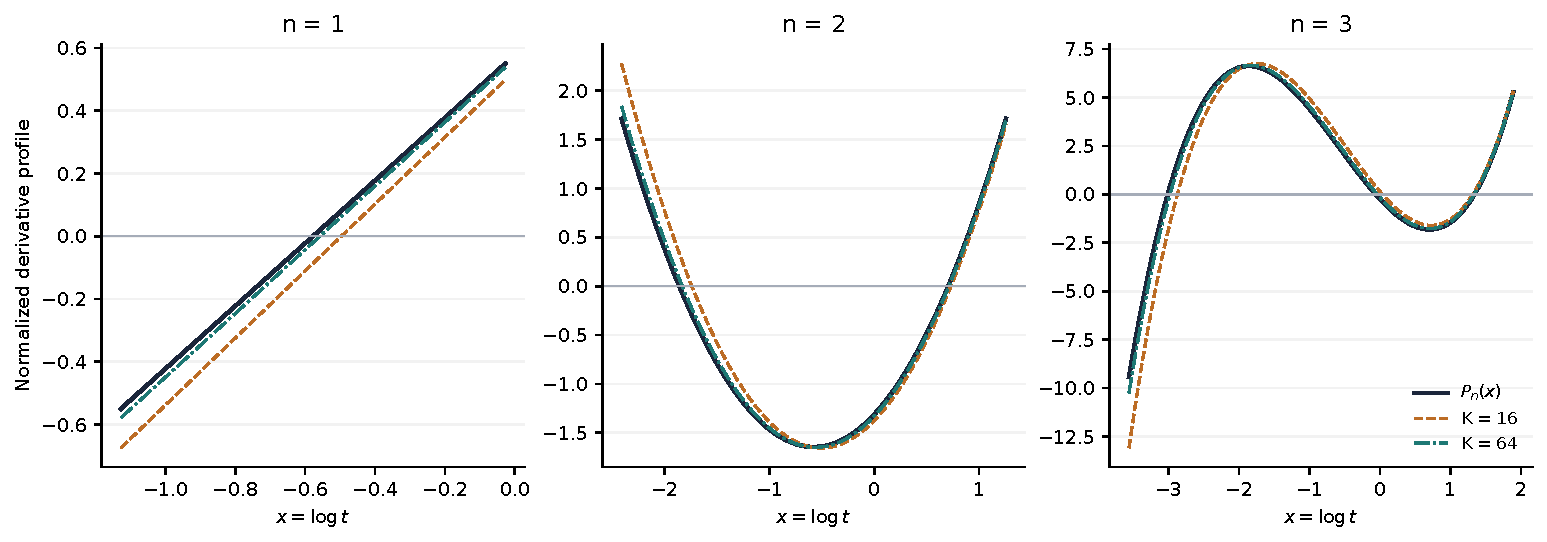
\includegraphics[width=0.98\linewidth]{../reports/corpus-corrections/figures/12-relation-spaces-stieltjes_profiles.pdf}
\caption{Normalized derivative profiles
$(1-e^{-e^x})\mathcal H_{n,K}(e^x)$ approach $P_n(x)$ as $K=k+1$
increases.  The plots illustrate $n=1,2,3$.  Quadrature produces the
curves; Theorems~\ref{zeros:thm:globalzeros} and \ref{zeros:thm:zeroasympt}, rather
than the plots, prove the zero counts and asymptotic completeness.}
\label{half:zero:profile-figure}
\end{figure}

\section{Exact low-index zero counts}
The general theorem proves eventual saturation. At the classical endpoint
$\rho=1$, a finite exact certificate supplies a stronger statement for
$1\le n\le4$ at every $k\ge1$.
Define the sign-preserving normalization
\[
\mathcal V_{n,k}(a)=\frac{a^{k+1}(-1)^{n+k}}{k!}\gamma_n^{(k)}(a).
\]
\subsection{A reproducible Euler--Maclaurin sign certificate}
The finite certificates above can be checked without floating-point special
functions. Put $p=k+1$, and define
\[
R_{n,\ell}(v)=n!\sum_{j=0}^n
 e_{n-j}(\ell)\frac{(-v)^j}{j!}.
\]
The master identity gives the absolutely convergent spectral representation
\[
\mathcal V_{n,k}(a)=\sum_{m\ge0}
 \left(\frac a{a+m}\right)^p R_{n,k}(\log(a+m)).
\]
For positive rational $a$, integers $M,R\ge1$, $A=a+M>1$ and $L=k+2R$,
let
\begin{align*}
\mathcal E_{M,R}={}&\sum_{m=0}^{M-1}
 \left(\frac a{a+m}\right)^p R_{n,k}(\log(a+m))\\
&+\left(\frac aA\right)^p\left[
 \frac Ak R_{n,k-1}(\log A)+\frac12R_{n,k}(\log A)\right]\\
&+\left(\frac aA\right)^p
 \sum_{r=1}^R\frac{B_{2r}}{(2r)!}
 \left(\prod_{j=1}^{2r-1}\frac{k+j}{A}\right)
 R_{n,k+2r-1}(\log A).
\end{align*}
\begin{proposition}[An explicit rational-certifiable remainder]
One has
\begin{align*}
\left|\mathcal V_{n,k}(a)-\mathcal E_{M,R}\right|
&\le\left(\frac aA\right)^p
 \frac{|B_{2R}|}{(2R)!}
 \left(\prod_{j=1}^{2R-1}\frac{k+j}{A}\right)
 \mathcal B_{n,L}(\log A),\\
\mathcal B_{n,L}(v)
&=\sum_{i=0}^{\min(n,L)}\sum_{j=0}^{n-i}
 \frac{n!e_i(L)}{(n-i-j)!L^j}v^{n-i-j}.
\end{align*}
Every factor in the bound is nonnegative.
\end{proposition}
\begin{proof}
Apply Euler--Maclaurin through the $R$th Bernoulli term to the spectral
sum, or equivalently apply it to the Hurwitz series before extracting the
$n$th spectral coefficient. The integral and half-endpoint terms give the
second line of $\mathcal E_{M,R}$. The identity
$(1+u)_k(k+1+u)_{2r-1}=(1+u)_{k+2r-1}$ gives its correction terms.

The periodic Bernoulli remainder has absolute kernel bound $|B_{2R}|$.
After differentiation, bound the absolute value of $R_{n,L}(\log t)$
by $n!\sum_i e_i(L)(\log t)^{n-i}/(n-i)!$ for $t\ge A>1$.
For each $d\ge0$,
\[
\int_A^\infty t^{-L-1}\log^d t\,dt
=\frac{A^{-L}}L\sum_{j=0}^d
 \frac{d!}{(d-j)!L^j}\log^{d-j}A.
\]
The last factor in $(k+1)_{2R}$ cancels the leading $L$ in this
integral. Substitution yields precisely the displayed bound.
\end{proof}

Logarithms of positive rationals have elementary rational enclosures.
Reduce their argument to $1\le y<2$ by a power of two, put
$u=(y-1)/(y+1)$, and use
\[
0\le\log y-2\sum_{j=0}^{T-1}\frac{u^{2j+1}}{2j+1}
\le\frac{2u^{2T+1}}{(2T+1)(1-u^2)}.
\]
The interval verifier uses integer endpoints scaled by $10^{90}$ and
rounds every operation outward. The Bernoulli numbers and $e_i(\ell)$
are exact rationals. A final enclosure lying strictly on one side of
zero is therefore a sign certificate; the proof of the analytic remainder
and the rational arithmetic play separate roles.

The fresh replay verified fourteen base signs for $n\le4$ and sixteen
endpoint signs isolating the unique $n=1$ roots for
$k=1,2,5,10,20,50,100,200$. The endpoint pairs have width $10^{-20}$.
These are global root certificates because the zero-count theorem proves
uniqueness, rather than merely sampled sign changes near a candidate root.


The following enclosures use integer interval arithmetic with outward
rounding, rational logarithm bounds and a proved Euler--Maclaurin remainder.
They have been replayed in this consolidation. The factor $a^{k+1}/k!$
is part of the tabulated value.
\begin{center}
\begin{tabular}{cclc}
\toprule
$n$ & $a$ & Certified enclosure for $\mathcal V_{n,1}(a)$ & Sign\\
\midrule
1 & $1$ & $[0.70738581,\ 0.70738582]$ & $+$\\
1 & $1.5$ & $[-0.20183770,\ -0.20183769]$ & $-$\\
2 & $1$ & $[0.11418372,\ 0.11418373]$ & $+$\\
2 & $1.3$ & $[-0.12008911,\ -0.12008910]$ & $-$\\
2 & $2$ & $[0.45673490,\ 0.45673491]$ & $+$\\
3 & $0.8$ & $[0.16385907,\ 0.16385908]$ & $+$\\
3 & $1.1$ & $[-0.04095264,\ -0.04095263]$ & $-$\\
3 & $1.5$ & $[0.05603756,\ 0.05603757]$ & $+$\\
3 & $2.1$ & $[-0.24542536,\ -0.24542535]$ & $-$\\
4 & $0.8$ & $[0.03897530,\ 0.03897531]$ & $+$\\
4 & $0.94$ & $[-0.00338878,\ -0.00338877]$ & $-$\\
4 & $1.2$ & $[0.02176370,\ 0.02176371]$ & $+$\\
4 & $1.7$ & $[-0.03656822,\ -0.03656821]$ & $-$\\
4 & $2.2$ & $[0.15091738,\ 0.15091739]$ & $+$\\
\bottomrule
\end{tabular}
\end{center}

\begin{corollary}[Saturation at every derivative order for $n\le4$]
For $1\le n\le4$ and every $k\ge1$, $\gamma_n^{(k)}$ has exactly $n$
positive zeros, all simple. They interlace to the right as $k$ increases.
\end{corollary}
\begin{proof}
At $k=1$ each row group gives $n$ sign-changing disjoint intervals, so
there are at least $n$ distinct zeros. The global bound with multiplicity
makes them the only zeros and makes each simple. Persistence and
interlacing follow from Corollary~\ref{zeros:cor:interlacing}.
\end{proof}
This finite certification does not settle every small-$k$ case for
$n\ge5$, and it does not assert saturation at every small order uniformly
in the Lerch deformation.

\section{High parameter derivatives of Stieltjes constants}
\label{spectral:sec:asymptotics}

The parameter-derivative tower admits a useful separation into a
finite polynomial coefficient and an exponentially small spectral
tail. This gives a different asymptotic regime from the frequently
studied limit of a large Stieltjes index with derivative order fixed.
Here the derivative order \(k\) tends to infinity, while the index
\(n\) may grow proportionally to \(\log k\). The resulting profile is
the reciprocal gamma function.

\subsection{An exact spectral expansion}

Fix the Laurent convention
\begin{equation}\label{spectral:eq:stieltjes-convention}
\zeta(s,a)=\frac{1}{s-1}
 +\sum_{n=0}^{\infty}\frac{(-1)^n}{n!}\gamma_n(a)(s-1)^n,
\qquad a>0.
\end{equation}
The superscript \(\gamma_n^{(k)}(a)\) always denotes differentiation
with respect to \(a\), not to the index or the zeta variable. Define
\begin{equation}\label{spectral:eq:coefficient-polynomial}
P_{n,k}(x)=n![z^n]\left(e^{xz}\prod_{j=1}^{k}
                  \left(1+\frac zj\right)\right).
\end{equation}
This is a degree-\(n\) polynomial in \(x\); its coefficients are
rational. In particular \(P_{0,k}=1\) and
\(P_{1,k}(x)=x+H_k\).

\begin{theorem}[Spectral expansion and a finite-tail certificate]
\label{spectral:thm:spectral}
For \(a>0\), integers \(k\ge1\), and \(n\ge0\),
\begin{equation}\label{spectral:eq:spectral}
\frac{(-1)^{n+k}}{k!}\gamma_n^{(k)}(a)
=\sum_{m=0}^{\infty}
 \frac{P_{n,k}(-\log(a+m))}{(a+m)^{k+1}}.
\end{equation}
The series converges absolutely, locally uniformly for \(a>0\).
If the sum is truncated before \(m=M\), where \(b=a+M\ge1\),
then for every real \(0<R<k\) the magnitude of the omitted part is at
most
\begin{equation}\label{spectral:eq:spectral-tail}
\frac{n!}{R^n}\prod_{j=1}^{k}\left(1+\frac Rj\right)
\left(b^{-k-1+R}+\frac{b^{-k+R}}{k-R}\right).
\end{equation}
\end{theorem}

\begin{proof}
The Hurwitz-zeta parameter identity
\[
\partial_a^k\zeta(s,a)=(-1)^k(s)_k\zeta(s+k,a)
\]
follows initially by differentiating its absolutely convergent
Dirichlet series and then by analytic continuation; here
\((s)_k=s(s+1)\cdots(s+k-1)\).
The pole in \eqref{spectral:eq:stieltjes-convention} is independent of \(a\).
Put \(s=1+z\), use
\((1+z)_k=k!\prod_{j=1}^k(1+z/j)\), and compare coefficients.
For \(|z|<k\), the series for \(\zeta(k+1+z,a)\) converges normally.
This gives \eqref{spectral:eq:spectral} and justifies the coefficient
interchange. Alternatively, absolute convergence follows directly
because each summand is a linear combination of
\((a+m)^{-k-1}\log^\ell(a+m)\), \(0\le\ell\le n\).
The parameter identity is also the starting point of
Coffey's all-order formulas~\cite{stieltjes:Coffey}.

On the circle \(|z|=R\), and for \(x\ge b\ge1\),
\[
\left|e^{-z\log x}\prod_{j=1}^k(1+z/j)\right|
\le x^R\prod_{j=1}^k(1+R/j).
\]
Cauchy's coefficient estimate bounds the \(m\)-th omitted summand
by \(n!R^{-n}\prod_j(1+R/j)(a+m)^{-k-1+R}\).
For the positive decreasing power, comparison with its integral gives
\[
\sum_{m=M}^{\infty}(a+m)^{-k-1+R}
\le b^{-k-1+R}+\int_b^\infty x^{-k-1+R}\,dx.
\]
This is \eqref{spectral:eq:spectral-tail}.
\end{proof}

The condition \(b\ge1\) belongs to the stated majorant, rather than to
the exact expansion. It always holds for the tail after the first
term, because then \(b=a+1>1\). The choice of \(R\) can be optimized
for a given \(n,k,M\); there is no need to differentiate a
highly oscillatory numerical representation of \(\gamma_n\).

\subsection{Exact rational enclosures at parameter one}

Write \(\stirling{v}{u}\) for the unsigned Stirling number of the
first kind. The elementary identity
\begin{equation}\label{spectral:eq:stirling-product}
\prod_{j=1}^k(1+z/j)
 =\frac1{k!}\sum_{n=0}^k\stirling{k+1}{n+1}z^n
\end{equation}
turns the first spectral term at \(a=1\) into an exact rational
number.

\begin{corollary}[Rational certificates]\label{spectral:cor:rational}
Let \(k\ge2\), \(n\ge0\), and
\[
e_n(k)=
\begin{cases}
\stirling{k+1}{n+1}/k!,&0\le n\le k,\\
0,&n>k.
\end{cases}
\]
For any integer \(1\le h<k\), set
\begin{equation}\label{spectral:eq:rational-radius}
B_{k,n,h}
=h^{-n}\binom{k+h}{h}
 \left(2^{-k-1+h}+\frac{2^{-k+h}}{k-h}\right).
\end{equation}
Then the following is an exact inclusion between real numbers:
\begin{equation}\label{spectral:eq:rational-inclusion}
\frac{(-1)^{n+k}\gamma_n^{(k)}(1)}{k!\,n!}
\in[e_n(k)-B_{k,n,h},\,e_n(k)+B_{k,n,h}].
\end{equation}
One may take the minimum radius over all \(h=1,\ldots,k-1\).
In particular, the simple choice \(h=1\) gives
\begin{equation}\label{spectral:eq:simple-rational-radius}
B_k=(k+1)\left(2^{-k}+\frac{2^{-k+1}}{k-1}\right),
\end{equation}
independently of \(n\).
\end{corollary}

\begin{proof}
Apply Theorem~\ref{spectral:thm:spectral} with \(a=M=1\), \(b=2\), and
\(R=h\), and divide its bound by \(n!\). The product in that bound is
\(\prod_{j=1}^k(1+h/j)=\binom{k+h}{h}\).
Equation~\eqref{spectral:eq:stirling-product} supplies the center.
All quantities in the resulting endpoints are rational.
\end{proof}

Thus the term \emph{certificate} has its literal meaning here:
integer arithmetic constructs the endpoints, and the proved tail
bound supplies the inclusion. Floating-point agreement is not being
renamed a proof. For example, positivity of an endpoint
\(e_n(k)-B_{k,n,h}\) rigorously proves
\((-1)^{n+k}\gamma_n^{(k)}(1)>0\).
The accompanying script emits centers, radii, and both endpoints
as numerator--denominator pairs, and checks their arithmetic exactly.

\subsection{A uniform coefficient lemma}

The main asymptotic step is an elementary coefficient estimate.
It is convenient to set
\(\fall{n}{j}=n(n-1)\cdots(n-j+1)\) for \(j\le n\), and
\(\fall{n}{j}=0\) for \(j>n\).

\begin{lemma}[Two uniform coefficient terms]\label{spectral:lem:coefficient}
Suppose \(f\) is analytic on a neighborhood of the closed disk
\(|z|\le R\), with \(|f(z)|\le M\) there. Let \(L>0\),
\(n\ge1\), and \(r=n/L<R\). Put
\[
Q_n(L;f)=\frac{n!}{L^n}[z^n]e^{Lz}f(z).
\]
Then
\begin{align}
|Q_n(L;f)-f(r)|
&\le\frac{Mn}{L^2R^2(1-r/R)^3},\label{spectral:eq:coefficient-first}\\
\left|Q_n(L;f)-f(r)+\frac{n}{2L^2}f''(r)\right|
&\le\frac{3Mn}{L^3R^3(1-r/R)^5}.\label{spectral:eq:coefficient-second}
\end{align}
For \(n=0\), \(Q_0(L;f)=f(0)\) exactly.
\end{lemma}

\begin{proof}
Write \(f(z)=\sum_{j\ge0}c_jz^j\). Since \(|c_j|\le MR^{-j}\),
\[
Q_n(L;f)=\sum_{j\ge0}c_j\frac{\fall{n}{j}}{L^j}
\]
is a finite sum, which we compare with the absolutely convergent
Taylor series at \(r\).

For completeness, the needed inequalities remain valid when \(j>n\).
Choose \(j\) independent uniform elements of a set of \(n\) elements.
The probability of no repeated choice is
\(\fall{n}{j}/n^j\), including its value zero when \(j>n\).
For the \(K=\binom j2\) pair-collision events, every event has
probability \(1/n\), and every intersection of two distinct events
has probability \(1/n^2\), even if the pairs share a position.
The union bound and the first two Bonferroni inequalities give
\begin{align*}
0&\le n^j-\fall{n}{j}\le\binom j2 n^{j-1},\\
0&\le\fall{n}{j}-n^j+\binom j2 n^{j-1}
 \le\binom{\binom j2}{2}n^{j-2}.
\end{align*}
At \(j=0,1,2\), the second remainder is zero, so no negative-power
exception is needed. Now use
\[
\sum_{j\ge2}\binom j2 x^{j-2}=(1-x)^{-3},
\qquad
\sum_{j\ge3}\binom{\binom j2}{2}x^{j-3}=3(1-x)^{-5}.
\]
The first inequality gives \eqref{spectral:eq:coefficient-first}.
In the second comparison,
\[
\sum_{j\ge2}c_j\binom j2\frac{n^{j-1}}{L^j}
=\frac{n}{2L^2}f''(r).
\]
This proves \eqref{spectral:eq:coefficient-second}.
\end{proof}

\subsection{The reciprocal-gamma profile}

\begin{theorem}[A joint logarithmic-range asymptotic]\label{spectral:thm:profile}
Fix \(0<a_0\le a_1<\infty\) and \(C>0\). For
\(a\in[a_0,a_1]\), put
\[
L=\log(k/a),\qquad r=\frac nL,\qquad
g(r)=\frac1{\Gamma(1+r)},\qquad
\rho=\frac{a_1}{a_1+1}<1.
\]
Uniformly over integers \(0\le n\le CL\), as \(k\to\infty\),
\begin{equation}\label{spectral:eq:uniform-profile}
\frac{(-1)^{n+k}a^{k+1}\gamma_n^{(k)}(a)}{k!\,L^n}
=g(r)-\frac{n}{2L^2}g''(r)
 +O_{a_0,a_1,C}\left(\frac n{L^3}+k^{C+1}\rho^k\right).
\end{equation}
Equivalently, the two displayed terms are
\begin{equation}\label{spectral:eq:profile-polygamma}
\frac1{\Gamma(1+r)}
\left[1+\frac{n}{2L^2}
 \left\{\psi^{(1)}(1+r)-\psi(1+r)^2\right\}\right].
\end{equation}
The formula includes \(n=0\), for which the first spectral term is
exactly one. In particular, if \(n/\log(k/a)\to c\ge0\) in a bounded
range, then the left side of \eqref{spectral:eq:uniform-profile} tends to
\(1/\Gamma(1+c)\).
\end{theorem}

\begin{proof}
Separate the \(m=0\) term of \eqref{spectral:eq:spectral}. Its generating
function factors as
\[
e^{-z\log a}\prod_{j=1}^k(1+z/j)=e^{Lz}f_k(z),
\qquad
f_k(z)=k^{-z}\prod_{j=1}^k(1+z/j).
\]
The gamma product gives
\[
f_k(z)=\frac{\Gamma(k+1+z)}
 {\Gamma(k+1)k^z\Gamma(1+z)}
      =g(z)e^{D_k(z)}.
\]
On \(|z|<k+1\), define the analytic function
\begin{equation}\label{spectral:eq:Dk}
D_k(z)=z(H_k-\log k-\gamma)
 +\sum_{\ell=2}^{\infty}
   \frac{(-1)^\ell z^\ell}{\ell}
       \bigl(\zeta(\ell)-H_k^{(\ell)}\bigr).
\end{equation}
The factorization follows first on a small disk from the
Weierstrass product and then throughout \(|z|<k+1\) by analytic
continuation. Defining \(D_k\) by its series avoids taking the
logarithm of \(g\) at its zeros.

The elementary bounds
\[
0<H_k-\log k-\gamma<\frac1{2k},\qquad
\sum_{j>k}j^{-2}\le\frac1k
\]
imply, for \(|z|\le R<k+1\),
\begin{equation}\label{spectral:eq:Dk-bound}
|D_k(z)|\le\frac{R}{2k}
   +\frac{R^2}{2k(1-R/(k+1))}.
\end{equation}
Indeed, for \(\ell\ge2\), bound the tail of \(\zeta(\ell)\) by
\((k+1)^{2-\ell}/k\), and use \(1/\ell\le1/2\).
Consequently \(f_k\) is uniformly bounded on every fixed disk,
\(f_k-g=O_R(k^{-1})\), and Cauchy's estimate gives
\(f_k''-g''=O_C(k^{-1})\) on \([0,C]\).
The same estimate with \(R=r\), or the real product, also gives the
slightly sharper
\[
f_k(r)-g(r)=O_C(r/k)\qquad(0\le r\le C).
\]
It is this factor \(r\) that preserves the exact \(n=0\) first term.

Choose \(R=C+1\) in Lemma~\ref{spectral:lem:coefficient}. For \(n\ge1\)
the normalized first spectral term is
\[
Q_n(L;f_k)
=f_k(r)-\frac{n}{2L^2}f_k''(r)+O_C(n/L^3).
\]
Replacing \(f_k\) by \(g\) costs
\(O_C(n/(kL)+n/(kL^2))\), which is absorbed in \(O(n/L^3)\)
because \(L^2\le k\) for all sufficiently large \(k\), uniformly
on the compact parameter interval.

It remains to control the other spectral terms. Apply
\eqref{spectral:eq:spectral-tail} with \(M=1\), and multiply the bound by
\(a^{k+1}/L^n\). The result is
\[
\frac{n!}{(RL)^n}\prod_{j=1}^k(1+R/j)
\left(\frac{a}{a+1}\right)^{k+1}(a+1)^R
\left(1+\frac{a+1}{k-R}\right).
\]
The first factor is at most one: for \(n\ge1\), use
\(n!\le n^n\) and \(n/L\le C<R\); for \(n=0\), it is one by
convention. The product is \(O_R(k^R)\), as follows already from
\eqref{spectral:eq:Dk-bound} at \(z=R\).
The remaining factors are uniformly bounded apart from
\((a/(a+1))^{k+1}\le\rho^{k+1}\). Thus the normalized tail is
\(O_{a_0,a_1,C}(k^{C+1}\rho^k)\). The case \(n=0\) follows
directly from \(P_{0,k}=1\).
Finally,
\(g''(r)=g(r)\{\psi(1+r)^2-\psi^{(1)}(1+r)\}\).
\end{proof}

\begin{corollary}[A uniform eventual sign]\label{spectral:cor:sign}
For every compact interval \([a_0,a_1]\subset(0,\infty)\) and
every \(C>0\), there is \(k_0\) such that
\[
(-1)^{n+k}\gamma_n^{(k)}(a)>0
\]
for all \(k\ge k_0\), \(a\in[a_0,a_1]\), and integers
\(0\le n\le C\log(k/a)\).
\end{corollary}

\begin{proof}
The continuous function \(g\) is strictly positive on \([0,C]\),
so its minimum there is positive. Both the displayed correction
and the remainder in Theorem~\ref{spectral:thm:profile} tend uniformly to zero.
The other factors in the normalization are positive.
\end{proof}

The corollary is restricted to its stated range. It gives no sign
theorem when \(n\) grows arbitrarily quickly compared with \(\log k\).
For a concrete finite pair \(n,k\) at \(a=1\), the rational interval
in Corollary~\ref{spectral:cor:rational} is a separate, effective certificate.

\begin{figure}[tbp]
\centering
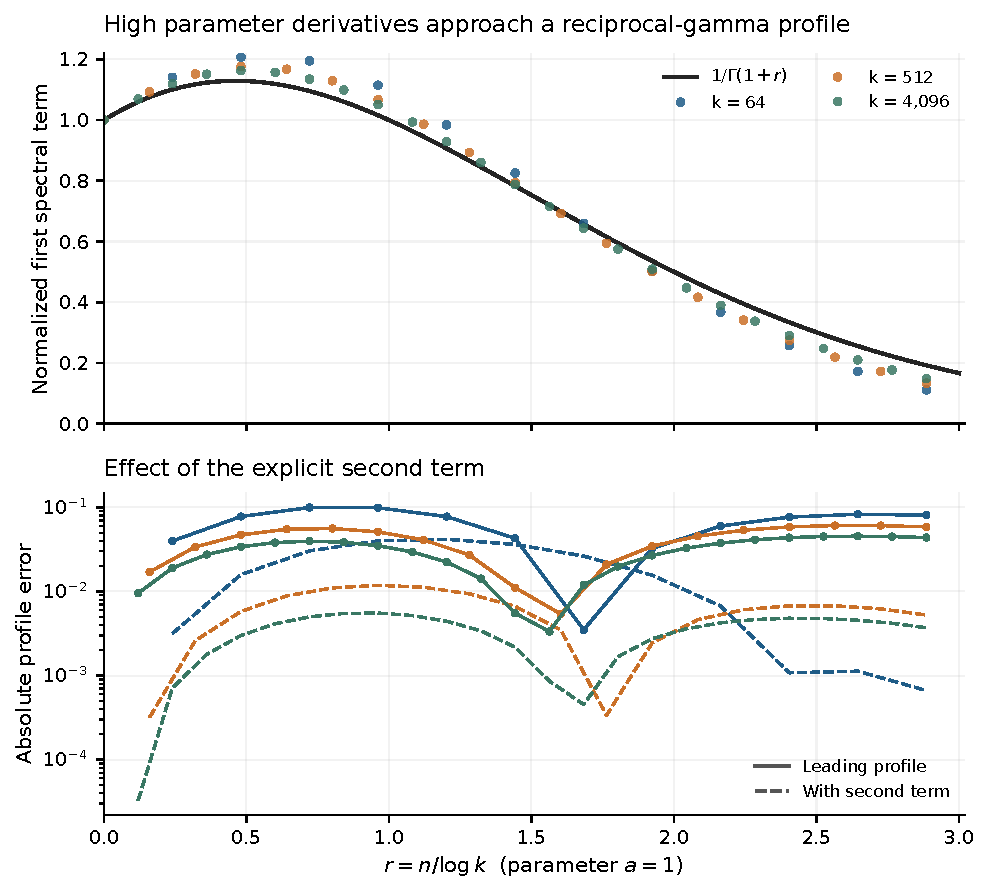
\includegraphics[width=\textwidth]{../reports/rational-grid-distribution-ranks/figures/10-exact-structure-derivative-profile.pdf}
\caption{The reciprocal-gamma profile at \(a=1\).
The first spectral term is computed from the elementary-symmetric
coefficient recurrence; its rigorously bounded spectral error is
smaller than the plotted resolution.
The lower panel compares its deviation from the limiting profile
with its deviation after the explicit second term is included.
These plotted arithmetic evaluations are floating point; the separate
rational certificates do not depend on them.}
\label{spectral:fig:profile}
\end{figure}

\subsection{Fixed-index expansions and the classical mechanism}

For a fixed \(n\), it is also useful to retain the polynomial in
\(L=\log(k/a)\). Define Appell polynomials
\[
A_n(L)=n![z^n]\frac{e^{Lz}}{\Gamma(1+z)}.
\]
The first few are
\begin{align*}
A_0(L)&=1,\\
A_1(L)&=L+\gamma,\\
A_2(L)&=(L+\gamma)^2-\zeta(2),\\
A_3(L)&=(L+\gamma)^3-3\zeta(2)(L+\gamma)+2\zeta(3).
\end{align*}
The standard gamma-ratio expansion~\cite{hstruct:DLMF} gives, uniformly on
fixed \(z\)-disks,
\[
e^{D_k(z)}=
1+\frac{z+z^2}{2k}
 +\frac{3z^4+2z^3-3z^2-2z}{24k^2}+O(k^{-3}).
\]
Consequently, for fixed \(n\ge1\) and \(a\) in a compact positive
interval,
\begin{align}
\frac{(-1)^{n+k}a^{k+1}\gamma_n^{(k)}(a)}{k!}
={}&A_n(L)
 +\frac{nA_{n-1}(L)+n(n-1)A_{n-2}(L)}{2k}\notag\\
&+O_n\left(\frac{(1+L)^{n-1}}{k^2}\right)
 +O_{a_0,a_1,n}(k^2\rho^k).
\label{spectral:eq:fixed-index}
\end{align}
Terms with a negative Appell index are omitted.
To see the stated polynomial error, note that the analytic
remainder after the first correction vanishes at \(z=0\);
its coefficient convolution with \(e^{Lz}g(z)\) therefore has
degree at most \(n-1\) in \(L\). For \(n=0\) the first term is
exact and only the spectral error remains.
Higher powers of \(k^{-1}\) follow by the same coefficient procedure.
For example the \(k^{-2}\) numerator is
\[
\frac1{24}\left(
3\fall{n}{4}A_{n-4}
+2\fall{n}{3}A_{n-3}
-3\fall{n}{2}A_{n-2}
-2nA_{n-1}\right).
\]

At \(a=1\), \eqref{spectral:eq:stirling-product} identifies the first spectral
term with first-kind Stirling numbers. These are also the cycle-count
coefficients of permutations. The reciprocal-gamma factor is thus a
classical mechanism, closely related to mod-Poisson asymptotics
\cite{spectral:KowalskiNikeghbali}. The contribution to this programme is the
explicit spectral transfer, the uniform second coefficient estimate,
and the exact rational enclosure, not a claim that the
reciprocal-gamma phenomenon itself is new.

\chapter{Herglotz arithmetic and quadratic regulators}
\label{ch:09-herglotz}

The Herglotz function joins the digamma series to finite dilogarithm sums.
At rational arguments this supplies exact evaluations; at quadratic units it
connects continued-fraction cycles with real-quadratic Kronecker limits.
The same experimental strategy thus leads from a finite cyclotomic sum to
regulator candidates in class fields.

\section{The function and the exact dilogarithm sum}
For $x>0$ define
\[
F(x)=\sum_{n\ge1}\frac{\psi(nx)-\log(nx)}n,
\qquad
J(x)=\int_0^1\frac{\log(1+t^x)}{1+t}\,dt.
\]
The series is locally uniformly convergent on the positive line and extends
analytically to the cut plane $\mathbb C\setminus(-\infty,0]$.
Radchenko--Zagier relate the two functions by

\begin{equation}\label{herg:eq:Jint}
  J(x)=\int_0^1\frac{\log(1+t^{x})}{1+t}\,dt,\qquad J(x)=F(2x)-2F(x)+F(x/2)+\frac{\pi^2}{12x},
\end{equation}
which relates the companion $J$ to the Herglotz function $F$. For the rational-argument results the engine is
Radchenko--Zagier's Theorem~3, an \emph{exact, finite} evaluation obtained from the second integral
representation of $F$ via the distribution relations:
\begin{equation}\label{herg:eq:dilogsum}
  F\!\Bigl(\tfrac PQ\Bigr)-F(1)=\sum_{\alpha^P=1}\Bigl(\sum_{\substack{\beta^Q=1\\\beta\neq1}}f(\alpha,\beta)
  -\sum_{\substack{\beta^P=1\\\beta\neq1}}f(\alpha,\beta)\Bigr),\quad
  f(\alpha,\beta)=\Li_2\!\Bigl(\tfrac{\beta}{\beta-1}\Bigr)-\Li_2\!\Bigl(\tfrac{\alpha-\beta}{1-\beta}\Bigr).
\end{equation}
The finite sum is an exact analytic identity, with compatible principal
branches at its arguments. Floating-point evaluation still has rounding
and cancellation errors. It is a useful independent comparator for the
defining integral, not a zero-error numerical oracle.

\section{Quadratic-unit values: Tables 1 \& 2, and two errata}\label{herg:sec:tables}
For real quadratic units the relevant object is the companion
$\Jcal(x)=J(x)-\tfrac{\log^2 2}{2}+\tfrac{\pi^2}{24}(x-\tfrac1x)$, and the arithmetic atoms are
$S_{p,q}=\log\eps_p\,\log\eps_q$ where $\eps_d$ is the fundamental unit of $\mathbb Q(\sqrt d)$ for a
fundamental discriminant $d>1$ and $\eps_1:=2$. Tables~1 and~2 of the source paper express, for the $45$
known one-class-per-genus cases, the quantities
$4\bigl(\Jcal(n+\sqrt{n^2-1})-n\tfrac{\pi^2}{24}\bigr)$ and
$2\bigl(\Jcal(n+\sqrt{n^2+1})-n\tfrac{\pi^2}{24}\bigr)$ as integer combinations of the $S_{p,q}$.

We re-implemented $\Jcal$ and $S_{p,q}$ in PARI/GP (\texttt{intnum} integrals, \texttt{bnfinit} regulators)
and evaluated both sides of all $45$ rows at $200$-digit precision. All $16$ rows of Table~2 and $27$ of the
$29$ rows of Table~1 agree to better than $10^{-80}$. The two failures are $O(1)$:
\[
  \text{$n=43$:}\ \ \text{LHS}-\text{RHS}=-13.0160\ldots,\qquad
  \text{$n=61$:}\ \ \text{LHS}-\text{RHS}=-2.9011\ldots .
\]
Each resolves to a single exact correction, confirmed against the high-DPI scan to be a typo in the printed
paper rather than an OCR artifact.

\begin{proposition}[Two corrections to Table 1]
\leavevmode
\begin{itemize}[topsep=2pt,itemsep=1pt]
\item $n=43$ ($n^2-1=2^3\cdot3\cdot7\cdot11$): the printed right-hand side overshoots by exactly $S_{33,56}$
$\bigl((\text{LHS}-\text{RHS})/S_{33,56}=-1.000\ldots$ to $110$ digits$\bigr)$; the spurious $+S_{33,56}$
term should be deleted.
\item $n=61$ ($n^2-1=2^3\cdot3\cdot5\cdot31$): the printed $S_{60,1032}$ should read $S_{60,248}$. The
printed subscript $1032=2^3\cdot3\cdot43$ carries the prime $43$, foreign to $n^2-1=3720$, whereas
$60\cdot248=14880=4\cdot3720$ is the correct genus splitting.
\end{itemize}
A brute-force search over all single edits (delete a term, change a coefficient in $[-4,4]$, or replace a
subscript by any admissible fundamental-discriminant pair) returns these as the \emph{unique} fixes. With
both applied, all $45$ rows verify to better than $10^{-80}$.
\end{proposition}

The quadratic-unit tables concern specified arithmetic families. They do
not imply that every even-trace unit has a pure-logarithm evaluation:
outside genus characters the Kronecker-limit formula introduces additional
class-group coordinates. Those coordinates are developed below.

\section{Rational arguments: a family of theorems}\label{herg:sec:rational}
The paper writes out only two rational-argument cases: $F(n)$ (pure logarithms, its eq.~23) and the lone
fractional example $F(2/5)$ (its eq.~24). We now give the general laws.

\subsection{Two reductions on the line \texorpdfstring{$\Real=\tfrac12$}{Re=1/2}}
Everything rests on one observation: for a unit $\beta=e^{i\theta}$,
\begin{equation}\label{herg:eq:line}
  \frac{\beta}{\beta-1}\ \text{has real part}\ \tfrac12,\qquad
  \arg\frac{\beta}{\beta-1}=\frac{\theta}{2}-\frac{\pi}{2},\qquad
  \Bigl|\frac{\beta}{\beta-1}\Bigr|=\frac{1}{2\sin(\theta/2)} .
\end{equation}
By the reflection $\Li_2(z)+\Li_2(1-z)=\tfrac{\pi^2}{6}-\log z\log(1-z)$ with $1-z=\bar z$ on $\Real z=\tfrac12$,
\begin{equation}\label{herg:eq:reRe}
  2\Real\Li_2\Bigl(\tfrac12+iy\Bigr)=\frac{\pi^2}{6}-\log^2|z|-(\arg z)^2 .
\end{equation}
The second reduction handles the $\alpha=-1$ part of~\eqref{herg:eq:dilogsum}: $\tfrac{-1-\beta}{1-\beta}=-i\cot\tfrac\theta2$
is purely imaginary, and for real $y$
\begin{equation}\label{herg:eq:imax}
  \Real\Li_2(iy)=\tfrac14\Li_2(-y^2).
\end{equation}

\subsection{$F(1/q)$: pure logarithms}
\begin{theorem}\label{herg:thm:F1q}
For all $q\ge2$, with $m=\lfloor(q-1)/2\rfloor$,
\[
  F\!\Bigl(\tfrac1q\Bigr)-F(1)=-\frac{(q-1)(3q-2)}{24q}\,\pi^2
  -\sum_{k=1}^{m}\log^2\!\Bigl(2\sin\tfrac{\pi k}{q}\Bigr)\;-\;[\,q\ \mathrm{even}\,]\,\tfrac12\log^2 2 .
\]
\end{theorem}
\begin{proof}
With $P=1$ only $\alpha=1$ occurs and the inner $\beta^P$-sum is empty, so~\eqref{herg:eq:dilogsum} reads
$F(1/q)-F(1)=\sum_{\beta^q=1,\beta\neq1}(\Li_2(\tfrac{\beta}{\beta-1})-\tfrac{\pi^2}{6})$. Pairing $\beta$ with
$\bar\beta$ and applying~\eqref{herg:eq:reRe} gives the $\pi^2$ coefficient
$-\bigl[\tfrac{q-1}{12}+\sum_{k=1}^m(\tfrac kq-\tfrac12)^2\bigr]=-\tfrac{(q-1)(3q-2)}{24q}$ and the log-sine sum.
For even $q$ the self-conjugate root $\beta=-1$ contributes $\Li_2(\tfrac12)=\tfrac{\pi^2}{12}-\tfrac12\log^2 2$.
\end{proof}

\subsection{$F(2/q)$: the general theorem}
\begin{theorem}\label{herg:thm:F2q}
For every $q\ge3$,
\[
  F\!\Bigl(\tfrac2q\Bigr)-F(1)=-\frac{(q-1)(q-2)}{12q}\pi^2+\log^2 2
  -2\!\!\sum_{k=1}^{\lfloor(q-1)/2\rfloor}\!\!\log^2\!\Bigl(2\sin\tfrac{\pi k}{q}\Bigr)
  -\tfrac12\!\!\sum_{k=1}^{\lfloor(q-1)/2\rfloor}\!\!\Li_2\!\Bigl(-\cot^2\tfrac{\pi k}{q}\Bigr),
\]
where for even $q$ the two sums run to $k=\tfrac q2-1$ and a further $-\log^2 2$ is added.
\end{theorem}
\begin{proof}[Proof (odd $q$)]
Here $\alpha\in\{1,-1\}$ and the inner $\beta^P$-sum is the single term $\beta=-1$. For the first part,
$f(1,\beta)+f(-1,\beta)=2\Li_2(\tfrac{\beta}{\beta-1})-\tfrac{\pi^2}{6}-\Li_2(\tfrac{-1-\beta}{1-\beta})$.
Summing over $\beta\neq1$ and using~\eqref{herg:eq:reRe} for the first pieces and~\eqref{herg:eq:imax}
(with $\tfrac{-1-\beta}{1-\beta}=-i\cot\tfrac{\pi k}q$, pairing $k\leftrightarrow q-k$) for the last gives
$2S_1-(q-1)\tfrac{\pi^2}{6}-\tfrac12\sum_{k}\Li_2(-\cot^2\tfrac{\pi k}q)$, where
$S_1=\sum_{k=1}^{(q-1)/2}[\tfrac{\pi^2}{6}-\log^2(2\sin\tfrac{\pi k}q)-\pi^2(\tfrac kq-\tfrac12)^2]$. The boundary
gives $-\sum_\alpha f(\alpha,-1)=+\log^2 2$ from $\Li_2(\tfrac12)$. Collecting, the $\tfrac{\pi^2}{6}$ terms
cancel and the $\pi^2$ coefficient is $-2\sum_{k=1}^{(q-1)/2}(\tfrac kq-\tfrac12)^2$, which equals
$-\tfrac{(q-1)(q-2)}{12q}$ by an elementary identity (verified symbolically). The even-$q$ case differs only
in that $\beta=-1$ is now a genuine $q$-th root, contributing the extra $-\log^2 2$.
\end{proof}
The algebraic dilogarithm arguments make the field structure explicit.
At $q=5$ the symmetric sum can be reduced further as described below.
Unsuccessful searches at larger conductors do not prove that no other
closed form exists; the finite-sum theorem remains valid at every $q$.

\subsection{The $F(n/(n+1))$ family and the $F(p/2)$ reciprocity}
\begin{theorem}\label{herg:thm:np1}
For all $n\ge2$, with $S(q)=\sum_{k=1}^{q-1}\log^2(2\sin\tfrac{\pi k}q)$,
\[
  F\!\Bigl(\tfrac{n}{n+1}\Bigr)-F(1)=-\frac{3n^2+3n+2}{24n(n+1)}\pi^2+\Li_2\!\Bigl(\tfrac{n}{n+1}\Bigr)
  +\tfrac12\log^2\!\tfrac{n+1}{n}-\tfrac12 S(n+1)+\tfrac12 S(n),
\]
the single dilogarithm $\Li_2(n/(n+1))$ appearing with coefficient exactly $+1$ (the source paper's
``bilinear-log'' Example~2, made explicit). The $\pi^2$ coefficient equals $-\tfrac18-\tfrac1{12n(n+1)}$.
\end{theorem}
\begin{theorem}[Reciprocity]\label{herg:thm:p2}
For all odd $p\ge3$,
\[
  F\!\Bigl(\tfrac p2\Bigr)+F\!\Bigl(\tfrac2p\Bigr)-2F(1)=-\frac{(p-2)^2}{12p}\pi^2+\tfrac12\log^2\!\tfrac p2 .
\]
The $\Li_2(-\cot^2\frac{\pi k}{p})$ terms of $F(p/2)$ are exactly minus those of $F(2/p)$ and cancel in the
sum; combined with Theorem~\ref{herg:thm:F2q} this yields $F(p/2)$ in closed form.
\end{theorem}

\subsection{The derivative law}
\begin{theorem}[Radchenko--Zagier Proposition 4, $P=2$]\label{herg:thm:deriv}
For all $q\ge3$, with $T(q):=\tfrac2q F'(2/q)-(1+\log2)$,
\[
  T(q)=\frac{q^2-4}{24q}\pi^2+W(q),\qquad
  W(q)=\sum_{k=1}^{q-1}C(2k/q)\,\Cl_2\!\Bigl(\tfrac{2\pi k}q\Bigr),
\]
where $C(t)=\cot(\pi t)$ for $t\notin\mathbb Z$ and $C(t)=0$ for
$t\in\mathbb Z$, with an extra $-\log2$ for even $q$.
This assigned value at integers is part of the formula; a literal cotangent
there would be undefined. The sum provides a Clausen representation,
without an independence assertion.
\end{theorem}

\subsection{Rational-argument samples and the companion integral}
The source's proposed criterion $\operatorname{rad}(q)\mid30$ is false
as a necessary condition for a reduction to rational dilogarithms:
Theorem~\ref{herg:thm:F1q} gives a pure-logarithm answer for $F(1/7)$.
Numerator, denominator and the available functional equations must all be
considered. No replacement universal classification is asserted here.
The following experimentally recovered samples are useful:
\begin{align*}
F(3/4)-F(1)&=-\frac{19}{144}\pi^2-\frac34\log^22
-2\log2\log3+\frac74\log^23+2\Li_2(1/3),\\
F(4/5)-F(1)&=\frac3{80}\pi^2+\frac{11}4\log^22-\frac12\log^25
-\Li_2(1/5)-\log^2(2\sin(\pi/5))-\log^2(2\sin(2\pi/5)),\\
J(2/3)&=-\frac{\pi^2}{144}+\frac34\log^22,\\
J(2/5)&=\frac{11\pi^2}{240}+\frac34\log^22-2\log^2\phi.
\end{align*}
The last two values follow by combining the $F$ evaluations through
\eqref{herg:eq:Jint}. Their existence does not prove that these are the
only $q$ for which $J(2/q)$ simplifies.

\section{Bridges to the golden ladders and the Clausen lattice}\label{herg:sec:bridges}
The new constants are not isolated; they touch two corpora we have already mapped.

\paragraph{The golden bridge ($q=5$).} The arguments $-\cot^2\tfrac\pi5=-\tfrac{5+2\sqrt5}5$ and
$-\cot^2\tfrac{2\pi}5=-\tfrac{5-2\sqrt5}5$ lie in $\mathbb Q(\sqrt5)$, the field of the golden polylogarithm
ladders. Comparing Theorem~\ref{herg:thm:F2q} ($q=5$) with eq.~24 gives the functional equation
\[
  \Li_2\!\Bigl(\tfrac45\Bigr)+\Li_2\!\Bigl(-\cot^2\tfrac{\pi}{5}\Bigr)+\Li_2\!\Bigl(-\cot^2\tfrac{2\pi}{5}\Bigr)
  =2\log^2 2-2\log2\log\tfrac25-6\bigl(\log^2(2\sin\tfrac\pi5)+\log^2(2\sin\tfrac{2\pi}5)\bigr),
\]
hence the golden-sum closed form (with $\varphi=\tfrac{1+\sqrt5}2$)
\[
  \Li_2\!\Bigl(-\cot^2\tfrac{\pi}{5}\Bigr)+\Li_2\!\Bigl(-\cot^2\tfrac{2\pi}{5}\Bigr)
  =\Li_2\!\Bigl(\tfrac15\Bigr)-\frac{\pi^2}{6}-3\log^2\varphi+\tfrac14\log^2 5 .
\]
The symmetric sum has the displayed reduction. The antisymmetric
combination $X=\frac12[\Li_2(-\cot^2(\pi/5))-
\Li_2(-\cot^2(2\pi/5))]$ did not reduce in the source's tested basket.
Its independence is open. A formal symbol with nonzero Bloch boundary
is not subject to a vanishing-rank conclusion for the Bloch group.

\paragraph{The Clausen bridge.}
The coefficients of $W(q)$ are real algebraic numbers contained in
$\mathbb Q(\zeta_{\operatorname{lcm}(4,q)})^+$; at odd conductors the factor
$i$ implicit in the cotangent can require an extension of
$\mathbb Q(\zeta_q)^+$. This is an algebraic coefficient issue, not a proof
of numerical period independence. Applying the distribution identities
of Chapter~\ref{ch:02-cyclotomic} gives
\[
W(8)=2\Cl_2(\pi/4)-2\Cl_2(3\pi/4)=G,
\qquad
W(12)=\frac{11\sqrt3}{9}\Cl_2(\pi/3).
\]
For the second formula, pair $k$ with $12-k$:
\[
W(12)=2\sqrt3\left[\Cl_2(\pi/6)-\Cl_2(5\pi/6)\right]
+\frac2{\sqrt3}\left[\Cl_2(\pi/3)-\Cl_2(2\pi/3)\right].
\]
Use $\Cl_2(\pi/6)-\Cl_2(5\pi/6)=V/2$ and
$\Cl_2(2\pi/3)=2V/3$. This proves the original report's coefficient
$22\sqrt3/9$ multiplying the first difference. It is also checked against
direct derivative quadrature in the fresh verification battery.

\section{Quadratic units and Kronecker-limit coordinates}
Define the normalized functions
\[
\mathcal F(x)=F(x)-F(1)+\frac{\pi^2}{12}(x-2+x^{-1})-\frac14\log^2x,
\quad
\mathcal J(x)=J(x)-\frac12\log^22+\frac{\pi^2}{24}(x-x^{-1}).
\]
For a real quadratic order of discriminant $D$, a narrow ideal class
$\mathcal B$ has a partial zeta function. Its Kronecker constant is
\[
\varrho(\mathcal B)=\lim_{s\to1}
\left[D^{s/2}\zeta(\mathcal B,s)-\frac{\log\varepsilon_D}{s-1}\right],
\]
where $\varepsilon_D>1$ is the least norm-one unit. In the reduced-form cycle
representation, $w_j>1>w_j'>0$, Radchenko--Zagier give
\begin{equation}\label{stark:eq:rho}
\varrho(\mathcal B)=2\gamma\log\varepsilon_D
-\ell(\mathcal B)\frac{\pi^2}6+
\sum_{j\bmod\ell}\left[\mathcal F(w_j)-\mathcal F(w_j')
+L(w_j'/w_j)\right],
\end{equation}
where $L$ is the unnormalized Rogers dilogarithm.
Class characters turn the $\varrho$ coordinates into Hecke $L$-values.
Their Theorem~5 expresses $\mathcal J$ at specified even-trace units in
these coordinates. The source's independent cycle engine reported checks
at $n=2,4,6,8$ with residuals about $5\times10^{-38}$; the engine was not
imported into this checkout.

\section{Regulator candidates and field degrees}
The published Stark examples and the source's follow-up fits are
conjectural or numerical evaluations. A cubic polynomial over $\mathbb Q$
defines a degree-three field $E$. It cannot itself be a Hilbert or ring
class field containing a quadratic field $K$. In the examples at issue,
its degree-six splitting field can be a cyclic cubic extension of $K$;
$E$ is a cubic subfield. The distinction corrects a repeated field-degree
error in the report.

For $u=16+\sqrt{257}$ the source reports
\begin{equation}\label{stark:eq:257}
\mathcal J(u)\overset{\rm num}=4\zeta(2)+\log2\log u+2\reg(E),
\quad E=\mathbb Q[x]/(x^3-2x^2-3x+1).
\end{equation}
The determinant of the two selected unit-logarithm columns is signed;
with the source's ordering it is $-\reg(E)$.
Vertical bars around a matrix denote its determinant, not an absolute
value. Replacing this negative determinant by its absolute value without
changing its external coefficient reverses the regulator term.

The other published example concerns $u=10+3\sqrt{11}$ and the order of
discriminant $396$. Its unit-logarithm expression is a Stark minor rather
than a full field regulator. We retain that structural distinction; the
unimported algebraic-unit definitions do not provide a locally replayable
formula for the minor.

\begin{table}[ht]\centering\small
\begin{tabular}{rrlccc}
\toprule
$n$&$D_0$&cubic field polynomial&$c_1$&$c_2$&$c_3$\\
\midrule
6&37&$x^3-x^2-3x+1$&$3/2$&$2/3$&$2/3$\\
10&101&$x^3-x^2-5x-1$&$5/2$&$2/3$&$2/3$\\
14&197&$x^3-x^2-7x-3$&$7/2$&$2/3$&$2/3$\\
16&257&$x^3-x^2-4x+3$&$4$&$1$&$2$\\
26&677&$x^3-x^2-11x-7$&$13/2$&$2/3$&$2/3$\\
\bottomrule
\end{tabular}
\caption{Historical numerical candidates
$\mathcal J(n+\sqrt{n^2+1})=c_1\zeta(2)+c_2\log2\log u+c_3\reg(E)$.
The source reports residuals below $1.2\times10^{-109}$. These are not
unconditional theorems.}\label{stark:tab:family}
\end{table}
The source reports that $n=6,10,14,16,26$ are the narrow-class-number-three
cases in its scan of $2\le n\le5000$. This is a bounded census, not a proof
that the family is finite. Negative fits at class numbers five and seven
likewise do not establish a universal ``single regulator if and only if
cyclic cubic'' theorem.

There is a precise conditional route to a leading-$L$ interpretation.
Suppose a non-Galois totally real cubic field $E$ has quadratic resolvent
$K$, and its normal closure supplies a nontrivial order-three class
character $\chi$ of $K$. Artin induction gives
$\zeta_E(s)=\zeta(s)L_K(s,\chi)$.
The analytic class-number formula then gives
\[
L_K(s,\chi)=h_E\reg(E)s^2+O(s^3),
\]
because $\zeta_E(s)=-h_E\reg(E)s^2/2+O(s^3)$ and $\zeta(0)=-1/2$.
Thus the coefficient equals $\reg(E)$ only after $h_E=1$ and the
field-character identification have been established. This argument does
not convert the numerical Herglotz fits into proofs of Stark's conjecture.

\chapter{Experimental discovery and the route to proof}\label{ch:10-discovery}
The mathematical progression of the manuscript suggests a practical method.
One begins with a value that is easy to compute but hard to recognize, finds
an exact transformation that organizes its arguments, and then asks which
coordinates remain after known laws are imposed. Numerical experiments are
especially effective at proposing those coordinates. Their usefulness
increases when the proposed identity is subsequently derived, and when a
negative result is recorded with enough detail to explain its limits.

\section{Constructing a meaningful integer-relation experiment}
An experiment consists of a target, a finite ordered basket of constants,
their coefficient field, a working precision, a coefficient bound and an
acceptance rule. Weight and character parity give strong guidance for the
basket. For instance a rational-angle Fourier transform can require
$\sqrt q$-weighted atoms; searching only with rational coefficients in the
unweighted values misses that structure. The
$\pi^3\psi^{(-3)}(1/4)$ coordinate in Chapter~\ref{ch:08-differentiation}
is another example: omitting the $\pi^3$ factor changes the question.

Before searching, remove known basket dependencies. A search containing
both $\log\Gamma(1/2)$ and $\frac12\log\pi$ may return their tautology
instead of a relation involving the target. Reflecting arguments,
distributing roots of unity and replacing elementary odd beta values
reduce this problem before numerical linear algebra starts.

Working precision must exceed the cancellation loss as well as the digits
needed to discriminate the proposed coefficient height. The heuristic
$10^{P/d}$, for $P$ available digits and $d$ basket coordinates, estimates
a scale at which accidental short numerical relations can appear. It is
neither a theorem about a specific basket nor a rigorous exclusion bound.
Coefficient sizes, conditioning and the number of searches all matter.
The earlier false negative for $S_5$ illustrates this: a $51$-coordinate
basket at $150$ digits obscured the height-$3840$ relation that a smaller,
properly structured basket exposed.

\section{Controls and independent recomputation}
A planted positive control checks that the search can recover a known
relation of comparable scale. A perturbation of one coefficient tests the
resolution of the residual check. A negative control and an auxiliary
``canary'' constant can expose numerical coincidences. These controls are
diagnostics. In particular no independence theorem is known between the
Champernowne constant and the periods in these baskets, and a zero canary
coefficient cannot certify an identity.

A successful candidate should be frozen as exact rational or algebraic
coefficients, then reevaluated at higher precision using an independent
representation. For a nested sum that may be an iterated integral; for a
CM row sum it may be a modular Fourier series; for Herglotz values it may
be a defining integral compared with the finite dilogarithm sum.
Agreement between two engines using the same incorrect formula is less
informative than agreement between different mathematical representations.
Error-controlled interval evaluation can establish a finite residual
bound, but even an arbitrarily small nonzero numerical bound alone does
not establish equality of general transcendental constants.

\section{What exact linear algebra proves}
An exact relation matrix proves an upper bound on the number of necessary
coordinates in its presented quotient. Its row-combination matrix is a
replayable finite certificate relative to the input identities. A free
column is independent in that formal quotient, not automatically among
the evaluated numerical periods. Additional functional equations or
regularization can reduce the quotient further.

Likewise a motivic dimension theorem concerns motivic objects. To infer
numerical independence one needs a period-injectivity statement, generally
conjectural. A dimension for a chosen word-length grading need not be the
dimension of the classical depth filtration. The Gaussian triples are a
natural test case for this distinction.

Certificates require both exact atom cancellation and sound law
instantiation. Substitution strings must be parsed within a restricted
grammar; branches and domains must be established mathematically. A
numerical branch guard is useful for rejecting errors but leaves a
separate domain obligation. These issues motivate a future formal
development rather than a current claim of proof-assistant verification.

\section{Computational conventions}
The manuscript uses decreasing nested indices. In the tested Wolfram
Language~15 interface,
\[
\Li_{a,b}(z_1,z_2)=
\texttt{MultiplePolyLog[\{a,b\},\{z1,z2\}]},\qquad
\zeta(a,b)=\texttt{MultipleZeta[\{a,b\}]}.
\]
Finite checks such as $\zeta(2,1,1)=\zeta(4)$ and
$H(0,1;z)=\Li_2(z)$ calibrate the interface. A divergent call does not
resolve ordering ambiguities on its own. The same calibration is needed
for signed harmonic indices and generalized-polylogarithm letter order.

Negative-order polygamma means the integral based at zero:
$\psi^{(-1)}=\log\Gamma$ and
$\psi^{(-n)}(z)=\int_0^z\psi^{(-(n-1))}(t)\,dt$ for $n\ge2$.
Balanced conventions can differ by explicit polynomials. In Hurwitz jets,
$\zeta^{(j)}$ always differentiates the spectral variable; the superscript
$(k)$ on $\gamma_n$ differentiates its parameter.
The CM hexagonal point $e^{i\pi/3}$ and the Eisenstein cube root
$e^{2\pi i/3}$ are different arguments even when a local section denotes
each by $\rho$.

\section{The surviving research programme}
Several concrete proof problems now fit into one framework. The odd-weight
$S_p$ directions need a precise choice of comparison algebra and a
rigorous reduction or obstruction; the even-weight direction has the
generating-integral proof of Chapter~\ref{ch:04-depth}. The Gaussian and
Eisenstein mixed points need a full regularized relation computation with
an explicit matrix and certified reductions. The Stieltjes distribution
ranks need a uniform proof of the divisor-row structure. Numerical
independence of character derivative coordinates remains a separate
arithmetic problem.

The gamma programme can transport its exact row certificates across the
DFT and prove branch validity for each law instance. Its finite-matrix
termination should remain separate from Rohrlich's conjecture. The CM
programme can replace fitted coefficients by modular equations and
class-field computations, while taking account of periods under Galois
conjugation. The Herglotz programme needs complete explicit class-character
and unit definitions for the regulator candidates before they become
locally replayable, followed by the relevant Stark argument.

The cubic log-gamma moment and the opaque individual CM components are
good discovery targets because their defining integrals are accessible,
but the naive single-value baskets miss their likely depth or modular
structure. A richer representation is often more productive than a
larger unstructured search. The scientific value of the experiments is
that they tell us which representation to seek next.

\appendix
\chapter{Literature problems and source provenance}\label{ch:11-literature}
The two source catalogs organize questions that motivated or could extend
the programme. Their categories and answer status describe the June 2026
survey, not a current audit of the websites. A catalog entry is a research
lead, not an accepted identity. Closely overlapping questions are retained
under a single thread identifier. The external reports numbered one through
four contributed leads to these catalogs; their unverified prose and
claims are not used as mathematical authorities.

One erroneous external formula is corrected here with a proof. Euler
reflection at $1/3$, together with Landen at $-1/3$ and duplication, gives
\[
6\Li_2(1/3)-\Li_2(1/9)=\frac{\pi^2}{3}-\log^23.
\]
For completeness, put $A=\Li_2(1/3)$ and $B=\Li_2(-1/3)$.
The five-term relation at $x=y=1/2$ and Landen at $-1/3$ give
\[
2\Li_2(1/2)=\Li_2(1/4)+2A+\log^2(2/3),\quad
\Li_2(1/4)=-B-\frac12\log^2(4/3).
\]
With $2\Li_2(1/2)=\pi^2/6-\log^22$, collecting the logarithms gives
$2A-B=\pi^2/6-\frac12\log^23$.
Duplication says $\Li_2(1/9)=2A+2B$, so subtracting it from $6A$
proves the corrected formula. This derivation fixes the factor-two error
in the external report without relying on numerical recognition.

\section{Polylogarithm questions}
\small
\begin{longtable}{@{}p{.13\textwidth}p{.53\textwidth}p{.28\textwidth}@{}}
\toprule Thread & Research question & Historical category\\\midrule
\endhead
\href{https://math.stackexchange.com/questions/1424600/conjecture-re-operatornameli-2-left-frac12-frac-i6-right-frac7-pi2}{MSE 1424600} & Real part of $\Li_2(1/2+i/6)$ & Seed question\\
\href{https://math.stackexchange.com/questions/1430169/conjectured-closed-form-for-operatornameli-2-left-sqrt2-sqrt3-cdot-e}{MSE 1430169} & Dilogarithm values at algebraic complex arguments & Seed question\\
\href{https://math.stackexchange.com/questions/1373123/a-conjectured-identity-for-tetralogarithms-operatornameli-4}{MSE 1373123} & An identity for six rational tetralogarithm values & Seed question\\
\href{https://math.stackexchange.com/questions/945972/relations-connecting-values-of-the-polylogarithm-operatornameli-n-at-ration}{MSE 945972} & Relations among rational polylogarithm values & Seed question\\
\href{https://math.stackexchange.com/questions/1579355/trilogarithm-operatornameli-3z-and-the-imaginary-golden-ratio-i-phi}{MSE 1579355} & Trilogarithms and the imaginary golden ratio & Seed question\\
\href{https://math.stackexchange.com/questions/918680/closed-form-for-the-imaginary-part-of-textli-3-big-frac1i2-big}{MSE 918680} & Closed Form for the Imaginary Part of Li\_3((1+i)/2) & Primary answered matches on Math Stack Exchange\\
\href{https://math.stackexchange.com/questions/3290798/a-conjectured-value-for-operatornamere-operatornameli-4-1-i}{MSE 3290798} & A conjectured value for Re Li\_4(1+i) & Primary answered matches on Math Stack Exchange\\
\href{https://math.stackexchange.com/questions/3447529/on-the-relationship-between-re-operatornameli-n1i-and-operatornameli}{MSE 3447529} & On the relationship between Re Li\_n(1+i) and Li\_n(1/2) when n >= 5 & Primary answered matches on Math Stack Exchange\\
\href{https://math.stackexchange.com/questions/676124/proving-textli-3-left-frac13-right-2-textli-3-left-frac13-rig}{MSE 676124} & Proving a Li\_3(-1/3) - 2 Li\_3(1/3) identity & Primary answered matches on Math Stack Exchange\\
\href{https://math.stackexchange.com/questions/1450917/a-special-value-polylogarithm-identity-involving-textli-3-1-2-textli}{MSE 1450917} & A special value polylogarithm identity involving Li\_3(-1/2), Li\_3(-1/3), Li\_3(2/3), Li\_2(-1/3), Li\_2(2/3) & Primary answered matches on Math Stack Exchange\\
\href{https://math.stackexchange.com/questions/935366/simplification-of-an-expression-containing-operatornameli-3x-terms}{MSE 935366} & Simplification of an expression containing Li\_3(x) terms & Primary answered matches on Math Stack Exchange\\
\href{https://math.stackexchange.com/questions/5092144/how-to-prove-this-zeta3-form-with-operatornameli-3-and-operatorname}{MSE 5092144} & How to prove this zeta(3) form with Li\_3 and Li\_2 & Primary answered matches on Math Stack Exchange\\
\href{https://math.stackexchange.com/questions/463682/closed-form-of-operatornameli-2-varphi-and-operatornameli-2-varphi-1}{MSE 463682} & Closed form of Li\_2(phi) and Li\_2(phi-1) & Primary answered matches on Math Stack Exchange\\
\href{https://math.stackexchange.com/questions/1410276/closed-form-of-operatornameli-2-left1-pm-i-sqrt3-right}{MSE 1410276} & Closed-form of Li\_2(1 +- i sqrt(3)) & Primary answered matches on Math Stack Exchange\\
\href{https://math.stackexchange.com/questions/967398/extract-real-and-imaginary-parts-of-operatornameli-2-lefti-left2-pm-sqrt3}{MSE 967398} & Extract real and imaginary parts of Li\_2(i(2 +- sqrt(3))) & Primary answered matches on Math Stack Exchange\\
\href{https://math.stackexchange.com/questions/1602647/extract-imaginary-part-of-textli-3-left-frac23-i-frac2-sqrt23-ri}{MSE 1602647} & Extract imaginary part of Li\_3(2/3 - i 2 sqrt(2)/3) in closed form & Primary answered matches on Math Stack Exchange\\
\href{https://math.stackexchange.com/questions/980179/closed-form-of-a-special-value-dilogarithm-identity}{MSE 980179} & Closed-form of a special value dilogarithm identity & Primary answered matches on Math Stack Exchange\\
\href{https://math.stackexchange.com/questions/989704/closed-forms-of-real-parts-of-special-value-dilogarithm-identities-from-inverse}{MSE 989704} & Closed-forms of real parts of special value dilogarithm identities from inverse tangent integral function & Primary answered matches on Math Stack Exchange\\
\href{https://math.stackexchange.com/questions/1436493/dilogarithm-identity-containing-the-tribonacci-constant}{MSE 1436493} & Dilogarithm identity containing the tribonacci constant & Primary answered matches on Math Stack Exchange\\
\href{https://math.stackexchange.com/questions/481682/polylogarithm-ladders-for-the-tribonacci-and-n-nacci-constants}{MSE 481682} & Polylogarithm ladders for the tribonacci and n-nacci constants & Primary answered matches on Math Stack Exchange\\
\href{https://math.stackexchange.com/questions/1064100/why-does-the-tribonacci-constant-have-a-trilogarithm-ladder}{MSE 1064100} & Why does the tribonacci constant have a trilogarithm ladder? & Primary answered matches on Math Stack Exchange\\
\href{https://math.stackexchange.com/questions/1959503/proof-of-a-dilogarithm-identity}{MSE 1959503} & Proof of a dilogarithm identity & Primary answered matches on Math Stack Exchange\\
\href{https://math.stackexchange.com/questions/932932/known-exact-values-of-the-operatornameli-3-function}{MSE 932932} & Known exact values of the Li\_3 function & Primary answered matches on Math Stack Exchange\\
\href{https://math.stackexchange.com/questions/1411312/closed-form-of-a-series-dilogarithm}{MSE 1411312} & Closed form of a series (dilogarithm) & Primary answered matches on Math Stack Exchange\\
\href{https://math.stackexchange.com/questions/2389425/a-very-odd-looking-statement-about-zeta3-and-textli-2-left-frac1-va}{MSE 2389425} & A very odd-looking statement about zeta(3) and Li\_2(1/phi\textasciicircum{}2) & Primary answered matches on Math Stack Exchange\\
\href{https://mathoverflow.net/questions/492746/proving-identity-involving-dilogarithms-and-pi-9}{MO 492746} & Proving identity involving dilogarithms and pi/9 & Primary answered matches on MathOverflow\\
\href{https://mathoverflow.net/questions/85986/a-dilogarithm-identity-known-or-new}{MO 85986} & A dilogarithm identity: known or new? & Primary answered matches on MathOverflow\\
\href{https://mathoverflow.net/questions/144322/the-relationship-between-the-dilogarithm-and-the-golden-ratio}{MO 144322} & The relationship between the dilogarithm and the golden ratio & Primary answered matches on MathOverflow\\
\href{https://mathoverflow.net/questions/261408/several-conjectured-identities-for-polylogarithms}{MO 261408} & Several conjectured identities for polylogarithms & Primary answered matches on MathOverflow\\
\href{https://mathoverflow.net/questions/450252/an-identity-involving-polylogarithms}{MO 450252} & An identity involving polylogarithms & Primary answered matches on MathOverflow\\
\href{https://mathoverflow.net/questions/511718/two-term-dilogarithmic-identity-simplification}{MO 511718} & Two-term dilogarithmic identity simplification & Primary answered matches on MathOverflow\\
\href{https://mathoverflow.net/questions/511765/daniel-shanks-simplest-cubic-fields-and-dilogarithm-identities}{MO 511765} & Daniel Shanks "simplest cubic fields" and dilogarithm identities & Primary answered matches on MathOverflow\\
\href{https://mathoverflow.net/questions/131111/is-this-combination-of-generalized-polygamma-and-dilogarithm-actually-zero-im}{MO 131111} & Is this combination of generalized polygamma and dilogarithm actually zero? & Primary answered matches on MathOverflow\\
\href{https://math.stackexchange.com/questions/5080786/ramanujan-type-formulas-for-polylogarithm}{MSE 5080786} & Ramanujan type formulas for polylogarithm & Open prompts with usable identity examples but no meaningful answers\\
\href{https://math.stackexchange.com/questions/5023055/how-to-find-closed-form-for-a-complex-expression-involving-special-functions-and}{MSE 5023055} & How to find closed form for a complex expression involving special functions and polylogarithms? & Open prompts with usable identity examples but no meaningful answers\\
\href{https://mathoverflow.net/questions/173492/dilogarithm-of-1-2}{MO 173492} & Dilogarithm of -1/2? & Open prompts with usable identity examples but no meaningful answers\\
\href{https://mathoverflow.net/questions/141185/a-second-polylogarithm-ladder-for-the-tribonacci-and-n-nacci-constants}{MO 141185} & A second polylogarithm ladder for the tribonacci and n-nacci constants & Open prompts with usable identity examples but no meaningful answers\\
\href{https://mathoverflow.net/questions/490573/the-imaginary-part-of-two-term-complex-dilogarithms}{MO 490573} & The imaginary part of two-term complex dilogarithms & Open prompts with usable identity examples but no meaningful answers\\
\href{https://mathoverflow.net/questions/496682/deriving-a-4-term-functional-dilogarithm-identity-by-kirillov}{MO 496682} & Deriving a 4-term functional dilogarithm identity by Kirillov & Open prompts with usable identity examples but no meaningful answers\\
\href{https://math.stackexchange.com/questions/3938336/evaluate-sum-limits-n-1-infty-frac-left-frac3-sqrt52-right}{MSE 3938336} & Evaluate a series equal to Li\_3((3-sqrt(5))/2) & Duplicate-like or low-new-information threads\\
\href{https://math.stackexchange.com/questions/5110303/does-the-polylogarithm-mathrmli-kx-solve-a-first-or-second-order-ode-ade}{MSE 5110303} & Does the polylogarithm Li\_k(x) solve a first or second order ODE/ADE? & Rejected or parked: no answer and no special-value identity example\\
\href{https://math.stackexchange.com/questions/5127863/completing-proof-of-formula-for-a-hard-polylogarithmic-integral}{MSE 5127863} & Completing proof of formula for a hard polylogarithmic integral & Rejected or parked: no answer and no special-value identity example\\
\href{https://math.stackexchange.com/questions/4986171/understanding-polylogarithms-branch-points-monodromy-and-multivaluedness-espec}{MSE 4986171} & Understanding polylogarithm branch points, monodromy and multivaluedness & Rejected or parked: no answer and no special-value identity example\\
\href{https://mathoverflow.net/questions/85774/is-the-quantum-dilogarithm-related-in-any-way-to-cohomology-of-quantum-groups}{MO 85774} & Is the quantum dilogarithm related in any way to cohomology of quantum groups? & Rejected or parked: no answer and no special-value identity example\\
\href{https://mathoverflow.net/questions/160646/inverse-of-polylogarithm}{MO 160646} & Inverse of polylogarithm & Rejected or parked: no answer and no special-value identity example\\
\href{https://mathoverflow.net/questions/333610/limiting-property-of-polylogarithm-ratio}{MO 333610} & Limiting property of polylogarithm ratio & Rejected or parked: no answer and no special-value identity example\\
\href{https://mathoverflow.net/questions/279588/approximations-of-polylogarithm-and-lerch-transcendent}{MO 279588} & Approximations of polylogarithm and Lerch transcendent? & Rejected or parked: no answer and no special-value identity example\\
\href{https://mathoverflow.net/questions/218158/root-polylogarithm-dominance-questions}{MO 218158} & Root polylogarithm dominance questions & Rejected or parked: no answer and no special-value identity example\\
\href{https://math.stackexchange.com/questions/1210644/proving-sum-n-1-infty-frac-cosnn4-frac-pi-490-frac-pi-2}{MSE 1210644} & Proving a sum cos(n)/n\textasciicircum{}4 evaluation & Near misses and background threads\\
\href{https://math.stackexchange.com/questions/376180/identity-i-int-0-pi-left-mathrmli-2-left-1-eix-right-mathrmli-2-l}{MSE 376180} & Integral identity involving Li\_2(-1-e\textasciicircum{}\{ix\}) & Near misses and background threads\\
\href{https://math.stackexchange.com/questions/4284361/closed-form-evaluation-of-a-trigonometric-integral-in-terms-of-polylogarithms}{MSE 4284361} & Closed form evaluation of a trigonometric integral in terms of polylogarithms & Near misses and background threads\\
\href{https://math.stackexchange.com/questions/5125161/verify-a-polylogarithmic-evaluation-of-a-5d-integral-over-0-infty5}{MSE 5125161} & Verify a polylogarithmic evaluation of a 5D integral over a positive orthant & Near misses and background threads\\
\href{https://mathoverflow.net/questions/347747/simplify-the-difference-of-two-dilogarithms-as-in-the-logarithmic-counterpart}{MO 347747} & Simplify the difference of two dilogarithms & Near misses and background threads\\
\href{https://mathoverflow.net/questions/2402/abels-equation-for-the-dilog}{MO 2402} & Abel's equation for the dilog & Near misses and background threads\\
\href{https://mathoverflow.net/questions/25428/what-is-special-about-polylogarithms-that-leads-to-so-many-interesting-identitie}{MO 25428} & What is special about polylogarithms that leads to so many interesting identities and applications? & Near misses and background threads\\
\href{https://mathoverflow.net/questions/242920/polylogarithm-sheaves}{MO 242920} & Polylogarithm sheaves & Near misses and background threads\\
\href{https://mathoverflow.net/questions/309945/a-remarkable-almost-identity}{MO 309945} & A remarkable almost-identity & Near misses and background threads\\
\bottomrule
\end{longtable}
\normalsize

\section{Polygamma and Hurwitz questions}
\small
\begin{longtable}{@{}p{.13\textwidth}p{.53\textwidth}p{.28\textwidth}@{}}
\toprule Thread & Research question & Historical category\\\midrule
\endhead
\href{https://math.stackexchange.com/questions/897967/trigamma-identity-4-psi-1-left-frac15-right-psi-1-left-frac25-right}{MSE 897967} & Trigamma identity 4 psi\_1(1/5)+psi\_1(2/5)-psi\_1(1/10)=4 pi\textasciicircum{}2/(phi sqrt(5)) & Primary answered matches on Math Stack Exchange\\
\href{https://math.stackexchange.com/questions/4290297/new-trigamma-identity-for-psi-1-frac3206-psi-1-frac1510-psi-1-fra}{MSE 4290297} & New trigamma identity for Psi\_1(3/20)+6 Psi\_1(1/5)+10 Psi\_1(2/5)-Psi\_1(1/20) & Primary answered matches on Math Stack Exchange\\
\href{https://math.stackexchange.com/questions/953976/prove-psi1-left-frac-56-right-psi1-left-frac-16-right-5-left}{MSE 953976} & Prove psi\textasciicircum{}(1)(5/6)-psi\textasciicircum{}(1)(1/6)=5(psi\textasciicircum{}(1)(2/3)-psi\textasciicircum{}(1)(1/3)) & Primary answered matches on Math Stack Exchange\\
\href{https://math.stackexchange.com/questions/2802872/trigamma-identity-psi-1-left-frac1112-right-psi-1-left-frac512-rig}{MSE 2802872} & Trigamma identity psi\_1(11/12)-psi\_1(5/12)=4 sqrt(3) pi\textasciicircum{}2-80G & Primary answered matches on Math Stack Exchange\\
\href{https://math.stackexchange.com/questions/3063097/alternative-proof-for-zeta-left2-frac14-right-psi1-left-frac14-right}{MSE 3063097} & Alternative proof for zeta(2,1/4)=psi\textasciicircum{}(1)(1/4)=pi\textasciicircum{}2+8G & Primary answered matches on Math Stack Exchange\\
\href{https://math.stackexchange.com/questions/2952474/is-it-possible-to-simplify-psi2-frac18-or-psi2-frac-pq}{MSE 2952474} & Is it possible to simplify psi\textasciicircum{}(2)(1/8) or psi\textasciicircum{}(2)(p/q)? & Primary answered matches on Math Stack Exchange\\
\href{https://math.stackexchange.com/questions/4040435/is-there-a-general-summation-formula-for-the-polygamma-function-at-z-1-2-i-e}{MSE 4040435} & General summation formula for psi\textasciicircum{}(s)(1/2), including negative orders & Primary answered matches on Math Stack Exchange\\
\href{https://math.stackexchange.com/questions/4784920/closed-form-for-psi-2-left-frac14-right}{MSE 4784920} & Closed form for psi\textasciicircum{}(-2)(1/4) & Primary answered matches on Math Stack Exchange\\
\href{https://math.stackexchange.com/questions/893486/looking-for-an-identity-connecting-polylogarithm-and-polygamma-functions-of-argu}{MSE 893486} & Identity connecting polylogarithm and polygamma functions of arguments 1/4 and 3/4 & Primary answered matches on Math Stack Exchange\\
\href{https://math.stackexchange.com/questions/4504218/can-somebody-show-me-how-to-derive-the-identity-relating-the-polygamma-function}{MSE 4504218} & Identity relating the polygamma function and the Lerch transcendent & Primary answered matches on Math Stack Exchange\\
\href{https://math.stackexchange.com/questions/3653746/decomposition-of-psin1-in-terms-of-psink}{MSE 3653746} & Decomposition of psi\textasciicircum{}(n)(1) in terms of psi\textasciicircum{}(n)(k) & Primary answered matches on Math Stack Exchange\\
\href{https://math.stackexchange.com/questions/1154373/an-identity-on-polygamma}{MSE 1154373} & An identity on Polygamma & Primary answered matches on Math Stack Exchange\\
\href{https://math.stackexchange.com/questions/597867/the-multiplication-formula-for-the-hurwitz-zeta-function}{MSE 597867} & Multiplication formula for the Hurwitz zeta function & Primary answered matches on Math Stack Exchange\\
\href{https://math.stackexchange.com/questions/1335002/an-infinite-series-in-polygamma-function}{MSE 1335002} & An infinite series in polygamma function & Primary answered matches on Math Stack Exchange\\
\href{https://math.stackexchange.com/questions/4441095/closed-form-for-lim-m-to-0-frac-partial2a-1-partial-m2a-1-pi-csc}{MSE 4441095} & Closed form for a derivative limit involving psi\textasciicircum{}(0) and higher polygamma values at 1 & Primary answered matches on Math Stack Exchange\\
\href{https://mathoverflow.net/questions/312479/pi-in-terms-of-polygamma}{MO 312479} & pi in terms of polygamma & Primary answered matches on MathOverflow\\
\href{https://mathoverflow.net/questions/312550/psi2-1-6-psi4-1-6-in-terms-of-zeta-and-pi-only-and-another-closed-form-f}{MO 312550} & psi(2,1/6), psi(4,1/6) in terms of zeta and pi only & Primary answered matches on MathOverflow\\
\href{https://mathoverflow.net/questions/42696/connection-between-bernoulli-polynomials-and-polygamma-function}{MO 42696} & Connection between Bernoulli polynomials and polygamma function & Primary answered matches on MathOverflow\\
\href{https://mathoverflow.net/questions/347520/reference-request-sums-of-rational-functions-and-polygamma-functions}{MO 347520} & Reference request: sums of rational functions and polygamma functions & Primary answered matches on MathOverflow\\
\href{https://mathoverflow.net/questions/251727/closed-form-for-sum-involving-digamma}{MO 251727} & Closed form for sum involving digamma? & Primary answered matches on MathOverflow\\
\href{https://math.stackexchange.com/questions/1909595/interesting-connection-between-polylogarithms-and-polygamma-functions}{MSE 1909595} & Interesting connection between polylogarithms and polygamma functions & Open or no-meaningful-answer leads\\
\href{https://math.stackexchange.com/questions/4319642/simplification-of-a-difficult-identity-involving-the-digamma-function}{MSE 4319642} & Simplification of a difficult identity involving the digamma function & Open or no-meaningful-answer leads\\
\href{https://math.stackexchange.com/questions/3555737/sum-involving-2nd-antiderivative-of-the-digamma-function}{MSE 3555737} & Sum involving 2nd antiderivative of the digamma function & Open or no-meaningful-answer leads\\
\href{https://math.stackexchange.com/questions/7183/connection-between-bernoulli-polynomials-and-polygamma-function}{MSE 7183} & Connection between Bernoulli polynomials and polygamma function & Open or no-meaningful-answer leads\\
\href{https://math.stackexchange.com/questions/521203/recurrence-relation-for-polygamma-reflection-polynomials}{MSE 521203} & Recurrence relation for polygamma reflection polynomials & Open or no-meaningful-answer leads\\
\href{https://math.stackexchange.com/questions/4845364/closed-form-for-psi1-k1-where-k-is-an-integer}{MSE 4845364} & Closed form for psi\textasciicircum{}(1/k)(1), where k is an integer & Open or no-meaningful-answer leads\\
\href{https://mathoverflow.net/questions/152299/recurrence-formula-for-digamma-function-with-rational-number}{MO 152299} & Recurrence formula for digamma function with rational number & Open or no-meaningful-answer leads\\
\href{https://mathoverflow.net/questions/372726/can-x-sum-k-1-infty-frac1k-big-gamma-psi-big1-fracx}{MO 372726} & Can a digamma generating-function expression be simplified? & Open or no-meaningful-answer leads\\
\href{https://mathoverflow.net/questions/455136/how-to-prove-negativity-of-a-3-times3-determinant-whose-elements-involve-triga}{MO 455136} & Negativity of a determinant involving trigamma, tetragamma, and pentagamma & Open or no-meaningful-answer leads\\
\href{https://math.stackexchange.com/questions/1427206/conjecture-int-01-frac-ln2-left1xx2-rightx-dx-stackrel-frac2-pi9}{MSE 1427206} & Conjecture for an integral involving psi\textasciicircum{}(1)(1/3) & Adjacent answered leads\\
\href{https://math.stackexchange.com/questions/1346396/logarithmic-integral-i}{MSE 1346396} & Logarithmic Integral I & Adjacent answered leads\\
\href{https://math.stackexchange.com/questions/3075324/improper-integral-int-limits-0-infty-frac-x2-arctan-x-x4-x2-1}{MSE 3075324} & Improper integral with trigamma identity in the solution path & Adjacent answered leads\\
\href{https://math.stackexchange.com/questions/4634827/closed-form-for-int-01-left-fracmx-right-n-dx}{MSE 4634827} & Closed form for a fractional-part integral & Adjacent answered leads\\
\href{https://math.stackexchange.com/questions/2683542/the-meaning-and-definition-of-psi-2x-and-the-convergence-of-some-rela}{MSE 2683542} & Meaning and definition of psi\textasciicircum{}(-2)(x) & Adjacent answered leads\\
\href{https://math.stackexchange.com/questions/5080998/int-0-infty-frac-psi1-left-tfrac1-i-u2-right-psi1-left}{MSE 5080998} & Integral of a trigamma difference at conjugate half-line arguments & Adjacent answered leads\\
\href{https://mathoverflow.net/questions/220759/closed-form-for-sum-n-1-infty-frac11nn2-cdotsna}{MO 220759} & Closed form for sum 1/(1+n+...+n\textasciicircum{}a) & Adjacent answered leads\\
\href{https://mathoverflow.net/questions/378665/closed-form-of-the-sum-sum-r-ge2-frac-zetarr2}{MO 378665} & Closed form of sum\_\{r>=2\} zeta(r)/r\textasciicircum{}2 & Adjacent answered leads\\
\bottomrule
\end{longtable}
\normalsize

\section{The provenance boundary}
The original drafts retain their snapshot identifiers. The accompanying
source inventory records the SHA-256 digest of all thirty-nine textual
sources. The editorial ledger maps each source to the merged mathematical
development, records which results later drafts supersede, and identifies
claims that have been withdrawn or weakened. The old PDFs are source
evidence and are superseded as reading artifacts by this manuscript.

The original identity stores, reduction tools, notebook parsers, certificate
checker and many high-precision search scripts were not included in the
import. A historical receipt in a source report is therefore not a fresh
replay here. The new verification scripts exercise representative corrected
formulas from independent definitions. Their receipt specifies engine,
precision, tolerance and actual residuals; it does not assert a complete
replay of every historical experiment.

\backmatter
\begin{thebibliography}{99}
\bibitem{bridge:Lewin}
L.~Lewin, \emph{Polylogarithms and Associated Functions}, North-Holland, 1981; and (ed.)
\emph{Structural Properties of Polylogarithms}, AMS, 1991. (The trigamma Clausen-DFT law;
cited via MathWorld, \emph{Trigamma Function}, eq.~(14).)

\bibitem{bridge:WolframFunctions}
Wolfram Research, \emph{The Wolfram Functions Site}, \texttt{functions.wolfram.com},
PolyLog identity 10.08.03.0007.01. (The forward cyclotomic formula.)

\bibitem{bridge:Kummer}
E.~E.~Kummer, \emph{Beitrag zur Theorie der Function
$\Gamma(x)$}, J.~reine angew.\ Math.\ \textbf{35} (1847), 1--4. (The Fourier series of
$\log\Gamma$.)

\bibitem{bridge:Malmsten}
C.~J.~Malmsten, \emph{De integralibus quibusdam definitis, seriebusque infinitis},
J.~reine angew.\ Math.\ \textbf{38} (1849), 1--39 (dated 1846). (The log-log integrals and
the reflection identity for $\gamma_1$.)

\bibitem{bridge:Vardi}
I.~Vardi, \emph{Integrals, an introduction to analytic number theory}, Amer.\ Math.\
Monthly \textbf{95} (1988), 308--315.

\bibitem{bridge:BlagouchineJNT}
I.~V.~Blagouchine, \emph{A theorem for the closed-form evaluation of the first generalized
Stieltjes constant at rational arguments and some related summations}, J.~Number Theory
\textbf{148} (2015), 537--592. (Vendored in the repository at
\texttt{src/PolyLog/docs/pdfs/1401.3724v3/}.)

\bibitem{bridge:EspinosaMoll}
O.~Espinosa and V.~Moll, \emph{On some integrals involving the Hurwitz zeta function,
Part~1}, Ramanujan J.\ \textbf{6} (2002), 159--188. (The second log-gamma moment.)

\bibitem{bridge:WhittakerWatson}
E.~T.~Whittaker and G.~N.~Watson, \emph{A Course of Modern Analysis}, 4th ed., Cambridge
University Press, 1927. (Binet's formulas; the Hurwitz-series ladder.)

\bibitem{bridge:Deninger}
C.~Deninger, \emph{On the analogue of the formula of Chowla and Selberg for real quadratic
fields}, J.~reine angew.\ Math.\ \textbf{351} (1984), 171--191. (The $\zeta''(0,a)$
layer.)

\bibitem{gamma:KoblitzOgus}
N.~Koblitz and A.~Ogus, \emph{Algebraicity of some products of values of the $\Gamma$
function}, appendix (pp.~343--346) to P.~Deligne, \emph{Valeurs de fonctions $L$ et
p\'eriodes d'int\'egrales}, in \emph{Automorphic Forms, Representations and
$L$-Functions} (Corvallis, 1977), Proc.\ Sympos.\ Pure Math.\ \textbf{33}, part 2,
Amer.\ Math.\ Soc., 1979, 313--346.

\bibitem{gamma:Gauss}
C.~F.~Gauss, \emph{Disquisitiones generales circa seriem infinitam}, Comment.\ Soc.\
Regiae Sci.\ Gottingensis Rec.\ \textbf{2} (1813), 3--46; Werke \textbf{3}, 265--327.
(The multiplication theorem.)

\bibitem{gamma:Lewin}
L.~Lewin, \emph{Polylogarithms and Associated Functions}, North-Holland, 1981.
(The dilogarithm functional equations: reflection, inversion, Landen, duplication, the
five-term relation.)

\bibitem{gamma:FT}
V.~Reshetnikov, \emph{FunctionTransformations} (Wolfram Language package), 2016,
\url{https://github.com/VladimirReshetnikov/FunctionTransformations}. (The $437$-rule
polylog and $670$-rule $\Gamma$ reduction tables anchoring the corpus.)

\bibitem{cm:ChowlaSelberg}
A.~Selberg and S.~Chowla, \emph{On Epstein's zeta-function}, J.~reine angew.\ Math.\
\textbf{227} (1967), 86--110.

\bibitem{cm:Damerell}
R.~M.~Damerell, \emph{$L$-functions of elliptic curves with complex multiplication, I},
Acta Arith.\ \textbf{17} (1970), 287--301.

\bibitem{cm:Hurwitz}
A.~Hurwitz, \emph{\"Uber die Entwicklungskoeffizienten der lemniskatischen Funktionen},
Math.\ Ann.\ \textbf{51} (1899), 196--226.

\bibitem{cm:Cox}
D.~A.~Cox, \emph{Primes of the Form $x^2+ny^2$: Fermat, Class Field Theory, and Complex
Multiplication}, Wiley, 1989. (Genus theory; class invariants; the $3\mid D$ obstruction
for $\gamma_2$.)

\bibitem{cm:MathWorldDigamma}
E.~W.~Weisstein, \emph{Digamma Function}, MathWorld --- A Wolfram Web Resource.
(Source of the FoxTrot identity.)

\bibitem{integral:Lewin}
L.~Lewin, \emph{Polylogarithms and Associated Functions}, North-Holland, 1981; and (ed.)
\emph{Structural Properties of Polylogarithms}, AMS, 1991. (The trigamma Clausen-DFT law;
cited via MathWorld, \emph{Trigamma Function}, eq.~(14).)

\bibitem{integral:WolframFunctions}
Wolfram Research, \emph{The Wolfram Functions Site}, \texttt{functions.wolfram.com},
PolyLog identity 10.08.03.0007.01. (The forward cyclotomic formula.)

\bibitem{integral:Kummer}
E.~E.~Kummer, \emph{Beitrag zur Theorie der Function
$\Gamma(x)$}, J.~reine angew.\ Math.\ \textbf{35} (1847), 1--4. (The Fourier series of
$\log\Gamma$.)

\bibitem{integral:Malmsten}
C.~J.~Malmsten, \emph{De integralibus quibusdam definitis, seriebusque infinitis},
J.~reine angew.\ Math.\ \textbf{38} (1849), 1--39 (dated 1846). (The log-log integrals and
the reflection identity for $\gamma_1$.)

\bibitem{integral:Vardi}
I.~Vardi, \emph{Integrals, an introduction to analytic number theory}, Amer.\ Math.\
Monthly \textbf{95} (1988), 308--315.

\bibitem{integral:BlagouchineJNT}
I.~V.~Blagouchine, \emph{A theorem for the closed-form evaluation of the first generalized
Stieltjes constant at rational arguments and some related summations}, J.~Number Theory
\textbf{148} (2015), 537--592. (Vendored in the repository at
\texttt{src/PolyLog/docs/pdfs/1401.3724v3/}.)

\bibitem{integral:EspinosaMoll}
O.~Espinosa and V.~Moll, \emph{On some integrals involving the Hurwitz zeta function,
Part~1}, Ramanujan J.\ \textbf{6} (2002), 159--188. (The second log-gamma moment.)

\bibitem{integral:WhittakerWatson}
E.~T.~Whittaker and G.~N.~Watson, \emph{A Course of Modern Analysis}, 4th ed., Cambridge
University Press, 1927. (Binet's formulas; the Hurwitz-series ladder.)

\bibitem{integral:Deninger}
C.~Deninger, \emph{On the analogue of the formula of Chowla and Selberg for real quadratic
fields}, J.~reine angew.\ Math.\ \textbf{351} (1984), 171--191. (The $\zeta''(0,a)$
layer.)

\bibitem{stieltjes:Adamchik98}
V.~S.~Adamchik, \emph{Polygamma functions of negative order}, J.~Comput.\
Appl.\ Math.\ \textbf{100} (1998), 191--199.

\bibitem{stieltjes:Apostol85}
T.~M.~Apostol, \emph{Formulas for higher derivatives of the Riemann zeta
function}, Math.\ Comp.\ \textbf{44} (1985), 223--232.

\bibitem{stieltjes:ApostolBook}
T.~M.~Apostol, \emph{Introduction to Analytic Number Theory},
Springer, 1976.

\bibitem{stieltjes:Berndt}
B.~C.~Berndt, \emph{Ramanujan's Notebooks, Part~I}, Springer, 1985.

\bibitem{stieltjes:BlagouchineRJ}
I.~V.~Blagouchine, \emph{Rediscovery of Malmsten's integrals, their
evaluation by contour integration methods and some related results},
Ramanujan J.\ \textbf{35} (2014), 21--110; Erratum--Addendum:
\textbf{42} (2017), 777--781.

\bibitem{stieltjes:BlagouchineJNT}
I.~V.~Blagouchine, \emph{A theorem for the closed-form evaluation of the
first generalized Stieltjes constant at rational arguments and some related
summations}, J.~Number Theory \textbf{148} (2015), 537--592.

\bibitem{stieltjes:CKK}
K.~Chakraborty, S.~Kanemitsu and T.~Kuzumaki, \emph{Finite expressions for
higher derivatives of the Dirichlet $L$-function and the Deninger
$R$-function}, Hardy--Ramanujan J.\ \textbf{32} (2009), 38--53.

\bibitem{stieltjes:Choudhury}
B.~K.~Choudhury, \emph{The Riemann zeta-function and its derivatives},
Proc.\ R.\ Soc.\ Lond.\ A \textbf{450} (1995), 477--499.

\bibitem{stieltjes:Coffey}
M.~W.~Coffey, \emph{Series representations for the Stieltjes constants},
Rocky Mountain J.\ Math.\ \textbf{44} (2014), 443--477
(arXiv:0905.1111).

\bibitem{stieltjes:Connon}
D.~F.~Connon, \emph{On some new formulae involving the Stieltjes constants},
arXiv:1902.00510 (2019).

\bibitem{stieltjes:Deninger}
C.~Deninger, \emph{On the analogue of the formula of Chowla and Selberg for
real quadratic fields}, J.~reine angew.\ Math.\ \textbf{351} (1984),
171--191.

\bibitem{stieltjes:EspinosaMoll04}
O.~Espinosa and V.~H.~Moll, \emph{A generalized polygamma function},
Integral Transforms Spec.\ Funct.\ \textbf{15} (2004), 101--115.

\bibitem{stieltjes:EspinosaMoll1}
O.~Espinosa and V.~H.~Moll, \emph{On some integrals involving the Hurwitz
zeta function: Part~1}, Ramanujan J.\ \textbf{6} (2002), 159--188.

\bibitem{stieltjes:EspinosaMoll2}
O.~Espinosa and V.~H.~Moll, \emph{On some integrals involving the Hurwitz
zeta function: Part~2}, Ramanujan J.\ \textbf{6} (2002), 449--468.

\bibitem{stieltjes:Kouba}
O.~Kouba, \emph{Generalized Stieltjes constants and integrals involving the
log--log function: Kummer's theorem in action}, J.~Classical Anal.\
\textbf{9} (2016), no.~2, 79--88 (arXiv:1702.05439).

\bibitem{stieltjes:MillerAdamchik}
J.~Miller and V.~S.~Adamchik, \emph{Derivatives of the Hurwitz zeta
function for rational arguments}, J.~Comput.\ Appl.\ Math.\ \textbf{100}
(1998), 201--206.

\bibitem{tower:Blagouchine2015}
I.~V.~Blagouchine,
  \emph{A theorem for the closed-form evaluation of the first generalized
  Stieltjes constant at rational arguments and some related summations},
  J.\ Number Theory \textbf{148} (2015), 537--592.

\bibitem{tower:Coffey2009}
M.~W.~Coffey,
  \emph{Series representations for the Stieltjes constants},
  arXiv:0905.1111; Rocky Mountain J.\ Math.\ \textbf{44} (2014), 443--477.

\bibitem{tower:Connon2019}
D.~F.~Connon,
  \emph{On some new formulae involving the Stieltjes constants} (2019).

\bibitem{tower:MillerAdamchik1998}
J.~Miller and V.~S.~Adamchik,
  \emph{Derivatives of the Hurwitz zeta function for rational arguments},
  J.\ Comput.\ Appl.\ Math.\ \textbf{100} (1998), 201--206.

\bibitem{tower:BaileyBorwein2016}
D.~H.~Bailey and J.~M.~Borwein,
  \emph{Computation and structure of character polylogarithms with
  applications to character Mordell--Tornheim--Witten sums},
  Math.\ Comp.\ \textbf{85} (2016), 295--324.
\end{thebibliography}

\end{document}
